\documentclass[twoside]{book}

% Packages required by doxygen
\usepackage{fixltx2e}
\usepackage{calc}
\usepackage{doxygen}
\usepackage[export]{adjustbox} % also loads graphicx
\usepackage{graphicx}
\usepackage[utf8]{inputenc}
\usepackage{makeidx}
\usepackage{multicol}
\usepackage{multirow}
\PassOptionsToPackage{warn}{textcomp}
\usepackage{textcomp}
\usepackage[nointegrals]{wasysym}
\usepackage[table]{xcolor}

% Font selection
\usepackage[T1]{fontenc}
\usepackage[scaled=.90]{helvet}
\usepackage{courier}
\usepackage{amssymb}
\usepackage{sectsty}
\renewcommand{\familydefault}{\sfdefault}
\allsectionsfont{%
  \fontseries{bc}\selectfont%
  \color{darkgray}%
}
\renewcommand{\DoxyLabelFont}{%
  \fontseries{bc}\selectfont%
  \color{darkgray}%
}
\newcommand{\+}{\discretionary{\mbox{\scriptsize$\hookleftarrow$}}{}{}}

% Page & text layout
\usepackage{geometry}
\geometry{%
  a4paper,%
  top=2.5cm,%
  bottom=2.5cm,%
  left=2.5cm,%
  right=2.5cm%
}
\tolerance=750
\hfuzz=15pt
\hbadness=750
\setlength{\emergencystretch}{15pt}
\setlength{\parindent}{0cm}
\setlength{\parskip}{3ex plus 2ex minus 2ex}
\makeatletter
\renewcommand{\paragraph}{%
  \@startsection{paragraph}{4}{0ex}{-1.0ex}{1.0ex}{%
    \normalfont\normalsize\bfseries\SS@parafont%
  }%
}
\renewcommand{\subparagraph}{%
  \@startsection{subparagraph}{5}{0ex}{-1.0ex}{1.0ex}{%
    \normalfont\normalsize\bfseries\SS@subparafont%
  }%
}
\makeatother

% Headers & footers
\usepackage{fancyhdr}
\pagestyle{fancyplain}
\fancyhead[LE]{\fancyplain{}{\bfseries\thepage}}
\fancyhead[CE]{\fancyplain{}{}}
\fancyhead[RE]{\fancyplain{}{\bfseries\leftmark}}
\fancyhead[LO]{\fancyplain{}{\bfseries\rightmark}}
\fancyhead[CO]{\fancyplain{}{}}
\fancyhead[RO]{\fancyplain{}{\bfseries\thepage}}
\fancyfoot[LE]{\fancyplain{}{}}
\fancyfoot[CE]{\fancyplain{}{}}
\fancyfoot[RE]{\fancyplain{}{\bfseries\scriptsize Generated by Doxygen }}
\fancyfoot[LO]{\fancyplain{}{\bfseries\scriptsize Generated by Doxygen }}
\fancyfoot[CO]{\fancyplain{}{}}
\fancyfoot[RO]{\fancyplain{}{}}
\renewcommand{\footrulewidth}{0.4pt}
\renewcommand{\chaptermark}[1]{%
  \markboth{#1}{}%
}
\renewcommand{\sectionmark}[1]{%
  \markright{\thesection\ #1}%
}

% Indices & bibliography
\usepackage{natbib}
\usepackage[titles]{tocloft}
\setcounter{tocdepth}{3}
\setcounter{secnumdepth}{5}
\makeindex

% Hyperlinks (required, but should be loaded last)
\usepackage{ifpdf}
\ifpdf
  \usepackage[pdftex,pagebackref=true]{hyperref}
\else
  \usepackage[ps2pdf,pagebackref=true]{hyperref}
\fi
\hypersetup{%
  colorlinks=true,%
  linkcolor=blue,%
  citecolor=blue,%
  unicode%
}

% Custom commands
\newcommand{\clearemptydoublepage}{%
  \newpage{\pagestyle{empty}\cleardoublepage}%
}

\usepackage{caption}
\captionsetup{labelsep=space,justification=centering,font={bf},singlelinecheck=off,skip=4pt,position=top}

%===== C O N T E N T S =====

\begin{document}

% Titlepage & ToC
\hypersetup{pageanchor=false,
             bookmarksnumbered=true,
             pdfencoding=unicode
            }
\pagenumbering{alph}
\begin{titlepage}
\vspace*{7cm}
\begin{center}%
{\Large Alexa A\+VS Prototype \\[1ex]\large 1.\+0 }\\
\vspace*{1cm}
{\large Generated by Doxygen 1.8.13}\\
\end{center}
\end{titlepage}
\clearemptydoublepage
\pagenumbering{roman}
\tableofcontents
\clearemptydoublepage
\pagenumbering{arabic}
\hypersetup{pageanchor=true}

%--- Begin generated contents ---
\chapter{R\+E\+A\+D\+ME}
\label{md__home_mutzi_progs_linux_workspace_alexa-avs-prototype_src_README}
\Hypertarget{md__home_mutzi_progs_linux_workspace_alexa-avs-prototype_src_README}
\href{https://developer.amazon.com/de/alexa-voice-service}{\tt } \section*{alexa-\/avs-\/prototype ( C++ )}

Alexa Voice Service (A\+VS) client in C++ for raspberry pi or any Linux Distribution -\/ This is a work in progress. Project is tested with Linux Gentoo(x86\+\_\+64) and Raspbian(\+A\+R\+M). \section*{What is A\+VS?}

Alexa Voice Service (A\+VS) is Amazon’s intelligent voice recognition and natural language understanding service that allows you as a developer to voice-\/enable any connected device that has a microphone and speaker. \section*{What you need?}


\begin{DoxyItemize}
\item A Linux Distribution with Pulse\+Audio Support.
\item Amazon Developer Account.
\item Follow the steps \href{https://github.com/alexa/alexa-avs-sample-app/wiki/Raspberry-Pi}{\tt here} to create a security profile.
\item From Security Profile, you need Product\+ID, Client\+ID, and Client\+Secret.
\item And a Wake\+Word\+Engine Client from \href{https://github.com/alexa/alexa-avs-sample-app/tree/master/samples/wakeWordAgent}{\tt here}.
\end{DoxyItemize}

\# Download it 
\begin{DoxyCode}
git clone https://github.com/blackmutzi/alexa-avs-prototype
cd ./alexa-avs-prototype
\end{DoxyCode}
 \# Build it 
\begin{DoxyCode}
qmake AVS-Prototype.pro
make -j2
\end{DoxyCode}
 \section*{A\+VS Configuration}

\paragraph*{First Step}

go to config directory and modify config.\+json file 
\begin{DoxyCode}
cd ./alexa-avs-prototype/config/
nano config.json 
\end{DoxyCode}
 and set only client\+\_\+id, client\+\_\+secret and product\+\_\+id. \paragraph*{Second Step}

run the A\+VS Prototype Client ... 
\begin{DoxyCode}
chmod +x ./AVS-Prototype
./AVS-Prototype
\end{DoxyCode}
 the A\+V\+S-\/\+Client show you a link, copy it. And login into the Amazon Security Profile Website. Then copy den code\+\_\+grant key and save it into the config.\+json. And Restart again A\+V\+S-\/\+Prototype. F\+I\+N\+I\+SH Configuration. A\+V\+S-\/\+Prototpye Client is now permanent R\+E\+A\+DY. \section*{D\+E\+P\+E\+N\+DS ( debian / raspbian packages )}


\begin{DoxyItemize}
\item libevent-\/dev ( version 2.\+0.\+5 )
\item libmp3lame-\/dev ( version 3.\+99.\+5 )
\item libcurl-\/dev ( version 7.\+54.\+0 )
\item libssl-\/dev ( version 1.\+0.\+2 -\/ A\+L\+PN h2 Protocol needed )
\item libboost-\/all-\/dev ( tested version with 1.\+55 , 1.\+63 )
\item libasound2-\/dev ( version 1.\+0.\+28 )
\item libnghttp2-\/dev ( version 1.\+18.\+1-\/1 , 1.\+22.\+0 , 1.\+24.\+0 or higher ) \section*{Known Bugs\+:}
\end{DoxyItemize}


\begin{DoxyItemize}
\item libboost-\/all-\/dev version 1.\+62 -\/ compile error
\item libnghttp2-\/dev version 0.\+6.\+4.\+2 -\/ to much nghttp2 Bugs ( required 1.\+22.\+0 or higher )
\item libssl-\/dev version 1.\+0.\+1 -\/ A\+L\+PN protocol\+: h2 is not negotiated error message ( required version 1.\+0.\+2 ) \section*{solution for libssl-\/dev and libnghttp2-\/dev}
\end{DoxyItemize}

add two \href{https://github.com/superjamie/lazyweb/wiki/Raspberry-Pi-Debian-Backports}{\tt repositorys} stretch and jessie-\/backports into /etc/apt/sources.list file. get libssl-\/dev and libnghttp2-\/dev 
\begin{DoxyCode}
apt-get -t jessie-backports install libssl-dev
apt-get -t stretch install libnghttp2-dev
\end{DoxyCode}
 after remove repositorys and run apt-\/get update. F\+I\+N\+I\+SH. 
\chapter{Deprecated List}
\label{deprecated}
\Hypertarget{deprecated}

\begin{DoxyRefList}
\item[\label{deprecated__deprecated000002}%
\Hypertarget{deprecated__deprecated000002}%
Member \hyperlink{classnlohmann_1_1basic__json_ab7285a92514fcdbe6de505ebaba92ea3}{nlohmann\+:\+:basic\+\_\+json$<$ Object\+Type, Array\+Type, String\+Type, Boolean\+Type, Number\+Integer\+Type, Number\+Unsigned\+Type, Number\+Float\+Type, Allocator\+Type, J\+S\+O\+N\+Serializer $>$\+:\+:operator$<$$<$} (\hyperlink{classnlohmann_1_1basic__json}{basic\+\_\+json} \&j, std\+::istream \&i)]This stream operator is deprecated and will be removed in a future version of the library. Please use std\+::istream\& \hyperlink{classnlohmann_1_1basic__json_aaf363408931d76472ded14017e59c9e8}{operator$>$$>$(std\+::istream\&, basic\+\_\+json\&)} instead; that is, replace calls like {\ttfamily j $<$$<$ i;} with {\ttfamily i $>$$>$ j;}.  
\item[\label{deprecated__deprecated000001}%
\Hypertarget{deprecated__deprecated000001}%
Member \hyperlink{classnlohmann_1_1basic__json_a9e06deabe69262c3ffc5533d32856983}{nlohmann\+:\+:basic\+\_\+json$<$ Object\+Type, Array\+Type, String\+Type, Boolean\+Type, Number\+Integer\+Type, Number\+Unsigned\+Type, Number\+Float\+Type, Allocator\+Type, J\+S\+O\+N\+Serializer $>$\+:\+:operator$>$$>$} (const \hyperlink{classnlohmann_1_1basic__json}{basic\+\_\+json} \&j, std\+::ostream \&o)]This stream operator is deprecated and will be removed in a future version of the library. Please use std\+::ostream\& \hyperlink{classnlohmann_1_1basic__json_a5e34c5435e557d0bf666bd7311211405}{operator$<$$<$(std\+::ostream\&, const basic\+\_\+json\&)} instead; that is, replace calls like {\ttfamily j $>$$>$ o;} with {\ttfamily o $<$$<$ j;}. 
\end{DoxyRefList}
\chapter{Namespace Index}
\section{Namespace List}
Here is a list of all documented namespaces with brief descriptions\+:\begin{DoxyCompactList}
\item\contentsline{section}{\hyperlink{namespacenlohmann}{nlohmann} \\*Namespace for Niels Lohmann }{\pageref{namespacenlohmann}}{}
\item\contentsline{section}{\hyperlink{namespacenlohmann_1_1detail}{nlohmann\+::detail} \\*Unnamed namespace with internal helper functions }{\pageref{namespacenlohmann_1_1detail}}{}
\end{DoxyCompactList}

\chapter{Hierarchical Index}
\section{Class Hierarchy}
This inheritance list is sorted roughly, but not completely, alphabetically\+:\begin{DoxyCompactList}
\item \contentsline{section}{nlohmann\+:\+:adl\+\_\+serializer$<$ typename, typename $>$}{\pageref{structnlohmann_1_1adl__serializer}}{}
\item \contentsline{section}{A\+V\+S\+Json\+:\+:Alerts\+State}{\pageref{structAVSJson_1_1AlertsState}}{}
\item \contentsline{section}{Audio\+:\+:Audio\+Capture}{\pageref{classAudio_1_1AudioCapture}}{}
\item \contentsline{section}{Network\+:\+:H\+T\+TP\+:\+:Audio\+Object}{\pageref{structNetwork_1_1HTTP_1_1AudioObject}}{}
\item \contentsline{section}{Audio\+:\+:Audio\+Playback}{\pageref{classAudio_1_1AudioPlayback}}{}
\item \contentsline{section}{Network\+:\+:H\+T\+TP\+:\+:Audio\+Player\+Directiven\+Listener}{\pageref{classNetwork_1_1HTTP_1_1AudioPlayerDirectivenListener}}{}
\begin{DoxyCompactList}
\item \contentsline{section}{A\+V\+S\+Playback\+Controller}{\pageref{classAVSPlaybackController}}{}
\end{DoxyCompactList}
\item \contentsline{section}{A\+V\+S\+Authenticator}{\pageref{classAVSAuthenticator}}{}
\begin{DoxyCompactList}
\item \contentsline{section}{A\+V\+S\+Config\+Authenticator}{\pageref{classAVSConfigAuthenticator}}{}
\end{DoxyCompactList}
\item \contentsline{section}{A\+V\+S\+Client\+Listener}{\pageref{classAVSClientListener}}{}
\begin{DoxyCompactList}
\item \contentsline{section}{A\+V\+S\+Controller}{\pageref{classAVSController}}{}
\end{DoxyCompactList}
\item \contentsline{section}{A\+V\+S\+Header\+Data}{\pageref{structAVSHeaderData}}{}
\item \contentsline{section}{A\+V\+S\+Lame}{\pageref{classAVSLame}}{}
\item \contentsline{section}{A\+V\+S\+Playback}{\pageref{classAVSPlayback}}{}
\item \contentsline{section}{A\+V\+S\+Request\+Builder}{\pageref{classAVSRequestBuilder}}{}
\item \contentsline{section}{A\+V\+S\+Request\+Factory}{\pageref{classAVSRequestFactory}}{}
\item \contentsline{section}{A\+V\+S\+Source\+Data}{\pageref{structAVSSourceData}}{}
\item \contentsline{section}{A\+V\+S\+Stream\+Data}{\pageref{structAVSStreamData}}{}
\item B1\begin{DoxyCompactList}
\item \contentsline{section}{nlohmann\+:\+:detail\+:\+:conjunction$<$ B1 $>$}{\pageref{structnlohmann_1_1detail_1_1conjunction_3_01B1_01_4}}{}
\end{DoxyCompactList}
\item \contentsline{section}{nlohmann\+:\+:basic\+\_\+json$<$ Object\+Type, Array\+Type, String\+Type, Boolean\+Type, Number\+Integer\+Type, Number\+Unsigned\+Type, Number\+Float\+Type, Allocator\+Type, J\+S\+O\+N\+Serializer $>$}{\pageref{classnlohmann_1_1basic__json}}{}
\item \contentsline{section}{Byte\+File\+Loader}{\pageref{classByteFileLoader}}{}
\item \contentsline{section}{Logger\+:\+:Cleanup}{\pageref{classLogger_1_1Cleanup}}{}
\item \contentsline{section}{Network\+:\+:H\+T\+T\+P2\+:\+:D\+I\+R\+E\+C\+T\+I\+V\+E\+\_\+\+B\+Y\+T\+ES}{\pageref{structNetwork_1_1HTTP2_1_1DIRECTIVE__BYTES}}{}
\item \contentsline{section}{Network\+:\+:H\+T\+TP\+:\+:Directiven\+Listener}{\pageref{classNetwork_1_1HTTP_1_1DirectivenListener}}{}
\begin{DoxyCompactList}
\item \contentsline{section}{A\+V\+S\+Controller}{\pageref{classAVSController}}{}
\end{DoxyCompactList}
\item std\+:\+:exception\begin{DoxyCompactList}
\item \contentsline{section}{Error\+Exception}{\pageref{structErrorException}}{}
\item \contentsline{section}{nlohmann\+:\+:detail\+:\+:exception}{\pageref{classnlohmann_1_1detail_1_1exception}}{}
\begin{DoxyCompactList}
\item \contentsline{section}{nlohmann\+:\+:detail\+:\+:invalid\+\_\+iterator}{\pageref{classnlohmann_1_1detail_1_1invalid__iterator}}{}
\item \contentsline{section}{nlohmann\+:\+:detail\+:\+:other\+\_\+error}{\pageref{classnlohmann_1_1detail_1_1other__error}}{}
\item \contentsline{section}{nlohmann\+:\+:detail\+:\+:out\+\_\+of\+\_\+range}{\pageref{classnlohmann_1_1detail_1_1out__of__range}}{}
\item \contentsline{section}{nlohmann\+:\+:detail\+:\+:parse\+\_\+error}{\pageref{classnlohmann_1_1detail_1_1parse__error}}{}
\item \contentsline{section}{nlohmann\+:\+:detail\+:\+:type\+\_\+error}{\pageref{classnlohmann_1_1detail_1_1type__error}}{}
\end{DoxyCompactList}
\end{DoxyCompactList}
\item \contentsline{section}{nlohmann\+:\+:detail\+:\+:external\+\_\+constructor$<$ value\+\_\+t $>$}{\pageref{structnlohmann_1_1detail_1_1external__constructor}}{}
\item \contentsline{section}{nlohmann\+:\+:detail\+:\+:external\+\_\+constructor$<$ value\+\_\+t\+:\+:array $>$}{\pageref{structnlohmann_1_1detail_1_1external__constructor_3_01value__t_1_1array_01_4}}{}
\item \contentsline{section}{nlohmann\+:\+:detail\+:\+:external\+\_\+constructor$<$ value\+\_\+t\+:\+:boolean $>$}{\pageref{structnlohmann_1_1detail_1_1external__constructor_3_01value__t_1_1boolean_01_4}}{}
\item \contentsline{section}{nlohmann\+:\+:detail\+:\+:external\+\_\+constructor$<$ value\+\_\+t\+:\+:number\+\_\+float $>$}{\pageref{structnlohmann_1_1detail_1_1external__constructor_3_01value__t_1_1number__float_01_4}}{}
\item \contentsline{section}{nlohmann\+:\+:detail\+:\+:external\+\_\+constructor$<$ value\+\_\+t\+:\+:number\+\_\+integer $>$}{\pageref{structnlohmann_1_1detail_1_1external__constructor_3_01value__t_1_1number__integer_01_4}}{}
\item \contentsline{section}{nlohmann\+:\+:detail\+:\+:external\+\_\+constructor$<$ value\+\_\+t\+:\+:number\+\_\+unsigned $>$}{\pageref{structnlohmann_1_1detail_1_1external__constructor_3_01value__t_1_1number__unsigned_01_4}}{}
\item \contentsline{section}{nlohmann\+:\+:detail\+:\+:external\+\_\+constructor$<$ value\+\_\+t\+:\+:object $>$}{\pageref{structnlohmann_1_1detail_1_1external__constructor_3_01value__t_1_1object_01_4}}{}
\item \contentsline{section}{nlohmann\+:\+:detail\+:\+:external\+\_\+constructor$<$ value\+\_\+t\+:\+:string $>$}{\pageref{structnlohmann_1_1detail_1_1external__constructor_3_01value__t_1_1string_01_4}}{}
\item false\+\_\+type\begin{DoxyCompactList}
\item \contentsline{section}{nlohmann\+:\+:detail\+:\+:is\+\_\+compatible\+\_\+integer\+\_\+type\+\_\+impl$<$ bool, typename, typename $>$}{\pageref{structnlohmann_1_1detail_1_1is__compatible__integer__type__impl}}{}
\item \contentsline{section}{nlohmann\+:\+:detail\+:\+:is\+\_\+compatible\+\_\+object\+\_\+type\+\_\+impl$<$ B, Real\+Type, Compatible\+Object\+Type $>$}{\pageref{structnlohmann_1_1detail_1_1is__compatible__object__type__impl}}{}
\end{DoxyCompactList}
\item \contentsline{section}{File\+Bytes}{\pageref{structFileBytes}}{}
\item \contentsline{section}{File\+Loader}{\pageref{classFileLoader}}{}
\begin{DoxyCompactList}
\item \contentsline{section}{A\+V\+S\+Json\+:\+:Json\+File\+Loader}{\pageref{classAVSJson_1_1JsonFileLoader}}{}
\end{DoxyCompactList}
\item \contentsline{section}{nlohmann\+:\+:detail\+:\+:from\+\_\+json\+\_\+fn}{\pageref{structnlohmann_1_1detail_1_1from__json__fn}}{}
\item \contentsline{section}{nlohmann\+:\+:detail\+:\+:has\+\_\+from\+\_\+json$<$ Basic\+Json\+Type, T $>$}{\pageref{structnlohmann_1_1detail_1_1has__from__json}}{}
\item \contentsline{section}{nlohmann\+:\+:detail\+:\+:has\+\_\+non\+\_\+default\+\_\+from\+\_\+json$<$ Basic\+Json\+Type, T $>$}{\pageref{structnlohmann_1_1detail_1_1has__non__default__from__json}}{}
\item \contentsline{section}{nlohmann\+:\+:detail\+:\+:has\+\_\+to\+\_\+json$<$ Basic\+Json\+Type, T $>$}{\pageref{structnlohmann_1_1detail_1_1has__to__json}}{}
\item \contentsline{section}{std\+:\+:hash$<$ nlohmann\+:\+:json $>$}{\pageref{structstd_1_1hash_3_01nlohmann_1_1json_01_4}}{}
\item \contentsline{section}{Network\+:\+:H\+T\+T\+P2\+:\+:http2\+\_\+response\+\_\+chunk\+\_\+data}{\pageref{structNetwork_1_1HTTP2_1_1http2__response__chunk__data}}{}
\item \contentsline{section}{Network\+:\+:H\+T\+T\+P2\+:\+:http2\+\_\+session\+\_\+data}{\pageref{structNetwork_1_1HTTP2_1_1http2__session__data}}{}
\item \contentsline{section}{Network\+:\+:H\+T\+T\+P2\+:\+:http2\+\_\+stream\+\_\+data}{\pageref{structNetwork_1_1HTTP2_1_1http2__stream__data}}{}
\item \contentsline{section}{Network\+:\+:H\+T\+T\+P2\+:\+:H\+T\+T\+P2\+Client\+Event\+Manager}{\pageref{classNetwork_1_1HTTP2_1_1HTTP2ClientEventManager}}{}
\item \contentsline{section}{Network\+:\+:H\+T\+T\+P2\+:\+:H\+T\+T\+P2\+Handler\+Response}{\pageref{structNetwork_1_1HTTP2_1_1HTTP2HandlerResponse}}{}
\item \contentsline{section}{Network\+:\+:H\+T\+T\+P2\+:\+:H\+T\+T\+P2\+Handler\+Response\+Management}{\pageref{structNetwork_1_1HTTP2_1_1HTTP2HandlerResponseManagement}}{}
\item \contentsline{section}{Network\+:\+:H\+T\+T\+P2\+:\+:H\+T\+T\+P2\+Handler\+Session}{\pageref{structNetwork_1_1HTTP2_1_1HTTP2HandlerSession}}{}
\item \contentsline{section}{Network\+:\+:H\+T\+TP\+:\+:H\+T\+T\+P2\+Header}{\pageref{classNetwork_1_1HTTP_1_1HTTP2Header}}{}
\item \contentsline{section}{Network\+:\+:H\+T\+T\+P2\+:\+:H\+T\+T\+P2\+Multipart\+Analyse}{\pageref{classNetwork_1_1HTTP2_1_1HTTP2MultipartAnalyse}}{}
\item \contentsline{section}{Network\+:\+:H\+T\+TP\+:\+:H\+T\+T\+P\+Client\+Directive\+Event}{\pageref{classNetwork_1_1HTTP_1_1HTTPClientDirectiveEvent}}{}
\item \contentsline{section}{Network\+:\+:H\+T\+TP\+:\+:H\+T\+T\+P\+Content}{\pageref{classNetwork_1_1HTTP_1_1HTTPContent}}{}
\item \contentsline{section}{Network\+:\+:H\+T\+TP\+:\+:H\+T\+T\+P\+Content\+Factory}{\pageref{classNetwork_1_1HTTP_1_1HTTPContentFactory}}{}
\item \contentsline{section}{Network\+:\+:H\+T\+TP\+:\+:H\+T\+T\+P\+Curl\+Handler}{\pageref{classNetwork_1_1HTTP_1_1HTTPCurlHandler}}{}
\begin{DoxyCompactList}
\item \contentsline{section}{Network\+:\+:H\+T\+TP\+:\+:H\+T\+T\+P\+Request}{\pageref{classNetwork_1_1HTTP_1_1HTTPRequest}}{}
\end{DoxyCompactList}
\item \contentsline{section}{Network\+:\+:H\+T\+TP\+:\+:H\+T\+T\+P\+Header}{\pageref{classNetwork_1_1HTTP_1_1HTTPHeader}}{}
\item \contentsline{section}{Network\+:\+:H\+T\+TP\+:\+:H\+T\+T\+P\+Header\+Factory}{\pageref{classNetwork_1_1HTTP_1_1HTTPHeaderFactory}}{}
\item \contentsline{section}{Network\+:\+:H\+T\+TP\+:\+:H\+T\+T\+P\+Request\+Multipart\+Content}{\pageref{structNetwork_1_1HTTP_1_1HTTPRequestMultipartContent}}{}
\item \contentsline{section}{Network\+:\+:H\+T\+TP\+:\+:H\+T\+T\+P\+Response}{\pageref{classNetwork_1_1HTTP_1_1HTTPResponse}}{}
\item \contentsline{section}{Network\+:\+:H\+T\+TP\+:\+:H\+T\+T\+P\+Response\+Memory}{\pageref{structNetwork_1_1HTTP_1_1HTTPResponseMemory}}{}
\item integral\+\_\+constant\begin{DoxyCompactList}
\item \contentsline{section}{nlohmann\+:\+:detail\+:\+:negation$<$ B $>$}{\pageref{structnlohmann_1_1detail_1_1negation}}{}
\end{DoxyCompactList}
\item \contentsline{section}{nlohmann\+:\+:detail\+:\+:is\+\_\+basic\+\_\+json\+\_\+nested\+\_\+type$<$ Basic\+Json\+Type, T $>$}{\pageref{structnlohmann_1_1detail_1_1is__basic__json__nested__type}}{}
\item \contentsline{section}{nlohmann\+:\+:detail\+:\+:is\+\_\+compatible\+\_\+array\+\_\+type$<$ Basic\+Json\+Type, Compatible\+Array\+Type $>$}{\pageref{structnlohmann_1_1detail_1_1is__compatible__array__type}}{}
\item \contentsline{section}{nlohmann\+:\+:detail\+:\+:is\+\_\+compatible\+\_\+integer\+\_\+type$<$ Real\+Integer\+Type, Compatible\+Number\+Integer\+Type $>$}{\pageref{structnlohmann_1_1detail_1_1is__compatible__integer__type}}{}
\item \contentsline{section}{nlohmann\+:\+:detail\+:\+:is\+\_\+compatible\+\_\+integer\+\_\+type\+\_\+impl$<$ true, Real\+Integer\+Type, Compatible\+Number\+Integer\+Type $>$}{\pageref{structnlohmann_1_1detail_1_1is__compatible__integer__type__impl_3_01true_00_01RealIntegerType_0064332c4ada80cab3523aebd66ccc012a}}{}
\item \contentsline{section}{nlohmann\+:\+:detail\+:\+:is\+\_\+compatible\+\_\+object\+\_\+type$<$ Basic\+Json\+Type, Compatible\+Object\+Type $>$}{\pageref{structnlohmann_1_1detail_1_1is__compatible__object__type}}{}
\item \contentsline{section}{nlohmann\+:\+:detail\+:\+:is\+\_\+compatible\+\_\+object\+\_\+type\+\_\+impl$<$ true, Real\+Type, Compatible\+Object\+Type $>$}{\pageref{structnlohmann_1_1detail_1_1is__compatible__object__type__impl_3_01true_00_01RealType_00_01CompatibleObjectType_01_4}}{}
\item iterator\begin{DoxyCompactList}
\item \contentsline{section}{nlohmann\+:\+:basic\+\_\+json$<$ Object\+Type, Array\+Type, String\+Type, Boolean\+Type, Number\+Integer\+Type, Number\+Unsigned\+Type, Number\+Float\+Type, Allocator\+Type, J\+S\+O\+N\+Serializer $>$\+:\+:iter\+\_\+impl$<$ U $>$}{\pageref{classnlohmann_1_1basic__json_1_1iter__impl}}{}
\end{DoxyCompactList}
\item \contentsline{section}{nlohmann\+:\+:basic\+\_\+json$<$ Object\+Type, Array\+Type, String\+Type, Boolean\+Type, Number\+Integer\+Type, Number\+Unsigned\+Type, Number\+Float\+Type, Allocator\+Type, J\+S\+O\+N\+Serializer $>$\+:\+:json\+\_\+pointer}{\pageref{classnlohmann_1_1basic__json_1_1json__pointer}}{}
\item \contentsline{section}{A\+V\+S\+Json\+:\+:Json\+Factory}{\pageref{classAVSJson_1_1JsonFactory}}{}
\item \contentsline{section}{Network\+:\+:H\+T\+TP\+:\+:Json\+Object}{\pageref{structNetwork_1_1HTTP_1_1JsonObject}}{}
\item \contentsline{section}{A\+V\+S\+Json\+:\+:Json\+Reader\+Directive}{\pageref{classAVSJson_1_1JsonReaderDirective}}{}
\item \contentsline{section}{std\+:\+:less$<$\+:\+:nlohmann\+:\+:detail\+:\+:value\+\_\+t $>$}{\pageref{structstd_1_1less_3_1_1nlohmann_1_1detail_1_1value__t_01_4}}{}
\item \contentsline{section}{Logger}{\pageref{classLogger}}{}
\item \contentsline{section}{Network\+:\+:H\+T\+T\+P2\+:\+:Ng\+H\+T\+T\+P2\+A\+PI}{\pageref{classNetwork_1_1HTTP2_1_1NgHTTP2API}}{}
\begin{DoxyCompactList}
\item \contentsline{section}{Network\+:\+:H\+T\+T\+P2\+:\+:Ng\+H\+T\+T\+P2\+Handler}{\pageref{classNetwork_1_1HTTP2_1_1NgHTTP2Handler}}{}
\item \contentsline{section}{Network\+:\+:H\+T\+T\+P2\+:\+:Ng\+H\+T\+T\+P2\+Multiplex\+Handler}{\pageref{classNetwork_1_1HTTP2_1_1NgHTTP2MultiplexHandler}}{}
\begin{DoxyCompactList}
\item \contentsline{section}{Network\+:\+:H\+T\+T\+P2\+:\+:H\+T\+T\+P2\+Client}{\pageref{classNetwork_1_1HTTP2_1_1HTTP2Client}}{}
\begin{DoxyCompactList}
\item \contentsline{section}{A\+V\+S\+Client}{\pageref{classAVSClient}}{}
\end{DoxyCompactList}
\end{DoxyCompactList}
\end{DoxyCompactList}
\item \contentsline{section}{Network\+:\+:H\+T\+T\+P2\+:\+:Ng\+H\+T\+T\+P2\+Response\+Listener}{\pageref{classNetwork_1_1HTTP2_1_1NgHTTP2ResponseListener}}{}
\begin{DoxyCompactList}
\item \contentsline{section}{Network\+:\+:H\+T\+T\+P2\+:\+:H\+T\+T\+P2\+Client}{\pageref{classNetwork_1_1HTTP2_1_1HTTP2Client}}{}
\end{DoxyCompactList}
\item \contentsline{section}{Network\+:\+:H\+T\+T\+P2\+:\+:Ng\+H\+T\+T\+P2\+Response\+Manager}{\pageref{classNetwork_1_1HTTP2_1_1NgHTTP2ResponseManager}}{}
\item \contentsline{section}{A\+V\+S\+Json\+:\+:Payload\+Playback\+Failed\+Param}{\pageref{structAVSJson_1_1PayloadPlaybackFailedParam}}{}
\item \contentsline{section}{Playback\+Queue}{\pageref{structPlaybackQueue}}{}
\item \contentsline{section}{A\+V\+S\+Json\+:\+:Playback\+State}{\pageref{structAVSJson_1_1PlaybackState}}{}
\item \contentsline{section}{nlohmann\+:\+:detail\+:\+:priority\+\_\+tag$<$ N $>$}{\pageref{structnlohmann_1_1detail_1_1priority__tag}}{}
\item \contentsline{section}{nlohmann\+:\+:detail\+:\+:priority\+\_\+tag$<$ 0 $>$}{\pageref{structnlohmann_1_1detail_1_1priority__tag_3_010_01_4}}{}
\item \contentsline{section}{A\+V\+S\+Json\+:\+:Recognize\+State}{\pageref{structAVSJson_1_1RecognizeState}}{}
\item reverse\+\_\+iterator\begin{DoxyCompactList}
\item \contentsline{section}{nlohmann\+:\+:basic\+\_\+json$<$ Object\+Type, Array\+Type, String\+Type, Boolean\+Type, Number\+Integer\+Type, Number\+Unsigned\+Type, Number\+Float\+Type, Allocator\+Type, J\+S\+O\+N\+Serializer $>$\+:\+:json\+\_\+reverse\+\_\+iterator$<$ Base $>$}{\pageref{classnlohmann_1_1basic__json_1_1json__reverse__iterator}}{}
\end{DoxyCompactList}
\item \contentsline{section}{Thread\+:\+:Runnable}{\pageref{classThread_1_1Runnable}}{}
\begin{DoxyCompactList}
\item \contentsline{section}{Wake\+Word\+:\+:Wake\+Word\+I\+P\+C\+Connected\+Client}{\pageref{classWakeWord_1_1WakeWordIPCConnectedClient}}{}
\item \contentsline{section}{Wake\+Word\+:\+:Wake\+Word\+I\+P\+C\+Socket}{\pageref{classWakeWord_1_1WakeWordIPCSocket}}{}
\end{DoxyCompactList}
\item \contentsline{section}{Network\+:\+:Net\+Socket\+:\+:Server\+Socket}{\pageref{classNetwork_1_1NetSocket_1_1ServerSocket}}{}
\item \contentsline{section}{A\+V\+S\+Json\+:\+:Speech\+State}{\pageref{structAVSJson_1_1SpeechState}}{}
\item \contentsline{section}{nlohmann\+:\+:detail\+:\+:static\+\_\+const$<$ T $>$}{\pageref{structnlohmann_1_1detail_1_1static__const}}{}
\item \contentsline{section}{Network\+:\+:H\+T\+T\+P2\+:\+:Stream\+Queue\+Data}{\pageref{structNetwork_1_1HTTP2_1_1StreamQueueData}}{}
\item \contentsline{section}{nlohmann\+:\+:basic\+\_\+json$<$ Object\+Type, Array\+Type, String\+Type, Boolean\+Type, Number\+Integer\+Type, Number\+Unsigned\+Type, Number\+Float\+Type, Allocator\+Type, J\+S\+O\+N\+Serializer $>$\+:\+:lexer\+:\+:strtonum}{\pageref{structnlohmann_1_1basic__json_1_1lexer_1_1strtonum}}{}
\item \contentsline{section}{A\+V\+S\+Json\+:\+:Synchronize\+State\+Event}{\pageref{structAVSJson_1_1SynchronizeStateEvent}}{}
\item \contentsline{section}{nlohmann\+:\+:detail\+:\+:to\+\_\+json\+\_\+fn}{\pageref{structnlohmann_1_1detail_1_1to__json__fn}}{}
\item true\+\_\+type\begin{DoxyCompactList}
\item \contentsline{section}{nlohmann\+:\+:detail\+:\+:conjunction$<$... $>$}{\pageref{structnlohmann_1_1detail_1_1conjunction}}{}
\end{DoxyCompactList}
\item type\begin{DoxyCompactList}
\item \contentsline{section}{nlohmann\+:\+:detail\+:\+:conjunction$<$ B1, Bn... $>$}{\pageref{structnlohmann_1_1detail_1_1conjunction_3_01B1_00_01Bn_8_8_8_01_4}}{}
\end{DoxyCompactList}
\item \contentsline{section}{A\+V\+S\+Json\+:\+:Volume\+State}{\pageref{structAVSJson_1_1VolumeState}}{}
\item \contentsline{section}{Wake\+Word\+:\+:Wake\+Word\+Detected\+Handler}{\pageref{classWakeWord_1_1WakeWordDetectedHandler}}{}
\begin{DoxyCompactList}
\item \contentsline{section}{A\+V\+S\+Application}{\pageref{classAVSApplication}}{}
\item \contentsline{section}{A\+V\+S\+Controller}{\pageref{classAVSController}}{}
\end{DoxyCompactList}
\item \contentsline{section}{Wake\+Word\+:\+:Wake\+Word\+I\+PC}{\pageref{classWakeWord_1_1WakeWordIPC}}{}
\begin{DoxyCompactList}
\item \contentsline{section}{Wake\+Word\+:\+:Wake\+Word\+I\+P\+C\+Socket}{\pageref{classWakeWord_1_1WakeWordIPCSocket}}{}
\end{DoxyCompactList}
\item \contentsline{section}{Wake\+Word\+:\+:Wake\+Word\+I\+P\+C\+Factory}{\pageref{classWakeWord_1_1WakeWordIPCFactory}}{}
\item \contentsline{section}{Wake\+Word\+:\+:Wake\+Word\+Ready\+Interface}{\pageref{classWakeWord_1_1WakeWordReadyInterface}}{}
\end{DoxyCompactList}

\chapter{Class Index}
\section{Class List}
Here are the classes, structs, unions and interfaces with brief descriptions\+:\begin{DoxyCompactList}
\item\contentsline{section}{\hyperlink{structnlohmann_1_1adl__serializer}{nlohmann\+::adl\+\_\+serializer$<$ typename, typename $>$} \\*Default J\+S\+O\+N\+Serializer template argument }{\pageref{structnlohmann_1_1adl__serializer}}{}
\item\contentsline{section}{\hyperlink{structAVSJson_1_1AlertsState}{A\+V\+S\+Json\+::\+Alerts\+State} }{\pageref{structAVSJson_1_1AlertsState}}{}
\item\contentsline{section}{\hyperlink{classAudio_1_1AudioCapture}{Audio\+::\+Audio\+Capture} }{\pageref{classAudio_1_1AudioCapture}}{}
\item\contentsline{section}{\hyperlink{structNetwork_1_1HTTP_1_1AudioObject}{Network\+::\+H\+T\+T\+P\+::\+Audio\+Object} }{\pageref{structNetwork_1_1HTTP_1_1AudioObject}}{}
\item\contentsline{section}{\hyperlink{classAudio_1_1AudioPlayback}{Audio\+::\+Audio\+Playback} }{\pageref{classAudio_1_1AudioPlayback}}{}
\item\contentsline{section}{\hyperlink{classNetwork_1_1HTTP_1_1AudioPlayerDirectivenListener}{Network\+::\+H\+T\+T\+P\+::\+Audio\+Player\+Directiven\+Listener} }{\pageref{classNetwork_1_1HTTP_1_1AudioPlayerDirectivenListener}}{}
\item\contentsline{section}{\hyperlink{classAVSApplication}{A\+V\+S\+Application} }{\pageref{classAVSApplication}}{}
\item\contentsline{section}{\hyperlink{classAVSAuthenticator}{A\+V\+S\+Authenticator} }{\pageref{classAVSAuthenticator}}{}
\item\contentsline{section}{\hyperlink{classAVSClient}{A\+V\+S\+Client} }{\pageref{classAVSClient}}{}
\item\contentsline{section}{\hyperlink{classAVSClientListener}{A\+V\+S\+Client\+Listener} }{\pageref{classAVSClientListener}}{}
\item\contentsline{section}{\hyperlink{classAVSConfigAuthenticator}{A\+V\+S\+Config\+Authenticator} }{\pageref{classAVSConfigAuthenticator}}{}
\item\contentsline{section}{\hyperlink{classAVSController}{A\+V\+S\+Controller} }{\pageref{classAVSController}}{}
\item\contentsline{section}{\hyperlink{structAVSHeaderData}{A\+V\+S\+Header\+Data} }{\pageref{structAVSHeaderData}}{}
\item\contentsline{section}{\hyperlink{classAVSLame}{A\+V\+S\+Lame} }{\pageref{classAVSLame}}{}
\item\contentsline{section}{\hyperlink{classAVSPlayback}{A\+V\+S\+Playback} }{\pageref{classAVSPlayback}}{}
\item\contentsline{section}{\hyperlink{classAVSPlaybackController}{A\+V\+S\+Playback\+Controller} }{\pageref{classAVSPlaybackController}}{}
\item\contentsline{section}{\hyperlink{classAVSRequestBuilder}{A\+V\+S\+Request\+Builder} \\*The \hyperlink{classAVSRequestBuilder}{A\+V\+S\+Request\+Builder} class }{\pageref{classAVSRequestBuilder}}{}
\item\contentsline{section}{\hyperlink{classAVSRequestFactory}{A\+V\+S\+Request\+Factory} }{\pageref{classAVSRequestFactory}}{}
\item\contentsline{section}{\hyperlink{structAVSSourceData}{A\+V\+S\+Source\+Data} }{\pageref{structAVSSourceData}}{}
\item\contentsline{section}{\hyperlink{structAVSStreamData}{A\+V\+S\+Stream\+Data} }{\pageref{structAVSStreamData}}{}
\item\contentsline{section}{\hyperlink{classnlohmann_1_1basic__json}{nlohmann\+::basic\+\_\+json$<$ Object\+Type, Array\+Type, String\+Type, Boolean\+Type, Number\+Integer\+Type, Number\+Unsigned\+Type, Number\+Float\+Type, Allocator\+Type, J\+S\+O\+N\+Serializer $>$} \\*Class to store J\+S\+ON values }{\pageref{classnlohmann_1_1basic__json}}{}
\item\contentsline{section}{\hyperlink{classByteFileLoader}{Byte\+File\+Loader} }{\pageref{classByteFileLoader}}{}
\item\contentsline{section}{\hyperlink{classLogger_1_1Cleanup}{Logger\+::\+Cleanup} }{\pageref{classLogger_1_1Cleanup}}{}
\item\contentsline{section}{\hyperlink{structnlohmann_1_1detail_1_1conjunction}{nlohmann\+::detail\+::conjunction$<$... $>$} }{\pageref{structnlohmann_1_1detail_1_1conjunction}}{}
\item\contentsline{section}{\hyperlink{structnlohmann_1_1detail_1_1conjunction_3_01B1_01_4}{nlohmann\+::detail\+::conjunction$<$ B1 $>$} }{\pageref{structnlohmann_1_1detail_1_1conjunction_3_01B1_01_4}}{}
\item\contentsline{section}{\hyperlink{structnlohmann_1_1detail_1_1conjunction_3_01B1_00_01Bn_8_8_8_01_4}{nlohmann\+::detail\+::conjunction$<$ B1, Bn... $>$} }{\pageref{structnlohmann_1_1detail_1_1conjunction_3_01B1_00_01Bn_8_8_8_01_4}}{}
\item\contentsline{section}{\hyperlink{structNetwork_1_1HTTP2_1_1DIRECTIVE__BYTES}{Network\+::\+H\+T\+T\+P2\+::\+D\+I\+R\+E\+C\+T\+I\+V\+E\+\_\+\+B\+Y\+T\+ES} }{\pageref{structNetwork_1_1HTTP2_1_1DIRECTIVE__BYTES}}{}
\item\contentsline{section}{\hyperlink{classNetwork_1_1HTTP_1_1DirectivenListener}{Network\+::\+H\+T\+T\+P\+::\+Directiven\+Listener} }{\pageref{classNetwork_1_1HTTP_1_1DirectivenListener}}{}
\item\contentsline{section}{\hyperlink{structErrorException}{Error\+Exception} }{\pageref{structErrorException}}{}
\item\contentsline{section}{\hyperlink{classnlohmann_1_1detail_1_1exception}{nlohmann\+::detail\+::exception} \\*General exception of the \hyperlink{classnlohmann_1_1basic__json}{basic\+\_\+json} class }{\pageref{classnlohmann_1_1detail_1_1exception}}{}
\item\contentsline{section}{\hyperlink{structnlohmann_1_1detail_1_1external__constructor}{nlohmann\+::detail\+::external\+\_\+constructor$<$ value\+\_\+t $>$} }{\pageref{structnlohmann_1_1detail_1_1external__constructor}}{}
\item\contentsline{section}{\hyperlink{structnlohmann_1_1detail_1_1external__constructor_3_01value__t_1_1array_01_4}{nlohmann\+::detail\+::external\+\_\+constructor$<$ value\+\_\+t\+::array $>$} }{\pageref{structnlohmann_1_1detail_1_1external__constructor_3_01value__t_1_1array_01_4}}{}
\item\contentsline{section}{\hyperlink{structnlohmann_1_1detail_1_1external__constructor_3_01value__t_1_1boolean_01_4}{nlohmann\+::detail\+::external\+\_\+constructor$<$ value\+\_\+t\+::boolean $>$} }{\pageref{structnlohmann_1_1detail_1_1external__constructor_3_01value__t_1_1boolean_01_4}}{}
\item\contentsline{section}{\hyperlink{structnlohmann_1_1detail_1_1external__constructor_3_01value__t_1_1number__float_01_4}{nlohmann\+::detail\+::external\+\_\+constructor$<$ value\+\_\+t\+::number\+\_\+float $>$} }{\pageref{structnlohmann_1_1detail_1_1external__constructor_3_01value__t_1_1number__float_01_4}}{}
\item\contentsline{section}{\hyperlink{structnlohmann_1_1detail_1_1external__constructor_3_01value__t_1_1number__integer_01_4}{nlohmann\+::detail\+::external\+\_\+constructor$<$ value\+\_\+t\+::number\+\_\+integer $>$} }{\pageref{structnlohmann_1_1detail_1_1external__constructor_3_01value__t_1_1number__integer_01_4}}{}
\item\contentsline{section}{\hyperlink{structnlohmann_1_1detail_1_1external__constructor_3_01value__t_1_1number__unsigned_01_4}{nlohmann\+::detail\+::external\+\_\+constructor$<$ value\+\_\+t\+::number\+\_\+unsigned $>$} }{\pageref{structnlohmann_1_1detail_1_1external__constructor_3_01value__t_1_1number__unsigned_01_4}}{}
\item\contentsline{section}{\hyperlink{structnlohmann_1_1detail_1_1external__constructor_3_01value__t_1_1object_01_4}{nlohmann\+::detail\+::external\+\_\+constructor$<$ value\+\_\+t\+::object $>$} }{\pageref{structnlohmann_1_1detail_1_1external__constructor_3_01value__t_1_1object_01_4}}{}
\item\contentsline{section}{\hyperlink{structnlohmann_1_1detail_1_1external__constructor_3_01value__t_1_1string_01_4}{nlohmann\+::detail\+::external\+\_\+constructor$<$ value\+\_\+t\+::string $>$} }{\pageref{structnlohmann_1_1detail_1_1external__constructor_3_01value__t_1_1string_01_4}}{}
\item\contentsline{section}{\hyperlink{structFileBytes}{File\+Bytes} }{\pageref{structFileBytes}}{}
\item\contentsline{section}{\hyperlink{classFileLoader}{File\+Loader} }{\pageref{classFileLoader}}{}
\item\contentsline{section}{\hyperlink{structnlohmann_1_1detail_1_1from__json__fn}{nlohmann\+::detail\+::from\+\_\+json\+\_\+fn} }{\pageref{structnlohmann_1_1detail_1_1from__json__fn}}{}
\item\contentsline{section}{\hyperlink{structnlohmann_1_1detail_1_1has__from__json}{nlohmann\+::detail\+::has\+\_\+from\+\_\+json$<$ Basic\+Json\+Type, T $>$} }{\pageref{structnlohmann_1_1detail_1_1has__from__json}}{}
\item\contentsline{section}{\hyperlink{structnlohmann_1_1detail_1_1has__non__default__from__json}{nlohmann\+::detail\+::has\+\_\+non\+\_\+default\+\_\+from\+\_\+json$<$ Basic\+Json\+Type, T $>$} }{\pageref{structnlohmann_1_1detail_1_1has__non__default__from__json}}{}
\item\contentsline{section}{\hyperlink{structnlohmann_1_1detail_1_1has__to__json}{nlohmann\+::detail\+::has\+\_\+to\+\_\+json$<$ Basic\+Json\+Type, T $>$} }{\pageref{structnlohmann_1_1detail_1_1has__to__json}}{}
\item\contentsline{section}{\hyperlink{structstd_1_1hash_3_01nlohmann_1_1json_01_4}{std\+::hash$<$ nlohmann\+::json $>$} \\*Hash value for J\+S\+ON objects }{\pageref{structstd_1_1hash_3_01nlohmann_1_1json_01_4}}{}
\item\contentsline{section}{\hyperlink{structNetwork_1_1HTTP2_1_1http2__response__chunk__data}{Network\+::\+H\+T\+T\+P2\+::http2\+\_\+response\+\_\+chunk\+\_\+data} }{\pageref{structNetwork_1_1HTTP2_1_1http2__response__chunk__data}}{}
\item\contentsline{section}{\hyperlink{structNetwork_1_1HTTP2_1_1http2__session__data}{Network\+::\+H\+T\+T\+P2\+::http2\+\_\+session\+\_\+data} }{\pageref{structNetwork_1_1HTTP2_1_1http2__session__data}}{}
\item\contentsline{section}{\hyperlink{structNetwork_1_1HTTP2_1_1http2__stream__data}{Network\+::\+H\+T\+T\+P2\+::http2\+\_\+stream\+\_\+data} }{\pageref{structNetwork_1_1HTTP2_1_1http2__stream__data}}{}
\item\contentsline{section}{\hyperlink{classNetwork_1_1HTTP2_1_1HTTP2Client}{Network\+::\+H\+T\+T\+P2\+::\+H\+T\+T\+P2\+Client} }{\pageref{classNetwork_1_1HTTP2_1_1HTTP2Client}}{}
\item\contentsline{section}{\hyperlink{classNetwork_1_1HTTP2_1_1HTTP2ClientEventManager}{Network\+::\+H\+T\+T\+P2\+::\+H\+T\+T\+P2\+Client\+Event\+Manager} }{\pageref{classNetwork_1_1HTTP2_1_1HTTP2ClientEventManager}}{}
\item\contentsline{section}{\hyperlink{structNetwork_1_1HTTP2_1_1HTTP2HandlerResponse}{Network\+::\+H\+T\+T\+P2\+::\+H\+T\+T\+P2\+Handler\+Response} }{\pageref{structNetwork_1_1HTTP2_1_1HTTP2HandlerResponse}}{}
\item\contentsline{section}{\hyperlink{structNetwork_1_1HTTP2_1_1HTTP2HandlerResponseManagement}{Network\+::\+H\+T\+T\+P2\+::\+H\+T\+T\+P2\+Handler\+Response\+Management} }{\pageref{structNetwork_1_1HTTP2_1_1HTTP2HandlerResponseManagement}}{}
\item\contentsline{section}{\hyperlink{structNetwork_1_1HTTP2_1_1HTTP2HandlerSession}{Network\+::\+H\+T\+T\+P2\+::\+H\+T\+T\+P2\+Handler\+Session} }{\pageref{structNetwork_1_1HTTP2_1_1HTTP2HandlerSession}}{}
\item\contentsline{section}{\hyperlink{classNetwork_1_1HTTP_1_1HTTP2Header}{Network\+::\+H\+T\+T\+P\+::\+H\+T\+T\+P2\+Header} \\*H\+T\+T\+P/2 Message Headers }{\pageref{classNetwork_1_1HTTP_1_1HTTP2Header}}{}
\item\contentsline{section}{\hyperlink{classNetwork_1_1HTTP2_1_1HTTP2MultipartAnalyse}{Network\+::\+H\+T\+T\+P2\+::\+H\+T\+T\+P2\+Multipart\+Analyse} }{\pageref{classNetwork_1_1HTTP2_1_1HTTP2MultipartAnalyse}}{}
\item\contentsline{section}{\hyperlink{classNetwork_1_1HTTP_1_1HTTPClientDirectiveEvent}{Network\+::\+H\+T\+T\+P\+::\+H\+T\+T\+P\+Client\+Directive\+Event} }{\pageref{classNetwork_1_1HTTP_1_1HTTPClientDirectiveEvent}}{}
\item\contentsline{section}{\hyperlink{classNetwork_1_1HTTP_1_1HTTPContent}{Network\+::\+H\+T\+T\+P\+::\+H\+T\+T\+P\+Content} }{\pageref{classNetwork_1_1HTTP_1_1HTTPContent}}{}
\item\contentsline{section}{\hyperlink{classNetwork_1_1HTTP_1_1HTTPContentFactory}{Network\+::\+H\+T\+T\+P\+::\+H\+T\+T\+P\+Content\+Factory} }{\pageref{classNetwork_1_1HTTP_1_1HTTPContentFactory}}{}
\item\contentsline{section}{\hyperlink{classNetwork_1_1HTTP_1_1HTTPCurlHandler}{Network\+::\+H\+T\+T\+P\+::\+H\+T\+T\+P\+Curl\+Handler} }{\pageref{classNetwork_1_1HTTP_1_1HTTPCurlHandler}}{}
\item\contentsline{section}{\hyperlink{classNetwork_1_1HTTP_1_1HTTPHeader}{Network\+::\+H\+T\+T\+P\+::\+H\+T\+T\+P\+Header} \\*The \hyperlink{classNetwork_1_1HTTP_1_1HTTPHeader}{H\+T\+T\+P\+Header} class }{\pageref{classNetwork_1_1HTTP_1_1HTTPHeader}}{}
\item\contentsline{section}{\hyperlink{classNetwork_1_1HTTP_1_1HTTPHeaderFactory}{Network\+::\+H\+T\+T\+P\+::\+H\+T\+T\+P\+Header\+Factory} }{\pageref{classNetwork_1_1HTTP_1_1HTTPHeaderFactory}}{}
\item\contentsline{section}{\hyperlink{classNetwork_1_1HTTP_1_1HTTPRequest}{Network\+::\+H\+T\+T\+P\+::\+H\+T\+T\+P\+Request} }{\pageref{classNetwork_1_1HTTP_1_1HTTPRequest}}{}
\item\contentsline{section}{\hyperlink{structNetwork_1_1HTTP_1_1HTTPRequestMultipartContent}{Network\+::\+H\+T\+T\+P\+::\+H\+T\+T\+P\+Request\+Multipart\+Content} }{\pageref{structNetwork_1_1HTTP_1_1HTTPRequestMultipartContent}}{}
\item\contentsline{section}{\hyperlink{classNetwork_1_1HTTP_1_1HTTPResponse}{Network\+::\+H\+T\+T\+P\+::\+H\+T\+T\+P\+Response} }{\pageref{classNetwork_1_1HTTP_1_1HTTPResponse}}{}
\item\contentsline{section}{\hyperlink{structNetwork_1_1HTTP_1_1HTTPResponseMemory}{Network\+::\+H\+T\+T\+P\+::\+H\+T\+T\+P\+Response\+Memory} }{\pageref{structNetwork_1_1HTTP_1_1HTTPResponseMemory}}{}
\item\contentsline{section}{\hyperlink{classnlohmann_1_1detail_1_1invalid__iterator}{nlohmann\+::detail\+::invalid\+\_\+iterator} \\*Exception indicating errors with iterators }{\pageref{classnlohmann_1_1detail_1_1invalid__iterator}}{}
\item\contentsline{section}{\hyperlink{structnlohmann_1_1detail_1_1is__basic__json__nested__type}{nlohmann\+::detail\+::is\+\_\+basic\+\_\+json\+\_\+nested\+\_\+type$<$ Basic\+Json\+Type, T $>$} }{\pageref{structnlohmann_1_1detail_1_1is__basic__json__nested__type}}{}
\item\contentsline{section}{\hyperlink{structnlohmann_1_1detail_1_1is__compatible__array__type}{nlohmann\+::detail\+::is\+\_\+compatible\+\_\+array\+\_\+type$<$ Basic\+Json\+Type, Compatible\+Array\+Type $>$} }{\pageref{structnlohmann_1_1detail_1_1is__compatible__array__type}}{}
\item\contentsline{section}{\hyperlink{structnlohmann_1_1detail_1_1is__compatible__integer__type}{nlohmann\+::detail\+::is\+\_\+compatible\+\_\+integer\+\_\+type$<$ Real\+Integer\+Type, Compatible\+Number\+Integer\+Type $>$} }{\pageref{structnlohmann_1_1detail_1_1is__compatible__integer__type}}{}
\item\contentsline{section}{\hyperlink{structnlohmann_1_1detail_1_1is__compatible__integer__type__impl}{nlohmann\+::detail\+::is\+\_\+compatible\+\_\+integer\+\_\+type\+\_\+impl$<$ bool, typename, typename $>$} }{\pageref{structnlohmann_1_1detail_1_1is__compatible__integer__type__impl}}{}
\item\contentsline{section}{\hyperlink{structnlohmann_1_1detail_1_1is__compatible__integer__type__impl_3_01true_00_01RealIntegerType_0064332c4ada80cab3523aebd66ccc012a}{nlohmann\+::detail\+::is\+\_\+compatible\+\_\+integer\+\_\+type\+\_\+impl$<$ true, Real\+Integer\+Type, Compatible\+Number\+Integer\+Type $>$} }{\pageref{structnlohmann_1_1detail_1_1is__compatible__integer__type__impl_3_01true_00_01RealIntegerType_0064332c4ada80cab3523aebd66ccc012a}}{}
\item\contentsline{section}{\hyperlink{structnlohmann_1_1detail_1_1is__compatible__object__type}{nlohmann\+::detail\+::is\+\_\+compatible\+\_\+object\+\_\+type$<$ Basic\+Json\+Type, Compatible\+Object\+Type $>$} }{\pageref{structnlohmann_1_1detail_1_1is__compatible__object__type}}{}
\item\contentsline{section}{\hyperlink{structnlohmann_1_1detail_1_1is__compatible__object__type__impl}{nlohmann\+::detail\+::is\+\_\+compatible\+\_\+object\+\_\+type\+\_\+impl$<$ B, Real\+Type, Compatible\+Object\+Type $>$} }{\pageref{structnlohmann_1_1detail_1_1is__compatible__object__type__impl}}{}
\item\contentsline{section}{\hyperlink{structnlohmann_1_1detail_1_1is__compatible__object__type__impl_3_01true_00_01RealType_00_01CompatibleObjectType_01_4}{nlohmann\+::detail\+::is\+\_\+compatible\+\_\+object\+\_\+type\+\_\+impl$<$ true, Real\+Type, Compatible\+Object\+Type $>$} }{\pageref{structnlohmann_1_1detail_1_1is__compatible__object__type__impl_3_01true_00_01RealType_00_01CompatibleObjectType_01_4}}{}
\item\contentsline{section}{\hyperlink{classnlohmann_1_1basic__json_1_1iter__impl}{nlohmann\+::basic\+\_\+json$<$ Object\+Type, Array\+Type, String\+Type, Boolean\+Type, Number\+Integer\+Type, Number\+Unsigned\+Type, Number\+Float\+Type, Allocator\+Type, J\+S\+O\+N\+Serializer $>$\+::iter\+\_\+impl$<$ U $>$} \\*Template for a random access iterator for the \hyperlink{classnlohmann_1_1basic__json}{basic\+\_\+json} class }{\pageref{classnlohmann_1_1basic__json_1_1iter__impl}}{}
\item\contentsline{section}{\hyperlink{classnlohmann_1_1basic__json_1_1json__pointer}{nlohmann\+::basic\+\_\+json$<$ Object\+Type, Array\+Type, String\+Type, Boolean\+Type, Number\+Integer\+Type, Number\+Unsigned\+Type, Number\+Float\+Type, Allocator\+Type, J\+S\+O\+N\+Serializer $>$\+::json\+\_\+pointer} \\*J\+S\+ON Pointer }{\pageref{classnlohmann_1_1basic__json_1_1json__pointer}}{}
\item\contentsline{section}{\hyperlink{classnlohmann_1_1basic__json_1_1json__reverse__iterator}{nlohmann\+::basic\+\_\+json$<$ Object\+Type, Array\+Type, String\+Type, Boolean\+Type, Number\+Integer\+Type, Number\+Unsigned\+Type, Number\+Float\+Type, Allocator\+Type, J\+S\+O\+N\+Serializer $>$\+::json\+\_\+reverse\+\_\+iterator$<$ Base $>$} \\*Template for a reverse iterator class }{\pageref{classnlohmann_1_1basic__json_1_1json__reverse__iterator}}{}
\item\contentsline{section}{\hyperlink{classAVSJson_1_1JsonFactory}{A\+V\+S\+Json\+::\+Json\+Factory} }{\pageref{classAVSJson_1_1JsonFactory}}{}
\item\contentsline{section}{\hyperlink{classAVSJson_1_1JsonFileLoader}{A\+V\+S\+Json\+::\+Json\+File\+Loader} }{\pageref{classAVSJson_1_1JsonFileLoader}}{}
\item\contentsline{section}{\hyperlink{structNetwork_1_1HTTP_1_1JsonObject}{Network\+::\+H\+T\+T\+P\+::\+Json\+Object} }{\pageref{structNetwork_1_1HTTP_1_1JsonObject}}{}
\item\contentsline{section}{\hyperlink{classAVSJson_1_1JsonReaderDirective}{A\+V\+S\+Json\+::\+Json\+Reader\+Directive} }{\pageref{classAVSJson_1_1JsonReaderDirective}}{}
\item\contentsline{section}{\hyperlink{structstd_1_1less_3_1_1nlohmann_1_1detail_1_1value__t_01_4}{std\+::less$<$\+::nlohmann\+::detail\+::value\+\_\+t $>$} \\*Specialization for std\+::less$<$value\+\_\+t$>$ }{\pageref{structstd_1_1less_3_1_1nlohmann_1_1detail_1_1value__t_01_4}}{}
\item\contentsline{section}{\hyperlink{classLogger}{Logger} }{\pageref{classLogger}}{}
\item\contentsline{section}{\hyperlink{structnlohmann_1_1detail_1_1negation}{nlohmann\+::detail\+::negation$<$ B $>$} }{\pageref{structnlohmann_1_1detail_1_1negation}}{}
\item\contentsline{section}{\hyperlink{classNetwork_1_1HTTP2_1_1NgHTTP2API}{Network\+::\+H\+T\+T\+P2\+::\+Ng\+H\+T\+T\+P2\+A\+PI} }{\pageref{classNetwork_1_1HTTP2_1_1NgHTTP2API}}{}
\item\contentsline{section}{\hyperlink{classNetwork_1_1HTTP2_1_1NgHTTP2Handler}{Network\+::\+H\+T\+T\+P2\+::\+Ng\+H\+T\+T\+P2\+Handler} }{\pageref{classNetwork_1_1HTTP2_1_1NgHTTP2Handler}}{}
\item\contentsline{section}{\hyperlink{classNetwork_1_1HTTP2_1_1NgHTTP2MultiplexHandler}{Network\+::\+H\+T\+T\+P2\+::\+Ng\+H\+T\+T\+P2\+Multiplex\+Handler} }{\pageref{classNetwork_1_1HTTP2_1_1NgHTTP2MultiplexHandler}}{}
\item\contentsline{section}{\hyperlink{classNetwork_1_1HTTP2_1_1NgHTTP2ResponseListener}{Network\+::\+H\+T\+T\+P2\+::\+Ng\+H\+T\+T\+P2\+Response\+Listener} }{\pageref{classNetwork_1_1HTTP2_1_1NgHTTP2ResponseListener}}{}
\item\contentsline{section}{\hyperlink{classNetwork_1_1HTTP2_1_1NgHTTP2ResponseManager}{Network\+::\+H\+T\+T\+P2\+::\+Ng\+H\+T\+T\+P2\+Response\+Manager} }{\pageref{classNetwork_1_1HTTP2_1_1NgHTTP2ResponseManager}}{}
\item\contentsline{section}{\hyperlink{classnlohmann_1_1detail_1_1other__error}{nlohmann\+::detail\+::other\+\_\+error} \\*Exception indicating other errors }{\pageref{classnlohmann_1_1detail_1_1other__error}}{}
\item\contentsline{section}{\hyperlink{classnlohmann_1_1detail_1_1out__of__range}{nlohmann\+::detail\+::out\+\_\+of\+\_\+range} \\*Exception indicating access out of the defined range }{\pageref{classnlohmann_1_1detail_1_1out__of__range}}{}
\item\contentsline{section}{\hyperlink{classnlohmann_1_1detail_1_1parse__error}{nlohmann\+::detail\+::parse\+\_\+error} \\*Exception indicating a parse error }{\pageref{classnlohmann_1_1detail_1_1parse__error}}{}
\item\contentsline{section}{\hyperlink{structAVSJson_1_1PayloadPlaybackFailedParam}{A\+V\+S\+Json\+::\+Payload\+Playback\+Failed\+Param} }{\pageref{structAVSJson_1_1PayloadPlaybackFailedParam}}{}
\item\contentsline{section}{\hyperlink{structPlaybackQueue}{Playback\+Queue} }{\pageref{structPlaybackQueue}}{}
\item\contentsline{section}{\hyperlink{structAVSJson_1_1PlaybackState}{A\+V\+S\+Json\+::\+Playback\+State} }{\pageref{structAVSJson_1_1PlaybackState}}{}
\item\contentsline{section}{\hyperlink{structnlohmann_1_1detail_1_1priority__tag}{nlohmann\+::detail\+::priority\+\_\+tag$<$ N $>$} }{\pageref{structnlohmann_1_1detail_1_1priority__tag}}{}
\item\contentsline{section}{\hyperlink{structnlohmann_1_1detail_1_1priority__tag_3_010_01_4}{nlohmann\+::detail\+::priority\+\_\+tag$<$ 0 $>$} }{\pageref{structnlohmann_1_1detail_1_1priority__tag_3_010_01_4}}{}
\item\contentsline{section}{\hyperlink{structAVSJson_1_1RecognizeState}{A\+V\+S\+Json\+::\+Recognize\+State} }{\pageref{structAVSJson_1_1RecognizeState}}{}
\item\contentsline{section}{\hyperlink{classThread_1_1Runnable}{Thread\+::\+Runnable} }{\pageref{classThread_1_1Runnable}}{}
\item\contentsline{section}{\hyperlink{classNetwork_1_1NetSocket_1_1ServerSocket}{Network\+::\+Net\+Socket\+::\+Server\+Socket} }{\pageref{classNetwork_1_1NetSocket_1_1ServerSocket}}{}
\item\contentsline{section}{\hyperlink{structAVSJson_1_1SpeechState}{A\+V\+S\+Json\+::\+Speech\+State} }{\pageref{structAVSJson_1_1SpeechState}}{}
\item\contentsline{section}{\hyperlink{structnlohmann_1_1detail_1_1static__const}{nlohmann\+::detail\+::static\+\_\+const$<$ T $>$} }{\pageref{structnlohmann_1_1detail_1_1static__const}}{}
\item\contentsline{section}{\hyperlink{structNetwork_1_1HTTP2_1_1StreamQueueData}{Network\+::\+H\+T\+T\+P2\+::\+Stream\+Queue\+Data} }{\pageref{structNetwork_1_1HTTP2_1_1StreamQueueData}}{}
\item\contentsline{section}{\hyperlink{structnlohmann_1_1basic__json_1_1lexer_1_1strtonum}{nlohmann\+::basic\+\_\+json$<$ Object\+Type, Array\+Type, String\+Type, Boolean\+Type, Number\+Integer\+Type, Number\+Unsigned\+Type, Number\+Float\+Type, Allocator\+Type, J\+S\+O\+N\+Serializer $>$\+::lexer\+::strtonum} \\*Parse string into a built-\/in arithmetic type as if the current locale is P\+O\+S\+IX }{\pageref{structnlohmann_1_1basic__json_1_1lexer_1_1strtonum}}{}
\item\contentsline{section}{\hyperlink{structAVSJson_1_1SynchronizeStateEvent}{A\+V\+S\+Json\+::\+Synchronize\+State\+Event} }{\pageref{structAVSJson_1_1SynchronizeStateEvent}}{}
\item\contentsline{section}{\hyperlink{structnlohmann_1_1detail_1_1to__json__fn}{nlohmann\+::detail\+::to\+\_\+json\+\_\+fn} }{\pageref{structnlohmann_1_1detail_1_1to__json__fn}}{}
\item\contentsline{section}{\hyperlink{classnlohmann_1_1detail_1_1type__error}{nlohmann\+::detail\+::type\+\_\+error} \\*Exception indicating executing a member function with a wrong type }{\pageref{classnlohmann_1_1detail_1_1type__error}}{}
\item\contentsline{section}{\hyperlink{structAVSJson_1_1VolumeState}{A\+V\+S\+Json\+::\+Volume\+State} }{\pageref{structAVSJson_1_1VolumeState}}{}
\item\contentsline{section}{\hyperlink{classWakeWord_1_1WakeWordDetectedHandler}{Wake\+Word\+::\+Wake\+Word\+Detected\+Handler} }{\pageref{classWakeWord_1_1WakeWordDetectedHandler}}{}
\item\contentsline{section}{\hyperlink{classWakeWord_1_1WakeWordIPC}{Wake\+Word\+::\+Wake\+Word\+I\+PC} }{\pageref{classWakeWord_1_1WakeWordIPC}}{}
\item\contentsline{section}{\hyperlink{classWakeWord_1_1WakeWordIPCConnectedClient}{Wake\+Word\+::\+Wake\+Word\+I\+P\+C\+Connected\+Client} }{\pageref{classWakeWord_1_1WakeWordIPCConnectedClient}}{}
\item\contentsline{section}{\hyperlink{classWakeWord_1_1WakeWordIPCFactory}{Wake\+Word\+::\+Wake\+Word\+I\+P\+C\+Factory} }{\pageref{classWakeWord_1_1WakeWordIPCFactory}}{}
\item\contentsline{section}{\hyperlink{classWakeWord_1_1WakeWordIPCSocket}{Wake\+Word\+::\+Wake\+Word\+I\+P\+C\+Socket} }{\pageref{classWakeWord_1_1WakeWordIPCSocket}}{}
\item\contentsline{section}{\hyperlink{classWakeWord_1_1WakeWordReadyInterface}{Wake\+Word\+::\+Wake\+Word\+Ready\+Interface} }{\pageref{classWakeWord_1_1WakeWordReadyInterface}}{}
\end{DoxyCompactList}

\chapter{Namespace Documentation}
\hypertarget{namespacenlohmann}{}\section{nlohmann Namespace Reference}
\label{namespacenlohmann}\index{nlohmann@{nlohmann}}


namespace for Niels Lohmann  


\subsection*{Namespaces}
\begin{DoxyCompactItemize}
\item 
 \hyperlink{namespacenlohmann_1_1detail}{detail}
\begin{DoxyCompactList}\small\item\em unnamed namespace with internal helper functions \end{DoxyCompactList}\end{DoxyCompactItemize}
\subsection*{Classes}
\begin{DoxyCompactItemize}
\item 
struct \hyperlink{structnlohmann_1_1adl__serializer}{adl\+\_\+serializer}
\begin{DoxyCompactList}\small\item\em default J\+S\+O\+N\+Serializer template argument \end{DoxyCompactList}\item 
class \hyperlink{classnlohmann_1_1basic__json}{basic\+\_\+json}
\begin{DoxyCompactList}\small\item\em a class to store J\+S\+ON values \end{DoxyCompactList}\end{DoxyCompactItemize}
\subsection*{Typedefs}
\begin{DoxyCompactItemize}
\item 
using \hyperlink{namespacenlohmann_a2bfd99e845a2e5cd90aeaf1b1431f474}{json} = \hyperlink{classnlohmann_1_1basic__json}{basic\+\_\+json}$<$$>$
\begin{DoxyCompactList}\small\item\em default J\+S\+ON class \end{DoxyCompactList}\end{DoxyCompactItemize}


\subsection{Detailed Description}
namespace for Niels Lohmann 

\begin{DoxySeeAlso}{See also}
\href{https://github.com/nlohmann}{\tt https\+://github.\+com/nlohmann} 
\end{DoxySeeAlso}
\begin{DoxySince}{Since}
version 1.\+0.\+0 
\end{DoxySince}


\subsection{Typedef Documentation}
\mbox{\Hypertarget{namespacenlohmann_a2bfd99e845a2e5cd90aeaf1b1431f474}\label{namespacenlohmann_a2bfd99e845a2e5cd90aeaf1b1431f474}} 
\index{nlohmann@{nlohmann}!json@{json}}
\index{json@{json}!nlohmann@{nlohmann}}
\subsubsection{\texorpdfstring{json}{json}}
{\footnotesize\ttfamily using \hyperlink{namespacenlohmann_a2bfd99e845a2e5cd90aeaf1b1431f474}{nlohmann\+::json} = typedef \hyperlink{classnlohmann_1_1basic__json}{basic\+\_\+json}$<$$>$}



default J\+S\+ON class 

This type is the default specialization of the \hyperlink{classnlohmann_1_1basic__json}{basic\+\_\+json} class which uses the standard template types.

\begin{DoxySince}{Since}
version 1.\+0.\+0 
\end{DoxySince}

\hypertarget{namespacenlohmann_1_1detail}{}\section{nlohmann\+:\+:detail Namespace Reference}
\label{namespacenlohmann_1_1detail}\index{nlohmann\+::detail@{nlohmann\+::detail}}


unnamed namespace with internal helper functions  


\subsection*{Classes}
\begin{DoxyCompactItemize}
\item 
struct \hyperlink{structnlohmann_1_1detail_1_1conjunction}{conjunction}
\item 
struct \hyperlink{structnlohmann_1_1detail_1_1conjunction_3_01B1_01_4}{conjunction$<$ B1 $>$}
\item 
struct \hyperlink{structnlohmann_1_1detail_1_1conjunction_3_01B1_00_01Bn_8_8_8_01_4}{conjunction$<$ B1, Bn... $>$}
\item 
class \hyperlink{classnlohmann_1_1detail_1_1exception}{exception}
\begin{DoxyCompactList}\small\item\em general exception of the \hyperlink{classnlohmann_1_1basic__json}{basic\+\_\+json} class \end{DoxyCompactList}\item 
struct \hyperlink{structnlohmann_1_1detail_1_1external__constructor}{external\+\_\+constructor}
\item 
struct \hyperlink{structnlohmann_1_1detail_1_1external__constructor_3_01value__t_1_1array_01_4}{external\+\_\+constructor$<$ value\+\_\+t\+::array $>$}
\item 
struct \hyperlink{structnlohmann_1_1detail_1_1external__constructor_3_01value__t_1_1boolean_01_4}{external\+\_\+constructor$<$ value\+\_\+t\+::boolean $>$}
\item 
struct \hyperlink{structnlohmann_1_1detail_1_1external__constructor_3_01value__t_1_1number__float_01_4}{external\+\_\+constructor$<$ value\+\_\+t\+::number\+\_\+float $>$}
\item 
struct \hyperlink{structnlohmann_1_1detail_1_1external__constructor_3_01value__t_1_1number__integer_01_4}{external\+\_\+constructor$<$ value\+\_\+t\+::number\+\_\+integer $>$}
\item 
struct \hyperlink{structnlohmann_1_1detail_1_1external__constructor_3_01value__t_1_1number__unsigned_01_4}{external\+\_\+constructor$<$ value\+\_\+t\+::number\+\_\+unsigned $>$}
\item 
struct \hyperlink{structnlohmann_1_1detail_1_1external__constructor_3_01value__t_1_1object_01_4}{external\+\_\+constructor$<$ value\+\_\+t\+::object $>$}
\item 
struct \hyperlink{structnlohmann_1_1detail_1_1external__constructor_3_01value__t_1_1string_01_4}{external\+\_\+constructor$<$ value\+\_\+t\+::string $>$}
\item 
struct \hyperlink{structnlohmann_1_1detail_1_1from__json__fn}{from\+\_\+json\+\_\+fn}
\item 
struct \hyperlink{structnlohmann_1_1detail_1_1has__from__json}{has\+\_\+from\+\_\+json}
\item 
struct \hyperlink{structnlohmann_1_1detail_1_1has__non__default__from__json}{has\+\_\+non\+\_\+default\+\_\+from\+\_\+json}
\item 
struct \hyperlink{structnlohmann_1_1detail_1_1has__to__json}{has\+\_\+to\+\_\+json}
\item 
class \hyperlink{classnlohmann_1_1detail_1_1invalid__iterator}{invalid\+\_\+iterator}
\begin{DoxyCompactList}\small\item\em exception indicating errors with iterators \end{DoxyCompactList}\item 
struct \hyperlink{structnlohmann_1_1detail_1_1is__basic__json__nested__type}{is\+\_\+basic\+\_\+json\+\_\+nested\+\_\+type}
\item 
struct \hyperlink{structnlohmann_1_1detail_1_1is__compatible__array__type}{is\+\_\+compatible\+\_\+array\+\_\+type}
\item 
struct \hyperlink{structnlohmann_1_1detail_1_1is__compatible__integer__type}{is\+\_\+compatible\+\_\+integer\+\_\+type}
\item 
struct \hyperlink{structnlohmann_1_1detail_1_1is__compatible__integer__type__impl}{is\+\_\+compatible\+\_\+integer\+\_\+type\+\_\+impl}
\item 
struct \hyperlink{structnlohmann_1_1detail_1_1is__compatible__integer__type__impl_3_01true_00_01RealIntegerType_0064332c4ada80cab3523aebd66ccc012a}{is\+\_\+compatible\+\_\+integer\+\_\+type\+\_\+impl$<$ true, Real\+Integer\+Type, Compatible\+Number\+Integer\+Type $>$}
\item 
struct \hyperlink{structnlohmann_1_1detail_1_1is__compatible__object__type}{is\+\_\+compatible\+\_\+object\+\_\+type}
\item 
struct \hyperlink{structnlohmann_1_1detail_1_1is__compatible__object__type__impl}{is\+\_\+compatible\+\_\+object\+\_\+type\+\_\+impl}
\item 
struct \hyperlink{structnlohmann_1_1detail_1_1is__compatible__object__type__impl_3_01true_00_01RealType_00_01CompatibleObjectType_01_4}{is\+\_\+compatible\+\_\+object\+\_\+type\+\_\+impl$<$ true, Real\+Type, Compatible\+Object\+Type $>$}
\item 
struct \hyperlink{structnlohmann_1_1detail_1_1negation}{negation}
\item 
class \hyperlink{classnlohmann_1_1detail_1_1other__error}{other\+\_\+error}
\begin{DoxyCompactList}\small\item\em exception indicating other errors \end{DoxyCompactList}\item 
class \hyperlink{classnlohmann_1_1detail_1_1out__of__range}{out\+\_\+of\+\_\+range}
\begin{DoxyCompactList}\small\item\em exception indicating access out of the defined range \end{DoxyCompactList}\item 
class \hyperlink{classnlohmann_1_1detail_1_1parse__error}{parse\+\_\+error}
\begin{DoxyCompactList}\small\item\em exception indicating a parse error \end{DoxyCompactList}\item 
struct \hyperlink{structnlohmann_1_1detail_1_1priority__tag}{priority\+\_\+tag}
\item 
struct \hyperlink{structnlohmann_1_1detail_1_1priority__tag_3_010_01_4}{priority\+\_\+tag$<$ 0 $>$}
\item 
struct \hyperlink{structnlohmann_1_1detail_1_1static__const}{static\+\_\+const}
\item 
struct \hyperlink{structnlohmann_1_1detail_1_1to__json__fn}{to\+\_\+json\+\_\+fn}
\item 
class \hyperlink{classnlohmann_1_1detail_1_1type__error}{type\+\_\+error}
\begin{DoxyCompactList}\small\item\em exception indicating executing a member function with a wrong type \end{DoxyCompactList}\end{DoxyCompactItemize}
\subsection*{Typedefs}
\begin{DoxyCompactItemize}
\item 
\mbox{\Hypertarget{namespacenlohmann_1_1detail_a02bcbc878bee413f25b985ada771aa9c}\label{namespacenlohmann_1_1detail_a02bcbc878bee413f25b985ada771aa9c}} 
{\footnotesize template$<$bool B, typename T  = void$>$ }\\using {\bfseries enable\+\_\+if\+\_\+t} = typename std\+::enable\+\_\+if$<$ B, T $>$\+::type
\item 
\mbox{\Hypertarget{namespacenlohmann_1_1detail_a53a082eedad9f4729fcd8fed552a21f7}\label{namespacenlohmann_1_1detail_a53a082eedad9f4729fcd8fed552a21f7}} 
{\footnotesize template$<$typename T $>$ }\\using {\bfseries uncvref\+\_\+t} = typename std\+::remove\+\_\+cv$<$ typename std\+::remove\+\_\+reference$<$ T $>$\+::type $>$\+::type
\end{DoxyCompactItemize}
\subsection*{Enumerations}
\begin{DoxyCompactItemize}
\item 
enum \hyperlink{namespacenlohmann_1_1detail_a90aa5ef615aa8305e9ea20d8a947980f}{value\+\_\+t} \+: uint8\+\_\+t \{ \newline
\hyperlink{namespacenlohmann_1_1detail_a90aa5ef615aa8305e9ea20d8a947980fa37a6259cc0c1dae299a7866489dff0bd}{value\+\_\+t\+::null}, 
\hyperlink{namespacenlohmann_1_1detail_a90aa5ef615aa8305e9ea20d8a947980faa8cfde6331bd59eb2ac96f8911c4b666}{value\+\_\+t\+::object}, 
\hyperlink{namespacenlohmann_1_1detail_a90aa5ef615aa8305e9ea20d8a947980faf1f713c9e000f5d3f280adbd124df4f5}{value\+\_\+t\+::array}, 
\hyperlink{namespacenlohmann_1_1detail_a90aa5ef615aa8305e9ea20d8a947980fab45cffe084dd3d20d928bee85e7b0f21}{value\+\_\+t\+::string}, 
\newline
\hyperlink{namespacenlohmann_1_1detail_a90aa5ef615aa8305e9ea20d8a947980fa84e2c64f38f78ba3ea5c905ab5a2da27}{value\+\_\+t\+::boolean}, 
\hyperlink{namespacenlohmann_1_1detail_a90aa5ef615aa8305e9ea20d8a947980fa5763da164f8659d94a56e29df64b4bcc}{value\+\_\+t\+::number\+\_\+integer}, 
\hyperlink{namespacenlohmann_1_1detail_a90aa5ef615aa8305e9ea20d8a947980fadce7cc8ec29055c4158828921f2f265e}{value\+\_\+t\+::number\+\_\+unsigned}, 
\hyperlink{namespacenlohmann_1_1detail_a90aa5ef615aa8305e9ea20d8a947980fad9966ecb59667235a57b4b999a649eef}{value\+\_\+t\+::number\+\_\+float}, 
\newline
\hyperlink{namespacenlohmann_1_1detail_a90aa5ef615aa8305e9ea20d8a947980fa94708897ec9db8647dfe695714c98e46}{value\+\_\+t\+::discarded}
 \}\begin{DoxyCompactList}\small\item\em the J\+S\+ON type enumeration \end{DoxyCompactList}
\end{DoxyCompactItemize}
\subsection*{Functions}
\begin{DoxyCompactItemize}
\item 
bool \hyperlink{namespacenlohmann_1_1detail_a09169efff3bd1771fff29bd92cea19e0}{operator$<$} (const \hyperlink{namespacenlohmann_1_1detail_a90aa5ef615aa8305e9ea20d8a947980f}{value\+\_\+t} lhs, const \hyperlink{namespacenlohmann_1_1detail_a90aa5ef615aa8305e9ea20d8a947980f}{value\+\_\+t} rhs) noexcept
\begin{DoxyCompactList}\small\item\em comparison operator for J\+S\+ON types \end{DoxyCompactList}\item 
\mbox{\Hypertarget{namespacenlohmann_1_1detail_a7b2601c238073c43a07862768b319cf8}\label{namespacenlohmann_1_1detail_a7b2601c238073c43a07862768b319cf8}} 
{\bfseries N\+L\+O\+H\+M\+A\+N\+N\+\_\+\+J\+S\+O\+N\+\_\+\+H\+A\+S\+\_\+\+H\+E\+L\+P\+ER} (mapped\+\_\+type)
\item 
\mbox{\Hypertarget{namespacenlohmann_1_1detail_ad19328f0c4ffe2890ecafb7c89e0355b}\label{namespacenlohmann_1_1detail_ad19328f0c4ffe2890ecafb7c89e0355b}} 
{\bfseries N\+L\+O\+H\+M\+A\+N\+N\+\_\+\+J\+S\+O\+N\+\_\+\+H\+A\+S\+\_\+\+H\+E\+L\+P\+ER} (key\+\_\+type)
\item 
\mbox{\Hypertarget{namespacenlohmann_1_1detail_af3e900eb1e0b107c812f7babbb94e69e}\label{namespacenlohmann_1_1detail_af3e900eb1e0b107c812f7babbb94e69e}} 
{\bfseries N\+L\+O\+H\+M\+A\+N\+N\+\_\+\+J\+S\+O\+N\+\_\+\+H\+A\+S\+\_\+\+H\+E\+L\+P\+ER} (value\+\_\+type)
\item 
\mbox{\Hypertarget{namespacenlohmann_1_1detail_a6648328c4b1466fdc48f1fcfbff23e2f}\label{namespacenlohmann_1_1detail_a6648328c4b1466fdc48f1fcfbff23e2f}} 
{\bfseries N\+L\+O\+H\+M\+A\+N\+N\+\_\+\+J\+S\+O\+N\+\_\+\+H\+A\+S\+\_\+\+H\+E\+L\+P\+ER} (iterator)
\item 
\mbox{\Hypertarget{namespacenlohmann_1_1detail_a1a804b98cbe89b7e44b698f2ca860490}\label{namespacenlohmann_1_1detail_a1a804b98cbe89b7e44b698f2ca860490}} 
{\footnotesize template$<$typename Basic\+Json\+Type , typename T , enable\+\_\+if\+\_\+t$<$ std\+::is\+\_\+same$<$ T, typename Basic\+Json\+Type\+::boolean\+\_\+t $>$\+::value, int $>$  = 0$>$ }\\void {\bfseries to\+\_\+json} (Basic\+Json\+Type \&j, T b) noexcept
\item 
\mbox{\Hypertarget{namespacenlohmann_1_1detail_a7356ed05cdbbb080cee80e1211e1c6c9}\label{namespacenlohmann_1_1detail_a7356ed05cdbbb080cee80e1211e1c6c9}} 
{\footnotesize template$<$typename Basic\+Json\+Type , typename Compatible\+String , enable\+\_\+if\+\_\+t$<$ std\+::is\+\_\+constructible$<$ typename Basic\+Json\+Type\+::string\+\_\+t, Compatible\+String $>$\+::value, int $>$  = 0$>$ }\\void {\bfseries to\+\_\+json} (Basic\+Json\+Type \&j, const Compatible\+String \&s)
\item 
\mbox{\Hypertarget{namespacenlohmann_1_1detail_a22bffdc8bc7e43af380ba2050696b230}\label{namespacenlohmann_1_1detail_a22bffdc8bc7e43af380ba2050696b230}} 
{\footnotesize template$<$typename Basic\+Json\+Type , typename Float\+Type , enable\+\_\+if\+\_\+t$<$ std\+::is\+\_\+floating\+\_\+point$<$ Float\+Type $>$\+::value, int $>$  = 0$>$ }\\void {\bfseries to\+\_\+json} (Basic\+Json\+Type \&j, Float\+Type val) noexcept
\item 
\mbox{\Hypertarget{namespacenlohmann_1_1detail_ae5fd66b5517b3b5a6c6b9fd9f29ba8dc}\label{namespacenlohmann_1_1detail_ae5fd66b5517b3b5a6c6b9fd9f29ba8dc}} 
{\footnotesize template$<$typename Basic\+Json\+Type , typename Compatible\+Number\+Unsigned\+Type , enable\+\_\+if\+\_\+t$<$ is\+\_\+compatible\+\_\+integer\+\_\+type$<$ typename Basic\+Json\+Type\+::number\+\_\+unsigned\+\_\+t, Compatible\+Number\+Unsigned\+Type $>$\+::value, int $>$  = 0$>$ }\\void {\bfseries to\+\_\+json} (Basic\+Json\+Type \&j, Compatible\+Number\+Unsigned\+Type val) noexcept
\item 
\mbox{\Hypertarget{namespacenlohmann_1_1detail_a91fe576be579c8c2fdd14610605c6dd2}\label{namespacenlohmann_1_1detail_a91fe576be579c8c2fdd14610605c6dd2}} 
{\footnotesize template$<$typename Basic\+Json\+Type , typename Compatible\+Number\+Integer\+Type , enable\+\_\+if\+\_\+t$<$ is\+\_\+compatible\+\_\+integer\+\_\+type$<$ typename Basic\+Json\+Type\+::number\+\_\+integer\+\_\+t, Compatible\+Number\+Integer\+Type $>$\+::value, int $>$  = 0$>$ }\\void {\bfseries to\+\_\+json} (Basic\+Json\+Type \&j, Compatible\+Number\+Integer\+Type val) noexcept
\item 
\mbox{\Hypertarget{namespacenlohmann_1_1detail_a0c8b159dba71981d6c555d284cf6e2bf}\label{namespacenlohmann_1_1detail_a0c8b159dba71981d6c555d284cf6e2bf}} 
{\footnotesize template$<$typename Basic\+Json\+Type , typename Enum\+Type , enable\+\_\+if\+\_\+t$<$ std\+::is\+\_\+enum$<$ Enum\+Type $>$\+::value, int $>$  = 0$>$ }\\void {\bfseries to\+\_\+json} (Basic\+Json\+Type \&j, Enum\+Type e) noexcept
\item 
\mbox{\Hypertarget{namespacenlohmann_1_1detail_aeca6fb5fede5ed1e12a4420d98a5692b}\label{namespacenlohmann_1_1detail_aeca6fb5fede5ed1e12a4420d98a5692b}} 
{\footnotesize template$<$typename Basic\+Json\+Type $>$ }\\void {\bfseries to\+\_\+json} (Basic\+Json\+Type \&j, const std\+::vector$<$ bool $>$ \&e)
\item 
\mbox{\Hypertarget{namespacenlohmann_1_1detail_a3afebc132c5ff83f9cd160e52030fdfd}\label{namespacenlohmann_1_1detail_a3afebc132c5ff83f9cd160e52030fdfd}} 
{\footnotesize template$<$typename Basic\+Json\+Type , typename Compatible\+Array\+Type , enable\+\_\+if\+\_\+t$<$ is\+\_\+compatible\+\_\+array\+\_\+type$<$ Basic\+Json\+Type, Compatible\+Array\+Type $>$\+::value or std\+::is\+\_\+same$<$ typename Basic\+Json\+Type\+::array\+\_\+t, Compatible\+Array\+Type $>$\+::value, int $>$  = 0$>$ }\\void {\bfseries to\+\_\+json} (Basic\+Json\+Type \&j, const Compatible\+Array\+Type \&arr)
\item 
\mbox{\Hypertarget{namespacenlohmann_1_1detail_a6fa2f784014bfc0b62d7a35d51e676c9}\label{namespacenlohmann_1_1detail_a6fa2f784014bfc0b62d7a35d51e676c9}} 
{\footnotesize template$<$typename Basic\+Json\+Type , typename Compatible\+Object\+Type , enable\+\_\+if\+\_\+t$<$ is\+\_\+compatible\+\_\+object\+\_\+type$<$ Basic\+Json\+Type, Compatible\+Object\+Type $>$\+::value, int $>$  = 0$>$ }\\void {\bfseries to\+\_\+json} (Basic\+Json\+Type \&j, const Compatible\+Object\+Type \&arr)
\item 
\mbox{\Hypertarget{namespacenlohmann_1_1detail_a8c4d301fc51996e3c5c1257fb92ace20}\label{namespacenlohmann_1_1detail_a8c4d301fc51996e3c5c1257fb92ace20}} 
{\footnotesize template$<$typename Basic\+Json\+Type , typename T , std\+::size\+\_\+t N, enable\+\_\+if\+\_\+t$<$ not std\+::is\+\_\+constructible$<$ typename Basic\+Json\+Type\+::string\+\_\+t, T(\&)\mbox{[}\+N\mbox{]}$>$\+::value, int $>$  = 0$>$ }\\void {\bfseries to\+\_\+json} (Basic\+Json\+Type \&j, T(\&arr)\mbox{[}N\mbox{]})
\item 
\mbox{\Hypertarget{namespacenlohmann_1_1detail_a85955b9c6dd31846e4b8e891f78614b6}\label{namespacenlohmann_1_1detail_a85955b9c6dd31846e4b8e891f78614b6}} 
{\footnotesize template$<$typename Basic\+Json\+Type , typename Arithmetic\+Type , enable\+\_\+if\+\_\+t$<$ std\+::is\+\_\+arithmetic$<$ Arithmetic\+Type $>$\+::value and not std\+::is\+\_\+same$<$ Arithmetic\+Type, typename Basic\+Json\+Type\+::boolean\+\_\+t $>$\+::value, int $>$  = 0$>$ }\\void {\bfseries get\+\_\+arithmetic\+\_\+value} (const Basic\+Json\+Type \&j, Arithmetic\+Type \&val)
\item 
\mbox{\Hypertarget{namespacenlohmann_1_1detail_a58117f225f43d03e3a0a4a6f3d77c9d9}\label{namespacenlohmann_1_1detail_a58117f225f43d03e3a0a4a6f3d77c9d9}} 
{\footnotesize template$<$typename Basic\+Json\+Type $>$ }\\void {\bfseries from\+\_\+json} (const Basic\+Json\+Type \&j, typename Basic\+Json\+Type\+::boolean\+\_\+t \&b)
\item 
\mbox{\Hypertarget{namespacenlohmann_1_1detail_ad74d89f77ada7a57eff38b43d4bf2335}\label{namespacenlohmann_1_1detail_ad74d89f77ada7a57eff38b43d4bf2335}} 
{\footnotesize template$<$typename Basic\+Json\+Type $>$ }\\void {\bfseries from\+\_\+json} (const Basic\+Json\+Type \&j, typename Basic\+Json\+Type\+::string\+\_\+t \&s)
\item 
\mbox{\Hypertarget{namespacenlohmann_1_1detail_a7cb5dd7d46a60e65f9a8e0873b3f7dd8}\label{namespacenlohmann_1_1detail_a7cb5dd7d46a60e65f9a8e0873b3f7dd8}} 
{\footnotesize template$<$typename Basic\+Json\+Type $>$ }\\void {\bfseries from\+\_\+json} (const Basic\+Json\+Type \&j, typename Basic\+Json\+Type\+::number\+\_\+float\+\_\+t \&val)
\item 
\mbox{\Hypertarget{namespacenlohmann_1_1detail_ace4d5680ba413d9fd897ccb5d9c61a1c}\label{namespacenlohmann_1_1detail_ace4d5680ba413d9fd897ccb5d9c61a1c}} 
{\footnotesize template$<$typename Basic\+Json\+Type $>$ }\\void {\bfseries from\+\_\+json} (const Basic\+Json\+Type \&j, typename Basic\+Json\+Type\+::number\+\_\+unsigned\+\_\+t \&val)
\item 
\mbox{\Hypertarget{namespacenlohmann_1_1detail_a047d881e611fcac709dc318f730a1732}\label{namespacenlohmann_1_1detail_a047d881e611fcac709dc318f730a1732}} 
{\footnotesize template$<$typename Basic\+Json\+Type $>$ }\\void {\bfseries from\+\_\+json} (const Basic\+Json\+Type \&j, typename Basic\+Json\+Type\+::number\+\_\+integer\+\_\+t \&val)
\item 
\mbox{\Hypertarget{namespacenlohmann_1_1detail_a5440d650150d01e8015133521351b459}\label{namespacenlohmann_1_1detail_a5440d650150d01e8015133521351b459}} 
{\footnotesize template$<$typename Basic\+Json\+Type , typename Enum\+Type , enable\+\_\+if\+\_\+t$<$ std\+::is\+\_\+enum$<$ Enum\+Type $>$\+::value, int $>$  = 0$>$ }\\void {\bfseries from\+\_\+json} (const Basic\+Json\+Type \&j, Enum\+Type \&e)
\item 
\mbox{\Hypertarget{namespacenlohmann_1_1detail_abc62958462b916726b89f25fa381a129}\label{namespacenlohmann_1_1detail_abc62958462b916726b89f25fa381a129}} 
{\footnotesize template$<$typename Basic\+Json\+Type $>$ }\\void {\bfseries from\+\_\+json} (const Basic\+Json\+Type \&j, typename Basic\+Json\+Type\+::array\+\_\+t \&arr)
\item 
\mbox{\Hypertarget{namespacenlohmann_1_1detail_a5cfb765aad92795abd7fda29d017272a}\label{namespacenlohmann_1_1detail_a5cfb765aad92795abd7fda29d017272a}} 
{\footnotesize template$<$typename Basic\+Json\+Type , typename T , typename Allocator , enable\+\_\+if\+\_\+t$<$ std\+::is\+\_\+convertible$<$ Basic\+Json\+Type, T $>$\+::value, int $>$  = 0$>$ }\\void {\bfseries from\+\_\+json} (const Basic\+Json\+Type \&j, std\+::forward\+\_\+list$<$ T, Allocator $>$ \&l)
\item 
\mbox{\Hypertarget{namespacenlohmann_1_1detail_ac53673a5ce29fb69b96d41dad33cb3b0}\label{namespacenlohmann_1_1detail_ac53673a5ce29fb69b96d41dad33cb3b0}} 
{\footnotesize template$<$typename Basic\+Json\+Type , typename Compatible\+Array\+Type $>$ }\\void {\bfseries from\+\_\+json\+\_\+array\+\_\+impl} (const Basic\+Json\+Type \&j, Compatible\+Array\+Type \&arr, \hyperlink{structnlohmann_1_1detail_1_1priority__tag}{priority\+\_\+tag}$<$ 0 $>$)
\item 
\mbox{\Hypertarget{namespacenlohmann_1_1detail_a57f93ed57254a1639087cdc316e0fb83}\label{namespacenlohmann_1_1detail_a57f93ed57254a1639087cdc316e0fb83}} 
{\footnotesize template$<$typename Basic\+Json\+Type , typename Compatible\+Array\+Type $>$ }\\auto {\bfseries from\+\_\+json\+\_\+array\+\_\+impl} (const Basic\+Json\+Type \&j, Compatible\+Array\+Type \&arr, \hyperlink{structnlohmann_1_1detail_1_1priority__tag}{priority\+\_\+tag}$<$ 1 $>$) -\/$>$ decltype(arr.\+reserve(std\+::declval$<$ typename Compatible\+Array\+Type\+::size\+\_\+type $>$()), void())
\item 
\mbox{\Hypertarget{namespacenlohmann_1_1detail_a8dcac00852dbe1f61d1e78135b19d428}\label{namespacenlohmann_1_1detail_a8dcac00852dbe1f61d1e78135b19d428}} 
{\footnotesize template$<$typename Basic\+Json\+Type , typename Compatible\+Array\+Type , enable\+\_\+if\+\_\+t$<$ is\+\_\+compatible\+\_\+array\+\_\+type$<$ Basic\+Json\+Type, Compatible\+Array\+Type $>$\+::value and std\+::is\+\_\+convertible$<$ Basic\+Json\+Type, typename Compatible\+Array\+Type\+::value\+\_\+type $>$\+::value and not std\+::is\+\_\+same$<$ typename Basic\+Json\+Type\+::array\+\_\+t, Compatible\+Array\+Type $>$\+::value, int $>$  = 0$>$ }\\void {\bfseries from\+\_\+json} (const Basic\+Json\+Type \&j, Compatible\+Array\+Type \&arr)
\item 
\mbox{\Hypertarget{namespacenlohmann_1_1detail_a5e7a3674e8ac46f8feebad9712d7c55f}\label{namespacenlohmann_1_1detail_a5e7a3674e8ac46f8feebad9712d7c55f}} 
{\footnotesize template$<$typename Basic\+Json\+Type , typename Compatible\+Object\+Type , enable\+\_\+if\+\_\+t$<$ is\+\_\+compatible\+\_\+object\+\_\+type$<$ Basic\+Json\+Type, Compatible\+Object\+Type $>$\+::value, int $>$  = 0$>$ }\\void {\bfseries from\+\_\+json} (const Basic\+Json\+Type \&j, Compatible\+Object\+Type \&obj)
\item 
\mbox{\Hypertarget{namespacenlohmann_1_1detail_a839b0ab50d2c9bce669068f56bc41202}\label{namespacenlohmann_1_1detail_a839b0ab50d2c9bce669068f56bc41202}} 
{\footnotesize template$<$typename Basic\+Json\+Type , typename Arithmetic\+Type , enable\+\_\+if\+\_\+t$<$ std\+::is\+\_\+arithmetic$<$ Arithmetic\+Type $>$\+::value and not std\+::is\+\_\+same$<$ Arithmetic\+Type, typename Basic\+Json\+Type\+::number\+\_\+unsigned\+\_\+t $>$\+::value and not std\+::is\+\_\+same$<$ Arithmetic\+Type, typename Basic\+Json\+Type\+::number\+\_\+integer\+\_\+t $>$\+::value and not std\+::is\+\_\+same$<$ Arithmetic\+Type, typename Basic\+Json\+Type\+::number\+\_\+float\+\_\+t $>$\+::value and not std\+::is\+\_\+same$<$ Arithmetic\+Type, typename Basic\+Json\+Type\+::boolean\+\_\+t $>$\+::value, int $>$  = 0$>$ }\\void {\bfseries from\+\_\+json} (const Basic\+Json\+Type \&j, Arithmetic\+Type \&val)
\end{DoxyCompactItemize}


\subsection{Detailed Description}
unnamed namespace with internal helper functions 

This namespace collects some functions that could not be defined inside the \hyperlink{classnlohmann_1_1basic__json}{basic\+\_\+json} class.

\begin{DoxySince}{Since}
version 2.\+1.\+0 
\end{DoxySince}


\subsection{Enumeration Type Documentation}
\mbox{\Hypertarget{namespacenlohmann_1_1detail_a90aa5ef615aa8305e9ea20d8a947980f}\label{namespacenlohmann_1_1detail_a90aa5ef615aa8305e9ea20d8a947980f}} 
\index{nlohmann\+::detail@{nlohmann\+::detail}!value\+\_\+t@{value\+\_\+t}}
\index{value\+\_\+t@{value\+\_\+t}!nlohmann\+::detail@{nlohmann\+::detail}}
\subsubsection{\texorpdfstring{value\+\_\+t}{value\_t}}
{\footnotesize\ttfamily enum \hyperlink{namespacenlohmann_1_1detail_a90aa5ef615aa8305e9ea20d8a947980f}{nlohmann\+::detail\+::value\+\_\+t} \+: uint8\+\_\+t\hspace{0.3cm}{\ttfamily [strong]}}



the J\+S\+ON type enumeration 

This enumeration collects the different J\+S\+ON types. It is internally used to distinguish the stored values, and the functions \hyperlink{classnlohmann_1_1basic__json_a8faa039ca82427ed29c486ffd00600c3}{basic\+\_\+json\+::is\+\_\+null()}, \hyperlink{classnlohmann_1_1basic__json_af8f511af124e82e4579f444b4175787c}{basic\+\_\+json\+::is\+\_\+object()}, \hyperlink{classnlohmann_1_1basic__json_aef9ce5dd2381caee1f8ddcdb5bdd9c65}{basic\+\_\+json\+::is\+\_\+array()}, \hyperlink{classnlohmann_1_1basic__json_a69b596a4a6683b362095c9a139637396}{basic\+\_\+json\+::is\+\_\+string()}, \hyperlink{classnlohmann_1_1basic__json_a943e8cb182d0f2365c76d64b42eaa6fd}{basic\+\_\+json\+::is\+\_\+boolean()}, \hyperlink{classnlohmann_1_1basic__json_a2b9852390abb4b1ef5fac6984e2fc0f3}{basic\+\_\+json\+::is\+\_\+number()} (with \hyperlink{classnlohmann_1_1basic__json_abac8af76067f1e8fdca9052882c74428}{basic\+\_\+json\+::is\+\_\+number\+\_\+integer()}, \hyperlink{classnlohmann_1_1basic__json_abc7378cba0613a78b9aad1c8e7044bb0}{basic\+\_\+json\+::is\+\_\+number\+\_\+unsigned()}, and \hyperlink{classnlohmann_1_1basic__json_a33b4bf898b857c962e798fc7f6e86e70}{basic\+\_\+json\+::is\+\_\+number\+\_\+float()}), \hyperlink{classnlohmann_1_1basic__json_aabe623bc8304c2ba92d96d91f390fab4}{basic\+\_\+json\+::is\+\_\+discarded()}, \hyperlink{classnlohmann_1_1basic__json_a6362b88718eb5c6d4fed6a61eed44b95}{basic\+\_\+json\+::is\+\_\+primitive()}, and \hyperlink{classnlohmann_1_1basic__json_a9f68a0af820c3ced7f9d17851ce4c22d}{basic\+\_\+json\+::is\+\_\+structured()} rely on it.

\begin{DoxyNote}{Note}
There are three enumeration entries (number\+\_\+integer, number\+\_\+unsigned, and number\+\_\+float), because the library distinguishes these three types for numbers\+: \hyperlink{classnlohmann_1_1basic__json_ab906e29b5d83ac162e823ada2156b989}{basic\+\_\+json\+::number\+\_\+unsigned\+\_\+t} is used for unsigned integers, \hyperlink{classnlohmann_1_1basic__json_a98e611d67b7bd75307de99c9358ab2dc}{basic\+\_\+json\+::number\+\_\+integer\+\_\+t} is used for signed integers, and \hyperlink{classnlohmann_1_1basic__json_a88d6103cb3620410b35200ee8e313d97}{basic\+\_\+json\+::number\+\_\+float\+\_\+t} is used for floating-\/point numbers or to approximate integers which do not fit in the limits of their respective type.
\end{DoxyNote}
\begin{DoxySeeAlso}{See also}
\hyperlink{classnlohmann_1_1basic__json_a32124a16dc80729d964d9caf607c2bc8}{basic\+\_\+json\+::basic\+\_\+json(const value\+\_\+t value\+\_\+type)} -- create a J\+S\+ON value with the default value for a given type
\end{DoxySeeAlso}
\begin{DoxySince}{Since}
version 1.\+0.\+0 
\end{DoxySince}
\begin{DoxyEnumFields}{Enumerator}
\raisebox{\heightof{T}}[0pt][0pt]{\index{null@{null}!nlohmann\+::detail@{nlohmann\+::detail}}\index{nlohmann\+::detail@{nlohmann\+::detail}!null@{null}}}\mbox{\Hypertarget{namespacenlohmann_1_1detail_a90aa5ef615aa8305e9ea20d8a947980fa37a6259cc0c1dae299a7866489dff0bd}\label{namespacenlohmann_1_1detail_a90aa5ef615aa8305e9ea20d8a947980fa37a6259cc0c1dae299a7866489dff0bd}} 
null&null value \\
\hline

\raisebox{\heightof{T}}[0pt][0pt]{\index{object@{object}!nlohmann\+::detail@{nlohmann\+::detail}}\index{nlohmann\+::detail@{nlohmann\+::detail}!object@{object}}}\mbox{\Hypertarget{namespacenlohmann_1_1detail_a90aa5ef615aa8305e9ea20d8a947980faa8cfde6331bd59eb2ac96f8911c4b666}\label{namespacenlohmann_1_1detail_a90aa5ef615aa8305e9ea20d8a947980faa8cfde6331bd59eb2ac96f8911c4b666}} 
object&object (unordered set of name/value pairs) \\
\hline

\raisebox{\heightof{T}}[0pt][0pt]{\index{array@{array}!nlohmann\+::detail@{nlohmann\+::detail}}\index{nlohmann\+::detail@{nlohmann\+::detail}!array@{array}}}\mbox{\Hypertarget{namespacenlohmann_1_1detail_a90aa5ef615aa8305e9ea20d8a947980faf1f713c9e000f5d3f280adbd124df4f5}\label{namespacenlohmann_1_1detail_a90aa5ef615aa8305e9ea20d8a947980faf1f713c9e000f5d3f280adbd124df4f5}} 
array&array (ordered collection of values) \\
\hline

\raisebox{\heightof{T}}[0pt][0pt]{\index{string@{string}!nlohmann\+::detail@{nlohmann\+::detail}}\index{nlohmann\+::detail@{nlohmann\+::detail}!string@{string}}}\mbox{\Hypertarget{namespacenlohmann_1_1detail_a90aa5ef615aa8305e9ea20d8a947980fab45cffe084dd3d20d928bee85e7b0f21}\label{namespacenlohmann_1_1detail_a90aa5ef615aa8305e9ea20d8a947980fab45cffe084dd3d20d928bee85e7b0f21}} 
string&string value \\
\hline

\raisebox{\heightof{T}}[0pt][0pt]{\index{boolean@{boolean}!nlohmann\+::detail@{nlohmann\+::detail}}\index{nlohmann\+::detail@{nlohmann\+::detail}!boolean@{boolean}}}\mbox{\Hypertarget{namespacenlohmann_1_1detail_a90aa5ef615aa8305e9ea20d8a947980fa84e2c64f38f78ba3ea5c905ab5a2da27}\label{namespacenlohmann_1_1detail_a90aa5ef615aa8305e9ea20d8a947980fa84e2c64f38f78ba3ea5c905ab5a2da27}} 
boolean&boolean value \\
\hline

\raisebox{\heightof{T}}[0pt][0pt]{\index{number\+\_\+integer@{number\+\_\+integer}!nlohmann\+::detail@{nlohmann\+::detail}}\index{nlohmann\+::detail@{nlohmann\+::detail}!number\+\_\+integer@{number\+\_\+integer}}}\mbox{\Hypertarget{namespacenlohmann_1_1detail_a90aa5ef615aa8305e9ea20d8a947980fa5763da164f8659d94a56e29df64b4bcc}\label{namespacenlohmann_1_1detail_a90aa5ef615aa8305e9ea20d8a947980fa5763da164f8659d94a56e29df64b4bcc}} 
number\+\_\+integer&number value (signed integer) \\
\hline

\raisebox{\heightof{T}}[0pt][0pt]{\index{number\+\_\+unsigned@{number\+\_\+unsigned}!nlohmann\+::detail@{nlohmann\+::detail}}\index{nlohmann\+::detail@{nlohmann\+::detail}!number\+\_\+unsigned@{number\+\_\+unsigned}}}\mbox{\Hypertarget{namespacenlohmann_1_1detail_a90aa5ef615aa8305e9ea20d8a947980fadce7cc8ec29055c4158828921f2f265e}\label{namespacenlohmann_1_1detail_a90aa5ef615aa8305e9ea20d8a947980fadce7cc8ec29055c4158828921f2f265e}} 
number\+\_\+unsigned&number value (unsigned integer) \\
\hline

\raisebox{\heightof{T}}[0pt][0pt]{\index{number\+\_\+float@{number\+\_\+float}!nlohmann\+::detail@{nlohmann\+::detail}}\index{nlohmann\+::detail@{nlohmann\+::detail}!number\+\_\+float@{number\+\_\+float}}}\mbox{\Hypertarget{namespacenlohmann_1_1detail_a90aa5ef615aa8305e9ea20d8a947980fad9966ecb59667235a57b4b999a649eef}\label{namespacenlohmann_1_1detail_a90aa5ef615aa8305e9ea20d8a947980fad9966ecb59667235a57b4b999a649eef}} 
number\+\_\+float&number value (floating-\/point) \\
\hline

\raisebox{\heightof{T}}[0pt][0pt]{\index{discarded@{discarded}!nlohmann\+::detail@{nlohmann\+::detail}}\index{nlohmann\+::detail@{nlohmann\+::detail}!discarded@{discarded}}}\mbox{\Hypertarget{namespacenlohmann_1_1detail_a90aa5ef615aa8305e9ea20d8a947980fa94708897ec9db8647dfe695714c98e46}\label{namespacenlohmann_1_1detail_a90aa5ef615aa8305e9ea20d8a947980fa94708897ec9db8647dfe695714c98e46}} 
discarded&discarded by the the parser callback function \\
\hline

\end{DoxyEnumFields}


\subsection{Function Documentation}
\mbox{\Hypertarget{namespacenlohmann_1_1detail_a09169efff3bd1771fff29bd92cea19e0}\label{namespacenlohmann_1_1detail_a09169efff3bd1771fff29bd92cea19e0}} 
\index{nlohmann\+::detail@{nlohmann\+::detail}!operator$<$@{operator$<$}}
\index{operator$<$@{operator$<$}!nlohmann\+::detail@{nlohmann\+::detail}}
\subsubsection{\texorpdfstring{operator$<$()}{operator<()}}
{\footnotesize\ttfamily bool nlohmann\+::detail\+::operator$<$ (\begin{DoxyParamCaption}\item[{const \hyperlink{namespacenlohmann_1_1detail_a90aa5ef615aa8305e9ea20d8a947980f}{value\+\_\+t}}]{lhs,  }\item[{const \hyperlink{namespacenlohmann_1_1detail_a90aa5ef615aa8305e9ea20d8a947980f}{value\+\_\+t}}]{rhs }\end{DoxyParamCaption})\hspace{0.3cm}{\ttfamily [inline]}, {\ttfamily [noexcept]}}



comparison operator for J\+S\+ON types 

Returns an ordering that is similar to Python\+:
\begin{DoxyItemize}
\item order\+: null $<$ boolean $<$ number $<$ object $<$ array $<$ string
\item furthermore, each type is not smaller than itself
\end{DoxyItemize}

\begin{DoxySince}{Since}
version 1.\+0.\+0 
\end{DoxySince}

\chapter{Class Documentation}
\hypertarget{structnlohmann_1_1adl__serializer}{}\section{nlohmann\+:\+:adl\+\_\+serializer$<$ typename, typename $>$ Struct Template Reference}
\label{structnlohmann_1_1adl__serializer}\index{nlohmann\+::adl\+\_\+serializer$<$ typename, typename $>$@{nlohmann\+::adl\+\_\+serializer$<$ typename, typename $>$}}


default J\+S\+O\+N\+Serializer template argument  




{\ttfamily \#include $<$nlohmann\+\_\+json.\+h$>$}

\subsection*{Static Public Member Functions}
\begin{DoxyCompactItemize}
\item 
{\footnotesize template$<$typename Basic\+Json\+Type , typename Value\+Type $>$ }\\static void \hyperlink{structnlohmann_1_1adl__serializer_ab39cad07c1a2bf4414d6cae5215b4e7a}{from\+\_\+json} (Basic\+Json\+Type \&\&j, Value\+Type \&val) noexcept(noexcept(\+::nlohmann\+::from\+\_\+json(std\+::forward$<$ Basic\+Json\+Type $>$(j), val)))
\begin{DoxyCompactList}\small\item\em convert a J\+S\+ON value to any value type \end{DoxyCompactList}\item 
{\footnotesize template$<$typename Basic\+Json\+Type , typename Value\+Type $>$ }\\static void \hyperlink{structnlohmann_1_1adl__serializer_adf8cd96afe6ab243b67392dfe35ace89}{to\+\_\+json} (Basic\+Json\+Type \&j, Value\+Type \&\&val) noexcept(noexcept(\+::nlohmann\+::to\+\_\+json(j, std\+::forward$<$ Value\+Type $>$(val))))
\begin{DoxyCompactList}\small\item\em convert any value type to a J\+S\+ON value \end{DoxyCompactList}\end{DoxyCompactItemize}


\subsection{Detailed Description}
\subsubsection*{template$<$typename = void, typename = void$>$\newline
struct nlohmann\+::adl\+\_\+serializer$<$ typename, typename $>$}

default J\+S\+O\+N\+Serializer template argument 

This serializer ignores the template arguments and uses A\+DL (\href{http://en.cppreference.com/w/cpp/language/adl}{\tt argument-\/dependent lookup}) for serialization. 

\subsection{Member Function Documentation}
\mbox{\Hypertarget{structnlohmann_1_1adl__serializer_ab39cad07c1a2bf4414d6cae5215b4e7a}\label{structnlohmann_1_1adl__serializer_ab39cad07c1a2bf4414d6cae5215b4e7a}} 
\index{nlohmann\+::adl\+\_\+serializer@{nlohmann\+::adl\+\_\+serializer}!from\+\_\+json@{from\+\_\+json}}
\index{from\+\_\+json@{from\+\_\+json}!nlohmann\+::adl\+\_\+serializer@{nlohmann\+::adl\+\_\+serializer}}
\subsubsection{\texorpdfstring{from\+\_\+json()}{from\_json()}}
{\footnotesize\ttfamily template$<$typename  = void, typename  = void$>$ \\
template$<$typename Basic\+Json\+Type , typename Value\+Type $>$ \\
static void \hyperlink{structnlohmann_1_1adl__serializer}{nlohmann\+::adl\+\_\+serializer}$<$ typename, typename $>$\+::from\+\_\+json (\begin{DoxyParamCaption}\item[{Basic\+Json\+Type \&\&}]{j,  }\item[{Value\+Type \&}]{val }\end{DoxyParamCaption})\hspace{0.3cm}{\ttfamily [inline]}, {\ttfamily [static]}, {\ttfamily [noexcept]}}



convert a J\+S\+ON value to any value type 

This function is usually called by the {\ttfamily get()} function of the \hyperlink{classnlohmann_1_1basic__json}{basic\+\_\+json} class (either explicit or via conversion operators).


\begin{DoxyParams}[1]{Parameters}
\mbox{\tt in}  & {\em j} & J\+S\+ON value to read from \\
\hline
\mbox{\tt in,out}  & {\em val} & value to write to \\
\hline
\end{DoxyParams}
\mbox{\Hypertarget{structnlohmann_1_1adl__serializer_adf8cd96afe6ab243b67392dfe35ace89}\label{structnlohmann_1_1adl__serializer_adf8cd96afe6ab243b67392dfe35ace89}} 
\index{nlohmann\+::adl\+\_\+serializer@{nlohmann\+::adl\+\_\+serializer}!to\+\_\+json@{to\+\_\+json}}
\index{to\+\_\+json@{to\+\_\+json}!nlohmann\+::adl\+\_\+serializer@{nlohmann\+::adl\+\_\+serializer}}
\subsubsection{\texorpdfstring{to\+\_\+json()}{to\_json()}}
{\footnotesize\ttfamily template$<$typename  = void, typename  = void$>$ \\
template$<$typename Basic\+Json\+Type , typename Value\+Type $>$ \\
static void \hyperlink{structnlohmann_1_1adl__serializer}{nlohmann\+::adl\+\_\+serializer}$<$ typename, typename $>$\+::to\+\_\+json (\begin{DoxyParamCaption}\item[{Basic\+Json\+Type \&}]{j,  }\item[{Value\+Type \&\&}]{val }\end{DoxyParamCaption})\hspace{0.3cm}{\ttfamily [inline]}, {\ttfamily [static]}, {\ttfamily [noexcept]}}



convert any value type to a J\+S\+ON value 

This function is usually called by the constructors of the \hyperlink{classnlohmann_1_1basic__json}{basic\+\_\+json} class.


\begin{DoxyParams}[1]{Parameters}
\mbox{\tt in,out}  & {\em j} & J\+S\+ON value to write to \\
\hline
\mbox{\tt in}  & {\em val} & value to read from \\
\hline
\end{DoxyParams}


The documentation for this struct was generated from the following file\+:\begin{DoxyCompactItemize}
\item 
/home/mutzi/progs/linux\+\_\+workspace/alexa-\/avs-\/prototype/src/include/nlohmann\+\_\+json.\+h\end{DoxyCompactItemize}

\hypertarget{structAVSJson_1_1AlertsState}{}\section{A\+V\+S\+Json\+:\+:Alerts\+State Struct Reference}
\label{structAVSJson_1_1AlertsState}\index{A\+V\+S\+Json\+::\+Alerts\+State@{A\+V\+S\+Json\+::\+Alerts\+State}}
\subsection*{Public Attributes}
\begin{DoxyCompactItemize}
\item 
\mbox{\Hypertarget{structAVSJson_1_1AlertsState_a244089d06e6637d714a3d424c2a03b0d}\label{structAVSJson_1_1AlertsState_a244089d06e6637d714a3d424c2a03b0d}} 
std\+::string {\bfseries token}
\item 
\mbox{\Hypertarget{structAVSJson_1_1AlertsState_a2a03bcc7f65dbbea1f7a72f16ef97e41}\label{structAVSJson_1_1AlertsState_a2a03bcc7f65dbbea1f7a72f16ef97e41}} 
std\+::string {\bfseries type}
\item 
\mbox{\Hypertarget{structAVSJson_1_1AlertsState_a25faf7a58b1f312cf1a4cbc4993ff042}\label{structAVSJson_1_1AlertsState_a25faf7a58b1f312cf1a4cbc4993ff042}} 
std\+::string {\bfseries scheduled\+Time}
\end{DoxyCompactItemize}


The documentation for this struct was generated from the following file\+:\begin{DoxyCompactItemize}
\item 
/home/mutzi/progs/linux\+\_\+workspace/alexa-\/avs-\/prototype/src/include/jsonfactory.\+h\end{DoxyCompactItemize}

\hypertarget{classAudio_1_1AudioCapture}{}\section{Audio\+:\+:Audio\+Capture Class Reference}
\label{classAudio_1_1AudioCapture}\index{Audio\+::\+Audio\+Capture@{Audio\+::\+Audio\+Capture}}
\subsection*{Public Member Functions}
\begin{DoxyCompactItemize}
\item 
A\+U\+D\+I\+O\+\_\+\+P\+C\+M\+\_\+\+H\+A\+N\+D\+LE $\ast$ \hyperlink{classAudio_1_1AudioCapture_aa8bf234e7728124d90166950a178cc43}{open\+Device} (const char $\ast$device)  throw ( std\+::exception )
\begin{DoxyCompactList}\small\item\em open\+Audio\+Device \end{DoxyCompactList}\item 
const char $\ast$ \hyperlink{classAudio_1_1AudioCapture_af28ac994176fa3d13ac585200bd9c085}{capture\+Loop} (snd\+\_\+pcm\+\_\+uframes\+\_\+t \&frames)
\begin{DoxyCompactList}\small\item\em capture\+Loop \end{DoxyCompactList}\item 
\mbox{\Hypertarget{classAudio_1_1AudioCapture_a5f79906da5c6680965032d4784a9a4a7}\label{classAudio_1_1AudioCapture_a5f79906da5c6680965032d4784a9a4a7}} 
void \hyperlink{classAudio_1_1AudioCapture_a5f79906da5c6680965032d4784a9a4a7}{close\+Device} (void)
\begin{DoxyCompactList}\small\item\em close\+Audio\+Device \end{DoxyCompactList}\end{DoxyCompactItemize}
\subsection*{Static Protected Member Functions}
\begin{DoxyCompactItemize}
\item 
\mbox{\Hypertarget{classAudio_1_1AudioCapture_a42cd8df0ec987cda2cdeb448c7630495}\label{classAudio_1_1AudioCapture_a42cd8df0ec987cda2cdeb448c7630495}} 
static void {\bfseries timer} (int $\ast$flag)
\end{DoxyCompactItemize}


\subsection{Member Function Documentation}
\mbox{\Hypertarget{classAudio_1_1AudioCapture_af28ac994176fa3d13ac585200bd9c085}\label{classAudio_1_1AudioCapture_af28ac994176fa3d13ac585200bd9c085}} 
\index{Audio\+::\+Audio\+Capture@{Audio\+::\+Audio\+Capture}!capture\+Loop@{capture\+Loop}}
\index{capture\+Loop@{capture\+Loop}!Audio\+::\+Audio\+Capture@{Audio\+::\+Audio\+Capture}}
\subsubsection{\texorpdfstring{capture\+Loop()}{captureLoop()}}
{\footnotesize\ttfamily const char $\ast$ Audio\+Capture\+::capture\+Loop (\begin{DoxyParamCaption}\item[{snd\+\_\+pcm\+\_\+uframes\+\_\+t \&}]{frames }\end{DoxyParamCaption})}



capture\+Loop 

\begin{DoxyReturn}{Returns}

\end{DoxyReturn}
\mbox{\Hypertarget{classAudio_1_1AudioCapture_aa8bf234e7728124d90166950a178cc43}\label{classAudio_1_1AudioCapture_aa8bf234e7728124d90166950a178cc43}} 
\index{Audio\+::\+Audio\+Capture@{Audio\+::\+Audio\+Capture}!open\+Device@{open\+Device}}
\index{open\+Device@{open\+Device}!Audio\+::\+Audio\+Capture@{Audio\+::\+Audio\+Capture}}
\subsubsection{\texorpdfstring{open\+Device()}{openDevice()}}
{\footnotesize\ttfamily A\+U\+D\+I\+O\+\_\+\+P\+C\+M\+\_\+\+H\+A\+N\+D\+LE $\ast$ Audio\+Capture\+::open\+Device (\begin{DoxyParamCaption}\item[{const char $\ast$}]{device }\end{DoxyParamCaption}) throw  std\+::exception) }



open\+Audio\+Device 


\begin{DoxyParams}{Parameters}
{\em device} & hw\+:0 or default\\
\hline
\end{DoxyParams}
rate=44100 channels=1 16bit samples 

The documentation for this class was generated from the following files\+:\begin{DoxyCompactItemize}
\item 
/home/mutzi/progs/linux\+\_\+workspace/alexa-\/avs-\/prototype/src/include/audiocapture.\+h\item 
/home/mutzi/progs/linux\+\_\+workspace/alexa-\/avs-\/prototype/src/audiocapture.\+cpp\end{DoxyCompactItemize}

\hypertarget{structNetwork_1_1HTTP_1_1AudioObject}{}\section{Network\+:\+:H\+T\+TP\+:\+:Audio\+Object Struct Reference}
\label{structNetwork_1_1HTTP_1_1AudioObject}\index{Network\+::\+H\+T\+T\+P\+::\+Audio\+Object@{Network\+::\+H\+T\+T\+P\+::\+Audio\+Object}}
\subsection*{Public Attributes}
\begin{DoxyCompactItemize}
\item 
\mbox{\Hypertarget{structNetwork_1_1HTTP_1_1AudioObject_a3a234bdfcad33a975fd34587a4945a01}\label{structNetwork_1_1HTTP_1_1AudioObject_a3a234bdfcad33a975fd34587a4945a01}} 
char $\ast$ {\bfseries memory}
\item 
\mbox{\Hypertarget{structNetwork_1_1HTTP_1_1AudioObject_ac9218f629c3ece8bfb1ae459fdc98a1f}\label{structNetwork_1_1HTTP_1_1AudioObject_ac9218f629c3ece8bfb1ae459fdc98a1f}} 
size\+\_\+t {\bfseries size}
\end{DoxyCompactItemize}


The documentation for this struct was generated from the following file\+:\begin{DoxyCompactItemize}
\item 
/home/mutzi/progs/linux\+\_\+workspace/alexa-\/avs-\/prototype/src/include/httpclientdirectiveevent.\+h\end{DoxyCompactItemize}

\hypertarget{classAudio_1_1AudioPlayback}{}\section{Audio\+:\+:Audio\+Playback Class Reference}
\label{classAudio_1_1AudioPlayback}\index{Audio\+::\+Audio\+Playback@{Audio\+::\+Audio\+Playback}}
\subsection*{Public Member Functions}
\begin{DoxyCompactItemize}
\item 
\mbox{\Hypertarget{classAudio_1_1AudioPlayback_a4bb78d351c5b23644c83c22190976b0c}\label{classAudio_1_1AudioPlayback_a4bb78d351c5b23644c83c22190976b0c}} 
{\bfseries Audio\+Playback} (unsigned int bitrate)
\item 
\mbox{\Hypertarget{classAudio_1_1AudioPlayback_a9d875bae744862990d391874b68e83dd}\label{classAudio_1_1AudioPlayback_a9d875bae744862990d391874b68e83dd}} 
void {\bfseries set\+Bitrate} (unsigned int bitrate)
\item 
\mbox{\Hypertarget{classAudio_1_1AudioPlayback_a9dc4ac63bc00886954e9ecb93f0698f1}\label{classAudio_1_1AudioPlayback_a9dc4ac63bc00886954e9ecb93f0698f1}} 
void {\bfseries open\+Device} (const char $\ast$device)  throw ( std\+::exception )
\item 
\mbox{\Hypertarget{classAudio_1_1AudioPlayback_a2bff62e2eabfaf11338e87471f83454f}\label{classAudio_1_1AudioPlayback_a2bff62e2eabfaf11338e87471f83454f}} 
void {\bfseries set\+Muted\+Status} (bool status)
\item 
\mbox{\Hypertarget{classAudio_1_1AudioPlayback_a2e7ef66fa28be4998c7c0b52946d66bf}\label{classAudio_1_1AudioPlayback_a2e7ef66fa28be4998c7c0b52946d66bf}} 
void {\bfseries playback} (char $\ast$audio\+\_\+bytes, snd\+\_\+pcm\+\_\+uframes\+\_\+t frames, int bits\+\_\+per\+\_\+sample)  throw (std\+::exception)
\item 
\mbox{\Hypertarget{classAudio_1_1AudioPlayback_a70208349648671399c23cc2b59ec6598}\label{classAudio_1_1AudioPlayback_a70208349648671399c23cc2b59ec6598}} 
void {\bfseries close\+Device} (void)
\end{DoxyCompactItemize}


The documentation for this class was generated from the following files\+:\begin{DoxyCompactItemize}
\item 
/home/mutzi/progs/linux\+\_\+workspace/alexa-\/avs-\/prototype/src/include/audioplayback.\+h\item 
/home/mutzi/progs/linux\+\_\+workspace/alexa-\/avs-\/prototype/src/audioplayback.\+cpp\end{DoxyCompactItemize}

\hypertarget{classNetwork_1_1HTTP_1_1AudioPlayerDirectivenListener}{}\section{Network\+:\+:H\+T\+TP\+:\+:Audio\+Player\+Directiven\+Listener Class Reference}
\label{classNetwork_1_1HTTP_1_1AudioPlayerDirectivenListener}\index{Network\+::\+H\+T\+T\+P\+::\+Audio\+Player\+Directiven\+Listener@{Network\+::\+H\+T\+T\+P\+::\+Audio\+Player\+Directiven\+Listener}}
Inheritance diagram for Network\+:\+:H\+T\+TP\+:\+:Audio\+Player\+Directiven\+Listener\+:\begin{figure}[H]
\begin{center}
\leavevmode
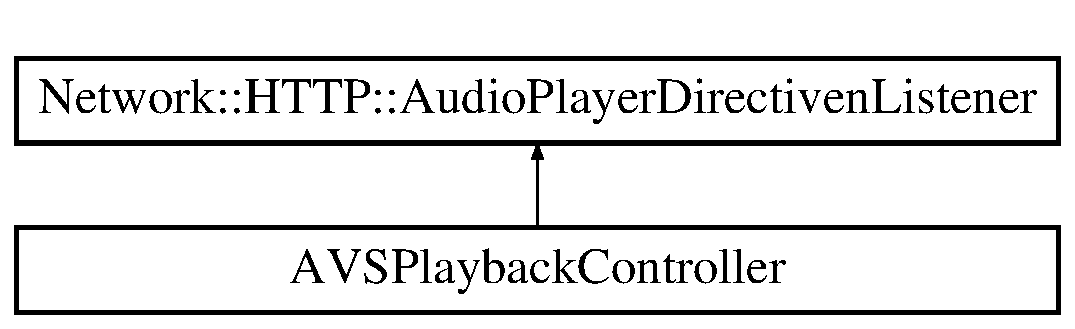
\includegraphics[height=2.000000cm]{d4/d02/classNetwork_1_1HTTP_1_1AudioPlayerDirectivenListener}
\end{center}
\end{figure}
\subsection*{Public Member Functions}
\begin{DoxyCompactItemize}
\item 
\mbox{\Hypertarget{classNetwork_1_1HTTP_1_1AudioPlayerDirectivenListener_a4ae61de51ef94365641ea7b330f81062}\label{classNetwork_1_1HTTP_1_1AudioPlayerDirectivenListener_a4ae61de51ef94365641ea7b330f81062}} 
virtual void {\bfseries on\+Play\+Directive} (const \hyperlink{classNetwork_1_1HTTP_1_1HTTPClientDirectiveEvent}{H\+T\+T\+P\+Client\+Directive\+Event} $\ast$event)=0
\item 
\mbox{\Hypertarget{classNetwork_1_1HTTP_1_1AudioPlayerDirectivenListener_a80b2a9267bbe821f109d0cc7feb7af92}\label{classNetwork_1_1HTTP_1_1AudioPlayerDirectivenListener_a80b2a9267bbe821f109d0cc7feb7af92}} 
virtual void {\bfseries on\+Stop\+Directive} (const \hyperlink{classNetwork_1_1HTTP_1_1HTTPClientDirectiveEvent}{H\+T\+T\+P\+Client\+Directive\+Event} $\ast$event)=0
\item 
\mbox{\Hypertarget{classNetwork_1_1HTTP_1_1AudioPlayerDirectivenListener_a67fed55016da69d39adc936d82099541}\label{classNetwork_1_1HTTP_1_1AudioPlayerDirectivenListener_a67fed55016da69d39adc936d82099541}} 
virtual void {\bfseries on\+Clear\+Queue\+Directive} (const \hyperlink{classNetwork_1_1HTTP_1_1HTTPClientDirectiveEvent}{H\+T\+T\+P\+Client\+Directive\+Event} $\ast$event)=0
\end{DoxyCompactItemize}


The documentation for this class was generated from the following file\+:\begin{DoxyCompactItemize}
\item 
/home/mutzi/progs/linux\+\_\+workspace/alexa-\/avs-\/prototype/src/include/directivenlistener.\+h\end{DoxyCompactItemize}

\hypertarget{classAVSApplication}{}\section{A\+V\+S\+Application Class Reference}
\label{classAVSApplication}\index{A\+V\+S\+Application@{A\+V\+S\+Application}}
Inheritance diagram for A\+V\+S\+Application\+:\begin{figure}[H]
\begin{center}
\leavevmode
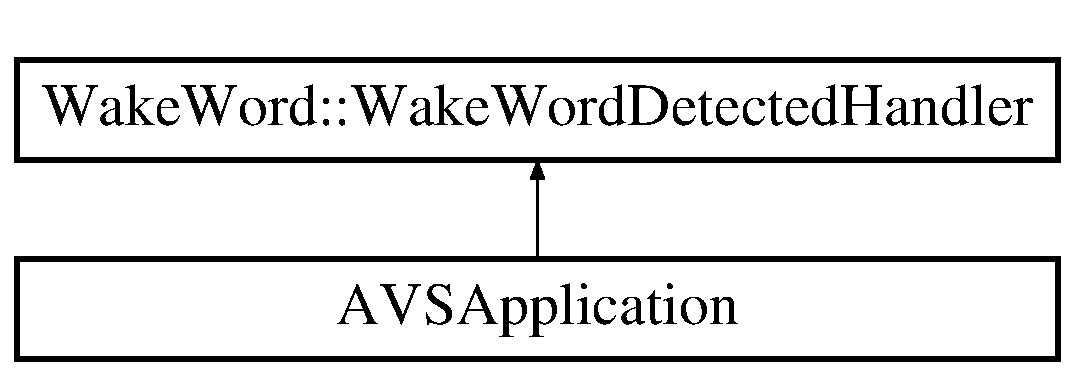
\includegraphics[height=2.000000cm]{d1/d36/classAVSApplication}
\end{center}
\end{figure}
\subsection*{Public Member Functions}
\begin{DoxyCompactItemize}
\item 
\mbox{\Hypertarget{classAVSApplication_a5f2565c654e3393cf1a1fe0787355b6d}\label{classAVSApplication_a5f2565c654e3393cf1a1fe0787355b6d}} 
void {\bfseries main} (int argc, char $\ast$$\ast$argv)
\item 
\mbox{\Hypertarget{classAVSApplication_a984f8e6e0d116c6adaef971a963ece5d}\label{classAVSApplication_a984f8e6e0d116c6adaef971a963ece5d}} 
void {\bfseries on\+Wake\+Word\+Detected} (void)
\end{DoxyCompactItemize}


The documentation for this class was generated from the following files\+:\begin{DoxyCompactItemize}
\item 
/home/mutzi/progs/linux\+\_\+workspace/alexa-\/avs-\/prototype/src/include/avsapplication.\+h\item 
/home/mutzi/progs/linux\+\_\+workspace/alexa-\/avs-\/prototype/src/avsapplication.\+cpp\end{DoxyCompactItemize}

\hypertarget{classAVSAuthenticator}{}\section{A\+V\+S\+Authenticator Class Reference}
\label{classAVSAuthenticator}\index{A\+V\+S\+Authenticator@{A\+V\+S\+Authenticator}}
Inheritance diagram for A\+V\+S\+Authenticator\+:\begin{figure}[H]
\begin{center}
\leavevmode
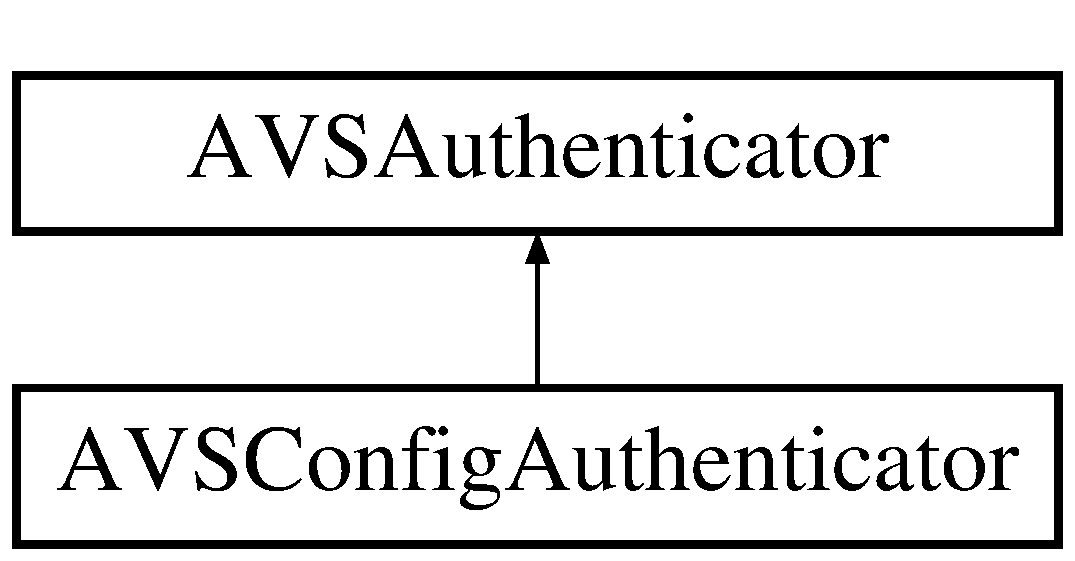
\includegraphics[height=2.000000cm]{d7/df0/classAVSAuthenticator}
\end{center}
\end{figure}
\subsection*{Public Member Functions}
\begin{DoxyCompactItemize}
\item 
\mbox{\Hypertarget{classAVSAuthenticator_a1f79451e5fa0c1390097e4ff73b5b40b}\label{classAVSAuthenticator_a1f79451e5fa0c1390097e4ff73b5b40b}} 
{\bfseries A\+V\+S\+Authenticator} (std\+::string client\+\_\+id, std\+::string client\+\_\+secret\+\_\+id, std\+::string client\+\_\+redirect\+\_\+uri, std\+::string product\+\_\+id)
\item 
\mbox{\Hypertarget{classAVSAuthenticator_ad7f0bc8ce2105bf1b6449e6ff86d5cbf}\label{classAVSAuthenticator_ad7f0bc8ce2105bf1b6449e6ff86d5cbf}} 
void {\bfseries set\+Client\+ID} (std\+::string client\+\_\+id)
\item 
\mbox{\Hypertarget{classAVSAuthenticator_a198c681ea8cc27f07556d4b756e4e38c}\label{classAVSAuthenticator_a198c681ea8cc27f07556d4b756e4e38c}} 
void {\bfseries set\+Client\+Secret\+ID} (std\+::string client\+\_\+secret\+\_\+id)
\item 
\mbox{\Hypertarget{classAVSAuthenticator_abcd468107452a7ad4b9c5dcfcf6b350e}\label{classAVSAuthenticator_abcd468107452a7ad4b9c5dcfcf6b350e}} 
void {\bfseries set\+Redirect\+U\+RI} (std\+::string redirect\+\_\+uri)
\item 
\mbox{\Hypertarget{classAVSAuthenticator_ab0f9175b2937a08ca40484618a808bda}\label{classAVSAuthenticator_ab0f9175b2937a08ca40484618a808bda}} 
void {\bfseries set\+Product\+ID} (std\+::string product\+\_\+id)
\item 
\mbox{\Hypertarget{classAVSAuthenticator_aa0e753cc2972da2dd5d6a7b010386549}\label{classAVSAuthenticator_aa0e753cc2972da2dd5d6a7b010386549}} 
void {\bfseries set\+Refresh\+Token} (std\+::string refresh\+\_\+token)
\item 
const std\+::string \hyperlink{classAVSAuthenticator_ad7c95c1a81852aff4c9bedb96da49ee8}{Generate\+Amazon\+Login\+Page} (void)
\begin{DoxyCompactList}\small\item\em Generate\+Amazon\+Login\+Page. \end{DoxyCompactList}\item 
const std\+::string \hyperlink{classAVSAuthenticator_ab08c84db0227d93f3a23713bd9970c95}{Generate\+Refresh\+Token} (const std\+::string code\+\_\+grant)  throw (\+Authenticator\+State)
\begin{DoxyCompactList}\small\item\em Generate\+Refresh\+Token. \end{DoxyCompactList}\item 
const std\+::string \hyperlink{classAVSAuthenticator_a501ad6b1063945e065ed00d5f25e7dd8}{Generate\+Access\+Token} (std\+::string refresh\+\_\+token)  throw (\+Authenticator\+State)
\begin{DoxyCompactList}\small\item\em Generate\+Access\+Token. \end{DoxyCompactList}\item 
\mbox{\Hypertarget{classAVSAuthenticator_a36556663a3cddcea619c4990a6f1b3ef}\label{classAVSAuthenticator_a36556663a3cddcea619c4990a6f1b3ef}} 
const std\+::string {\bfseries get\+Last\+Code\+Grant} (void) const
\item 
\mbox{\Hypertarget{classAVSAuthenticator_a5e81f4f68736463f984b86636d7aad46}\label{classAVSAuthenticator_a5e81f4f68736463f984b86636d7aad46}} 
const std\+::string {\bfseries get\+Last\+Access\+Token} (void) const
\item 
\mbox{\Hypertarget{classAVSAuthenticator_a3b15ba2b326d91dd4e416f040eb31e6e}\label{classAVSAuthenticator_a3b15ba2b326d91dd4e416f040eb31e6e}} 
const std\+::string {\bfseries get\+Refresh\+Token} (void) const
\end{DoxyCompactItemize}
\subsection*{Protected Member Functions}
\begin{DoxyCompactItemize}
\item 
\mbox{\Hypertarget{classAVSAuthenticator_a16f585dde9b8f3a57f63a2a2efdb6bb3}\label{classAVSAuthenticator_a16f585dde9b8f3a57f63a2a2efdb6bb3}} 
std\+::string {\bfseries response\+\_\+analyse\+\_\+refresh\+\_\+token} (\hyperlink{classNetwork_1_1HTTP_1_1HTTPResponse}{H\+T\+T\+P\+Response} $\ast$response)
\item 
\mbox{\Hypertarget{classAVSAuthenticator_a10b289223c265cf3d5e42eef181839ea}\label{classAVSAuthenticator_a10b289223c265cf3d5e42eef181839ea}} 
std\+::string {\bfseries response\+\_\+analyse\+\_\+access\+\_\+token} (\hyperlink{classNetwork_1_1HTTP_1_1HTTPResponse}{H\+T\+T\+P\+Response} $\ast$response)
\item 
\mbox{\Hypertarget{classAVSAuthenticator_ab886240a85b2c530286e976af9a62a9c}\label{classAVSAuthenticator_ab886240a85b2c530286e976af9a62a9c}} 
void {\bfseries url\+\_\+encode} (std\+::string content)
\item 
\mbox{\Hypertarget{classAVSAuthenticator_ae88efd94941043ac454a2587031ab74e}\label{classAVSAuthenticator_ae88efd94941043ac454a2587031ab74e}} 
void {\bfseries replace} (string \&str, string search, string replace)
\end{DoxyCompactItemize}


\subsection{Member Function Documentation}
\mbox{\Hypertarget{classAVSAuthenticator_a501ad6b1063945e065ed00d5f25e7dd8}\label{classAVSAuthenticator_a501ad6b1063945e065ed00d5f25e7dd8}} 
\index{A\+V\+S\+Authenticator@{A\+V\+S\+Authenticator}!Generate\+Access\+Token@{Generate\+Access\+Token}}
\index{Generate\+Access\+Token@{Generate\+Access\+Token}!A\+V\+S\+Authenticator@{A\+V\+S\+Authenticator}}
\subsubsection{\texorpdfstring{Generate\+Access\+Token()}{GenerateAccessToken()}}
{\footnotesize\ttfamily const std\+::string A\+V\+S\+Authenticator\+::\+Generate\+Access\+Token (\begin{DoxyParamCaption}\item[{std\+::string}]{refresh\+\_\+token }\end{DoxyParamCaption}) throw  Authenticator\+State) }



Generate\+Access\+Token. 

Generate new Access\+Tokens from Refresh\+Token 
\begin{DoxyParams}{Parameters}
{\em refresh\+\_\+token} & \\
\hline
\end{DoxyParams}
\begin{DoxyReturn}{Returns}

\end{DoxyReturn}
\mbox{\Hypertarget{classAVSAuthenticator_ad7c95c1a81852aff4c9bedb96da49ee8}\label{classAVSAuthenticator_ad7c95c1a81852aff4c9bedb96da49ee8}} 
\index{A\+V\+S\+Authenticator@{A\+V\+S\+Authenticator}!Generate\+Amazon\+Login\+Page@{Generate\+Amazon\+Login\+Page}}
\index{Generate\+Amazon\+Login\+Page@{Generate\+Amazon\+Login\+Page}!A\+V\+S\+Authenticator@{A\+V\+S\+Authenticator}}
\subsubsection{\texorpdfstring{Generate\+Amazon\+Login\+Page()}{GenerateAmazonLoginPage()}}
{\footnotesize\ttfamily const std\+::string A\+V\+S\+Authenticator\+::\+Generate\+Amazon\+Login\+Page (\begin{DoxyParamCaption}\item[{void}]{ }\end{DoxyParamCaption})}



Generate\+Amazon\+Login\+Page. 

G\+ET Amazon Login Page $\vert$=$>$ Login \& get C\+O\+DE G\+R\+A\+NT \begin{DoxyReturn}{Returns}

\end{DoxyReturn}
\mbox{\Hypertarget{classAVSAuthenticator_ab08c84db0227d93f3a23713bd9970c95}\label{classAVSAuthenticator_ab08c84db0227d93f3a23713bd9970c95}} 
\index{A\+V\+S\+Authenticator@{A\+V\+S\+Authenticator}!Generate\+Refresh\+Token@{Generate\+Refresh\+Token}}
\index{Generate\+Refresh\+Token@{Generate\+Refresh\+Token}!A\+V\+S\+Authenticator@{A\+V\+S\+Authenticator}}
\subsubsection{\texorpdfstring{Generate\+Refresh\+Token()}{GenerateRefreshToken()}}
{\footnotesize\ttfamily const std\+::string A\+V\+S\+Authenticator\+::\+Generate\+Refresh\+Token (\begin{DoxyParamCaption}\item[{const std\+::string}]{code\+\_\+grant }\end{DoxyParamCaption}) throw  Authenticator\+State) }



Generate\+Refresh\+Token. 

Generate Refresh\+Token from C\+O\+DE G\+R\+A\+NT 
\begin{DoxyParams}{Parameters}
{\em code\+\_\+grant} & \\
\hline
\end{DoxyParams}
\begin{DoxyReturn}{Returns}

\end{DoxyReturn}


The documentation for this class was generated from the following files\+:\begin{DoxyCompactItemize}
\item 
/home/mutzi/progs/linux\+\_\+workspace/alexa-\/avs-\/prototype/src/include/avsauthenticator.\+h\item 
/home/mutzi/progs/linux\+\_\+workspace/alexa-\/avs-\/prototype/src/avsauthenticator.\+cpp\end{DoxyCompactItemize}

\hypertarget{classAVSClient}{}\section{A\+V\+S\+Client Class Reference}
\label{classAVSClient}\index{A\+V\+S\+Client@{A\+V\+S\+Client}}
Inheritance diagram for A\+V\+S\+Client\+:\begin{figure}[H]
\begin{center}
\leavevmode
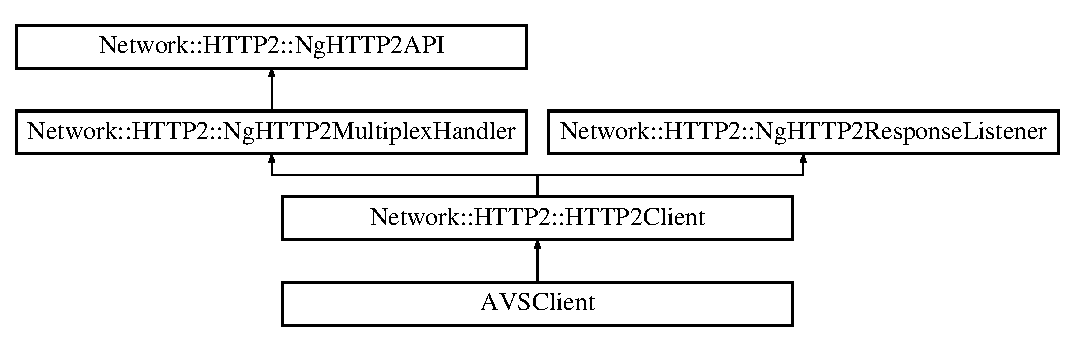
\includegraphics[height=4.000000cm]{d0/db9/classAVSClient}
\end{center}
\end{figure}
\subsection*{Public Member Functions}
\begin{DoxyCompactItemize}
\item 
\mbox{\Hypertarget{classAVSClient_ae0d7c3e648fc864ae436831e17f794e2}\label{classAVSClient_ae0d7c3e648fc864ae436831e17f794e2}} 
{\bfseries A\+V\+S\+Client} (const std\+::string url, const std\+::string access\+\_\+token)
\item 
\mbox{\Hypertarget{classAVSClient_a23465de5d4163ee26d9576e721f6f0c6}\label{classAVSClient_a23465de5d4163ee26d9576e721f6f0c6}} 
void {\bfseries add\+Listener} (\hyperlink{classAVSClientListener}{A\+V\+S\+Client\+Listener} $\ast$listener)
\item 
\mbox{\Hypertarget{classAVSClient_a634dd701d7f6f6e6bdb31d7f5abaa51c}\label{classAVSClient_a634dd701d7f6f6e6bdb31d7f5abaa51c}} 
void {\bfseries remove\+Listener} (\hyperlink{classAVSClientListener}{A\+V\+S\+Client\+Listener} $\ast$listener)
\item 
\mbox{\Hypertarget{classAVSClient_a1f9560eb150c6ef158af1541c7cde899}\label{classAVSClient_a1f9560eb150c6ef158af1541c7cde899}} 
void {\bfseries start} (void)
\item 
\mbox{\Hypertarget{classAVSClient_a013525f5bcb5608feda51c45504a1c38}\label{classAVSClient_a013525f5bcb5608feda51c45504a1c38}} 
void {\bfseries restart} (void)
\item 
\mbox{\Hypertarget{classAVSClient_a3f4655c808ea71fc7d9192a277daca00}\label{classAVSClient_a3f4655c808ea71fc7d9192a277daca00}} 
void {\bfseries change\+Access\+Token} (const std\+::string access\+\_\+token)
\item 
\mbox{\Hypertarget{classAVSClient_a9af7374fe03aa49a3557c3fd574a6c58}\label{classAVSClient_a9af7374fe03aa49a3557c3fd574a6c58}} 
\hyperlink{classAVSRequestBuilder}{A\+V\+S\+Request\+Builder} $\ast$ {\bfseries get\+Request\+Builder} (void)
\item 
\mbox{\Hypertarget{classAVSClient_ac1d14f5bbf23b2b7c108887b45a7247f}\label{classAVSClient_ac1d14f5bbf23b2b7c108887b45a7247f}} 
\hyperlink{structAVSJson_1_1SynchronizeStateEvent}{A\+V\+S\+Json\+::\+Synchronize\+State\+Event} $\ast$ {\bfseries get\+Sync\+State} (void)
\item 
\mbox{\Hypertarget{classAVSClient_a7ec5d02b02e8ea15e4d79c155bed41e7}\label{classAVSClient_a7ec5d02b02e8ea15e4d79c155bed41e7}} 
bool {\bfseries is\+Active} (void)
\item 
\mbox{\Hypertarget{classAVSClient_ae11fec4bb36751971307088aa68e9c5d}\label{classAVSClient_ae11fec4bb36751971307088aa68e9c5d}} 
\hyperlink{structNetwork_1_1HTTP2_1_1StreamQueueData}{Stream\+Queue\+Data} $\ast$ {\bfseries on\+Process\+Stream\+Event} (Stream\+Queue\+Event event)
\item 
\mbox{\Hypertarget{classAVSClient_a8d9ca62de50e2f1c8f9131277728b170}\label{classAVSClient_a8d9ca62de50e2f1c8f9131277728b170}} 
void {\bfseries on\+Stream\+Loop\+Start\+Event} (void)
\item 
\mbox{\Hypertarget{classAVSClient_a8371fdf83e36adee3292958e13db684e}\label{classAVSClient_a8371fdf83e36adee3292958e13db684e}} 
void {\bfseries on\+Stream\+Loop\+Wait\+Event} (void)
\end{DoxyCompactItemize}
\subsection*{Additional Inherited Members}


The documentation for this class was generated from the following files\+:\begin{DoxyCompactItemize}
\item 
/home/mutzi/progs/linux\+\_\+workspace/alexa-\/avs-\/prototype/src/include/avsclient.\+h\item 
/home/mutzi/progs/linux\+\_\+workspace/alexa-\/avs-\/prototype/src/avsclient.\+cpp\end{DoxyCompactItemize}

\hypertarget{classAVSClientListener}{}\section{A\+V\+S\+Client\+Listener Class Reference}
\label{classAVSClientListener}\index{A\+V\+S\+Client\+Listener@{A\+V\+S\+Client\+Listener}}
Inheritance diagram for A\+V\+S\+Client\+Listener\+:\begin{figure}[H]
\begin{center}
\leavevmode
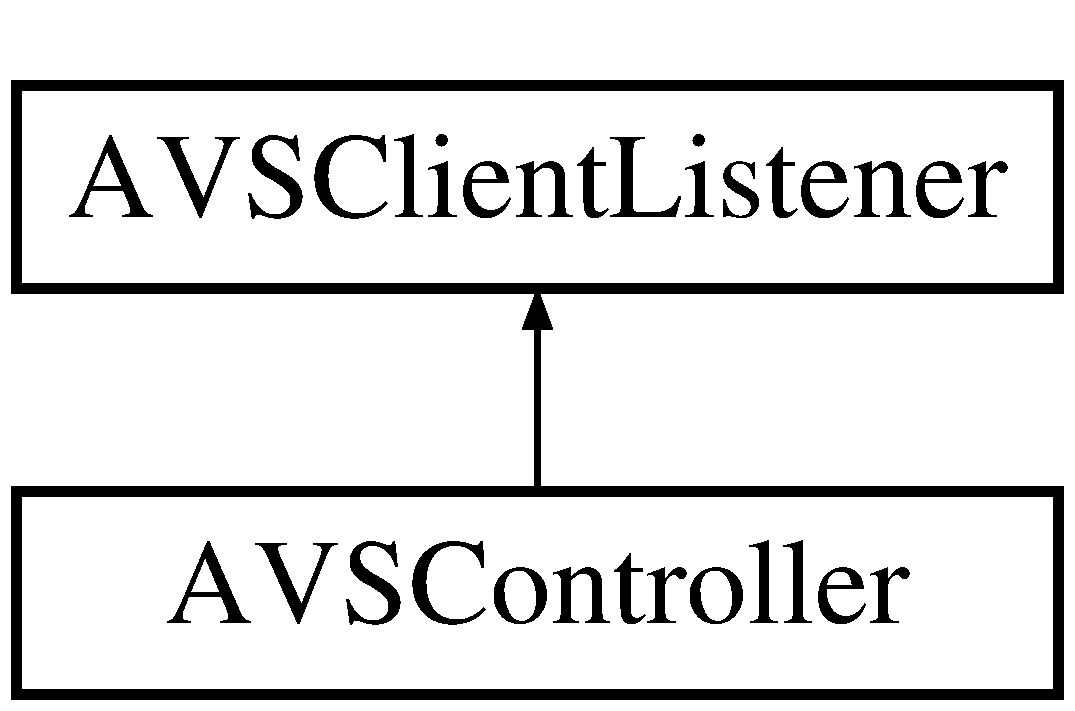
\includegraphics[height=2.000000cm]{d5/d2c/classAVSClientListener}
\end{center}
\end{figure}
\subsection*{Public Member Functions}
\begin{DoxyCompactItemize}
\item 
\mbox{\Hypertarget{classAVSClientListener_a832446639c6b2f171a75a925badac576}\label{classAVSClientListener_a832446639c6b2f171a75a925badac576}} 
virtual void {\bfseries on\+Stream\+Loop\+Start\+Event} (void)=0
\item 
\mbox{\Hypertarget{classAVSClientListener_aba46eb1768eb5abdfb01c7d3ef3768c9}\label{classAVSClientListener_aba46eb1768eb5abdfb01c7d3ef3768c9}} 
virtual void {\bfseries on\+Stream\+Loop\+Wait\+Event} (void)=0
\item 
\mbox{\Hypertarget{classAVSClientListener_a2dda4af7731de612043954d1a9abcb18}\label{classAVSClientListener_a2dda4af7731de612043954d1a9abcb18}} 
virtual void {\bfseries on\+Device\+Capture\+Open\+Event} (void)=0
\item 
\mbox{\Hypertarget{classAVSClientListener_a12db20d06801d1af8fb77211a4a2eeb5}\label{classAVSClientListener_a12db20d06801d1af8fb77211a4a2eeb5}} 
virtual void {\bfseries on\+Device\+Capture\+Close\+Event} (void)=0
\end{DoxyCompactItemize}


The documentation for this class was generated from the following file\+:\begin{DoxyCompactItemize}
\item 
/home/mutzi/progs/linux\+\_\+workspace/alexa-\/avs-\/prototype/src/include/avsclientlistener.\+h\end{DoxyCompactItemize}

\hypertarget{classAVSConfigAuthenticator}{}\section{A\+V\+S\+Config\+Authenticator Class Reference}
\label{classAVSConfigAuthenticator}\index{A\+V\+S\+Config\+Authenticator@{A\+V\+S\+Config\+Authenticator}}
Inheritance diagram for A\+V\+S\+Config\+Authenticator\+:\begin{figure}[H]
\begin{center}
\leavevmode
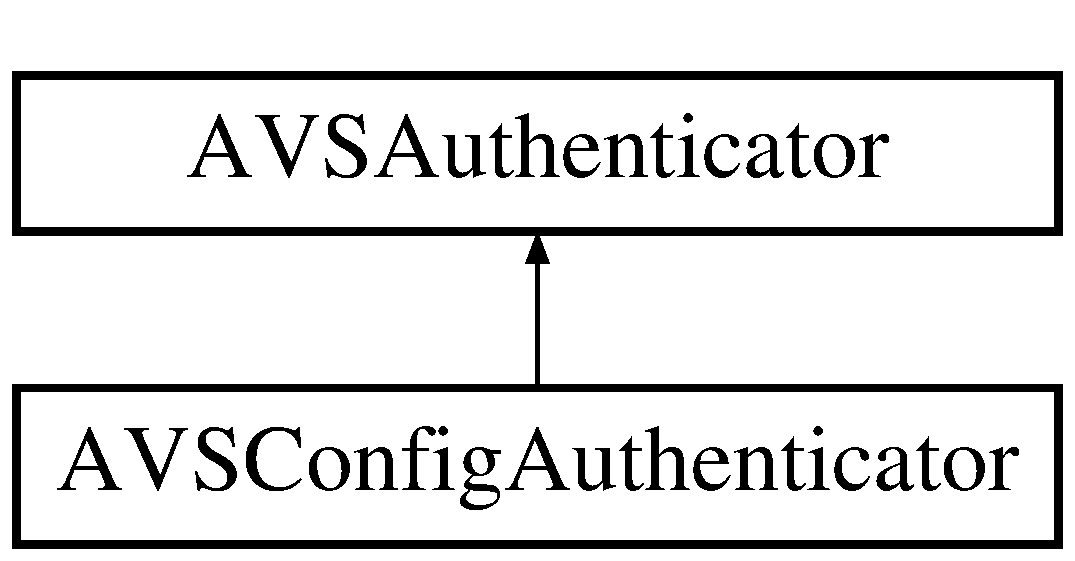
\includegraphics[height=2.000000cm]{d0/da2/classAVSConfigAuthenticator}
\end{center}
\end{figure}
\subsection*{Public Member Functions}
\begin{DoxyCompactItemize}
\item 
\mbox{\Hypertarget{classAVSConfigAuthenticator_a4034cc73e6d7540b47635b0e0bd23dcc}\label{classAVSConfigAuthenticator_a4034cc73e6d7540b47635b0e0bd23dcc}} 
{\bfseries A\+V\+S\+Config\+Authenticator} (const std\+::string \&config\+\_\+file)
\item 
\mbox{\Hypertarget{classAVSConfigAuthenticator_ad3e1966ff0a56c3ccb38c0ae82db4767}\label{classAVSConfigAuthenticator_ad3e1966ff0a56c3ccb38c0ae82db4767}} 
void {\bfseries read\+Config} ()
\end{DoxyCompactItemize}
\subsection*{Protected Member Functions}
\begin{DoxyCompactItemize}
\item 
\mbox{\Hypertarget{classAVSConfigAuthenticator_a4c2cd0d9123ece1cb738f2d69d12728e}\label{classAVSConfigAuthenticator_a4c2cd0d9123ece1cb738f2d69d12728e}} 
void {\bfseries on\+Event\+Error\+Set} (const std\+::string name)
\end{DoxyCompactItemize}


The documentation for this class was generated from the following files\+:\begin{DoxyCompactItemize}
\item 
/home/mutzi/progs/linux\+\_\+workspace/alexa-\/avs-\/prototype/src/include/avsconfigauthenticator.\+h\item 
/home/mutzi/progs/linux\+\_\+workspace/alexa-\/avs-\/prototype/src/avsconfigauthenticator.\+cpp\end{DoxyCompactItemize}

\hypertarget{classAVSController}{}\section{A\+V\+S\+Controller Class Reference}
\label{classAVSController}\index{A\+V\+S\+Controller@{A\+V\+S\+Controller}}
Inheritance diagram for A\+V\+S\+Controller\+:\begin{figure}[H]
\begin{center}
\leavevmode
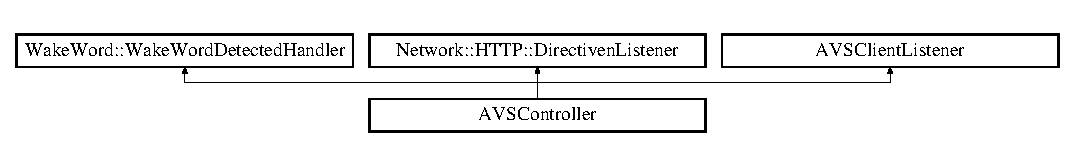
\includegraphics[height=1.536351cm]{d3/d4e/classAVSController}
\end{center}
\end{figure}
\subsection*{Public Member Functions}
\begin{DoxyCompactItemize}
\item 
\mbox{\Hypertarget{classAVSController_a63d0d4f3504598a6cf631d743221148c}\label{classAVSController_a63d0d4f3504598a6cf631d743221148c}} 
{\bfseries A\+V\+S\+Controller} (\hyperlink{classWakeWord_1_1WakeWordIPCFactory}{Wake\+Word\+I\+P\+C\+Factory} $\ast$wake\+Word\+I\+P\+C\+Factory, \hyperlink{classWakeWord_1_1WakeWordDetectedHandler}{Wake\+Word\+Detected\+Handler} $\ast$wake\+Word\+Detected\+Handler)  throw ( std\+::exception )
\item 
\mbox{\Hypertarget{classAVSController_a7e82175b8fa5864d1ec17509dc0298c9}\label{classAVSController_a7e82175b8fa5864d1ec17509dc0298c9}} 
void {\bfseries start\+A\+V\+S\+Client} (void)
\item 
\mbox{\Hypertarget{classAVSController_aaf6ac00abc79561f81fe932df6226ec0}\label{classAVSController_aaf6ac00abc79561f81fe932df6226ec0}} 
void {\bfseries start\+Wake\+Word\+Server} (void)
\item 
\mbox{\Hypertarget{classAVSController_a68695f1c999d840021878ca1eaa4ac78}\label{classAVSController_a68695f1c999d840021878ca1eaa4ac78}} 
void {\bfseries send\+Wake\+Word\+Signal} (I\+P\+C\+Command command)
\item 
\mbox{\Hypertarget{classAVSController_af4e3b90cc19b84dc38a6035dfa7fc700}\label{classAVSController_af4e3b90cc19b84dc38a6035dfa7fc700}} 
void {\bfseries start\+Audio\+Streaming} (void)
\item 
\mbox{\Hypertarget{classAVSController_ab692b03c8cdb638ef397c2a983bb43b1}\label{classAVSController_ab692b03c8cdb638ef397c2a983bb43b1}} 
void {\bfseries stop\+Audio\+Streaming} (void)
\item 
\mbox{\Hypertarget{classAVSController_ae0c0e24cfb2a347ceaf16698f1971c52}\label{classAVSController_ae0c0e24cfb2a347ceaf16698f1971c52}} 
\hyperlink{classAVSClient}{A\+V\+S\+Client} $\ast$ {\bfseries get\+A\+V\+S\+Client} (void)
\item 
\mbox{\Hypertarget{classAVSController_a5e28e26ddb32663fe918809cd2da50b5}\label{classAVSController_a5e28e26ddb32663fe918809cd2da50b5}} 
\hyperlink{classAVSConfigAuthenticator}{A\+V\+S\+Config\+Authenticator} $\ast$ {\bfseries get\+Authenticator} (void)
\item 
\mbox{\Hypertarget{classAVSController_ae1a6b6f95f9e2ac206e2724e33f57741}\label{classAVSController_ae1a6b6f95f9e2ac206e2724e33f57741}} 
\hyperlink{classAVSPlayback}{A\+V\+S\+Playback} $\ast$ {\bfseries get\+A\+V\+S\+Playback\+Handle} (void)
\end{DoxyCompactItemize}
\subsection*{Static Public Member Functions}
\begin{DoxyCompactItemize}
\item 
\mbox{\Hypertarget{classAVSController_a00967eb8be7b2d3764acd1cb669ef775}\label{classAVSController_a00967eb8be7b2d3764acd1cb669ef775}} 
static void {\bfseries playback\+\_\+thread} (\hyperlink{classAVSController}{A\+V\+S\+Controller} $\ast$controller, char $\ast$mp3data, size\+\_\+t mp3size)
\item 
\mbox{\Hypertarget{classAVSController_a6e5a0581df44aa4500d3ac7601e98494}\label{classAVSController_a6e5a0581df44aa4500d3ac7601e98494}} 
static void {\bfseries playback\+\_\+mute\+\_\+thread} (\hyperlink{classAVSPlayback}{A\+V\+S\+Playback} $\ast$playback\+\_\+handle)
\item 
\mbox{\Hypertarget{classAVSController_ad6d9344629573dba5b0de01c1c9c56c8}\label{classAVSController_ad6d9344629573dba5b0de01c1c9c56c8}} 
static void {\bfseries playback\+\_\+unmute\+\_\+thread} (\hyperlink{classAVSPlayback}{A\+V\+S\+Playback} $\ast$playback\+\_\+handle)
\end{DoxyCompactItemize}
\subsection*{Protected Member Functions}
\begin{DoxyCompactItemize}
\item 
\mbox{\Hypertarget{classAVSController_a0f68ded5ebd1d728ca56e61a46ede630}\label{classAVSController_a0f68ded5ebd1d728ca56e61a46ede630}} 
void {\bfseries on\+Stream\+Loop\+Start\+Event} (void)
\item 
\mbox{\Hypertarget{classAVSController_a67d0ffd826dc595aa23e8fdfe3e45422}\label{classAVSController_a67d0ffd826dc595aa23e8fdfe3e45422}} 
void {\bfseries on\+Stream\+Loop\+Wait\+Event} (void)
\item 
\mbox{\Hypertarget{classAVSController_a93119243f11d797554d6a175f30ff391}\label{classAVSController_a93119243f11d797554d6a175f30ff391}} 
void {\bfseries on\+Device\+Capture\+Open\+Event} (void)
\item 
\mbox{\Hypertarget{classAVSController_aca4f642e82b469cda941822ab74770c5}\label{classAVSController_aca4f642e82b469cda941822ab74770c5}} 
void {\bfseries on\+Device\+Capture\+Close\+Event} (void)
\item 
\mbox{\Hypertarget{classAVSController_a149bd119bb25bf57850ac9978158d408}\label{classAVSController_a149bd119bb25bf57850ac9978158d408}} 
void {\bfseries on\+Wake\+Word\+Detected} ()
\item 
\mbox{\Hypertarget{classAVSController_a81ab91d6a582db9636a82b3c9f620e63}\label{classAVSController_a81ab91d6a582db9636a82b3c9f620e63}} 
void {\bfseries on\+Speech\+Recognize\+Stop\+Capture\+Directive} (const \hyperlink{classNetwork_1_1HTTP_1_1HTTPClientDirectiveEvent}{H\+T\+T\+P\+Client\+Directive\+Event} $\ast$event)
\item 
\mbox{\Hypertarget{classAVSController_a9fa9fb34684b7ea46f97926fbabbd31d}\label{classAVSController_a9fa9fb34684b7ea46f97926fbabbd31d}} 
void {\bfseries on\+Speech\+Recognize\+Expect\+Speech\+Directive} (const \hyperlink{classNetwork_1_1HTTP_1_1HTTPClientDirectiveEvent}{H\+T\+T\+P\+Client\+Directive\+Event} $\ast$event)
\item 
\mbox{\Hypertarget{classAVSController_ae6275a874383c8be50efbc4b420eaab2}\label{classAVSController_ae6275a874383c8be50efbc4b420eaab2}} 
void {\bfseries on\+Speech\+Synthesizer\+Speak\+Directive} (const \hyperlink{classNetwork_1_1HTTP_1_1HTTPClientDirectiveEvent}{H\+T\+T\+P\+Client\+Directive\+Event} $\ast$event)
\item 
\mbox{\Hypertarget{classAVSController_a9226e5badeb17e54fa2cb32f9973cc89}\label{classAVSController_a9226e5badeb17e54fa2cb32f9973cc89}} 
void {\bfseries on\+Speeker\+Set\+Mute\+Directive} (const \hyperlink{classNetwork_1_1HTTP_1_1HTTPClientDirectiveEvent}{H\+T\+T\+P\+Client\+Directive\+Event} $\ast$event)
\end{DoxyCompactItemize}


The documentation for this class was generated from the following files\+:\begin{DoxyCompactItemize}
\item 
/home/mutzi/progs/linux\+\_\+workspace/alexa-\/avs-\/prototype/src/include/avscontroller.\+h\item 
/home/mutzi/progs/linux\+\_\+workspace/alexa-\/avs-\/prototype/src/avscontroller.\+cpp\end{DoxyCompactItemize}

\hypertarget{structAVSHeaderData}{}\section{A\+V\+S\+Header\+Data Struct Reference}
\label{structAVSHeaderData}\index{A\+V\+S\+Header\+Data@{A\+V\+S\+Header\+Data}}
\subsection*{Public Attributes}
\begin{DoxyCompactItemize}
\item 
\mbox{\Hypertarget{structAVSHeaderData_a6834b76cb79fd89038782a0b32d5a6a3}\label{structAVSHeaderData_a6834b76cb79fd89038782a0b32d5a6a3}} 
nghttp2\+\_\+nv $\ast$ {\bfseries header}
\item 
\mbox{\Hypertarget{structAVSHeaderData_abd96071f0a22c3e81f4c95c46af3f8cb}\label{structAVSHeaderData_abd96071f0a22c3e81f4c95c46af3f8cb}} 
size\+\_\+t {\bfseries header\+\_\+len}
\end{DoxyCompactItemize}


The documentation for this struct was generated from the following file\+:\begin{DoxyCompactItemize}
\item 
/home/mutzi/progs/linux\+\_\+workspace/alexa-\/avs-\/prototype/src/include/avsrequestbuilder.\+h\end{DoxyCompactItemize}

\hypertarget{classAVSLame}{}\section{A\+V\+S\+Lame Class Reference}
\label{classAVSLame}\index{A\+V\+S\+Lame@{A\+V\+S\+Lame}}
\subsection*{Public Member Functions}
\begin{DoxyCompactItemize}
\item 
\mbox{\Hypertarget{classAVSLame_a2977e3fbc07edbd5e4ff26ce75ec2c3a}\label{classAVSLame_a2977e3fbc07edbd5e4ff26ce75ec2c3a}} 
int {\bfseries set\+\_\+in\+\_\+samplerate} (int rate)
\item 
\mbox{\Hypertarget{classAVSLame_afe00737f2c83816810bc9291ed77d3a5}\label{classAVSLame_afe00737f2c83816810bc9291ed77d3a5}} 
int {\bfseries set\+\_\+\+V\+BR} (vbr\+\_\+mode mode)
\item 
\mbox{\Hypertarget{classAVSLame_acd6bb2f86cc6ee36af118731f7719899}\label{classAVSLame_acd6bb2f86cc6ee36af118731f7719899}} 
int {\bfseries set\+\_\+decode\+\_\+only} (int)
\item 
\mbox{\Hypertarget{classAVSLame_a2accad11b80380e7ca6186ea37ebac07}\label{classAVSLame_a2accad11b80380e7ca6186ea37ebac07}} 
int {\bfseries init\+\_\+params} ()
\item 
\mbox{\Hypertarget{classAVSLame_a8bb4dbb0eb60474877d94cd52c6d5a53}\label{classAVSLame_a8bb4dbb0eb60474877d94cd52c6d5a53}} 
int {\bfseries decode1\+\_\+headers\+\_\+mp3data} (unsigned char $\ast$mp3\+\_\+buf, size\+\_\+t mp3\+\_\+len, short pcm\+\_\+l\mbox{[}$\,$\mbox{]}, short pcm\+\_\+r\mbox{[}$\,$\mbox{]}, mp3data\+\_\+struct $\ast$mp3\+\_\+data)
\item 
\mbox{\Hypertarget{classAVSLame_ab4db8b6f69070c03b0367f60ba2cef77}\label{classAVSLame_ab4db8b6f69070c03b0367f60ba2cef77}} 
int {\bfseries decode1\+\_\+headers} (unsigned char $\ast$mp3\+\_\+buf, size\+\_\+t mp3\+\_\+len, short pcm\+\_\+l\mbox{[}$\,$\mbox{]}, short pcm\+\_\+r\mbox{[}$\,$\mbox{]})
\item 
\mbox{\Hypertarget{classAVSLame_afefc95436db90a56de77f55843e5db22}\label{classAVSLame_afefc95436db90a56de77f55843e5db22}} 
int {\bfseries decode1} (unsigned char $\ast$mp3\+\_\+buf, size\+\_\+t mp3\+\_\+len, short pcm\+\_\+l\mbox{[}$\,$\mbox{]}, short pcm\+\_\+r\mbox{[}$\,$\mbox{]})
\end{DoxyCompactItemize}


The documentation for this class was generated from the following files\+:\begin{DoxyCompactItemize}
\item 
/home/mutzi/progs/linux\+\_\+workspace/alexa-\/avs-\/prototype/src/include/avslame.\+h\item 
/home/mutzi/progs/linux\+\_\+workspace/alexa-\/avs-\/prototype/src/avslame.\+cpp\end{DoxyCompactItemize}

\hypertarget{classAVSPlayback}{}\section{A\+V\+S\+Playback Class Reference}
\label{classAVSPlayback}\index{A\+V\+S\+Playback@{A\+V\+S\+Playback}}
\subsection*{Public Member Functions}
\begin{DoxyCompactItemize}
\item 
void \hyperlink{classAVSPlayback_a2460eb0d8552541d3cc44fde4156147e}{mute} (void)
\begin{DoxyCompactList}\small\item\em cancel \end{DoxyCompactList}\item 
\mbox{\Hypertarget{classAVSPlayback_ab5db8e18e9864da57915ce8d0c50199d}\label{classAVSPlayback_ab5db8e18e9864da57915ce8d0c50199d}} 
void {\bfseries unmute} (void)
\item 
void \hyperlink{classAVSPlayback_a4696222c7fd236d08811c79f1d90def3}{mp3\+Playback} (char $\ast$mp3\+\_\+data, size\+\_\+t mp3data\+\_\+size)
\begin{DoxyCompactList}\small\item\em mp3\+Playback \end{DoxyCompactList}\end{DoxyCompactItemize}


\subsection{Member Function Documentation}
\mbox{\Hypertarget{classAVSPlayback_a4696222c7fd236d08811c79f1d90def3}\label{classAVSPlayback_a4696222c7fd236d08811c79f1d90def3}} 
\index{A\+V\+S\+Playback@{A\+V\+S\+Playback}!mp3\+Playback@{mp3\+Playback}}
\index{mp3\+Playback@{mp3\+Playback}!A\+V\+S\+Playback@{A\+V\+S\+Playback}}
\subsubsection{\texorpdfstring{mp3\+Playback()}{mp3Playback()}}
{\footnotesize\ttfamily void A\+V\+S\+Playback\+::mp3\+Playback (\begin{DoxyParamCaption}\item[{char $\ast$}]{mp3\+\_\+data,  }\item[{size\+\_\+t}]{mp3data\+\_\+size }\end{DoxyParamCaption})}



mp3\+Playback 

Use libmp3lame play mp3 audio


\begin{DoxyParams}{Parameters}
{\em mp3\+\_\+data} & \\
\hline
{\em mp3data\+\_\+size} & \\
\hline
\end{DoxyParams}
\mbox{\Hypertarget{classAVSPlayback_a2460eb0d8552541d3cc44fde4156147e}\label{classAVSPlayback_a2460eb0d8552541d3cc44fde4156147e}} 
\index{A\+V\+S\+Playback@{A\+V\+S\+Playback}!mute@{mute}}
\index{mute@{mute}!A\+V\+S\+Playback@{A\+V\+S\+Playback}}
\subsubsection{\texorpdfstring{mute()}{mute()}}
{\footnotesize\ttfamily void A\+V\+S\+Playback\+::mute (\begin{DoxyParamCaption}\item[{void}]{ }\end{DoxyParamCaption})}



cancel 

cancel Audio playback Thread Safe 

The documentation for this class was generated from the following files\+:\begin{DoxyCompactItemize}
\item 
/home/mutzi/progs/linux\+\_\+workspace/alexa-\/avs-\/prototype/src/include/avsplayback.\+h\item 
/home/mutzi/progs/linux\+\_\+workspace/alexa-\/avs-\/prototype/src/avsplayback.\+cpp\end{DoxyCompactItemize}

\hypertarget{classAVSPlaybackController}{}\section{A\+V\+S\+Playback\+Controller Class Reference}
\label{classAVSPlaybackController}\index{A\+V\+S\+Playback\+Controller@{A\+V\+S\+Playback\+Controller}}
Inheritance diagram for A\+V\+S\+Playback\+Controller\+:\begin{figure}[H]
\begin{center}
\leavevmode
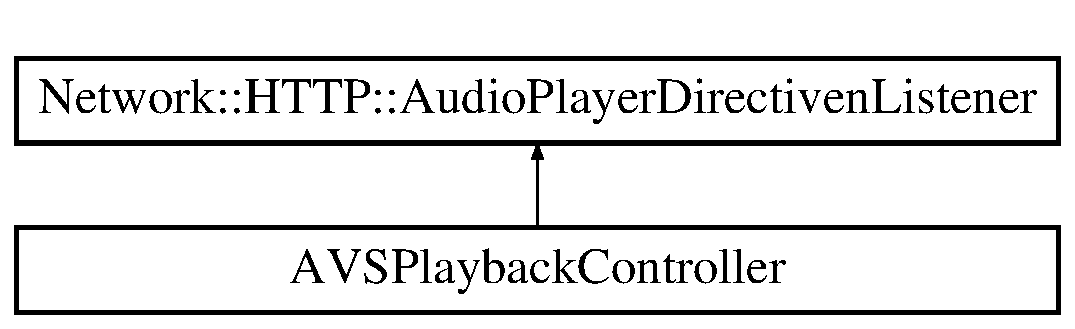
\includegraphics[height=2.000000cm]{dd/dca/classAVSPlaybackController}
\end{center}
\end{figure}
\subsection*{Public Member Functions}
\begin{DoxyCompactItemize}
\item 
\mbox{\Hypertarget{classAVSPlaybackController_adb98c7112a30f235cd147fe9ae06ef5d}\label{classAVSPlaybackController_adb98c7112a30f235cd147fe9ae06ef5d}} 
{\bfseries A\+V\+S\+Playback\+Controller} (\hyperlink{classAVSClient}{A\+V\+S\+Client} $\ast$avs\+\_\+client)
\item 
\mbox{\Hypertarget{classAVSPlaybackController_aa8558bffc088fe6e432873e2e5b168f1}\label{classAVSPlaybackController_aa8558bffc088fe6e432873e2e5b168f1}} 
void {\bfseries init\+Playback\+Thread} (void)
\item 
\mbox{\Hypertarget{classAVSPlaybackController_a0a26c091f4820d069c4ab1fc2c2d6b09}\label{classAVSPlaybackController_a0a26c091f4820d069c4ab1fc2c2d6b09}} 
void {\bfseries push\+Playback\+Queue} (\hyperlink{structPlaybackQueue}{Playback\+Queue} queue)
\item 
\mbox{\Hypertarget{classAVSPlaybackController_a467b40ea41b996f257264aa949dbfd7b}\label{classAVSPlaybackController_a467b40ea41b996f257264aa949dbfd7b}} 
void {\bfseries clear\+Playback\+Queue} (void)
\item 
\mbox{\Hypertarget{classAVSPlaybackController_acea50cfab83625c4b7b72b7259ebc789}\label{classAVSPlaybackController_acea50cfab83625c4b7b72b7259ebc789}} 
void {\bfseries playmusic} (\hyperlink{structPlaybackQueue}{Playback\+Queue} queue)
\item 
\mbox{\Hypertarget{classAVSPlaybackController_aac5268872ae90e80ea0c053c412f7f9d}\label{classAVSPlaybackController_aac5268872ae90e80ea0c053c412f7f9d}} 
void {\bfseries stopmusic} (void)
\item 
\mbox{\Hypertarget{classAVSPlaybackController_a2a4e4baed803290dc861ee9814f0d61b}\label{classAVSPlaybackController_a2a4e4baed803290dc861ee9814f0d61b}} 
void {\bfseries pausemusic} (void)
\item 
\mbox{\Hypertarget{classAVSPlaybackController_a4c35f58551f460513812589b8baa0b78}\label{classAVSPlaybackController_a4c35f58551f460513812589b8baa0b78}} 
void {\bfseries resumemusic} (void)
\item 
\mbox{\Hypertarget{classAVSPlaybackController_ab7033fe2d23261d7fb00afde067543ab}\label{classAVSPlaybackController_ab7033fe2d23261d7fb00afde067543ab}} 
bool {\bfseries is\+Thread\+Running} (void)
\item 
\mbox{\Hypertarget{classAVSPlaybackController_acd40f730cd897677de1716cd82eeebad}\label{classAVSPlaybackController_acd40f730cd897677de1716cd82eeebad}} 
bool {\bfseries is\+Playback\+Stopped} (void)
\item 
\mbox{\Hypertarget{classAVSPlaybackController_aa6aff2a0fcf8a2930810b70d4a032cfe}\label{classAVSPlaybackController_aa6aff2a0fcf8a2930810b70d4a032cfe}} 
void {\bfseries set\+Playback\+Thread\+Waiting} (bool status)
\item 
\mbox{\Hypertarget{classAVSPlaybackController_afb04cbe2676018f76426894a1ce52e90}\label{classAVSPlaybackController_afb04cbe2676018f76426894a1ce52e90}} 
void {\bfseries set\+Playback\+Running} (bool status)
\item 
\mbox{\Hypertarget{classAVSPlaybackController_a3c5d3634ab38a555881b934c52f8457b}\label{classAVSPlaybackController_a3c5d3634ab38a555881b934c52f8457b}} 
\hyperlink{classAVSClient}{A\+V\+S\+Client} $\ast$ {\bfseries get\+A\+V\+S\+Client} (void)
\item 
\mbox{\Hypertarget{classAVSPlaybackController_a8a33a369f297511674e9077a1814d0a3}\label{classAVSPlaybackController_a8a33a369f297511674e9077a1814d0a3}} 
void {\bfseries on\+Play\+Directive} (const \hyperlink{classNetwork_1_1HTTP_1_1HTTPClientDirectiveEvent}{H\+T\+T\+P\+Client\+Directive\+Event} $\ast$event)
\item 
\mbox{\Hypertarget{classAVSPlaybackController_ab2f511937bf5b2352878e6f9bdc4588b}\label{classAVSPlaybackController_ab2f511937bf5b2352878e6f9bdc4588b}} 
void {\bfseries on\+Stop\+Directive} (const \hyperlink{classNetwork_1_1HTTP_1_1HTTPClientDirectiveEvent}{H\+T\+T\+P\+Client\+Directive\+Event} $\ast$event)
\item 
\mbox{\Hypertarget{classAVSPlaybackController_a951cfdf2c8b4143b81399d9a6b6cccb7}\label{classAVSPlaybackController_a951cfdf2c8b4143b81399d9a6b6cccb7}} 
void {\bfseries on\+Clear\+Queue\+Directive} (const \hyperlink{classNetwork_1_1HTTP_1_1HTTPClientDirectiveEvent}{H\+T\+T\+P\+Client\+Directive\+Event} $\ast$event)
\end{DoxyCompactItemize}
\subsection*{Protected Member Functions}
\begin{DoxyCompactItemize}
\item 
\mbox{\Hypertarget{classAVSPlaybackController_af80bfc9964761eab96ebaf5027c9a193}\label{classAVSPlaybackController_af80bfc9964761eab96ebaf5027c9a193}} 
void {\bfseries on\+Playback\+Thread\+Process} (void)
\end{DoxyCompactItemize}
\subsection*{Static Protected Member Functions}
\begin{DoxyCompactItemize}
\item 
\mbox{\Hypertarget{classAVSPlaybackController_a4faf15973cba9a358ecf4ecf70cac983}\label{classAVSPlaybackController_a4faf15973cba9a358ecf4ecf70cac983}} 
static void {\bfseries playback\+\_\+thread} (\hyperlink{classAVSPlaybackController}{A\+V\+S\+Playback\+Controller} $\ast$controller)
\end{DoxyCompactItemize}


The documentation for this class was generated from the following files\+:\begin{DoxyCompactItemize}
\item 
/home/mutzi/progs/linux\+\_\+workspace/alexa-\/avs-\/prototype/src/include/avsplaybackcontroller.\+h\item 
/home/mutzi/progs/linux\+\_\+workspace/alexa-\/avs-\/prototype/src/avsplaybackcontroller.\+cpp\end{DoxyCompactItemize}

\hypertarget{classAVSRequestBuilder}{}\section{A\+V\+S\+Request\+Builder Class Reference}
\label{classAVSRequestBuilder}\index{A\+V\+S\+Request\+Builder@{A\+V\+S\+Request\+Builder}}


The \hyperlink{classAVSRequestBuilder}{A\+V\+S\+Request\+Builder} class.  




{\ttfamily \#include $<$avsrequestbuilder.\+h$>$}

\subsection*{Public Member Functions}
\begin{DoxyCompactItemize}
\item 
\mbox{\Hypertarget{classAVSRequestBuilder_aad07747e25a7ca802ca2033a808f691a}\label{classAVSRequestBuilder_aad07747e25a7ca802ca2033a808f691a}} 
{\bfseries A\+V\+S\+Request\+Builder} (\hyperlink{classNetwork_1_1HTTP2_1_1HTTP2Client}{H\+T\+T\+P2\+Client} $\ast$client, const std\+::string access\+\_\+token, const std\+::string boundary)
\item 
\mbox{\Hypertarget{classAVSRequestBuilder_ae3e41597c71041e80ed80a3e9988bf4d}\label{classAVSRequestBuilder_ae3e41597c71041e80ed80a3e9988bf4d}} 
void {\bfseries invoke\+Downchannel\+Stream} (void)
\item 
\mbox{\Hypertarget{classAVSRequestBuilder_a7ae94bd81412f37e0c4a4f57c12ead88}\label{classAVSRequestBuilder_a7ae94bd81412f37e0c4a4f57c12ead88}} 
\hyperlink{structNetwork_1_1HTTP2_1_1StreamQueueData}{Stream\+Queue\+Data} $\ast$ {\bfseries build\+Ping\+Stream} (void)
\item 
\mbox{\Hypertarget{classAVSRequestBuilder_a05c5f0f8615e1279b47dce8c06bdc617}\label{classAVSRequestBuilder_a05c5f0f8615e1279b47dce8c06bdc617}} 
\hyperlink{structNetwork_1_1HTTP2_1_1StreamQueueData}{Stream\+Queue\+Data} $\ast$ {\bfseries build\+Event\+Stream} (const std\+::string json\+\_\+object)
\item 
\mbox{\Hypertarget{classAVSRequestBuilder_a1b996a3a7414d561f6168289f89464e5}\label{classAVSRequestBuilder_a1b996a3a7414d561f6168289f89464e5}} 
\hyperlink{structNetwork_1_1HTTP2_1_1StreamQueueData}{Stream\+Queue\+Data} $\ast$ {\bfseries build\+Recognize\+Stream} (const \hyperlink{structAVSJson_1_1SynchronizeStateEvent}{A\+V\+S\+Json\+::\+Synchronize\+State\+Event} $\ast$event, const std\+::string dialog\+\_\+request\+\_\+id, const char $\ast$audio\+\_\+data, size\+\_\+t audio\+\_\+len)
\item 
\mbox{\Hypertarget{classAVSRequestBuilder_acc396d71f3678aa9d90b548adec9bbb7}\label{classAVSRequestBuilder_acc396d71f3678aa9d90b548adec9bbb7}} 
\hyperlink{structNetwork_1_1HTTP2_1_1StreamQueueData}{Stream\+Queue\+Data} $\ast$ {\bfseries build\+Sync\+Stream} (const \hyperlink{structAVSJson_1_1SynchronizeStateEvent}{A\+V\+S\+Json\+::\+Synchronize\+State\+Event} $\ast$event)
\item 
\mbox{\Hypertarget{classAVSRequestBuilder_a9ae18a6d37d3d62d964c275f5a2f3d7f}\label{classAVSRequestBuilder_a9ae18a6d37d3d62d964c275f5a2f3d7f}} 
void {\bfseries change\+Access\+Token} (std\+::string access\+\_\+token)
\item 
\mbox{\Hypertarget{classAVSRequestBuilder_a2aa434deae2d8ad4cc43b855c43d404a}\label{classAVSRequestBuilder_a2aa434deae2d8ad4cc43b855c43d404a}} 
void {\bfseries change\+Client} (\hyperlink{classNetwork_1_1HTTP2_1_1HTTP2Client}{H\+T\+T\+P2\+Client} $\ast$client)
\end{DoxyCompactItemize}
\subsection*{Protected Member Functions}
\begin{DoxyCompactItemize}
\item 
\mbox{\Hypertarget{classAVSRequestBuilder_ae70a64a49dbef9eb3c01d5a56d68bfba}\label{classAVSRequestBuilder_ae70a64a49dbef9eb3c01d5a56d68bfba}} 
void {\bfseries build\+Main\+Header} (const \hyperlink{classNetwork_1_1HTTP_1_1HTTP2Header}{H\+T\+T\+P2\+Header} $\ast$input, \hyperlink{structAVSHeaderData}{A\+V\+S\+Header\+Data} $\ast$ouput)
\item 
\mbox{\Hypertarget{classAVSRequestBuilder_a595c9a1f89f2ed0da5b6b2b4137183aa}\label{classAVSRequestBuilder_a595c9a1f89f2ed0da5b6b2b4137183aa}} 
void {\bfseries build\+Multiplex\+Header} (const \hyperlink{classNetwork_1_1HTTP_1_1HTTP2Header}{H\+T\+T\+P2\+Header} $\ast$input, \hyperlink{structAVSHeaderData}{A\+V\+S\+Header\+Data} $\ast$output)
\item 
\mbox{\Hypertarget{classAVSRequestBuilder_a41d9b3cc515effb6aea81efa5f15fc1d}\label{classAVSRequestBuilder_a41d9b3cc515effb6aea81efa5f15fc1d}} 
void {\bfseries build\+Body} (const \hyperlink{classNetwork_1_1HTTP_1_1HTTPHeader}{H\+T\+T\+P\+Header} $\ast$header\+\_\+input, const \hyperlink{classNetwork_1_1HTTP_1_1HTTPContent}{H\+T\+T\+P\+Content} $\ast$content\+\_\+input, \hyperlink{structAVSSourceData}{A\+V\+S\+Source\+Data} $\ast$output)
\item 
\mbox{\Hypertarget{classAVSRequestBuilder_a47e5a6f6feb90aa90b64b1b2b52ad8b2}\label{classAVSRequestBuilder_a47e5a6f6feb90aa90b64b1b2b52ad8b2}} 
void {\bfseries build\+Multiplex\+Body} (const \hyperlink{structNetwork_1_1HTTP_1_1HTTPRequestMultipartContent}{H\+T\+T\+P\+Request\+Multipart\+Content} $\ast$content, size\+\_\+t audio\+\_\+len, \hyperlink{structAVSSourceData}{A\+V\+S\+Source\+Data} $\ast$output)
\end{DoxyCompactItemize}


\subsection{Detailed Description}
The \hyperlink{classAVSRequestBuilder}{A\+V\+S\+Request\+Builder} class. 

Builder \& Invoker Class 

The documentation for this class was generated from the following files\+:\begin{DoxyCompactItemize}
\item 
/home/mutzi/progs/linux\+\_\+workspace/alexa-\/avs-\/prototype/src/include/avsrequestbuilder.\+h\item 
/home/mutzi/progs/linux\+\_\+workspace/alexa-\/avs-\/prototype/src/avsrequestbuilder.\+cpp\end{DoxyCompactItemize}

\hypertarget{classAVSRequestFactory}{}\section{A\+V\+S\+Request\+Factory Class Reference}
\label{classAVSRequestFactory}\index{A\+V\+S\+Request\+Factory@{A\+V\+S\+Request\+Factory}}


The documentation for this class was generated from the following file\+:\begin{DoxyCompactItemize}
\item 
/home/mutzi/progs/linux\+\_\+workspace/alexa-\/avs-\/prototype/src/include/avsrequestfactory.\+h\end{DoxyCompactItemize}

\hypertarget{structAVSSourceData}{}\section{A\+V\+S\+Source\+Data Struct Reference}
\label{structAVSSourceData}\index{A\+V\+S\+Source\+Data@{A\+V\+S\+Source\+Data}}
\subsection*{Public Attributes}
\begin{DoxyCompactItemize}
\item 
\mbox{\Hypertarget{structAVSSourceData_a99a75c0fd0dad677cb401e8e091c83af}\label{structAVSSourceData_a99a75c0fd0dad677cb401e8e091c83af}} 
char $\ast$ {\bfseries source}
\item 
\mbox{\Hypertarget{structAVSSourceData_a8651e25d6ba50f942d4c0bd39fdb1db3}\label{structAVSSourceData_a8651e25d6ba50f942d4c0bd39fdb1db3}} 
size\+\_\+t {\bfseries source\+\_\+len}
\end{DoxyCompactItemize}


The documentation for this struct was generated from the following file\+:\begin{DoxyCompactItemize}
\item 
/home/mutzi/progs/linux\+\_\+workspace/alexa-\/avs-\/prototype/src/include/avsrequestbuilder.\+h\end{DoxyCompactItemize}

\hypertarget{structAVSStreamData}{}\section{A\+V\+S\+Stream\+Data Struct Reference}
\label{structAVSStreamData}\index{A\+V\+S\+Stream\+Data@{A\+V\+S\+Stream\+Data}}
\subsection*{Public Attributes}
\begin{DoxyCompactItemize}
\item 
\mbox{\Hypertarget{structAVSStreamData_aafb2aee2c56df20d7d4f846a88142ccb}\label{structAVSStreamData_aafb2aee2c56df20d7d4f846a88142ccb}} 
\hyperlink{structAVSHeaderData}{A\+V\+S\+Header\+Data} $\ast$ {\bfseries header\+\_\+data}
\item 
\mbox{\Hypertarget{structAVSStreamData_aa9aa936da39ed42facd35bdcedf99767}\label{structAVSStreamData_aa9aa936da39ed42facd35bdcedf99767}} 
\hyperlink{structAVSSourceData}{A\+V\+S\+Source\+Data} $\ast$ {\bfseries source\+\_\+data}
\end{DoxyCompactItemize}


The documentation for this struct was generated from the following file\+:\begin{DoxyCompactItemize}
\item 
/home/mutzi/progs/linux\+\_\+workspace/alexa-\/avs-\/prototype/src/include/avsrequestbuilder.\+h\end{DoxyCompactItemize}

\hypertarget{classnlohmann_1_1basic__json}{}\section{nlohmann\+:\+:basic\+\_\+json$<$ Object\+Type, Array\+Type, String\+Type, Boolean\+Type, Number\+Integer\+Type, Number\+Unsigned\+Type, Number\+Float\+Type, Allocator\+Type, J\+S\+O\+N\+Serializer $>$ Class Template Reference}
\label{classnlohmann_1_1basic__json}\index{nlohmann\+::basic\+\_\+json$<$ Object\+Type, Array\+Type, String\+Type, Boolean\+Type, Number\+Integer\+Type, Number\+Unsigned\+Type, Number\+Float\+Type, Allocator\+Type, J\+S\+O\+N\+Serializer $>$@{nlohmann\+::basic\+\_\+json$<$ Object\+Type, Array\+Type, String\+Type, Boolean\+Type, Number\+Integer\+Type, Number\+Unsigned\+Type, Number\+Float\+Type, Allocator\+Type, J\+S\+O\+N\+Serializer $>$}}


a class to store J\+S\+ON values  




{\ttfamily \#include $<$nlohmann\+\_\+json.\+h$>$}

\subsection*{Classes}
\begin{DoxyCompactItemize}
\item 
class \hyperlink{classnlohmann_1_1basic__json_1_1iter__impl}{iter\+\_\+impl}
\begin{DoxyCompactList}\small\item\em a template for a random access iterator for the \hyperlink{classnlohmann_1_1basic__json}{basic\+\_\+json} class \end{DoxyCompactList}\item 
class \hyperlink{classnlohmann_1_1basic__json_1_1json__pointer}{json\+\_\+pointer}
\begin{DoxyCompactList}\small\item\em J\+S\+ON Pointer. \end{DoxyCompactList}\item 
class \hyperlink{classnlohmann_1_1basic__json_1_1json__reverse__iterator}{json\+\_\+reverse\+\_\+iterator}
\begin{DoxyCompactList}\small\item\em a template for a reverse iterator class \end{DoxyCompactList}\end{DoxyCompactItemize}
\subsection*{Public Types}
\begin{DoxyCompactItemize}
\item 
enum \hyperlink{classnlohmann_1_1basic__json_aea1c863b719b4ca5b77188c171bbfafe}{parse\+\_\+event\+\_\+t} \+: uint8\+\_\+t \{ \newline
\hyperlink{classnlohmann_1_1basic__json_aea1c863b719b4ca5b77188c171bbfafeae73f17027cb0acbb537f29d0a6944b26}{parse\+\_\+event\+\_\+t\+::object\+\_\+start}, 
\hyperlink{classnlohmann_1_1basic__json_aea1c863b719b4ca5b77188c171bbfafeaf63e2a2468a37aa4f394fcc3bcb8249c}{parse\+\_\+event\+\_\+t\+::object\+\_\+end}, 
\hyperlink{classnlohmann_1_1basic__json_aea1c863b719b4ca5b77188c171bbfafeaa4388a3d92419edbb1c6efd4d52461f3}{parse\+\_\+event\+\_\+t\+::array\+\_\+start}, 
\hyperlink{classnlohmann_1_1basic__json_aea1c863b719b4ca5b77188c171bbfafea49642fb732aa2e112188fba1f9d3ef7f}{parse\+\_\+event\+\_\+t\+::array\+\_\+end}, 
\newline
\hyperlink{classnlohmann_1_1basic__json_aea1c863b719b4ca5b77188c171bbfafea3c6e0b8a9c15224a8228b9a98ca1531d}{parse\+\_\+event\+\_\+t\+::key}, 
\hyperlink{classnlohmann_1_1basic__json_aea1c863b719b4ca5b77188c171bbfafea2063c1608d6e0baf80249c42e2be5804}{parse\+\_\+event\+\_\+t\+::value}
 \}\begin{DoxyCompactList}\small\item\em J\+S\+ON callback events. \end{DoxyCompactList}
\item 
\mbox{\Hypertarget{classnlohmann_1_1basic__json_ae8cbef097f7da18a781fc86587de6b90}\label{classnlohmann_1_1basic__json_ae8cbef097f7da18a781fc86587de6b90}} 
using {\bfseries value\+\_\+t} = \hyperlink{namespacenlohmann_1_1detail_a90aa5ef615aa8305e9ea20d8a947980f}{detail\+::value\+\_\+t}
\item 
\mbox{\Hypertarget{classnlohmann_1_1basic__json_a7768841baaaa7a21098a401c932efaff}\label{classnlohmann_1_1basic__json_a7768841baaaa7a21098a401c932efaff}} 
{\footnotesize template$<$typename T , typename S\+F\+I\+N\+AE $>$ }\\using {\bfseries json\+\_\+serializer} = J\+S\+O\+N\+Serializer$<$ T, S\+F\+I\+N\+AE $>$
\item 
using \hyperlink{classnlohmann_1_1basic__json_aecae491e175f8767c550ae3c59e180e3}{parser\+\_\+callback\+\_\+t} = std\+::function$<$ bool(int depth, \hyperlink{classnlohmann_1_1basic__json_aea1c863b719b4ca5b77188c171bbfafe}{parse\+\_\+event\+\_\+t} event, \hyperlink{classnlohmann_1_1basic__json}{basic\+\_\+json} \&parsed)$>$
\begin{DoxyCompactList}\small\item\em per-\/element parser callback type \end{DoxyCompactList}\end{DoxyCompactItemize}
\subsection*{Public Member Functions}
\begin{DoxyCompactItemize}
\item 
std\+::string \hyperlink{classnlohmann_1_1basic__json_a6b75862bdb4d26650616cf9821430755}{type\+\_\+name} () const
\begin{DoxyCompactList}\small\item\em return the type as string \end{DoxyCompactList}\end{DoxyCompactItemize}
\subsection*{Static Public Member Functions}
\begin{DoxyCompactItemize}
\item 
\mbox{\Hypertarget{classnlohmann_1_1basic__json_af4ac14224fbdd29d3547fcb11bb55c8f}\label{classnlohmann_1_1basic__json_af4ac14224fbdd29d3547fcb11bb55c8f}} 
static \hyperlink{classnlohmann_1_1basic__json_a86ce930490cf7773b26f5ef49c04a350}{allocator\+\_\+type} \hyperlink{classnlohmann_1_1basic__json_af4ac14224fbdd29d3547fcb11bb55c8f}{get\+\_\+allocator} ()
\begin{DoxyCompactList}\small\item\em returns the allocator associated with the container \end{DoxyCompactList}\item 
static \hyperlink{classnlohmann_1_1basic__json}{basic\+\_\+json} \hyperlink{classnlohmann_1_1basic__json_aef6d0eeccee7c5c7e1317c2ea1607fab}{meta} ()
\begin{DoxyCompactList}\small\item\em returns version information on the library \end{DoxyCompactList}\end{DoxyCompactItemize}
\subsection*{Friends}
\begin{DoxyCompactItemize}
\item 
\mbox{\Hypertarget{classnlohmann_1_1basic__json_a6275ed57bae6866cdf5db5370a7ad47c}\label{classnlohmann_1_1basic__json_a6275ed57bae6866cdf5db5370a7ad47c}} 
{\footnotesize template$<$detail\+::value\+\_\+t $>$ }\\struct {\bfseries detail\+::external\+\_\+constructor}
\end{DoxyCompactItemize}
\subsection*{exceptions}
\label{_amgrp19ad27801b95bd1f2c6c2bf83dbb7515}%
Classes to implement user-\/defined exceptions. \begin{DoxyCompactItemize}
\item 
using \hyperlink{classnlohmann_1_1basic__json_a9a0aced019cb1d65bb49703406c84970}{exception} = \hyperlink{classnlohmann_1_1detail_1_1exception}{detail\+::exception}
\begin{DoxyCompactList}\small\item\em general exception of the \hyperlink{classnlohmann_1_1basic__json}{basic\+\_\+json} class \end{DoxyCompactList}\item 
using \hyperlink{classnlohmann_1_1basic__json_af1efc2468e6022be6e35fc2944cabe4d}{parse\+\_\+error} = \hyperlink{classnlohmann_1_1detail_1_1parse__error}{detail\+::parse\+\_\+error}
\begin{DoxyCompactList}\small\item\em exception indicating a parse error \end{DoxyCompactList}\item 
using \hyperlink{classnlohmann_1_1basic__json_ac13d32f7cbd02d616e71d8dc30dadcbf}{invalid\+\_\+iterator} = \hyperlink{classnlohmann_1_1detail_1_1invalid__iterator}{detail\+::invalid\+\_\+iterator}
\begin{DoxyCompactList}\small\item\em exception indicating errors with iterators \end{DoxyCompactList}\item 
using \hyperlink{classnlohmann_1_1basic__json_a4010e8e268fefd86da773c10318f2902}{type\+\_\+error} = \hyperlink{classnlohmann_1_1detail_1_1type__error}{detail\+::type\+\_\+error}
\begin{DoxyCompactList}\small\item\em exception indicating executing a member function with a wrong type \end{DoxyCompactList}\item 
using \hyperlink{classnlohmann_1_1basic__json_a28f7c2f087274a0012eb7a2333ee1580}{out\+\_\+of\+\_\+range} = \hyperlink{classnlohmann_1_1detail_1_1out__of__range}{detail\+::out\+\_\+of\+\_\+range}
\begin{DoxyCompactList}\small\item\em exception indicating access out of the defined range \end{DoxyCompactList}\item 
using \hyperlink{classnlohmann_1_1basic__json_a3333a5a8714912adda33a35b369f7b3d}{other\+\_\+error} = \hyperlink{classnlohmann_1_1detail_1_1other__error}{detail\+::other\+\_\+error}
\begin{DoxyCompactList}\small\item\em exception indicating other errors \end{DoxyCompactList}\end{DoxyCompactItemize}
\subsection*{container types}
\label{_amgrp6618fa684bc6d5a05e2c88bfff1c0d66}%
The canonic container types to use \hyperlink{classnlohmann_1_1basic__json}{basic\+\_\+json} like any other S\+TL container. \begin{DoxyCompactItemize}
\item 
\mbox{\Hypertarget{classnlohmann_1_1basic__json_a2b3297873b70c080837e8eedc4fec32f}\label{classnlohmann_1_1basic__json_a2b3297873b70c080837e8eedc4fec32f}} 
using \hyperlink{classnlohmann_1_1basic__json_a2b3297873b70c080837e8eedc4fec32f}{value\+\_\+type} = \hyperlink{classnlohmann_1_1basic__json}{basic\+\_\+json}
\begin{DoxyCompactList}\small\item\em the type of elements in a \hyperlink{classnlohmann_1_1basic__json}{basic\+\_\+json} container \end{DoxyCompactList}\item 
\mbox{\Hypertarget{classnlohmann_1_1basic__json_ac6a5eddd156c776ac75ff54cfe54a5bc}\label{classnlohmann_1_1basic__json_ac6a5eddd156c776ac75ff54cfe54a5bc}} 
using \hyperlink{classnlohmann_1_1basic__json_ac6a5eddd156c776ac75ff54cfe54a5bc}{reference} = \hyperlink{classnlohmann_1_1basic__json_a2b3297873b70c080837e8eedc4fec32f}{value\+\_\+type} \&
\begin{DoxyCompactList}\small\item\em the type of an element reference \end{DoxyCompactList}\item 
\mbox{\Hypertarget{classnlohmann_1_1basic__json_a4057c5425f4faacfe39a8046871786ca}\label{classnlohmann_1_1basic__json_a4057c5425f4faacfe39a8046871786ca}} 
using \hyperlink{classnlohmann_1_1basic__json_a4057c5425f4faacfe39a8046871786ca}{const\+\_\+reference} = const \hyperlink{classnlohmann_1_1basic__json_a2b3297873b70c080837e8eedc4fec32f}{value\+\_\+type} \&
\begin{DoxyCompactList}\small\item\em the type of an element const reference \end{DoxyCompactList}\item 
\mbox{\Hypertarget{classnlohmann_1_1basic__json_afe7c1303357e19cea9527af4e9a31d8f}\label{classnlohmann_1_1basic__json_afe7c1303357e19cea9527af4e9a31d8f}} 
using \hyperlink{classnlohmann_1_1basic__json_afe7c1303357e19cea9527af4e9a31d8f}{difference\+\_\+type} = std\+::ptrdiff\+\_\+t
\begin{DoxyCompactList}\small\item\em a type to represent differences between iterators \end{DoxyCompactList}\item 
\mbox{\Hypertarget{classnlohmann_1_1basic__json_a39f2cd0b58106097e0e67bf185cc519b}\label{classnlohmann_1_1basic__json_a39f2cd0b58106097e0e67bf185cc519b}} 
using \hyperlink{classnlohmann_1_1basic__json_a39f2cd0b58106097e0e67bf185cc519b}{size\+\_\+type} = std\+::size\+\_\+t
\begin{DoxyCompactList}\small\item\em a type to represent container sizes \end{DoxyCompactList}\item 
\mbox{\Hypertarget{classnlohmann_1_1basic__json_a86ce930490cf7773b26f5ef49c04a350}\label{classnlohmann_1_1basic__json_a86ce930490cf7773b26f5ef49c04a350}} 
using \hyperlink{classnlohmann_1_1basic__json_a86ce930490cf7773b26f5ef49c04a350}{allocator\+\_\+type} = Allocator\+Type$<$ \hyperlink{classnlohmann_1_1basic__json}{basic\+\_\+json} $>$
\begin{DoxyCompactList}\small\item\em the allocator type \end{DoxyCompactList}\item 
\mbox{\Hypertarget{classnlohmann_1_1basic__json_aefee1f777198c68724bd127e0c8abbe4}\label{classnlohmann_1_1basic__json_aefee1f777198c68724bd127e0c8abbe4}} 
using \hyperlink{classnlohmann_1_1basic__json_aefee1f777198c68724bd127e0c8abbe4}{pointer} = typename std\+::allocator\+\_\+traits$<$ \hyperlink{classnlohmann_1_1basic__json_a86ce930490cf7773b26f5ef49c04a350}{allocator\+\_\+type} $>$\+::\hyperlink{classnlohmann_1_1basic__json_aefee1f777198c68724bd127e0c8abbe4}{pointer}
\begin{DoxyCompactList}\small\item\em the type of an element pointer \end{DoxyCompactList}\item 
\mbox{\Hypertarget{classnlohmann_1_1basic__json_aff3d5cd2a75612364b888d8693231b58}\label{classnlohmann_1_1basic__json_aff3d5cd2a75612364b888d8693231b58}} 
using \hyperlink{classnlohmann_1_1basic__json_aff3d5cd2a75612364b888d8693231b58}{const\+\_\+pointer} = typename std\+::allocator\+\_\+traits$<$ \hyperlink{classnlohmann_1_1basic__json_a86ce930490cf7773b26f5ef49c04a350}{allocator\+\_\+type} $>$\+::\hyperlink{classnlohmann_1_1basic__json_aff3d5cd2a75612364b888d8693231b58}{const\+\_\+pointer}
\begin{DoxyCompactList}\small\item\em the type of an element const pointer \end{DoxyCompactList}\item 
\mbox{\Hypertarget{classnlohmann_1_1basic__json_a099316232c76c034030a38faa6e34dca}\label{classnlohmann_1_1basic__json_a099316232c76c034030a38faa6e34dca}} 
using \hyperlink{classnlohmann_1_1basic__json_a099316232c76c034030a38faa6e34dca}{iterator} = \hyperlink{classnlohmann_1_1basic__json_1_1iter__impl}{iter\+\_\+impl}$<$ \hyperlink{classnlohmann_1_1basic__json}{basic\+\_\+json} $>$
\begin{DoxyCompactList}\small\item\em an iterator for a \hyperlink{classnlohmann_1_1basic__json}{basic\+\_\+json} container \end{DoxyCompactList}\item 
\mbox{\Hypertarget{classnlohmann_1_1basic__json_a41a70cf9993951836d129bb1c2b3126a}\label{classnlohmann_1_1basic__json_a41a70cf9993951836d129bb1c2b3126a}} 
using \hyperlink{classnlohmann_1_1basic__json_a41a70cf9993951836d129bb1c2b3126a}{const\+\_\+iterator} = \hyperlink{classnlohmann_1_1basic__json_1_1iter__impl}{iter\+\_\+impl}$<$ const \hyperlink{classnlohmann_1_1basic__json}{basic\+\_\+json} $>$
\begin{DoxyCompactList}\small\item\em a const iterator for a \hyperlink{classnlohmann_1_1basic__json}{basic\+\_\+json} container \end{DoxyCompactList}\item 
\mbox{\Hypertarget{classnlohmann_1_1basic__json_ac223d5560c2b05a208c88de67376c5f2}\label{classnlohmann_1_1basic__json_ac223d5560c2b05a208c88de67376c5f2}} 
using \hyperlink{classnlohmann_1_1basic__json_ac223d5560c2b05a208c88de67376c5f2}{reverse\+\_\+iterator} = \hyperlink{classnlohmann_1_1basic__json_1_1json__reverse__iterator}{json\+\_\+reverse\+\_\+iterator}$<$ typename \hyperlink{classnlohmann_1_1basic__json_a099316232c76c034030a38faa6e34dca}{basic\+\_\+json\+::iterator} $>$
\begin{DoxyCompactList}\small\item\em a reverse iterator for a \hyperlink{classnlohmann_1_1basic__json}{basic\+\_\+json} container \end{DoxyCompactList}\item 
\mbox{\Hypertarget{classnlohmann_1_1basic__json_a72be3c24bfa24f0993d6c11af03e7404}\label{classnlohmann_1_1basic__json_a72be3c24bfa24f0993d6c11af03e7404}} 
using \hyperlink{classnlohmann_1_1basic__json_a72be3c24bfa24f0993d6c11af03e7404}{const\+\_\+reverse\+\_\+iterator} = \hyperlink{classnlohmann_1_1basic__json_1_1json__reverse__iterator}{json\+\_\+reverse\+\_\+iterator}$<$ typename \hyperlink{classnlohmann_1_1basic__json_a41a70cf9993951836d129bb1c2b3126a}{basic\+\_\+json\+::const\+\_\+iterator} $>$
\begin{DoxyCompactList}\small\item\em a const reverse iterator for a \hyperlink{classnlohmann_1_1basic__json}{basic\+\_\+json} container \end{DoxyCompactList}\end{DoxyCompactItemize}
\subsection*{J\+S\+ON value data types}
\label{_amgrpbddfba6d49869d59bfd397e65b8cba87}%
The data types to store a J\+S\+ON value. These types are derived from the template arguments passed to class \hyperlink{classnlohmann_1_1basic__json}{basic\+\_\+json}. \begin{DoxyCompactItemize}
\item 
using \hyperlink{classnlohmann_1_1basic__json_aa1eb13d5aa86f80cbee6c58e90fbaf49}{object\+\_\+t} = Object\+Type$<$ String\+Type, \hyperlink{classnlohmann_1_1basic__json}{basic\+\_\+json}, std\+::less$<$ String\+Type $>$, Allocator\+Type$<$ std\+::pair$<$ const String\+Type, \hyperlink{classnlohmann_1_1basic__json}{basic\+\_\+json} $>$ $>$$>$
\begin{DoxyCompactList}\small\item\em a type for an object \end{DoxyCompactList}\item 
using \hyperlink{classnlohmann_1_1basic__json_ae095578e03df97c5b3991787f1056374}{array\+\_\+t} = Array\+Type$<$ \hyperlink{classnlohmann_1_1basic__json}{basic\+\_\+json}, Allocator\+Type$<$ \hyperlink{classnlohmann_1_1basic__json}{basic\+\_\+json} $>$ $>$
\begin{DoxyCompactList}\small\item\em a type for an array \end{DoxyCompactList}\item 
using \hyperlink{classnlohmann_1_1basic__json_a61f8566a1a85a424c7266fb531dca005}{string\+\_\+t} = String\+Type
\begin{DoxyCompactList}\small\item\em a type for a string \end{DoxyCompactList}\item 
using \hyperlink{classnlohmann_1_1basic__json_a4c919102a9b4fe0d588af64801436082}{boolean\+\_\+t} = Boolean\+Type
\begin{DoxyCompactList}\small\item\em a type for a boolean \end{DoxyCompactList}\item 
using \hyperlink{classnlohmann_1_1basic__json_a98e611d67b7bd75307de99c9358ab2dc}{number\+\_\+integer\+\_\+t} = Number\+Integer\+Type
\begin{DoxyCompactList}\small\item\em a type for a number (integer) \end{DoxyCompactList}\item 
using \hyperlink{classnlohmann_1_1basic__json_ab906e29b5d83ac162e823ada2156b989}{number\+\_\+unsigned\+\_\+t} = Number\+Unsigned\+Type
\begin{DoxyCompactList}\small\item\em a type for a number (unsigned) \end{DoxyCompactList}\item 
using \hyperlink{classnlohmann_1_1basic__json_a88d6103cb3620410b35200ee8e313d97}{number\+\_\+float\+\_\+t} = Number\+Float\+Type
\begin{DoxyCompactList}\small\item\em a type for a number (floating-\/point) \end{DoxyCompactList}\end{DoxyCompactItemize}
\subsection*{constructors and destructors}
\label{_amgrpd94b4d3d0135946bb7bdf25e48755337}%
Constructors of class \hyperlink{classnlohmann_1_1basic__json}{basic\+\_\+json}, copy/move constructor, copy assignment, static functions creating objects, and the destructor. \begin{DoxyCompactItemize}
\item 
static \hyperlink{classnlohmann_1_1basic__json}{basic\+\_\+json} \hyperlink{classnlohmann_1_1basic__json_a4a4ec75e4d2845d9bcf7a9e5458e4949}{array} (std\+::initializer\+\_\+list$<$ \hyperlink{classnlohmann_1_1basic__json}{basic\+\_\+json} $>$ init=std\+::initializer\+\_\+list$<$ \hyperlink{classnlohmann_1_1basic__json}{basic\+\_\+json} $>$())
\begin{DoxyCompactList}\small\item\em explicitly create an array from an initializer list \end{DoxyCompactList}\item 
static \hyperlink{classnlohmann_1_1basic__json}{basic\+\_\+json} \hyperlink{classnlohmann_1_1basic__json_a9f42ee7d10eee2d5a73fd94ca7f767ca}{object} (std\+::initializer\+\_\+list$<$ \hyperlink{classnlohmann_1_1basic__json}{basic\+\_\+json} $>$ init=std\+::initializer\+\_\+list$<$ \hyperlink{classnlohmann_1_1basic__json}{basic\+\_\+json} $>$())
\begin{DoxyCompactList}\small\item\em explicitly create an object from an initializer list \end{DoxyCompactList}\item 
\hyperlink{classnlohmann_1_1basic__json_a32124a16dc80729d964d9caf607c2bc8}{basic\+\_\+json} (const \hyperlink{namespacenlohmann_1_1detail_a90aa5ef615aa8305e9ea20d8a947980f}{value\+\_\+t} \hyperlink{classnlohmann_1_1basic__json_a2b3297873b70c080837e8eedc4fec32f}{value\+\_\+type})
\begin{DoxyCompactList}\small\item\em create an empty value with a given type \end{DoxyCompactList}\item 
\hyperlink{classnlohmann_1_1basic__json_ae9be9e956bfc4658f35d17c6aa72b063}{basic\+\_\+json} (std\+::nullptr\+\_\+t=nullptr) noexcept
\begin{DoxyCompactList}\small\item\em create a null object \end{DoxyCompactList}\item 
{\footnotesize template$<$typename Compatible\+Type , typename U  = detail\+::uncvref\+\_\+t$<$\+Compatible\+Type$>$, detail\+::enable\+\_\+if\+\_\+t$<$ not std\+::is\+\_\+base\+\_\+of$<$ std\+::istream, U $>$\+::value and not std\+::is\+\_\+same$<$ U, basic\+\_\+json\+\_\+t $>$\+::value and not detail\+::is\+\_\+basic\+\_\+json\+\_\+nested\+\_\+type$<$ basic\+\_\+json\+\_\+t, U $>$\+::value and detail\+::has\+\_\+to\+\_\+json$<$ basic\+\_\+json, U $>$\+::value, int $>$  = 0$>$ }\\\hyperlink{classnlohmann_1_1basic__json_a5a6558bfd1be139a638f91f0e09fc737}{basic\+\_\+json} (Compatible\+Type \&\&val) noexcept(noexcept(J\+S\+O\+N\+Serializer$<$ U $>$\+::to\+\_\+json(std\+::declval$<$ \hyperlink{classnlohmann_1_1basic__json}{basic\+\_\+json\+\_\+t} \&$>$(), std\+::forward$<$ Compatible\+Type $>$(val))))
\begin{DoxyCompactList}\small\item\em create a J\+S\+ON value \end{DoxyCompactList}\item 
\hyperlink{classnlohmann_1_1basic__json_afbad48316e7cd37366ba3ac5d7e5859e}{basic\+\_\+json} (std\+::initializer\+\_\+list$<$ \hyperlink{classnlohmann_1_1basic__json}{basic\+\_\+json} $>$ init, bool type\+\_\+deduction=true, \hyperlink{namespacenlohmann_1_1detail_a90aa5ef615aa8305e9ea20d8a947980f}{value\+\_\+t} manual\+\_\+type=\hyperlink{namespacenlohmann_1_1detail_a90aa5ef615aa8305e9ea20d8a947980faf1f713c9e000f5d3f280adbd124df4f5}{value\+\_\+t\+::array})
\begin{DoxyCompactList}\small\item\em create a container (array or object) from an initializer list \end{DoxyCompactList}\item 
\hyperlink{classnlohmann_1_1basic__json_ab6816ae5100409254ed0a8bc21c387bb}{basic\+\_\+json} (\hyperlink{classnlohmann_1_1basic__json_a39f2cd0b58106097e0e67bf185cc519b}{size\+\_\+type} cnt, const \hyperlink{classnlohmann_1_1basic__json}{basic\+\_\+json} \&val)
\begin{DoxyCompactList}\small\item\em construct an array with count copies of given value \end{DoxyCompactList}\item 
{\footnotesize template$<$class Input\+IT , typename std\+::enable\+\_\+if$<$ std\+::is\+\_\+same$<$ Input\+I\+T, typename basic\+\_\+json\+\_\+t\+::iterator $>$\+::value or std\+::is\+\_\+same$<$ Input\+I\+T, typename basic\+\_\+json\+\_\+t\+::const\+\_\+iterator $>$\+::value, int $>$\+::type  = 0$>$ }\\\hyperlink{classnlohmann_1_1basic__json_abe197e9f3184487805cfb5bba6fd5938}{basic\+\_\+json} (Input\+IT first, Input\+IT last)
\begin{DoxyCompactList}\small\item\em construct a J\+S\+ON container given an iterator range \end{DoxyCompactList}\item 
\hyperlink{classnlohmann_1_1basic__json_af5de621bcf646c332343f9c1e011126c}{basic\+\_\+json} (const \hyperlink{classnlohmann_1_1basic__json}{basic\+\_\+json} \&other)
\begin{DoxyCompactList}\small\item\em copy constructor \end{DoxyCompactList}\item 
\hyperlink{classnlohmann_1_1basic__json_a9a06d1efd50a00f4889f831f851ce124}{basic\+\_\+json} (\hyperlink{classnlohmann_1_1basic__json}{basic\+\_\+json} \&\&other) noexcept
\begin{DoxyCompactList}\small\item\em move constructor \end{DoxyCompactList}\item 
\hyperlink{classnlohmann_1_1basic__json_ac6a5eddd156c776ac75ff54cfe54a5bc}{reference} \& \hyperlink{classnlohmann_1_1basic__json_aab256df8c5594ec693035822fa1e2904}{operator=} (\hyperlink{classnlohmann_1_1basic__json}{basic\+\_\+json} other) noexcept(std\+::is\+\_\+nothrow\+\_\+move\+\_\+constructible$<$ \hyperlink{namespacenlohmann_1_1detail_a90aa5ef615aa8305e9ea20d8a947980f}{value\+\_\+t} $>$\+::\hyperlink{classnlohmann_1_1basic__json_af9c51328fbe1da75eca750be3009917a}{value} and std\+::is\+\_\+nothrow\+\_\+move\+\_\+assignable$<$ \hyperlink{namespacenlohmann_1_1detail_a90aa5ef615aa8305e9ea20d8a947980f}{value\+\_\+t} $>$\+::\hyperlink{classnlohmann_1_1basic__json_af9c51328fbe1da75eca750be3009917a}{value} and std\+::is\+\_\+nothrow\+\_\+move\+\_\+constructible$<$ json\+\_\+value $>$\+::\hyperlink{classnlohmann_1_1basic__json_af9c51328fbe1da75eca750be3009917a}{value} and std\+::is\+\_\+nothrow\+\_\+move\+\_\+assignable$<$ json\+\_\+value $>$\+::\hyperlink{classnlohmann_1_1basic__json_af9c51328fbe1da75eca750be3009917a}{value})
\begin{DoxyCompactList}\small\item\em copy assignment \end{DoxyCompactList}\item 
\hyperlink{classnlohmann_1_1basic__json_a42347bbce75ba5571e292a3540af30e0}{$\sim$basic\+\_\+json} ()
\begin{DoxyCompactList}\small\item\em destructor \end{DoxyCompactList}\end{DoxyCompactItemize}
\subsection*{object inspection}
\label{_amgrpbbb01a37b8f261ae5b5799058dcac1a0}%
Functions to inspect the type of a J\+S\+ON value. \begin{DoxyCompactItemize}
\item 
\hyperlink{classnlohmann_1_1basic__json_a61f8566a1a85a424c7266fb531dca005}{string\+\_\+t} \hyperlink{classnlohmann_1_1basic__json_a5319dc1bb9dfe19ce7ff559aaded3422}{dump} (const int indent=-\/1) const
\begin{DoxyCompactList}\small\item\em serialization \end{DoxyCompactList}\item 
constexpr \hyperlink{namespacenlohmann_1_1detail_a90aa5ef615aa8305e9ea20d8a947980f}{value\+\_\+t} \hyperlink{classnlohmann_1_1basic__json_a2b2d781d7f2a4ee41bc0016e931cadf7}{type} () const noexcept
\begin{DoxyCompactList}\small\item\em return the type of the J\+S\+ON value (explicit) \end{DoxyCompactList}\item 
constexpr bool \hyperlink{classnlohmann_1_1basic__json_a6362b88718eb5c6d4fed6a61eed44b95}{is\+\_\+primitive} () const noexcept
\begin{DoxyCompactList}\small\item\em return whether type is primitive \end{DoxyCompactList}\item 
constexpr bool \hyperlink{classnlohmann_1_1basic__json_a9f68a0af820c3ced7f9d17851ce4c22d}{is\+\_\+structured} () const noexcept
\begin{DoxyCompactList}\small\item\em return whether type is structured \end{DoxyCompactList}\item 
constexpr bool \hyperlink{classnlohmann_1_1basic__json_a8faa039ca82427ed29c486ffd00600c3}{is\+\_\+null} () const noexcept
\begin{DoxyCompactList}\small\item\em return whether value is null \end{DoxyCompactList}\item 
constexpr bool \hyperlink{classnlohmann_1_1basic__json_a943e8cb182d0f2365c76d64b42eaa6fd}{is\+\_\+boolean} () const noexcept
\begin{DoxyCompactList}\small\item\em return whether value is a boolean \end{DoxyCompactList}\item 
constexpr bool \hyperlink{classnlohmann_1_1basic__json_a2b9852390abb4b1ef5fac6984e2fc0f3}{is\+\_\+number} () const noexcept
\begin{DoxyCompactList}\small\item\em return whether value is a number \end{DoxyCompactList}\item 
constexpr bool \hyperlink{classnlohmann_1_1basic__json_abac8af76067f1e8fdca9052882c74428}{is\+\_\+number\+\_\+integer} () const noexcept
\begin{DoxyCompactList}\small\item\em return whether value is an integer number \end{DoxyCompactList}\item 
constexpr bool \hyperlink{classnlohmann_1_1basic__json_abc7378cba0613a78b9aad1c8e7044bb0}{is\+\_\+number\+\_\+unsigned} () const noexcept
\begin{DoxyCompactList}\small\item\em return whether value is an unsigned integer number \end{DoxyCompactList}\item 
constexpr bool \hyperlink{classnlohmann_1_1basic__json_a33b4bf898b857c962e798fc7f6e86e70}{is\+\_\+number\+\_\+float} () const noexcept
\begin{DoxyCompactList}\small\item\em return whether value is a floating-\/point number \end{DoxyCompactList}\item 
constexpr bool \hyperlink{classnlohmann_1_1basic__json_af8f511af124e82e4579f444b4175787c}{is\+\_\+object} () const noexcept
\begin{DoxyCompactList}\small\item\em return whether value is an object \end{DoxyCompactList}\item 
constexpr bool \hyperlink{classnlohmann_1_1basic__json_aef9ce5dd2381caee1f8ddcdb5bdd9c65}{is\+\_\+array} () const noexcept
\begin{DoxyCompactList}\small\item\em return whether value is an array \end{DoxyCompactList}\item 
constexpr bool \hyperlink{classnlohmann_1_1basic__json_a69b596a4a6683b362095c9a139637396}{is\+\_\+string} () const noexcept
\begin{DoxyCompactList}\small\item\em return whether value is a string \end{DoxyCompactList}\item 
constexpr bool \hyperlink{classnlohmann_1_1basic__json_aabe623bc8304c2ba92d96d91f390fab4}{is\+\_\+discarded} () const noexcept
\begin{DoxyCompactList}\small\item\em return whether value is discarded \end{DoxyCompactList}\item 
constexpr \hyperlink{classnlohmann_1_1basic__json_a26ef3058e249f82a04f8ec18f7419027}{operator value\+\_\+t} () const noexcept
\begin{DoxyCompactList}\small\item\em return the type of the J\+S\+ON value (implicit) \end{DoxyCompactList}\end{DoxyCompactItemize}
\subsection*{value access}
\label{_amgrpd8f53c9caf18314e5b3f758245606995}%
Direct access to the stored value of a J\+S\+ON value. \begin{DoxyCompactItemize}
\item 
{\footnotesize template$<$typename Basic\+Json\+Type , detail\+::enable\+\_\+if\+\_\+t$<$ std\+::is\+\_\+same$<$ typename std\+::remove\+\_\+const$<$ Basic\+Json\+Type $>$\+::type, basic\+\_\+json\+\_\+t $>$\+::value, int $>$  = 0$>$ }\\\hyperlink{classnlohmann_1_1basic__json}{basic\+\_\+json} \hyperlink{classnlohmann_1_1basic__json_a6b187a22994c12c8cae0dd5ee99dc85e}{get} () const
\begin{DoxyCompactList}\small\item\em get special-\/case overload \end{DoxyCompactList}\item 
{\footnotesize template$<$typename Value\+Type\+CV , typename Value\+Type  = detail\+::uncvref\+\_\+t$<$\+Value\+Type\+C\+V$>$, detail\+::enable\+\_\+if\+\_\+t$<$ not std\+::is\+\_\+same$<$ basic\+\_\+json\+\_\+t, Value\+Type $>$\+::value and detail\+::has\+\_\+from\+\_\+json$<$ basic\+\_\+json\+\_\+t, Value\+Type $>$\+::value and not detail\+::has\+\_\+non\+\_\+default\+\_\+from\+\_\+json$<$ basic\+\_\+json\+\_\+t, Value\+Type $>$\+::value, int $>$  = 0$>$ }\\Value\+Type \hyperlink{classnlohmann_1_1basic__json_a16f9445f7629f634221a42b967cdcd43}{get} () const noexcept(noexcept(J\+S\+O\+N\+Serializer$<$ Value\+Type $>$\+::from\+\_\+json(std\+::declval$<$ const \hyperlink{classnlohmann_1_1basic__json}{basic\+\_\+json\+\_\+t} \&$>$(), std\+::declval$<$ Value\+Type \&$>$())))
\begin{DoxyCompactList}\small\item\em get a value (explicit) \end{DoxyCompactList}\item 
{\footnotesize template$<$typename Value\+Type\+CV , typename Value\+Type  = detail\+::uncvref\+\_\+t$<$\+Value\+Type\+C\+V$>$, detail\+::enable\+\_\+if\+\_\+t$<$ not std\+::is\+\_\+same$<$ basic\+\_\+json\+\_\+t, Value\+Type $>$\+::value and detail\+::has\+\_\+non\+\_\+default\+\_\+from\+\_\+json$<$ basic\+\_\+json\+\_\+t, Value\+Type $>$\+::value, int $>$  = 0$>$ }\\Value\+Type \hyperlink{classnlohmann_1_1basic__json_ab728c42baff9d11409d4f99d9f95d6af}{get} () const noexcept(noexcept(J\+S\+O\+N\+Serializer$<$ Value\+Type\+CV $>$\+::from\+\_\+json(std\+::declval$<$ const \hyperlink{classnlohmann_1_1basic__json}{basic\+\_\+json\+\_\+t} \&$>$())))
\begin{DoxyCompactList}\small\item\em get a value (explicit); special case \end{DoxyCompactList}\item 
{\footnotesize template$<$typename Pointer\+Type , typename std\+::enable\+\_\+if$<$ std\+::is\+\_\+pointer$<$ Pointer\+Type $>$\+::value, int $>$\+::type  = 0$>$ }\\Pointer\+Type \hyperlink{classnlohmann_1_1basic__json_a64135c19425f00b346d8ed63a23db334}{get} () noexcept
\begin{DoxyCompactList}\small\item\em get a pointer value (explicit) \end{DoxyCompactList}\item 
{\footnotesize template$<$typename Pointer\+Type , typename std\+::enable\+\_\+if$<$ std\+::is\+\_\+pointer$<$ Pointer\+Type $>$\+::value, int $>$\+::type  = 0$>$ }\\constexpr const Pointer\+Type \hyperlink{classnlohmann_1_1basic__json_a44a090c15a67b9f02e579b6e17ef0e1b}{get} () const noexcept
\begin{DoxyCompactList}\small\item\em get a pointer value (explicit) \end{DoxyCompactList}\item 
{\footnotesize template$<$typename Pointer\+Type , typename std\+::enable\+\_\+if$<$ std\+::is\+\_\+pointer$<$ Pointer\+Type $>$\+::value, int $>$\+::type  = 0$>$ }\\Pointer\+Type \hyperlink{classnlohmann_1_1basic__json_aefa46bd2d96bb77a38d1c8b431eab44f}{get\+\_\+ptr} () noexcept
\begin{DoxyCompactList}\small\item\em get a pointer value (implicit) \end{DoxyCompactList}\item 
{\footnotesize template$<$typename Pointer\+Type , typename std\+::enable\+\_\+if$<$ std\+::is\+\_\+pointer$<$ Pointer\+Type $>$\+::value and std\+::is\+\_\+const$<$ typename std\+::remove\+\_\+pointer$<$ Pointer\+Type $>$\+::type $>$\+::value, int $>$\+::type  = 0$>$ }\\constexpr const Pointer\+Type \hyperlink{classnlohmann_1_1basic__json_a14abd48803a8d5447faf5f583fa8e2a1}{get\+\_\+ptr} () const noexcept
\begin{DoxyCompactList}\small\item\em get a pointer value (implicit) \end{DoxyCompactList}\item 
{\footnotesize template$<$typename Reference\+Type , typename std\+::enable\+\_\+if$<$ std\+::is\+\_\+reference$<$ Reference\+Type $>$\+::value, int $>$\+::type  = 0$>$ }\\Reference\+Type \hyperlink{classnlohmann_1_1basic__json_afbd800010b67619463c0fce6e74f7878}{get\+\_\+ref} ()
\begin{DoxyCompactList}\small\item\em get a reference value (implicit) \end{DoxyCompactList}\item 
{\footnotesize template$<$typename Reference\+Type , typename std\+::enable\+\_\+if$<$ std\+::is\+\_\+reference$<$ Reference\+Type $>$\+::value and std\+::is\+\_\+const$<$ typename std\+::remove\+\_\+reference$<$ Reference\+Type $>$\+::type $>$\+::value, int $>$\+::type  = 0$>$ }\\Reference\+Type \hyperlink{classnlohmann_1_1basic__json_ac382f3d2bc6a5d52d936e4e40593f03b}{get\+\_\+ref} () const
\begin{DoxyCompactList}\small\item\em get a reference value (implicit) \end{DoxyCompactList}\item 
{\footnotesize template$<$typename Value\+Type , typename std\+::enable\+\_\+if$<$ not std\+::is\+\_\+pointer$<$ Value\+Type $>$\+::value and not std\+::is\+\_\+same$<$ Value\+Type, typename string\+\_\+t\+::value\+\_\+type $>$\+::value and not std\+::is\+\_\+same$<$ Value\+Type, std\+::initializer\+\_\+list$<$ typename string\+\_\+t\+::value\+\_\+type $>$$>$\+::value, int $>$\+::type  = 0$>$ }\\\hyperlink{classnlohmann_1_1basic__json_a1f1d4bc973c5b866db3d96e14d2c9f3f}{operator Value\+Type} () const
\begin{DoxyCompactList}\small\item\em get a value (implicit) \end{DoxyCompactList}\end{DoxyCompactItemize}
\subsection*{element access}
\label{_amgrpf68418821a90b03a001117a613b131dd}%
Access to the J\+S\+ON value. \begin{DoxyCompactItemize}
\item 
\hyperlink{classnlohmann_1_1basic__json_ac6a5eddd156c776ac75ff54cfe54a5bc}{reference} \hyperlink{classnlohmann_1_1basic__json_a73ae333487310e3302135189ce8ff5d8}{at} (\hyperlink{classnlohmann_1_1basic__json_a39f2cd0b58106097e0e67bf185cc519b}{size\+\_\+type} idx)
\begin{DoxyCompactList}\small\item\em access specified array element with bounds checking \end{DoxyCompactList}\item 
\hyperlink{classnlohmann_1_1basic__json_a4057c5425f4faacfe39a8046871786ca}{const\+\_\+reference} \hyperlink{classnlohmann_1_1basic__json_ab157adb4de8475b452da9ebf04f2de15}{at} (\hyperlink{classnlohmann_1_1basic__json_a39f2cd0b58106097e0e67bf185cc519b}{size\+\_\+type} idx) const
\begin{DoxyCompactList}\small\item\em access specified array element with bounds checking \end{DoxyCompactList}\item 
\hyperlink{classnlohmann_1_1basic__json_ac6a5eddd156c776ac75ff54cfe54a5bc}{reference} \hyperlink{classnlohmann_1_1basic__json_a93403e803947b86f4da2d1fb3345cf2c}{at} (const typename object\+\_\+t\+::key\+\_\+type \&key)
\begin{DoxyCompactList}\small\item\em access specified object element with bounds checking \end{DoxyCompactList}\item 
\hyperlink{classnlohmann_1_1basic__json_a4057c5425f4faacfe39a8046871786ca}{const\+\_\+reference} \hyperlink{classnlohmann_1_1basic__json_acac9d438c9bb12740dcdb01069293a34}{at} (const typename object\+\_\+t\+::key\+\_\+type \&key) const
\begin{DoxyCompactList}\small\item\em access specified object element with bounds checking \end{DoxyCompactList}\item 
\hyperlink{classnlohmann_1_1basic__json_ac6a5eddd156c776ac75ff54cfe54a5bc}{reference} \hyperlink{classnlohmann_1_1basic__json_ac871e3b03fb2eeca9a8de4db2bea760f}{operator\mbox{[}$\,$\mbox{]}} (\hyperlink{classnlohmann_1_1basic__json_a39f2cd0b58106097e0e67bf185cc519b}{size\+\_\+type} idx)
\begin{DoxyCompactList}\small\item\em access specified array element \end{DoxyCompactList}\item 
\hyperlink{classnlohmann_1_1basic__json_a4057c5425f4faacfe39a8046871786ca}{const\+\_\+reference} \hyperlink{classnlohmann_1_1basic__json_a9cb592cd85c14f3e845e30d51cf17efb}{operator\mbox{[}$\,$\mbox{]}} (\hyperlink{classnlohmann_1_1basic__json_a39f2cd0b58106097e0e67bf185cc519b}{size\+\_\+type} idx) const
\begin{DoxyCompactList}\small\item\em access specified array element \end{DoxyCompactList}\item 
\hyperlink{classnlohmann_1_1basic__json_ac6a5eddd156c776ac75ff54cfe54a5bc}{reference} \hyperlink{classnlohmann_1_1basic__json_a233b02b0839ef798942dd46157cc0fe6}{operator\mbox{[}$\,$\mbox{]}} (const typename object\+\_\+t\+::key\+\_\+type \&key)
\begin{DoxyCompactList}\small\item\em access specified object element \end{DoxyCompactList}\item 
\hyperlink{classnlohmann_1_1basic__json_a4057c5425f4faacfe39a8046871786ca}{const\+\_\+reference} \hyperlink{classnlohmann_1_1basic__json_ab2318780e5ae692039e816b6ac32c91e}{operator\mbox{[}$\,$\mbox{]}} (const typename object\+\_\+t\+::key\+\_\+type \&key) const
\begin{DoxyCompactList}\small\item\em read-\/only access specified object element \end{DoxyCompactList}\item 
{\footnotesize template$<$typename T , std\+::size\+\_\+t n$>$ }\\\hyperlink{classnlohmann_1_1basic__json_ac6a5eddd156c776ac75ff54cfe54a5bc}{reference} \hyperlink{classnlohmann_1_1basic__json_a1416bbec9d9a8eeca21c213cf5290868}{operator\mbox{[}$\,$\mbox{]}} (T $\ast$(\&key)\mbox{[}n\mbox{]})
\begin{DoxyCompactList}\small\item\em access specified object element \end{DoxyCompactList}\item 
{\footnotesize template$<$typename T , std\+::size\+\_\+t n$>$ }\\\hyperlink{classnlohmann_1_1basic__json_a4057c5425f4faacfe39a8046871786ca}{const\+\_\+reference} \hyperlink{classnlohmann_1_1basic__json_ab17b18f161ecd014074790e25449094a}{operator\mbox{[}$\,$\mbox{]}} (T $\ast$(\&key)\mbox{[}n\mbox{]}) const
\begin{DoxyCompactList}\small\item\em read-\/only access specified object element \end{DoxyCompactList}\item 
{\footnotesize template$<$typename T $>$ }\\\hyperlink{classnlohmann_1_1basic__json_ac6a5eddd156c776ac75ff54cfe54a5bc}{reference} \hyperlink{classnlohmann_1_1basic__json_abb8eaa633584b5aff9c8fcd242f25ca8}{operator\mbox{[}$\,$\mbox{]}} (T $\ast$key)
\begin{DoxyCompactList}\small\item\em access specified object element \end{DoxyCompactList}\item 
{\footnotesize template$<$typename T $>$ }\\\hyperlink{classnlohmann_1_1basic__json_a4057c5425f4faacfe39a8046871786ca}{const\+\_\+reference} \hyperlink{classnlohmann_1_1basic__json_a26554213cbb1722accc460ce348c860a}{operator\mbox{[}$\,$\mbox{]}} (T $\ast$key) const
\begin{DoxyCompactList}\small\item\em read-\/only access specified object element \end{DoxyCompactList}\item 
{\footnotesize template$<$class Value\+Type , typename std\+::enable\+\_\+if$<$ std\+::is\+\_\+convertible$<$ basic\+\_\+json\+\_\+t, Value\+Type $>$\+::value, int $>$\+::type  = 0$>$ }\\Value\+Type \hyperlink{classnlohmann_1_1basic__json_af9c51328fbe1da75eca750be3009917a}{value} (const typename object\+\_\+t\+::key\+\_\+type \&key, Value\+Type default\+\_\+value) const
\begin{DoxyCompactList}\small\item\em access specified object element with default value \end{DoxyCompactList}\item 
\hyperlink{classnlohmann_1_1basic__json_a61f8566a1a85a424c7266fb531dca005}{string\+\_\+t} \hyperlink{classnlohmann_1_1basic__json_ad6a18403e7fbac9c4efd06facc71fc88}{value} (const typename object\+\_\+t\+::key\+\_\+type \&key, const char $\ast$default\+\_\+value) const
\begin{DoxyCompactList}\small\item\em overload for a default value of type const char$\ast$ \end{DoxyCompactList}\item 
{\footnotesize template$<$class Value\+Type , typename std\+::enable\+\_\+if$<$ std\+::is\+\_\+convertible$<$ basic\+\_\+json\+\_\+t, Value\+Type $>$\+::value, int $>$\+::type  = 0$>$ }\\Value\+Type \hyperlink{classnlohmann_1_1basic__json_ab7df4291dda0a80d86f74427cc3993ba}{value} (const \hyperlink{classnlohmann_1_1basic__json_1_1json__pointer}{json\+\_\+pointer} \&ptr, Value\+Type default\+\_\+value) const
\begin{DoxyCompactList}\small\item\em access specified object element via J\+S\+ON Pointer with default value \end{DoxyCompactList}\item 
\hyperlink{classnlohmann_1_1basic__json_a61f8566a1a85a424c7266fb531dca005}{string\+\_\+t} \hyperlink{classnlohmann_1_1basic__json_a869c900ee02cf1a68988dcce3b375424}{value} (const \hyperlink{classnlohmann_1_1basic__json_1_1json__pointer}{json\+\_\+pointer} \&ptr, const char $\ast$default\+\_\+value) const
\begin{DoxyCompactList}\small\item\em overload for a default value of type const char$\ast$ \end{DoxyCompactList}\item 
\hyperlink{classnlohmann_1_1basic__json_ac6a5eddd156c776ac75ff54cfe54a5bc}{reference} \hyperlink{classnlohmann_1_1basic__json_a3acba9c6ceb7214e565fe08c3ba5b352}{front} ()
\begin{DoxyCompactList}\small\item\em access the first element \end{DoxyCompactList}\item 
\hyperlink{classnlohmann_1_1basic__json_a4057c5425f4faacfe39a8046871786ca}{const\+\_\+reference} \hyperlink{classnlohmann_1_1basic__json_a4b1fb3671ade9afc8d33b2c9510acbfc}{front} () const
\begin{DoxyCompactList}\small\item\em access the first element \end{DoxyCompactList}\item 
\hyperlink{classnlohmann_1_1basic__json_ac6a5eddd156c776ac75ff54cfe54a5bc}{reference} \hyperlink{classnlohmann_1_1basic__json_a011397134847f36db0ed7d7a93753677}{back} ()
\begin{DoxyCompactList}\small\item\em access the last element \end{DoxyCompactList}\item 
\hyperlink{classnlohmann_1_1basic__json_a4057c5425f4faacfe39a8046871786ca}{const\+\_\+reference} \hyperlink{classnlohmann_1_1basic__json_a83fe4a151b3a591f357527d5d9aa1b9f}{back} () const
\begin{DoxyCompactList}\small\item\em access the last element \end{DoxyCompactList}\item 
{\footnotesize template$<$class Iterator\+Type , typename std\+::enable\+\_\+if$<$ std\+::is\+\_\+same$<$ Iterator\+Type, typename basic\+\_\+json\+\_\+t\+::iterator $>$\+::value or std\+::is\+\_\+same$<$ Iterator\+Type, typename basic\+\_\+json\+\_\+t\+::const\+\_\+iterator $>$\+::value, int $>$\+::type  = 0$>$ }\\Iterator\+Type \hyperlink{classnlohmann_1_1basic__json_a068a16e76be178e83da6a192916923ed}{erase} (Iterator\+Type pos)
\begin{DoxyCompactList}\small\item\em remove element given an iterator \end{DoxyCompactList}\item 
{\footnotesize template$<$class Iterator\+Type , typename std\+::enable\+\_\+if$<$ std\+::is\+\_\+same$<$ Iterator\+Type, typename basic\+\_\+json\+\_\+t\+::iterator $>$\+::value or std\+::is\+\_\+same$<$ Iterator\+Type, typename basic\+\_\+json\+\_\+t\+::const\+\_\+iterator $>$\+::value, int $>$\+::type  = 0$>$ }\\Iterator\+Type \hyperlink{classnlohmann_1_1basic__json_a4b3f7eb2d4625d95a51fbbdceb7c5f39}{erase} (Iterator\+Type first, Iterator\+Type last)
\begin{DoxyCompactList}\small\item\em remove elements given an iterator range \end{DoxyCompactList}\item 
\hyperlink{classnlohmann_1_1basic__json_a39f2cd0b58106097e0e67bf185cc519b}{size\+\_\+type} \hyperlink{classnlohmann_1_1basic__json_a2f8484d69c55d8f2a9697a7bec29362a}{erase} (const typename object\+\_\+t\+::key\+\_\+type \&key)
\begin{DoxyCompactList}\small\item\em remove element from a J\+S\+ON object given a key \end{DoxyCompactList}\item 
void \hyperlink{classnlohmann_1_1basic__json_a88cbcefe9a3f4d294bed0653550a5cb9}{erase} (const \hyperlink{classnlohmann_1_1basic__json_a39f2cd0b58106097e0e67bf185cc519b}{size\+\_\+type} idx)
\begin{DoxyCompactList}\small\item\em remove element from a J\+S\+ON array given an index \end{DoxyCompactList}\end{DoxyCompactItemize}
\subsection*{lookup}
\begin{DoxyCompactItemize}
\item 
\hyperlink{classnlohmann_1_1basic__json_a099316232c76c034030a38faa6e34dca}{iterator} \hyperlink{classnlohmann_1_1basic__json_aeed33787bd362c7ead59a4ba945392db}{find} (typename object\+\_\+t\+::key\+\_\+type key)
\begin{DoxyCompactList}\small\item\em find an element in a J\+S\+ON object \end{DoxyCompactList}\item 
\hyperlink{classnlohmann_1_1basic__json_a41a70cf9993951836d129bb1c2b3126a}{const\+\_\+iterator} \hyperlink{classnlohmann_1_1basic__json_a6d2f26a0a84787a43c989c88e2b7023b}{find} (typename object\+\_\+t\+::key\+\_\+type key) const
\begin{DoxyCompactList}\small\item\em find an element in a J\+S\+ON object \end{DoxyCompactList}\item 
\hyperlink{classnlohmann_1_1basic__json_a39f2cd0b58106097e0e67bf185cc519b}{size\+\_\+type} \hyperlink{classnlohmann_1_1basic__json_a5261eba9637f59d17d6cab5f14ce5747}{count} (typename object\+\_\+t\+::key\+\_\+type key) const
\begin{DoxyCompactList}\small\item\em returns the number of occurrences of a key in a J\+S\+ON object \end{DoxyCompactList}\end{DoxyCompactItemize}
\subsection*{iterators}
\begin{DoxyCompactItemize}
\item 
static iteration\+\_\+proxy$<$ \hyperlink{classnlohmann_1_1basic__json_a099316232c76c034030a38faa6e34dca}{iterator} $>$ \hyperlink{classnlohmann_1_1basic__json_aea8c06bb8e632f14cd77632519213d75}{iterator\+\_\+wrapper} (\hyperlink{classnlohmann_1_1basic__json_ac6a5eddd156c776ac75ff54cfe54a5bc}{reference} cont)
\begin{DoxyCompactList}\small\item\em wrapper to access iterator member functions in range-\/based for \end{DoxyCompactList}\item 
static iteration\+\_\+proxy$<$ \hyperlink{classnlohmann_1_1basic__json_a41a70cf9993951836d129bb1c2b3126a}{const\+\_\+iterator} $>$ \hyperlink{classnlohmann_1_1basic__json_adb4db7abbc5ba12c9273f032a7b89198}{iterator\+\_\+wrapper} (\hyperlink{classnlohmann_1_1basic__json_a4057c5425f4faacfe39a8046871786ca}{const\+\_\+reference} cont)
\begin{DoxyCompactList}\small\item\em wrapper to access iterator member functions in range-\/based for \end{DoxyCompactList}\item 
\hyperlink{classnlohmann_1_1basic__json_a099316232c76c034030a38faa6e34dca}{iterator} \hyperlink{classnlohmann_1_1basic__json_a0ff28dac23f2bdecee9564d07f51dcdc}{begin} () noexcept
\begin{DoxyCompactList}\small\item\em returns an iterator to the first element \end{DoxyCompactList}\item 
\hyperlink{classnlohmann_1_1basic__json_a41a70cf9993951836d129bb1c2b3126a}{const\+\_\+iterator} \hyperlink{classnlohmann_1_1basic__json_a4f0f5dd42b2987ff20306ed78bd31d1d}{begin} () const noexcept
\begin{DoxyCompactList}\small\item\em returns a const iterator to the first element \end{DoxyCompactList}\item 
\hyperlink{classnlohmann_1_1basic__json_a41a70cf9993951836d129bb1c2b3126a}{const\+\_\+iterator} \hyperlink{classnlohmann_1_1basic__json_ad865d6c291b237ae508d5cb2146b5877}{cbegin} () const noexcept
\begin{DoxyCompactList}\small\item\em returns a const iterator to the first element \end{DoxyCompactList}\item 
\hyperlink{classnlohmann_1_1basic__json_a099316232c76c034030a38faa6e34dca}{iterator} \hyperlink{classnlohmann_1_1basic__json_a13e032a02a7fd8a93fdddc2fcbc4763c}{end} () noexcept
\begin{DoxyCompactList}\small\item\em returns an iterator to one past the last element \end{DoxyCompactList}\item 
\hyperlink{classnlohmann_1_1basic__json_a41a70cf9993951836d129bb1c2b3126a}{const\+\_\+iterator} \hyperlink{classnlohmann_1_1basic__json_a1c15707055088cd5436ae91db72cbe67}{end} () const noexcept
\begin{DoxyCompactList}\small\item\em returns a const iterator to one past the last element \end{DoxyCompactList}\item 
\hyperlink{classnlohmann_1_1basic__json_a41a70cf9993951836d129bb1c2b3126a}{const\+\_\+iterator} \hyperlink{classnlohmann_1_1basic__json_a8dba7b7d2f38e6b0c614030aa43983f6}{cend} () const noexcept
\begin{DoxyCompactList}\small\item\em returns a const iterator to one past the last element \end{DoxyCompactList}\item 
\hyperlink{classnlohmann_1_1basic__json_ac223d5560c2b05a208c88de67376c5f2}{reverse\+\_\+iterator} \hyperlink{classnlohmann_1_1basic__json_a1ef93e2006dbe52667294f5ef38b0b10}{rbegin} () noexcept
\begin{DoxyCompactList}\small\item\em returns an iterator to the reverse-\/beginning \end{DoxyCompactList}\item 
\hyperlink{classnlohmann_1_1basic__json_a72be3c24bfa24f0993d6c11af03e7404}{const\+\_\+reverse\+\_\+iterator} \hyperlink{classnlohmann_1_1basic__json_a515e7618392317dbf4b72d3e18bf2ab2}{rbegin} () const noexcept
\begin{DoxyCompactList}\small\item\em returns a const reverse iterator to the last element \end{DoxyCompactList}\item 
\hyperlink{classnlohmann_1_1basic__json_ac223d5560c2b05a208c88de67376c5f2}{reverse\+\_\+iterator} \hyperlink{classnlohmann_1_1basic__json_ac77aed0925d447744676725ab0b6d535}{rend} () noexcept
\begin{DoxyCompactList}\small\item\em returns an iterator to the reverse-\/end \end{DoxyCompactList}\item 
\hyperlink{classnlohmann_1_1basic__json_a72be3c24bfa24f0993d6c11af03e7404}{const\+\_\+reverse\+\_\+iterator} \hyperlink{classnlohmann_1_1basic__json_a4f73d4cee67ea328d785979c22af0ae1}{rend} () const noexcept
\begin{DoxyCompactList}\small\item\em returns a const reverse iterator to one before the first \end{DoxyCompactList}\item 
\hyperlink{classnlohmann_1_1basic__json_a72be3c24bfa24f0993d6c11af03e7404}{const\+\_\+reverse\+\_\+iterator} \hyperlink{classnlohmann_1_1basic__json_a1e0769d22d54573f294da0e5c6abc9de}{crbegin} () const noexcept
\begin{DoxyCompactList}\small\item\em returns a const reverse iterator to the last element \end{DoxyCompactList}\item 
\hyperlink{classnlohmann_1_1basic__json_a72be3c24bfa24f0993d6c11af03e7404}{const\+\_\+reverse\+\_\+iterator} \hyperlink{classnlohmann_1_1basic__json_a5795b029dbf28e0cb2c7a439ec5d0a88}{crend} () const noexcept
\begin{DoxyCompactList}\small\item\em returns a const reverse iterator to one before the first \end{DoxyCompactList}\end{DoxyCompactItemize}
\subsection*{capacity}
\begin{DoxyCompactItemize}
\item 
bool \hyperlink{classnlohmann_1_1basic__json_a1a86d444bfeaa9518d2421aedd74444a}{empty} () const noexcept
\begin{DoxyCompactList}\small\item\em checks whether the container is empty \end{DoxyCompactList}\item 
\hyperlink{classnlohmann_1_1basic__json_a39f2cd0b58106097e0e67bf185cc519b}{size\+\_\+type} \hyperlink{classnlohmann_1_1basic__json_a25e27ad0c6d53c01871c5485e1f75b96}{size} () const noexcept
\begin{DoxyCompactList}\small\item\em returns the number of elements \end{DoxyCompactList}\item 
\hyperlink{classnlohmann_1_1basic__json_a39f2cd0b58106097e0e67bf185cc519b}{size\+\_\+type} \hyperlink{classnlohmann_1_1basic__json_a2f47d3c6a441c57dd2be00449fbb88e1}{max\+\_\+size} () const noexcept
\begin{DoxyCompactList}\small\item\em returns the maximum possible number of elements \end{DoxyCompactList}\end{DoxyCompactItemize}
\subsection*{modifiers}
\begin{DoxyCompactItemize}
\item 
void \hyperlink{classnlohmann_1_1basic__json_abfeba47810ca72f2176419942c4e1952}{clear} () noexcept
\begin{DoxyCompactList}\small\item\em clears the contents \end{DoxyCompactList}\item 
void \hyperlink{classnlohmann_1_1basic__json_ac8e523ddc8c2dd7e5d2daf0d49a9c0d7}{push\+\_\+back} (\hyperlink{classnlohmann_1_1basic__json}{basic\+\_\+json} \&\&val)
\begin{DoxyCompactList}\small\item\em add an object to an array \end{DoxyCompactList}\item 
\hyperlink{classnlohmann_1_1basic__json_ac6a5eddd156c776ac75ff54cfe54a5bc}{reference} \hyperlink{classnlohmann_1_1basic__json_aea1085f2d35cc0e1ce119cf0110119e6}{operator+=} (\hyperlink{classnlohmann_1_1basic__json}{basic\+\_\+json} \&\&val)
\begin{DoxyCompactList}\small\item\em add an object to an array \end{DoxyCompactList}\item 
void \hyperlink{classnlohmann_1_1basic__json_ab4384af330b79de0e5f279576803a2c7}{push\+\_\+back} (const \hyperlink{classnlohmann_1_1basic__json}{basic\+\_\+json} \&val)
\begin{DoxyCompactList}\small\item\em add an object to an array \end{DoxyCompactList}\item 
\hyperlink{classnlohmann_1_1basic__json_ac6a5eddd156c776ac75ff54cfe54a5bc}{reference} \hyperlink{classnlohmann_1_1basic__json_adc29dd6358ff7a9062d7e168c24e7484}{operator+=} (const \hyperlink{classnlohmann_1_1basic__json}{basic\+\_\+json} \&val)
\begin{DoxyCompactList}\small\item\em add an object to an array \end{DoxyCompactList}\item 
void \hyperlink{classnlohmann_1_1basic__json_ae11a3a51782c058fff2f6550cdfb9b3c}{push\+\_\+back} (const typename object\+\_\+t\+::value\+\_\+type \&val)
\begin{DoxyCompactList}\small\item\em add an object to an object \end{DoxyCompactList}\item 
\hyperlink{classnlohmann_1_1basic__json_ac6a5eddd156c776ac75ff54cfe54a5bc}{reference} \hyperlink{classnlohmann_1_1basic__json_abf04978d85a2d5c4754f4806d42f46fd}{operator+=} (const typename object\+\_\+t\+::value\+\_\+type \&val)
\begin{DoxyCompactList}\small\item\em add an object to an object \end{DoxyCompactList}\item 
void \hyperlink{classnlohmann_1_1basic__json_ab2716cbe2e997ab8309926b87f044434}{push\+\_\+back} (std\+::initializer\+\_\+list$<$ \hyperlink{classnlohmann_1_1basic__json}{basic\+\_\+json} $>$ init)
\begin{DoxyCompactList}\small\item\em add an object to an object \end{DoxyCompactList}\item 
\hyperlink{classnlohmann_1_1basic__json_ac6a5eddd156c776ac75ff54cfe54a5bc}{reference} \hyperlink{classnlohmann_1_1basic__json_a0cf23e7d44e78bb9014484971af2f40f}{operator+=} (std\+::initializer\+\_\+list$<$ \hyperlink{classnlohmann_1_1basic__json}{basic\+\_\+json} $>$ init)
\begin{DoxyCompactList}\small\item\em add an object to an object \end{DoxyCompactList}\item 
{\footnotesize template$<$class... Args$>$ }\\void \hyperlink{classnlohmann_1_1basic__json_aacf5eed15a8b66fb1e88910707a5e229}{emplace\+\_\+back} (Args \&\&... args)
\begin{DoxyCompactList}\small\item\em add an object to an array \end{DoxyCompactList}\item 
{\footnotesize template$<$class... Args$>$ }\\std\+::pair$<$ \hyperlink{classnlohmann_1_1basic__json_a099316232c76c034030a38faa6e34dca}{iterator}, bool $>$ \hyperlink{classnlohmann_1_1basic__json_a5338e282d1d02bed389d852dd670d98d}{emplace} (Args \&\&... args)
\begin{DoxyCompactList}\small\item\em add an object to an object if key does not exist \end{DoxyCompactList}\item 
\hyperlink{classnlohmann_1_1basic__json_a099316232c76c034030a38faa6e34dca}{iterator} \hyperlink{classnlohmann_1_1basic__json_a0136728f5db69d4051c77b94307abd6c}{insert} (\hyperlink{classnlohmann_1_1basic__json_a41a70cf9993951836d129bb1c2b3126a}{const\+\_\+iterator} pos, const \hyperlink{classnlohmann_1_1basic__json}{basic\+\_\+json} \&val)
\begin{DoxyCompactList}\small\item\em inserts element \end{DoxyCompactList}\item 
\hyperlink{classnlohmann_1_1basic__json_a099316232c76c034030a38faa6e34dca}{iterator} \hyperlink{classnlohmann_1_1basic__json_a1ecce113ff11dd294689ee4d45cbb855}{insert} (\hyperlink{classnlohmann_1_1basic__json_a41a70cf9993951836d129bb1c2b3126a}{const\+\_\+iterator} pos, \hyperlink{classnlohmann_1_1basic__json}{basic\+\_\+json} \&\&val)
\begin{DoxyCompactList}\small\item\em inserts element \end{DoxyCompactList}\item 
\hyperlink{classnlohmann_1_1basic__json_a099316232c76c034030a38faa6e34dca}{iterator} \hyperlink{classnlohmann_1_1basic__json_a30a7cc24f2931c20ecae37ec4a5e901f}{insert} (\hyperlink{classnlohmann_1_1basic__json_a41a70cf9993951836d129bb1c2b3126a}{const\+\_\+iterator} pos, \hyperlink{classnlohmann_1_1basic__json_a39f2cd0b58106097e0e67bf185cc519b}{size\+\_\+type} cnt, const \hyperlink{classnlohmann_1_1basic__json}{basic\+\_\+json} \&val)
\begin{DoxyCompactList}\small\item\em inserts elements \end{DoxyCompactList}\item 
\hyperlink{classnlohmann_1_1basic__json_a099316232c76c034030a38faa6e34dca}{iterator} \hyperlink{classnlohmann_1_1basic__json_a404cfe1bdbf1dc6b229627fcf2afb95f}{insert} (\hyperlink{classnlohmann_1_1basic__json_a41a70cf9993951836d129bb1c2b3126a}{const\+\_\+iterator} pos, \hyperlink{classnlohmann_1_1basic__json_a41a70cf9993951836d129bb1c2b3126a}{const\+\_\+iterator} first, \hyperlink{classnlohmann_1_1basic__json_a41a70cf9993951836d129bb1c2b3126a}{const\+\_\+iterator} last)
\begin{DoxyCompactList}\small\item\em inserts elements \end{DoxyCompactList}\item 
\hyperlink{classnlohmann_1_1basic__json_a099316232c76c034030a38faa6e34dca}{iterator} \hyperlink{classnlohmann_1_1basic__json_ad154c4228e4867c67b25a6601ced89bd}{insert} (\hyperlink{classnlohmann_1_1basic__json_a41a70cf9993951836d129bb1c2b3126a}{const\+\_\+iterator} pos, std\+::initializer\+\_\+list$<$ \hyperlink{classnlohmann_1_1basic__json}{basic\+\_\+json} $>$ ilist)
\begin{DoxyCompactList}\small\item\em inserts elements \end{DoxyCompactList}\item 
void \hyperlink{classnlohmann_1_1basic__json_a1b0a4e60d56f1fe80501ed941e122892}{insert} (\hyperlink{classnlohmann_1_1basic__json_a41a70cf9993951836d129bb1c2b3126a}{const\+\_\+iterator} first, \hyperlink{classnlohmann_1_1basic__json_a41a70cf9993951836d129bb1c2b3126a}{const\+\_\+iterator} last)
\begin{DoxyCompactList}\small\item\em inserts elements \end{DoxyCompactList}\item 
void \hyperlink{classnlohmann_1_1basic__json_a8c9d932353e1ab98a7dc2fc27e002031}{swap} (\hyperlink{classnlohmann_1_1basic__json_ac6a5eddd156c776ac75ff54cfe54a5bc}{reference} other) noexcept(std\+::is\+\_\+nothrow\+\_\+move\+\_\+constructible$<$ \hyperlink{namespacenlohmann_1_1detail_a90aa5ef615aa8305e9ea20d8a947980f}{value\+\_\+t} $>$\+::\hyperlink{classnlohmann_1_1basic__json_af9c51328fbe1da75eca750be3009917a}{value} and std\+::is\+\_\+nothrow\+\_\+move\+\_\+assignable$<$ \hyperlink{namespacenlohmann_1_1detail_a90aa5ef615aa8305e9ea20d8a947980f}{value\+\_\+t} $>$\+::\hyperlink{classnlohmann_1_1basic__json_af9c51328fbe1da75eca750be3009917a}{value} and std\+::is\+\_\+nothrow\+\_\+move\+\_\+constructible$<$ json\+\_\+value $>$\+::\hyperlink{classnlohmann_1_1basic__json_af9c51328fbe1da75eca750be3009917a}{value} and std\+::is\+\_\+nothrow\+\_\+move\+\_\+assignable$<$ json\+\_\+value $>$\+::\hyperlink{classnlohmann_1_1basic__json_af9c51328fbe1da75eca750be3009917a}{value})
\begin{DoxyCompactList}\small\item\em exchanges the values \end{DoxyCompactList}\item 
void \hyperlink{classnlohmann_1_1basic__json_a65b0a24e1361a030ad0a661de22f6c8e}{swap} (\hyperlink{classnlohmann_1_1basic__json_ae095578e03df97c5b3991787f1056374}{array\+\_\+t} \&other)
\begin{DoxyCompactList}\small\item\em exchanges the values \end{DoxyCompactList}\item 
void \hyperlink{classnlohmann_1_1basic__json_ac31f12587d2f1a3be5ffc394aa9d72a4}{swap} (\hyperlink{classnlohmann_1_1basic__json_aa1eb13d5aa86f80cbee6c58e90fbaf49}{object\+\_\+t} \&other)
\begin{DoxyCompactList}\small\item\em exchanges the values \end{DoxyCompactList}\item 
void \hyperlink{classnlohmann_1_1basic__json_adaa1ed0a889d86c8e0216a3d66980f76}{swap} (\hyperlink{classnlohmann_1_1basic__json_a61f8566a1a85a424c7266fb531dca005}{string\+\_\+t} \&other)
\begin{DoxyCompactList}\small\item\em exchanges the values \end{DoxyCompactList}\end{DoxyCompactItemize}
\subsection*{lexicographical comparison operators}
\begin{DoxyCompactItemize}
\item 
bool \hyperlink{classnlohmann_1_1basic__json_a122640e7e2db1814fc7bbb3c122ec76e}{operator==} (\hyperlink{classnlohmann_1_1basic__json_a4057c5425f4faacfe39a8046871786ca}{const\+\_\+reference} lhs, \hyperlink{classnlohmann_1_1basic__json_a4057c5425f4faacfe39a8046871786ca}{const\+\_\+reference} rhs) noexcept
\begin{DoxyCompactList}\small\item\em comparison\+: equal \end{DoxyCompactList}\item 
{\footnotesize template$<$typename Scalar\+Type , typename std\+::enable\+\_\+if$<$ std\+::is\+\_\+scalar$<$ Scalar\+Type $>$\+::value, int $>$\+::type  = 0$>$ }\\bool \hyperlink{classnlohmann_1_1basic__json_aba21440ea1aff44f718285ed7d6d20d9}{operator==} (\hyperlink{classnlohmann_1_1basic__json_a4057c5425f4faacfe39a8046871786ca}{const\+\_\+reference} lhs, const Scalar\+Type rhs) noexcept
\begin{DoxyCompactList}\small\item\em comparison\+: equal \end{DoxyCompactList}\item 
{\footnotesize template$<$typename Scalar\+Type , typename std\+::enable\+\_\+if$<$ std\+::is\+\_\+scalar$<$ Scalar\+Type $>$\+::value, int $>$\+::type  = 0$>$ }\\bool \hyperlink{classnlohmann_1_1basic__json_aef302e3ae215e46e5035d0e4fdf47235}{operator==} (const Scalar\+Type lhs, \hyperlink{classnlohmann_1_1basic__json_a4057c5425f4faacfe39a8046871786ca}{const\+\_\+reference} rhs) noexcept
\begin{DoxyCompactList}\small\item\em comparison\+: equal \end{DoxyCompactList}\item 
bool \hyperlink{classnlohmann_1_1basic__json_a6e2e21da48f5d9471716cd868a068327}{operator!=} (\hyperlink{classnlohmann_1_1basic__json_a4057c5425f4faacfe39a8046871786ca}{const\+\_\+reference} lhs, \hyperlink{classnlohmann_1_1basic__json_a4057c5425f4faacfe39a8046871786ca}{const\+\_\+reference} rhs) noexcept
\begin{DoxyCompactList}\small\item\em comparison\+: not equal \end{DoxyCompactList}\item 
{\footnotesize template$<$typename Scalar\+Type , typename std\+::enable\+\_\+if$<$ std\+::is\+\_\+scalar$<$ Scalar\+Type $>$\+::value, int $>$\+::type  = 0$>$ }\\bool \hyperlink{classnlohmann_1_1basic__json_afefc38fc08bdb7a9a7474b5ab4a1140f}{operator!=} (\hyperlink{classnlohmann_1_1basic__json_a4057c5425f4faacfe39a8046871786ca}{const\+\_\+reference} lhs, const Scalar\+Type rhs) noexcept
\begin{DoxyCompactList}\small\item\em comparison\+: not equal \end{DoxyCompactList}\item 
{\footnotesize template$<$typename Scalar\+Type , typename std\+::enable\+\_\+if$<$ std\+::is\+\_\+scalar$<$ Scalar\+Type $>$\+::value, int $>$\+::type  = 0$>$ }\\bool \hyperlink{classnlohmann_1_1basic__json_ab0e886db6e9fa91ff9fd853333fed05b}{operator!=} (const Scalar\+Type lhs, \hyperlink{classnlohmann_1_1basic__json_a4057c5425f4faacfe39a8046871786ca}{const\+\_\+reference} rhs) noexcept
\begin{DoxyCompactList}\small\item\em comparison\+: not equal \end{DoxyCompactList}\item 
bool \hyperlink{classnlohmann_1_1basic__json_aacd442b66140c764c594ac8ad7dfd5b3}{operator$<$} (\hyperlink{classnlohmann_1_1basic__json_a4057c5425f4faacfe39a8046871786ca}{const\+\_\+reference} lhs, \hyperlink{classnlohmann_1_1basic__json_a4057c5425f4faacfe39a8046871786ca}{const\+\_\+reference} rhs) noexcept
\begin{DoxyCompactList}\small\item\em comparison\+: less than \end{DoxyCompactList}\item 
{\footnotesize template$<$typename Scalar\+Type , typename std\+::enable\+\_\+if$<$ std\+::is\+\_\+scalar$<$ Scalar\+Type $>$\+::value, int $>$\+::type  = 0$>$ }\\bool \hyperlink{classnlohmann_1_1basic__json_a7999ee3a69a4979d92e98ab1e88c8759}{operator$<$} (\hyperlink{classnlohmann_1_1basic__json_a4057c5425f4faacfe39a8046871786ca}{const\+\_\+reference} lhs, const Scalar\+Type rhs) noexcept
\begin{DoxyCompactList}\small\item\em comparison\+: less than \end{DoxyCompactList}\item 
{\footnotesize template$<$typename Scalar\+Type , typename std\+::enable\+\_\+if$<$ std\+::is\+\_\+scalar$<$ Scalar\+Type $>$\+::value, int $>$\+::type  = 0$>$ }\\bool \hyperlink{classnlohmann_1_1basic__json_abed3e9b4ab75f5bcbd3cd20f5af5cdab}{operator$<$} (const Scalar\+Type lhs, \hyperlink{classnlohmann_1_1basic__json_a4057c5425f4faacfe39a8046871786ca}{const\+\_\+reference} rhs) noexcept
\begin{DoxyCompactList}\small\item\em comparison\+: less than \end{DoxyCompactList}\item 
bool \hyperlink{classnlohmann_1_1basic__json_a5c8bb5200f5eac10d31e26be46e5b1ac}{operator$<$=} (\hyperlink{classnlohmann_1_1basic__json_a4057c5425f4faacfe39a8046871786ca}{const\+\_\+reference} lhs, \hyperlink{classnlohmann_1_1basic__json_a4057c5425f4faacfe39a8046871786ca}{const\+\_\+reference} rhs) noexcept
\begin{DoxyCompactList}\small\item\em comparison\+: less than or equal \end{DoxyCompactList}\item 
{\footnotesize template$<$typename Scalar\+Type , typename std\+::enable\+\_\+if$<$ std\+::is\+\_\+scalar$<$ Scalar\+Type $>$\+::value, int $>$\+::type  = 0$>$ }\\bool \hyperlink{classnlohmann_1_1basic__json_a7e368211047f725f333696aefdf39ffd}{operator$<$=} (\hyperlink{classnlohmann_1_1basic__json_a4057c5425f4faacfe39a8046871786ca}{const\+\_\+reference} lhs, const Scalar\+Type rhs) noexcept
\begin{DoxyCompactList}\small\item\em comparison\+: less than or equal \end{DoxyCompactList}\item 
{\footnotesize template$<$typename Scalar\+Type , typename std\+::enable\+\_\+if$<$ std\+::is\+\_\+scalar$<$ Scalar\+Type $>$\+::value, int $>$\+::type  = 0$>$ }\\bool \hyperlink{classnlohmann_1_1basic__json_ad73f88f70fe5acfa521750a8cd710026}{operator$<$=} (const Scalar\+Type lhs, \hyperlink{classnlohmann_1_1basic__json_a4057c5425f4faacfe39a8046871786ca}{const\+\_\+reference} rhs) noexcept
\begin{DoxyCompactList}\small\item\em comparison\+: less than or equal \end{DoxyCompactList}\item 
bool \hyperlink{classnlohmann_1_1basic__json_a87db51b6b936fb2ea293cdbc8702dcb8}{operator$>$} (\hyperlink{classnlohmann_1_1basic__json_a4057c5425f4faacfe39a8046871786ca}{const\+\_\+reference} lhs, \hyperlink{classnlohmann_1_1basic__json_a4057c5425f4faacfe39a8046871786ca}{const\+\_\+reference} rhs) noexcept
\begin{DoxyCompactList}\small\item\em comparison\+: greater than \end{DoxyCompactList}\item 
{\footnotesize template$<$typename Scalar\+Type , typename std\+::enable\+\_\+if$<$ std\+::is\+\_\+scalar$<$ Scalar\+Type $>$\+::value, int $>$\+::type  = 0$>$ }\\bool \hyperlink{classnlohmann_1_1basic__json_a412895af9a582869a4d369a64fb1b6d6}{operator$>$} (\hyperlink{classnlohmann_1_1basic__json_a4057c5425f4faacfe39a8046871786ca}{const\+\_\+reference} lhs, const Scalar\+Type rhs) noexcept
\begin{DoxyCompactList}\small\item\em comparison\+: greater than \end{DoxyCompactList}\item 
{\footnotesize template$<$typename Scalar\+Type , typename std\+::enable\+\_\+if$<$ std\+::is\+\_\+scalar$<$ Scalar\+Type $>$\+::value, int $>$\+::type  = 0$>$ }\\bool \hyperlink{classnlohmann_1_1basic__json_a124c319566198d9f092c5bebea46ce77}{operator$>$} (const Scalar\+Type lhs, \hyperlink{classnlohmann_1_1basic__json_a4057c5425f4faacfe39a8046871786ca}{const\+\_\+reference} rhs) noexcept
\begin{DoxyCompactList}\small\item\em comparison\+: greater than \end{DoxyCompactList}\item 
bool \hyperlink{classnlohmann_1_1basic__json_a74a943800c7f103d0990d7eef82c6453}{operator$>$=} (\hyperlink{classnlohmann_1_1basic__json_a4057c5425f4faacfe39a8046871786ca}{const\+\_\+reference} lhs, \hyperlink{classnlohmann_1_1basic__json_a4057c5425f4faacfe39a8046871786ca}{const\+\_\+reference} rhs) noexcept
\begin{DoxyCompactList}\small\item\em comparison\+: greater than or equal \end{DoxyCompactList}\item 
{\footnotesize template$<$typename Scalar\+Type , typename std\+::enable\+\_\+if$<$ std\+::is\+\_\+scalar$<$ Scalar\+Type $>$\+::value, int $>$\+::type  = 0$>$ }\\bool \hyperlink{classnlohmann_1_1basic__json_a68e3a92b3d9be1faa05c92d096299189}{operator$>$=} (\hyperlink{classnlohmann_1_1basic__json_a4057c5425f4faacfe39a8046871786ca}{const\+\_\+reference} lhs, const Scalar\+Type rhs) noexcept
\begin{DoxyCompactList}\small\item\em comparison\+: greater than or equal \end{DoxyCompactList}\item 
{\footnotesize template$<$typename Scalar\+Type , typename std\+::enable\+\_\+if$<$ std\+::is\+\_\+scalar$<$ Scalar\+Type $>$\+::value, int $>$\+::type  = 0$>$ }\\bool \hyperlink{classnlohmann_1_1basic__json_a5ee0e3e8afc7cbd932d6ed66418fa80a}{operator$>$=} (const Scalar\+Type lhs, \hyperlink{classnlohmann_1_1basic__json_a4057c5425f4faacfe39a8046871786ca}{const\+\_\+reference} rhs) noexcept
\begin{DoxyCompactList}\small\item\em comparison\+: greater than or equal \end{DoxyCompactList}\end{DoxyCompactItemize}
\subsection*{serialization}
\begin{DoxyCompactItemize}
\item 
std\+::ostream \& \hyperlink{classnlohmann_1_1basic__json_a5e34c5435e557d0bf666bd7311211405}{operator$<$$<$} (std\+::ostream \&o, const \hyperlink{classnlohmann_1_1basic__json}{basic\+\_\+json} \&j)
\begin{DoxyCompactList}\small\item\em serialize to stream \end{DoxyCompactList}\item 
J\+S\+O\+N\+\_\+\+D\+E\+P\+R\+E\+C\+A\+T\+ED friend std\+::ostream \& \hyperlink{classnlohmann_1_1basic__json_a9e06deabe69262c3ffc5533d32856983}{operator$>$$>$} (const \hyperlink{classnlohmann_1_1basic__json}{basic\+\_\+json} \&j, std\+::ostream \&o)
\begin{DoxyCompactList}\small\item\em serialize to stream \end{DoxyCompactList}\end{DoxyCompactItemize}
\subsection*{deserialization}
\begin{DoxyCompactItemize}
\item 
J\+S\+O\+N\+\_\+\+D\+E\+P\+R\+E\+C\+A\+T\+ED friend std\+::istream \& \hyperlink{classnlohmann_1_1basic__json_ab7285a92514fcdbe6de505ebaba92ea3}{operator$<$$<$} (\hyperlink{classnlohmann_1_1basic__json}{basic\+\_\+json} \&j, std\+::istream \&i)
\begin{DoxyCompactList}\small\item\em deserialize from stream \end{DoxyCompactList}\item 
std\+::istream \& \hyperlink{classnlohmann_1_1basic__json_aaf363408931d76472ded14017e59c9e8}{operator$>$$>$} (std\+::istream \&i, \hyperlink{classnlohmann_1_1basic__json}{basic\+\_\+json} \&j)
\begin{DoxyCompactList}\small\item\em deserialize from stream \end{DoxyCompactList}\item 
{\footnotesize template$<$class T , std\+::size\+\_\+t N$>$ }\\static \hyperlink{classnlohmann_1_1basic__json}{basic\+\_\+json} \hyperlink{classnlohmann_1_1basic__json_a86f339e8449cce96b89e86635a7d389e}{parse} (T(\&\hyperlink{classnlohmann_1_1basic__json_a4a4ec75e4d2845d9bcf7a9e5458e4949}{array})\mbox{[}N\mbox{]}, const \hyperlink{classnlohmann_1_1basic__json_aecae491e175f8767c550ae3c59e180e3}{parser\+\_\+callback\+\_\+t} cb=nullptr)
\begin{DoxyCompactList}\small\item\em deserialize from an array \end{DoxyCompactList}\item 
{\footnotesize template$<$typename CharT , typename std\+::enable\+\_\+if$<$ std\+::is\+\_\+pointer$<$ Char\+T $>$\+::value and std\+::is\+\_\+integral$<$ typename std\+::remove\+\_\+pointer$<$ Char\+T $>$\+::type $>$\+::value and sizeof(typename std\+::remove\+\_\+pointer$<$ Char\+T $>$\+::type)==1, int $>$\+::type  = 0$>$ }\\static \hyperlink{classnlohmann_1_1basic__json}{basic\+\_\+json} \hyperlink{classnlohmann_1_1basic__json_ab275a3e00a40189e96d244de6c8f311a}{parse} (const CharT s, const \hyperlink{classnlohmann_1_1basic__json_aecae491e175f8767c550ae3c59e180e3}{parser\+\_\+callback\+\_\+t} cb=nullptr)
\begin{DoxyCompactList}\small\item\em deserialize from string literal \end{DoxyCompactList}\item 
static \hyperlink{classnlohmann_1_1basic__json}{basic\+\_\+json} \hyperlink{classnlohmann_1_1basic__json_a4cd30efe5c33a7cf73a0c6495bb16054}{parse} (std\+::istream \&i, const \hyperlink{classnlohmann_1_1basic__json_aecae491e175f8767c550ae3c59e180e3}{parser\+\_\+callback\+\_\+t} cb=nullptr)
\begin{DoxyCompactList}\small\item\em deserialize from stream \end{DoxyCompactList}\item 
static \hyperlink{classnlohmann_1_1basic__json}{basic\+\_\+json} \hyperlink{classnlohmann_1_1basic__json_a3bd712a1351ba28e5440fac2359da1cb}{parse} (std\+::istream \&\&i, const \hyperlink{classnlohmann_1_1basic__json_aecae491e175f8767c550ae3c59e180e3}{parser\+\_\+callback\+\_\+t} cb=nullptr)
\begin{DoxyCompactList}\small\item\em deserialize from stream \end{DoxyCompactList}\item 
{\footnotesize template$<$class Iterator\+Type , typename std\+::enable\+\_\+if$<$ std\+::is\+\_\+base\+\_\+of$<$ std\+::random\+\_\+access\+\_\+iterator\+\_\+tag, typename std\+::iterator\+\_\+traits$<$ Iterator\+Type $>$\+::iterator\+\_\+category $>$\+::value, int $>$\+::type  = 0$>$ }\\static \hyperlink{classnlohmann_1_1basic__json}{basic\+\_\+json} \hyperlink{classnlohmann_1_1basic__json_a360d37260add46be89881db2366fe343}{parse} (Iterator\+Type first, Iterator\+Type last, const \hyperlink{classnlohmann_1_1basic__json_aecae491e175f8767c550ae3c59e180e3}{parser\+\_\+callback\+\_\+t} cb=nullptr)
\begin{DoxyCompactList}\small\item\em deserialize from an iterator range with contiguous storage \end{DoxyCompactList}\item 
{\footnotesize template$<$class Contiguous\+Container , typename std\+::enable\+\_\+if$<$ not std\+::is\+\_\+pointer$<$ Contiguous\+Container $>$\+::value and std\+::is\+\_\+base\+\_\+of$<$ std\+::random\+\_\+access\+\_\+iterator\+\_\+tag, typename std\+::iterator\+\_\+traits$<$ decltype(std\+::begin(std\+::declval$<$ Contiguous\+Container const $>$()))$>$\+::iterator\+\_\+category $>$\+::value, int $>$\+::type  = 0$>$ }\\static \hyperlink{classnlohmann_1_1basic__json}{basic\+\_\+json} \hyperlink{classnlohmann_1_1basic__json_a00795fca3388571ba4a56a1ea6e0466b}{parse} (const Contiguous\+Container \&c, const \hyperlink{classnlohmann_1_1basic__json_aecae491e175f8767c550ae3c59e180e3}{parser\+\_\+callback\+\_\+t} cb=nullptr)
\begin{DoxyCompactList}\small\item\em deserialize from a container with contiguous storage \end{DoxyCompactList}\end{DoxyCompactItemize}
\subsection*{binary serialization/deserialization support}
\begin{DoxyCompactItemize}
\item 
static std\+::vector$<$ uint8\+\_\+t $>$ \hyperlink{classnlohmann_1_1basic__json_a09ca1dc273d226afe0ca83a9d7438d9c}{to\+\_\+msgpack} (const \hyperlink{classnlohmann_1_1basic__json}{basic\+\_\+json} \&j)
\begin{DoxyCompactList}\small\item\em create a Message\+Pack serialization of a given J\+S\+ON value \end{DoxyCompactList}\item 
static \hyperlink{classnlohmann_1_1basic__json}{basic\+\_\+json} \hyperlink{classnlohmann_1_1basic__json_a3eafe0b1fb2f2c443f1b3fea55c8a470}{from\+\_\+msgpack} (const std\+::vector$<$ uint8\+\_\+t $>$ \&v, const size\+\_\+t start\+\_\+index=0)
\begin{DoxyCompactList}\small\item\em create a J\+S\+ON value from a byte vector in Message\+Pack format \end{DoxyCompactList}\item 
static std\+::vector$<$ uint8\+\_\+t $>$ \hyperlink{classnlohmann_1_1basic__json_a2566783e190dec524bf3445b322873b8}{to\+\_\+cbor} (const \hyperlink{classnlohmann_1_1basic__json}{basic\+\_\+json} \&j)
\begin{DoxyCompactList}\small\item\em create a Message\+Pack serialization of a given J\+S\+ON value \end{DoxyCompactList}\item 
static \hyperlink{classnlohmann_1_1basic__json}{basic\+\_\+json} \hyperlink{classnlohmann_1_1basic__json_ab5e3e1758c1a52ffe89b1d379ef7fbe1}{from\+\_\+cbor} (const std\+::vector$<$ uint8\+\_\+t $>$ \&v, const size\+\_\+t start\+\_\+index=0)
\begin{DoxyCompactList}\small\item\em create a J\+S\+ON value from a byte vector in C\+B\+OR format \end{DoxyCompactList}\end{DoxyCompactItemize}
\subsection*{J\+S\+ON Pointer functions}
\begin{DoxyCompactItemize}
\item 
\hyperlink{classnlohmann_1_1basic__json_ac6a5eddd156c776ac75ff54cfe54a5bc}{reference} \hyperlink{classnlohmann_1_1basic__json_ac6946dffeb3be5aa173645f0467a44b3}{operator\mbox{[}$\,$\mbox{]}} (const \hyperlink{classnlohmann_1_1basic__json_1_1json__pointer}{json\+\_\+pointer} \&ptr)
\begin{DoxyCompactList}\small\item\em access specified element via J\+S\+ON Pointer \end{DoxyCompactList}\item 
\hyperlink{classnlohmann_1_1basic__json_a4057c5425f4faacfe39a8046871786ca}{const\+\_\+reference} \hyperlink{classnlohmann_1_1basic__json_a9d55e3e63b05e03a2b70cea3761f84cb}{operator\mbox{[}$\,$\mbox{]}} (const \hyperlink{classnlohmann_1_1basic__json_1_1json__pointer}{json\+\_\+pointer} \&ptr) const
\begin{DoxyCompactList}\small\item\em access specified element via J\+S\+ON Pointer \end{DoxyCompactList}\item 
\hyperlink{classnlohmann_1_1basic__json_ac6a5eddd156c776ac75ff54cfe54a5bc}{reference} \hyperlink{classnlohmann_1_1basic__json_a8ab61397c10f18b305520da7073b2b45}{at} (const \hyperlink{classnlohmann_1_1basic__json_1_1json__pointer}{json\+\_\+pointer} \&ptr)
\begin{DoxyCompactList}\small\item\em access specified element via J\+S\+ON Pointer \end{DoxyCompactList}\item 
\hyperlink{classnlohmann_1_1basic__json_a4057c5425f4faacfe39a8046871786ca}{const\+\_\+reference} \hyperlink{classnlohmann_1_1basic__json_a7479d686148c26e252781bb32aa5d5c9}{at} (const \hyperlink{classnlohmann_1_1basic__json_1_1json__pointer}{json\+\_\+pointer} \&ptr) const
\begin{DoxyCompactList}\small\item\em access specified element via J\+S\+ON Pointer \end{DoxyCompactList}\item 
\hyperlink{classnlohmann_1_1basic__json}{basic\+\_\+json} \hyperlink{classnlohmann_1_1basic__json_ab838f000d76662917ffd6ec529569e03}{flatten} () const
\begin{DoxyCompactList}\small\item\em return flattened J\+S\+ON value \end{DoxyCompactList}\item 
\hyperlink{classnlohmann_1_1basic__json}{basic\+\_\+json} \hyperlink{classnlohmann_1_1basic__json_a74fa3ab2003f2f6f2b69deaafed9126d}{unflatten} () const
\begin{DoxyCompactList}\small\item\em unflatten a previously flattened J\+S\+ON value \end{DoxyCompactList}\end{DoxyCompactItemize}
\subsection*{J\+S\+ON Patch functions}
\begin{DoxyCompactItemize}
\item 
static \hyperlink{classnlohmann_1_1basic__json}{basic\+\_\+json} \hyperlink{classnlohmann_1_1basic__json_a543bd5f7490de54c875b2c0912dc9a49}{diff} (const \hyperlink{classnlohmann_1_1basic__json}{basic\+\_\+json} \&source, const \hyperlink{classnlohmann_1_1basic__json}{basic\+\_\+json} \&target, const std\+::string \&path=\char`\"{}\char`\"{})
\begin{DoxyCompactList}\small\item\em creates a diff as a J\+S\+ON patch \end{DoxyCompactList}\item 
\hyperlink{classnlohmann_1_1basic__json}{basic\+\_\+json} \hyperlink{classnlohmann_1_1basic__json_a81e0c41a4a9dff4df2f6973f7f8b2a83}{patch} (const \hyperlink{classnlohmann_1_1basic__json}{basic\+\_\+json} \&json\+\_\+patch) const
\begin{DoxyCompactList}\small\item\em applies a J\+S\+ON patch \end{DoxyCompactList}\end{DoxyCompactItemize}


\subsection{Detailed Description}
\subsubsection*{template$<$template$<$ typename U, typename V, typename... Args $>$ class Object\+Type = std\+::map, template$<$ typename U, typename... Args $>$ class Array\+Type = std\+::vector, class String\+Type = std\+::string, class Boolean\+Type = bool, class Number\+Integer\+Type = std\+::int64\+\_\+t, class Number\+Unsigned\+Type = std\+::uint64\+\_\+t, class Number\+Float\+Type = double, template$<$ typename U $>$ class Allocator\+Type = std\+::allocator, template$<$ typename T, typename S\+F\+I\+N\+A\+E=void $>$ class J\+S\+O\+N\+Serializer = adl\+\_\+serializer$>$\newline
class nlohmann\+::basic\+\_\+json$<$ Object\+Type, Array\+Type, String\+Type, Boolean\+Type, Number\+Integer\+Type, Number\+Unsigned\+Type, Number\+Float\+Type, Allocator\+Type, J\+S\+O\+N\+Serializer $>$}

a class to store J\+S\+ON values 


\begin{DoxyTemplParams}{Template Parameters}
{\em Object\+Type} & type for J\+S\+ON objects ({\ttfamily std\+::map} by default; will be used in \hyperlink{classnlohmann_1_1basic__json_aa1eb13d5aa86f80cbee6c58e90fbaf49}{object\+\_\+t}) \\
\hline
{\em Array\+Type} & type for J\+S\+ON arrays ({\ttfamily std\+::vector} by default; will be used in \hyperlink{classnlohmann_1_1basic__json_ae095578e03df97c5b3991787f1056374}{array\+\_\+t}) \\
\hline
{\em String\+Type} & type for J\+S\+ON strings and object keys ({\ttfamily std\+::string} by default; will be used in \hyperlink{classnlohmann_1_1basic__json_a61f8566a1a85a424c7266fb531dca005}{string\+\_\+t}) \\
\hline
{\em Boolean\+Type} & type for J\+S\+ON booleans ({\ttfamily bool} by default; will be used in \hyperlink{classnlohmann_1_1basic__json_a4c919102a9b4fe0d588af64801436082}{boolean\+\_\+t}) \\
\hline
{\em Number\+Integer\+Type} & type for J\+S\+ON integer numbers ({\ttfamily int64\+\_\+t} by default; will be used in \hyperlink{classnlohmann_1_1basic__json_a98e611d67b7bd75307de99c9358ab2dc}{number\+\_\+integer\+\_\+t}) \\
\hline
{\em Number\+Unsigned\+Type} & type for J\+S\+ON unsigned integer numbers ({\ttfamily {\ttfamily uint64\+\_\+t}} by default; will be used in \hyperlink{classnlohmann_1_1basic__json_ab906e29b5d83ac162e823ada2156b989}{number\+\_\+unsigned\+\_\+t}) \\
\hline
{\em Number\+Float\+Type} & type for J\+S\+ON floating-\/point numbers ({\ttfamily double} by default; will be used in \hyperlink{classnlohmann_1_1basic__json_a88d6103cb3620410b35200ee8e313d97}{number\+\_\+float\+\_\+t}) \\
\hline
{\em Allocator\+Type} & type of the allocator to use ({\ttfamily std\+::allocator} by default) \\
\hline
{\em J\+S\+O\+N\+Serializer} & the serializer to resolve internal calls to {\ttfamily to\+\_\+json()} and {\ttfamily from\+\_\+json()} (\hyperlink{structnlohmann_1_1adl__serializer}{adl\+\_\+serializer} by default)\\
\hline
\end{DoxyTemplParams}
The class satisfies the following concept requirements\+:
\begin{DoxyItemize}
\item Basic
\begin{DoxyItemize}
\item \href{http://en.cppreference.com/w/cpp/concept/DefaultConstructible}{\tt Default\+Constructible}\+: J\+S\+ON values can be default constructed. The result will be a J\+S\+ON null value.
\item \href{http://en.cppreference.com/w/cpp/concept/MoveConstructible}{\tt Move\+Constructible}\+: A J\+S\+ON value can be constructed from an rvalue argument.
\item \href{http://en.cppreference.com/w/cpp/concept/CopyConstructible}{\tt Copy\+Constructible}\+: A J\+S\+ON value can be copy-\/constructed from an lvalue expression.
\item \href{http://en.cppreference.com/w/cpp/concept/MoveAssignable}{\tt Move\+Assignable}\+: A J\+S\+ON value van be assigned from an rvalue argument.
\item \href{http://en.cppreference.com/w/cpp/concept/CopyAssignable}{\tt Copy\+Assignable}\+: A J\+S\+ON value can be copy-\/assigned from an lvalue expression.
\item \href{http://en.cppreference.com/w/cpp/concept/Destructible}{\tt Destructible}\+: J\+S\+ON values can be destructed.
\end{DoxyItemize}
\item Layout
\begin{DoxyItemize}
\item \href{http://en.cppreference.com/w/cpp/concept/StandardLayoutType}{\tt Standard\+Layout\+Type}\+: J\+S\+ON values have \href{http://en.cppreference.com/w/cpp/language/data_members#Standard_layout}{\tt standard layout}\+: All non-\/static data members are private and standard layout types, the class has no virtual functions or (virtual) base classes.
\end{DoxyItemize}
\item Library-\/wide
\begin{DoxyItemize}
\item \href{http://en.cppreference.com/w/cpp/concept/EqualityComparable}{\tt Equality\+Comparable}\+: J\+S\+ON values can be compared with {\ttfamily ==}, see \hyperlink{classnlohmann_1_1basic__json_a122640e7e2db1814fc7bbb3c122ec76e}{operator==(const\+\_\+reference,const\+\_\+reference)}.
\item \href{http://en.cppreference.com/w/cpp/concept/LessThanComparable}{\tt Less\+Than\+Comparable}\+: J\+S\+ON values can be compared with {\ttfamily $<$}, see \hyperlink{classnlohmann_1_1basic__json_aacd442b66140c764c594ac8ad7dfd5b3}{operator$<$(const\+\_\+reference,const\+\_\+reference)}.
\item \href{http://en.cppreference.com/w/cpp/concept/Swappable}{\tt Swappable}\+: Any J\+S\+ON lvalue or rvalue of can be swapped with any lvalue or rvalue of other compatible types, using unqualified function call \hyperlink{classnlohmann_1_1basic__json_a8c9d932353e1ab98a7dc2fc27e002031}{swap()}.
\item \href{http://en.cppreference.com/w/cpp/concept/NullablePointer}{\tt Nullable\+Pointer}\+: J\+S\+ON values can be compared against {\ttfamily std\+::nullptr\+\_\+t} objects which are used to model the {\ttfamily null} value.
\end{DoxyItemize}
\item Container
\begin{DoxyItemize}
\item \href{http://en.cppreference.com/w/cpp/concept/Container}{\tt Container}\+: J\+S\+ON values can be used like S\+TL containers and provide iterator access.
\item \href{http://en.cppreference.com/w/cpp/concept/ReversibleContainer}{\tt Reversible\+Container}; J\+S\+ON values can be used like S\+TL containers and provide reverse iterator access.
\end{DoxyItemize}
\end{DoxyItemize}

\begin{DoxyInvariant}{Invariant}
The member variables {\itshape m\+\_\+value} and {\itshape m\+\_\+type} have the following relationship\+:
\begin{DoxyItemize}
\item If {\ttfamily m\+\_\+type == \hyperlink{namespacenlohmann_1_1detail_a90aa5ef615aa8305e9ea20d8a947980faa8cfde6331bd59eb2ac96f8911c4b666}{value\+\_\+t\+::object}}, then {\ttfamily m\+\_\+value.\+object != nullptr}.
\item If {\ttfamily m\+\_\+type == \hyperlink{namespacenlohmann_1_1detail_a90aa5ef615aa8305e9ea20d8a947980faf1f713c9e000f5d3f280adbd124df4f5}{value\+\_\+t\+::array}}, then {\ttfamily m\+\_\+value.\+array != nullptr}.
\item If {\ttfamily m\+\_\+type == \hyperlink{namespacenlohmann_1_1detail_a90aa5ef615aa8305e9ea20d8a947980fab45cffe084dd3d20d928bee85e7b0f21}{value\+\_\+t\+::string}}, then {\ttfamily m\+\_\+value.\+string != nullptr}. The invariants are checked by member function assert\+\_\+invariant().
\end{DoxyItemize}
\end{DoxyInvariant}


\begin{DoxySeeAlso}{See also}
\href{http://rfc7159.net/rfc7159}{\tt R\+FC 7159\+: The Java\+Script Object Notation (J\+S\+ON) Data Interchange Format}
\end{DoxySeeAlso}
\begin{DoxySince}{Since}
version 1.\+0.\+0 
\end{DoxySince}


\subsection{Member Typedef Documentation}
\mbox{\Hypertarget{classnlohmann_1_1basic__json_ae095578e03df97c5b3991787f1056374}\label{classnlohmann_1_1basic__json_ae095578e03df97c5b3991787f1056374}} 
\index{nlohmann\+::basic\+\_\+json@{nlohmann\+::basic\+\_\+json}!array\+\_\+t@{array\+\_\+t}}
\index{array\+\_\+t@{array\+\_\+t}!nlohmann\+::basic\+\_\+json@{nlohmann\+::basic\+\_\+json}}
\subsubsection{\texorpdfstring{array\+\_\+t}{array\_t}}
{\footnotesize\ttfamily template$<$template$<$ typename U, typename V, typename... Args $>$ class Object\+Type = std\+::map, template$<$ typename U, typename... Args $>$ class Array\+Type = std\+::vector, class String\+Type  = std\+::string, class Boolean\+Type  = bool, class Number\+Integer\+Type  = std\+::int64\+\_\+t, class Number\+Unsigned\+Type  = std\+::uint64\+\_\+t, class Number\+Float\+Type  = double, template$<$ typename U $>$ class Allocator\+Type = std\+::allocator, template$<$ typename T, typename S\+F\+I\+N\+A\+E=void $>$ class J\+S\+O\+N\+Serializer = adl\+\_\+serializer$>$ \\
using \hyperlink{classnlohmann_1_1basic__json}{nlohmann\+::basic\+\_\+json}$<$ Object\+Type, Array\+Type, String\+Type, Boolean\+Type, Number\+Integer\+Type, Number\+Unsigned\+Type, Number\+Float\+Type, Allocator\+Type, J\+S\+O\+N\+Serializer $>$\+::\hyperlink{classnlohmann_1_1basic__json_ae095578e03df97c5b3991787f1056374}{array\+\_\+t} =  Array\+Type$<$\hyperlink{classnlohmann_1_1basic__json}{basic\+\_\+json}, Allocator\+Type$<$\hyperlink{classnlohmann_1_1basic__json}{basic\+\_\+json}$>$ $>$}



a type for an array 

\href{http://rfc7159.net/rfc7159}{\tt R\+FC 7159} describes J\+S\+ON arrays as follows\+: \begin{quote}
An array is an ordered sequence of zero or more values. \end{quote}


To store objects in C++, a type is defined by the template parameters explained below.


\begin{DoxyTemplParams}{Template Parameters}
{\em Array\+Type} & container type to store arrays (e.\+g., {\ttfamily std\+::vector} or {\ttfamily std\+::list}) \\
\hline
{\em Allocator\+Type} & allocator to use for arrays (e.\+g., {\ttfamily std\+::allocator})\\
\hline
\end{DoxyTemplParams}
\subparagraph*{Default type}

With the default values for {\itshape Array\+Type} ({\ttfamily std\+::vector}) and {\itshape Allocator\+Type} ({\ttfamily std\+::allocator}), the default value for {\itshape array\+\_\+t} is\+:


\begin{DoxyCode}
std::vector<
  \hyperlink{classnlohmann_1_1basic__json_a32124a16dc80729d964d9caf607c2bc8}{basic\_json}, \textcolor{comment}{// value\_type}
  std::allocator<basic\_json> \textcolor{comment}{// allocator\_type}
>
\end{DoxyCode}


\subparagraph*{Limits}

\href{http://rfc7159.net/rfc7159}{\tt R\+FC 7159} specifies\+: \begin{quote}
An implementation may set limits on the maximum depth of nesting. \end{quote}


In this class, the array\textquotesingle{}s limit of nesting is not constraint explicitly. However, a maximum depth of nesting may be introduced by the compiler or runtime environment. A theoretical limit can be queried by calling the \hyperlink{classnlohmann_1_1basic__json_a2f47d3c6a441c57dd2be00449fbb88e1}{max\+\_\+size} function of a J\+S\+ON array.

\subparagraph*{Storage}

Arrays are stored as pointers in a \hyperlink{classnlohmann_1_1basic__json}{basic\+\_\+json} type. That is, for any access to array values, a pointer of type {\ttfamily array\+\_\+t$\ast$} must be dereferenced.

\begin{DoxySeeAlso}{See also}
\hyperlink{classnlohmann_1_1basic__json_aa1eb13d5aa86f80cbee6c58e90fbaf49}{object\+\_\+t} -- \hyperlink{classnlohmann_1_1basic__json_a2b2d781d7f2a4ee41bc0016e931cadf7}{type} for an \hyperlink{classnlohmann_1_1basic__json_a9f42ee7d10eee2d5a73fd94ca7f767ca}{object} \hyperlink{classnlohmann_1_1basic__json_af9c51328fbe1da75eca750be3009917a}{value}
\end{DoxySeeAlso}
\begin{DoxySince}{Since}
version 1.\+0.\+0 
\end{DoxySince}
\mbox{\Hypertarget{classnlohmann_1_1basic__json_a4c919102a9b4fe0d588af64801436082}\label{classnlohmann_1_1basic__json_a4c919102a9b4fe0d588af64801436082}} 
\index{nlohmann\+::basic\+\_\+json@{nlohmann\+::basic\+\_\+json}!boolean\+\_\+t@{boolean\+\_\+t}}
\index{boolean\+\_\+t@{boolean\+\_\+t}!nlohmann\+::basic\+\_\+json@{nlohmann\+::basic\+\_\+json}}
\subsubsection{\texorpdfstring{boolean\+\_\+t}{boolean\_t}}
{\footnotesize\ttfamily template$<$template$<$ typename U, typename V, typename... Args $>$ class Object\+Type = std\+::map, template$<$ typename U, typename... Args $>$ class Array\+Type = std\+::vector, class String\+Type  = std\+::string, class Boolean\+Type  = bool, class Number\+Integer\+Type  = std\+::int64\+\_\+t, class Number\+Unsigned\+Type  = std\+::uint64\+\_\+t, class Number\+Float\+Type  = double, template$<$ typename U $>$ class Allocator\+Type = std\+::allocator, template$<$ typename T, typename S\+F\+I\+N\+A\+E=void $>$ class J\+S\+O\+N\+Serializer = adl\+\_\+serializer$>$ \\
using \hyperlink{classnlohmann_1_1basic__json}{nlohmann\+::basic\+\_\+json}$<$ Object\+Type, Array\+Type, String\+Type, Boolean\+Type, Number\+Integer\+Type, Number\+Unsigned\+Type, Number\+Float\+Type, Allocator\+Type, J\+S\+O\+N\+Serializer $>$\+::\hyperlink{classnlohmann_1_1basic__json_a4c919102a9b4fe0d588af64801436082}{boolean\+\_\+t} =  Boolean\+Type}



a type for a boolean 

\href{http://rfc7159.net/rfc7159}{\tt R\+FC 7159} implicitly describes a boolean as a type which differentiates the two literals {\ttfamily true} and {\ttfamily false}.

To store objects in C++, a type is defined by the template parameter {\itshape Boolean\+Type} which chooses the type to use.

\subparagraph*{Default type}

With the default values for {\itshape Boolean\+Type} ({\ttfamily bool}), the default value for {\itshape boolean\+\_\+t} is\+:


\begin{DoxyCode}
\textcolor{keywordtype}{bool}
\end{DoxyCode}


\subparagraph*{Storage}

Boolean values are stored directly inside a \hyperlink{classnlohmann_1_1basic__json}{basic\+\_\+json} type.

\begin{DoxySince}{Since}
version 1.\+0.\+0 
\end{DoxySince}
\mbox{\Hypertarget{classnlohmann_1_1basic__json_a9a0aced019cb1d65bb49703406c84970}\label{classnlohmann_1_1basic__json_a9a0aced019cb1d65bb49703406c84970}} 
\index{nlohmann\+::basic\+\_\+json@{nlohmann\+::basic\+\_\+json}!exception@{exception}}
\index{exception@{exception}!nlohmann\+::basic\+\_\+json@{nlohmann\+::basic\+\_\+json}}
\subsubsection{\texorpdfstring{exception}{exception}}
{\footnotesize\ttfamily template$<$template$<$ typename U, typename V, typename... Args $>$ class Object\+Type = std\+::map, template$<$ typename U, typename... Args $>$ class Array\+Type = std\+::vector, class String\+Type  = std\+::string, class Boolean\+Type  = bool, class Number\+Integer\+Type  = std\+::int64\+\_\+t, class Number\+Unsigned\+Type  = std\+::uint64\+\_\+t, class Number\+Float\+Type  = double, template$<$ typename U $>$ class Allocator\+Type = std\+::allocator, template$<$ typename T, typename S\+F\+I\+N\+A\+E=void $>$ class J\+S\+O\+N\+Serializer = adl\+\_\+serializer$>$ \\
using \hyperlink{classnlohmann_1_1basic__json}{nlohmann\+::basic\+\_\+json}$<$ Object\+Type, Array\+Type, String\+Type, Boolean\+Type, Number\+Integer\+Type, Number\+Unsigned\+Type, Number\+Float\+Type, Allocator\+Type, J\+S\+O\+N\+Serializer $>$\+::\hyperlink{classnlohmann_1_1basic__json_a9a0aced019cb1d65bb49703406c84970}{exception} =  \hyperlink{classnlohmann_1_1detail_1_1exception}{detail\+::exception}}



general exception of the \hyperlink{classnlohmann_1_1basic__json}{basic\+\_\+json} class 

Extension of std\+::exception objects with a member {\itshape id} for exception ids.

\begin{DoxyNote}{Note}
To have nothrow-\/copy-\/constructible exceptions, we internally use std\+::runtime\+\_\+error which can cope with arbitrary-\/length error messages. Intermediate strings are built with static functions and then passed to the actual constructor.
\end{DoxyNote}
\begin{DoxySince}{Since}
version 3.\+0.\+0 
\end{DoxySince}
\mbox{\Hypertarget{classnlohmann_1_1basic__json_ac13d32f7cbd02d616e71d8dc30dadcbf}\label{classnlohmann_1_1basic__json_ac13d32f7cbd02d616e71d8dc30dadcbf}} 
\index{nlohmann\+::basic\+\_\+json@{nlohmann\+::basic\+\_\+json}!invalid\+\_\+iterator@{invalid\+\_\+iterator}}
\index{invalid\+\_\+iterator@{invalid\+\_\+iterator}!nlohmann\+::basic\+\_\+json@{nlohmann\+::basic\+\_\+json}}
\subsubsection{\texorpdfstring{invalid\+\_\+iterator}{invalid\_iterator}}
{\footnotesize\ttfamily template$<$template$<$ typename U, typename V, typename... Args $>$ class Object\+Type = std\+::map, template$<$ typename U, typename... Args $>$ class Array\+Type = std\+::vector, class String\+Type  = std\+::string, class Boolean\+Type  = bool, class Number\+Integer\+Type  = std\+::int64\+\_\+t, class Number\+Unsigned\+Type  = std\+::uint64\+\_\+t, class Number\+Float\+Type  = double, template$<$ typename U $>$ class Allocator\+Type = std\+::allocator, template$<$ typename T, typename S\+F\+I\+N\+A\+E=void $>$ class J\+S\+O\+N\+Serializer = adl\+\_\+serializer$>$ \\
using \hyperlink{classnlohmann_1_1basic__json}{nlohmann\+::basic\+\_\+json}$<$ Object\+Type, Array\+Type, String\+Type, Boolean\+Type, Number\+Integer\+Type, Number\+Unsigned\+Type, Number\+Float\+Type, Allocator\+Type, J\+S\+O\+N\+Serializer $>$\+::\hyperlink{classnlohmann_1_1basic__json_ac13d32f7cbd02d616e71d8dc30dadcbf}{invalid\+\_\+iterator} =  \hyperlink{classnlohmann_1_1detail_1_1invalid__iterator}{detail\+::invalid\+\_\+iterator}}



exception indicating errors with iterators 

Exceptions have ids 2xx.

\tabulinesep=1mm
\begin{longtabu} spread 0pt [c]{*{3}{|X[-1]}|}
\hline
\rowcolor{\tableheadbgcolor}\textbf{ name / id }&\textbf{ example massage }&\textbf{ description  }\\\cline{1-3}
\endfirsthead
\hline
\endfoot
\hline
\rowcolor{\tableheadbgcolor}\textbf{ name / id }&\textbf{ example massage }&\textbf{ description  }\\\cline{1-3}
\endhead
json.\+exception.\+invalid\+\_\+iterator.\+201 &iterators are not compatible &The iterators passed to constructor \hyperlink{classnlohmann_1_1basic__json_abe197e9f3184487805cfb5bba6fd5938}{basic\+\_\+json(\+Input\+I\+T first, Input\+I\+T last)} are not compatible, meaning they do not belong to the same container. Therefore, the range ({\itshape first}, {\itshape last}) is invalid. \\\cline{1-3}
json.\+exception.\+invalid\+\_\+iterator.\+202 &iterator does not fit current value &In an erase or insert function, the passed iterator {\itshape pos} does not belong to the J\+S\+ON value for which the function was called. It hence does not define a valid position for the deletion/insertion. \\\cline{1-3}
json.\+exception.\+invalid\+\_\+iterator.\+203 &iterators do not fit current value &Either iterator passed to function \hyperlink{classnlohmann_1_1basic__json_a4b3f7eb2d4625d95a51fbbdceb7c5f39}{erase(\+Iterator\+Type first, Iterator\+Type last)} does not belong to the J\+S\+ON value from which values shall be erased. It hence does not define a valid range to delete values from. \\\cline{1-3}
json.\+exception.\+invalid\+\_\+iterator.\+204 &iterators out of range &When an iterator range for a primitive type (number, boolean, or string) is passed to a constructor or an erase function, this range has to be exactly (\hyperlink{classnlohmann_1_1basic__json_a0ff28dac23f2bdecee9564d07f51dcdc}{begin()}, \hyperlink{classnlohmann_1_1basic__json_a13e032a02a7fd8a93fdddc2fcbc4763c}{end()}), because this is the only way the single stored value is expressed. All other ranges are invalid. \\\cline{1-3}
json.\+exception.\+invalid\+\_\+iterator.\+205 &iterator out of range &When an iterator for a primitive type (number, boolean, or string) is passed to an erase function, the iterator has to be the \hyperlink{classnlohmann_1_1basic__json_a0ff28dac23f2bdecee9564d07f51dcdc}{begin()} iterator, because it is the only way to address the stored value. All other iterators are invalid. \\\cline{1-3}
json.\+exception.\+invalid\+\_\+iterator.\+206 &cannot construct with iterators from null &The iterators passed to constructor \hyperlink{classnlohmann_1_1basic__json_abe197e9f3184487805cfb5bba6fd5938}{basic\+\_\+json(\+Input\+I\+T first, Input\+I\+T last)} belong to a J\+S\+ON null value and hence to not define a valid range. \\\cline{1-3}
json.\+exception.\+invalid\+\_\+iterator.\+207 &cannot use key() for non-\/object iterators &The key() member function can only be used on iterators belonging to a J\+S\+ON object, because other types do not have a concept of a key. \\\cline{1-3}
json.\+exception.\+invalid\+\_\+iterator.\+208 &cannot use operator\mbox{[}\mbox{]} for object iterators &The operator\mbox{[}\mbox{]} to specify a concrete offset cannot be used on iterators belonging to a J\+S\+ON object, because J\+S\+ON objects are unordered. \\\cline{1-3}
json.\+exception.\+invalid\+\_\+iterator.\+209 &cannot use offsets with object iterators &The offset operators (+, -\/, +=, -\/=) cannot be used on iterators belonging to a J\+S\+ON object, because J\+S\+ON objects are unordered. \\\cline{1-3}
json.\+exception.\+invalid\+\_\+iterator.\+210 &iterators do not fit &The iterator range passed to the insert function are not compatible, meaning they do not belong to the same container. Therefore, the range ({\itshape first}, {\itshape last}) is invalid. \\\cline{1-3}
json.\+exception.\+invalid\+\_\+iterator.\+211 &passed iterators may not belong to container &The iterator range passed to the insert function must not be a subrange of the container to insert to. \\\cline{1-3}
json.\+exception.\+invalid\+\_\+iterator.\+212 &cannot compare iterators of different containers &When two iterators are compared, they must belong to the same container. \\\cline{1-3}
json.\+exception.\+invalid\+\_\+iterator.\+213 &cannot compare order of object iterators &The order of object iterators cannot be compated, because J\+S\+ON objects are unordered. \\\cline{1-3}
json.\+exception.\+invalid\+\_\+iterator.\+214 &cannot get value &Cannot get value for iterator\+: Either the iterator belongs to a null value or it is an iterator to a primitive type (number, boolean, or string), but the iterator is different to \hyperlink{classnlohmann_1_1basic__json_a0ff28dac23f2bdecee9564d07f51dcdc}{begin()}. \\\cline{1-3}
\end{longtabu}
\begin{DoxySince}{Since}
version 3.\+0.\+0 
\end{DoxySince}
\mbox{\Hypertarget{classnlohmann_1_1basic__json_a88d6103cb3620410b35200ee8e313d97}\label{classnlohmann_1_1basic__json_a88d6103cb3620410b35200ee8e313d97}} 
\index{nlohmann\+::basic\+\_\+json@{nlohmann\+::basic\+\_\+json}!number\+\_\+float\+\_\+t@{number\+\_\+float\+\_\+t}}
\index{number\+\_\+float\+\_\+t@{number\+\_\+float\+\_\+t}!nlohmann\+::basic\+\_\+json@{nlohmann\+::basic\+\_\+json}}
\subsubsection{\texorpdfstring{number\+\_\+float\+\_\+t}{number\_float\_t}}
{\footnotesize\ttfamily template$<$template$<$ typename U, typename V, typename... Args $>$ class Object\+Type = std\+::map, template$<$ typename U, typename... Args $>$ class Array\+Type = std\+::vector, class String\+Type  = std\+::string, class Boolean\+Type  = bool, class Number\+Integer\+Type  = std\+::int64\+\_\+t, class Number\+Unsigned\+Type  = std\+::uint64\+\_\+t, class Number\+Float\+Type  = double, template$<$ typename U $>$ class Allocator\+Type = std\+::allocator, template$<$ typename T, typename S\+F\+I\+N\+A\+E=void $>$ class J\+S\+O\+N\+Serializer = adl\+\_\+serializer$>$ \\
using \hyperlink{classnlohmann_1_1basic__json}{nlohmann\+::basic\+\_\+json}$<$ Object\+Type, Array\+Type, String\+Type, Boolean\+Type, Number\+Integer\+Type, Number\+Unsigned\+Type, Number\+Float\+Type, Allocator\+Type, J\+S\+O\+N\+Serializer $>$\+::\hyperlink{classnlohmann_1_1basic__json_a88d6103cb3620410b35200ee8e313d97}{number\+\_\+float\+\_\+t} =  Number\+Float\+Type}



a type for a number (floating-\/point) 

\href{http://rfc7159.net/rfc7159}{\tt R\+FC 7159} describes numbers as follows\+: \begin{quote}
The representation of numbers is similar to that used in most programming languages. A number is represented in base 10 using decimal digits. It contains an integer component that may be prefixed with an optional minus sign, which may be followed by a fraction part and/or an exponent part. Leading zeros are not allowed. (...) Numeric values that cannot be represented in the grammar below (such as Infinity and NaN) are not permitted. \end{quote}


This description includes both integer and floating-\/point numbers. However, C++ allows more precise storage if it is known whether the number is a signed integer, an unsigned integer or a floating-\/point number. Therefore, three different types, \hyperlink{classnlohmann_1_1basic__json_a98e611d67b7bd75307de99c9358ab2dc}{number\+\_\+integer\+\_\+t}, \hyperlink{classnlohmann_1_1basic__json_ab906e29b5d83ac162e823ada2156b989}{number\+\_\+unsigned\+\_\+t} and \hyperlink{classnlohmann_1_1basic__json_a88d6103cb3620410b35200ee8e313d97}{number\+\_\+float\+\_\+t} are used.

To store floating-\/point numbers in C++, a type is defined by the template parameter {\itshape Number\+Float\+Type} which chooses the type to use.

\subparagraph*{Default type}

With the default values for {\itshape Number\+Float\+Type} ({\ttfamily double}), the default value for {\itshape number\+\_\+float\+\_\+t} is\+:


\begin{DoxyCode}
\textcolor{keywordtype}{double}
\end{DoxyCode}


\subparagraph*{Default behavior}


\begin{DoxyItemize}
\item The restrictions about leading zeros is not enforced in C++. Instead, leading zeros in floating-\/point literals will be ignored. Internally, the value will be stored as decimal number. For instance, the C++ floating-\/point literal {\ttfamily 01.\+2} will be serialized to {\ttfamily 1.\+2}. During deserialization, leading zeros yield an error.
\item Not-\/a-\/number (NaN) values will be serialized to {\ttfamily null}.
\end{DoxyItemize}

\subparagraph*{Limits}

\href{http://rfc7159.net/rfc7159}{\tt R\+FC 7159} states\+: \begin{quote}
This specification allows implementations to set limits on the range and precision of numbers accepted. Since software that implements I\+E\+EE 754-\/2008 binary64 (double precision) numbers is generally available and widely used, good interoperability can be achieved by implementations that expect no more precision or range than these provide, in the sense that implementations will approximate J\+S\+ON numbers within the expected precision. \end{quote}


This implementation does exactly follow this approach, as it uses double precision floating-\/point numbers. Note values smaller than {\ttfamily -\/1.\+79769313486232e+308} and values greater than {\ttfamily 1.\+79769313486232e+308} will be stored as NaN internally and be serialized to {\ttfamily null}.

\subparagraph*{Storage}

Floating-\/point number values are stored directly inside a \hyperlink{classnlohmann_1_1basic__json}{basic\+\_\+json} type.

\begin{DoxySeeAlso}{See also}
\hyperlink{classnlohmann_1_1basic__json_a98e611d67b7bd75307de99c9358ab2dc}{number\+\_\+integer\+\_\+t} -- \hyperlink{classnlohmann_1_1basic__json_a2b2d781d7f2a4ee41bc0016e931cadf7}{type} for number values (integer)

\hyperlink{classnlohmann_1_1basic__json_ab906e29b5d83ac162e823ada2156b989}{number\+\_\+unsigned\+\_\+t} -- \hyperlink{classnlohmann_1_1basic__json_a2b2d781d7f2a4ee41bc0016e931cadf7}{type} for number values (unsigned integer)
\end{DoxySeeAlso}
\begin{DoxySince}{Since}
version 1.\+0.\+0 
\end{DoxySince}
\mbox{\Hypertarget{classnlohmann_1_1basic__json_a98e611d67b7bd75307de99c9358ab2dc}\label{classnlohmann_1_1basic__json_a98e611d67b7bd75307de99c9358ab2dc}} 
\index{nlohmann\+::basic\+\_\+json@{nlohmann\+::basic\+\_\+json}!number\+\_\+integer\+\_\+t@{number\+\_\+integer\+\_\+t}}
\index{number\+\_\+integer\+\_\+t@{number\+\_\+integer\+\_\+t}!nlohmann\+::basic\+\_\+json@{nlohmann\+::basic\+\_\+json}}
\subsubsection{\texorpdfstring{number\+\_\+integer\+\_\+t}{number\_integer\_t}}
{\footnotesize\ttfamily template$<$template$<$ typename U, typename V, typename... Args $>$ class Object\+Type = std\+::map, template$<$ typename U, typename... Args $>$ class Array\+Type = std\+::vector, class String\+Type  = std\+::string, class Boolean\+Type  = bool, class Number\+Integer\+Type  = std\+::int64\+\_\+t, class Number\+Unsigned\+Type  = std\+::uint64\+\_\+t, class Number\+Float\+Type  = double, template$<$ typename U $>$ class Allocator\+Type = std\+::allocator, template$<$ typename T, typename S\+F\+I\+N\+A\+E=void $>$ class J\+S\+O\+N\+Serializer = adl\+\_\+serializer$>$ \\
using \hyperlink{classnlohmann_1_1basic__json}{nlohmann\+::basic\+\_\+json}$<$ Object\+Type, Array\+Type, String\+Type, Boolean\+Type, Number\+Integer\+Type, Number\+Unsigned\+Type, Number\+Float\+Type, Allocator\+Type, J\+S\+O\+N\+Serializer $>$\+::\hyperlink{classnlohmann_1_1basic__json_a98e611d67b7bd75307de99c9358ab2dc}{number\+\_\+integer\+\_\+t} =  Number\+Integer\+Type}



a type for a number (integer) 

\href{http://rfc7159.net/rfc7159}{\tt R\+FC 7159} describes numbers as follows\+: \begin{quote}
The representation of numbers is similar to that used in most programming languages. A number is represented in base 10 using decimal digits. It contains an integer component that may be prefixed with an optional minus sign, which may be followed by a fraction part and/or an exponent part. Leading zeros are not allowed. (...) Numeric values that cannot be represented in the grammar below (such as Infinity and NaN) are not permitted. \end{quote}


This description includes both integer and floating-\/point numbers. However, C++ allows more precise storage if it is known whether the number is a signed integer, an unsigned integer or a floating-\/point number. Therefore, three different types, \hyperlink{classnlohmann_1_1basic__json_a98e611d67b7bd75307de99c9358ab2dc}{number\+\_\+integer\+\_\+t}, \hyperlink{classnlohmann_1_1basic__json_ab906e29b5d83ac162e823ada2156b989}{number\+\_\+unsigned\+\_\+t} and \hyperlink{classnlohmann_1_1basic__json_a88d6103cb3620410b35200ee8e313d97}{number\+\_\+float\+\_\+t} are used.

To store integer numbers in C++, a type is defined by the template parameter {\itshape Number\+Integer\+Type} which chooses the type to use.

\subparagraph*{Default type}

With the default values for {\itshape Number\+Integer\+Type} ({\ttfamily int64\+\_\+t}), the default value for {\itshape number\+\_\+integer\+\_\+t} is\+:


\begin{DoxyCode}
int64\_t
\end{DoxyCode}


\subparagraph*{Default behavior}


\begin{DoxyItemize}
\item The restrictions about leading zeros is not enforced in C++. Instead, leading zeros in integer literals lead to an interpretation as octal number. Internally, the value will be stored as decimal number. For instance, the C++ integer literal {\ttfamily 010} will be serialized to {\ttfamily 8}. During deserialization, leading zeros yield an error.
\item Not-\/a-\/number (NaN) values will be serialized to {\ttfamily null}.
\end{DoxyItemize}

\subparagraph*{Limits}

\href{http://rfc7159.net/rfc7159}{\tt R\+FC 7159} specifies\+: \begin{quote}
An implementation may set limits on the range and precision of numbers. \end{quote}


When the default type is used, the maximal integer number that can be stored is {\ttfamily 9223372036854775807} (I\+N\+T64\+\_\+\+M\+AX) and the minimal integer number that can be stored is {\ttfamily -\/9223372036854775808} (I\+N\+T64\+\_\+\+M\+IN). Integer numbers that are out of range will yield over/underflow when used in a constructor. During deserialization, too large or small integer numbers will be automatically be stored as \hyperlink{classnlohmann_1_1basic__json_ab906e29b5d83ac162e823ada2156b989}{number\+\_\+unsigned\+\_\+t} or \hyperlink{classnlohmann_1_1basic__json_a88d6103cb3620410b35200ee8e313d97}{number\+\_\+float\+\_\+t}.

\href{http://rfc7159.net/rfc7159}{\tt R\+FC 7159} further states\+: \begin{quote}
Note that when such software is used, numbers that are integers and are in the range $[-2^{53}+1, 2^{53}-1]$ are interoperable in the sense that implementations will agree exactly on their numeric values. \end{quote}


As this range is a subrange of the exactly supported range \mbox{[}I\+N\+T64\+\_\+\+M\+IN, I\+N\+T64\+\_\+\+M\+AX\mbox{]}, this class\textquotesingle{}s integer type is interoperable.

\subparagraph*{Storage}

Integer number values are stored directly inside a \hyperlink{classnlohmann_1_1basic__json}{basic\+\_\+json} type.

\begin{DoxySeeAlso}{See also}
\hyperlink{classnlohmann_1_1basic__json_a88d6103cb3620410b35200ee8e313d97}{number\+\_\+float\+\_\+t} -- \hyperlink{classnlohmann_1_1basic__json_a2b2d781d7f2a4ee41bc0016e931cadf7}{type} for number values (floating-\/point)

\hyperlink{classnlohmann_1_1basic__json_ab906e29b5d83ac162e823ada2156b989}{number\+\_\+unsigned\+\_\+t} -- \hyperlink{classnlohmann_1_1basic__json_a2b2d781d7f2a4ee41bc0016e931cadf7}{type} for number values (unsigned integer)
\end{DoxySeeAlso}
\begin{DoxySince}{Since}
version 1.\+0.\+0 
\end{DoxySince}
\mbox{\Hypertarget{classnlohmann_1_1basic__json_ab906e29b5d83ac162e823ada2156b989}\label{classnlohmann_1_1basic__json_ab906e29b5d83ac162e823ada2156b989}} 
\index{nlohmann\+::basic\+\_\+json@{nlohmann\+::basic\+\_\+json}!number\+\_\+unsigned\+\_\+t@{number\+\_\+unsigned\+\_\+t}}
\index{number\+\_\+unsigned\+\_\+t@{number\+\_\+unsigned\+\_\+t}!nlohmann\+::basic\+\_\+json@{nlohmann\+::basic\+\_\+json}}
\subsubsection{\texorpdfstring{number\+\_\+unsigned\+\_\+t}{number\_unsigned\_t}}
{\footnotesize\ttfamily template$<$template$<$ typename U, typename V, typename... Args $>$ class Object\+Type = std\+::map, template$<$ typename U, typename... Args $>$ class Array\+Type = std\+::vector, class String\+Type  = std\+::string, class Boolean\+Type  = bool, class Number\+Integer\+Type  = std\+::int64\+\_\+t, class Number\+Unsigned\+Type  = std\+::uint64\+\_\+t, class Number\+Float\+Type  = double, template$<$ typename U $>$ class Allocator\+Type = std\+::allocator, template$<$ typename T, typename S\+F\+I\+N\+A\+E=void $>$ class J\+S\+O\+N\+Serializer = adl\+\_\+serializer$>$ \\
using \hyperlink{classnlohmann_1_1basic__json}{nlohmann\+::basic\+\_\+json}$<$ Object\+Type, Array\+Type, String\+Type, Boolean\+Type, Number\+Integer\+Type, Number\+Unsigned\+Type, Number\+Float\+Type, Allocator\+Type, J\+S\+O\+N\+Serializer $>$\+::\hyperlink{classnlohmann_1_1basic__json_ab906e29b5d83ac162e823ada2156b989}{number\+\_\+unsigned\+\_\+t} =  Number\+Unsigned\+Type}



a type for a number (unsigned) 

\href{http://rfc7159.net/rfc7159}{\tt R\+FC 7159} describes numbers as follows\+: \begin{quote}
The representation of numbers is similar to that used in most programming languages. A number is represented in base 10 using decimal digits. It contains an integer component that may be prefixed with an optional minus sign, which may be followed by a fraction part and/or an exponent part. Leading zeros are not allowed. (...) Numeric values that cannot be represented in the grammar below (such as Infinity and NaN) are not permitted. \end{quote}


This description includes both integer and floating-\/point numbers. However, C++ allows more precise storage if it is known whether the number is a signed integer, an unsigned integer or a floating-\/point number. Therefore, three different types, \hyperlink{classnlohmann_1_1basic__json_a98e611d67b7bd75307de99c9358ab2dc}{number\+\_\+integer\+\_\+t}, \hyperlink{classnlohmann_1_1basic__json_ab906e29b5d83ac162e823ada2156b989}{number\+\_\+unsigned\+\_\+t} and \hyperlink{classnlohmann_1_1basic__json_a88d6103cb3620410b35200ee8e313d97}{number\+\_\+float\+\_\+t} are used.

To store unsigned integer numbers in C++, a type is defined by the template parameter {\itshape Number\+Unsigned\+Type} which chooses the type to use.

\subparagraph*{Default type}

With the default values for {\itshape Number\+Unsigned\+Type} ({\ttfamily uint64\+\_\+t}), the default value for {\itshape number\+\_\+unsigned\+\_\+t} is\+:


\begin{DoxyCode}
uint64\_t
\end{DoxyCode}


\subparagraph*{Default behavior}


\begin{DoxyItemize}
\item The restrictions about leading zeros is not enforced in C++. Instead, leading zeros in integer literals lead to an interpretation as octal number. Internally, the value will be stored as decimal number. For instance, the C++ integer literal {\ttfamily 010} will be serialized to {\ttfamily 8}. During deserialization, leading zeros yield an error.
\item Not-\/a-\/number (NaN) values will be serialized to {\ttfamily null}.
\end{DoxyItemize}

\subparagraph*{Limits}

\href{http://rfc7159.net/rfc7159}{\tt R\+FC 7159} specifies\+: \begin{quote}
An implementation may set limits on the range and precision of numbers. \end{quote}


When the default type is used, the maximal integer number that can be stored is {\ttfamily 18446744073709551615} (U\+I\+N\+T64\+\_\+\+M\+AX) and the minimal integer number that can be stored is {\ttfamily 0}. Integer numbers that are out of range will yield over/underflow when used in a constructor. During deserialization, too large or small integer numbers will be automatically be stored as \hyperlink{classnlohmann_1_1basic__json_a98e611d67b7bd75307de99c9358ab2dc}{number\+\_\+integer\+\_\+t} or \hyperlink{classnlohmann_1_1basic__json_a88d6103cb3620410b35200ee8e313d97}{number\+\_\+float\+\_\+t}.

\href{http://rfc7159.net/rfc7159}{\tt R\+FC 7159} further states\+: \begin{quote}
Note that when such software is used, numbers that are integers and are in the range $[-2^{53}+1, 2^{53}-1]$ are interoperable in the sense that implementations will agree exactly on their numeric values. \end{quote}


As this range is a subrange (when considered in conjunction with the number\+\_\+integer\+\_\+t type) of the exactly supported range \mbox{[}0, U\+I\+N\+T64\+\_\+\+M\+AX\mbox{]}, this class\textquotesingle{}s integer type is interoperable.

\subparagraph*{Storage}

Integer number values are stored directly inside a \hyperlink{classnlohmann_1_1basic__json}{basic\+\_\+json} type.

\begin{DoxySeeAlso}{See also}
\hyperlink{classnlohmann_1_1basic__json_a88d6103cb3620410b35200ee8e313d97}{number\+\_\+float\+\_\+t} -- \hyperlink{classnlohmann_1_1basic__json_a2b2d781d7f2a4ee41bc0016e931cadf7}{type} for number values (floating-\/point) 

\hyperlink{classnlohmann_1_1basic__json_a98e611d67b7bd75307de99c9358ab2dc}{number\+\_\+integer\+\_\+t} -- \hyperlink{classnlohmann_1_1basic__json_a2b2d781d7f2a4ee41bc0016e931cadf7}{type} for number values (integer)
\end{DoxySeeAlso}
\begin{DoxySince}{Since}
version 2.\+0.\+0 
\end{DoxySince}
\mbox{\Hypertarget{classnlohmann_1_1basic__json_aa1eb13d5aa86f80cbee6c58e90fbaf49}\label{classnlohmann_1_1basic__json_aa1eb13d5aa86f80cbee6c58e90fbaf49}} 
\index{nlohmann\+::basic\+\_\+json@{nlohmann\+::basic\+\_\+json}!object\+\_\+t@{object\+\_\+t}}
\index{object\+\_\+t@{object\+\_\+t}!nlohmann\+::basic\+\_\+json@{nlohmann\+::basic\+\_\+json}}
\subsubsection{\texorpdfstring{object\+\_\+t}{object\_t}}
{\footnotesize\ttfamily template$<$template$<$ typename U, typename V, typename... Args $>$ class Object\+Type = std\+::map, template$<$ typename U, typename... Args $>$ class Array\+Type = std\+::vector, class String\+Type  = std\+::string, class Boolean\+Type  = bool, class Number\+Integer\+Type  = std\+::int64\+\_\+t, class Number\+Unsigned\+Type  = std\+::uint64\+\_\+t, class Number\+Float\+Type  = double, template$<$ typename U $>$ class Allocator\+Type = std\+::allocator, template$<$ typename T, typename S\+F\+I\+N\+A\+E=void $>$ class J\+S\+O\+N\+Serializer = adl\+\_\+serializer$>$ \\
using \hyperlink{classnlohmann_1_1basic__json}{nlohmann\+::basic\+\_\+json}$<$ Object\+Type, Array\+Type, String\+Type, Boolean\+Type, Number\+Integer\+Type, Number\+Unsigned\+Type, Number\+Float\+Type, Allocator\+Type, J\+S\+O\+N\+Serializer $>$\+::\hyperlink{classnlohmann_1_1basic__json_aa1eb13d5aa86f80cbee6c58e90fbaf49}{object\+\_\+t} =  Object\+Type$<$String\+Type, \hyperlink{classnlohmann_1_1basic__json}{basic\+\_\+json}, std\+::less$<$String\+Type$>$, Allocator\+Type$<$std\+::pair$<$const String\+Type, \hyperlink{classnlohmann_1_1basic__json}{basic\+\_\+json}$>$ $>$$>$}



a type for an object 

\href{http://rfc7159.net/rfc7159}{\tt R\+FC 7159} describes J\+S\+ON objects as follows\+: \begin{quote}
An object is an unordered collection of zero or more name/value pairs, where a name is a string and a value is a string, number, boolean, null, object, or array. \end{quote}


To store objects in C++, a type is defined by the template parameters described below.


\begin{DoxyTemplParams}{Template Parameters}
{\em Object\+Type} & the container to store objects (e.\+g., {\ttfamily std\+::map} or {\ttfamily std\+::unordered\+\_\+map}) \\
\hline
{\em String\+Type} & the type of the keys or names (e.\+g., {\ttfamily std\+::string}). The comparison function {\ttfamily std\+::less$<$String\+Type$>$} is used to order elements inside the container. \\
\hline
{\em Allocator\+Type} & the allocator to use for objects (e.\+g., {\ttfamily std\+::allocator})\\
\hline
\end{DoxyTemplParams}
\subparagraph*{Default type}

With the default values for {\itshape Object\+Type} ({\ttfamily std\+::map}), {\itshape String\+Type} ({\ttfamily std\+::string}), and {\itshape Allocator\+Type} ({\ttfamily std\+::allocator}), the default value for {\itshape object\+\_\+t} is\+:


\begin{DoxyCode}
std::map<
  std::string, \textcolor{comment}{// key\_type}
  \hyperlink{classnlohmann_1_1basic__json_a32124a16dc80729d964d9caf607c2bc8}{basic\_json}, \textcolor{comment}{// value\_type}
  std::less<std::string>, \textcolor{comment}{// key\_compare}
  std::allocator<std::pair<const std::string, basic\_json>> \textcolor{comment}{// allocator\_type}
>
\end{DoxyCode}


\subparagraph*{Behavior}

The choice of {\itshape object\+\_\+t} influences the behavior of the J\+S\+ON class. With the default type, objects have the following behavior\+:


\begin{DoxyItemize}
\item When all names are unique, objects will be interoperable in the sense that all software implementations receiving that object will agree on the name-\/value mappings.
\item When the names within an object are not unique, later stored name/value pairs overwrite previously stored name/value pairs, leaving the used names unique. For instance, {\ttfamily \{\char`\"{}key\char`\"{}\+: 1\}} and {\ttfamily \{\char`\"{}key\char`\"{}\+: 2, \char`\"{}key\char`\"{}\+: 1\}} will be treated as equal and both stored as {\ttfamily \{\char`\"{}key\char`\"{}\+: 1\}}.
\item Internally, name/value pairs are stored in lexicographical order of the names. Objects will also be serialized (see \hyperlink{classnlohmann_1_1basic__json_a5319dc1bb9dfe19ce7ff559aaded3422}{dump}) in this order. For instance, {\ttfamily \{\char`\"{}b\char`\"{}\+: 1, \char`\"{}a\char`\"{}\+: 2\}} and {\ttfamily \{\char`\"{}a\char`\"{}\+: 2, \char`\"{}b\char`\"{}\+: 1\}} will be stored and serialized as {\ttfamily \{\char`\"{}a\char`\"{}\+: 2, \char`\"{}b\char`\"{}\+: 1\}}.
\item When comparing objects, the order of the name/value pairs is irrelevant. This makes objects interoperable in the sense that they will not be affected by these differences. For instance, {\ttfamily \{\char`\"{}b\char`\"{}\+: 1, \char`\"{}a\char`\"{}\+: 2\}} and {\ttfamily \{\char`\"{}a\char`\"{}\+: 2, \char`\"{}b\char`\"{}\+: 1\}} will be treated as equal.
\end{DoxyItemize}

\subparagraph*{Limits}

\href{http://rfc7159.net/rfc7159}{\tt R\+FC 7159} specifies\+: \begin{quote}
An implementation may set limits on the maximum depth of nesting. \end{quote}


In this class, the object\textquotesingle{}s limit of nesting is not constraint explicitly. However, a maximum depth of nesting may be introduced by the compiler or runtime environment. A theoretical limit can be queried by calling the \hyperlink{classnlohmann_1_1basic__json_a2f47d3c6a441c57dd2be00449fbb88e1}{max\+\_\+size} function of a J\+S\+ON object.

\subparagraph*{Storage}

Objects are stored as pointers in a \hyperlink{classnlohmann_1_1basic__json}{basic\+\_\+json} type. That is, for any access to object values, a pointer of type {\ttfamily object\+\_\+t$\ast$} must be dereferenced.

\begin{DoxySeeAlso}{See also}
\hyperlink{classnlohmann_1_1basic__json_ae095578e03df97c5b3991787f1056374}{array\+\_\+t} -- \hyperlink{classnlohmann_1_1basic__json_a2b2d781d7f2a4ee41bc0016e931cadf7}{type} for an \hyperlink{classnlohmann_1_1basic__json_a4a4ec75e4d2845d9bcf7a9e5458e4949}{array} \hyperlink{classnlohmann_1_1basic__json_af9c51328fbe1da75eca750be3009917a}{value}
\end{DoxySeeAlso}
\begin{DoxySince}{Since}
version 1.\+0.\+0
\end{DoxySince}
\begin{DoxyNote}{Note}
The order name/value pairs are added to the object is {\itshape not} preserved by the library. Therefore, iterating an object may return name/value pairs in a different order than they were originally stored. In fact, keys will be traversed in alphabetical order as {\ttfamily std\+::map} with {\ttfamily std\+::less} is used by default. Please note this behavior conforms to \href{http://rfc7159.net/rfc7159}{\tt R\+FC 7159}, because any order implements the specified \char`\"{}unordered\char`\"{} nature of J\+S\+ON objects. 
\end{DoxyNote}
\mbox{\Hypertarget{classnlohmann_1_1basic__json_a3333a5a8714912adda33a35b369f7b3d}\label{classnlohmann_1_1basic__json_a3333a5a8714912adda33a35b369f7b3d}} 
\index{nlohmann\+::basic\+\_\+json@{nlohmann\+::basic\+\_\+json}!other\+\_\+error@{other\+\_\+error}}
\index{other\+\_\+error@{other\+\_\+error}!nlohmann\+::basic\+\_\+json@{nlohmann\+::basic\+\_\+json}}
\subsubsection{\texorpdfstring{other\+\_\+error}{other\_error}}
{\footnotesize\ttfamily template$<$template$<$ typename U, typename V, typename... Args $>$ class Object\+Type = std\+::map, template$<$ typename U, typename... Args $>$ class Array\+Type = std\+::vector, class String\+Type  = std\+::string, class Boolean\+Type  = bool, class Number\+Integer\+Type  = std\+::int64\+\_\+t, class Number\+Unsigned\+Type  = std\+::uint64\+\_\+t, class Number\+Float\+Type  = double, template$<$ typename U $>$ class Allocator\+Type = std\+::allocator, template$<$ typename T, typename S\+F\+I\+N\+A\+E=void $>$ class J\+S\+O\+N\+Serializer = adl\+\_\+serializer$>$ \\
using \hyperlink{classnlohmann_1_1basic__json}{nlohmann\+::basic\+\_\+json}$<$ Object\+Type, Array\+Type, String\+Type, Boolean\+Type, Number\+Integer\+Type, Number\+Unsigned\+Type, Number\+Float\+Type, Allocator\+Type, J\+S\+O\+N\+Serializer $>$\+::\hyperlink{classnlohmann_1_1basic__json_a3333a5a8714912adda33a35b369f7b3d}{other\+\_\+error} =  \hyperlink{classnlohmann_1_1detail_1_1other__error}{detail\+::other\+\_\+error}}



exception indicating other errors 

Exceptions have ids 5xx.

\tabulinesep=1mm
\begin{longtabu} spread 0pt [c]{*{3}{|X[-1]}|}
\hline
\rowcolor{\tableheadbgcolor}\textbf{ name / id }&\textbf{ example massage }&\textbf{ description  }\\\cline{1-3}
\endfirsthead
\hline
\endfoot
\hline
\rowcolor{\tableheadbgcolor}\textbf{ name / id }&\textbf{ example massage }&\textbf{ description  }\\\cline{1-3}
\endhead
json.\+exception.\+other\+\_\+error.\+501 &unsuccessful\+: \{\char`\"{}op\char`\"{}\+:\char`\"{}test\char`\"{},\char`\"{}path\char`\"{}\+:\char`\"{}/baz\char`\"{}, \char`\"{}value\char`\"{}\+:\char`\"{}bar\char`\"{}\} &A J\+S\+ON Patch operation \textquotesingle{}test\textquotesingle{} failed. The unsuccessful operation is also printed. \\\cline{1-3}
\end{longtabu}
\begin{DoxySince}{Since}
version 3.\+0.\+0 
\end{DoxySince}
\mbox{\Hypertarget{classnlohmann_1_1basic__json_a28f7c2f087274a0012eb7a2333ee1580}\label{classnlohmann_1_1basic__json_a28f7c2f087274a0012eb7a2333ee1580}} 
\index{nlohmann\+::basic\+\_\+json@{nlohmann\+::basic\+\_\+json}!out\+\_\+of\+\_\+range@{out\+\_\+of\+\_\+range}}
\index{out\+\_\+of\+\_\+range@{out\+\_\+of\+\_\+range}!nlohmann\+::basic\+\_\+json@{nlohmann\+::basic\+\_\+json}}
\subsubsection{\texorpdfstring{out\+\_\+of\+\_\+range}{out\_of\_range}}
{\footnotesize\ttfamily template$<$template$<$ typename U, typename V, typename... Args $>$ class Object\+Type = std\+::map, template$<$ typename U, typename... Args $>$ class Array\+Type = std\+::vector, class String\+Type  = std\+::string, class Boolean\+Type  = bool, class Number\+Integer\+Type  = std\+::int64\+\_\+t, class Number\+Unsigned\+Type  = std\+::uint64\+\_\+t, class Number\+Float\+Type  = double, template$<$ typename U $>$ class Allocator\+Type = std\+::allocator, template$<$ typename T, typename S\+F\+I\+N\+A\+E=void $>$ class J\+S\+O\+N\+Serializer = adl\+\_\+serializer$>$ \\
using \hyperlink{classnlohmann_1_1basic__json}{nlohmann\+::basic\+\_\+json}$<$ Object\+Type, Array\+Type, String\+Type, Boolean\+Type, Number\+Integer\+Type, Number\+Unsigned\+Type, Number\+Float\+Type, Allocator\+Type, J\+S\+O\+N\+Serializer $>$\+::\hyperlink{classnlohmann_1_1basic__json_a28f7c2f087274a0012eb7a2333ee1580}{out\+\_\+of\+\_\+range} =  \hyperlink{classnlohmann_1_1detail_1_1out__of__range}{detail\+::out\+\_\+of\+\_\+range}}



exception indicating access out of the defined range 

Exceptions have ids 4xx.

\tabulinesep=1mm
\begin{longtabu} spread 0pt [c]{*{3}{|X[-1]}|}
\hline
\rowcolor{\tableheadbgcolor}\textbf{ name / id }&\textbf{ example massage }&\textbf{ description  }\\\cline{1-3}
\endfirsthead
\hline
\endfoot
\hline
\rowcolor{\tableheadbgcolor}\textbf{ name / id }&\textbf{ example massage }&\textbf{ description  }\\\cline{1-3}
\endhead
json.\+exception.\+out\+\_\+of\+\_\+range.\+401 &array index 3 is out of range &The provided array index {\itshape i} is larger than {\itshape size-\/1}. \\\cline{1-3}
json.\+exception.\+out\+\_\+of\+\_\+range.\+402 &array index \textquotesingle{}-\/\textquotesingle{} (3) is out of range &The special array index {\ttfamily -\/} in a J\+S\+ON Pointer never describes a valid element of the array, but the index past the end. That is, it can only be used to add elements at this position, but not to read it. \\\cline{1-3}
json.\+exception.\+out\+\_\+of\+\_\+range.\+403 &key \textquotesingle{}foo\textquotesingle{} not found &The provided key was not found in the J\+S\+ON object. \\\cline{1-3}
json.\+exception.\+out\+\_\+of\+\_\+range.\+404 &unresolved reference token \textquotesingle{}foo\textquotesingle{} &A reference token in a J\+S\+ON Pointer could not be resolved. \\\cline{1-3}
json.\+exception.\+out\+\_\+of\+\_\+range.\+405 &J\+S\+ON pointer has no parent &The J\+S\+ON Patch operations \textquotesingle{}remove\textquotesingle{} and \textquotesingle{}add\textquotesingle{} can not be applied to the root element of the J\+S\+ON value. \\\cline{1-3}
json.\+exception.\+out\+\_\+of\+\_\+range.\+406 &number overflow parsing \textquotesingle{}10\+E1000\textquotesingle{} &A parsed number could not be stored as without changing it to NaN or I\+NF. \\\cline{1-3}
\end{longtabu}
\begin{DoxySince}{Since}
version 3.\+0.\+0 
\end{DoxySince}
\mbox{\Hypertarget{classnlohmann_1_1basic__json_af1efc2468e6022be6e35fc2944cabe4d}\label{classnlohmann_1_1basic__json_af1efc2468e6022be6e35fc2944cabe4d}} 
\index{nlohmann\+::basic\+\_\+json@{nlohmann\+::basic\+\_\+json}!parse\+\_\+error@{parse\+\_\+error}}
\index{parse\+\_\+error@{parse\+\_\+error}!nlohmann\+::basic\+\_\+json@{nlohmann\+::basic\+\_\+json}}
\subsubsection{\texorpdfstring{parse\+\_\+error}{parse\_error}}
{\footnotesize\ttfamily template$<$template$<$ typename U, typename V, typename... Args $>$ class Object\+Type = std\+::map, template$<$ typename U, typename... Args $>$ class Array\+Type = std\+::vector, class String\+Type  = std\+::string, class Boolean\+Type  = bool, class Number\+Integer\+Type  = std\+::int64\+\_\+t, class Number\+Unsigned\+Type  = std\+::uint64\+\_\+t, class Number\+Float\+Type  = double, template$<$ typename U $>$ class Allocator\+Type = std\+::allocator, template$<$ typename T, typename S\+F\+I\+N\+A\+E=void $>$ class J\+S\+O\+N\+Serializer = adl\+\_\+serializer$>$ \\
using \hyperlink{classnlohmann_1_1basic__json}{nlohmann\+::basic\+\_\+json}$<$ Object\+Type, Array\+Type, String\+Type, Boolean\+Type, Number\+Integer\+Type, Number\+Unsigned\+Type, Number\+Float\+Type, Allocator\+Type, J\+S\+O\+N\+Serializer $>$\+::\hyperlink{classnlohmann_1_1basic__json_af1efc2468e6022be6e35fc2944cabe4d}{parse\+\_\+error} =  \hyperlink{classnlohmann_1_1detail_1_1parse__error}{detail\+::parse\+\_\+error}}



exception indicating a parse error 

This excpetion is thrown by the library when a parse error occurs. Parse errors can occur during the deserialization of J\+S\+ON text as well as when using J\+S\+ON Patch.

Member {\itshape byte} holds the byte index of the last read character in the input file.

\begin{DoxyNote}{Note}
For an input with n bytes, 1 is the index of the first character and n+1 is the index of the terminating null byte or the end of file. This also holds true when reading a byte vector (C\+B\+OR or Message\+Pack).
\end{DoxyNote}
Exceptions have ids 1xx.

\tabulinesep=1mm
\begin{longtabu} spread 0pt [c]{*{3}{|X[-1]}|}
\hline
\rowcolor{\tableheadbgcolor}\textbf{ name / id }&\textbf{ example massage }&\textbf{ description  }\\\cline{1-3}
\endfirsthead
\hline
\endfoot
\hline
\rowcolor{\tableheadbgcolor}\textbf{ name / id }&\textbf{ example massage }&\textbf{ description  }\\\cline{1-3}
\endhead
json.\+exception.\+parse\+\_\+error.\+101 &parse error at 2\+: unexpected end of input; expected string literal &This error indicates a syntax error while deserializing a J\+S\+ON text. The error message describes that an unexpected token (character) was encountered, and the member {\itshape byte} indicates the error position. \\\cline{1-3}
json.\+exception.\+parse\+\_\+error.\+102 &parse error at 14\+: missing or wrong low surrogate &J\+S\+ON uses the {\ttfamily \textbackslash{}uxxxx} format to describe Unicode characters. Code points above above 0x\+F\+F\+FF are split into two {\ttfamily \textbackslash{}uxxxx} entries (\char`\"{}surrogate pairs\char`\"{}). This error indicates that the surrogate pair is incomplete or contains an invalid code point. \\\cline{1-3}
json.\+exception.\+parse\+\_\+error.\+103 &parse error\+: code points above 0x10\+F\+F\+FF are invalid &Unicode supports code points up to 0x10\+F\+F\+FF. Code points above 0x10\+F\+F\+FF are invalid. \\\cline{1-3}
json.\+exception.\+parse\+\_\+error.\+104 &parse error\+: J\+S\+ON patch must be an array of objects &\href{https://tools.ietf.org/html/rfc6902}{\tt R\+FC 6902} requires a J\+S\+ON Patch document to be a J\+S\+ON document that represents an array of objects. \\\cline{1-3}
json.\+exception.\+parse\+\_\+error.\+105 &parse error\+: operation must have string member \textquotesingle{}op\textquotesingle{} &An operation of a J\+S\+ON Patch document must contain exactly one \char`\"{}op\char`\"{} member, whose value indicates the operation to perform. Its value must be one of \char`\"{}add\char`\"{}, \char`\"{}remove\char`\"{}, \char`\"{}replace\char`\"{}, \char`\"{}move\char`\"{}, \char`\"{}copy\char`\"{}, or \char`\"{}test\char`\"{}; other values are errors. \\\cline{1-3}
json.\+exception.\+parse\+\_\+error.\+106 &parse error\+: array index \textquotesingle{}01\textquotesingle{} must not begin with \textquotesingle{}0\textquotesingle{} &An array index in a J\+S\+ON Pointer (\href{https://tools.ietf.org/html/rfc6901}{\tt R\+FC 6901}) may be {\ttfamily 0} or any number wihtout a leading {\ttfamily 0}. \\\cline{1-3}
json.\+exception.\+parse\+\_\+error.\+107 &parse error\+: J\+S\+ON pointer must be empty or begin with \textquotesingle{}/\textquotesingle{} -\/ was\+: \textquotesingle{}foo\textquotesingle{} &A J\+S\+ON Pointer must be a Unicode string containing a sequence of zero or more reference tokens, each prefixed by a {\ttfamily /} character. \\\cline{1-3}
json.\+exception.\+parse\+\_\+error.\+108 &parse error\+: escape character \textquotesingle{}$\sim$\textquotesingle{} must be followed with \textquotesingle{}0\textquotesingle{} or \textquotesingle{}1\textquotesingle{} &In a J\+S\+ON Pointer, only {\ttfamily $\sim$0} and {\ttfamily $\sim$1} are valid escape sequences. \\\cline{1-3}
json.\+exception.\+parse\+\_\+error.\+109 &parse error\+: array index \textquotesingle{}one\textquotesingle{} is not a number &A J\+S\+ON Pointer array index must be a number. \\\cline{1-3}
json.\+exception.\+parse\+\_\+error.\+110 &parse error at 1\+: cannot read 2 bytes from vector &When parsing C\+B\+OR or Message\+Pack, the byte vector ends before the complete value has been read. \\\cline{1-3}
json.\+exception.\+parse\+\_\+error.\+111 &parse error\+: bad input stream &Parsing C\+B\+OR or Message\+Pack from an input stream where the \href{http://en.cppreference.com/w/cpp/io/ios_base/iostate}{\tt {\ttfamily badbit} or {\ttfamily failbit}} is set. \\\cline{1-3}
json.\+exception.\+parse\+\_\+error.\+112 &parse error at 1\+: error reading C\+B\+OR; last byte\+: 0xf8 &Not all types of C\+B\+OR or Message\+Pack are supported. This exception occurs if an unsupported byte was read. \\\cline{1-3}
json.\+exception.\+parse\+\_\+error.\+113 &parse error at 2\+: expected a C\+B\+OR string; last byte\+: 0x98 &While parsing a map key, a value that is not a string has been read. \\\cline{1-3}
\end{longtabu}
\begin{DoxySince}{Since}
version 3.\+0.\+0 
\end{DoxySince}
\mbox{\Hypertarget{classnlohmann_1_1basic__json_aecae491e175f8767c550ae3c59e180e3}\label{classnlohmann_1_1basic__json_aecae491e175f8767c550ae3c59e180e3}} 
\index{nlohmann\+::basic\+\_\+json@{nlohmann\+::basic\+\_\+json}!parser\+\_\+callback\+\_\+t@{parser\+\_\+callback\+\_\+t}}
\index{parser\+\_\+callback\+\_\+t@{parser\+\_\+callback\+\_\+t}!nlohmann\+::basic\+\_\+json@{nlohmann\+::basic\+\_\+json}}
\subsubsection{\texorpdfstring{parser\+\_\+callback\+\_\+t}{parser\_callback\_t}}
{\footnotesize\ttfamily template$<$template$<$ typename U, typename V, typename... Args $>$ class Object\+Type = std\+::map, template$<$ typename U, typename... Args $>$ class Array\+Type = std\+::vector, class String\+Type  = std\+::string, class Boolean\+Type  = bool, class Number\+Integer\+Type  = std\+::int64\+\_\+t, class Number\+Unsigned\+Type  = std\+::uint64\+\_\+t, class Number\+Float\+Type  = double, template$<$ typename U $>$ class Allocator\+Type = std\+::allocator, template$<$ typename T, typename S\+F\+I\+N\+A\+E=void $>$ class J\+S\+O\+N\+Serializer = adl\+\_\+serializer$>$ \\
using \hyperlink{classnlohmann_1_1basic__json}{nlohmann\+::basic\+\_\+json}$<$ Object\+Type, Array\+Type, String\+Type, Boolean\+Type, Number\+Integer\+Type, Number\+Unsigned\+Type, Number\+Float\+Type, Allocator\+Type, J\+S\+O\+N\+Serializer $>$\+::\hyperlink{classnlohmann_1_1basic__json_aecae491e175f8767c550ae3c59e180e3}{parser\+\_\+callback\+\_\+t} =  std\+::function$<$bool(int depth, \hyperlink{classnlohmann_1_1basic__json_aea1c863b719b4ca5b77188c171bbfafe}{parse\+\_\+event\+\_\+t} event, \hyperlink{classnlohmann_1_1basic__json}{basic\+\_\+json}\& parsed)$>$}



per-\/element parser callback type 

With a parser callback function, the result of parsing a J\+S\+ON text can be influenced. When passed to \hyperlink{classnlohmann_1_1basic__json_a86f339e8449cce96b89e86635a7d389e}{parse}(std\+::istream\&, const parser\+\_\+callback\+\_\+t) or \hyperlink{classnlohmann_1_1basic__json_ab275a3e00a40189e96d244de6c8f311a}{parse(const Char\+T, const parser\+\_\+callback\+\_\+t)}, it is called on certain events (passed as \hyperlink{classnlohmann_1_1basic__json_aea1c863b719b4ca5b77188c171bbfafe}{parse\+\_\+event\+\_\+t} via parameter {\itshape event}) with a set recursion depth {\itshape depth} and context J\+S\+ON value {\itshape parsed}. The return value of the callback function is a boolean indicating whether the element that emitted the callback shall be kept or not.

We distinguish six scenarios (determined by the event type) in which the callback function can be called. The following table describes the values of the parameters {\itshape depth}, {\itshape event}, and {\itshape parsed}.

\tabulinesep=1mm
\begin{longtabu} spread 0pt [c]{*{4}{|X[-1]}|}
\hline
\rowcolor{\tableheadbgcolor}\textbf{ parameter {\itshape event} }&\textbf{ description }&\textbf{ parameter {\itshape depth} }&\textbf{ parameter {\itshape parsed}  }\\\cline{1-4}
\endfirsthead
\hline
\endfoot
\hline
\rowcolor{\tableheadbgcolor}\textbf{ parameter {\itshape event} }&\textbf{ description }&\textbf{ parameter {\itshape depth} }&\textbf{ parameter {\itshape parsed}  }\\\cline{1-4}
\endhead
\hyperlink{classnlohmann_1_1basic__json_aea1c863b719b4ca5b77188c171bbfafeae73f17027cb0acbb537f29d0a6944b26}{parse\+\_\+event\+\_\+t\+::object\+\_\+start} &the parser read {\ttfamily \{} and started to process a J\+S\+ON object &depth of the parent of the J\+S\+ON object &a J\+S\+ON value with type discarded \\\cline{1-4}
\hyperlink{classnlohmann_1_1basic__json_aea1c863b719b4ca5b77188c171bbfafea3c6e0b8a9c15224a8228b9a98ca1531d}{parse\+\_\+event\+\_\+t\+::key} &the parser read a key of a value in an object &depth of the currently parsed J\+S\+ON object &a J\+S\+ON string containing the key \\\cline{1-4}
\hyperlink{classnlohmann_1_1basic__json_aea1c863b719b4ca5b77188c171bbfafeaf63e2a2468a37aa4f394fcc3bcb8249c}{parse\+\_\+event\+\_\+t\+::object\+\_\+end} &the parser read {\ttfamily \}} and finished processing a J\+S\+ON object &depth of the parent of the J\+S\+ON object &the parsed J\+S\+ON object \\\cline{1-4}
\hyperlink{classnlohmann_1_1basic__json_aea1c863b719b4ca5b77188c171bbfafeaa4388a3d92419edbb1c6efd4d52461f3}{parse\+\_\+event\+\_\+t\+::array\+\_\+start} &the parser read {\ttfamily \mbox{[}} and started to process a J\+S\+ON array &depth of the parent of the J\+S\+ON array &a J\+S\+ON value with type discarded \\\cline{1-4}
\hyperlink{classnlohmann_1_1basic__json_aea1c863b719b4ca5b77188c171bbfafea49642fb732aa2e112188fba1f9d3ef7f}{parse\+\_\+event\+\_\+t\+::array\+\_\+end} &the parser read {\ttfamily \mbox{]}} and finished processing a J\+S\+ON array &depth of the parent of the J\+S\+ON array &the parsed J\+S\+ON array \\\cline{1-4}
\hyperlink{classnlohmann_1_1basic__json_aea1c863b719b4ca5b77188c171bbfafea2063c1608d6e0baf80249c42e2be5804}{parse\+\_\+event\+\_\+t\+::value} &the parser finished reading a J\+S\+ON value &depth of the value &the parsed J\+S\+ON value \\\cline{1-4}
\end{longtabu}
 Discarding a value (i.\+e., returning {\ttfamily false}) has different effects depending on the context in which function was called\+:


\begin{DoxyItemize}
\item Discarded values in structured types are skipped. That is, the parser will behave as if the discarded value was never read.
\item In case a value outside a structured type is skipped, it is replaced with {\ttfamily null}. This case happens if the top-\/level element is skipped.
\end{DoxyItemize}


\begin{DoxyParams}[1]{Parameters}
\mbox{\tt in}  & {\em depth} & the depth of the recursion during parsing\\
\hline
\mbox{\tt in}  & {\em event} & an event of type parse\+\_\+event\+\_\+t indicating the context in the callback function has been called\\
\hline
\mbox{\tt in,out}  & {\em parsed} & the current intermediate parse result; note that writing to this value has no effect for \hyperlink{classnlohmann_1_1basic__json_aea1c863b719b4ca5b77188c171bbfafea3c6e0b8a9c15224a8228b9a98ca1531d}{parse\+\_\+event\+\_\+t\+::key} events\\
\hline
\end{DoxyParams}
\begin{DoxyReturn}{Returns}
Whether the J\+S\+ON value which called the function during parsing should be kept ({\ttfamily true}) or not ({\ttfamily false}). In the latter case, it is either skipped completely or replaced by an empty discarded object.
\end{DoxyReturn}
\begin{DoxySeeAlso}{See also}
\hyperlink{classnlohmann_1_1basic__json_a4cd30efe5c33a7cf73a0c6495bb16054}{parse(std\+::istream\&, parser\+\_\+callback\+\_\+t)} or \hyperlink{classnlohmann_1_1basic__json_ab275a3e00a40189e96d244de6c8f311a}{parse(const Char\+T, const parser\+\_\+callback\+\_\+t)} for examples
\end{DoxySeeAlso}
\begin{DoxySince}{Since}
version 1.\+0.\+0 
\end{DoxySince}
\mbox{\Hypertarget{classnlohmann_1_1basic__json_a61f8566a1a85a424c7266fb531dca005}\label{classnlohmann_1_1basic__json_a61f8566a1a85a424c7266fb531dca005}} 
\index{nlohmann\+::basic\+\_\+json@{nlohmann\+::basic\+\_\+json}!string\+\_\+t@{string\+\_\+t}}
\index{string\+\_\+t@{string\+\_\+t}!nlohmann\+::basic\+\_\+json@{nlohmann\+::basic\+\_\+json}}
\subsubsection{\texorpdfstring{string\+\_\+t}{string\_t}}
{\footnotesize\ttfamily template$<$template$<$ typename U, typename V, typename... Args $>$ class Object\+Type = std\+::map, template$<$ typename U, typename... Args $>$ class Array\+Type = std\+::vector, class String\+Type  = std\+::string, class Boolean\+Type  = bool, class Number\+Integer\+Type  = std\+::int64\+\_\+t, class Number\+Unsigned\+Type  = std\+::uint64\+\_\+t, class Number\+Float\+Type  = double, template$<$ typename U $>$ class Allocator\+Type = std\+::allocator, template$<$ typename T, typename S\+F\+I\+N\+A\+E=void $>$ class J\+S\+O\+N\+Serializer = adl\+\_\+serializer$>$ \\
using \hyperlink{classnlohmann_1_1basic__json}{nlohmann\+::basic\+\_\+json}$<$ Object\+Type, Array\+Type, String\+Type, Boolean\+Type, Number\+Integer\+Type, Number\+Unsigned\+Type, Number\+Float\+Type, Allocator\+Type, J\+S\+O\+N\+Serializer $>$\+::\hyperlink{classnlohmann_1_1basic__json_a61f8566a1a85a424c7266fb531dca005}{string\+\_\+t} =  String\+Type}



a type for a string 

\href{http://rfc7159.net/rfc7159}{\tt R\+FC 7159} describes J\+S\+ON strings as follows\+: \begin{quote}
A string is a sequence of zero or more Unicode characters. \end{quote}


To store objects in C++, a type is defined by the template parameter described below. Unicode values are split by the J\+S\+ON class into byte-\/sized characters during deserialization.


\begin{DoxyTemplParams}{Template Parameters}
{\em String\+Type} & the container to store strings (e.\+g., {\ttfamily std\+::string}). Note this container is used for keys/names in objects, see \hyperlink{classnlohmann_1_1basic__json_aa1eb13d5aa86f80cbee6c58e90fbaf49}{object\+\_\+t}.\\
\hline
\end{DoxyTemplParams}
\subparagraph*{Default type}

With the default values for {\itshape String\+Type} ({\ttfamily std\+::string}), the default value for {\itshape string\+\_\+t} is\+:


\begin{DoxyCode}
std::string
\end{DoxyCode}


\subparagraph*{Encoding}

Strings are stored in U\+T\+F-\/8 encoding. Therefore, functions like {\ttfamily std\+::string\+::size()} or {\ttfamily std\+::string\+::length()} return the number of bytes in the string rather than the number of characters or glyphs.

\subparagraph*{String comparison}

\href{http://rfc7159.net/rfc7159}{\tt R\+FC 7159} states\+: \begin{quote}
Software implementations are typically required to test names of object members for equality. Implementations that transform the textual representation into sequences of Unicode code units and then perform the comparison numerically, code unit by code unit, are interoperable in the sense that implementations will agree in all cases on equality or inequality of two strings. For example, implementations that compare strings with escaped characters unconverted may incorrectly find that {\ttfamily \char`\"{}a\textbackslash{}\textbackslash{}b\char`\"{}} and {\ttfamily \char`\"{}a\textbackslash{}u005\+Cb\char`\"{}} are not equal. \end{quote}


This implementation is interoperable as it does compare strings code unit by code unit.

\subparagraph*{Storage}

String values are stored as pointers in a \hyperlink{classnlohmann_1_1basic__json}{basic\+\_\+json} type. That is, for any access to string values, a pointer of type {\ttfamily string\+\_\+t$\ast$} must be dereferenced.

\begin{DoxySince}{Since}
version 1.\+0.\+0 
\end{DoxySince}
\mbox{\Hypertarget{classnlohmann_1_1basic__json_a4010e8e268fefd86da773c10318f2902}\label{classnlohmann_1_1basic__json_a4010e8e268fefd86da773c10318f2902}} 
\index{nlohmann\+::basic\+\_\+json@{nlohmann\+::basic\+\_\+json}!type\+\_\+error@{type\+\_\+error}}
\index{type\+\_\+error@{type\+\_\+error}!nlohmann\+::basic\+\_\+json@{nlohmann\+::basic\+\_\+json}}
\subsubsection{\texorpdfstring{type\+\_\+error}{type\_error}}
{\footnotesize\ttfamily template$<$template$<$ typename U, typename V, typename... Args $>$ class Object\+Type = std\+::map, template$<$ typename U, typename... Args $>$ class Array\+Type = std\+::vector, class String\+Type  = std\+::string, class Boolean\+Type  = bool, class Number\+Integer\+Type  = std\+::int64\+\_\+t, class Number\+Unsigned\+Type  = std\+::uint64\+\_\+t, class Number\+Float\+Type  = double, template$<$ typename U $>$ class Allocator\+Type = std\+::allocator, template$<$ typename T, typename S\+F\+I\+N\+A\+E=void $>$ class J\+S\+O\+N\+Serializer = adl\+\_\+serializer$>$ \\
using \hyperlink{classnlohmann_1_1basic__json}{nlohmann\+::basic\+\_\+json}$<$ Object\+Type, Array\+Type, String\+Type, Boolean\+Type, Number\+Integer\+Type, Number\+Unsigned\+Type, Number\+Float\+Type, Allocator\+Type, J\+S\+O\+N\+Serializer $>$\+::\hyperlink{classnlohmann_1_1basic__json_a4010e8e268fefd86da773c10318f2902}{type\+\_\+error} =  \hyperlink{classnlohmann_1_1detail_1_1type__error}{detail\+::type\+\_\+error}}



exception indicating executing a member function with a wrong type 

Exceptions have ids 3xx.

\tabulinesep=1mm
\begin{longtabu} spread 0pt [c]{*{3}{|X[-1]}|}
\hline
\rowcolor{\tableheadbgcolor}\textbf{ name / id }&\textbf{ example massage }&\textbf{ description  }\\\cline{1-3}
\endfirsthead
\hline
\endfoot
\hline
\rowcolor{\tableheadbgcolor}\textbf{ name / id }&\textbf{ example massage }&\textbf{ description  }\\\cline{1-3}
\endhead
json.\+exception.\+type\+\_\+error.\+301 &cannot create object from initializer list &To create an object from an initializer list, the initializer list must consist only of a list of pairs whose first element is a string. When this constraint is violated, an array is created instead. \\\cline{1-3}
json.\+exception.\+type\+\_\+error.\+302 &type must be object, but is array &During implicit or explicit value conversion, the J\+S\+ON type must be compatible to the target type. For instance, a J\+S\+ON string can only be converted into string types, but not into numbers or boolean types. \\\cline{1-3}
json.\+exception.\+type\+\_\+error.\+303 &incompatible Reference\+Type for get\+\_\+ref, actual type is object &To retrieve a reference to a value stored in a \hyperlink{classnlohmann_1_1basic__json}{basic\+\_\+json} object with \hyperlink{classnlohmann_1_1basic__json_afbd800010b67619463c0fce6e74f7878}{get\+\_\+ref}, the type of the reference must match the value type. For instance, for a J\+S\+ON array, the {\itshape Reference\+Type} must be \hyperlink{classnlohmann_1_1basic__json_ae095578e03df97c5b3991787f1056374}{array\+\_\+t}\&. \\\cline{1-3}
json.\+exception.\+type\+\_\+error.\+304 &cannot use \hyperlink{classnlohmann_1_1basic__json_a73ae333487310e3302135189ce8ff5d8}{at()} with string &The \hyperlink{classnlohmann_1_1basic__json_a73ae333487310e3302135189ce8ff5d8}{at()} member functions can only be executed for certain J\+S\+ON types. \\\cline{1-3}
json.\+exception.\+type\+\_\+error.\+305 &cannot use operator\mbox{[}\mbox{]} with string &The \hyperlink{classnlohmann_1_1basic__json_ac871e3b03fb2eeca9a8de4db2bea760f}{operator\mbox{[}\mbox{]}} member functions can only be executed for certain J\+S\+ON types. \\\cline{1-3}
json.\+exception.\+type\+\_\+error.\+306 &cannot use \hyperlink{classnlohmann_1_1basic__json_af9c51328fbe1da75eca750be3009917a}{value()} with string &The \hyperlink{classnlohmann_1_1basic__json_af9c51328fbe1da75eca750be3009917a}{value()} member functions can only be executed for certain J\+S\+ON types. \\\cline{1-3}
json.\+exception.\+type\+\_\+error.\+307 &cannot use \hyperlink{classnlohmann_1_1basic__json_a068a16e76be178e83da6a192916923ed}{erase()} with string &The \hyperlink{classnlohmann_1_1basic__json_a068a16e76be178e83da6a192916923ed}{erase()} member functions can only be executed for certain J\+S\+ON types. \\\cline{1-3}
json.\+exception.\+type\+\_\+error.\+308 &cannot use \hyperlink{classnlohmann_1_1basic__json_ac8e523ddc8c2dd7e5d2daf0d49a9c0d7}{push\+\_\+back()} with string &The \hyperlink{classnlohmann_1_1basic__json_ac8e523ddc8c2dd7e5d2daf0d49a9c0d7}{push\+\_\+back()} and \hyperlink{classnlohmann_1_1basic__json_aea1085f2d35cc0e1ce119cf0110119e6}{operator+=} member functions can only be executed for certain J\+S\+ON types. \\\cline{1-3}
json.\+exception.\+type\+\_\+error.\+309 &cannot use \hyperlink{classnlohmann_1_1basic__json_a0136728f5db69d4051c77b94307abd6c}{insert()} with &The \hyperlink{classnlohmann_1_1basic__json_a0136728f5db69d4051c77b94307abd6c}{insert()} member functions can only be executed for certain J\+S\+ON types. \\\cline{1-3}
json.\+exception.\+type\+\_\+error.\+310 &cannot use \hyperlink{classnlohmann_1_1basic__json_a8c9d932353e1ab98a7dc2fc27e002031}{swap()} with number &The \hyperlink{classnlohmann_1_1basic__json_a8c9d932353e1ab98a7dc2fc27e002031}{swap()} member functions can only be executed for certain J\+S\+ON types. \\\cline{1-3}
json.\+exception.\+type\+\_\+error.\+311 &cannot use \hyperlink{classnlohmann_1_1basic__json_aacf5eed15a8b66fb1e88910707a5e229}{emplace\+\_\+back()} with string &The \hyperlink{classnlohmann_1_1basic__json_aacf5eed15a8b66fb1e88910707a5e229}{emplace\+\_\+back()} member function can only be executed for certain J\+S\+ON types. \\\cline{1-3}
json.\+exception.\+type\+\_\+error.\+313 &invalid value to unflatten &The \hyperlink{classnlohmann_1_1basic__json_a74fa3ab2003f2f6f2b69deaafed9126d}{unflatten} function converts an object whose keys are J\+S\+ON Pointers back into an arbitrary nested J\+S\+ON value. The J\+S\+ON Pointers must not overlap, because then the resulting value would not be well defined. \\\cline{1-3}
json.\+exception.\+type\+\_\+error.\+314 &only objects can be unflattened &The \hyperlink{classnlohmann_1_1basic__json_a74fa3ab2003f2f6f2b69deaafed9126d}{unflatten} function only works for an object whose keys are J\+S\+ON Pointers. \\\cline{1-3}
json.\+exception.\+type\+\_\+error.\+315 &values in object must be primitive &The \hyperlink{classnlohmann_1_1basic__json_a74fa3ab2003f2f6f2b69deaafed9126d}{unflatten} function only works for an object whose keys are J\+S\+ON Pointers and whose values are primitive. \\\cline{1-3}
\end{longtabu}
\begin{DoxySince}{Since}
version 3.\+0.\+0 
\end{DoxySince}


\subsection{Member Enumeration Documentation}
\mbox{\Hypertarget{classnlohmann_1_1basic__json_aea1c863b719b4ca5b77188c171bbfafe}\label{classnlohmann_1_1basic__json_aea1c863b719b4ca5b77188c171bbfafe}} 
\index{nlohmann\+::basic\+\_\+json@{nlohmann\+::basic\+\_\+json}!parse\+\_\+event\+\_\+t@{parse\+\_\+event\+\_\+t}}
\index{parse\+\_\+event\+\_\+t@{parse\+\_\+event\+\_\+t}!nlohmann\+::basic\+\_\+json@{nlohmann\+::basic\+\_\+json}}
\subsubsection{\texorpdfstring{parse\+\_\+event\+\_\+t}{parse\_event\_t}}
{\footnotesize\ttfamily template$<$template$<$ typename U, typename V, typename... Args $>$ class Object\+Type = std\+::map, template$<$ typename U, typename... Args $>$ class Array\+Type = std\+::vector, class String\+Type  = std\+::string, class Boolean\+Type  = bool, class Number\+Integer\+Type  = std\+::int64\+\_\+t, class Number\+Unsigned\+Type  = std\+::uint64\+\_\+t, class Number\+Float\+Type  = double, template$<$ typename U $>$ class Allocator\+Type = std\+::allocator, template$<$ typename T, typename S\+F\+I\+N\+A\+E=void $>$ class J\+S\+O\+N\+Serializer = adl\+\_\+serializer$>$ \\
enum \hyperlink{classnlohmann_1_1basic__json_aea1c863b719b4ca5b77188c171bbfafe}{nlohmann\+::basic\+\_\+json\+::parse\+\_\+event\+\_\+t} \+: uint8\+\_\+t\hspace{0.3cm}{\ttfamily [strong]}}



J\+S\+ON callback events. 

This enumeration lists the parser events that can trigger calling a callback function of type \hyperlink{classnlohmann_1_1basic__json_aecae491e175f8767c550ae3c59e180e3}{parser\+\_\+callback\+\_\+t} during parsing.

 \begin{DoxySince}{Since}
version 1.\+0.\+0 
\end{DoxySince}
\begin{DoxyEnumFields}{Enumerator}
\raisebox{\heightof{T}}[0pt][0pt]{\index{object\+\_\+start@{object\+\_\+start}!nlohmann\+::basic\+\_\+json@{nlohmann\+::basic\+\_\+json}}\index{nlohmann\+::basic\+\_\+json@{nlohmann\+::basic\+\_\+json}!object\+\_\+start@{object\+\_\+start}}}\mbox{\Hypertarget{classnlohmann_1_1basic__json_aea1c863b719b4ca5b77188c171bbfafeae73f17027cb0acbb537f29d0a6944b26}\label{classnlohmann_1_1basic__json_aea1c863b719b4ca5b77188c171bbfafeae73f17027cb0acbb537f29d0a6944b26}} 
object\+\_\+start&the parser read {\ttfamily \{} and started to process a J\+S\+ON object \\
\hline

\raisebox{\heightof{T}}[0pt][0pt]{\index{object\+\_\+end@{object\+\_\+end}!nlohmann\+::basic\+\_\+json@{nlohmann\+::basic\+\_\+json}}\index{nlohmann\+::basic\+\_\+json@{nlohmann\+::basic\+\_\+json}!object\+\_\+end@{object\+\_\+end}}}\mbox{\Hypertarget{classnlohmann_1_1basic__json_aea1c863b719b4ca5b77188c171bbfafeaf63e2a2468a37aa4f394fcc3bcb8249c}\label{classnlohmann_1_1basic__json_aea1c863b719b4ca5b77188c171bbfafeaf63e2a2468a37aa4f394fcc3bcb8249c}} 
object\+\_\+end&the parser read {\ttfamily \}} and finished processing a J\+S\+ON object \\
\hline

\raisebox{\heightof{T}}[0pt][0pt]{\index{array\+\_\+start@{array\+\_\+start}!nlohmann\+::basic\+\_\+json@{nlohmann\+::basic\+\_\+json}}\index{nlohmann\+::basic\+\_\+json@{nlohmann\+::basic\+\_\+json}!array\+\_\+start@{array\+\_\+start}}}\mbox{\Hypertarget{classnlohmann_1_1basic__json_aea1c863b719b4ca5b77188c171bbfafeaa4388a3d92419edbb1c6efd4d52461f3}\label{classnlohmann_1_1basic__json_aea1c863b719b4ca5b77188c171bbfafeaa4388a3d92419edbb1c6efd4d52461f3}} 
array\+\_\+start&the parser read {\ttfamily \mbox{[}} and started to process a J\+S\+ON array \\
\hline

\raisebox{\heightof{T}}[0pt][0pt]{\index{array\+\_\+end@{array\+\_\+end}!nlohmann\+::basic\+\_\+json@{nlohmann\+::basic\+\_\+json}}\index{nlohmann\+::basic\+\_\+json@{nlohmann\+::basic\+\_\+json}!array\+\_\+end@{array\+\_\+end}}}\mbox{\Hypertarget{classnlohmann_1_1basic__json_aea1c863b719b4ca5b77188c171bbfafea49642fb732aa2e112188fba1f9d3ef7f}\label{classnlohmann_1_1basic__json_aea1c863b719b4ca5b77188c171bbfafea49642fb732aa2e112188fba1f9d3ef7f}} 
array\+\_\+end&the parser read {\ttfamily \mbox{]}} and finished processing a J\+S\+ON array \\
\hline

\raisebox{\heightof{T}}[0pt][0pt]{\index{key@{key}!nlohmann\+::basic\+\_\+json@{nlohmann\+::basic\+\_\+json}}\index{nlohmann\+::basic\+\_\+json@{nlohmann\+::basic\+\_\+json}!key@{key}}}\mbox{\Hypertarget{classnlohmann_1_1basic__json_aea1c863b719b4ca5b77188c171bbfafea3c6e0b8a9c15224a8228b9a98ca1531d}\label{classnlohmann_1_1basic__json_aea1c863b719b4ca5b77188c171bbfafea3c6e0b8a9c15224a8228b9a98ca1531d}} 
key&the parser read a key of a value in an object \\
\hline

\raisebox{\heightof{T}}[0pt][0pt]{\index{value@{value}!nlohmann\+::basic\+\_\+json@{nlohmann\+::basic\+\_\+json}}\index{nlohmann\+::basic\+\_\+json@{nlohmann\+::basic\+\_\+json}!value@{value}}}\mbox{\Hypertarget{classnlohmann_1_1basic__json_aea1c863b719b4ca5b77188c171bbfafea2063c1608d6e0baf80249c42e2be5804}\label{classnlohmann_1_1basic__json_aea1c863b719b4ca5b77188c171bbfafea2063c1608d6e0baf80249c42e2be5804}} 
value&the parser finished reading a J\+S\+ON value \\
\hline

\end{DoxyEnumFields}


\subsection{Constructor \& Destructor Documentation}
\mbox{\Hypertarget{classnlohmann_1_1basic__json_a32124a16dc80729d964d9caf607c2bc8}\label{classnlohmann_1_1basic__json_a32124a16dc80729d964d9caf607c2bc8}} 
\index{nlohmann\+::basic\+\_\+json@{nlohmann\+::basic\+\_\+json}!basic\+\_\+json@{basic\+\_\+json}}
\index{basic\+\_\+json@{basic\+\_\+json}!nlohmann\+::basic\+\_\+json@{nlohmann\+::basic\+\_\+json}}
\subsubsection{\texorpdfstring{basic\+\_\+json()}{basic\_json()}\hspace{0.1cm}{\footnotesize\ttfamily [1/8]}}
{\footnotesize\ttfamily template$<$template$<$ typename U, typename V, typename... Args $>$ class Object\+Type = std\+::map, template$<$ typename U, typename... Args $>$ class Array\+Type = std\+::vector, class String\+Type  = std\+::string, class Boolean\+Type  = bool, class Number\+Integer\+Type  = std\+::int64\+\_\+t, class Number\+Unsigned\+Type  = std\+::uint64\+\_\+t, class Number\+Float\+Type  = double, template$<$ typename U $>$ class Allocator\+Type = std\+::allocator, template$<$ typename T, typename S\+F\+I\+N\+A\+E=void $>$ class J\+S\+O\+N\+Serializer = adl\+\_\+serializer$>$ \\
\hyperlink{classnlohmann_1_1basic__json}{nlohmann\+::basic\+\_\+json}$<$ Object\+Type, Array\+Type, String\+Type, Boolean\+Type, Number\+Integer\+Type, Number\+Unsigned\+Type, Number\+Float\+Type, Allocator\+Type, J\+S\+O\+N\+Serializer $>$\+::\hyperlink{classnlohmann_1_1basic__json}{basic\+\_\+json} (\begin{DoxyParamCaption}\item[{const \hyperlink{namespacenlohmann_1_1detail_a90aa5ef615aa8305e9ea20d8a947980f}{value\+\_\+t}}]{value\+\_\+type }\end{DoxyParamCaption})\hspace{0.3cm}{\ttfamily [inline]}}



create an empty value with a given type 

Create an empty J\+S\+ON value with a given type. The value will be default initialized with an empty value which depends on the type\+:

\tabulinesep=1mm
\begin{longtabu} spread 0pt [c]{*{2}{|X[-1]}|}
\hline
\rowcolor{\tableheadbgcolor}\textbf{ Value type }&\textbf{ initial value  }\\\cline{1-2}
\endfirsthead
\hline
\endfoot
\hline
\rowcolor{\tableheadbgcolor}\textbf{ Value type }&\textbf{ initial value  }\\\cline{1-2}
\endhead
null &{\ttfamily null} \\\cline{1-2}
boolean &{\ttfamily false} \\\cline{1-2}
string &{\ttfamily \char`\"{}\char`\"{}} \\\cline{1-2}
number &{\ttfamily 0} \\\cline{1-2}
object &{\ttfamily \{\}} \\\cline{1-2}
array &{\ttfamily \mbox{[}\mbox{]}} \\\cline{1-2}
\end{longtabu}

\begin{DoxyParams}[1]{Parameters}
\mbox{\tt in}  & {\em value\+\_\+type} & the type of the value to create\\
\hline
\end{DoxyParams}
Constant.

\{The following code shows the constructor for different value\+\_\+t values,basic\+\_\+json\+\_\+\+\_\+value\+\_\+t\}

\begin{DoxySince}{Since}
version 1.\+0.\+0 
\end{DoxySince}
\mbox{\Hypertarget{classnlohmann_1_1basic__json_ae9be9e956bfc4658f35d17c6aa72b063}\label{classnlohmann_1_1basic__json_ae9be9e956bfc4658f35d17c6aa72b063}} 
\index{nlohmann\+::basic\+\_\+json@{nlohmann\+::basic\+\_\+json}!basic\+\_\+json@{basic\+\_\+json}}
\index{basic\+\_\+json@{basic\+\_\+json}!nlohmann\+::basic\+\_\+json@{nlohmann\+::basic\+\_\+json}}
\subsubsection{\texorpdfstring{basic\+\_\+json()}{basic\_json()}\hspace{0.1cm}{\footnotesize\ttfamily [2/8]}}
{\footnotesize\ttfamily template$<$template$<$ typename U, typename V, typename... Args $>$ class Object\+Type = std\+::map, template$<$ typename U, typename... Args $>$ class Array\+Type = std\+::vector, class String\+Type  = std\+::string, class Boolean\+Type  = bool, class Number\+Integer\+Type  = std\+::int64\+\_\+t, class Number\+Unsigned\+Type  = std\+::uint64\+\_\+t, class Number\+Float\+Type  = double, template$<$ typename U $>$ class Allocator\+Type = std\+::allocator, template$<$ typename T, typename S\+F\+I\+N\+A\+E=void $>$ class J\+S\+O\+N\+Serializer = adl\+\_\+serializer$>$ \\
\hyperlink{classnlohmann_1_1basic__json}{nlohmann\+::basic\+\_\+json}$<$ Object\+Type, Array\+Type, String\+Type, Boolean\+Type, Number\+Integer\+Type, Number\+Unsigned\+Type, Number\+Float\+Type, Allocator\+Type, J\+S\+O\+N\+Serializer $>$\+::\hyperlink{classnlohmann_1_1basic__json}{basic\+\_\+json} (\begin{DoxyParamCaption}\item[{std\+::nullptr\+\_\+t}]{ = {\ttfamily nullptr} }\end{DoxyParamCaption})\hspace{0.3cm}{\ttfamily [inline]}, {\ttfamily [noexcept]}}



create a null object 

Create a {\ttfamily null} J\+S\+ON value. It either takes a null pointer as parameter (explicitly creating {\ttfamily null}) or no parameter (implicitly creating {\ttfamily null}). The passed null pointer itself is not read -- it is only used to choose the right constructor.

Constant.

No-\/throw guarantee\+: this constructor never throws exceptions.

\{The following code shows the constructor with and without a null pointer parameter.,basic\+\_\+json\+\_\+\+\_\+nullptr\+\_\+t\}

\begin{DoxySince}{Since}
version 1.\+0.\+0 
\end{DoxySince}
\mbox{\Hypertarget{classnlohmann_1_1basic__json_a5a6558bfd1be139a638f91f0e09fc737}\label{classnlohmann_1_1basic__json_a5a6558bfd1be139a638f91f0e09fc737}} 
\index{nlohmann\+::basic\+\_\+json@{nlohmann\+::basic\+\_\+json}!basic\+\_\+json@{basic\+\_\+json}}
\index{basic\+\_\+json@{basic\+\_\+json}!nlohmann\+::basic\+\_\+json@{nlohmann\+::basic\+\_\+json}}
\subsubsection{\texorpdfstring{basic\+\_\+json()}{basic\_json()}\hspace{0.1cm}{\footnotesize\ttfamily [3/8]}}
{\footnotesize\ttfamily template$<$template$<$ typename U, typename V, typename... Args $>$ class Object\+Type = std\+::map, template$<$ typename U, typename... Args $>$ class Array\+Type = std\+::vector, class String\+Type  = std\+::string, class Boolean\+Type  = bool, class Number\+Integer\+Type  = std\+::int64\+\_\+t, class Number\+Unsigned\+Type  = std\+::uint64\+\_\+t, class Number\+Float\+Type  = double, template$<$ typename U $>$ class Allocator\+Type = std\+::allocator, template$<$ typename T, typename S\+F\+I\+N\+A\+E=void $>$ class J\+S\+O\+N\+Serializer = adl\+\_\+serializer$>$ \\
template$<$typename Compatible\+Type , typename U  = detail\+::uncvref\+\_\+t$<$\+Compatible\+Type$>$, detail\+::enable\+\_\+if\+\_\+t$<$ not std\+::is\+\_\+base\+\_\+of$<$ std\+::istream, U $>$\+::value and not std\+::is\+\_\+same$<$ U, basic\+\_\+json\+\_\+t $>$\+::value and not detail\+::is\+\_\+basic\+\_\+json\+\_\+nested\+\_\+type$<$ basic\+\_\+json\+\_\+t, U $>$\+::value and detail\+::has\+\_\+to\+\_\+json$<$ basic\+\_\+json, U $>$\+::value, int $>$  = 0$>$ \\
\hyperlink{classnlohmann_1_1basic__json}{nlohmann\+::basic\+\_\+json}$<$ Object\+Type, Array\+Type, String\+Type, Boolean\+Type, Number\+Integer\+Type, Number\+Unsigned\+Type, Number\+Float\+Type, Allocator\+Type, J\+S\+O\+N\+Serializer $>$\+::\hyperlink{classnlohmann_1_1basic__json}{basic\+\_\+json} (\begin{DoxyParamCaption}\item[{Compatible\+Type \&\&}]{val }\end{DoxyParamCaption})\hspace{0.3cm}{\ttfamily [inline]}, {\ttfamily [noexcept]}}



create a J\+S\+ON value 

This is a \char`\"{}catch all\char`\"{} constructor for all compatible J\+S\+ON types; that is, types for which a {\ttfamily to\+\_\+json()} method exsits. The constructor forwards the parameter {\itshape val} to that method (to {\ttfamily json\+\_\+serializer$<$U$>$\+::to\+\_\+json} method with {\ttfamily U = uncvref\+\_\+t$<$Compatible\+Type$>$}, to be exact).

Template type {\itshape Compatible\+Type} includes, but is not limited to, the following types\+:
\begin{DoxyItemize}
\item {\bfseries arrays}\+: \hyperlink{classnlohmann_1_1basic__json_ae095578e03df97c5b3991787f1056374}{array\+\_\+t} and all kinds of compatible containers such as {\ttfamily std\+::vector}, {\ttfamily std\+::deque}, {\ttfamily std\+::list}, {\ttfamily std\+::forward\+\_\+list}, {\ttfamily std\+::array}, {\ttfamily std\+::set}, {\ttfamily std\+::unordered\+\_\+set}, {\ttfamily std\+::multiset}, and {\ttfamily unordered\+\_\+multiset} with a {\ttfamily value\+\_\+type} from which a \hyperlink{classnlohmann_1_1basic__json}{basic\+\_\+json} value can be constructed.
\item {\bfseries objects}\+: \hyperlink{classnlohmann_1_1basic__json_aa1eb13d5aa86f80cbee6c58e90fbaf49}{object\+\_\+t} and all kinds of compatible associative containers such as {\ttfamily std\+::map}, {\ttfamily std\+::unordered\+\_\+map}, {\ttfamily std\+::multimap}, and {\ttfamily std\+::unordered\+\_\+multimap} with a {\ttfamily key\+\_\+type} compatible to \hyperlink{classnlohmann_1_1basic__json_a61f8566a1a85a424c7266fb531dca005}{string\+\_\+t} and a {\ttfamily value\+\_\+type} from which a \hyperlink{classnlohmann_1_1basic__json}{basic\+\_\+json} value can be constructed.
\item {\bfseries strings}\+: \hyperlink{classnlohmann_1_1basic__json_a61f8566a1a85a424c7266fb531dca005}{string\+\_\+t}, string literals, and all compatible string containers can be used.
\item {\bfseries numbers}\+: \hyperlink{classnlohmann_1_1basic__json_a98e611d67b7bd75307de99c9358ab2dc}{number\+\_\+integer\+\_\+t}, \hyperlink{classnlohmann_1_1basic__json_ab906e29b5d83ac162e823ada2156b989}{number\+\_\+unsigned\+\_\+t}, \hyperlink{classnlohmann_1_1basic__json_a88d6103cb3620410b35200ee8e313d97}{number\+\_\+float\+\_\+t}, and all convertible number types such as {\ttfamily int}, {\ttfamily size\+\_\+t}, {\ttfamily int64\+\_\+t}, {\ttfamily float} or {\ttfamily double} can be used.
\item {\bfseries boolean}\+: \hyperlink{classnlohmann_1_1basic__json_a4c919102a9b4fe0d588af64801436082}{boolean\+\_\+t} / {\ttfamily bool} can be used.
\end{DoxyItemize}

See the examples below.


\begin{DoxyTemplParams}{Template Parameters}
{\em Compatible\+Type} & a type such that\+:
\begin{DoxyItemize}
\item {\itshape Compatible\+Type} is not derived from {\ttfamily std\+::istream},
\item {\itshape Compatible\+Type} is not \hyperlink{classnlohmann_1_1basic__json}{basic\+\_\+json} (to avoid hijacking copy/move constructors),
\item {\itshape Compatible\+Type} is not a \hyperlink{classnlohmann_1_1basic__json}{basic\+\_\+json} nested type (e.\+g., \hyperlink{classnlohmann_1_1basic__json_1_1json__pointer}{json\+\_\+pointer}, \hyperlink{classnlohmann_1_1basic__json_a099316232c76c034030a38faa6e34dca}{iterator}, etc ...)
\item json\+\_\+serializer$<$\+U$>$ has a {\ttfamily to\+\_\+json(basic\+\_\+json\+\_\+t\&, Compatible\+Type\&\&)} method
\end{DoxyItemize}\\
\hline
{\em U} & = {\ttfamily uncvref\+\_\+t$<$Compatible\+Type$>$}\\
\hline
\end{DoxyTemplParams}

\begin{DoxyParams}[1]{Parameters}
\mbox{\tt in}  & {\em val} & the value to be forwarded\\
\hline
\end{DoxyParams}
Usually linear in the size of the passed {\itshape val}, also depending on the implementation of the called {\ttfamily to\+\_\+json()} method.


\begin{DoxyExceptions}{Exceptions}
{\em what} & {\ttfamily json\+\_\+serializer$<$U$>$\+::to\+\_\+json()} throws\\
\hline
\end{DoxyExceptions}
\{The following code shows the constructor with several compatible types.,basic\+\_\+json\+\_\+\+\_\+\+Compatible\+Type\}

\begin{DoxySince}{Since}
version 2.\+1.\+0 
\end{DoxySince}
\mbox{\Hypertarget{classnlohmann_1_1basic__json_afbad48316e7cd37366ba3ac5d7e5859e}\label{classnlohmann_1_1basic__json_afbad48316e7cd37366ba3ac5d7e5859e}} 
\index{nlohmann\+::basic\+\_\+json@{nlohmann\+::basic\+\_\+json}!basic\+\_\+json@{basic\+\_\+json}}
\index{basic\+\_\+json@{basic\+\_\+json}!nlohmann\+::basic\+\_\+json@{nlohmann\+::basic\+\_\+json}}
\subsubsection{\texorpdfstring{basic\+\_\+json()}{basic\_json()}\hspace{0.1cm}{\footnotesize\ttfamily [4/8]}}
{\footnotesize\ttfamily template$<$template$<$ typename U, typename V, typename... Args $>$ class Object\+Type = std\+::map, template$<$ typename U, typename... Args $>$ class Array\+Type = std\+::vector, class String\+Type  = std\+::string, class Boolean\+Type  = bool, class Number\+Integer\+Type  = std\+::int64\+\_\+t, class Number\+Unsigned\+Type  = std\+::uint64\+\_\+t, class Number\+Float\+Type  = double, template$<$ typename U $>$ class Allocator\+Type = std\+::allocator, template$<$ typename T, typename S\+F\+I\+N\+A\+E=void $>$ class J\+S\+O\+N\+Serializer = adl\+\_\+serializer$>$ \\
\hyperlink{classnlohmann_1_1basic__json}{nlohmann\+::basic\+\_\+json}$<$ Object\+Type, Array\+Type, String\+Type, Boolean\+Type, Number\+Integer\+Type, Number\+Unsigned\+Type, Number\+Float\+Type, Allocator\+Type, J\+S\+O\+N\+Serializer $>$\+::\hyperlink{classnlohmann_1_1basic__json}{basic\+\_\+json} (\begin{DoxyParamCaption}\item[{std\+::initializer\+\_\+list$<$ \hyperlink{classnlohmann_1_1basic__json}{basic\+\_\+json}$<$ Object\+Type, Array\+Type, String\+Type, Boolean\+Type, Number\+Integer\+Type, Number\+Unsigned\+Type, Number\+Float\+Type, Allocator\+Type, J\+S\+O\+N\+Serializer $>$ $>$}]{init,  }\item[{bool}]{type\+\_\+deduction = {\ttfamily true},  }\item[{\hyperlink{namespacenlohmann_1_1detail_a90aa5ef615aa8305e9ea20d8a947980f}{value\+\_\+t}}]{manual\+\_\+type = {\ttfamily \hyperlink{namespacenlohmann_1_1detail_a90aa5ef615aa8305e9ea20d8a947980faf1f713c9e000f5d3f280adbd124df4f5}{value\+\_\+t\+::array}} }\end{DoxyParamCaption})\hspace{0.3cm}{\ttfamily [inline]}}



create a container (array or object) from an initializer list 

Creates a J\+S\+ON value of type array or object from the passed initializer list {\itshape init}. In case {\itshape type\+\_\+deduction} is {\ttfamily true} (default), the type of the J\+S\+ON value to be created is deducted from the initializer list {\itshape init} according to the following rules\+:


\begin{DoxyEnumerate}
\item If the list is empty, an empty J\+S\+ON object value {\ttfamily \{\}} is created.
\item If the list consists of pairs whose first element is a string, a J\+S\+ON object value is created where the first elements of the pairs are treated as keys and the second elements are as values.
\item In all other cases, an array is created.
\end{DoxyEnumerate}

The rules aim to create the best fit between a C++ initializer list and J\+S\+ON values. The rationale is as follows\+:


\begin{DoxyEnumerate}
\item The empty initializer list is written as {\ttfamily \{\}} which is exactly an empty J\+S\+ON object.
\item C++ has now way of describing mapped types other than to list a list of pairs. As J\+S\+ON requires that keys must be of type string, rule 2 is the weakest constraint one can pose on initializer lists to interpret them as an object.
\item In all other cases, the initializer list could not be interpreted as J\+S\+ON object type, so interpreting it as J\+S\+ON array type is safe.
\end{DoxyEnumerate}

With the rules described above, the following J\+S\+ON values cannot be expressed by an initializer list\+:


\begin{DoxyItemize}
\item the empty array ({\ttfamily \mbox{[}\mbox{]}})\+: use \hyperlink{classnlohmann_1_1basic__json_a4a4ec75e4d2845d9bcf7a9e5458e4949}{array(std\+::initializer\+\_\+list$<$basic\+\_\+json$>$)} with an empty initializer list in this case
\item arrays whose elements satisfy rule 2\+: use \hyperlink{classnlohmann_1_1basic__json_a4a4ec75e4d2845d9bcf7a9e5458e4949}{array(std\+::initializer\+\_\+list$<$basic\+\_\+json$>$)} with the same initializer list in this case
\end{DoxyItemize}

\begin{DoxyNote}{Note}
When used without parentheses around an empty initializer list, \hyperlink{classnlohmann_1_1basic__json_a32124a16dc80729d964d9caf607c2bc8}{basic\+\_\+json()} is called instead of this function, yielding the J\+S\+ON null value.
\end{DoxyNote}

\begin{DoxyParams}[1]{Parameters}
\mbox{\tt in}  & {\em init} & initializer list with J\+S\+ON values\\
\hline
\mbox{\tt in}  & {\em type\+\_\+deduction} & internal parameter; when set to {\ttfamily true}, the type of the J\+S\+ON value is deducted from the initializer list {\itshape init}; when set to {\ttfamily false}, the type provided via {\itshape manual\+\_\+type} is forced. This mode is used by the functions \hyperlink{classnlohmann_1_1basic__json_a4a4ec75e4d2845d9bcf7a9e5458e4949}{array(std\+::initializer\+\_\+list$<$basic\+\_\+json$>$)} and \hyperlink{classnlohmann_1_1basic__json_a9f42ee7d10eee2d5a73fd94ca7f767ca}{object(std\+::initializer\+\_\+list$<$basic\+\_\+json$>$)}.\\
\hline
\mbox{\tt in}  & {\em manual\+\_\+type} & internal parameter; when {\itshape type\+\_\+deduction} is set to {\ttfamily false}, the created J\+S\+ON value will use the provided type (only \hyperlink{namespacenlohmann_1_1detail_a90aa5ef615aa8305e9ea20d8a947980faf1f713c9e000f5d3f280adbd124df4f5}{value\+\_\+t\+::array} and \hyperlink{namespacenlohmann_1_1detail_a90aa5ef615aa8305e9ea20d8a947980faa8cfde6331bd59eb2ac96f8911c4b666}{value\+\_\+t\+::object} are valid); when {\itshape type\+\_\+deduction} is set to {\ttfamily true}, this parameter has no effect\\
\hline
\end{DoxyParams}

\begin{DoxyExceptions}{Exceptions}
{\em type\+\_\+error.\+301} & if {\itshape type\+\_\+deduction} is {\ttfamily false}, {\itshape manual\+\_\+type} is {\ttfamily \hyperlink{namespacenlohmann_1_1detail_a90aa5ef615aa8305e9ea20d8a947980faa8cfde6331bd59eb2ac96f8911c4b666}{value\+\_\+t\+::object}}, but {\itshape init} contains an element which is not a pair whose first element is a string. In this case, the constructor could not create an object. If {\itshape type\+\_\+deduction} would have be {\ttfamily true}, an array would have been created. See \hyperlink{classnlohmann_1_1basic__json_a9f42ee7d10eee2d5a73fd94ca7f767ca}{object(std\+::initializer\+\_\+list$<$basic\+\_\+json$>$)} for an example.\\
\hline
\end{DoxyExceptions}
Linear in the size of the initializer list {\itshape init}.

\{The example below shows how J\+S\+ON values are created from initializer lists.,basic\+\_\+json\+\_\+\+\_\+list\+\_\+init\+\_\+t\}

\begin{DoxySeeAlso}{See also}
\hyperlink{classnlohmann_1_1basic__json_a4a4ec75e4d2845d9bcf7a9e5458e4949}{array(std\+::initializer\+\_\+list$<$basic\+\_\+json$>$)} -- create a J\+S\+ON \hyperlink{classnlohmann_1_1basic__json_a4a4ec75e4d2845d9bcf7a9e5458e4949}{array} \hyperlink{classnlohmann_1_1basic__json_af9c51328fbe1da75eca750be3009917a}{value} from an initializer list 

\hyperlink{classnlohmann_1_1basic__json_a9f42ee7d10eee2d5a73fd94ca7f767ca}{object(std\+::initializer\+\_\+list$<$basic\+\_\+json$>$)} -- create a J\+S\+ON \hyperlink{classnlohmann_1_1basic__json_a9f42ee7d10eee2d5a73fd94ca7f767ca}{object} \hyperlink{classnlohmann_1_1basic__json_af9c51328fbe1da75eca750be3009917a}{value} from an initializer list
\end{DoxySeeAlso}
\begin{DoxySince}{Since}
version 1.\+0.\+0 
\end{DoxySince}
\mbox{\Hypertarget{classnlohmann_1_1basic__json_ab6816ae5100409254ed0a8bc21c387bb}\label{classnlohmann_1_1basic__json_ab6816ae5100409254ed0a8bc21c387bb}} 
\index{nlohmann\+::basic\+\_\+json@{nlohmann\+::basic\+\_\+json}!basic\+\_\+json@{basic\+\_\+json}}
\index{basic\+\_\+json@{basic\+\_\+json}!nlohmann\+::basic\+\_\+json@{nlohmann\+::basic\+\_\+json}}
\subsubsection{\texorpdfstring{basic\+\_\+json()}{basic\_json()}\hspace{0.1cm}{\footnotesize\ttfamily [5/8]}}
{\footnotesize\ttfamily template$<$template$<$ typename U, typename V, typename... Args $>$ class Object\+Type = std\+::map, template$<$ typename U, typename... Args $>$ class Array\+Type = std\+::vector, class String\+Type  = std\+::string, class Boolean\+Type  = bool, class Number\+Integer\+Type  = std\+::int64\+\_\+t, class Number\+Unsigned\+Type  = std\+::uint64\+\_\+t, class Number\+Float\+Type  = double, template$<$ typename U $>$ class Allocator\+Type = std\+::allocator, template$<$ typename T, typename S\+F\+I\+N\+A\+E=void $>$ class J\+S\+O\+N\+Serializer = adl\+\_\+serializer$>$ \\
\hyperlink{classnlohmann_1_1basic__json}{nlohmann\+::basic\+\_\+json}$<$ Object\+Type, Array\+Type, String\+Type, Boolean\+Type, Number\+Integer\+Type, Number\+Unsigned\+Type, Number\+Float\+Type, Allocator\+Type, J\+S\+O\+N\+Serializer $>$\+::\hyperlink{classnlohmann_1_1basic__json}{basic\+\_\+json} (\begin{DoxyParamCaption}\item[{\hyperlink{classnlohmann_1_1basic__json_a39f2cd0b58106097e0e67bf185cc519b}{size\+\_\+type}}]{cnt,  }\item[{const \hyperlink{classnlohmann_1_1basic__json}{basic\+\_\+json}$<$ Object\+Type, Array\+Type, String\+Type, Boolean\+Type, Number\+Integer\+Type, Number\+Unsigned\+Type, Number\+Float\+Type, Allocator\+Type, J\+S\+O\+N\+Serializer $>$ \&}]{val }\end{DoxyParamCaption})\hspace{0.3cm}{\ttfamily [inline]}}



construct an array with count copies of given value 

Constructs a J\+S\+ON array value by creating {\itshape cnt} copies of a passed value. In case {\itshape cnt} is {\ttfamily 0}, an empty array is created. As postcondition, {\ttfamily std\+::distance(\hyperlink{classnlohmann_1_1basic__json_a0ff28dac23f2bdecee9564d07f51dcdc}{begin()},\hyperlink{classnlohmann_1_1basic__json_a13e032a02a7fd8a93fdddc2fcbc4763c}{end()}) == cnt} holds.


\begin{DoxyParams}[1]{Parameters}
\mbox{\tt in}  & {\em cnt} & the number of J\+S\+ON copies of {\itshape val} to create \\
\hline
\mbox{\tt in}  & {\em val} & the J\+S\+ON value to copy\\
\hline
\end{DoxyParams}
Linear in {\itshape cnt}.

\{The following code shows examples for the \hyperlink{classnlohmann_1_1basic__json}{basic\+\_\+json}(size\+\_\+type\textbackslash{}, const \hyperlink{classnlohmann_1_1basic__json}{basic\+\_\+json}\&) constructor.,basic\+\_\+json\+\_\+\+\_\+size\+\_\+type\+\_\+basic\+\_\+json\}

\begin{DoxySince}{Since}
version 1.\+0.\+0 
\end{DoxySince}
\mbox{\Hypertarget{classnlohmann_1_1basic__json_abe197e9f3184487805cfb5bba6fd5938}\label{classnlohmann_1_1basic__json_abe197e9f3184487805cfb5bba6fd5938}} 
\index{nlohmann\+::basic\+\_\+json@{nlohmann\+::basic\+\_\+json}!basic\+\_\+json@{basic\+\_\+json}}
\index{basic\+\_\+json@{basic\+\_\+json}!nlohmann\+::basic\+\_\+json@{nlohmann\+::basic\+\_\+json}}
\subsubsection{\texorpdfstring{basic\+\_\+json()}{basic\_json()}\hspace{0.1cm}{\footnotesize\ttfamily [6/8]}}
{\footnotesize\ttfamily template$<$template$<$ typename U, typename V, typename... Args $>$ class Object\+Type = std\+::map, template$<$ typename U, typename... Args $>$ class Array\+Type = std\+::vector, class String\+Type  = std\+::string, class Boolean\+Type  = bool, class Number\+Integer\+Type  = std\+::int64\+\_\+t, class Number\+Unsigned\+Type  = std\+::uint64\+\_\+t, class Number\+Float\+Type  = double, template$<$ typename U $>$ class Allocator\+Type = std\+::allocator, template$<$ typename T, typename S\+F\+I\+N\+A\+E=void $>$ class J\+S\+O\+N\+Serializer = adl\+\_\+serializer$>$ \\
template$<$class Input\+IT , typename std\+::enable\+\_\+if$<$ std\+::is\+\_\+same$<$ Input\+I\+T, typename basic\+\_\+json\+\_\+t\+::iterator $>$\+::value or std\+::is\+\_\+same$<$ Input\+I\+T, typename basic\+\_\+json\+\_\+t\+::const\+\_\+iterator $>$\+::value, int $>$\+::type  = 0$>$ \\
\hyperlink{classnlohmann_1_1basic__json}{nlohmann\+::basic\+\_\+json}$<$ Object\+Type, Array\+Type, String\+Type, Boolean\+Type, Number\+Integer\+Type, Number\+Unsigned\+Type, Number\+Float\+Type, Allocator\+Type, J\+S\+O\+N\+Serializer $>$\+::\hyperlink{classnlohmann_1_1basic__json}{basic\+\_\+json} (\begin{DoxyParamCaption}\item[{Input\+IT}]{first,  }\item[{Input\+IT}]{last }\end{DoxyParamCaption})\hspace{0.3cm}{\ttfamily [inline]}}



construct a J\+S\+ON container given an iterator range 

Constructs the J\+S\+ON value with the contents of the range {\ttfamily \mbox{[}first, last)}. The semantics depends on the different types a J\+S\+ON value can have\+:
\begin{DoxyItemize}
\item In case of primitive types (number, boolean, or string), {\itshape first} must be {\ttfamily \hyperlink{classnlohmann_1_1basic__json_a0ff28dac23f2bdecee9564d07f51dcdc}{begin()}} and {\itshape last} must be {\ttfamily \hyperlink{classnlohmann_1_1basic__json_a13e032a02a7fd8a93fdddc2fcbc4763c}{end()}}. In this case, the value is copied. Otherwise, invalid\+\_\+iterator.\+204 is thrown.
\item In case of structured types (array, object), the constructor behaves as similar versions for {\ttfamily std\+::vector}.
\item In case of a null type, invalid\+\_\+iterator.\+206 is thrown.
\end{DoxyItemize}


\begin{DoxyTemplParams}{Template Parameters}
{\em Input\+IT} & an input iterator type (\hyperlink{classnlohmann_1_1basic__json_a099316232c76c034030a38faa6e34dca}{iterator} or \hyperlink{classnlohmann_1_1basic__json_a41a70cf9993951836d129bb1c2b3126a}{const\+\_\+iterator})\\
\hline
\end{DoxyTemplParams}

\begin{DoxyParams}[1]{Parameters}
\mbox{\tt in}  & {\em first} & begin of the range to copy from (included) \\
\hline
\mbox{\tt in}  & {\em last} & end of the range to copy from (excluded)\\
\hline
\end{DoxyParams}
\begin{DoxyPrecond}{Precondition}
Iterators {\itshape first} and {\itshape last} must be initialized. {\bfseries This precondition is enforced with an assertion.}

Range {\ttfamily \mbox{[}first, last)} is valid. Usually, this precondition cannot be checked efficiently. Only certain edge cases are detected; see the description of the exceptions below.
\end{DoxyPrecond}

\begin{DoxyExceptions}{Exceptions}
{\em invalid\+\_\+iterator.\+201} & if iterators {\itshape first} and {\itshape last} are not compatible (i.\+e., do not belong to the same J\+S\+ON value). In this case, the range {\ttfamily \mbox{[}first, last)} is undefined. \\
\hline
{\em invalid\+\_\+iterator.\+204} & if iterators {\itshape first} and {\itshape last} belong to a primitive type (number, boolean, or string), but {\itshape first} does not point to the first element any more. In this case, the range {\ttfamily \mbox{[}first, last)} is undefined. See example code below. \\
\hline
{\em invalid\+\_\+iterator.\+206} & if iterators {\itshape first} and {\itshape last} belong to a null value. In this case, the range {\ttfamily \mbox{[}first, last)} is undefined.\\
\hline
\end{DoxyExceptions}
Linear in distance between {\itshape first} and {\itshape last}.

\{The example below shows several ways to create J\+S\+ON values by specifying a subrange with iterators.,basic\+\_\+json\+\_\+\+\_\+\+Input\+It\+\_\+\+Input\+It\}

\begin{DoxySince}{Since}
version 1.\+0.\+0 
\end{DoxySince}
\mbox{\Hypertarget{classnlohmann_1_1basic__json_af5de621bcf646c332343f9c1e011126c}\label{classnlohmann_1_1basic__json_af5de621bcf646c332343f9c1e011126c}} 
\index{nlohmann\+::basic\+\_\+json@{nlohmann\+::basic\+\_\+json}!basic\+\_\+json@{basic\+\_\+json}}
\index{basic\+\_\+json@{basic\+\_\+json}!nlohmann\+::basic\+\_\+json@{nlohmann\+::basic\+\_\+json}}
\subsubsection{\texorpdfstring{basic\+\_\+json()}{basic\_json()}\hspace{0.1cm}{\footnotesize\ttfamily [7/8]}}
{\footnotesize\ttfamily template$<$template$<$ typename U, typename V, typename... Args $>$ class Object\+Type = std\+::map, template$<$ typename U, typename... Args $>$ class Array\+Type = std\+::vector, class String\+Type  = std\+::string, class Boolean\+Type  = bool, class Number\+Integer\+Type  = std\+::int64\+\_\+t, class Number\+Unsigned\+Type  = std\+::uint64\+\_\+t, class Number\+Float\+Type  = double, template$<$ typename U $>$ class Allocator\+Type = std\+::allocator, template$<$ typename T, typename S\+F\+I\+N\+A\+E=void $>$ class J\+S\+O\+N\+Serializer = adl\+\_\+serializer$>$ \\
\hyperlink{classnlohmann_1_1basic__json}{nlohmann\+::basic\+\_\+json}$<$ Object\+Type, Array\+Type, String\+Type, Boolean\+Type, Number\+Integer\+Type, Number\+Unsigned\+Type, Number\+Float\+Type, Allocator\+Type, J\+S\+O\+N\+Serializer $>$\+::\hyperlink{classnlohmann_1_1basic__json}{basic\+\_\+json} (\begin{DoxyParamCaption}\item[{const \hyperlink{classnlohmann_1_1basic__json}{basic\+\_\+json}$<$ Object\+Type, Array\+Type, String\+Type, Boolean\+Type, Number\+Integer\+Type, Number\+Unsigned\+Type, Number\+Float\+Type, Allocator\+Type, J\+S\+O\+N\+Serializer $>$ \&}]{other }\end{DoxyParamCaption})\hspace{0.3cm}{\ttfamily [inline]}}



copy constructor 

Creates a copy of a given J\+S\+ON value.


\begin{DoxyParams}[1]{Parameters}
\mbox{\tt in}  & {\em other} & the J\+S\+ON value to copy\\
\hline
\end{DoxyParams}
Linear in the size of {\itshape other}.

This function helps {\ttfamily \hyperlink{classnlohmann_1_1basic__json}{basic\+\_\+json}} satisfying the \href{http://en.cppreference.com/w/cpp/concept/Container}{\tt Container} requirements\+:
\begin{DoxyItemize}
\item The complexity is linear.
\item As postcondition, it holds\+: {\ttfamily other == basic\+\_\+json(other)}.
\end{DoxyItemize}

\{The following code shows an example for the copy constructor.,basic\+\_\+json\+\_\+\+\_\+basic\+\_\+json\}

\begin{DoxySince}{Since}
version 1.\+0.\+0 
\end{DoxySince}
\mbox{\Hypertarget{classnlohmann_1_1basic__json_a9a06d1efd50a00f4889f831f851ce124}\label{classnlohmann_1_1basic__json_a9a06d1efd50a00f4889f831f851ce124}} 
\index{nlohmann\+::basic\+\_\+json@{nlohmann\+::basic\+\_\+json}!basic\+\_\+json@{basic\+\_\+json}}
\index{basic\+\_\+json@{basic\+\_\+json}!nlohmann\+::basic\+\_\+json@{nlohmann\+::basic\+\_\+json}}
\subsubsection{\texorpdfstring{basic\+\_\+json()}{basic\_json()}\hspace{0.1cm}{\footnotesize\ttfamily [8/8]}}
{\footnotesize\ttfamily template$<$template$<$ typename U, typename V, typename... Args $>$ class Object\+Type = std\+::map, template$<$ typename U, typename... Args $>$ class Array\+Type = std\+::vector, class String\+Type  = std\+::string, class Boolean\+Type  = bool, class Number\+Integer\+Type  = std\+::int64\+\_\+t, class Number\+Unsigned\+Type  = std\+::uint64\+\_\+t, class Number\+Float\+Type  = double, template$<$ typename U $>$ class Allocator\+Type = std\+::allocator, template$<$ typename T, typename S\+F\+I\+N\+A\+E=void $>$ class J\+S\+O\+N\+Serializer = adl\+\_\+serializer$>$ \\
\hyperlink{classnlohmann_1_1basic__json}{nlohmann\+::basic\+\_\+json}$<$ Object\+Type, Array\+Type, String\+Type, Boolean\+Type, Number\+Integer\+Type, Number\+Unsigned\+Type, Number\+Float\+Type, Allocator\+Type, J\+S\+O\+N\+Serializer $>$\+::\hyperlink{classnlohmann_1_1basic__json}{basic\+\_\+json} (\begin{DoxyParamCaption}\item[{\hyperlink{classnlohmann_1_1basic__json}{basic\+\_\+json}$<$ Object\+Type, Array\+Type, String\+Type, Boolean\+Type, Number\+Integer\+Type, Number\+Unsigned\+Type, Number\+Float\+Type, Allocator\+Type, J\+S\+O\+N\+Serializer $>$ \&\&}]{other }\end{DoxyParamCaption})\hspace{0.3cm}{\ttfamily [inline]}, {\ttfamily [noexcept]}}



move constructor 

Move constructor. Constructs a J\+S\+ON value with the contents of the given value {\itshape other} using move semantics. It \char`\"{}steals\char`\"{} the resources from {\itshape other} and leaves it as J\+S\+ON null value.


\begin{DoxyParams}[1]{Parameters}
\mbox{\tt in,out}  & {\em other} & value to move to this object\\
\hline
\end{DoxyParams}
\begin{DoxyPostcond}{Postcondition}
{\itshape other} is a J\+S\+ON null value
\end{DoxyPostcond}
Constant.

\{The code below shows the move constructor explicitly called via std\+::move.,basic\+\_\+json\+\_\+\+\_\+moveconstructor\}

\begin{DoxySince}{Since}
version 1.\+0.\+0 
\end{DoxySince}
\mbox{\Hypertarget{classnlohmann_1_1basic__json_a42347bbce75ba5571e292a3540af30e0}\label{classnlohmann_1_1basic__json_a42347bbce75ba5571e292a3540af30e0}} 
\index{nlohmann\+::basic\+\_\+json@{nlohmann\+::basic\+\_\+json}!````~basic\+\_\+json@{$\sim$basic\+\_\+json}}
\index{````~basic\+\_\+json@{$\sim$basic\+\_\+json}!nlohmann\+::basic\+\_\+json@{nlohmann\+::basic\+\_\+json}}
\subsubsection{\texorpdfstring{$\sim$basic\+\_\+json()}{~basic\_json()}}
{\footnotesize\ttfamily template$<$template$<$ typename U, typename V, typename... Args $>$ class Object\+Type = std\+::map, template$<$ typename U, typename... Args $>$ class Array\+Type = std\+::vector, class String\+Type  = std\+::string, class Boolean\+Type  = bool, class Number\+Integer\+Type  = std\+::int64\+\_\+t, class Number\+Unsigned\+Type  = std\+::uint64\+\_\+t, class Number\+Float\+Type  = double, template$<$ typename U $>$ class Allocator\+Type = std\+::allocator, template$<$ typename T, typename S\+F\+I\+N\+A\+E=void $>$ class J\+S\+O\+N\+Serializer = adl\+\_\+serializer$>$ \\
\hyperlink{classnlohmann_1_1basic__json}{nlohmann\+::basic\+\_\+json}$<$ Object\+Type, Array\+Type, String\+Type, Boolean\+Type, Number\+Integer\+Type, Number\+Unsigned\+Type, Number\+Float\+Type, Allocator\+Type, J\+S\+O\+N\+Serializer $>$\+::$\sim$\hyperlink{classnlohmann_1_1basic__json}{basic\+\_\+json} (\begin{DoxyParamCaption}{ }\end{DoxyParamCaption})\hspace{0.3cm}{\ttfamily [inline]}}



destructor 

Destroys the J\+S\+ON value and frees all allocated memory.

Linear.

This function helps {\ttfamily \hyperlink{classnlohmann_1_1basic__json}{basic\+\_\+json}} satisfying the \href{http://en.cppreference.com/w/cpp/concept/Container}{\tt Container} requirements\+:
\begin{DoxyItemize}
\item The complexity is linear.
\item All stored elements are destroyed and all memory is freed.
\end{DoxyItemize}

\begin{DoxySince}{Since}
version 1.\+0.\+0 
\end{DoxySince}


\subsection{Member Function Documentation}
\mbox{\Hypertarget{classnlohmann_1_1basic__json_a4a4ec75e4d2845d9bcf7a9e5458e4949}\label{classnlohmann_1_1basic__json_a4a4ec75e4d2845d9bcf7a9e5458e4949}} 
\index{nlohmann\+::basic\+\_\+json@{nlohmann\+::basic\+\_\+json}!array@{array}}
\index{array@{array}!nlohmann\+::basic\+\_\+json@{nlohmann\+::basic\+\_\+json}}
\subsubsection{\texorpdfstring{array()}{array()}}
{\footnotesize\ttfamily template$<$template$<$ typename U, typename V, typename... Args $>$ class Object\+Type = std\+::map, template$<$ typename U, typename... Args $>$ class Array\+Type = std\+::vector, class String\+Type  = std\+::string, class Boolean\+Type  = bool, class Number\+Integer\+Type  = std\+::int64\+\_\+t, class Number\+Unsigned\+Type  = std\+::uint64\+\_\+t, class Number\+Float\+Type  = double, template$<$ typename U $>$ class Allocator\+Type = std\+::allocator, template$<$ typename T, typename S\+F\+I\+N\+A\+E=void $>$ class J\+S\+O\+N\+Serializer = adl\+\_\+serializer$>$ \\
static \hyperlink{classnlohmann_1_1basic__json}{basic\+\_\+json} \hyperlink{classnlohmann_1_1basic__json}{nlohmann\+::basic\+\_\+json}$<$ Object\+Type, Array\+Type, String\+Type, Boolean\+Type, Number\+Integer\+Type, Number\+Unsigned\+Type, Number\+Float\+Type, Allocator\+Type, J\+S\+O\+N\+Serializer $>$\+::array (\begin{DoxyParamCaption}\item[{std\+::initializer\+\_\+list$<$ \hyperlink{classnlohmann_1_1basic__json}{basic\+\_\+json}$<$ Object\+Type, Array\+Type, String\+Type, Boolean\+Type, Number\+Integer\+Type, Number\+Unsigned\+Type, Number\+Float\+Type, Allocator\+Type, J\+S\+O\+N\+Serializer $>$ $>$}]{init = {\ttfamily std\+:\+:initializer\+\_\+list$<$\hyperlink{classnlohmann_1_1basic__json}{basic\+\_\+json}$<$~ObjectType,~ArrayType,~StringType,~BooleanType,~NumberIntegerType,~NumberUnsignedType,~NumberFloatType,~AllocatorType,~JSONSerializer~$>$$>$()} }\end{DoxyParamCaption})\hspace{0.3cm}{\ttfamily [inline]}, {\ttfamily [static]}}



explicitly create an array from an initializer list 

Creates a J\+S\+ON array value from a given initializer list. That is, given a list of values {\ttfamily a, b, c}, creates the J\+S\+ON value {\ttfamily \mbox{[}a, b, c\mbox{]}}. If the initializer list is empty, the empty array {\ttfamily \mbox{[}\mbox{]}} is created.

\begin{DoxyNote}{Note}
This function is only needed to express two edge cases that cannot be realized with the initializer list constructor (\hyperlink{classnlohmann_1_1basic__json_afbad48316e7cd37366ba3ac5d7e5859e}{basic\+\_\+json(std\+::initializer\+\_\+list$<$basic\+\_\+json$>$, bool, value\+\_\+t)}). These cases are\+:
\begin{DoxyEnumerate}
\item creating an array whose elements are all pairs whose first element is a string -- in this case, the initializer list constructor would create an object, taking the first elements as keys
\item creating an empty array -- passing the empty initializer list to the initializer list constructor yields an empty object
\end{DoxyEnumerate}
\end{DoxyNote}

\begin{DoxyParams}[1]{Parameters}
\mbox{\tt in}  & {\em init} & initializer list with J\+S\+ON values to create an array from (optional)\\
\hline
\end{DoxyParams}
\begin{DoxyReturn}{Returns}
J\+S\+ON array value
\end{DoxyReturn}
Linear in the size of {\itshape init}.

\{The following code shows an example for the {\ttfamily array} function.,array\}

\begin{DoxySeeAlso}{See also}
\hyperlink{classnlohmann_1_1basic__json_afbad48316e7cd37366ba3ac5d7e5859e}{basic\+\_\+json(std\+::initializer\+\_\+list$<$basic\+\_\+json$>$, bool, value\+\_\+t)} -- create a J\+S\+ON \hyperlink{classnlohmann_1_1basic__json_af9c51328fbe1da75eca750be3009917a}{value} from an initializer list 

\hyperlink{classnlohmann_1_1basic__json_a9f42ee7d10eee2d5a73fd94ca7f767ca}{object(std\+::initializer\+\_\+list$<$basic\+\_\+json$>$)} -- create a J\+S\+ON \hyperlink{classnlohmann_1_1basic__json_a9f42ee7d10eee2d5a73fd94ca7f767ca}{object} \hyperlink{classnlohmann_1_1basic__json_af9c51328fbe1da75eca750be3009917a}{value} from an initializer list
\end{DoxySeeAlso}
\begin{DoxySince}{Since}
version 1.\+0.\+0 
\end{DoxySince}
\mbox{\Hypertarget{classnlohmann_1_1basic__json_a73ae333487310e3302135189ce8ff5d8}\label{classnlohmann_1_1basic__json_a73ae333487310e3302135189ce8ff5d8}} 
\index{nlohmann\+::basic\+\_\+json@{nlohmann\+::basic\+\_\+json}!at@{at}}
\index{at@{at}!nlohmann\+::basic\+\_\+json@{nlohmann\+::basic\+\_\+json}}
\subsubsection{\texorpdfstring{at()}{at()}\hspace{0.1cm}{\footnotesize\ttfamily [1/6]}}
{\footnotesize\ttfamily template$<$template$<$ typename U, typename V, typename... Args $>$ class Object\+Type = std\+::map, template$<$ typename U, typename... Args $>$ class Array\+Type = std\+::vector, class String\+Type  = std\+::string, class Boolean\+Type  = bool, class Number\+Integer\+Type  = std\+::int64\+\_\+t, class Number\+Unsigned\+Type  = std\+::uint64\+\_\+t, class Number\+Float\+Type  = double, template$<$ typename U $>$ class Allocator\+Type = std\+::allocator, template$<$ typename T, typename S\+F\+I\+N\+A\+E=void $>$ class J\+S\+O\+N\+Serializer = adl\+\_\+serializer$>$ \\
\hyperlink{classnlohmann_1_1basic__json_ac6a5eddd156c776ac75ff54cfe54a5bc}{reference} \hyperlink{classnlohmann_1_1basic__json}{nlohmann\+::basic\+\_\+json}$<$ Object\+Type, Array\+Type, String\+Type, Boolean\+Type, Number\+Integer\+Type, Number\+Unsigned\+Type, Number\+Float\+Type, Allocator\+Type, J\+S\+O\+N\+Serializer $>$\+::at (\begin{DoxyParamCaption}\item[{\hyperlink{classnlohmann_1_1basic__json_a39f2cd0b58106097e0e67bf185cc519b}{size\+\_\+type}}]{idx }\end{DoxyParamCaption})\hspace{0.3cm}{\ttfamily [inline]}}



access specified array element with bounds checking 

Returns a reference to the element at specified location {\itshape idx}, with bounds checking.


\begin{DoxyParams}[1]{Parameters}
\mbox{\tt in}  & {\em idx} & index of the element to access\\
\hline
\end{DoxyParams}
\begin{DoxyReturn}{Returns}
reference to the element at index {\itshape idx} 
\end{DoxyReturn}

\begin{DoxyExceptions}{Exceptions}
{\em type\+\_\+error.\+304} & if the J\+S\+ON value is not an array; in this case, calling {\ttfamily at} with an index makes no sense. See example below. \\
\hline
{\em out\+\_\+of\+\_\+range.\+401} & if the index {\itshape idx} is out of range of the array; that is, {\ttfamily idx $>$= \hyperlink{classnlohmann_1_1basic__json_a25e27ad0c6d53c01871c5485e1f75b96}{size()}}. See example below.\\
\hline
\end{DoxyExceptions}
Strong guarantee\+: if an exception is thrown, there are no changes in the J\+S\+ON value.

Constant.

\begin{DoxySince}{Since}
version 1.\+0.\+0
\end{DoxySince}
\{The example below shows how array elements can be read and written using {\ttfamily \hyperlink{classnlohmann_1_1basic__json_a73ae333487310e3302135189ce8ff5d8}{at()}}. It also demonstrates the different exceptions that can be thrown.,at\+\_\+\+\_\+size\+\_\+type\} \mbox{\Hypertarget{classnlohmann_1_1basic__json_ab157adb4de8475b452da9ebf04f2de15}\label{classnlohmann_1_1basic__json_ab157adb4de8475b452da9ebf04f2de15}} 
\index{nlohmann\+::basic\+\_\+json@{nlohmann\+::basic\+\_\+json}!at@{at}}
\index{at@{at}!nlohmann\+::basic\+\_\+json@{nlohmann\+::basic\+\_\+json}}
\subsubsection{\texorpdfstring{at()}{at()}\hspace{0.1cm}{\footnotesize\ttfamily [2/6]}}
{\footnotesize\ttfamily template$<$template$<$ typename U, typename V, typename... Args $>$ class Object\+Type = std\+::map, template$<$ typename U, typename... Args $>$ class Array\+Type = std\+::vector, class String\+Type  = std\+::string, class Boolean\+Type  = bool, class Number\+Integer\+Type  = std\+::int64\+\_\+t, class Number\+Unsigned\+Type  = std\+::uint64\+\_\+t, class Number\+Float\+Type  = double, template$<$ typename U $>$ class Allocator\+Type = std\+::allocator, template$<$ typename T, typename S\+F\+I\+N\+A\+E=void $>$ class J\+S\+O\+N\+Serializer = adl\+\_\+serializer$>$ \\
\hyperlink{classnlohmann_1_1basic__json_a4057c5425f4faacfe39a8046871786ca}{const\+\_\+reference} \hyperlink{classnlohmann_1_1basic__json}{nlohmann\+::basic\+\_\+json}$<$ Object\+Type, Array\+Type, String\+Type, Boolean\+Type, Number\+Integer\+Type, Number\+Unsigned\+Type, Number\+Float\+Type, Allocator\+Type, J\+S\+O\+N\+Serializer $>$\+::at (\begin{DoxyParamCaption}\item[{\hyperlink{classnlohmann_1_1basic__json_a39f2cd0b58106097e0e67bf185cc519b}{size\+\_\+type}}]{idx }\end{DoxyParamCaption}) const\hspace{0.3cm}{\ttfamily [inline]}}



access specified array element with bounds checking 

Returns a const reference to the element at specified location {\itshape idx}, with bounds checking.


\begin{DoxyParams}[1]{Parameters}
\mbox{\tt in}  & {\em idx} & index of the element to access\\
\hline
\end{DoxyParams}
\begin{DoxyReturn}{Returns}
const reference to the element at index {\itshape idx} 
\end{DoxyReturn}

\begin{DoxyExceptions}{Exceptions}
{\em type\+\_\+error.\+304} & if the J\+S\+ON value is not an array; in this case, calling {\ttfamily at} with an index makes no sense. See example below. \\
\hline
{\em out\+\_\+of\+\_\+range.\+401} & if the index {\itshape idx} is out of range of the array; that is, {\ttfamily idx $>$= \hyperlink{classnlohmann_1_1basic__json_a25e27ad0c6d53c01871c5485e1f75b96}{size()}}. See example below.\\
\hline
\end{DoxyExceptions}
Strong guarantee\+: if an exception is thrown, there are no changes in the J\+S\+ON value.

Constant.

\begin{DoxySince}{Since}
version 1.\+0.\+0
\end{DoxySince}
\{The example below shows how array elements can be read using {\ttfamily \hyperlink{classnlohmann_1_1basic__json_a73ae333487310e3302135189ce8ff5d8}{at()}}. It also demonstrates the different exceptions that can be thrown., at\+\_\+\+\_\+size\+\_\+type\+\_\+const\} \mbox{\Hypertarget{classnlohmann_1_1basic__json_a93403e803947b86f4da2d1fb3345cf2c}\label{classnlohmann_1_1basic__json_a93403e803947b86f4da2d1fb3345cf2c}} 
\index{nlohmann\+::basic\+\_\+json@{nlohmann\+::basic\+\_\+json}!at@{at}}
\index{at@{at}!nlohmann\+::basic\+\_\+json@{nlohmann\+::basic\+\_\+json}}
\subsubsection{\texorpdfstring{at()}{at()}\hspace{0.1cm}{\footnotesize\ttfamily [3/6]}}
{\footnotesize\ttfamily template$<$template$<$ typename U, typename V, typename... Args $>$ class Object\+Type = std\+::map, template$<$ typename U, typename... Args $>$ class Array\+Type = std\+::vector, class String\+Type  = std\+::string, class Boolean\+Type  = bool, class Number\+Integer\+Type  = std\+::int64\+\_\+t, class Number\+Unsigned\+Type  = std\+::uint64\+\_\+t, class Number\+Float\+Type  = double, template$<$ typename U $>$ class Allocator\+Type = std\+::allocator, template$<$ typename T, typename S\+F\+I\+N\+A\+E=void $>$ class J\+S\+O\+N\+Serializer = adl\+\_\+serializer$>$ \\
\hyperlink{classnlohmann_1_1basic__json_ac6a5eddd156c776ac75ff54cfe54a5bc}{reference} \hyperlink{classnlohmann_1_1basic__json}{nlohmann\+::basic\+\_\+json}$<$ Object\+Type, Array\+Type, String\+Type, Boolean\+Type, Number\+Integer\+Type, Number\+Unsigned\+Type, Number\+Float\+Type, Allocator\+Type, J\+S\+O\+N\+Serializer $>$\+::at (\begin{DoxyParamCaption}\item[{const typename object\+\_\+t\+::key\+\_\+type \&}]{key }\end{DoxyParamCaption})\hspace{0.3cm}{\ttfamily [inline]}}



access specified object element with bounds checking 

Returns a reference to the element at with specified key {\itshape key}, with bounds checking.


\begin{DoxyParams}[1]{Parameters}
\mbox{\tt in}  & {\em key} & key of the element to access\\
\hline
\end{DoxyParams}
\begin{DoxyReturn}{Returns}
reference to the element at key {\itshape key} 
\end{DoxyReturn}

\begin{DoxyExceptions}{Exceptions}
{\em type\+\_\+error.\+304} & if the J\+S\+ON value is not an object; in this case, calling {\ttfamily at} with a key makes no sense. See example below. \\
\hline
{\em out\+\_\+of\+\_\+range.\+403} & if the key {\itshape key} is is not stored in the object; that is, {\ttfamily find(key) == \hyperlink{classnlohmann_1_1basic__json_a13e032a02a7fd8a93fdddc2fcbc4763c}{end()}}. See example below.\\
\hline
\end{DoxyExceptions}
Strong guarantee\+: if an exception is thrown, there are no changes in the J\+S\+ON value.

Logarithmic in the size of the container.

\begin{DoxySeeAlso}{See also}
\hyperlink{classnlohmann_1_1basic__json_a233b02b0839ef798942dd46157cc0fe6}{operator\mbox{[}$\,$\mbox{]}(const typename object\+\_\+t\+::key\+\_\+type\&)} for unchecked access by \hyperlink{classnlohmann_1_1basic__json_ac6a5eddd156c776ac75ff54cfe54a5bc}{reference} 

\hyperlink{classnlohmann_1_1basic__json_af9c51328fbe1da75eca750be3009917a}{value()} for access by \hyperlink{classnlohmann_1_1basic__json_af9c51328fbe1da75eca750be3009917a}{value} with a default \hyperlink{classnlohmann_1_1basic__json_af9c51328fbe1da75eca750be3009917a}{value}
\end{DoxySeeAlso}
\begin{DoxySince}{Since}
version 1.\+0.\+0
\end{DoxySince}
\{The example below shows how object elements can be read and written using {\ttfamily \hyperlink{classnlohmann_1_1basic__json_a73ae333487310e3302135189ce8ff5d8}{at()}}. It also demonstrates the different exceptions that can be thrown.,at\+\_\+\+\_\+object\+\_\+t\+\_\+key\+\_\+type\} \mbox{\Hypertarget{classnlohmann_1_1basic__json_acac9d438c9bb12740dcdb01069293a34}\label{classnlohmann_1_1basic__json_acac9d438c9bb12740dcdb01069293a34}} 
\index{nlohmann\+::basic\+\_\+json@{nlohmann\+::basic\+\_\+json}!at@{at}}
\index{at@{at}!nlohmann\+::basic\+\_\+json@{nlohmann\+::basic\+\_\+json}}
\subsubsection{\texorpdfstring{at()}{at()}\hspace{0.1cm}{\footnotesize\ttfamily [4/6]}}
{\footnotesize\ttfamily template$<$template$<$ typename U, typename V, typename... Args $>$ class Object\+Type = std\+::map, template$<$ typename U, typename... Args $>$ class Array\+Type = std\+::vector, class String\+Type  = std\+::string, class Boolean\+Type  = bool, class Number\+Integer\+Type  = std\+::int64\+\_\+t, class Number\+Unsigned\+Type  = std\+::uint64\+\_\+t, class Number\+Float\+Type  = double, template$<$ typename U $>$ class Allocator\+Type = std\+::allocator, template$<$ typename T, typename S\+F\+I\+N\+A\+E=void $>$ class J\+S\+O\+N\+Serializer = adl\+\_\+serializer$>$ \\
\hyperlink{classnlohmann_1_1basic__json_a4057c5425f4faacfe39a8046871786ca}{const\+\_\+reference} \hyperlink{classnlohmann_1_1basic__json}{nlohmann\+::basic\+\_\+json}$<$ Object\+Type, Array\+Type, String\+Type, Boolean\+Type, Number\+Integer\+Type, Number\+Unsigned\+Type, Number\+Float\+Type, Allocator\+Type, J\+S\+O\+N\+Serializer $>$\+::at (\begin{DoxyParamCaption}\item[{const typename object\+\_\+t\+::key\+\_\+type \&}]{key }\end{DoxyParamCaption}) const\hspace{0.3cm}{\ttfamily [inline]}}



access specified object element with bounds checking 

Returns a const reference to the element at with specified key {\itshape key}, with bounds checking.


\begin{DoxyParams}[1]{Parameters}
\mbox{\tt in}  & {\em key} & key of the element to access\\
\hline
\end{DoxyParams}
\begin{DoxyReturn}{Returns}
const reference to the element at key {\itshape key} 
\end{DoxyReturn}

\begin{DoxyExceptions}{Exceptions}
{\em type\+\_\+error.\+304} & if the J\+S\+ON value is not an object; in this case, calling {\ttfamily at} with a key makes no sense. See example below. \\
\hline
{\em out\+\_\+of\+\_\+range.\+403} & if the key {\itshape key} is is not stored in the object; that is, {\ttfamily find(key) == \hyperlink{classnlohmann_1_1basic__json_a13e032a02a7fd8a93fdddc2fcbc4763c}{end()}}. See example below.\\
\hline
\end{DoxyExceptions}
Strong guarantee\+: if an exception is thrown, there are no changes in the J\+S\+ON value.

Logarithmic in the size of the container.

\begin{DoxySeeAlso}{See also}
\hyperlink{classnlohmann_1_1basic__json_a233b02b0839ef798942dd46157cc0fe6}{operator\mbox{[}$\,$\mbox{]}(const typename object\+\_\+t\+::key\+\_\+type\&)} for unchecked access by \hyperlink{classnlohmann_1_1basic__json_ac6a5eddd156c776ac75ff54cfe54a5bc}{reference} 

\hyperlink{classnlohmann_1_1basic__json_af9c51328fbe1da75eca750be3009917a}{value()} for access by \hyperlink{classnlohmann_1_1basic__json_af9c51328fbe1da75eca750be3009917a}{value} with a default \hyperlink{classnlohmann_1_1basic__json_af9c51328fbe1da75eca750be3009917a}{value}
\end{DoxySeeAlso}
\begin{DoxySince}{Since}
version 1.\+0.\+0
\end{DoxySince}
\{The example below shows how object elements can be read using {\ttfamily \hyperlink{classnlohmann_1_1basic__json_a73ae333487310e3302135189ce8ff5d8}{at()}}. It also demonstrates the different exceptions that can be thrown., at\+\_\+\+\_\+object\+\_\+t\+\_\+key\+\_\+type\+\_\+const\} \mbox{\Hypertarget{classnlohmann_1_1basic__json_a8ab61397c10f18b305520da7073b2b45}\label{classnlohmann_1_1basic__json_a8ab61397c10f18b305520da7073b2b45}} 
\index{nlohmann\+::basic\+\_\+json@{nlohmann\+::basic\+\_\+json}!at@{at}}
\index{at@{at}!nlohmann\+::basic\+\_\+json@{nlohmann\+::basic\+\_\+json}}
\subsubsection{\texorpdfstring{at()}{at()}\hspace{0.1cm}{\footnotesize\ttfamily [5/6]}}
{\footnotesize\ttfamily template$<$template$<$ typename U, typename V, typename... Args $>$ class Object\+Type = std\+::map, template$<$ typename U, typename... Args $>$ class Array\+Type = std\+::vector, class String\+Type  = std\+::string, class Boolean\+Type  = bool, class Number\+Integer\+Type  = std\+::int64\+\_\+t, class Number\+Unsigned\+Type  = std\+::uint64\+\_\+t, class Number\+Float\+Type  = double, template$<$ typename U $>$ class Allocator\+Type = std\+::allocator, template$<$ typename T, typename S\+F\+I\+N\+A\+E=void $>$ class J\+S\+O\+N\+Serializer = adl\+\_\+serializer$>$ \\
\hyperlink{classnlohmann_1_1basic__json_ac6a5eddd156c776ac75ff54cfe54a5bc}{reference} \hyperlink{classnlohmann_1_1basic__json}{nlohmann\+::basic\+\_\+json}$<$ Object\+Type, Array\+Type, String\+Type, Boolean\+Type, Number\+Integer\+Type, Number\+Unsigned\+Type, Number\+Float\+Type, Allocator\+Type, J\+S\+O\+N\+Serializer $>$\+::at (\begin{DoxyParamCaption}\item[{const \hyperlink{classnlohmann_1_1basic__json_1_1json__pointer}{json\+\_\+pointer} \&}]{ptr }\end{DoxyParamCaption})\hspace{0.3cm}{\ttfamily [inline]}}



access specified element via J\+S\+ON Pointer 

Returns a reference to the element at with specified J\+S\+ON pointer {\itshape ptr}, with bounds checking.


\begin{DoxyParams}[1]{Parameters}
\mbox{\tt in}  & {\em ptr} & J\+S\+ON pointer to the desired element\\
\hline
\end{DoxyParams}
\begin{DoxyReturn}{Returns}
reference to the element pointed to by {\itshape ptr} 
\end{DoxyReturn}

\begin{DoxyExceptions}{Exceptions}
{\em parse\+\_\+error.\+106} & if an array index in the passed J\+S\+ON pointer {\itshape ptr} begins with \textquotesingle{}0\textquotesingle{}. See example below.\\
\hline
{\em parse\+\_\+error.\+109} & if an array index in the passed J\+S\+ON pointer {\itshape ptr} is not a number. See example below.\\
\hline
{\em out\+\_\+of\+\_\+range.\+401} & if an array index in the passed J\+S\+ON pointer {\itshape ptr} is out of range. See example below.\\
\hline
{\em out\+\_\+of\+\_\+range.\+402} & if the array index \textquotesingle{}-\/\textquotesingle{} is used in the passed J\+S\+ON pointer {\itshape ptr}. As {\ttfamily at} provides checked access (and no elements are implicitly inserted), the index \textquotesingle{}-\/\textquotesingle{} is always invalid. See example below.\\
\hline
{\em out\+\_\+of\+\_\+range.\+404} & if the J\+S\+ON pointer {\itshape ptr} can not be resolved. See example below.\\
\hline
\end{DoxyExceptions}
Strong guarantee\+: if an exception is thrown, there are no changes in the J\+S\+ON value.

Constant.

\begin{DoxySince}{Since}
version 2.\+0.\+0
\end{DoxySince}
\{The behavior is shown in the example.,at\+\_\+json\+\_\+pointer\} \mbox{\Hypertarget{classnlohmann_1_1basic__json_a7479d686148c26e252781bb32aa5d5c9}\label{classnlohmann_1_1basic__json_a7479d686148c26e252781bb32aa5d5c9}} 
\index{nlohmann\+::basic\+\_\+json@{nlohmann\+::basic\+\_\+json}!at@{at}}
\index{at@{at}!nlohmann\+::basic\+\_\+json@{nlohmann\+::basic\+\_\+json}}
\subsubsection{\texorpdfstring{at()}{at()}\hspace{0.1cm}{\footnotesize\ttfamily [6/6]}}
{\footnotesize\ttfamily template$<$template$<$ typename U, typename V, typename... Args $>$ class Object\+Type = std\+::map, template$<$ typename U, typename... Args $>$ class Array\+Type = std\+::vector, class String\+Type  = std\+::string, class Boolean\+Type  = bool, class Number\+Integer\+Type  = std\+::int64\+\_\+t, class Number\+Unsigned\+Type  = std\+::uint64\+\_\+t, class Number\+Float\+Type  = double, template$<$ typename U $>$ class Allocator\+Type = std\+::allocator, template$<$ typename T, typename S\+F\+I\+N\+A\+E=void $>$ class J\+S\+O\+N\+Serializer = adl\+\_\+serializer$>$ \\
\hyperlink{classnlohmann_1_1basic__json_a4057c5425f4faacfe39a8046871786ca}{const\+\_\+reference} \hyperlink{classnlohmann_1_1basic__json}{nlohmann\+::basic\+\_\+json}$<$ Object\+Type, Array\+Type, String\+Type, Boolean\+Type, Number\+Integer\+Type, Number\+Unsigned\+Type, Number\+Float\+Type, Allocator\+Type, J\+S\+O\+N\+Serializer $>$\+::at (\begin{DoxyParamCaption}\item[{const \hyperlink{classnlohmann_1_1basic__json_1_1json__pointer}{json\+\_\+pointer} \&}]{ptr }\end{DoxyParamCaption}) const\hspace{0.3cm}{\ttfamily [inline]}}



access specified element via J\+S\+ON Pointer 

Returns a const reference to the element at with specified J\+S\+ON pointer {\itshape ptr}, with bounds checking.


\begin{DoxyParams}[1]{Parameters}
\mbox{\tt in}  & {\em ptr} & J\+S\+ON pointer to the desired element\\
\hline
\end{DoxyParams}
\begin{DoxyReturn}{Returns}
reference to the element pointed to by {\itshape ptr} 
\end{DoxyReturn}

\begin{DoxyExceptions}{Exceptions}
{\em parse\+\_\+error.\+106} & if an array index in the passed J\+S\+ON pointer {\itshape ptr} begins with \textquotesingle{}0\textquotesingle{}. See example below.\\
\hline
{\em parse\+\_\+error.\+109} & if an array index in the passed J\+S\+ON pointer {\itshape ptr} is not a number. See example below.\\
\hline
{\em out\+\_\+of\+\_\+range.\+401} & if an array index in the passed J\+S\+ON pointer {\itshape ptr} is out of range. See example below.\\
\hline
{\em out\+\_\+of\+\_\+range.\+402} & if the array index \textquotesingle{}-\/\textquotesingle{} is used in the passed J\+S\+ON pointer {\itshape ptr}. As {\ttfamily at} provides checked access (and no elements are implicitly inserted), the index \textquotesingle{}-\/\textquotesingle{} is always invalid. See example below.\\
\hline
{\em out\+\_\+of\+\_\+range.\+404} & if the J\+S\+ON pointer {\itshape ptr} can not be resolved. See example below.\\
\hline
\end{DoxyExceptions}
Strong guarantee\+: if an exception is thrown, there are no changes in the J\+S\+ON value.

Constant.

\begin{DoxySince}{Since}
version 2.\+0.\+0
\end{DoxySince}
\{The behavior is shown in the example.,at\+\_\+json\+\_\+pointer\+\_\+const\} \mbox{\Hypertarget{classnlohmann_1_1basic__json_a011397134847f36db0ed7d7a93753677}\label{classnlohmann_1_1basic__json_a011397134847f36db0ed7d7a93753677}} 
\index{nlohmann\+::basic\+\_\+json@{nlohmann\+::basic\+\_\+json}!back@{back}}
\index{back@{back}!nlohmann\+::basic\+\_\+json@{nlohmann\+::basic\+\_\+json}}
\subsubsection{\texorpdfstring{back()}{back()}\hspace{0.1cm}{\footnotesize\ttfamily [1/2]}}
{\footnotesize\ttfamily template$<$template$<$ typename U, typename V, typename... Args $>$ class Object\+Type = std\+::map, template$<$ typename U, typename... Args $>$ class Array\+Type = std\+::vector, class String\+Type  = std\+::string, class Boolean\+Type  = bool, class Number\+Integer\+Type  = std\+::int64\+\_\+t, class Number\+Unsigned\+Type  = std\+::uint64\+\_\+t, class Number\+Float\+Type  = double, template$<$ typename U $>$ class Allocator\+Type = std\+::allocator, template$<$ typename T, typename S\+F\+I\+N\+A\+E=void $>$ class J\+S\+O\+N\+Serializer = adl\+\_\+serializer$>$ \\
\hyperlink{classnlohmann_1_1basic__json_ac6a5eddd156c776ac75ff54cfe54a5bc}{reference} \hyperlink{classnlohmann_1_1basic__json}{nlohmann\+::basic\+\_\+json}$<$ Object\+Type, Array\+Type, String\+Type, Boolean\+Type, Number\+Integer\+Type, Number\+Unsigned\+Type, Number\+Float\+Type, Allocator\+Type, J\+S\+O\+N\+Serializer $>$\+::back (\begin{DoxyParamCaption}{ }\end{DoxyParamCaption})\hspace{0.3cm}{\ttfamily [inline]}}



access the last element 

Returns a reference to the last element in the container. For a J\+S\+ON container {\ttfamily c}, the expression {\ttfamily c.\+back()} is equivalent to 
\begin{DoxyCode}
\textcolor{keyword}{auto} tmp = c.end();
--tmp;
\textcolor{keywordflow}{return} *tmp;
\end{DoxyCode}


\begin{DoxyReturn}{Returns}
In case of a structured type (array or object), a reference to the last element is returned. In case of number, string, or boolean values, a reference to the value is returned.
\end{DoxyReturn}
Constant.

\begin{DoxyPrecond}{Precondition}
The J\+S\+ON value must not be {\ttfamily null} (would throw {\ttfamily std\+::out\+\_\+of\+\_\+range}) or an empty array or object (undefined behavior, {\bfseries guarded by assertions}). 
\end{DoxyPrecond}
\begin{DoxyPostcond}{Postcondition}
The J\+S\+ON value remains unchanged.
\end{DoxyPostcond}

\begin{DoxyExceptions}{Exceptions}
{\em invalid\+\_\+iterator.\+214} & when called on a {\ttfamily null} value. See example below.\\
\hline
\end{DoxyExceptions}
\{The following code shows an example for {\ttfamily \hyperlink{classnlohmann_1_1basic__json_a011397134847f36db0ed7d7a93753677}{back()}}.,back\}

\begin{DoxySeeAlso}{See also}
\hyperlink{classnlohmann_1_1basic__json_a3acba9c6ceb7214e565fe08c3ba5b352}{front()} -- access the first element
\end{DoxySeeAlso}
\begin{DoxySince}{Since}
version 1.\+0.\+0 
\end{DoxySince}
\mbox{\Hypertarget{classnlohmann_1_1basic__json_a83fe4a151b3a591f357527d5d9aa1b9f}\label{classnlohmann_1_1basic__json_a83fe4a151b3a591f357527d5d9aa1b9f}} 
\index{nlohmann\+::basic\+\_\+json@{nlohmann\+::basic\+\_\+json}!back@{back}}
\index{back@{back}!nlohmann\+::basic\+\_\+json@{nlohmann\+::basic\+\_\+json}}
\subsubsection{\texorpdfstring{back()}{back()}\hspace{0.1cm}{\footnotesize\ttfamily [2/2]}}
{\footnotesize\ttfamily template$<$template$<$ typename U, typename V, typename... Args $>$ class Object\+Type = std\+::map, template$<$ typename U, typename... Args $>$ class Array\+Type = std\+::vector, class String\+Type  = std\+::string, class Boolean\+Type  = bool, class Number\+Integer\+Type  = std\+::int64\+\_\+t, class Number\+Unsigned\+Type  = std\+::uint64\+\_\+t, class Number\+Float\+Type  = double, template$<$ typename U $>$ class Allocator\+Type = std\+::allocator, template$<$ typename T, typename S\+F\+I\+N\+A\+E=void $>$ class J\+S\+O\+N\+Serializer = adl\+\_\+serializer$>$ \\
\hyperlink{classnlohmann_1_1basic__json_a4057c5425f4faacfe39a8046871786ca}{const\+\_\+reference} \hyperlink{classnlohmann_1_1basic__json}{nlohmann\+::basic\+\_\+json}$<$ Object\+Type, Array\+Type, String\+Type, Boolean\+Type, Number\+Integer\+Type, Number\+Unsigned\+Type, Number\+Float\+Type, Allocator\+Type, J\+S\+O\+N\+Serializer $>$\+::back (\begin{DoxyParamCaption}{ }\end{DoxyParamCaption}) const\hspace{0.3cm}{\ttfamily [inline]}}



access the last element 

Returns a reference to the last element in the container. For a J\+S\+ON container {\ttfamily c}, the expression {\ttfamily c.\+back()} is equivalent to 
\begin{DoxyCode}
\textcolor{keyword}{auto} tmp = c.end();
--tmp;
\textcolor{keywordflow}{return} *tmp;
\end{DoxyCode}


\begin{DoxyReturn}{Returns}
In case of a structured type (array or object), a reference to the last element is returned. In case of number, string, or boolean values, a reference to the value is returned.
\end{DoxyReturn}
Constant.

\begin{DoxyPrecond}{Precondition}
The J\+S\+ON value must not be {\ttfamily null} (would throw {\ttfamily std\+::out\+\_\+of\+\_\+range}) or an empty array or object (undefined behavior, {\bfseries guarded by assertions}). 
\end{DoxyPrecond}
\begin{DoxyPostcond}{Postcondition}
The J\+S\+ON value remains unchanged.
\end{DoxyPostcond}

\begin{DoxyExceptions}{Exceptions}
{\em invalid\+\_\+iterator.\+214} & when called on a {\ttfamily null} value. See example below.\\
\hline
\end{DoxyExceptions}
\{The following code shows an example for {\ttfamily \hyperlink{classnlohmann_1_1basic__json_a011397134847f36db0ed7d7a93753677}{back()}}.,back\}

\begin{DoxySeeAlso}{See also}
\hyperlink{classnlohmann_1_1basic__json_a3acba9c6ceb7214e565fe08c3ba5b352}{front()} -- access the first element
\end{DoxySeeAlso}
\begin{DoxySince}{Since}
version 1.\+0.\+0 
\end{DoxySince}
\mbox{\Hypertarget{classnlohmann_1_1basic__json_a0ff28dac23f2bdecee9564d07f51dcdc}\label{classnlohmann_1_1basic__json_a0ff28dac23f2bdecee9564d07f51dcdc}} 
\index{nlohmann\+::basic\+\_\+json@{nlohmann\+::basic\+\_\+json}!begin@{begin}}
\index{begin@{begin}!nlohmann\+::basic\+\_\+json@{nlohmann\+::basic\+\_\+json}}
\subsubsection{\texorpdfstring{begin()}{begin()}\hspace{0.1cm}{\footnotesize\ttfamily [1/2]}}
{\footnotesize\ttfamily template$<$template$<$ typename U, typename V, typename... Args $>$ class Object\+Type = std\+::map, template$<$ typename U, typename... Args $>$ class Array\+Type = std\+::vector, class String\+Type  = std\+::string, class Boolean\+Type  = bool, class Number\+Integer\+Type  = std\+::int64\+\_\+t, class Number\+Unsigned\+Type  = std\+::uint64\+\_\+t, class Number\+Float\+Type  = double, template$<$ typename U $>$ class Allocator\+Type = std\+::allocator, template$<$ typename T, typename S\+F\+I\+N\+A\+E=void $>$ class J\+S\+O\+N\+Serializer = adl\+\_\+serializer$>$ \\
\hyperlink{classnlohmann_1_1basic__json_a099316232c76c034030a38faa6e34dca}{iterator} \hyperlink{classnlohmann_1_1basic__json}{nlohmann\+::basic\+\_\+json}$<$ Object\+Type, Array\+Type, String\+Type, Boolean\+Type, Number\+Integer\+Type, Number\+Unsigned\+Type, Number\+Float\+Type, Allocator\+Type, J\+S\+O\+N\+Serializer $>$\+::begin (\begin{DoxyParamCaption}{ }\end{DoxyParamCaption})\hspace{0.3cm}{\ttfamily [inline]}, {\ttfamily [noexcept]}}



returns an iterator to the first element 

Returns an iterator to the first element.

 \begin{DoxyReturn}{Returns}
iterator to the first element
\end{DoxyReturn}
Constant.

This function helps {\ttfamily \hyperlink{classnlohmann_1_1basic__json}{basic\+\_\+json}} satisfying the \href{http://en.cppreference.com/w/cpp/concept/Container}{\tt Container} requirements\+:
\begin{DoxyItemize}
\item The complexity is constant.
\end{DoxyItemize}

\{The following code shows an example for {\ttfamily \hyperlink{classnlohmann_1_1basic__json_a0ff28dac23f2bdecee9564d07f51dcdc}{begin()}}.,begin\}

\begin{DoxySeeAlso}{See also}
\hyperlink{classnlohmann_1_1basic__json_ad865d6c291b237ae508d5cb2146b5877}{cbegin()} -- returns a const \hyperlink{classnlohmann_1_1basic__json_a099316232c76c034030a38faa6e34dca}{iterator} to the beginning 

\hyperlink{classnlohmann_1_1basic__json_a13e032a02a7fd8a93fdddc2fcbc4763c}{end()} -- returns an \hyperlink{classnlohmann_1_1basic__json_a099316232c76c034030a38faa6e34dca}{iterator} to the \hyperlink{classnlohmann_1_1basic__json_a13e032a02a7fd8a93fdddc2fcbc4763c}{end} 

\hyperlink{classnlohmann_1_1basic__json_a8dba7b7d2f38e6b0c614030aa43983f6}{cend()} -- returns a const \hyperlink{classnlohmann_1_1basic__json_a099316232c76c034030a38faa6e34dca}{iterator} to the \hyperlink{classnlohmann_1_1basic__json_a13e032a02a7fd8a93fdddc2fcbc4763c}{end}
\end{DoxySeeAlso}
\begin{DoxySince}{Since}
version 1.\+0.\+0 
\end{DoxySince}
\mbox{\Hypertarget{classnlohmann_1_1basic__json_a4f0f5dd42b2987ff20306ed78bd31d1d}\label{classnlohmann_1_1basic__json_a4f0f5dd42b2987ff20306ed78bd31d1d}} 
\index{nlohmann\+::basic\+\_\+json@{nlohmann\+::basic\+\_\+json}!begin@{begin}}
\index{begin@{begin}!nlohmann\+::basic\+\_\+json@{nlohmann\+::basic\+\_\+json}}
\subsubsection{\texorpdfstring{begin()}{begin()}\hspace{0.1cm}{\footnotesize\ttfamily [2/2]}}
{\footnotesize\ttfamily template$<$template$<$ typename U, typename V, typename... Args $>$ class Object\+Type = std\+::map, template$<$ typename U, typename... Args $>$ class Array\+Type = std\+::vector, class String\+Type  = std\+::string, class Boolean\+Type  = bool, class Number\+Integer\+Type  = std\+::int64\+\_\+t, class Number\+Unsigned\+Type  = std\+::uint64\+\_\+t, class Number\+Float\+Type  = double, template$<$ typename U $>$ class Allocator\+Type = std\+::allocator, template$<$ typename T, typename S\+F\+I\+N\+A\+E=void $>$ class J\+S\+O\+N\+Serializer = adl\+\_\+serializer$>$ \\
\hyperlink{classnlohmann_1_1basic__json_a41a70cf9993951836d129bb1c2b3126a}{const\+\_\+iterator} \hyperlink{classnlohmann_1_1basic__json}{nlohmann\+::basic\+\_\+json}$<$ Object\+Type, Array\+Type, String\+Type, Boolean\+Type, Number\+Integer\+Type, Number\+Unsigned\+Type, Number\+Float\+Type, Allocator\+Type, J\+S\+O\+N\+Serializer $>$\+::begin (\begin{DoxyParamCaption}{ }\end{DoxyParamCaption}) const\hspace{0.3cm}{\ttfamily [inline]}, {\ttfamily [noexcept]}}



returns a const iterator to the first element 

Returns a const iterator to the first element.

 \begin{DoxyReturn}{Returns}
const iterator to the first element
\end{DoxyReturn}
Constant.

This function helps {\ttfamily \hyperlink{classnlohmann_1_1basic__json}{basic\+\_\+json}} satisfying the \href{http://en.cppreference.com/w/cpp/concept/Container}{\tt Container} requirements\+:
\begin{DoxyItemize}
\item The complexity is constant.
\item Has the semantics of {\ttfamily const\+\_\+cast$<$const \hyperlink{classnlohmann_1_1basic__json}{basic\+\_\+json}\&$>$($\ast$this).\hyperlink{classnlohmann_1_1basic__json_a0ff28dac23f2bdecee9564d07f51dcdc}{begin()}}.
\end{DoxyItemize}

\{The following code shows an example for {\ttfamily \hyperlink{classnlohmann_1_1basic__json_ad865d6c291b237ae508d5cb2146b5877}{cbegin()}}.,cbegin\}

\begin{DoxySeeAlso}{See also}
\hyperlink{classnlohmann_1_1basic__json_a0ff28dac23f2bdecee9564d07f51dcdc}{begin()} -- returns an \hyperlink{classnlohmann_1_1basic__json_a099316232c76c034030a38faa6e34dca}{iterator} to the beginning 

\hyperlink{classnlohmann_1_1basic__json_a13e032a02a7fd8a93fdddc2fcbc4763c}{end()} -- returns an \hyperlink{classnlohmann_1_1basic__json_a099316232c76c034030a38faa6e34dca}{iterator} to the \hyperlink{classnlohmann_1_1basic__json_a13e032a02a7fd8a93fdddc2fcbc4763c}{end} 

\hyperlink{classnlohmann_1_1basic__json_a8dba7b7d2f38e6b0c614030aa43983f6}{cend()} -- returns a const \hyperlink{classnlohmann_1_1basic__json_a099316232c76c034030a38faa6e34dca}{iterator} to the \hyperlink{classnlohmann_1_1basic__json_a13e032a02a7fd8a93fdddc2fcbc4763c}{end}
\end{DoxySeeAlso}
\begin{DoxySince}{Since}
version 1.\+0.\+0 
\end{DoxySince}
\mbox{\Hypertarget{classnlohmann_1_1basic__json_ad865d6c291b237ae508d5cb2146b5877}\label{classnlohmann_1_1basic__json_ad865d6c291b237ae508d5cb2146b5877}} 
\index{nlohmann\+::basic\+\_\+json@{nlohmann\+::basic\+\_\+json}!cbegin@{cbegin}}
\index{cbegin@{cbegin}!nlohmann\+::basic\+\_\+json@{nlohmann\+::basic\+\_\+json}}
\subsubsection{\texorpdfstring{cbegin()}{cbegin()}}
{\footnotesize\ttfamily template$<$template$<$ typename U, typename V, typename... Args $>$ class Object\+Type = std\+::map, template$<$ typename U, typename... Args $>$ class Array\+Type = std\+::vector, class String\+Type  = std\+::string, class Boolean\+Type  = bool, class Number\+Integer\+Type  = std\+::int64\+\_\+t, class Number\+Unsigned\+Type  = std\+::uint64\+\_\+t, class Number\+Float\+Type  = double, template$<$ typename U $>$ class Allocator\+Type = std\+::allocator, template$<$ typename T, typename S\+F\+I\+N\+A\+E=void $>$ class J\+S\+O\+N\+Serializer = adl\+\_\+serializer$>$ \\
\hyperlink{classnlohmann_1_1basic__json_a41a70cf9993951836d129bb1c2b3126a}{const\+\_\+iterator} \hyperlink{classnlohmann_1_1basic__json}{nlohmann\+::basic\+\_\+json}$<$ Object\+Type, Array\+Type, String\+Type, Boolean\+Type, Number\+Integer\+Type, Number\+Unsigned\+Type, Number\+Float\+Type, Allocator\+Type, J\+S\+O\+N\+Serializer $>$\+::cbegin (\begin{DoxyParamCaption}{ }\end{DoxyParamCaption}) const\hspace{0.3cm}{\ttfamily [inline]}, {\ttfamily [noexcept]}}



returns a const iterator to the first element 

Returns a const iterator to the first element.

 \begin{DoxyReturn}{Returns}
const iterator to the first element
\end{DoxyReturn}
Constant.

This function helps {\ttfamily \hyperlink{classnlohmann_1_1basic__json}{basic\+\_\+json}} satisfying the \href{http://en.cppreference.com/w/cpp/concept/Container}{\tt Container} requirements\+:
\begin{DoxyItemize}
\item The complexity is constant.
\item Has the semantics of {\ttfamily const\+\_\+cast$<$const \hyperlink{classnlohmann_1_1basic__json}{basic\+\_\+json}\&$>$($\ast$this).\hyperlink{classnlohmann_1_1basic__json_a0ff28dac23f2bdecee9564d07f51dcdc}{begin()}}.
\end{DoxyItemize}

\{The following code shows an example for {\ttfamily \hyperlink{classnlohmann_1_1basic__json_ad865d6c291b237ae508d5cb2146b5877}{cbegin()}}.,cbegin\}

\begin{DoxySeeAlso}{See also}
\hyperlink{classnlohmann_1_1basic__json_a0ff28dac23f2bdecee9564d07f51dcdc}{begin()} -- returns an \hyperlink{classnlohmann_1_1basic__json_a099316232c76c034030a38faa6e34dca}{iterator} to the beginning 

\hyperlink{classnlohmann_1_1basic__json_a13e032a02a7fd8a93fdddc2fcbc4763c}{end()} -- returns an \hyperlink{classnlohmann_1_1basic__json_a099316232c76c034030a38faa6e34dca}{iterator} to the \hyperlink{classnlohmann_1_1basic__json_a13e032a02a7fd8a93fdddc2fcbc4763c}{end} 

\hyperlink{classnlohmann_1_1basic__json_a8dba7b7d2f38e6b0c614030aa43983f6}{cend()} -- returns a const \hyperlink{classnlohmann_1_1basic__json_a099316232c76c034030a38faa6e34dca}{iterator} to the \hyperlink{classnlohmann_1_1basic__json_a13e032a02a7fd8a93fdddc2fcbc4763c}{end}
\end{DoxySeeAlso}
\begin{DoxySince}{Since}
version 1.\+0.\+0 
\end{DoxySince}
\mbox{\Hypertarget{classnlohmann_1_1basic__json_a8dba7b7d2f38e6b0c614030aa43983f6}\label{classnlohmann_1_1basic__json_a8dba7b7d2f38e6b0c614030aa43983f6}} 
\index{nlohmann\+::basic\+\_\+json@{nlohmann\+::basic\+\_\+json}!cend@{cend}}
\index{cend@{cend}!nlohmann\+::basic\+\_\+json@{nlohmann\+::basic\+\_\+json}}
\subsubsection{\texorpdfstring{cend()}{cend()}}
{\footnotesize\ttfamily template$<$template$<$ typename U, typename V, typename... Args $>$ class Object\+Type = std\+::map, template$<$ typename U, typename... Args $>$ class Array\+Type = std\+::vector, class String\+Type  = std\+::string, class Boolean\+Type  = bool, class Number\+Integer\+Type  = std\+::int64\+\_\+t, class Number\+Unsigned\+Type  = std\+::uint64\+\_\+t, class Number\+Float\+Type  = double, template$<$ typename U $>$ class Allocator\+Type = std\+::allocator, template$<$ typename T, typename S\+F\+I\+N\+A\+E=void $>$ class J\+S\+O\+N\+Serializer = adl\+\_\+serializer$>$ \\
\hyperlink{classnlohmann_1_1basic__json_a41a70cf9993951836d129bb1c2b3126a}{const\+\_\+iterator} \hyperlink{classnlohmann_1_1basic__json}{nlohmann\+::basic\+\_\+json}$<$ Object\+Type, Array\+Type, String\+Type, Boolean\+Type, Number\+Integer\+Type, Number\+Unsigned\+Type, Number\+Float\+Type, Allocator\+Type, J\+S\+O\+N\+Serializer $>$\+::cend (\begin{DoxyParamCaption}{ }\end{DoxyParamCaption}) const\hspace{0.3cm}{\ttfamily [inline]}, {\ttfamily [noexcept]}}



returns a const iterator to one past the last element 

Returns a const iterator to one past the last element.

 \begin{DoxyReturn}{Returns}
const iterator one past the last element
\end{DoxyReturn}
Constant.

This function helps {\ttfamily \hyperlink{classnlohmann_1_1basic__json}{basic\+\_\+json}} satisfying the \href{http://en.cppreference.com/w/cpp/concept/Container}{\tt Container} requirements\+:
\begin{DoxyItemize}
\item The complexity is constant.
\item Has the semantics of {\ttfamily const\+\_\+cast$<$const \hyperlink{classnlohmann_1_1basic__json}{basic\+\_\+json}\&$>$($\ast$this).\hyperlink{classnlohmann_1_1basic__json_a13e032a02a7fd8a93fdddc2fcbc4763c}{end()}}.
\end{DoxyItemize}

\{The following code shows an example for {\ttfamily \hyperlink{classnlohmann_1_1basic__json_a8dba7b7d2f38e6b0c614030aa43983f6}{cend()}}.,cend\}

\begin{DoxySeeAlso}{See also}
\hyperlink{classnlohmann_1_1basic__json_a13e032a02a7fd8a93fdddc2fcbc4763c}{end()} -- returns an \hyperlink{classnlohmann_1_1basic__json_a099316232c76c034030a38faa6e34dca}{iterator} to the \hyperlink{classnlohmann_1_1basic__json_a13e032a02a7fd8a93fdddc2fcbc4763c}{end} 

\hyperlink{classnlohmann_1_1basic__json_a0ff28dac23f2bdecee9564d07f51dcdc}{begin()} -- returns an \hyperlink{classnlohmann_1_1basic__json_a099316232c76c034030a38faa6e34dca}{iterator} to the beginning 

\hyperlink{classnlohmann_1_1basic__json_ad865d6c291b237ae508d5cb2146b5877}{cbegin()} -- returns a const \hyperlink{classnlohmann_1_1basic__json_a099316232c76c034030a38faa6e34dca}{iterator} to the beginning
\end{DoxySeeAlso}
\begin{DoxySince}{Since}
version 1.\+0.\+0 
\end{DoxySince}
\mbox{\Hypertarget{classnlohmann_1_1basic__json_abfeba47810ca72f2176419942c4e1952}\label{classnlohmann_1_1basic__json_abfeba47810ca72f2176419942c4e1952}} 
\index{nlohmann\+::basic\+\_\+json@{nlohmann\+::basic\+\_\+json}!clear@{clear}}
\index{clear@{clear}!nlohmann\+::basic\+\_\+json@{nlohmann\+::basic\+\_\+json}}
\subsubsection{\texorpdfstring{clear()}{clear()}}
{\footnotesize\ttfamily template$<$template$<$ typename U, typename V, typename... Args $>$ class Object\+Type = std\+::map, template$<$ typename U, typename... Args $>$ class Array\+Type = std\+::vector, class String\+Type  = std\+::string, class Boolean\+Type  = bool, class Number\+Integer\+Type  = std\+::int64\+\_\+t, class Number\+Unsigned\+Type  = std\+::uint64\+\_\+t, class Number\+Float\+Type  = double, template$<$ typename U $>$ class Allocator\+Type = std\+::allocator, template$<$ typename T, typename S\+F\+I\+N\+A\+E=void $>$ class J\+S\+O\+N\+Serializer = adl\+\_\+serializer$>$ \\
void \hyperlink{classnlohmann_1_1basic__json}{nlohmann\+::basic\+\_\+json}$<$ Object\+Type, Array\+Type, String\+Type, Boolean\+Type, Number\+Integer\+Type, Number\+Unsigned\+Type, Number\+Float\+Type, Allocator\+Type, J\+S\+O\+N\+Serializer $>$\+::clear (\begin{DoxyParamCaption}{ }\end{DoxyParamCaption})\hspace{0.3cm}{\ttfamily [inline]}, {\ttfamily [noexcept]}}



clears the contents 

Clears the content of a J\+S\+ON value and resets it to the default value as if \hyperlink{classnlohmann_1_1basic__json_a32124a16dc80729d964d9caf607c2bc8}{basic\+\_\+json(value\+\_\+t)} would have been called\+:

\tabulinesep=1mm
\begin{longtabu} spread 0pt [c]{*{2}{|X[-1]}|}
\hline
\rowcolor{\tableheadbgcolor}\textbf{ Value type }&\textbf{ initial value  }\\\cline{1-2}
\endfirsthead
\hline
\endfoot
\hline
\rowcolor{\tableheadbgcolor}\textbf{ Value type }&\textbf{ initial value  }\\\cline{1-2}
\endhead
null &{\ttfamily null} \\\cline{1-2}
boolean &{\ttfamily false} \\\cline{1-2}
string &{\ttfamily \char`\"{}\char`\"{}} \\\cline{1-2}
number &{\ttfamily 0} \\\cline{1-2}
object &{\ttfamily \{\}} \\\cline{1-2}
array &{\ttfamily \mbox{[}\mbox{]}} \\\cline{1-2}
\end{longtabu}
Linear in the size of the J\+S\+ON value.

\{The example below shows the effect of {\ttfamily \hyperlink{classnlohmann_1_1basic__json_abfeba47810ca72f2176419942c4e1952}{clear()}} to different J\+S\+ON types.,clear\}

\begin{DoxySince}{Since}
version 1.\+0.\+0 
\end{DoxySince}
\mbox{\Hypertarget{classnlohmann_1_1basic__json_a5261eba9637f59d17d6cab5f14ce5747}\label{classnlohmann_1_1basic__json_a5261eba9637f59d17d6cab5f14ce5747}} 
\index{nlohmann\+::basic\+\_\+json@{nlohmann\+::basic\+\_\+json}!count@{count}}
\index{count@{count}!nlohmann\+::basic\+\_\+json@{nlohmann\+::basic\+\_\+json}}
\subsubsection{\texorpdfstring{count()}{count()}}
{\footnotesize\ttfamily template$<$template$<$ typename U, typename V, typename... Args $>$ class Object\+Type = std\+::map, template$<$ typename U, typename... Args $>$ class Array\+Type = std\+::vector, class String\+Type  = std\+::string, class Boolean\+Type  = bool, class Number\+Integer\+Type  = std\+::int64\+\_\+t, class Number\+Unsigned\+Type  = std\+::uint64\+\_\+t, class Number\+Float\+Type  = double, template$<$ typename U $>$ class Allocator\+Type = std\+::allocator, template$<$ typename T, typename S\+F\+I\+N\+A\+E=void $>$ class J\+S\+O\+N\+Serializer = adl\+\_\+serializer$>$ \\
\hyperlink{classnlohmann_1_1basic__json_a39f2cd0b58106097e0e67bf185cc519b}{size\+\_\+type} \hyperlink{classnlohmann_1_1basic__json}{nlohmann\+::basic\+\_\+json}$<$ Object\+Type, Array\+Type, String\+Type, Boolean\+Type, Number\+Integer\+Type, Number\+Unsigned\+Type, Number\+Float\+Type, Allocator\+Type, J\+S\+O\+N\+Serializer $>$\+::count (\begin{DoxyParamCaption}\item[{typename object\+\_\+t\+::key\+\_\+type}]{key }\end{DoxyParamCaption}) const\hspace{0.3cm}{\ttfamily [inline]}}



returns the number of occurrences of a key in a J\+S\+ON object 

Returns the number of elements with key {\itshape key}. If Object\+Type is the default {\ttfamily std\+::map} type, the return value will always be {\ttfamily 0} ({\itshape key} was not found) or {\ttfamily 1} ({\itshape key} was found).

\begin{DoxyNote}{Note}
This method always returns {\ttfamily 0} when executed on a J\+S\+ON type that is not an object.
\end{DoxyNote}

\begin{DoxyParams}[1]{Parameters}
\mbox{\tt in}  & {\em key} & key value of the element to count\\
\hline
\end{DoxyParams}
\begin{DoxyReturn}{Returns}
Number of elements with key {\itshape key}. If the J\+S\+ON value is not an object, the return value will be {\ttfamily 0}.
\end{DoxyReturn}
Logarithmic in the size of the J\+S\+ON object.

\{The example shows how {\ttfamily \hyperlink{classnlohmann_1_1basic__json_a5261eba9637f59d17d6cab5f14ce5747}{count()}} is used.,count\}

\begin{DoxySince}{Since}
version 1.\+0.\+0 
\end{DoxySince}
\mbox{\Hypertarget{classnlohmann_1_1basic__json_a1e0769d22d54573f294da0e5c6abc9de}\label{classnlohmann_1_1basic__json_a1e0769d22d54573f294da0e5c6abc9de}} 
\index{nlohmann\+::basic\+\_\+json@{nlohmann\+::basic\+\_\+json}!crbegin@{crbegin}}
\index{crbegin@{crbegin}!nlohmann\+::basic\+\_\+json@{nlohmann\+::basic\+\_\+json}}
\subsubsection{\texorpdfstring{crbegin()}{crbegin()}}
{\footnotesize\ttfamily template$<$template$<$ typename U, typename V, typename... Args $>$ class Object\+Type = std\+::map, template$<$ typename U, typename... Args $>$ class Array\+Type = std\+::vector, class String\+Type  = std\+::string, class Boolean\+Type  = bool, class Number\+Integer\+Type  = std\+::int64\+\_\+t, class Number\+Unsigned\+Type  = std\+::uint64\+\_\+t, class Number\+Float\+Type  = double, template$<$ typename U $>$ class Allocator\+Type = std\+::allocator, template$<$ typename T, typename S\+F\+I\+N\+A\+E=void $>$ class J\+S\+O\+N\+Serializer = adl\+\_\+serializer$>$ \\
\hyperlink{classnlohmann_1_1basic__json_a72be3c24bfa24f0993d6c11af03e7404}{const\+\_\+reverse\+\_\+iterator} \hyperlink{classnlohmann_1_1basic__json}{nlohmann\+::basic\+\_\+json}$<$ Object\+Type, Array\+Type, String\+Type, Boolean\+Type, Number\+Integer\+Type, Number\+Unsigned\+Type, Number\+Float\+Type, Allocator\+Type, J\+S\+O\+N\+Serializer $>$\+::crbegin (\begin{DoxyParamCaption}{ }\end{DoxyParamCaption}) const\hspace{0.3cm}{\ttfamily [inline]}, {\ttfamily [noexcept]}}



returns a const reverse iterator to the last element 

Returns a const iterator to the reverse-\/beginning; that is, the last element.

  Constant.

This function helps {\ttfamily \hyperlink{classnlohmann_1_1basic__json}{basic\+\_\+json}} satisfying the \href{http://en.cppreference.com/w/cpp/concept/ReversibleContainer}{\tt Reversible\+Container} requirements\+:
\begin{DoxyItemize}
\item The complexity is constant.
\item Has the semantics of {\ttfamily const\+\_\+cast$<$const \hyperlink{classnlohmann_1_1basic__json}{basic\+\_\+json}\&$>$($\ast$this).\hyperlink{classnlohmann_1_1basic__json_a1ef93e2006dbe52667294f5ef38b0b10}{rbegin()}}.
\end{DoxyItemize}

\{The following code shows an example for {\ttfamily \hyperlink{classnlohmann_1_1basic__json_a1e0769d22d54573f294da0e5c6abc9de}{crbegin()}}.,crbegin\}

\begin{DoxySeeAlso}{See also}
\hyperlink{classnlohmann_1_1basic__json_a1ef93e2006dbe52667294f5ef38b0b10}{rbegin()} -- returns a reverse \hyperlink{classnlohmann_1_1basic__json_a099316232c76c034030a38faa6e34dca}{iterator} to the beginning 

\hyperlink{classnlohmann_1_1basic__json_ac77aed0925d447744676725ab0b6d535}{rend()} -- returns a reverse \hyperlink{classnlohmann_1_1basic__json_a099316232c76c034030a38faa6e34dca}{iterator} to the \hyperlink{classnlohmann_1_1basic__json_a13e032a02a7fd8a93fdddc2fcbc4763c}{end} 

\hyperlink{classnlohmann_1_1basic__json_a5795b029dbf28e0cb2c7a439ec5d0a88}{crend()} -- returns a const reverse \hyperlink{classnlohmann_1_1basic__json_a099316232c76c034030a38faa6e34dca}{iterator} to the \hyperlink{classnlohmann_1_1basic__json_a13e032a02a7fd8a93fdddc2fcbc4763c}{end}
\end{DoxySeeAlso}
\begin{DoxySince}{Since}
version 1.\+0.\+0 
\end{DoxySince}
\mbox{\Hypertarget{classnlohmann_1_1basic__json_a5795b029dbf28e0cb2c7a439ec5d0a88}\label{classnlohmann_1_1basic__json_a5795b029dbf28e0cb2c7a439ec5d0a88}} 
\index{nlohmann\+::basic\+\_\+json@{nlohmann\+::basic\+\_\+json}!crend@{crend}}
\index{crend@{crend}!nlohmann\+::basic\+\_\+json@{nlohmann\+::basic\+\_\+json}}
\subsubsection{\texorpdfstring{crend()}{crend()}}
{\footnotesize\ttfamily template$<$template$<$ typename U, typename V, typename... Args $>$ class Object\+Type = std\+::map, template$<$ typename U, typename... Args $>$ class Array\+Type = std\+::vector, class String\+Type  = std\+::string, class Boolean\+Type  = bool, class Number\+Integer\+Type  = std\+::int64\+\_\+t, class Number\+Unsigned\+Type  = std\+::uint64\+\_\+t, class Number\+Float\+Type  = double, template$<$ typename U $>$ class Allocator\+Type = std\+::allocator, template$<$ typename T, typename S\+F\+I\+N\+A\+E=void $>$ class J\+S\+O\+N\+Serializer = adl\+\_\+serializer$>$ \\
\hyperlink{classnlohmann_1_1basic__json_a72be3c24bfa24f0993d6c11af03e7404}{const\+\_\+reverse\+\_\+iterator} \hyperlink{classnlohmann_1_1basic__json}{nlohmann\+::basic\+\_\+json}$<$ Object\+Type, Array\+Type, String\+Type, Boolean\+Type, Number\+Integer\+Type, Number\+Unsigned\+Type, Number\+Float\+Type, Allocator\+Type, J\+S\+O\+N\+Serializer $>$\+::crend (\begin{DoxyParamCaption}{ }\end{DoxyParamCaption}) const\hspace{0.3cm}{\ttfamily [inline]}, {\ttfamily [noexcept]}}



returns a const reverse iterator to one before the first 

Returns a const reverse iterator to the reverse-\/end; that is, one before the first element.

  Constant.

This function helps {\ttfamily \hyperlink{classnlohmann_1_1basic__json}{basic\+\_\+json}} satisfying the \href{http://en.cppreference.com/w/cpp/concept/ReversibleContainer}{\tt Reversible\+Container} requirements\+:
\begin{DoxyItemize}
\item The complexity is constant.
\item Has the semantics of {\ttfamily const\+\_\+cast$<$const \hyperlink{classnlohmann_1_1basic__json}{basic\+\_\+json}\&$>$($\ast$this).\hyperlink{classnlohmann_1_1basic__json_ac77aed0925d447744676725ab0b6d535}{rend()}}.
\end{DoxyItemize}

\{The following code shows an example for {\ttfamily \hyperlink{classnlohmann_1_1basic__json_a5795b029dbf28e0cb2c7a439ec5d0a88}{crend()}}.,crend\}

\begin{DoxySeeAlso}{See also}
\hyperlink{classnlohmann_1_1basic__json_ac77aed0925d447744676725ab0b6d535}{rend()} -- returns a reverse \hyperlink{classnlohmann_1_1basic__json_a099316232c76c034030a38faa6e34dca}{iterator} to the \hyperlink{classnlohmann_1_1basic__json_a13e032a02a7fd8a93fdddc2fcbc4763c}{end} 

\hyperlink{classnlohmann_1_1basic__json_a1ef93e2006dbe52667294f5ef38b0b10}{rbegin()} -- returns a reverse \hyperlink{classnlohmann_1_1basic__json_a099316232c76c034030a38faa6e34dca}{iterator} to the beginning 

\hyperlink{classnlohmann_1_1basic__json_a1e0769d22d54573f294da0e5c6abc9de}{crbegin()} -- returns a const reverse \hyperlink{classnlohmann_1_1basic__json_a099316232c76c034030a38faa6e34dca}{iterator} to the beginning
\end{DoxySeeAlso}
\begin{DoxySince}{Since}
version 1.\+0.\+0 
\end{DoxySince}
\mbox{\Hypertarget{classnlohmann_1_1basic__json_a543bd5f7490de54c875b2c0912dc9a49}\label{classnlohmann_1_1basic__json_a543bd5f7490de54c875b2c0912dc9a49}} 
\index{nlohmann\+::basic\+\_\+json@{nlohmann\+::basic\+\_\+json}!diff@{diff}}
\index{diff@{diff}!nlohmann\+::basic\+\_\+json@{nlohmann\+::basic\+\_\+json}}
\subsubsection{\texorpdfstring{diff()}{diff()}}
{\footnotesize\ttfamily template$<$template$<$ typename U, typename V, typename... Args $>$ class Object\+Type = std\+::map, template$<$ typename U, typename... Args $>$ class Array\+Type = std\+::vector, class String\+Type  = std\+::string, class Boolean\+Type  = bool, class Number\+Integer\+Type  = std\+::int64\+\_\+t, class Number\+Unsigned\+Type  = std\+::uint64\+\_\+t, class Number\+Float\+Type  = double, template$<$ typename U $>$ class Allocator\+Type = std\+::allocator, template$<$ typename T, typename S\+F\+I\+N\+A\+E=void $>$ class J\+S\+O\+N\+Serializer = adl\+\_\+serializer$>$ \\
static \hyperlink{classnlohmann_1_1basic__json}{basic\+\_\+json} \hyperlink{classnlohmann_1_1basic__json}{nlohmann\+::basic\+\_\+json}$<$ Object\+Type, Array\+Type, String\+Type, Boolean\+Type, Number\+Integer\+Type, Number\+Unsigned\+Type, Number\+Float\+Type, Allocator\+Type, J\+S\+O\+N\+Serializer $>$\+::diff (\begin{DoxyParamCaption}\item[{const \hyperlink{classnlohmann_1_1basic__json}{basic\+\_\+json}$<$ Object\+Type, Array\+Type, String\+Type, Boolean\+Type, Number\+Integer\+Type, Number\+Unsigned\+Type, Number\+Float\+Type, Allocator\+Type, J\+S\+O\+N\+Serializer $>$ \&}]{source,  }\item[{const \hyperlink{classnlohmann_1_1basic__json}{basic\+\_\+json}$<$ Object\+Type, Array\+Type, String\+Type, Boolean\+Type, Number\+Integer\+Type, Number\+Unsigned\+Type, Number\+Float\+Type, Allocator\+Type, J\+S\+O\+N\+Serializer $>$ \&}]{target,  }\item[{const std\+::string \&}]{path = {\ttfamily \char`\"{}\char`\"{}} }\end{DoxyParamCaption})\hspace{0.3cm}{\ttfamily [inline]}, {\ttfamily [static]}}



creates a diff as a J\+S\+ON patch 

Creates a \href{http://jsonpatch.com}{\tt J\+S\+ON Patch} so that value {\itshape source} can be changed into the value {\itshape target} by calling \hyperlink{classnlohmann_1_1basic__json_a81e0c41a4a9dff4df2f6973f7f8b2a83}{patch} function.

\begin{DoxyInvariant}{Invariant}
For two J\+S\+ON values {\itshape source} and {\itshape target}, the following code yields always {\ttfamily true}\+: 
\begin{DoxyCode}
source.patch(\hyperlink{classnlohmann_1_1basic__json_a543bd5f7490de54c875b2c0912dc9a49}{diff}(source, target)) == target;
\end{DoxyCode}

\end{DoxyInvariant}
\begin{DoxyNote}{Note}
Currently, only {\ttfamily remove}, {\ttfamily add}, and {\ttfamily replace} operations are generated.
\end{DoxyNote}

\begin{DoxyParams}[1]{Parameters}
\mbox{\tt in}  & {\em source} & J\+S\+ON value to compare from \\
\hline
\mbox{\tt in}  & {\em target} & J\+S\+ON value to compare against \\
\hline
\mbox{\tt in}  & {\em path} & helper value to create J\+S\+ON pointers\\
\hline
\end{DoxyParams}
\begin{DoxyReturn}{Returns}
a J\+S\+ON patch to convert the {\itshape source} to {\itshape target} 
\end{DoxyReturn}
Linear in the lengths of {\itshape source} and {\itshape target}.

\{The following code shows how a J\+S\+ON patch is created as a diff for two J\+S\+ON values.,diff\}

\begin{DoxySeeAlso}{See also}
\hyperlink{classnlohmann_1_1basic__json_a81e0c41a4a9dff4df2f6973f7f8b2a83}{patch} -- apply a J\+S\+ON \hyperlink{classnlohmann_1_1basic__json_a81e0c41a4a9dff4df2f6973f7f8b2a83}{patch}

\href{https://tools.ietf.org/html/rfc6902}{\tt R\+FC 6902 (J\+S\+ON Patch)}
\end{DoxySeeAlso}
\begin{DoxySince}{Since}
version 2.\+0.\+0 
\end{DoxySince}
\mbox{\Hypertarget{classnlohmann_1_1basic__json_a5319dc1bb9dfe19ce7ff559aaded3422}\label{classnlohmann_1_1basic__json_a5319dc1bb9dfe19ce7ff559aaded3422}} 
\index{nlohmann\+::basic\+\_\+json@{nlohmann\+::basic\+\_\+json}!dump@{dump}}
\index{dump@{dump}!nlohmann\+::basic\+\_\+json@{nlohmann\+::basic\+\_\+json}}
\subsubsection{\texorpdfstring{dump()}{dump()}}
{\footnotesize\ttfamily template$<$template$<$ typename U, typename V, typename... Args $>$ class Object\+Type = std\+::map, template$<$ typename U, typename... Args $>$ class Array\+Type = std\+::vector, class String\+Type  = std\+::string, class Boolean\+Type  = bool, class Number\+Integer\+Type  = std\+::int64\+\_\+t, class Number\+Unsigned\+Type  = std\+::uint64\+\_\+t, class Number\+Float\+Type  = double, template$<$ typename U $>$ class Allocator\+Type = std\+::allocator, template$<$ typename T, typename S\+F\+I\+N\+A\+E=void $>$ class J\+S\+O\+N\+Serializer = adl\+\_\+serializer$>$ \\
\hyperlink{classnlohmann_1_1basic__json_a61f8566a1a85a424c7266fb531dca005}{string\+\_\+t} \hyperlink{classnlohmann_1_1basic__json}{nlohmann\+::basic\+\_\+json}$<$ Object\+Type, Array\+Type, String\+Type, Boolean\+Type, Number\+Integer\+Type, Number\+Unsigned\+Type, Number\+Float\+Type, Allocator\+Type, J\+S\+O\+N\+Serializer $>$\+::dump (\begin{DoxyParamCaption}\item[{const int}]{indent = {\ttfamily -\/1} }\end{DoxyParamCaption}) const\hspace{0.3cm}{\ttfamily [inline]}}



serialization 

Serialization function for J\+S\+ON values. The function tries to mimic Python\textquotesingle{}s {\ttfamily json.\+dumps()} function, and currently supports its {\itshape indent} parameter.


\begin{DoxyParams}[1]{Parameters}
\mbox{\tt in}  & {\em indent} & If indent is nonnegative, then array elements and object members will be pretty-\/printed with that indent level. An indent level of {\ttfamily 0} will only insert newlines. {\ttfamily -\/1} (the default) selects the most compact representation.\\
\hline
\end{DoxyParams}
\begin{DoxyReturn}{Returns}
string containing the serialization of the J\+S\+ON value
\end{DoxyReturn}
Linear.

\{The following example shows the effect of different {\itshape indent} parameters to the result of the serialization.,dump\}

\begin{DoxySeeAlso}{See also}
\href{https://docs.python.org/2/library/json.html#json.dump}{\tt https\+://docs.\+python.\+org/2/library/json.\+html\#json.\+dump}
\end{DoxySeeAlso}
\begin{DoxySince}{Since}
version 1.\+0.\+0 
\end{DoxySince}
\mbox{\Hypertarget{classnlohmann_1_1basic__json_a5338e282d1d02bed389d852dd670d98d}\label{classnlohmann_1_1basic__json_a5338e282d1d02bed389d852dd670d98d}} 
\index{nlohmann\+::basic\+\_\+json@{nlohmann\+::basic\+\_\+json}!emplace@{emplace}}
\index{emplace@{emplace}!nlohmann\+::basic\+\_\+json@{nlohmann\+::basic\+\_\+json}}
\subsubsection{\texorpdfstring{emplace()}{emplace()}}
{\footnotesize\ttfamily template$<$template$<$ typename U, typename V, typename... Args $>$ class Object\+Type = std\+::map, template$<$ typename U, typename... Args $>$ class Array\+Type = std\+::vector, class String\+Type  = std\+::string, class Boolean\+Type  = bool, class Number\+Integer\+Type  = std\+::int64\+\_\+t, class Number\+Unsigned\+Type  = std\+::uint64\+\_\+t, class Number\+Float\+Type  = double, template$<$ typename U $>$ class Allocator\+Type = std\+::allocator, template$<$ typename T, typename S\+F\+I\+N\+A\+E=void $>$ class J\+S\+O\+N\+Serializer = adl\+\_\+serializer$>$ \\
template$<$class... Args$>$ \\
std\+::pair$<$\hyperlink{classnlohmann_1_1basic__json_a099316232c76c034030a38faa6e34dca}{iterator}, bool$>$ \hyperlink{classnlohmann_1_1basic__json}{nlohmann\+::basic\+\_\+json}$<$ Object\+Type, Array\+Type, String\+Type, Boolean\+Type, Number\+Integer\+Type, Number\+Unsigned\+Type, Number\+Float\+Type, Allocator\+Type, J\+S\+O\+N\+Serializer $>$\+::emplace (\begin{DoxyParamCaption}\item[{Args \&\&...}]{args }\end{DoxyParamCaption})\hspace{0.3cm}{\ttfamily [inline]}}



add an object to an object if key does not exist 

Inserts a new element into a J\+S\+ON object constructed in-\/place with the given {\itshape args} if there is no element with the key in the container. If the function is called on a J\+S\+ON null value, an empty object is created before appending the value created from {\itshape args}.


\begin{DoxyParams}[1]{Parameters}
\mbox{\tt in}  & {\em args} & arguments to forward to a constructor of \hyperlink{classnlohmann_1_1basic__json}{basic\+\_\+json} \\
\hline
\end{DoxyParams}

\begin{DoxyTemplParams}{Template Parameters}
{\em Args} & compatible types to create a \hyperlink{classnlohmann_1_1basic__json}{basic\+\_\+json} object\\
\hline
\end{DoxyTemplParams}
\begin{DoxyReturn}{Returns}
a pair consisting of an iterator to the inserted element, or the already-\/existing element if no insertion happened, and a bool denoting whether the insertion took place.
\end{DoxyReturn}

\begin{DoxyExceptions}{Exceptions}
{\em type\+\_\+error.\+311} & when called on a type other than J\+S\+ON object or null; example\+: {\ttfamily \char`\"{}cannot use emplace() with number\char`\"{}}\\
\hline
\end{DoxyExceptions}
Logarithmic in the size of the container, O(log({\ttfamily \hyperlink{classnlohmann_1_1basic__json_a25e27ad0c6d53c01871c5485e1f75b96}{size()}})).

\{The example shows how {\ttfamily \hyperlink{classnlohmann_1_1basic__json_a5338e282d1d02bed389d852dd670d98d}{emplace()}} can be used to add elements to a J\+S\+ON object. Note how the {\ttfamily null} value was silently converted to a J\+S\+ON object. Further note how no value is added if there was already one value stored with the same key.,emplace\}

\begin{DoxySince}{Since}
version 2.\+0.\+8 
\end{DoxySince}
\mbox{\Hypertarget{classnlohmann_1_1basic__json_aacf5eed15a8b66fb1e88910707a5e229}\label{classnlohmann_1_1basic__json_aacf5eed15a8b66fb1e88910707a5e229}} 
\index{nlohmann\+::basic\+\_\+json@{nlohmann\+::basic\+\_\+json}!emplace\+\_\+back@{emplace\+\_\+back}}
\index{emplace\+\_\+back@{emplace\+\_\+back}!nlohmann\+::basic\+\_\+json@{nlohmann\+::basic\+\_\+json}}
\subsubsection{\texorpdfstring{emplace\+\_\+back()}{emplace\_back()}}
{\footnotesize\ttfamily template$<$template$<$ typename U, typename V, typename... Args $>$ class Object\+Type = std\+::map, template$<$ typename U, typename... Args $>$ class Array\+Type = std\+::vector, class String\+Type  = std\+::string, class Boolean\+Type  = bool, class Number\+Integer\+Type  = std\+::int64\+\_\+t, class Number\+Unsigned\+Type  = std\+::uint64\+\_\+t, class Number\+Float\+Type  = double, template$<$ typename U $>$ class Allocator\+Type = std\+::allocator, template$<$ typename T, typename S\+F\+I\+N\+A\+E=void $>$ class J\+S\+O\+N\+Serializer = adl\+\_\+serializer$>$ \\
template$<$class... Args$>$ \\
void \hyperlink{classnlohmann_1_1basic__json}{nlohmann\+::basic\+\_\+json}$<$ Object\+Type, Array\+Type, String\+Type, Boolean\+Type, Number\+Integer\+Type, Number\+Unsigned\+Type, Number\+Float\+Type, Allocator\+Type, J\+S\+O\+N\+Serializer $>$\+::emplace\+\_\+back (\begin{DoxyParamCaption}\item[{Args \&\&...}]{args }\end{DoxyParamCaption})\hspace{0.3cm}{\ttfamily [inline]}}



add an object to an array 

Creates a J\+S\+ON value from the passed parameters {\itshape args} to the end of the J\+S\+ON value. If the function is called on a J\+S\+ON null value, an empty array is created before appending the value created from {\itshape args}.


\begin{DoxyParams}[1]{Parameters}
\mbox{\tt in}  & {\em args} & arguments to forward to a constructor of \hyperlink{classnlohmann_1_1basic__json}{basic\+\_\+json} \\
\hline
\end{DoxyParams}

\begin{DoxyTemplParams}{Template Parameters}
{\em Args} & compatible types to create a \hyperlink{classnlohmann_1_1basic__json}{basic\+\_\+json} object\\
\hline
\end{DoxyTemplParams}

\begin{DoxyExceptions}{Exceptions}
{\em type\+\_\+error.\+311} & when called on a type other than J\+S\+ON array or null; example\+: {\ttfamily \char`\"{}cannot use emplace\+\_\+back() with number\char`\"{}}\\
\hline
\end{DoxyExceptions}
Amortized constant.

\{The example shows how {\ttfamily \hyperlink{classnlohmann_1_1basic__json_ac8e523ddc8c2dd7e5d2daf0d49a9c0d7}{push\+\_\+back()}} can be used to add elements to a J\+S\+ON array. Note how the {\ttfamily null} value was silently converted to a J\+S\+ON array.,emplace\+\_\+back\}

\begin{DoxySince}{Since}
version 2.\+0.\+8 
\end{DoxySince}
\mbox{\Hypertarget{classnlohmann_1_1basic__json_a1a86d444bfeaa9518d2421aedd74444a}\label{classnlohmann_1_1basic__json_a1a86d444bfeaa9518d2421aedd74444a}} 
\index{nlohmann\+::basic\+\_\+json@{nlohmann\+::basic\+\_\+json}!empty@{empty}}
\index{empty@{empty}!nlohmann\+::basic\+\_\+json@{nlohmann\+::basic\+\_\+json}}
\subsubsection{\texorpdfstring{empty()}{empty()}}
{\footnotesize\ttfamily template$<$template$<$ typename U, typename V, typename... Args $>$ class Object\+Type = std\+::map, template$<$ typename U, typename... Args $>$ class Array\+Type = std\+::vector, class String\+Type  = std\+::string, class Boolean\+Type  = bool, class Number\+Integer\+Type  = std\+::int64\+\_\+t, class Number\+Unsigned\+Type  = std\+::uint64\+\_\+t, class Number\+Float\+Type  = double, template$<$ typename U $>$ class Allocator\+Type = std\+::allocator, template$<$ typename T, typename S\+F\+I\+N\+A\+E=void $>$ class J\+S\+O\+N\+Serializer = adl\+\_\+serializer$>$ \\
bool \hyperlink{classnlohmann_1_1basic__json}{nlohmann\+::basic\+\_\+json}$<$ Object\+Type, Array\+Type, String\+Type, Boolean\+Type, Number\+Integer\+Type, Number\+Unsigned\+Type, Number\+Float\+Type, Allocator\+Type, J\+S\+O\+N\+Serializer $>$\+::empty (\begin{DoxyParamCaption}{ }\end{DoxyParamCaption}) const\hspace{0.3cm}{\ttfamily [inline]}, {\ttfamily [noexcept]}}



checks whether the container is empty 

Checks if a J\+S\+ON value has no elements.

\begin{DoxyReturn}{Returns}
The return value depends on the different types and is defined as follows\+: \tabulinesep=1mm
\begin{longtabu} spread 0pt [c]{*{2}{|X[-1]}|}
\hline
\rowcolor{\tableheadbgcolor}\textbf{ Value type }&\textbf{ return value  }\\\cline{1-2}
\endfirsthead
\hline
\endfoot
\hline
\rowcolor{\tableheadbgcolor}\textbf{ Value type }&\textbf{ return value  }\\\cline{1-2}
\endhead
null &{\ttfamily true} \\\cline{1-2}
boolean &{\ttfamily false} \\\cline{1-2}
string &{\ttfamily false} \\\cline{1-2}
number &{\ttfamily false} \\\cline{1-2}
object &result of function {\ttfamily object\+\_\+t\+::empty()} \\\cline{1-2}
array &result of function {\ttfamily array\+\_\+t\+::empty()} \\\cline{1-2}
\end{longtabu}

\end{DoxyReturn}
\begin{DoxyNote}{Note}
This function does not return whether a string stored as J\+S\+ON value is empty -\/ it returns whether the J\+S\+ON container itself is empty which is false in the case of a string.
\end{DoxyNote}
Constant, as long as \hyperlink{classnlohmann_1_1basic__json_ae095578e03df97c5b3991787f1056374}{array\+\_\+t} and \hyperlink{classnlohmann_1_1basic__json_aa1eb13d5aa86f80cbee6c58e90fbaf49}{object\+\_\+t} satisfy the Container concept; that is, their {\ttfamily \hyperlink{classnlohmann_1_1basic__json_a1a86d444bfeaa9518d2421aedd74444a}{empty()}} functions have constant complexity.

This function helps {\ttfamily \hyperlink{classnlohmann_1_1basic__json}{basic\+\_\+json}} satisfying the \href{http://en.cppreference.com/w/cpp/concept/Container}{\tt Container} requirements\+:
\begin{DoxyItemize}
\item The complexity is constant.
\item Has the semantics of {\ttfamily \hyperlink{classnlohmann_1_1basic__json_a0ff28dac23f2bdecee9564d07f51dcdc}{begin()} == \hyperlink{classnlohmann_1_1basic__json_a13e032a02a7fd8a93fdddc2fcbc4763c}{end()}}.
\end{DoxyItemize}

\{The following code uses {\ttfamily \hyperlink{classnlohmann_1_1basic__json_a1a86d444bfeaa9518d2421aedd74444a}{empty()}} to check if a J\+S\+ON object contains any elements.,empty\}

\begin{DoxySeeAlso}{See also}
\hyperlink{classnlohmann_1_1basic__json_a25e27ad0c6d53c01871c5485e1f75b96}{size()} -- returns the number of elements
\end{DoxySeeAlso}
\begin{DoxySince}{Since}
version 1.\+0.\+0 
\end{DoxySince}
\mbox{\Hypertarget{classnlohmann_1_1basic__json_a13e032a02a7fd8a93fdddc2fcbc4763c}\label{classnlohmann_1_1basic__json_a13e032a02a7fd8a93fdddc2fcbc4763c}} 
\index{nlohmann\+::basic\+\_\+json@{nlohmann\+::basic\+\_\+json}!end@{end}}
\index{end@{end}!nlohmann\+::basic\+\_\+json@{nlohmann\+::basic\+\_\+json}}
\subsubsection{\texorpdfstring{end()}{end()}\hspace{0.1cm}{\footnotesize\ttfamily [1/2]}}
{\footnotesize\ttfamily template$<$template$<$ typename U, typename V, typename... Args $>$ class Object\+Type = std\+::map, template$<$ typename U, typename... Args $>$ class Array\+Type = std\+::vector, class String\+Type  = std\+::string, class Boolean\+Type  = bool, class Number\+Integer\+Type  = std\+::int64\+\_\+t, class Number\+Unsigned\+Type  = std\+::uint64\+\_\+t, class Number\+Float\+Type  = double, template$<$ typename U $>$ class Allocator\+Type = std\+::allocator, template$<$ typename T, typename S\+F\+I\+N\+A\+E=void $>$ class J\+S\+O\+N\+Serializer = adl\+\_\+serializer$>$ \\
\hyperlink{classnlohmann_1_1basic__json_a099316232c76c034030a38faa6e34dca}{iterator} \hyperlink{classnlohmann_1_1basic__json}{nlohmann\+::basic\+\_\+json}$<$ Object\+Type, Array\+Type, String\+Type, Boolean\+Type, Number\+Integer\+Type, Number\+Unsigned\+Type, Number\+Float\+Type, Allocator\+Type, J\+S\+O\+N\+Serializer $>$\+::end (\begin{DoxyParamCaption}{ }\end{DoxyParamCaption})\hspace{0.3cm}{\ttfamily [inline]}, {\ttfamily [noexcept]}}



returns an iterator to one past the last element 

Returns an iterator to one past the last element.

 \begin{DoxyReturn}{Returns}
iterator one past the last element
\end{DoxyReturn}
Constant.

This function helps {\ttfamily \hyperlink{classnlohmann_1_1basic__json}{basic\+\_\+json}} satisfying the \href{http://en.cppreference.com/w/cpp/concept/Container}{\tt Container} requirements\+:
\begin{DoxyItemize}
\item The complexity is constant.
\end{DoxyItemize}

\{The following code shows an example for {\ttfamily \hyperlink{classnlohmann_1_1basic__json_a13e032a02a7fd8a93fdddc2fcbc4763c}{end()}}.,end\}

\begin{DoxySeeAlso}{See also}
\hyperlink{classnlohmann_1_1basic__json_a8dba7b7d2f38e6b0c614030aa43983f6}{cend()} -- returns a const \hyperlink{classnlohmann_1_1basic__json_a099316232c76c034030a38faa6e34dca}{iterator} to the \hyperlink{classnlohmann_1_1basic__json_a13e032a02a7fd8a93fdddc2fcbc4763c}{end} 

\hyperlink{classnlohmann_1_1basic__json_a0ff28dac23f2bdecee9564d07f51dcdc}{begin()} -- returns an \hyperlink{classnlohmann_1_1basic__json_a099316232c76c034030a38faa6e34dca}{iterator} to the beginning 

\hyperlink{classnlohmann_1_1basic__json_ad865d6c291b237ae508d5cb2146b5877}{cbegin()} -- returns a const \hyperlink{classnlohmann_1_1basic__json_a099316232c76c034030a38faa6e34dca}{iterator} to the beginning
\end{DoxySeeAlso}
\begin{DoxySince}{Since}
version 1.\+0.\+0 
\end{DoxySince}
\mbox{\Hypertarget{classnlohmann_1_1basic__json_a1c15707055088cd5436ae91db72cbe67}\label{classnlohmann_1_1basic__json_a1c15707055088cd5436ae91db72cbe67}} 
\index{nlohmann\+::basic\+\_\+json@{nlohmann\+::basic\+\_\+json}!end@{end}}
\index{end@{end}!nlohmann\+::basic\+\_\+json@{nlohmann\+::basic\+\_\+json}}
\subsubsection{\texorpdfstring{end()}{end()}\hspace{0.1cm}{\footnotesize\ttfamily [2/2]}}
{\footnotesize\ttfamily template$<$template$<$ typename U, typename V, typename... Args $>$ class Object\+Type = std\+::map, template$<$ typename U, typename... Args $>$ class Array\+Type = std\+::vector, class String\+Type  = std\+::string, class Boolean\+Type  = bool, class Number\+Integer\+Type  = std\+::int64\+\_\+t, class Number\+Unsigned\+Type  = std\+::uint64\+\_\+t, class Number\+Float\+Type  = double, template$<$ typename U $>$ class Allocator\+Type = std\+::allocator, template$<$ typename T, typename S\+F\+I\+N\+A\+E=void $>$ class J\+S\+O\+N\+Serializer = adl\+\_\+serializer$>$ \\
\hyperlink{classnlohmann_1_1basic__json_a41a70cf9993951836d129bb1c2b3126a}{const\+\_\+iterator} \hyperlink{classnlohmann_1_1basic__json}{nlohmann\+::basic\+\_\+json}$<$ Object\+Type, Array\+Type, String\+Type, Boolean\+Type, Number\+Integer\+Type, Number\+Unsigned\+Type, Number\+Float\+Type, Allocator\+Type, J\+S\+O\+N\+Serializer $>$\+::end (\begin{DoxyParamCaption}{ }\end{DoxyParamCaption}) const\hspace{0.3cm}{\ttfamily [inline]}, {\ttfamily [noexcept]}}



returns a const iterator to one past the last element 

Returns a const iterator to one past the last element.

 \begin{DoxyReturn}{Returns}
const iterator one past the last element
\end{DoxyReturn}
Constant.

This function helps {\ttfamily \hyperlink{classnlohmann_1_1basic__json}{basic\+\_\+json}} satisfying the \href{http://en.cppreference.com/w/cpp/concept/Container}{\tt Container} requirements\+:
\begin{DoxyItemize}
\item The complexity is constant.
\item Has the semantics of {\ttfamily const\+\_\+cast$<$const \hyperlink{classnlohmann_1_1basic__json}{basic\+\_\+json}\&$>$($\ast$this).\hyperlink{classnlohmann_1_1basic__json_a13e032a02a7fd8a93fdddc2fcbc4763c}{end()}}.
\end{DoxyItemize}

\{The following code shows an example for {\ttfamily \hyperlink{classnlohmann_1_1basic__json_a8dba7b7d2f38e6b0c614030aa43983f6}{cend()}}.,cend\}

\begin{DoxySeeAlso}{See also}
\hyperlink{classnlohmann_1_1basic__json_a13e032a02a7fd8a93fdddc2fcbc4763c}{end()} -- returns an \hyperlink{classnlohmann_1_1basic__json_a099316232c76c034030a38faa6e34dca}{iterator} to the \hyperlink{classnlohmann_1_1basic__json_a13e032a02a7fd8a93fdddc2fcbc4763c}{end} 

\hyperlink{classnlohmann_1_1basic__json_a0ff28dac23f2bdecee9564d07f51dcdc}{begin()} -- returns an \hyperlink{classnlohmann_1_1basic__json_a099316232c76c034030a38faa6e34dca}{iterator} to the beginning 

\hyperlink{classnlohmann_1_1basic__json_ad865d6c291b237ae508d5cb2146b5877}{cbegin()} -- returns a const \hyperlink{classnlohmann_1_1basic__json_a099316232c76c034030a38faa6e34dca}{iterator} to the beginning
\end{DoxySeeAlso}
\begin{DoxySince}{Since}
version 1.\+0.\+0 
\end{DoxySince}
\mbox{\Hypertarget{classnlohmann_1_1basic__json_a068a16e76be178e83da6a192916923ed}\label{classnlohmann_1_1basic__json_a068a16e76be178e83da6a192916923ed}} 
\index{nlohmann\+::basic\+\_\+json@{nlohmann\+::basic\+\_\+json}!erase@{erase}}
\index{erase@{erase}!nlohmann\+::basic\+\_\+json@{nlohmann\+::basic\+\_\+json}}
\subsubsection{\texorpdfstring{erase()}{erase()}\hspace{0.1cm}{\footnotesize\ttfamily [1/4]}}
{\footnotesize\ttfamily template$<$template$<$ typename U, typename V, typename... Args $>$ class Object\+Type = std\+::map, template$<$ typename U, typename... Args $>$ class Array\+Type = std\+::vector, class String\+Type  = std\+::string, class Boolean\+Type  = bool, class Number\+Integer\+Type  = std\+::int64\+\_\+t, class Number\+Unsigned\+Type  = std\+::uint64\+\_\+t, class Number\+Float\+Type  = double, template$<$ typename U $>$ class Allocator\+Type = std\+::allocator, template$<$ typename T, typename S\+F\+I\+N\+A\+E=void $>$ class J\+S\+O\+N\+Serializer = adl\+\_\+serializer$>$ \\
template$<$class Iterator\+Type , typename std\+::enable\+\_\+if$<$ std\+::is\+\_\+same$<$ Iterator\+Type, typename basic\+\_\+json\+\_\+t\+::iterator $>$\+::value or std\+::is\+\_\+same$<$ Iterator\+Type, typename basic\+\_\+json\+\_\+t\+::const\+\_\+iterator $>$\+::value, int $>$\+::type  = 0$>$ \\
Iterator\+Type \hyperlink{classnlohmann_1_1basic__json}{nlohmann\+::basic\+\_\+json}$<$ Object\+Type, Array\+Type, String\+Type, Boolean\+Type, Number\+Integer\+Type, Number\+Unsigned\+Type, Number\+Float\+Type, Allocator\+Type, J\+S\+O\+N\+Serializer $>$\+::erase (\begin{DoxyParamCaption}\item[{Iterator\+Type}]{pos }\end{DoxyParamCaption})\hspace{0.3cm}{\ttfamily [inline]}}



remove element given an iterator 

Removes the element specified by iterator {\itshape pos}. The iterator {\itshape pos} must be valid and dereferenceable. Thus the {\ttfamily \hyperlink{classnlohmann_1_1basic__json_a13e032a02a7fd8a93fdddc2fcbc4763c}{end()}} iterator (which is valid, but is not dereferenceable) cannot be used as a value for {\itshape pos}.

If called on a primitive type other than {\ttfamily null}, the resulting J\+S\+ON value will be {\ttfamily null}.


\begin{DoxyParams}[1]{Parameters}
\mbox{\tt in}  & {\em pos} & iterator to the element to remove \\
\hline
\end{DoxyParams}
\begin{DoxyReturn}{Returns}
Iterator following the last removed element. If the iterator {\itshape pos} refers to the last element, the {\ttfamily \hyperlink{classnlohmann_1_1basic__json_a13e032a02a7fd8a93fdddc2fcbc4763c}{end()}} iterator is returned.
\end{DoxyReturn}

\begin{DoxyTemplParams}{Template Parameters}
{\em Iterator\+Type} & an \hyperlink{classnlohmann_1_1basic__json_a099316232c76c034030a38faa6e34dca}{iterator} or \hyperlink{classnlohmann_1_1basic__json_a41a70cf9993951836d129bb1c2b3126a}{const\+\_\+iterator}\\
\hline
\end{DoxyTemplParams}
\begin{DoxyPostcond}{Postcondition}
Invalidates iterators and references at or after the point of the erase, including the {\ttfamily \hyperlink{classnlohmann_1_1basic__json_a13e032a02a7fd8a93fdddc2fcbc4763c}{end()}} iterator.
\end{DoxyPostcond}

\begin{DoxyExceptions}{Exceptions}
{\em type\+\_\+error.\+307} & if called on a {\ttfamily null} value; example\+: {\ttfamily \char`\"{}cannot use
erase() with null\char`\"{}} \\
\hline
{\em invalid\+\_\+iterator.\+202} & if called on an iterator which does not belong to the current J\+S\+ON value; example\+: {\ttfamily \char`\"{}iterator does not fit current
value\char`\"{}} \\
\hline
{\em invalid\+\_\+iterator.\+205} & if called on a primitive type with invalid iterator (i.\+e., any iterator which is not {\ttfamily \hyperlink{classnlohmann_1_1basic__json_a0ff28dac23f2bdecee9564d07f51dcdc}{begin()}}); example\+: {\ttfamily \char`\"{}iterator
out of range\char`\"{}}\\
\hline
\end{DoxyExceptions}
The complexity depends on the type\+:
\begin{DoxyItemize}
\item objects\+: amortized constant
\item arrays\+: linear in distance between {\itshape pos} and the end of the container
\item strings\+: linear in the length of the string
\item other types\+: constant
\end{DoxyItemize}

\{The example shows the result of {\ttfamily \hyperlink{classnlohmann_1_1basic__json_a068a16e76be178e83da6a192916923ed}{erase()}} for different J\+S\+ON types.,erase\+\_\+\+\_\+\+Iterator\+Type\}

\begin{DoxySeeAlso}{See also}
\hyperlink{classnlohmann_1_1basic__json_a4b3f7eb2d4625d95a51fbbdceb7c5f39}{erase(\+Iterator\+Type, Iterator\+Type)} -- removes the elements in the given range 

\hyperlink{classnlohmann_1_1basic__json_a2f8484d69c55d8f2a9697a7bec29362a}{erase(const typename object\+\_\+t\+::key\+\_\+type\&)} -- removes the element from an \hyperlink{classnlohmann_1_1basic__json_a9f42ee7d10eee2d5a73fd94ca7f767ca}{object} \hyperlink{classnlohmann_1_1basic__json_a73ae333487310e3302135189ce8ff5d8}{at} the given key 

\hyperlink{classnlohmann_1_1basic__json_a88cbcefe9a3f4d294bed0653550a5cb9}{erase(const size\+\_\+type)} -- removes the element from an \hyperlink{classnlohmann_1_1basic__json_a4a4ec75e4d2845d9bcf7a9e5458e4949}{array} \hyperlink{classnlohmann_1_1basic__json_a73ae333487310e3302135189ce8ff5d8}{at} the given index
\end{DoxySeeAlso}
\begin{DoxySince}{Since}
version 1.\+0.\+0 
\end{DoxySince}
\mbox{\Hypertarget{classnlohmann_1_1basic__json_a4b3f7eb2d4625d95a51fbbdceb7c5f39}\label{classnlohmann_1_1basic__json_a4b3f7eb2d4625d95a51fbbdceb7c5f39}} 
\index{nlohmann\+::basic\+\_\+json@{nlohmann\+::basic\+\_\+json}!erase@{erase}}
\index{erase@{erase}!nlohmann\+::basic\+\_\+json@{nlohmann\+::basic\+\_\+json}}
\subsubsection{\texorpdfstring{erase()}{erase()}\hspace{0.1cm}{\footnotesize\ttfamily [2/4]}}
{\footnotesize\ttfamily template$<$template$<$ typename U, typename V, typename... Args $>$ class Object\+Type = std\+::map, template$<$ typename U, typename... Args $>$ class Array\+Type = std\+::vector, class String\+Type  = std\+::string, class Boolean\+Type  = bool, class Number\+Integer\+Type  = std\+::int64\+\_\+t, class Number\+Unsigned\+Type  = std\+::uint64\+\_\+t, class Number\+Float\+Type  = double, template$<$ typename U $>$ class Allocator\+Type = std\+::allocator, template$<$ typename T, typename S\+F\+I\+N\+A\+E=void $>$ class J\+S\+O\+N\+Serializer = adl\+\_\+serializer$>$ \\
template$<$class Iterator\+Type , typename std\+::enable\+\_\+if$<$ std\+::is\+\_\+same$<$ Iterator\+Type, typename basic\+\_\+json\+\_\+t\+::iterator $>$\+::value or std\+::is\+\_\+same$<$ Iterator\+Type, typename basic\+\_\+json\+\_\+t\+::const\+\_\+iterator $>$\+::value, int $>$\+::type  = 0$>$ \\
Iterator\+Type \hyperlink{classnlohmann_1_1basic__json}{nlohmann\+::basic\+\_\+json}$<$ Object\+Type, Array\+Type, String\+Type, Boolean\+Type, Number\+Integer\+Type, Number\+Unsigned\+Type, Number\+Float\+Type, Allocator\+Type, J\+S\+O\+N\+Serializer $>$\+::erase (\begin{DoxyParamCaption}\item[{Iterator\+Type}]{first,  }\item[{Iterator\+Type}]{last }\end{DoxyParamCaption})\hspace{0.3cm}{\ttfamily [inline]}}



remove elements given an iterator range 

Removes the element specified by the range {\ttfamily \mbox{[}first; last)}. The iterator {\itshape first} does not need to be dereferenceable if {\ttfamily first == last}\+: erasing an empty range is a no-\/op.

If called on a primitive type other than {\ttfamily null}, the resulting J\+S\+ON value will be {\ttfamily null}.


\begin{DoxyParams}[1]{Parameters}
\mbox{\tt in}  & {\em first} & iterator to the beginning of the range to remove \\
\hline
\mbox{\tt in}  & {\em last} & iterator past the end of the range to remove \\
\hline
\end{DoxyParams}
\begin{DoxyReturn}{Returns}
Iterator following the last removed element. If the iterator {\itshape second} refers to the last element, the {\ttfamily \hyperlink{classnlohmann_1_1basic__json_a13e032a02a7fd8a93fdddc2fcbc4763c}{end()}} iterator is returned.
\end{DoxyReturn}

\begin{DoxyTemplParams}{Template Parameters}
{\em Iterator\+Type} & an \hyperlink{classnlohmann_1_1basic__json_a099316232c76c034030a38faa6e34dca}{iterator} or \hyperlink{classnlohmann_1_1basic__json_a41a70cf9993951836d129bb1c2b3126a}{const\+\_\+iterator}\\
\hline
\end{DoxyTemplParams}
\begin{DoxyPostcond}{Postcondition}
Invalidates iterators and references at or after the point of the erase, including the {\ttfamily \hyperlink{classnlohmann_1_1basic__json_a13e032a02a7fd8a93fdddc2fcbc4763c}{end()}} iterator.
\end{DoxyPostcond}

\begin{DoxyExceptions}{Exceptions}
{\em type\+\_\+error.\+307} & if called on a {\ttfamily null} value; example\+: {\ttfamily \char`\"{}cannot use
erase() with null\char`\"{}} \\
\hline
{\em invalid\+\_\+iterator.\+203} & if called on iterators which does not belong to the current J\+S\+ON value; example\+: {\ttfamily \char`\"{}iterators do not fit current value\char`\"{}} \\
\hline
{\em invalid\+\_\+iterator.\+204} & if called on a primitive type with invalid iterators (i.\+e., if {\ttfamily first != \hyperlink{classnlohmann_1_1basic__json_a0ff28dac23f2bdecee9564d07f51dcdc}{begin()}} and {\ttfamily last != \hyperlink{classnlohmann_1_1basic__json_a13e032a02a7fd8a93fdddc2fcbc4763c}{end()}}); example\+: {\ttfamily \char`\"{}iterators out of range\char`\"{}}\\
\hline
\end{DoxyExceptions}
The complexity depends on the type\+:
\begin{DoxyItemize}
\item objects\+: {\ttfamily log(size()) + std\+::distance(first, last)}
\item arrays\+: linear in the distance between {\itshape first} and {\itshape last}, plus linear in the distance between {\itshape last} and end of the container
\item strings\+: linear in the length of the string
\item other types\+: constant
\end{DoxyItemize}

\{The example shows the result of {\ttfamily \hyperlink{classnlohmann_1_1basic__json_a068a16e76be178e83da6a192916923ed}{erase()}} for different J\+S\+ON types.,erase\+\_\+\+\_\+\+Iterator\+Type\+\_\+\+Iterator\+Type\}

\begin{DoxySeeAlso}{See also}
\hyperlink{classnlohmann_1_1basic__json_a068a16e76be178e83da6a192916923ed}{erase(\+Iterator\+Type)} -- removes the element \hyperlink{classnlohmann_1_1basic__json_a73ae333487310e3302135189ce8ff5d8}{at} a given position 

\hyperlink{classnlohmann_1_1basic__json_a2f8484d69c55d8f2a9697a7bec29362a}{erase(const typename object\+\_\+t\+::key\+\_\+type\&)} -- removes the element from an \hyperlink{classnlohmann_1_1basic__json_a9f42ee7d10eee2d5a73fd94ca7f767ca}{object} \hyperlink{classnlohmann_1_1basic__json_a73ae333487310e3302135189ce8ff5d8}{at} the given key 

\hyperlink{classnlohmann_1_1basic__json_a88cbcefe9a3f4d294bed0653550a5cb9}{erase(const size\+\_\+type)} -- removes the element from an \hyperlink{classnlohmann_1_1basic__json_a4a4ec75e4d2845d9bcf7a9e5458e4949}{array} \hyperlink{classnlohmann_1_1basic__json_a73ae333487310e3302135189ce8ff5d8}{at} the given index
\end{DoxySeeAlso}
\begin{DoxySince}{Since}
version 1.\+0.\+0 
\end{DoxySince}
\mbox{\Hypertarget{classnlohmann_1_1basic__json_a2f8484d69c55d8f2a9697a7bec29362a}\label{classnlohmann_1_1basic__json_a2f8484d69c55d8f2a9697a7bec29362a}} 
\index{nlohmann\+::basic\+\_\+json@{nlohmann\+::basic\+\_\+json}!erase@{erase}}
\index{erase@{erase}!nlohmann\+::basic\+\_\+json@{nlohmann\+::basic\+\_\+json}}
\subsubsection{\texorpdfstring{erase()}{erase()}\hspace{0.1cm}{\footnotesize\ttfamily [3/4]}}
{\footnotesize\ttfamily template$<$template$<$ typename U, typename V, typename... Args $>$ class Object\+Type = std\+::map, template$<$ typename U, typename... Args $>$ class Array\+Type = std\+::vector, class String\+Type  = std\+::string, class Boolean\+Type  = bool, class Number\+Integer\+Type  = std\+::int64\+\_\+t, class Number\+Unsigned\+Type  = std\+::uint64\+\_\+t, class Number\+Float\+Type  = double, template$<$ typename U $>$ class Allocator\+Type = std\+::allocator, template$<$ typename T, typename S\+F\+I\+N\+A\+E=void $>$ class J\+S\+O\+N\+Serializer = adl\+\_\+serializer$>$ \\
\hyperlink{classnlohmann_1_1basic__json_a39f2cd0b58106097e0e67bf185cc519b}{size\+\_\+type} \hyperlink{classnlohmann_1_1basic__json}{nlohmann\+::basic\+\_\+json}$<$ Object\+Type, Array\+Type, String\+Type, Boolean\+Type, Number\+Integer\+Type, Number\+Unsigned\+Type, Number\+Float\+Type, Allocator\+Type, J\+S\+O\+N\+Serializer $>$\+::erase (\begin{DoxyParamCaption}\item[{const typename object\+\_\+t\+::key\+\_\+type \&}]{key }\end{DoxyParamCaption})\hspace{0.3cm}{\ttfamily [inline]}}



remove element from a J\+S\+ON object given a key 

Removes elements from a J\+S\+ON object with the key value {\itshape key}.


\begin{DoxyParams}[1]{Parameters}
\mbox{\tt in}  & {\em key} & value of the elements to remove\\
\hline
\end{DoxyParams}
\begin{DoxyReturn}{Returns}
Number of elements removed. If {\itshape Object\+Type} is the default {\ttfamily std\+::map} type, the return value will always be {\ttfamily 0} ({\itshape key} was not found) or {\ttfamily 1} ({\itshape key} was found).
\end{DoxyReturn}
\begin{DoxyPostcond}{Postcondition}
References and iterators to the erased elements are invalidated. Other references and iterators are not affected.
\end{DoxyPostcond}

\begin{DoxyExceptions}{Exceptions}
{\em type\+\_\+error.\+307} & when called on a type other than J\+S\+ON object; example\+: {\ttfamily \char`\"{}cannot use erase() with null\char`\"{}}\\
\hline
\end{DoxyExceptions}
{\ttfamily log(size()) + count(key)}

\{The example shows the effect of {\ttfamily \hyperlink{classnlohmann_1_1basic__json_a068a16e76be178e83da6a192916923ed}{erase()}}.,erase\+\_\+\+\_\+key\+\_\+type\}

\begin{DoxySeeAlso}{See also}
\hyperlink{classnlohmann_1_1basic__json_a068a16e76be178e83da6a192916923ed}{erase(\+Iterator\+Type)} -- removes the element \hyperlink{classnlohmann_1_1basic__json_a73ae333487310e3302135189ce8ff5d8}{at} a given position 

\hyperlink{classnlohmann_1_1basic__json_a4b3f7eb2d4625d95a51fbbdceb7c5f39}{erase(\+Iterator\+Type, Iterator\+Type)} -- removes the elements in the given range 

\hyperlink{classnlohmann_1_1basic__json_a88cbcefe9a3f4d294bed0653550a5cb9}{erase(const size\+\_\+type)} -- removes the element from an \hyperlink{classnlohmann_1_1basic__json_a4a4ec75e4d2845d9bcf7a9e5458e4949}{array} \hyperlink{classnlohmann_1_1basic__json_a73ae333487310e3302135189ce8ff5d8}{at} the given index
\end{DoxySeeAlso}
\begin{DoxySince}{Since}
version 1.\+0.\+0 
\end{DoxySince}
\mbox{\Hypertarget{classnlohmann_1_1basic__json_a88cbcefe9a3f4d294bed0653550a5cb9}\label{classnlohmann_1_1basic__json_a88cbcefe9a3f4d294bed0653550a5cb9}} 
\index{nlohmann\+::basic\+\_\+json@{nlohmann\+::basic\+\_\+json}!erase@{erase}}
\index{erase@{erase}!nlohmann\+::basic\+\_\+json@{nlohmann\+::basic\+\_\+json}}
\subsubsection{\texorpdfstring{erase()}{erase()}\hspace{0.1cm}{\footnotesize\ttfamily [4/4]}}
{\footnotesize\ttfamily template$<$template$<$ typename U, typename V, typename... Args $>$ class Object\+Type = std\+::map, template$<$ typename U, typename... Args $>$ class Array\+Type = std\+::vector, class String\+Type  = std\+::string, class Boolean\+Type  = bool, class Number\+Integer\+Type  = std\+::int64\+\_\+t, class Number\+Unsigned\+Type  = std\+::uint64\+\_\+t, class Number\+Float\+Type  = double, template$<$ typename U $>$ class Allocator\+Type = std\+::allocator, template$<$ typename T, typename S\+F\+I\+N\+A\+E=void $>$ class J\+S\+O\+N\+Serializer = adl\+\_\+serializer$>$ \\
void \hyperlink{classnlohmann_1_1basic__json}{nlohmann\+::basic\+\_\+json}$<$ Object\+Type, Array\+Type, String\+Type, Boolean\+Type, Number\+Integer\+Type, Number\+Unsigned\+Type, Number\+Float\+Type, Allocator\+Type, J\+S\+O\+N\+Serializer $>$\+::erase (\begin{DoxyParamCaption}\item[{const \hyperlink{classnlohmann_1_1basic__json_a39f2cd0b58106097e0e67bf185cc519b}{size\+\_\+type}}]{idx }\end{DoxyParamCaption})\hspace{0.3cm}{\ttfamily [inline]}}



remove element from a J\+S\+ON array given an index 

Removes element from a J\+S\+ON array at the index {\itshape idx}.


\begin{DoxyParams}[1]{Parameters}
\mbox{\tt in}  & {\em idx} & index of the element to remove\\
\hline
\end{DoxyParams}

\begin{DoxyExceptions}{Exceptions}
{\em type\+\_\+error.\+307} & when called on a type other than J\+S\+ON object; example\+: {\ttfamily \char`\"{}cannot use erase() with null\char`\"{}} \\
\hline
{\em out\+\_\+of\+\_\+range.\+401} & when {\ttfamily idx $>$= \hyperlink{classnlohmann_1_1basic__json_a25e27ad0c6d53c01871c5485e1f75b96}{size()}}; example\+: {\ttfamily \char`\"{}array index 17
is out of range\char`\"{}}\\
\hline
\end{DoxyExceptions}
Linear in distance between {\itshape idx} and the end of the container.

\{The example shows the effect of {\ttfamily \hyperlink{classnlohmann_1_1basic__json_a068a16e76be178e83da6a192916923ed}{erase()}}.,erase\+\_\+\+\_\+size\+\_\+type\}

\begin{DoxySeeAlso}{See also}
\hyperlink{classnlohmann_1_1basic__json_a068a16e76be178e83da6a192916923ed}{erase(\+Iterator\+Type)} -- removes the element \hyperlink{classnlohmann_1_1basic__json_a73ae333487310e3302135189ce8ff5d8}{at} a given position 

\hyperlink{classnlohmann_1_1basic__json_a4b3f7eb2d4625d95a51fbbdceb7c5f39}{erase(\+Iterator\+Type, Iterator\+Type)} -- removes the elements in the given range 

\hyperlink{classnlohmann_1_1basic__json_a2f8484d69c55d8f2a9697a7bec29362a}{erase(const typename object\+\_\+t\+::key\+\_\+type\&)} -- removes the element from an \hyperlink{classnlohmann_1_1basic__json_a9f42ee7d10eee2d5a73fd94ca7f767ca}{object} \hyperlink{classnlohmann_1_1basic__json_a73ae333487310e3302135189ce8ff5d8}{at} the given key
\end{DoxySeeAlso}
\begin{DoxySince}{Since}
version 1.\+0.\+0 
\end{DoxySince}
\mbox{\Hypertarget{classnlohmann_1_1basic__json_aeed33787bd362c7ead59a4ba945392db}\label{classnlohmann_1_1basic__json_aeed33787bd362c7ead59a4ba945392db}} 
\index{nlohmann\+::basic\+\_\+json@{nlohmann\+::basic\+\_\+json}!find@{find}}
\index{find@{find}!nlohmann\+::basic\+\_\+json@{nlohmann\+::basic\+\_\+json}}
\subsubsection{\texorpdfstring{find()}{find()}\hspace{0.1cm}{\footnotesize\ttfamily [1/2]}}
{\footnotesize\ttfamily template$<$template$<$ typename U, typename V, typename... Args $>$ class Object\+Type = std\+::map, template$<$ typename U, typename... Args $>$ class Array\+Type = std\+::vector, class String\+Type  = std\+::string, class Boolean\+Type  = bool, class Number\+Integer\+Type  = std\+::int64\+\_\+t, class Number\+Unsigned\+Type  = std\+::uint64\+\_\+t, class Number\+Float\+Type  = double, template$<$ typename U $>$ class Allocator\+Type = std\+::allocator, template$<$ typename T, typename S\+F\+I\+N\+A\+E=void $>$ class J\+S\+O\+N\+Serializer = adl\+\_\+serializer$>$ \\
\hyperlink{classnlohmann_1_1basic__json_a099316232c76c034030a38faa6e34dca}{iterator} \hyperlink{classnlohmann_1_1basic__json}{nlohmann\+::basic\+\_\+json}$<$ Object\+Type, Array\+Type, String\+Type, Boolean\+Type, Number\+Integer\+Type, Number\+Unsigned\+Type, Number\+Float\+Type, Allocator\+Type, J\+S\+O\+N\+Serializer $>$\+::find (\begin{DoxyParamCaption}\item[{typename object\+\_\+t\+::key\+\_\+type}]{key }\end{DoxyParamCaption})\hspace{0.3cm}{\ttfamily [inline]}}



find an element in a J\+S\+ON object 

Finds an element in a J\+S\+ON object with key equivalent to {\itshape key}. If the element is not found or the J\+S\+ON value is not an object, \hyperlink{classnlohmann_1_1basic__json_a13e032a02a7fd8a93fdddc2fcbc4763c}{end()} is returned.

\begin{DoxyNote}{Note}
This method always returns \hyperlink{classnlohmann_1_1basic__json_a13e032a02a7fd8a93fdddc2fcbc4763c}{end()} when executed on a J\+S\+ON type that is not an object.
\end{DoxyNote}

\begin{DoxyParams}[1]{Parameters}
\mbox{\tt in}  & {\em key} & key value of the element to search for\\
\hline
\end{DoxyParams}
\begin{DoxyReturn}{Returns}
Iterator to an element with key equivalent to {\itshape key}. If no such element is found or the J\+S\+ON value is not an object, past-\/the-\/end (see \hyperlink{classnlohmann_1_1basic__json_a13e032a02a7fd8a93fdddc2fcbc4763c}{end()}) iterator is returned.
\end{DoxyReturn}
Logarithmic in the size of the J\+S\+ON object.

\{The example shows how {\ttfamily \hyperlink{classnlohmann_1_1basic__json_aeed33787bd362c7ead59a4ba945392db}{find()}} is used.,find\+\_\+\+\_\+key\+\_\+type\}

\begin{DoxySince}{Since}
version 1.\+0.\+0 
\end{DoxySince}
\mbox{\Hypertarget{classnlohmann_1_1basic__json_a6d2f26a0a84787a43c989c88e2b7023b}\label{classnlohmann_1_1basic__json_a6d2f26a0a84787a43c989c88e2b7023b}} 
\index{nlohmann\+::basic\+\_\+json@{nlohmann\+::basic\+\_\+json}!find@{find}}
\index{find@{find}!nlohmann\+::basic\+\_\+json@{nlohmann\+::basic\+\_\+json}}
\subsubsection{\texorpdfstring{find()}{find()}\hspace{0.1cm}{\footnotesize\ttfamily [2/2]}}
{\footnotesize\ttfamily template$<$template$<$ typename U, typename V, typename... Args $>$ class Object\+Type = std\+::map, template$<$ typename U, typename... Args $>$ class Array\+Type = std\+::vector, class String\+Type  = std\+::string, class Boolean\+Type  = bool, class Number\+Integer\+Type  = std\+::int64\+\_\+t, class Number\+Unsigned\+Type  = std\+::uint64\+\_\+t, class Number\+Float\+Type  = double, template$<$ typename U $>$ class Allocator\+Type = std\+::allocator, template$<$ typename T, typename S\+F\+I\+N\+A\+E=void $>$ class J\+S\+O\+N\+Serializer = adl\+\_\+serializer$>$ \\
\hyperlink{classnlohmann_1_1basic__json_a41a70cf9993951836d129bb1c2b3126a}{const\+\_\+iterator} \hyperlink{classnlohmann_1_1basic__json}{nlohmann\+::basic\+\_\+json}$<$ Object\+Type, Array\+Type, String\+Type, Boolean\+Type, Number\+Integer\+Type, Number\+Unsigned\+Type, Number\+Float\+Type, Allocator\+Type, J\+S\+O\+N\+Serializer $>$\+::find (\begin{DoxyParamCaption}\item[{typename object\+\_\+t\+::key\+\_\+type}]{key }\end{DoxyParamCaption}) const\hspace{0.3cm}{\ttfamily [inline]}}



find an element in a J\+S\+ON object 

find an element in a J\+S\+ON object Finds an element in a J\+S\+ON object with key equivalent to {\itshape key}. If the element is not found or the J\+S\+ON value is not an object, \hyperlink{classnlohmann_1_1basic__json_a13e032a02a7fd8a93fdddc2fcbc4763c}{end()} is returned.

\begin{DoxyNote}{Note}
This method always returns \hyperlink{classnlohmann_1_1basic__json_a13e032a02a7fd8a93fdddc2fcbc4763c}{end()} when executed on a J\+S\+ON type that is not an object.
\end{DoxyNote}

\begin{DoxyParams}[1]{Parameters}
\mbox{\tt in}  & {\em key} & key value of the element to search for\\
\hline
\end{DoxyParams}
\begin{DoxyReturn}{Returns}
Iterator to an element with key equivalent to {\itshape key}. If no such element is found or the J\+S\+ON value is not an object, past-\/the-\/end (see \hyperlink{classnlohmann_1_1basic__json_a13e032a02a7fd8a93fdddc2fcbc4763c}{end()}) iterator is returned.
\end{DoxyReturn}
Logarithmic in the size of the J\+S\+ON object.

\{The example shows how {\ttfamily \hyperlink{classnlohmann_1_1basic__json_aeed33787bd362c7ead59a4ba945392db}{find()}} is used.,find\+\_\+\+\_\+key\+\_\+type\}

\begin{DoxySince}{Since}
version 1.\+0.\+0 
\end{DoxySince}
\mbox{\Hypertarget{classnlohmann_1_1basic__json_ab838f000d76662917ffd6ec529569e03}\label{classnlohmann_1_1basic__json_ab838f000d76662917ffd6ec529569e03}} 
\index{nlohmann\+::basic\+\_\+json@{nlohmann\+::basic\+\_\+json}!flatten@{flatten}}
\index{flatten@{flatten}!nlohmann\+::basic\+\_\+json@{nlohmann\+::basic\+\_\+json}}
\subsubsection{\texorpdfstring{flatten()}{flatten()}}
{\footnotesize\ttfamily template$<$template$<$ typename U, typename V, typename... Args $>$ class Object\+Type = std\+::map, template$<$ typename U, typename... Args $>$ class Array\+Type = std\+::vector, class String\+Type  = std\+::string, class Boolean\+Type  = bool, class Number\+Integer\+Type  = std\+::int64\+\_\+t, class Number\+Unsigned\+Type  = std\+::uint64\+\_\+t, class Number\+Float\+Type  = double, template$<$ typename U $>$ class Allocator\+Type = std\+::allocator, template$<$ typename T, typename S\+F\+I\+N\+A\+E=void $>$ class J\+S\+O\+N\+Serializer = adl\+\_\+serializer$>$ \\
\hyperlink{classnlohmann_1_1basic__json}{basic\+\_\+json} \hyperlink{classnlohmann_1_1basic__json}{nlohmann\+::basic\+\_\+json}$<$ Object\+Type, Array\+Type, String\+Type, Boolean\+Type, Number\+Integer\+Type, Number\+Unsigned\+Type, Number\+Float\+Type, Allocator\+Type, J\+S\+O\+N\+Serializer $>$\+::flatten (\begin{DoxyParamCaption}{ }\end{DoxyParamCaption}) const\hspace{0.3cm}{\ttfamily [inline]}}



return flattened J\+S\+ON value 

The function creates a J\+S\+ON object whose keys are J\+S\+ON pointers (see \href{https://tools.ietf.org/html/rfc6901}{\tt R\+FC 6901}) and whose values are all primitive. The original J\+S\+ON value can be restored using the \hyperlink{classnlohmann_1_1basic__json_a74fa3ab2003f2f6f2b69deaafed9126d}{unflatten()} function.

\begin{DoxyReturn}{Returns}
an object that maps J\+S\+ON pointers to primitive values
\end{DoxyReturn}
\begin{DoxyNote}{Note}
Empty objects and arrays are flattened to {\ttfamily null} and will not be reconstructed correctly by the \hyperlink{classnlohmann_1_1basic__json_a74fa3ab2003f2f6f2b69deaafed9126d}{unflatten()} function.
\end{DoxyNote}
Linear in the size the J\+S\+ON value.

\{The following code shows how a J\+S\+ON object is flattened to an object whose keys consist of J\+S\+ON pointers.,flatten\}

\begin{DoxySeeAlso}{See also}
\hyperlink{classnlohmann_1_1basic__json_a74fa3ab2003f2f6f2b69deaafed9126d}{unflatten()} for the reverse function
\end{DoxySeeAlso}
\begin{DoxySince}{Since}
version 2.\+0.\+0 
\end{DoxySince}
\mbox{\Hypertarget{classnlohmann_1_1basic__json_ab5e3e1758c1a52ffe89b1d379ef7fbe1}\label{classnlohmann_1_1basic__json_ab5e3e1758c1a52ffe89b1d379ef7fbe1}} 
\index{nlohmann\+::basic\+\_\+json@{nlohmann\+::basic\+\_\+json}!from\+\_\+cbor@{from\+\_\+cbor}}
\index{from\+\_\+cbor@{from\+\_\+cbor}!nlohmann\+::basic\+\_\+json@{nlohmann\+::basic\+\_\+json}}
\subsubsection{\texorpdfstring{from\+\_\+cbor()}{from\_cbor()}}
{\footnotesize\ttfamily template$<$template$<$ typename U, typename V, typename... Args $>$ class Object\+Type = std\+::map, template$<$ typename U, typename... Args $>$ class Array\+Type = std\+::vector, class String\+Type  = std\+::string, class Boolean\+Type  = bool, class Number\+Integer\+Type  = std\+::int64\+\_\+t, class Number\+Unsigned\+Type  = std\+::uint64\+\_\+t, class Number\+Float\+Type  = double, template$<$ typename U $>$ class Allocator\+Type = std\+::allocator, template$<$ typename T, typename S\+F\+I\+N\+A\+E=void $>$ class J\+S\+O\+N\+Serializer = adl\+\_\+serializer$>$ \\
static \hyperlink{classnlohmann_1_1basic__json}{basic\+\_\+json} \hyperlink{classnlohmann_1_1basic__json}{nlohmann\+::basic\+\_\+json}$<$ Object\+Type, Array\+Type, String\+Type, Boolean\+Type, Number\+Integer\+Type, Number\+Unsigned\+Type, Number\+Float\+Type, Allocator\+Type, J\+S\+O\+N\+Serializer $>$\+::from\+\_\+cbor (\begin{DoxyParamCaption}\item[{const std\+::vector$<$ uint8\+\_\+t $>$ \&}]{v,  }\item[{const size\+\_\+t}]{start\+\_\+index = {\ttfamily 0} }\end{DoxyParamCaption})\hspace{0.3cm}{\ttfamily [inline]}, {\ttfamily [static]}}



create a J\+S\+ON value from a byte vector in C\+B\+OR format 

Deserializes a given byte vector {\itshape v} to a J\+S\+ON value using the C\+B\+OR (Concise Binary Object Representation) serialization format.

The library maps C\+B\+OR types to J\+S\+ON value types as follows\+:

\tabulinesep=1mm
\begin{longtabu} spread 0pt [c]{*{3}{|X[-1]}|}
\hline
\rowcolor{\tableheadbgcolor}\textbf{ C\+B\+OR type }&\textbf{ J\+S\+ON value type }&\textbf{ first byte  }\\\cline{1-3}
\endfirsthead
\hline
\endfoot
\hline
\rowcolor{\tableheadbgcolor}\textbf{ C\+B\+OR type }&\textbf{ J\+S\+ON value type }&\textbf{ first byte  }\\\cline{1-3}
\endhead
Integer &number\+\_\+unsigned &0x00..0x17 \\\cline{1-3}
Unsigned integer &number\+\_\+unsigned &0x18 \\\cline{1-3}
Unsigned integer &number\+\_\+unsigned &0x19 \\\cline{1-3}
Unsigned integer &number\+\_\+unsigned &0x1a \\\cline{1-3}
Unsigned integer &number\+\_\+unsigned &0x1b \\\cline{1-3}
Negative integer &number\+\_\+integer &0x20..0x37 \\\cline{1-3}
Negative integer &number\+\_\+integer &0x38 \\\cline{1-3}
Negative integer &number\+\_\+integer &0x39 \\\cline{1-3}
Negative integer &number\+\_\+integer &0x3a \\\cline{1-3}
Negative integer &number\+\_\+integer &0x3b \\\cline{1-3}
Negative integer &number\+\_\+integer &0x40..0x57 \\\cline{1-3}
U\+T\+F-\/8 string &string &0x60..0x77 \\\cline{1-3}
U\+T\+F-\/8 string &string &0x78 \\\cline{1-3}
U\+T\+F-\/8 string &string &0x79 \\\cline{1-3}
U\+T\+F-\/8 string &string &0x7a \\\cline{1-3}
U\+T\+F-\/8 string &string &0x7b \\\cline{1-3}
U\+T\+F-\/8 string &string &0x7f \\\cline{1-3}
array &array &0x80..0x97 \\\cline{1-3}
array &array &0x98 \\\cline{1-3}
array &array &0x99 \\\cline{1-3}
array &array &0x9a \\\cline{1-3}
array &array &0x9b \\\cline{1-3}
array &array &0x9f \\\cline{1-3}
map &object &0xa0..0xb7 \\\cline{1-3}
map &object &0xb8 \\\cline{1-3}
map &object &0xb9 \\\cline{1-3}
map &object &0xba \\\cline{1-3}
map &object &0xbb \\\cline{1-3}
map &object &0xbf \\\cline{1-3}
False &{\ttfamily false} &0xf4 \\\cline{1-3}
True &{\ttfamily true} &0xf5 \\\cline{1-3}
Nill &{\ttfamily null} &0xf6 \\\cline{1-3}
Half-\/\+Precision Float &number\+\_\+float &0xf9 \\\cline{1-3}
Single-\/\+Precision Float &number\+\_\+float &0xfa \\\cline{1-3}
Double-\/\+Precision Float &number\+\_\+float &0xfb \\\cline{1-3}
\end{longtabu}
\begin{DoxyWarning}{Warning}
The mapping is {\bfseries incomplete} in the sense that not all C\+B\+OR types can be converted to a J\+S\+ON value. The following C\+B\+OR types are not supported and will yield parse errors (parse\+\_\+error.\+112)\+:
\begin{DoxyItemize}
\item byte strings (0x40..0x5f)
\item date/time (0xc0..0xc1)
\item bignum (0xc2..0xc3)
\item decimal fraction (0xc4)
\item bigfloat (0xc5)
\item tagged items (0xc6..0xd4, 0xd8..0xdb)
\item expected conversions (0xd5..0xd7)
\item simple values (0xe0..0xf3, 0xf8)
\item undefined (0xf7)
\end{DoxyItemize}

C\+B\+OR allows map keys of any type, whereas J\+S\+ON only allows strings as keys in object values. Therefore, C\+B\+OR maps with keys other than U\+T\+F-\/8 strings are rejected (parse\+\_\+error.\+113).
\end{DoxyWarning}
\begin{DoxyNote}{Note}
Any C\+B\+OR output created \hyperlink{classnlohmann_1_1basic__json_a2566783e190dec524bf3445b322873b8}{to\+\_\+cbor} can be successfully parsed by \hyperlink{classnlohmann_1_1basic__json_ab5e3e1758c1a52ffe89b1d379ef7fbe1}{from\+\_\+cbor}.
\end{DoxyNote}

\begin{DoxyParams}[1]{Parameters}
\mbox{\tt in}  & {\em v} & a byte vector in C\+B\+OR format \\
\hline
\mbox{\tt in}  & {\em start\+\_\+index} & the index to start reading from {\itshape v} (0 by default) \\
\hline
\end{DoxyParams}
\begin{DoxyReturn}{Returns}
deserialized J\+S\+ON value
\end{DoxyReturn}

\begin{DoxyExceptions}{Exceptions}
{\em parse\+\_\+error.\+110} & if the given vector ends prematurely \\
\hline
{\em parse\+\_\+error.\+112} & if unsupported features from C\+B\+OR were used in the given vector {\itshape v} or if the input is not valid C\+B\+OR \\
\hline
{\em parse\+\_\+error.\+113} & if a string was expected as map key, but not found\\
\hline
\end{DoxyExceptions}
Linear in the size of the byte vector {\itshape v}.

\{The example shows the deserialization of a byte vector in C\+B\+OR format to a J\+S\+ON value.,from\+\_\+cbor\}

\begin{DoxySeeAlso}{See also}
\href{http://cbor.io}{\tt http\+://cbor.\+io} 

\hyperlink{classnlohmann_1_1basic__json_a2566783e190dec524bf3445b322873b8}{to\+\_\+cbor(const basic\+\_\+json\&)} for the analogous serialization 

\hyperlink{classnlohmann_1_1basic__json_a3eafe0b1fb2f2c443f1b3fea55c8a470}{from\+\_\+msgpack(const std\+::vector$<$uint8\+\_\+t$>$\&, const size\+\_\+t)} for the related Message\+Pack format
\end{DoxySeeAlso}
\begin{DoxySince}{Since}
version 2.\+0.\+9, parameter {\itshape start\+\_\+index} since 2.\+1.\+1 
\end{DoxySince}
\mbox{\Hypertarget{classnlohmann_1_1basic__json_a3eafe0b1fb2f2c443f1b3fea55c8a470}\label{classnlohmann_1_1basic__json_a3eafe0b1fb2f2c443f1b3fea55c8a470}} 
\index{nlohmann\+::basic\+\_\+json@{nlohmann\+::basic\+\_\+json}!from\+\_\+msgpack@{from\+\_\+msgpack}}
\index{from\+\_\+msgpack@{from\+\_\+msgpack}!nlohmann\+::basic\+\_\+json@{nlohmann\+::basic\+\_\+json}}
\subsubsection{\texorpdfstring{from\+\_\+msgpack()}{from\_msgpack()}}
{\footnotesize\ttfamily template$<$template$<$ typename U, typename V, typename... Args $>$ class Object\+Type = std\+::map, template$<$ typename U, typename... Args $>$ class Array\+Type = std\+::vector, class String\+Type  = std\+::string, class Boolean\+Type  = bool, class Number\+Integer\+Type  = std\+::int64\+\_\+t, class Number\+Unsigned\+Type  = std\+::uint64\+\_\+t, class Number\+Float\+Type  = double, template$<$ typename U $>$ class Allocator\+Type = std\+::allocator, template$<$ typename T, typename S\+F\+I\+N\+A\+E=void $>$ class J\+S\+O\+N\+Serializer = adl\+\_\+serializer$>$ \\
static \hyperlink{classnlohmann_1_1basic__json}{basic\+\_\+json} \hyperlink{classnlohmann_1_1basic__json}{nlohmann\+::basic\+\_\+json}$<$ Object\+Type, Array\+Type, String\+Type, Boolean\+Type, Number\+Integer\+Type, Number\+Unsigned\+Type, Number\+Float\+Type, Allocator\+Type, J\+S\+O\+N\+Serializer $>$\+::from\+\_\+msgpack (\begin{DoxyParamCaption}\item[{const std\+::vector$<$ uint8\+\_\+t $>$ \&}]{v,  }\item[{const size\+\_\+t}]{start\+\_\+index = {\ttfamily 0} }\end{DoxyParamCaption})\hspace{0.3cm}{\ttfamily [inline]}, {\ttfamily [static]}}



create a J\+S\+ON value from a byte vector in Message\+Pack format 

Deserializes a given byte vector {\itshape v} to a J\+S\+ON value using the Message\+Pack serialization format.

The library maps Message\+Pack types to J\+S\+ON value types as follows\+:

\tabulinesep=1mm
\begin{longtabu} spread 0pt [c]{*{3}{|X[-1]}|}
\hline
\rowcolor{\tableheadbgcolor}\textbf{ Message\+Pack type }&\textbf{ J\+S\+ON value type }&\textbf{ first byte  }\\\cline{1-3}
\endfirsthead
\hline
\endfoot
\hline
\rowcolor{\tableheadbgcolor}\textbf{ Message\+Pack type }&\textbf{ J\+S\+ON value type }&\textbf{ first byte  }\\\cline{1-3}
\endhead
positive fixint &number\+\_\+unsigned &0x00..0x7f \\\cline{1-3}
fixmap &object &0x80..0x8f \\\cline{1-3}
fixarray &array &0x90..0x9f \\\cline{1-3}
fixstr &string &0xa0..0xbf \\\cline{1-3}
nil &{\ttfamily null} &0xc0 \\\cline{1-3}
false &{\ttfamily false} &0xc2 \\\cline{1-3}
true &{\ttfamily true} &0xc3 \\\cline{1-3}
float 32 &number\+\_\+float &0xca \\\cline{1-3}
float 64 &number\+\_\+float &0xcb \\\cline{1-3}
uint 8 &number\+\_\+unsigned &0xcc \\\cline{1-3}
uint 16 &number\+\_\+unsigned &0xcd \\\cline{1-3}
uint 32 &number\+\_\+unsigned &0xce \\\cline{1-3}
uint 64 &number\+\_\+unsigned &0xcf \\\cline{1-3}
int 8 &number\+\_\+integer &0xd0 \\\cline{1-3}
int 16 &number\+\_\+integer &0xd1 \\\cline{1-3}
int 32 &number\+\_\+integer &0xd2 \\\cline{1-3}
int 64 &number\+\_\+integer &0xd3 \\\cline{1-3}
str 8 &string &0xd9 \\\cline{1-3}
str 16 &string &0xda \\\cline{1-3}
str 32 &string &0xdb \\\cline{1-3}
array 16 &array &0xdc \\\cline{1-3}
array 32 &array &0xdd \\\cline{1-3}
map 16 &object &0xde \\\cline{1-3}
map 32 &object &0xdf \\\cline{1-3}
negative fixint &number\+\_\+integer &0xe0-\/0xff \\\cline{1-3}
\end{longtabu}
\begin{DoxyWarning}{Warning}
The mapping is {\bfseries incomplete} in the sense that not all Message\+Pack types can be converted to a J\+S\+ON value. The following Message\+Pack types are not supported and will yield parse errors\+:
\begin{DoxyItemize}
\item bin 8 -\/ bin 32 (0xc4..0xc6)
\item ext 8 -\/ ext 32 (0xc7..0xc9)
\item fixext 1 -\/ fixext 16 (0xd4..0xd8)
\end{DoxyItemize}
\end{DoxyWarning}
\begin{DoxyNote}{Note}
Any Message\+Pack output created \hyperlink{classnlohmann_1_1basic__json_a09ca1dc273d226afe0ca83a9d7438d9c}{to\+\_\+msgpack} can be successfully parsed by \hyperlink{classnlohmann_1_1basic__json_a3eafe0b1fb2f2c443f1b3fea55c8a470}{from\+\_\+msgpack}.
\end{DoxyNote}

\begin{DoxyParams}[1]{Parameters}
\mbox{\tt in}  & {\em v} & a byte vector in Message\+Pack format \\
\hline
\mbox{\tt in}  & {\em start\+\_\+index} & the index to start reading from {\itshape v} (0 by default) \\
\hline
\end{DoxyParams}
\begin{DoxyReturn}{Returns}
deserialized J\+S\+ON value
\end{DoxyReturn}

\begin{DoxyExceptions}{Exceptions}
{\em parse\+\_\+error.\+110} & if the given vector ends prematurely \\
\hline
{\em parse\+\_\+error.\+112} & if unsupported features from Message\+Pack were used in the given vector {\itshape v} or if the input is not valid Message\+Pack \\
\hline
{\em parse\+\_\+error.\+113} & if a string was expected as map key, but not found\\
\hline
\end{DoxyExceptions}
Linear in the size of the byte vector {\itshape v}.

\{The example shows the deserialization of a byte vector in Message\+Pack format to a J\+S\+ON value.,from\+\_\+msgpack\}

\begin{DoxySeeAlso}{See also}
\href{http://msgpack.org}{\tt http\+://msgpack.\+org} 

\hyperlink{classnlohmann_1_1basic__json_a09ca1dc273d226afe0ca83a9d7438d9c}{to\+\_\+msgpack(const basic\+\_\+json\&)} for the analogous serialization 

\hyperlink{classnlohmann_1_1basic__json_ab5e3e1758c1a52ffe89b1d379ef7fbe1}{from\+\_\+cbor(const std\+::vector$<$uint8\+\_\+t$>$\&, const size\+\_\+t)} for the related C\+B\+OR format
\end{DoxySeeAlso}
\begin{DoxySince}{Since}
version 2.\+0.\+9, parameter {\itshape start\+\_\+index} since 2.\+1.\+1 
\end{DoxySince}
\mbox{\Hypertarget{classnlohmann_1_1basic__json_a3acba9c6ceb7214e565fe08c3ba5b352}\label{classnlohmann_1_1basic__json_a3acba9c6ceb7214e565fe08c3ba5b352}} 
\index{nlohmann\+::basic\+\_\+json@{nlohmann\+::basic\+\_\+json}!front@{front}}
\index{front@{front}!nlohmann\+::basic\+\_\+json@{nlohmann\+::basic\+\_\+json}}
\subsubsection{\texorpdfstring{front()}{front()}\hspace{0.1cm}{\footnotesize\ttfamily [1/2]}}
{\footnotesize\ttfamily template$<$template$<$ typename U, typename V, typename... Args $>$ class Object\+Type = std\+::map, template$<$ typename U, typename... Args $>$ class Array\+Type = std\+::vector, class String\+Type  = std\+::string, class Boolean\+Type  = bool, class Number\+Integer\+Type  = std\+::int64\+\_\+t, class Number\+Unsigned\+Type  = std\+::uint64\+\_\+t, class Number\+Float\+Type  = double, template$<$ typename U $>$ class Allocator\+Type = std\+::allocator, template$<$ typename T, typename S\+F\+I\+N\+A\+E=void $>$ class J\+S\+O\+N\+Serializer = adl\+\_\+serializer$>$ \\
\hyperlink{classnlohmann_1_1basic__json_ac6a5eddd156c776ac75ff54cfe54a5bc}{reference} \hyperlink{classnlohmann_1_1basic__json}{nlohmann\+::basic\+\_\+json}$<$ Object\+Type, Array\+Type, String\+Type, Boolean\+Type, Number\+Integer\+Type, Number\+Unsigned\+Type, Number\+Float\+Type, Allocator\+Type, J\+S\+O\+N\+Serializer $>$\+::front (\begin{DoxyParamCaption}{ }\end{DoxyParamCaption})\hspace{0.3cm}{\ttfamily [inline]}}



access the first element 

Returns a reference to the first element in the container. For a J\+S\+ON container {\ttfamily c}, the expression {\ttfamily c.\+front()} is equivalent to {\ttfamily $\ast$c.\hyperlink{classnlohmann_1_1basic__json_a0ff28dac23f2bdecee9564d07f51dcdc}{begin()}}.

\begin{DoxyReturn}{Returns}
In case of a structured type (array or object), a reference to the first element is returned. In case of number, string, or boolean values, a reference to the value is returned.
\end{DoxyReturn}
Constant.

\begin{DoxyPrecond}{Precondition}
The J\+S\+ON value must not be {\ttfamily null} (would throw {\ttfamily std\+::out\+\_\+of\+\_\+range}) or an empty array or object (undefined behavior, {\bfseries guarded by assertions}). 
\end{DoxyPrecond}
\begin{DoxyPostcond}{Postcondition}
The J\+S\+ON value remains unchanged.
\end{DoxyPostcond}

\begin{DoxyExceptions}{Exceptions}
{\em invalid\+\_\+iterator.\+214} & when called on {\ttfamily null} value\\
\hline
\end{DoxyExceptions}
\{The following code shows an example for {\ttfamily \hyperlink{classnlohmann_1_1basic__json_a3acba9c6ceb7214e565fe08c3ba5b352}{front()}}.,front\}

\begin{DoxySeeAlso}{See also}
\hyperlink{classnlohmann_1_1basic__json_a011397134847f36db0ed7d7a93753677}{back()} -- access the last element
\end{DoxySeeAlso}
\begin{DoxySince}{Since}
version 1.\+0.\+0 
\end{DoxySince}
\mbox{\Hypertarget{classnlohmann_1_1basic__json_a4b1fb3671ade9afc8d33b2c9510acbfc}\label{classnlohmann_1_1basic__json_a4b1fb3671ade9afc8d33b2c9510acbfc}} 
\index{nlohmann\+::basic\+\_\+json@{nlohmann\+::basic\+\_\+json}!front@{front}}
\index{front@{front}!nlohmann\+::basic\+\_\+json@{nlohmann\+::basic\+\_\+json}}
\subsubsection{\texorpdfstring{front()}{front()}\hspace{0.1cm}{\footnotesize\ttfamily [2/2]}}
{\footnotesize\ttfamily template$<$template$<$ typename U, typename V, typename... Args $>$ class Object\+Type = std\+::map, template$<$ typename U, typename... Args $>$ class Array\+Type = std\+::vector, class String\+Type  = std\+::string, class Boolean\+Type  = bool, class Number\+Integer\+Type  = std\+::int64\+\_\+t, class Number\+Unsigned\+Type  = std\+::uint64\+\_\+t, class Number\+Float\+Type  = double, template$<$ typename U $>$ class Allocator\+Type = std\+::allocator, template$<$ typename T, typename S\+F\+I\+N\+A\+E=void $>$ class J\+S\+O\+N\+Serializer = adl\+\_\+serializer$>$ \\
\hyperlink{classnlohmann_1_1basic__json_a4057c5425f4faacfe39a8046871786ca}{const\+\_\+reference} \hyperlink{classnlohmann_1_1basic__json}{nlohmann\+::basic\+\_\+json}$<$ Object\+Type, Array\+Type, String\+Type, Boolean\+Type, Number\+Integer\+Type, Number\+Unsigned\+Type, Number\+Float\+Type, Allocator\+Type, J\+S\+O\+N\+Serializer $>$\+::front (\begin{DoxyParamCaption}{ }\end{DoxyParamCaption}) const\hspace{0.3cm}{\ttfamily [inline]}}



access the first element 

Returns a reference to the first element in the container. For a J\+S\+ON container {\ttfamily c}, the expression {\ttfamily c.\+front()} is equivalent to {\ttfamily $\ast$c.\hyperlink{classnlohmann_1_1basic__json_a0ff28dac23f2bdecee9564d07f51dcdc}{begin()}}.

\begin{DoxyReturn}{Returns}
In case of a structured type (array or object), a reference to the first element is returned. In case of number, string, or boolean values, a reference to the value is returned.
\end{DoxyReturn}
Constant.

\begin{DoxyPrecond}{Precondition}
The J\+S\+ON value must not be {\ttfamily null} (would throw {\ttfamily std\+::out\+\_\+of\+\_\+range}) or an empty array or object (undefined behavior, {\bfseries guarded by assertions}). 
\end{DoxyPrecond}
\begin{DoxyPostcond}{Postcondition}
The J\+S\+ON value remains unchanged.
\end{DoxyPostcond}

\begin{DoxyExceptions}{Exceptions}
{\em invalid\+\_\+iterator.\+214} & when called on {\ttfamily null} value\\
\hline
\end{DoxyExceptions}
\{The following code shows an example for {\ttfamily \hyperlink{classnlohmann_1_1basic__json_a3acba9c6ceb7214e565fe08c3ba5b352}{front()}}.,front\}

\begin{DoxySeeAlso}{See also}
\hyperlink{classnlohmann_1_1basic__json_a011397134847f36db0ed7d7a93753677}{back()} -- access the last element
\end{DoxySeeAlso}
\begin{DoxySince}{Since}
version 1.\+0.\+0 
\end{DoxySince}
\mbox{\Hypertarget{classnlohmann_1_1basic__json_a6b187a22994c12c8cae0dd5ee99dc85e}\label{classnlohmann_1_1basic__json_a6b187a22994c12c8cae0dd5ee99dc85e}} 
\index{nlohmann\+::basic\+\_\+json@{nlohmann\+::basic\+\_\+json}!get@{get}}
\index{get@{get}!nlohmann\+::basic\+\_\+json@{nlohmann\+::basic\+\_\+json}}
\subsubsection{\texorpdfstring{get()}{get()}\hspace{0.1cm}{\footnotesize\ttfamily [1/5]}}
{\footnotesize\ttfamily template$<$template$<$ typename U, typename V, typename... Args $>$ class Object\+Type = std\+::map, template$<$ typename U, typename... Args $>$ class Array\+Type = std\+::vector, class String\+Type  = std\+::string, class Boolean\+Type  = bool, class Number\+Integer\+Type  = std\+::int64\+\_\+t, class Number\+Unsigned\+Type  = std\+::uint64\+\_\+t, class Number\+Float\+Type  = double, template$<$ typename U $>$ class Allocator\+Type = std\+::allocator, template$<$ typename T, typename S\+F\+I\+N\+A\+E=void $>$ class J\+S\+O\+N\+Serializer = adl\+\_\+serializer$>$ \\
template$<$typename Basic\+Json\+Type , detail\+::enable\+\_\+if\+\_\+t$<$ std\+::is\+\_\+same$<$ typename std\+::remove\+\_\+const$<$ Basic\+Json\+Type $>$\+::type, basic\+\_\+json\+\_\+t $>$\+::value, int $>$  = 0$>$ \\
\hyperlink{classnlohmann_1_1basic__json}{basic\+\_\+json} \hyperlink{classnlohmann_1_1basic__json}{nlohmann\+::basic\+\_\+json}$<$ Object\+Type, Array\+Type, String\+Type, Boolean\+Type, Number\+Integer\+Type, Number\+Unsigned\+Type, Number\+Float\+Type, Allocator\+Type, J\+S\+O\+N\+Serializer $>$\+::get (\begin{DoxyParamCaption}{ }\end{DoxyParamCaption}) const\hspace{0.3cm}{\ttfamily [inline]}}



get special-\/case overload 

This overloads avoids a lot of template boilerplate, it can be seen as the identity method


\begin{DoxyTemplParams}{Template Parameters}
{\em Basic\+Json\+Type} & == \hyperlink{classnlohmann_1_1basic__json}{basic\+\_\+json}\\
\hline
\end{DoxyTemplParams}
\begin{DoxyReturn}{Returns}
a copy of $\ast$this
\end{DoxyReturn}
Constant.

\begin{DoxySince}{Since}
version 2.\+1.\+0 
\end{DoxySince}
\mbox{\Hypertarget{classnlohmann_1_1basic__json_a16f9445f7629f634221a42b967cdcd43}\label{classnlohmann_1_1basic__json_a16f9445f7629f634221a42b967cdcd43}} 
\index{nlohmann\+::basic\+\_\+json@{nlohmann\+::basic\+\_\+json}!get@{get}}
\index{get@{get}!nlohmann\+::basic\+\_\+json@{nlohmann\+::basic\+\_\+json}}
\subsubsection{\texorpdfstring{get()}{get()}\hspace{0.1cm}{\footnotesize\ttfamily [2/5]}}
{\footnotesize\ttfamily template$<$template$<$ typename U, typename V, typename... Args $>$ class Object\+Type = std\+::map, template$<$ typename U, typename... Args $>$ class Array\+Type = std\+::vector, class String\+Type  = std\+::string, class Boolean\+Type  = bool, class Number\+Integer\+Type  = std\+::int64\+\_\+t, class Number\+Unsigned\+Type  = std\+::uint64\+\_\+t, class Number\+Float\+Type  = double, template$<$ typename U $>$ class Allocator\+Type = std\+::allocator, template$<$ typename T, typename S\+F\+I\+N\+A\+E=void $>$ class J\+S\+O\+N\+Serializer = adl\+\_\+serializer$>$ \\
template$<$typename Value\+Type\+CV , typename Value\+Type  = detail\+::uncvref\+\_\+t$<$\+Value\+Type\+C\+V$>$, detail\+::enable\+\_\+if\+\_\+t$<$ not std\+::is\+\_\+same$<$ basic\+\_\+json\+\_\+t, Value\+Type $>$\+::value and detail\+::has\+\_\+from\+\_\+json$<$ basic\+\_\+json\+\_\+t, Value\+Type $>$\+::value and not detail\+::has\+\_\+non\+\_\+default\+\_\+from\+\_\+json$<$ basic\+\_\+json\+\_\+t, Value\+Type $>$\+::value, int $>$  = 0$>$ \\
Value\+Type \hyperlink{classnlohmann_1_1basic__json}{nlohmann\+::basic\+\_\+json}$<$ Object\+Type, Array\+Type, String\+Type, Boolean\+Type, Number\+Integer\+Type, Number\+Unsigned\+Type, Number\+Float\+Type, Allocator\+Type, J\+S\+O\+N\+Serializer $>$\+::get (\begin{DoxyParamCaption}{ }\end{DoxyParamCaption}) const\hspace{0.3cm}{\ttfamily [inline]}, {\ttfamily [noexcept]}}



get a value (explicit) 

Explicit type conversion between the J\+S\+ON value and a compatible value which is \href{http://en.cppreference.com/w/cpp/concept/CopyConstructible}{\tt Copy\+Constructible} and \href{http://en.cppreference.com/w/cpp/concept/DefaultConstructible}{\tt Default\+Constructible}. The value is converted by calling the json\+\_\+serializer$<$\+Value\+Type$>$ {\ttfamily from\+\_\+json()} method.

The function is equivalent to executing 
\begin{DoxyCode}
ValueType ret;
JSONSerializer<ValueType>::from\_json(*\textcolor{keyword}{this}, ret);
\textcolor{keywordflow}{return} ret;
\end{DoxyCode}


This overloads is chosen if\+:
\begin{DoxyItemize}
\item {\itshape Value\+Type} is not \hyperlink{classnlohmann_1_1basic__json}{basic\+\_\+json},
\item json\+\_\+serializer$<$\+Value\+Type$>$ has a {\ttfamily from\+\_\+json()} method of the form {\ttfamily void from\+\_\+json(const @ref \hyperlink{classnlohmann_1_1basic__json}{basic\+\_\+json}\&, Value\+Type\&)}, and
\item json\+\_\+serializer$<$\+Value\+Type$>$ does not have a {\ttfamily from\+\_\+json()} method of the form {\ttfamily Value\+Type from\+\_\+json(const @ref \hyperlink{classnlohmann_1_1basic__json}{basic\+\_\+json}\&)}
\end{DoxyItemize}


\begin{DoxyTemplParams}{Template Parameters}
{\em Value\+Type\+CV} & the provided value type \\
\hline
{\em Value\+Type} & the returned value type\\
\hline
\end{DoxyTemplParams}
\begin{DoxyReturn}{Returns}
copy of the J\+S\+ON value, converted to {\itshape Value\+Type} 
\end{DoxyReturn}

\begin{DoxyExceptions}{Exceptions}
{\em what} & json\+\_\+serializer$<$\+Value\+Type$>$ {\ttfamily from\+\_\+json()} method throws\\
\hline
\end{DoxyExceptions}
\{The example below shows several conversions from J\+S\+ON values to other types. There a few things to note\+: (1) Floating-\/point numbers can be converted to integers\textbackslash{}, (2) A J\+S\+ON array can be converted to a standard {\ttfamily std\+::vector$<$short$>$}\textbackslash{}, (3) A J\+S\+ON object can be converted to C++ associative containers such as {\ttfamily std\+::unordered\+\_\+map$<$std\+::string\textbackslash{}, json$>$}.,get\+\_\+\+\_\+\+Value\+Type\+\_\+const\}

\begin{DoxySince}{Since}
version 2.\+1.\+0 
\end{DoxySince}
\mbox{\Hypertarget{classnlohmann_1_1basic__json_ab728c42baff9d11409d4f99d9f95d6af}\label{classnlohmann_1_1basic__json_ab728c42baff9d11409d4f99d9f95d6af}} 
\index{nlohmann\+::basic\+\_\+json@{nlohmann\+::basic\+\_\+json}!get@{get}}
\index{get@{get}!nlohmann\+::basic\+\_\+json@{nlohmann\+::basic\+\_\+json}}
\subsubsection{\texorpdfstring{get()}{get()}\hspace{0.1cm}{\footnotesize\ttfamily [3/5]}}
{\footnotesize\ttfamily template$<$template$<$ typename U, typename V, typename... Args $>$ class Object\+Type = std\+::map, template$<$ typename U, typename... Args $>$ class Array\+Type = std\+::vector, class String\+Type  = std\+::string, class Boolean\+Type  = bool, class Number\+Integer\+Type  = std\+::int64\+\_\+t, class Number\+Unsigned\+Type  = std\+::uint64\+\_\+t, class Number\+Float\+Type  = double, template$<$ typename U $>$ class Allocator\+Type = std\+::allocator, template$<$ typename T, typename S\+F\+I\+N\+A\+E=void $>$ class J\+S\+O\+N\+Serializer = adl\+\_\+serializer$>$ \\
template$<$typename Value\+Type\+CV , typename Value\+Type  = detail\+::uncvref\+\_\+t$<$\+Value\+Type\+C\+V$>$, detail\+::enable\+\_\+if\+\_\+t$<$ not std\+::is\+\_\+same$<$ basic\+\_\+json\+\_\+t, Value\+Type $>$\+::value and detail\+::has\+\_\+non\+\_\+default\+\_\+from\+\_\+json$<$ basic\+\_\+json\+\_\+t, Value\+Type $>$\+::value, int $>$  = 0$>$ \\
Value\+Type \hyperlink{classnlohmann_1_1basic__json}{nlohmann\+::basic\+\_\+json}$<$ Object\+Type, Array\+Type, String\+Type, Boolean\+Type, Number\+Integer\+Type, Number\+Unsigned\+Type, Number\+Float\+Type, Allocator\+Type, J\+S\+O\+N\+Serializer $>$\+::get (\begin{DoxyParamCaption}{ }\end{DoxyParamCaption}) const\hspace{0.3cm}{\ttfamily [inline]}, {\ttfamily [noexcept]}}



get a value (explicit); special case 

Explicit type conversion between the J\+S\+ON value and a compatible value which is {\bfseries not} \href{http://en.cppreference.com/w/cpp/concept/CopyConstructible}{\tt Copy\+Constructible} and {\bfseries not} \href{http://en.cppreference.com/w/cpp/concept/DefaultConstructible}{\tt Default\+Constructible}. The value is converted by calling the json\+\_\+serializer$<$\+Value\+Type$>$ {\ttfamily from\+\_\+json()} method.

The function is equivalent to executing 
\begin{DoxyCode}
\textcolor{keywordflow}{return} JSONSerializer<ValueTypeCV>::from\_json(*\textcolor{keyword}{this});
\end{DoxyCode}


This overloads is chosen if\+:
\begin{DoxyItemize}
\item {\itshape Value\+Type} is not \hyperlink{classnlohmann_1_1basic__json}{basic\+\_\+json} and
\item json\+\_\+serializer$<$\+Value\+Type$>$ has a {\ttfamily from\+\_\+json()} method of the form {\ttfamily Value\+Type from\+\_\+json(const @ref \hyperlink{classnlohmann_1_1basic__json}{basic\+\_\+json}\&)}
\end{DoxyItemize}

\begin{DoxyNote}{Note}
If json\+\_\+serializer$<$\+Value\+Type$>$ has both overloads of {\ttfamily from\+\_\+json()}, this one is chosen.
\end{DoxyNote}

\begin{DoxyTemplParams}{Template Parameters}
{\em Value\+Type\+CV} & the provided value type \\
\hline
{\em Value\+Type} & the returned value type\\
\hline
\end{DoxyTemplParams}
\begin{DoxyReturn}{Returns}
copy of the J\+S\+ON value, converted to {\itshape Value\+Type} 
\end{DoxyReturn}

\begin{DoxyExceptions}{Exceptions}
{\em what} & json\+\_\+serializer$<$\+Value\+Type$>$ {\ttfamily from\+\_\+json()} method throws\\
\hline
\end{DoxyExceptions}
\begin{DoxySince}{Since}
version 2.\+1.\+0 
\end{DoxySince}
\mbox{\Hypertarget{classnlohmann_1_1basic__json_a64135c19425f00b346d8ed63a23db334}\label{classnlohmann_1_1basic__json_a64135c19425f00b346d8ed63a23db334}} 
\index{nlohmann\+::basic\+\_\+json@{nlohmann\+::basic\+\_\+json}!get@{get}}
\index{get@{get}!nlohmann\+::basic\+\_\+json@{nlohmann\+::basic\+\_\+json}}
\subsubsection{\texorpdfstring{get()}{get()}\hspace{0.1cm}{\footnotesize\ttfamily [4/5]}}
{\footnotesize\ttfamily template$<$template$<$ typename U, typename V, typename... Args $>$ class Object\+Type = std\+::map, template$<$ typename U, typename... Args $>$ class Array\+Type = std\+::vector, class String\+Type  = std\+::string, class Boolean\+Type  = bool, class Number\+Integer\+Type  = std\+::int64\+\_\+t, class Number\+Unsigned\+Type  = std\+::uint64\+\_\+t, class Number\+Float\+Type  = double, template$<$ typename U $>$ class Allocator\+Type = std\+::allocator, template$<$ typename T, typename S\+F\+I\+N\+A\+E=void $>$ class J\+S\+O\+N\+Serializer = adl\+\_\+serializer$>$ \\
template$<$typename Pointer\+Type , typename std\+::enable\+\_\+if$<$ std\+::is\+\_\+pointer$<$ Pointer\+Type $>$\+::value, int $>$\+::type  = 0$>$ \\
Pointer\+Type \hyperlink{classnlohmann_1_1basic__json}{nlohmann\+::basic\+\_\+json}$<$ Object\+Type, Array\+Type, String\+Type, Boolean\+Type, Number\+Integer\+Type, Number\+Unsigned\+Type, Number\+Float\+Type, Allocator\+Type, J\+S\+O\+N\+Serializer $>$\+::get (\begin{DoxyParamCaption}{ }\end{DoxyParamCaption})\hspace{0.3cm}{\ttfamily [inline]}, {\ttfamily [noexcept]}}



get a pointer value (explicit) 

Explicit pointer access to the internally stored J\+S\+ON value. No copies are made.

\begin{DoxyWarning}{Warning}
The pointer becomes invalid if the underlying J\+S\+ON object changes.
\end{DoxyWarning}

\begin{DoxyTemplParams}{Template Parameters}
{\em Pointer\+Type} & pointer type; must be a pointer to \hyperlink{classnlohmann_1_1basic__json_ae095578e03df97c5b3991787f1056374}{array\+\_\+t}, \hyperlink{classnlohmann_1_1basic__json_aa1eb13d5aa86f80cbee6c58e90fbaf49}{object\+\_\+t}, \hyperlink{classnlohmann_1_1basic__json_a61f8566a1a85a424c7266fb531dca005}{string\+\_\+t}, \hyperlink{classnlohmann_1_1basic__json_a4c919102a9b4fe0d588af64801436082}{boolean\+\_\+t}, \hyperlink{classnlohmann_1_1basic__json_a98e611d67b7bd75307de99c9358ab2dc}{number\+\_\+integer\+\_\+t}, \hyperlink{classnlohmann_1_1basic__json_ab906e29b5d83ac162e823ada2156b989}{number\+\_\+unsigned\+\_\+t}, or \hyperlink{classnlohmann_1_1basic__json_a88d6103cb3620410b35200ee8e313d97}{number\+\_\+float\+\_\+t}.\\
\hline
\end{DoxyTemplParams}
\begin{DoxyReturn}{Returns}
pointer to the internally stored J\+S\+ON value if the requested pointer type {\itshape Pointer\+Type} fits to the J\+S\+ON value; {\ttfamily nullptr} otherwise
\end{DoxyReturn}
Constant.

\{The example below shows how pointers to internal values of a J\+S\+ON value can be requested. Note that no type conversions are made and a {\ttfamily nullptr} is returned if the value and the requested pointer type does not match.,get\+\_\+\+\_\+\+Pointer\+Type\}

\begin{DoxySeeAlso}{See also}
\hyperlink{classnlohmann_1_1basic__json_aefa46bd2d96bb77a38d1c8b431eab44f}{get\+\_\+ptr()} for explicit pointer-\/member access
\end{DoxySeeAlso}
\begin{DoxySince}{Since}
version 1.\+0.\+0 
\end{DoxySince}
\mbox{\Hypertarget{classnlohmann_1_1basic__json_a44a090c15a67b9f02e579b6e17ef0e1b}\label{classnlohmann_1_1basic__json_a44a090c15a67b9f02e579b6e17ef0e1b}} 
\index{nlohmann\+::basic\+\_\+json@{nlohmann\+::basic\+\_\+json}!get@{get}}
\index{get@{get}!nlohmann\+::basic\+\_\+json@{nlohmann\+::basic\+\_\+json}}
\subsubsection{\texorpdfstring{get()}{get()}\hspace{0.1cm}{\footnotesize\ttfamily [5/5]}}
{\footnotesize\ttfamily template$<$template$<$ typename U, typename V, typename... Args $>$ class Object\+Type = std\+::map, template$<$ typename U, typename... Args $>$ class Array\+Type = std\+::vector, class String\+Type  = std\+::string, class Boolean\+Type  = bool, class Number\+Integer\+Type  = std\+::int64\+\_\+t, class Number\+Unsigned\+Type  = std\+::uint64\+\_\+t, class Number\+Float\+Type  = double, template$<$ typename U $>$ class Allocator\+Type = std\+::allocator, template$<$ typename T, typename S\+F\+I\+N\+A\+E=void $>$ class J\+S\+O\+N\+Serializer = adl\+\_\+serializer$>$ \\
template$<$typename Pointer\+Type , typename std\+::enable\+\_\+if$<$ std\+::is\+\_\+pointer$<$ Pointer\+Type $>$\+::value, int $>$\+::type  = 0$>$ \\
constexpr const Pointer\+Type \hyperlink{classnlohmann_1_1basic__json}{nlohmann\+::basic\+\_\+json}$<$ Object\+Type, Array\+Type, String\+Type, Boolean\+Type, Number\+Integer\+Type, Number\+Unsigned\+Type, Number\+Float\+Type, Allocator\+Type, J\+S\+O\+N\+Serializer $>$\+::get (\begin{DoxyParamCaption}{ }\end{DoxyParamCaption}) const\hspace{0.3cm}{\ttfamily [inline]}, {\ttfamily [noexcept]}}



get a pointer value (explicit) 

get a pointer value (explicit) Explicit pointer access to the internally stored J\+S\+ON value. No copies are made.

\begin{DoxyWarning}{Warning}
The pointer becomes invalid if the underlying J\+S\+ON object changes.
\end{DoxyWarning}

\begin{DoxyTemplParams}{Template Parameters}
{\em Pointer\+Type} & pointer type; must be a pointer to \hyperlink{classnlohmann_1_1basic__json_ae095578e03df97c5b3991787f1056374}{array\+\_\+t}, \hyperlink{classnlohmann_1_1basic__json_aa1eb13d5aa86f80cbee6c58e90fbaf49}{object\+\_\+t}, \hyperlink{classnlohmann_1_1basic__json_a61f8566a1a85a424c7266fb531dca005}{string\+\_\+t}, \hyperlink{classnlohmann_1_1basic__json_a4c919102a9b4fe0d588af64801436082}{boolean\+\_\+t}, \hyperlink{classnlohmann_1_1basic__json_a98e611d67b7bd75307de99c9358ab2dc}{number\+\_\+integer\+\_\+t}, \hyperlink{classnlohmann_1_1basic__json_ab906e29b5d83ac162e823ada2156b989}{number\+\_\+unsigned\+\_\+t}, or \hyperlink{classnlohmann_1_1basic__json_a88d6103cb3620410b35200ee8e313d97}{number\+\_\+float\+\_\+t}.\\
\hline
\end{DoxyTemplParams}
\begin{DoxyReturn}{Returns}
pointer to the internally stored J\+S\+ON value if the requested pointer type {\itshape Pointer\+Type} fits to the J\+S\+ON value; {\ttfamily nullptr} otherwise
\end{DoxyReturn}
Constant.

\{The example below shows how pointers to internal values of a J\+S\+ON value can be requested. Note that no type conversions are made and a {\ttfamily nullptr} is returned if the value and the requested pointer type does not match.,get\+\_\+\+\_\+\+Pointer\+Type\}

\begin{DoxySeeAlso}{See also}
\hyperlink{classnlohmann_1_1basic__json_aefa46bd2d96bb77a38d1c8b431eab44f}{get\+\_\+ptr()} for explicit pointer-\/member access
\end{DoxySeeAlso}
\begin{DoxySince}{Since}
version 1.\+0.\+0 
\end{DoxySince}
\mbox{\Hypertarget{classnlohmann_1_1basic__json_aefa46bd2d96bb77a38d1c8b431eab44f}\label{classnlohmann_1_1basic__json_aefa46bd2d96bb77a38d1c8b431eab44f}} 
\index{nlohmann\+::basic\+\_\+json@{nlohmann\+::basic\+\_\+json}!get\+\_\+ptr@{get\+\_\+ptr}}
\index{get\+\_\+ptr@{get\+\_\+ptr}!nlohmann\+::basic\+\_\+json@{nlohmann\+::basic\+\_\+json}}
\subsubsection{\texorpdfstring{get\+\_\+ptr()}{get\_ptr()}\hspace{0.1cm}{\footnotesize\ttfamily [1/2]}}
{\footnotesize\ttfamily template$<$template$<$ typename U, typename V, typename... Args $>$ class Object\+Type = std\+::map, template$<$ typename U, typename... Args $>$ class Array\+Type = std\+::vector, class String\+Type  = std\+::string, class Boolean\+Type  = bool, class Number\+Integer\+Type  = std\+::int64\+\_\+t, class Number\+Unsigned\+Type  = std\+::uint64\+\_\+t, class Number\+Float\+Type  = double, template$<$ typename U $>$ class Allocator\+Type = std\+::allocator, template$<$ typename T, typename S\+F\+I\+N\+A\+E=void $>$ class J\+S\+O\+N\+Serializer = adl\+\_\+serializer$>$ \\
template$<$typename Pointer\+Type , typename std\+::enable\+\_\+if$<$ std\+::is\+\_\+pointer$<$ Pointer\+Type $>$\+::value, int $>$\+::type  = 0$>$ \\
Pointer\+Type \hyperlink{classnlohmann_1_1basic__json}{nlohmann\+::basic\+\_\+json}$<$ Object\+Type, Array\+Type, String\+Type, Boolean\+Type, Number\+Integer\+Type, Number\+Unsigned\+Type, Number\+Float\+Type, Allocator\+Type, J\+S\+O\+N\+Serializer $>$\+::get\+\_\+ptr (\begin{DoxyParamCaption}{ }\end{DoxyParamCaption})\hspace{0.3cm}{\ttfamily [inline]}, {\ttfamily [noexcept]}}



get a pointer value (implicit) 

Implicit pointer access to the internally stored J\+S\+ON value. No copies are made.

\begin{DoxyWarning}{Warning}
Writing data to the pointee of the result yields an undefined state.
\end{DoxyWarning}

\begin{DoxyTemplParams}{Template Parameters}
{\em Pointer\+Type} & pointer type; must be a pointer to \hyperlink{classnlohmann_1_1basic__json_ae095578e03df97c5b3991787f1056374}{array\+\_\+t}, \hyperlink{classnlohmann_1_1basic__json_aa1eb13d5aa86f80cbee6c58e90fbaf49}{object\+\_\+t}, \hyperlink{classnlohmann_1_1basic__json_a61f8566a1a85a424c7266fb531dca005}{string\+\_\+t}, \hyperlink{classnlohmann_1_1basic__json_a4c919102a9b4fe0d588af64801436082}{boolean\+\_\+t}, \hyperlink{classnlohmann_1_1basic__json_a98e611d67b7bd75307de99c9358ab2dc}{number\+\_\+integer\+\_\+t}, \hyperlink{classnlohmann_1_1basic__json_ab906e29b5d83ac162e823ada2156b989}{number\+\_\+unsigned\+\_\+t}, or \hyperlink{classnlohmann_1_1basic__json_a88d6103cb3620410b35200ee8e313d97}{number\+\_\+float\+\_\+t}. Enforced by a static assertion.\\
\hline
\end{DoxyTemplParams}
\begin{DoxyReturn}{Returns}
pointer to the internally stored J\+S\+ON value if the requested pointer type {\itshape Pointer\+Type} fits to the J\+S\+ON value; {\ttfamily nullptr} otherwise
\end{DoxyReturn}
Constant.

\{The example below shows how pointers to internal values of a J\+S\+ON value can be requested. Note that no type conversions are made and a {\ttfamily nullptr} is returned if the value and the requested pointer type does not match.,get\+\_\+ptr\}

\begin{DoxySince}{Since}
version 1.\+0.\+0 
\end{DoxySince}
\mbox{\Hypertarget{classnlohmann_1_1basic__json_a14abd48803a8d5447faf5f583fa8e2a1}\label{classnlohmann_1_1basic__json_a14abd48803a8d5447faf5f583fa8e2a1}} 
\index{nlohmann\+::basic\+\_\+json@{nlohmann\+::basic\+\_\+json}!get\+\_\+ptr@{get\+\_\+ptr}}
\index{get\+\_\+ptr@{get\+\_\+ptr}!nlohmann\+::basic\+\_\+json@{nlohmann\+::basic\+\_\+json}}
\subsubsection{\texorpdfstring{get\+\_\+ptr()}{get\_ptr()}\hspace{0.1cm}{\footnotesize\ttfamily [2/2]}}
{\footnotesize\ttfamily template$<$template$<$ typename U, typename V, typename... Args $>$ class Object\+Type = std\+::map, template$<$ typename U, typename... Args $>$ class Array\+Type = std\+::vector, class String\+Type  = std\+::string, class Boolean\+Type  = bool, class Number\+Integer\+Type  = std\+::int64\+\_\+t, class Number\+Unsigned\+Type  = std\+::uint64\+\_\+t, class Number\+Float\+Type  = double, template$<$ typename U $>$ class Allocator\+Type = std\+::allocator, template$<$ typename T, typename S\+F\+I\+N\+A\+E=void $>$ class J\+S\+O\+N\+Serializer = adl\+\_\+serializer$>$ \\
template$<$typename Pointer\+Type , typename std\+::enable\+\_\+if$<$ std\+::is\+\_\+pointer$<$ Pointer\+Type $>$\+::value and std\+::is\+\_\+const$<$ typename std\+::remove\+\_\+pointer$<$ Pointer\+Type $>$\+::type $>$\+::value, int $>$\+::type  = 0$>$ \\
constexpr const Pointer\+Type \hyperlink{classnlohmann_1_1basic__json}{nlohmann\+::basic\+\_\+json}$<$ Object\+Type, Array\+Type, String\+Type, Boolean\+Type, Number\+Integer\+Type, Number\+Unsigned\+Type, Number\+Float\+Type, Allocator\+Type, J\+S\+O\+N\+Serializer $>$\+::get\+\_\+ptr (\begin{DoxyParamCaption}{ }\end{DoxyParamCaption}) const\hspace{0.3cm}{\ttfamily [inline]}, {\ttfamily [noexcept]}}



get a pointer value (implicit) 

get a pointer value (implicit) Implicit pointer access to the internally stored J\+S\+ON value. No copies are made.

\begin{DoxyWarning}{Warning}
Writing data to the pointee of the result yields an undefined state.
\end{DoxyWarning}

\begin{DoxyTemplParams}{Template Parameters}
{\em Pointer\+Type} & pointer type; must be a pointer to \hyperlink{classnlohmann_1_1basic__json_ae095578e03df97c5b3991787f1056374}{array\+\_\+t}, \hyperlink{classnlohmann_1_1basic__json_aa1eb13d5aa86f80cbee6c58e90fbaf49}{object\+\_\+t}, \hyperlink{classnlohmann_1_1basic__json_a61f8566a1a85a424c7266fb531dca005}{string\+\_\+t}, \hyperlink{classnlohmann_1_1basic__json_a4c919102a9b4fe0d588af64801436082}{boolean\+\_\+t}, \hyperlink{classnlohmann_1_1basic__json_a98e611d67b7bd75307de99c9358ab2dc}{number\+\_\+integer\+\_\+t}, \hyperlink{classnlohmann_1_1basic__json_ab906e29b5d83ac162e823ada2156b989}{number\+\_\+unsigned\+\_\+t}, or \hyperlink{classnlohmann_1_1basic__json_a88d6103cb3620410b35200ee8e313d97}{number\+\_\+float\+\_\+t}. Enforced by a static assertion.\\
\hline
\end{DoxyTemplParams}
\begin{DoxyReturn}{Returns}
pointer to the internally stored J\+S\+ON value if the requested pointer type {\itshape Pointer\+Type} fits to the J\+S\+ON value; {\ttfamily nullptr} otherwise
\end{DoxyReturn}
Constant.

\{The example below shows how pointers to internal values of a J\+S\+ON value can be requested. Note that no type conversions are made and a {\ttfamily nullptr} is returned if the value and the requested pointer type does not match.,get\+\_\+ptr\}

\begin{DoxySince}{Since}
version 1.\+0.\+0 
\end{DoxySince}
\mbox{\Hypertarget{classnlohmann_1_1basic__json_afbd800010b67619463c0fce6e74f7878}\label{classnlohmann_1_1basic__json_afbd800010b67619463c0fce6e74f7878}} 
\index{nlohmann\+::basic\+\_\+json@{nlohmann\+::basic\+\_\+json}!get\+\_\+ref@{get\+\_\+ref}}
\index{get\+\_\+ref@{get\+\_\+ref}!nlohmann\+::basic\+\_\+json@{nlohmann\+::basic\+\_\+json}}
\subsubsection{\texorpdfstring{get\+\_\+ref()}{get\_ref()}\hspace{0.1cm}{\footnotesize\ttfamily [1/2]}}
{\footnotesize\ttfamily template$<$template$<$ typename U, typename V, typename... Args $>$ class Object\+Type = std\+::map, template$<$ typename U, typename... Args $>$ class Array\+Type = std\+::vector, class String\+Type  = std\+::string, class Boolean\+Type  = bool, class Number\+Integer\+Type  = std\+::int64\+\_\+t, class Number\+Unsigned\+Type  = std\+::uint64\+\_\+t, class Number\+Float\+Type  = double, template$<$ typename U $>$ class Allocator\+Type = std\+::allocator, template$<$ typename T, typename S\+F\+I\+N\+A\+E=void $>$ class J\+S\+O\+N\+Serializer = adl\+\_\+serializer$>$ \\
template$<$typename Reference\+Type , typename std\+::enable\+\_\+if$<$ std\+::is\+\_\+reference$<$ Reference\+Type $>$\+::value, int $>$\+::type  = 0$>$ \\
Reference\+Type \hyperlink{classnlohmann_1_1basic__json}{nlohmann\+::basic\+\_\+json}$<$ Object\+Type, Array\+Type, String\+Type, Boolean\+Type, Number\+Integer\+Type, Number\+Unsigned\+Type, Number\+Float\+Type, Allocator\+Type, J\+S\+O\+N\+Serializer $>$\+::get\+\_\+ref (\begin{DoxyParamCaption}{ }\end{DoxyParamCaption})\hspace{0.3cm}{\ttfamily [inline]}}



get a reference value (implicit) 

Implicit reference access to the internally stored J\+S\+ON value. No copies are made.

\begin{DoxyWarning}{Warning}
Writing data to the referee of the result yields an undefined state.
\end{DoxyWarning}

\begin{DoxyTemplParams}{Template Parameters}
{\em Reference\+Type} & reference type; must be a reference to \hyperlink{classnlohmann_1_1basic__json_ae095578e03df97c5b3991787f1056374}{array\+\_\+t}, \hyperlink{classnlohmann_1_1basic__json_aa1eb13d5aa86f80cbee6c58e90fbaf49}{object\+\_\+t}, \hyperlink{classnlohmann_1_1basic__json_a61f8566a1a85a424c7266fb531dca005}{string\+\_\+t}, \hyperlink{classnlohmann_1_1basic__json_a4c919102a9b4fe0d588af64801436082}{boolean\+\_\+t}, \hyperlink{classnlohmann_1_1basic__json_a98e611d67b7bd75307de99c9358ab2dc}{number\+\_\+integer\+\_\+t}, or \hyperlink{classnlohmann_1_1basic__json_a88d6103cb3620410b35200ee8e313d97}{number\+\_\+float\+\_\+t}. Enforced by static assertion.\\
\hline
\end{DoxyTemplParams}
\begin{DoxyReturn}{Returns}
reference to the internally stored J\+S\+ON value if the requested reference type {\itshape Reference\+Type} fits to the J\+S\+ON value; throws type\+\_\+error.\+303 otherwise
\end{DoxyReturn}

\begin{DoxyExceptions}{Exceptions}
{\em type\+\_\+error.\+303} & in case passed type {\itshape Reference\+Type} is incompatible with the stored J\+S\+ON value; see example below\\
\hline
\end{DoxyExceptions}
Constant.

\{The example shows several calls to {\ttfamily \hyperlink{classnlohmann_1_1basic__json_afbd800010b67619463c0fce6e74f7878}{get\+\_\+ref()}}.,get\+\_\+ref\}

\begin{DoxySince}{Since}
version 1.\+1.\+0 
\end{DoxySince}
\mbox{\Hypertarget{classnlohmann_1_1basic__json_ac382f3d2bc6a5d52d936e4e40593f03b}\label{classnlohmann_1_1basic__json_ac382f3d2bc6a5d52d936e4e40593f03b}} 
\index{nlohmann\+::basic\+\_\+json@{nlohmann\+::basic\+\_\+json}!get\+\_\+ref@{get\+\_\+ref}}
\index{get\+\_\+ref@{get\+\_\+ref}!nlohmann\+::basic\+\_\+json@{nlohmann\+::basic\+\_\+json}}
\subsubsection{\texorpdfstring{get\+\_\+ref()}{get\_ref()}\hspace{0.1cm}{\footnotesize\ttfamily [2/2]}}
{\footnotesize\ttfamily template$<$template$<$ typename U, typename V, typename... Args $>$ class Object\+Type = std\+::map, template$<$ typename U, typename... Args $>$ class Array\+Type = std\+::vector, class String\+Type  = std\+::string, class Boolean\+Type  = bool, class Number\+Integer\+Type  = std\+::int64\+\_\+t, class Number\+Unsigned\+Type  = std\+::uint64\+\_\+t, class Number\+Float\+Type  = double, template$<$ typename U $>$ class Allocator\+Type = std\+::allocator, template$<$ typename T, typename S\+F\+I\+N\+A\+E=void $>$ class J\+S\+O\+N\+Serializer = adl\+\_\+serializer$>$ \\
template$<$typename Reference\+Type , typename std\+::enable\+\_\+if$<$ std\+::is\+\_\+reference$<$ Reference\+Type $>$\+::value and std\+::is\+\_\+const$<$ typename std\+::remove\+\_\+reference$<$ Reference\+Type $>$\+::type $>$\+::value, int $>$\+::type  = 0$>$ \\
Reference\+Type \hyperlink{classnlohmann_1_1basic__json}{nlohmann\+::basic\+\_\+json}$<$ Object\+Type, Array\+Type, String\+Type, Boolean\+Type, Number\+Integer\+Type, Number\+Unsigned\+Type, Number\+Float\+Type, Allocator\+Type, J\+S\+O\+N\+Serializer $>$\+::get\+\_\+ref (\begin{DoxyParamCaption}{ }\end{DoxyParamCaption}) const\hspace{0.3cm}{\ttfamily [inline]}}



get a reference value (implicit) 

get a reference value (implicit) Implicit reference access to the internally stored J\+S\+ON value. No copies are made.

\begin{DoxyWarning}{Warning}
Writing data to the referee of the result yields an undefined state.
\end{DoxyWarning}

\begin{DoxyTemplParams}{Template Parameters}
{\em Reference\+Type} & reference type; must be a reference to \hyperlink{classnlohmann_1_1basic__json_ae095578e03df97c5b3991787f1056374}{array\+\_\+t}, \hyperlink{classnlohmann_1_1basic__json_aa1eb13d5aa86f80cbee6c58e90fbaf49}{object\+\_\+t}, \hyperlink{classnlohmann_1_1basic__json_a61f8566a1a85a424c7266fb531dca005}{string\+\_\+t}, \hyperlink{classnlohmann_1_1basic__json_a4c919102a9b4fe0d588af64801436082}{boolean\+\_\+t}, \hyperlink{classnlohmann_1_1basic__json_a98e611d67b7bd75307de99c9358ab2dc}{number\+\_\+integer\+\_\+t}, or \hyperlink{classnlohmann_1_1basic__json_a88d6103cb3620410b35200ee8e313d97}{number\+\_\+float\+\_\+t}. Enforced by static assertion.\\
\hline
\end{DoxyTemplParams}
\begin{DoxyReturn}{Returns}
reference to the internally stored J\+S\+ON value if the requested reference type {\itshape Reference\+Type} fits to the J\+S\+ON value; throws type\+\_\+error.\+303 otherwise
\end{DoxyReturn}

\begin{DoxyExceptions}{Exceptions}
{\em type\+\_\+error.\+303} & in case passed type {\itshape Reference\+Type} is incompatible with the stored J\+S\+ON value; see example below\\
\hline
\end{DoxyExceptions}
Constant.

\{The example shows several calls to {\ttfamily \hyperlink{classnlohmann_1_1basic__json_afbd800010b67619463c0fce6e74f7878}{get\+\_\+ref()}}.,get\+\_\+ref\}

\begin{DoxySince}{Since}
version 1.\+1.\+0 
\end{DoxySince}
\mbox{\Hypertarget{classnlohmann_1_1basic__json_a0136728f5db69d4051c77b94307abd6c}\label{classnlohmann_1_1basic__json_a0136728f5db69d4051c77b94307abd6c}} 
\index{nlohmann\+::basic\+\_\+json@{nlohmann\+::basic\+\_\+json}!insert@{insert}}
\index{insert@{insert}!nlohmann\+::basic\+\_\+json@{nlohmann\+::basic\+\_\+json}}
\subsubsection{\texorpdfstring{insert()}{insert()}\hspace{0.1cm}{\footnotesize\ttfamily [1/6]}}
{\footnotesize\ttfamily template$<$template$<$ typename U, typename V, typename... Args $>$ class Object\+Type = std\+::map, template$<$ typename U, typename... Args $>$ class Array\+Type = std\+::vector, class String\+Type  = std\+::string, class Boolean\+Type  = bool, class Number\+Integer\+Type  = std\+::int64\+\_\+t, class Number\+Unsigned\+Type  = std\+::uint64\+\_\+t, class Number\+Float\+Type  = double, template$<$ typename U $>$ class Allocator\+Type = std\+::allocator, template$<$ typename T, typename S\+F\+I\+N\+A\+E=void $>$ class J\+S\+O\+N\+Serializer = adl\+\_\+serializer$>$ \\
\hyperlink{classnlohmann_1_1basic__json_a099316232c76c034030a38faa6e34dca}{iterator} \hyperlink{classnlohmann_1_1basic__json}{nlohmann\+::basic\+\_\+json}$<$ Object\+Type, Array\+Type, String\+Type, Boolean\+Type, Number\+Integer\+Type, Number\+Unsigned\+Type, Number\+Float\+Type, Allocator\+Type, J\+S\+O\+N\+Serializer $>$\+::insert (\begin{DoxyParamCaption}\item[{\hyperlink{classnlohmann_1_1basic__json_a41a70cf9993951836d129bb1c2b3126a}{const\+\_\+iterator}}]{pos,  }\item[{const \hyperlink{classnlohmann_1_1basic__json}{basic\+\_\+json}$<$ Object\+Type, Array\+Type, String\+Type, Boolean\+Type, Number\+Integer\+Type, Number\+Unsigned\+Type, Number\+Float\+Type, Allocator\+Type, J\+S\+O\+N\+Serializer $>$ \&}]{val }\end{DoxyParamCaption})\hspace{0.3cm}{\ttfamily [inline]}}



inserts element 

Inserts element {\itshape val} before iterator {\itshape pos}.


\begin{DoxyParams}[1]{Parameters}
\mbox{\tt in}  & {\em pos} & iterator before which the content will be inserted; may be the \hyperlink{classnlohmann_1_1basic__json_a13e032a02a7fd8a93fdddc2fcbc4763c}{end()} iterator \\
\hline
\mbox{\tt in}  & {\em val} & element to insert \\
\hline
\end{DoxyParams}
\begin{DoxyReturn}{Returns}
iterator pointing to the inserted {\itshape val}.
\end{DoxyReturn}

\begin{DoxyExceptions}{Exceptions}
{\em type\+\_\+error.\+309} & if called on J\+S\+ON values other than arrays; example\+: {\ttfamily \char`\"{}cannot use insert() with string\char`\"{}} \\
\hline
{\em invalid\+\_\+iterator.\+202} & if {\itshape pos} is not an iterator of $\ast$this; example\+: {\ttfamily \char`\"{}iterator does not fit current value\char`\"{}}\\
\hline
\end{DoxyExceptions}
Constant plus linear in the distance between {\itshape pos} and end of the container.

\{The example shows how {\ttfamily \hyperlink{classnlohmann_1_1basic__json_a0136728f5db69d4051c77b94307abd6c}{insert()}} is used.,insert\}

\begin{DoxySince}{Since}
version 1.\+0.\+0 
\end{DoxySince}
\mbox{\Hypertarget{classnlohmann_1_1basic__json_a1ecce113ff11dd294689ee4d45cbb855}\label{classnlohmann_1_1basic__json_a1ecce113ff11dd294689ee4d45cbb855}} 
\index{nlohmann\+::basic\+\_\+json@{nlohmann\+::basic\+\_\+json}!insert@{insert}}
\index{insert@{insert}!nlohmann\+::basic\+\_\+json@{nlohmann\+::basic\+\_\+json}}
\subsubsection{\texorpdfstring{insert()}{insert()}\hspace{0.1cm}{\footnotesize\ttfamily [2/6]}}
{\footnotesize\ttfamily template$<$template$<$ typename U, typename V, typename... Args $>$ class Object\+Type = std\+::map, template$<$ typename U, typename... Args $>$ class Array\+Type = std\+::vector, class String\+Type  = std\+::string, class Boolean\+Type  = bool, class Number\+Integer\+Type  = std\+::int64\+\_\+t, class Number\+Unsigned\+Type  = std\+::uint64\+\_\+t, class Number\+Float\+Type  = double, template$<$ typename U $>$ class Allocator\+Type = std\+::allocator, template$<$ typename T, typename S\+F\+I\+N\+A\+E=void $>$ class J\+S\+O\+N\+Serializer = adl\+\_\+serializer$>$ \\
\hyperlink{classnlohmann_1_1basic__json_a099316232c76c034030a38faa6e34dca}{iterator} \hyperlink{classnlohmann_1_1basic__json}{nlohmann\+::basic\+\_\+json}$<$ Object\+Type, Array\+Type, String\+Type, Boolean\+Type, Number\+Integer\+Type, Number\+Unsigned\+Type, Number\+Float\+Type, Allocator\+Type, J\+S\+O\+N\+Serializer $>$\+::insert (\begin{DoxyParamCaption}\item[{\hyperlink{classnlohmann_1_1basic__json_a41a70cf9993951836d129bb1c2b3126a}{const\+\_\+iterator}}]{pos,  }\item[{\hyperlink{classnlohmann_1_1basic__json}{basic\+\_\+json}$<$ Object\+Type, Array\+Type, String\+Type, Boolean\+Type, Number\+Integer\+Type, Number\+Unsigned\+Type, Number\+Float\+Type, Allocator\+Type, J\+S\+O\+N\+Serializer $>$ \&\&}]{val }\end{DoxyParamCaption})\hspace{0.3cm}{\ttfamily [inline]}}



inserts element 

inserts element Inserts element {\itshape val} before iterator {\itshape pos}.


\begin{DoxyParams}[1]{Parameters}
\mbox{\tt in}  & {\em pos} & iterator before which the content will be inserted; may be the \hyperlink{classnlohmann_1_1basic__json_a13e032a02a7fd8a93fdddc2fcbc4763c}{end()} iterator \\
\hline
\mbox{\tt in}  & {\em val} & element to insert \\
\hline
\end{DoxyParams}
\begin{DoxyReturn}{Returns}
iterator pointing to the inserted {\itshape val}.
\end{DoxyReturn}

\begin{DoxyExceptions}{Exceptions}
{\em type\+\_\+error.\+309} & if called on J\+S\+ON values other than arrays; example\+: {\ttfamily \char`\"{}cannot use insert() with string\char`\"{}} \\
\hline
{\em invalid\+\_\+iterator.\+202} & if {\itshape pos} is not an iterator of $\ast$this; example\+: {\ttfamily \char`\"{}iterator does not fit current value\char`\"{}}\\
\hline
\end{DoxyExceptions}
Constant plus linear in the distance between {\itshape pos} and end of the container.

\{The example shows how {\ttfamily \hyperlink{classnlohmann_1_1basic__json_a0136728f5db69d4051c77b94307abd6c}{insert()}} is used.,insert\}

\begin{DoxySince}{Since}
version 1.\+0.\+0 
\end{DoxySince}
\mbox{\Hypertarget{classnlohmann_1_1basic__json_a30a7cc24f2931c20ecae37ec4a5e901f}\label{classnlohmann_1_1basic__json_a30a7cc24f2931c20ecae37ec4a5e901f}} 
\index{nlohmann\+::basic\+\_\+json@{nlohmann\+::basic\+\_\+json}!insert@{insert}}
\index{insert@{insert}!nlohmann\+::basic\+\_\+json@{nlohmann\+::basic\+\_\+json}}
\subsubsection{\texorpdfstring{insert()}{insert()}\hspace{0.1cm}{\footnotesize\ttfamily [3/6]}}
{\footnotesize\ttfamily template$<$template$<$ typename U, typename V, typename... Args $>$ class Object\+Type = std\+::map, template$<$ typename U, typename... Args $>$ class Array\+Type = std\+::vector, class String\+Type  = std\+::string, class Boolean\+Type  = bool, class Number\+Integer\+Type  = std\+::int64\+\_\+t, class Number\+Unsigned\+Type  = std\+::uint64\+\_\+t, class Number\+Float\+Type  = double, template$<$ typename U $>$ class Allocator\+Type = std\+::allocator, template$<$ typename T, typename S\+F\+I\+N\+A\+E=void $>$ class J\+S\+O\+N\+Serializer = adl\+\_\+serializer$>$ \\
\hyperlink{classnlohmann_1_1basic__json_a099316232c76c034030a38faa6e34dca}{iterator} \hyperlink{classnlohmann_1_1basic__json}{nlohmann\+::basic\+\_\+json}$<$ Object\+Type, Array\+Type, String\+Type, Boolean\+Type, Number\+Integer\+Type, Number\+Unsigned\+Type, Number\+Float\+Type, Allocator\+Type, J\+S\+O\+N\+Serializer $>$\+::insert (\begin{DoxyParamCaption}\item[{\hyperlink{classnlohmann_1_1basic__json_a41a70cf9993951836d129bb1c2b3126a}{const\+\_\+iterator}}]{pos,  }\item[{\hyperlink{classnlohmann_1_1basic__json_a39f2cd0b58106097e0e67bf185cc519b}{size\+\_\+type}}]{cnt,  }\item[{const \hyperlink{classnlohmann_1_1basic__json}{basic\+\_\+json}$<$ Object\+Type, Array\+Type, String\+Type, Boolean\+Type, Number\+Integer\+Type, Number\+Unsigned\+Type, Number\+Float\+Type, Allocator\+Type, J\+S\+O\+N\+Serializer $>$ \&}]{val }\end{DoxyParamCaption})\hspace{0.3cm}{\ttfamily [inline]}}



inserts elements 

Inserts {\itshape cnt} copies of {\itshape val} before iterator {\itshape pos}.


\begin{DoxyParams}[1]{Parameters}
\mbox{\tt in}  & {\em pos} & iterator before which the content will be inserted; may be the \hyperlink{classnlohmann_1_1basic__json_a13e032a02a7fd8a93fdddc2fcbc4763c}{end()} iterator \\
\hline
\mbox{\tt in}  & {\em cnt} & number of copies of {\itshape val} to insert \\
\hline
\mbox{\tt in}  & {\em val} & element to insert \\
\hline
\end{DoxyParams}
\begin{DoxyReturn}{Returns}
iterator pointing to the first element inserted, or {\itshape pos} if {\ttfamily cnt==0}
\end{DoxyReturn}

\begin{DoxyExceptions}{Exceptions}
{\em type\+\_\+error.\+309} & if called on J\+S\+ON values other than arrays; example\+: {\ttfamily \char`\"{}cannot use insert() with string\char`\"{}} \\
\hline
{\em invalid\+\_\+iterator.\+202} & if {\itshape pos} is not an iterator of $\ast$this; example\+: {\ttfamily \char`\"{}iterator does not fit current value\char`\"{}}\\
\hline
\end{DoxyExceptions}
Linear in {\itshape cnt} plus linear in the distance between {\itshape pos} and end of the container.

\{The example shows how {\ttfamily \hyperlink{classnlohmann_1_1basic__json_a0136728f5db69d4051c77b94307abd6c}{insert()}} is used.,insert\+\_\+\+\_\+count\}

\begin{DoxySince}{Since}
version 1.\+0.\+0 
\end{DoxySince}
\mbox{\Hypertarget{classnlohmann_1_1basic__json_a404cfe1bdbf1dc6b229627fcf2afb95f}\label{classnlohmann_1_1basic__json_a404cfe1bdbf1dc6b229627fcf2afb95f}} 
\index{nlohmann\+::basic\+\_\+json@{nlohmann\+::basic\+\_\+json}!insert@{insert}}
\index{insert@{insert}!nlohmann\+::basic\+\_\+json@{nlohmann\+::basic\+\_\+json}}
\subsubsection{\texorpdfstring{insert()}{insert()}\hspace{0.1cm}{\footnotesize\ttfamily [4/6]}}
{\footnotesize\ttfamily template$<$template$<$ typename U, typename V, typename... Args $>$ class Object\+Type = std\+::map, template$<$ typename U, typename... Args $>$ class Array\+Type = std\+::vector, class String\+Type  = std\+::string, class Boolean\+Type  = bool, class Number\+Integer\+Type  = std\+::int64\+\_\+t, class Number\+Unsigned\+Type  = std\+::uint64\+\_\+t, class Number\+Float\+Type  = double, template$<$ typename U $>$ class Allocator\+Type = std\+::allocator, template$<$ typename T, typename S\+F\+I\+N\+A\+E=void $>$ class J\+S\+O\+N\+Serializer = adl\+\_\+serializer$>$ \\
\hyperlink{classnlohmann_1_1basic__json_a099316232c76c034030a38faa6e34dca}{iterator} \hyperlink{classnlohmann_1_1basic__json}{nlohmann\+::basic\+\_\+json}$<$ Object\+Type, Array\+Type, String\+Type, Boolean\+Type, Number\+Integer\+Type, Number\+Unsigned\+Type, Number\+Float\+Type, Allocator\+Type, J\+S\+O\+N\+Serializer $>$\+::insert (\begin{DoxyParamCaption}\item[{\hyperlink{classnlohmann_1_1basic__json_a41a70cf9993951836d129bb1c2b3126a}{const\+\_\+iterator}}]{pos,  }\item[{\hyperlink{classnlohmann_1_1basic__json_a41a70cf9993951836d129bb1c2b3126a}{const\+\_\+iterator}}]{first,  }\item[{\hyperlink{classnlohmann_1_1basic__json_a41a70cf9993951836d129bb1c2b3126a}{const\+\_\+iterator}}]{last }\end{DoxyParamCaption})\hspace{0.3cm}{\ttfamily [inline]}}



inserts elements 

Inserts elements from range {\ttfamily \mbox{[}first, last)} before iterator {\itshape pos}.


\begin{DoxyParams}[1]{Parameters}
\mbox{\tt in}  & {\em pos} & iterator before which the content will be inserted; may be the \hyperlink{classnlohmann_1_1basic__json_a13e032a02a7fd8a93fdddc2fcbc4763c}{end()} iterator \\
\hline
\mbox{\tt in}  & {\em first} & begin of the range of elements to insert \\
\hline
\mbox{\tt in}  & {\em last} & end of the range of elements to insert\\
\hline
\end{DoxyParams}

\begin{DoxyExceptions}{Exceptions}
{\em type\+\_\+error.\+309} & if called on J\+S\+ON values other than arrays; example\+: {\ttfamily \char`\"{}cannot use insert() with string\char`\"{}} \\
\hline
{\em invalid\+\_\+iterator.\+202} & if {\itshape pos} is not an iterator of $\ast$this; example\+: {\ttfamily \char`\"{}iterator does not fit current value\char`\"{}} \\
\hline
{\em invalid\+\_\+iterator.\+210} & if {\itshape first} and {\itshape last} do not belong to the same J\+S\+ON value; example\+: {\ttfamily \char`\"{}iterators do not fit\char`\"{}} \\
\hline
{\em invalid\+\_\+iterator.\+211} & if {\itshape first} or {\itshape last} are iterators into container for which insert is called; example\+: {\ttfamily \char`\"{}passed iterators may not
belong to container\char`\"{}}\\
\hline
\end{DoxyExceptions}
\begin{DoxyReturn}{Returns}
iterator pointing to the first element inserted, or {\itshape pos} if {\ttfamily first==last}
\end{DoxyReturn}
Linear in {\ttfamily std\+::distance(first, last)} plus linear in the distance between {\itshape pos} and end of the container.

\{The example shows how {\ttfamily \hyperlink{classnlohmann_1_1basic__json_a0136728f5db69d4051c77b94307abd6c}{insert()}} is used.,insert\+\_\+\+\_\+range\}

\begin{DoxySince}{Since}
version 1.\+0.\+0 
\end{DoxySince}
\mbox{\Hypertarget{classnlohmann_1_1basic__json_ad154c4228e4867c67b25a6601ced89bd}\label{classnlohmann_1_1basic__json_ad154c4228e4867c67b25a6601ced89bd}} 
\index{nlohmann\+::basic\+\_\+json@{nlohmann\+::basic\+\_\+json}!insert@{insert}}
\index{insert@{insert}!nlohmann\+::basic\+\_\+json@{nlohmann\+::basic\+\_\+json}}
\subsubsection{\texorpdfstring{insert()}{insert()}\hspace{0.1cm}{\footnotesize\ttfamily [5/6]}}
{\footnotesize\ttfamily template$<$template$<$ typename U, typename V, typename... Args $>$ class Object\+Type = std\+::map, template$<$ typename U, typename... Args $>$ class Array\+Type = std\+::vector, class String\+Type  = std\+::string, class Boolean\+Type  = bool, class Number\+Integer\+Type  = std\+::int64\+\_\+t, class Number\+Unsigned\+Type  = std\+::uint64\+\_\+t, class Number\+Float\+Type  = double, template$<$ typename U $>$ class Allocator\+Type = std\+::allocator, template$<$ typename T, typename S\+F\+I\+N\+A\+E=void $>$ class J\+S\+O\+N\+Serializer = adl\+\_\+serializer$>$ \\
\hyperlink{classnlohmann_1_1basic__json_a099316232c76c034030a38faa6e34dca}{iterator} \hyperlink{classnlohmann_1_1basic__json}{nlohmann\+::basic\+\_\+json}$<$ Object\+Type, Array\+Type, String\+Type, Boolean\+Type, Number\+Integer\+Type, Number\+Unsigned\+Type, Number\+Float\+Type, Allocator\+Type, J\+S\+O\+N\+Serializer $>$\+::insert (\begin{DoxyParamCaption}\item[{\hyperlink{classnlohmann_1_1basic__json_a41a70cf9993951836d129bb1c2b3126a}{const\+\_\+iterator}}]{pos,  }\item[{std\+::initializer\+\_\+list$<$ \hyperlink{classnlohmann_1_1basic__json}{basic\+\_\+json}$<$ Object\+Type, Array\+Type, String\+Type, Boolean\+Type, Number\+Integer\+Type, Number\+Unsigned\+Type, Number\+Float\+Type, Allocator\+Type, J\+S\+O\+N\+Serializer $>$ $>$}]{ilist }\end{DoxyParamCaption})\hspace{0.3cm}{\ttfamily [inline]}}



inserts elements 

Inserts elements from initializer list {\itshape ilist} before iterator {\itshape pos}.


\begin{DoxyParams}[1]{Parameters}
\mbox{\tt in}  & {\em pos} & iterator before which the content will be inserted; may be the \hyperlink{classnlohmann_1_1basic__json_a13e032a02a7fd8a93fdddc2fcbc4763c}{end()} iterator \\
\hline
\mbox{\tt in}  & {\em ilist} & initializer list to insert the values from\\
\hline
\end{DoxyParams}

\begin{DoxyExceptions}{Exceptions}
{\em type\+\_\+error.\+309} & if called on J\+S\+ON values other than arrays; example\+: {\ttfamily \char`\"{}cannot use insert() with string\char`\"{}} \\
\hline
{\em invalid\+\_\+iterator.\+202} & if {\itshape pos} is not an iterator of $\ast$this; example\+: {\ttfamily \char`\"{}iterator does not fit current value\char`\"{}}\\
\hline
\end{DoxyExceptions}
\begin{DoxyReturn}{Returns}
iterator pointing to the first element inserted, or {\itshape pos} if {\ttfamily ilist} is empty
\end{DoxyReturn}
Linear in {\ttfamily ilist.\+size()} plus linear in the distance between {\itshape pos} and end of the container.

\{The example shows how {\ttfamily \hyperlink{classnlohmann_1_1basic__json_a0136728f5db69d4051c77b94307abd6c}{insert()}} is used.,insert\+\_\+\+\_\+ilist\}

\begin{DoxySince}{Since}
version 1.\+0.\+0 
\end{DoxySince}
\mbox{\Hypertarget{classnlohmann_1_1basic__json_a1b0a4e60d56f1fe80501ed941e122892}\label{classnlohmann_1_1basic__json_a1b0a4e60d56f1fe80501ed941e122892}} 
\index{nlohmann\+::basic\+\_\+json@{nlohmann\+::basic\+\_\+json}!insert@{insert}}
\index{insert@{insert}!nlohmann\+::basic\+\_\+json@{nlohmann\+::basic\+\_\+json}}
\subsubsection{\texorpdfstring{insert()}{insert()}\hspace{0.1cm}{\footnotesize\ttfamily [6/6]}}
{\footnotesize\ttfamily template$<$template$<$ typename U, typename V, typename... Args $>$ class Object\+Type = std\+::map, template$<$ typename U, typename... Args $>$ class Array\+Type = std\+::vector, class String\+Type  = std\+::string, class Boolean\+Type  = bool, class Number\+Integer\+Type  = std\+::int64\+\_\+t, class Number\+Unsigned\+Type  = std\+::uint64\+\_\+t, class Number\+Float\+Type  = double, template$<$ typename U $>$ class Allocator\+Type = std\+::allocator, template$<$ typename T, typename S\+F\+I\+N\+A\+E=void $>$ class J\+S\+O\+N\+Serializer = adl\+\_\+serializer$>$ \\
void \hyperlink{classnlohmann_1_1basic__json}{nlohmann\+::basic\+\_\+json}$<$ Object\+Type, Array\+Type, String\+Type, Boolean\+Type, Number\+Integer\+Type, Number\+Unsigned\+Type, Number\+Float\+Type, Allocator\+Type, J\+S\+O\+N\+Serializer $>$\+::insert (\begin{DoxyParamCaption}\item[{\hyperlink{classnlohmann_1_1basic__json_a41a70cf9993951836d129bb1c2b3126a}{const\+\_\+iterator}}]{first,  }\item[{\hyperlink{classnlohmann_1_1basic__json_a41a70cf9993951836d129bb1c2b3126a}{const\+\_\+iterator}}]{last }\end{DoxyParamCaption})\hspace{0.3cm}{\ttfamily [inline]}}



inserts elements 

Inserts elements from range {\ttfamily \mbox{[}first, last)}.


\begin{DoxyParams}[1]{Parameters}
\mbox{\tt in}  & {\em first} & begin of the range of elements to insert \\
\hline
\mbox{\tt in}  & {\em last} & end of the range of elements to insert\\
\hline
\end{DoxyParams}

\begin{DoxyExceptions}{Exceptions}
{\em type\+\_\+error.\+309} & if called on J\+S\+ON values other than objects; example\+: {\ttfamily \char`\"{}cannot use insert() with string\char`\"{}} \\
\hline
{\em invalid\+\_\+iterator.\+202} & if iterator {\itshape first} or {\itshape last} does does not point to an object; example\+: {\ttfamily \char`\"{}iterators first and last must point to
objects\char`\"{}} \\
\hline
{\em invalid\+\_\+iterator.\+210} & if {\itshape first} and {\itshape last} do not belong to the same J\+S\+ON value; example\+: {\ttfamily \char`\"{}iterators do not fit\char`\"{}}\\
\hline
\end{DoxyExceptions}
Logarithmic\+: {\ttfamily O(N$\ast$log(\hyperlink{classnlohmann_1_1basic__json_a25e27ad0c6d53c01871c5485e1f75b96}{size()} + N))}, where {\ttfamily N} is the number of elements to insert.

\{The example shows how {\ttfamily \hyperlink{classnlohmann_1_1basic__json_a0136728f5db69d4051c77b94307abd6c}{insert()}} is used.,insert\+\_\+\+\_\+range\+\_\+object\}

\begin{DoxySince}{Since}
version 3.\+0.\+0 
\end{DoxySince}
\mbox{\Hypertarget{classnlohmann_1_1basic__json_aef9ce5dd2381caee1f8ddcdb5bdd9c65}\label{classnlohmann_1_1basic__json_aef9ce5dd2381caee1f8ddcdb5bdd9c65}} 
\index{nlohmann\+::basic\+\_\+json@{nlohmann\+::basic\+\_\+json}!is\+\_\+array@{is\+\_\+array}}
\index{is\+\_\+array@{is\+\_\+array}!nlohmann\+::basic\+\_\+json@{nlohmann\+::basic\+\_\+json}}
\subsubsection{\texorpdfstring{is\+\_\+array()}{is\_array()}}
{\footnotesize\ttfamily template$<$template$<$ typename U, typename V, typename... Args $>$ class Object\+Type = std\+::map, template$<$ typename U, typename... Args $>$ class Array\+Type = std\+::vector, class String\+Type  = std\+::string, class Boolean\+Type  = bool, class Number\+Integer\+Type  = std\+::int64\+\_\+t, class Number\+Unsigned\+Type  = std\+::uint64\+\_\+t, class Number\+Float\+Type  = double, template$<$ typename U $>$ class Allocator\+Type = std\+::allocator, template$<$ typename T, typename S\+F\+I\+N\+A\+E=void $>$ class J\+S\+O\+N\+Serializer = adl\+\_\+serializer$>$ \\
constexpr bool \hyperlink{classnlohmann_1_1basic__json}{nlohmann\+::basic\+\_\+json}$<$ Object\+Type, Array\+Type, String\+Type, Boolean\+Type, Number\+Integer\+Type, Number\+Unsigned\+Type, Number\+Float\+Type, Allocator\+Type, J\+S\+O\+N\+Serializer $>$\+::is\+\_\+array (\begin{DoxyParamCaption}{ }\end{DoxyParamCaption}) const\hspace{0.3cm}{\ttfamily [inline]}, {\ttfamily [noexcept]}}



return whether value is an array 

This function returns true iff the J\+S\+ON value is an array.

\begin{DoxyReturn}{Returns}
{\ttfamily true} if type is array, {\ttfamily false} otherwise.
\end{DoxyReturn}
Constant.

No-\/throw guarantee\+: this member function never throws exceptions.

\{The following code exemplifies {\ttfamily \hyperlink{classnlohmann_1_1basic__json_aef9ce5dd2381caee1f8ddcdb5bdd9c65}{is\+\_\+array()}} for all J\+S\+ON types.,is\+\_\+array\}

\begin{DoxySince}{Since}
version 1.\+0.\+0 
\end{DoxySince}
\mbox{\Hypertarget{classnlohmann_1_1basic__json_a943e8cb182d0f2365c76d64b42eaa6fd}\label{classnlohmann_1_1basic__json_a943e8cb182d0f2365c76d64b42eaa6fd}} 
\index{nlohmann\+::basic\+\_\+json@{nlohmann\+::basic\+\_\+json}!is\+\_\+boolean@{is\+\_\+boolean}}
\index{is\+\_\+boolean@{is\+\_\+boolean}!nlohmann\+::basic\+\_\+json@{nlohmann\+::basic\+\_\+json}}
\subsubsection{\texorpdfstring{is\+\_\+boolean()}{is\_boolean()}}
{\footnotesize\ttfamily template$<$template$<$ typename U, typename V, typename... Args $>$ class Object\+Type = std\+::map, template$<$ typename U, typename... Args $>$ class Array\+Type = std\+::vector, class String\+Type  = std\+::string, class Boolean\+Type  = bool, class Number\+Integer\+Type  = std\+::int64\+\_\+t, class Number\+Unsigned\+Type  = std\+::uint64\+\_\+t, class Number\+Float\+Type  = double, template$<$ typename U $>$ class Allocator\+Type = std\+::allocator, template$<$ typename T, typename S\+F\+I\+N\+A\+E=void $>$ class J\+S\+O\+N\+Serializer = adl\+\_\+serializer$>$ \\
constexpr bool \hyperlink{classnlohmann_1_1basic__json}{nlohmann\+::basic\+\_\+json}$<$ Object\+Type, Array\+Type, String\+Type, Boolean\+Type, Number\+Integer\+Type, Number\+Unsigned\+Type, Number\+Float\+Type, Allocator\+Type, J\+S\+O\+N\+Serializer $>$\+::is\+\_\+boolean (\begin{DoxyParamCaption}{ }\end{DoxyParamCaption}) const\hspace{0.3cm}{\ttfamily [inline]}, {\ttfamily [noexcept]}}



return whether value is a boolean 

This function returns true iff the J\+S\+ON value is a boolean.

\begin{DoxyReturn}{Returns}
{\ttfamily true} if type is boolean, {\ttfamily false} otherwise.
\end{DoxyReturn}
Constant.

No-\/throw guarantee\+: this member function never throws exceptions.

\{The following code exemplifies {\ttfamily \hyperlink{classnlohmann_1_1basic__json_a943e8cb182d0f2365c76d64b42eaa6fd}{is\+\_\+boolean()}} for all J\+S\+ON types.,is\+\_\+boolean\}

\begin{DoxySince}{Since}
version 1.\+0.\+0 
\end{DoxySince}
\mbox{\Hypertarget{classnlohmann_1_1basic__json_aabe623bc8304c2ba92d96d91f390fab4}\label{classnlohmann_1_1basic__json_aabe623bc8304c2ba92d96d91f390fab4}} 
\index{nlohmann\+::basic\+\_\+json@{nlohmann\+::basic\+\_\+json}!is\+\_\+discarded@{is\+\_\+discarded}}
\index{is\+\_\+discarded@{is\+\_\+discarded}!nlohmann\+::basic\+\_\+json@{nlohmann\+::basic\+\_\+json}}
\subsubsection{\texorpdfstring{is\+\_\+discarded()}{is\_discarded()}}
{\footnotesize\ttfamily template$<$template$<$ typename U, typename V, typename... Args $>$ class Object\+Type = std\+::map, template$<$ typename U, typename... Args $>$ class Array\+Type = std\+::vector, class String\+Type  = std\+::string, class Boolean\+Type  = bool, class Number\+Integer\+Type  = std\+::int64\+\_\+t, class Number\+Unsigned\+Type  = std\+::uint64\+\_\+t, class Number\+Float\+Type  = double, template$<$ typename U $>$ class Allocator\+Type = std\+::allocator, template$<$ typename T, typename S\+F\+I\+N\+A\+E=void $>$ class J\+S\+O\+N\+Serializer = adl\+\_\+serializer$>$ \\
constexpr bool \hyperlink{classnlohmann_1_1basic__json}{nlohmann\+::basic\+\_\+json}$<$ Object\+Type, Array\+Type, String\+Type, Boolean\+Type, Number\+Integer\+Type, Number\+Unsigned\+Type, Number\+Float\+Type, Allocator\+Type, J\+S\+O\+N\+Serializer $>$\+::is\+\_\+discarded (\begin{DoxyParamCaption}{ }\end{DoxyParamCaption}) const\hspace{0.3cm}{\ttfamily [inline]}, {\ttfamily [noexcept]}}



return whether value is discarded 

This function returns true iff the J\+S\+ON value was discarded during parsing with a callback function (see \hyperlink{classnlohmann_1_1basic__json_aecae491e175f8767c550ae3c59e180e3}{parser\+\_\+callback\+\_\+t}).

\begin{DoxyNote}{Note}
This function will always be {\ttfamily false} for J\+S\+ON values after parsing. That is, discarded values can only occur during parsing, but will be removed when inside a structured value or replaced by null in other cases.
\end{DoxyNote}
\begin{DoxyReturn}{Returns}
{\ttfamily true} if type is discarded, {\ttfamily false} otherwise.
\end{DoxyReturn}
Constant.

No-\/throw guarantee\+: this member function never throws exceptions.

\{The following code exemplifies {\ttfamily \hyperlink{classnlohmann_1_1basic__json_aabe623bc8304c2ba92d96d91f390fab4}{is\+\_\+discarded()}} for all J\+S\+ON types.,is\+\_\+discarded\}

\begin{DoxySince}{Since}
version 1.\+0.\+0 
\end{DoxySince}
\mbox{\Hypertarget{classnlohmann_1_1basic__json_a8faa039ca82427ed29c486ffd00600c3}\label{classnlohmann_1_1basic__json_a8faa039ca82427ed29c486ffd00600c3}} 
\index{nlohmann\+::basic\+\_\+json@{nlohmann\+::basic\+\_\+json}!is\+\_\+null@{is\+\_\+null}}
\index{is\+\_\+null@{is\+\_\+null}!nlohmann\+::basic\+\_\+json@{nlohmann\+::basic\+\_\+json}}
\subsubsection{\texorpdfstring{is\+\_\+null()}{is\_null()}}
{\footnotesize\ttfamily template$<$template$<$ typename U, typename V, typename... Args $>$ class Object\+Type = std\+::map, template$<$ typename U, typename... Args $>$ class Array\+Type = std\+::vector, class String\+Type  = std\+::string, class Boolean\+Type  = bool, class Number\+Integer\+Type  = std\+::int64\+\_\+t, class Number\+Unsigned\+Type  = std\+::uint64\+\_\+t, class Number\+Float\+Type  = double, template$<$ typename U $>$ class Allocator\+Type = std\+::allocator, template$<$ typename T, typename S\+F\+I\+N\+A\+E=void $>$ class J\+S\+O\+N\+Serializer = adl\+\_\+serializer$>$ \\
constexpr bool \hyperlink{classnlohmann_1_1basic__json}{nlohmann\+::basic\+\_\+json}$<$ Object\+Type, Array\+Type, String\+Type, Boolean\+Type, Number\+Integer\+Type, Number\+Unsigned\+Type, Number\+Float\+Type, Allocator\+Type, J\+S\+O\+N\+Serializer $>$\+::is\+\_\+null (\begin{DoxyParamCaption}{ }\end{DoxyParamCaption}) const\hspace{0.3cm}{\ttfamily [inline]}, {\ttfamily [noexcept]}}



return whether value is null 

This function returns true iff the J\+S\+ON value is null.

\begin{DoxyReturn}{Returns}
{\ttfamily true} if type is null, {\ttfamily false} otherwise.
\end{DoxyReturn}
Constant.

No-\/throw guarantee\+: this member function never throws exceptions.

\{The following code exemplifies {\ttfamily \hyperlink{classnlohmann_1_1basic__json_a8faa039ca82427ed29c486ffd00600c3}{is\+\_\+null()}} for all J\+S\+ON types.,is\+\_\+null\}

\begin{DoxySince}{Since}
version 1.\+0.\+0 
\end{DoxySince}
\mbox{\Hypertarget{classnlohmann_1_1basic__json_a2b9852390abb4b1ef5fac6984e2fc0f3}\label{classnlohmann_1_1basic__json_a2b9852390abb4b1ef5fac6984e2fc0f3}} 
\index{nlohmann\+::basic\+\_\+json@{nlohmann\+::basic\+\_\+json}!is\+\_\+number@{is\+\_\+number}}
\index{is\+\_\+number@{is\+\_\+number}!nlohmann\+::basic\+\_\+json@{nlohmann\+::basic\+\_\+json}}
\subsubsection{\texorpdfstring{is\+\_\+number()}{is\_number()}}
{\footnotesize\ttfamily template$<$template$<$ typename U, typename V, typename... Args $>$ class Object\+Type = std\+::map, template$<$ typename U, typename... Args $>$ class Array\+Type = std\+::vector, class String\+Type  = std\+::string, class Boolean\+Type  = bool, class Number\+Integer\+Type  = std\+::int64\+\_\+t, class Number\+Unsigned\+Type  = std\+::uint64\+\_\+t, class Number\+Float\+Type  = double, template$<$ typename U $>$ class Allocator\+Type = std\+::allocator, template$<$ typename T, typename S\+F\+I\+N\+A\+E=void $>$ class J\+S\+O\+N\+Serializer = adl\+\_\+serializer$>$ \\
constexpr bool \hyperlink{classnlohmann_1_1basic__json}{nlohmann\+::basic\+\_\+json}$<$ Object\+Type, Array\+Type, String\+Type, Boolean\+Type, Number\+Integer\+Type, Number\+Unsigned\+Type, Number\+Float\+Type, Allocator\+Type, J\+S\+O\+N\+Serializer $>$\+::is\+\_\+number (\begin{DoxyParamCaption}{ }\end{DoxyParamCaption}) const\hspace{0.3cm}{\ttfamily [inline]}, {\ttfamily [noexcept]}}



return whether value is a number 

This function returns true iff the J\+S\+ON value is a number. This includes both integer and floating-\/point values.

\begin{DoxyReturn}{Returns}
{\ttfamily true} if type is number (regardless whether integer, unsigned integer or floating-\/type), {\ttfamily false} otherwise.
\end{DoxyReturn}
Constant.

No-\/throw guarantee\+: this member function never throws exceptions.

\{The following code exemplifies {\ttfamily \hyperlink{classnlohmann_1_1basic__json_a2b9852390abb4b1ef5fac6984e2fc0f3}{is\+\_\+number()}} for all J\+S\+ON types.,is\+\_\+number\}

\begin{DoxySeeAlso}{See also}
\hyperlink{classnlohmann_1_1basic__json_abac8af76067f1e8fdca9052882c74428}{is\+\_\+number\+\_\+integer()} -- check if \hyperlink{classnlohmann_1_1basic__json_af9c51328fbe1da75eca750be3009917a}{value} is an integer or unsigned integer number 

\hyperlink{classnlohmann_1_1basic__json_abc7378cba0613a78b9aad1c8e7044bb0}{is\+\_\+number\+\_\+unsigned()} -- check if \hyperlink{classnlohmann_1_1basic__json_af9c51328fbe1da75eca750be3009917a}{value} is an unsigned integer number 

\hyperlink{classnlohmann_1_1basic__json_a33b4bf898b857c962e798fc7f6e86e70}{is\+\_\+number\+\_\+float()} -- check if \hyperlink{classnlohmann_1_1basic__json_af9c51328fbe1da75eca750be3009917a}{value} is a floating-\/point number
\end{DoxySeeAlso}
\begin{DoxySince}{Since}
version 1.\+0.\+0 
\end{DoxySince}
\mbox{\Hypertarget{classnlohmann_1_1basic__json_a33b4bf898b857c962e798fc7f6e86e70}\label{classnlohmann_1_1basic__json_a33b4bf898b857c962e798fc7f6e86e70}} 
\index{nlohmann\+::basic\+\_\+json@{nlohmann\+::basic\+\_\+json}!is\+\_\+number\+\_\+float@{is\+\_\+number\+\_\+float}}
\index{is\+\_\+number\+\_\+float@{is\+\_\+number\+\_\+float}!nlohmann\+::basic\+\_\+json@{nlohmann\+::basic\+\_\+json}}
\subsubsection{\texorpdfstring{is\+\_\+number\+\_\+float()}{is\_number\_float()}}
{\footnotesize\ttfamily template$<$template$<$ typename U, typename V, typename... Args $>$ class Object\+Type = std\+::map, template$<$ typename U, typename... Args $>$ class Array\+Type = std\+::vector, class String\+Type  = std\+::string, class Boolean\+Type  = bool, class Number\+Integer\+Type  = std\+::int64\+\_\+t, class Number\+Unsigned\+Type  = std\+::uint64\+\_\+t, class Number\+Float\+Type  = double, template$<$ typename U $>$ class Allocator\+Type = std\+::allocator, template$<$ typename T, typename S\+F\+I\+N\+A\+E=void $>$ class J\+S\+O\+N\+Serializer = adl\+\_\+serializer$>$ \\
constexpr bool \hyperlink{classnlohmann_1_1basic__json}{nlohmann\+::basic\+\_\+json}$<$ Object\+Type, Array\+Type, String\+Type, Boolean\+Type, Number\+Integer\+Type, Number\+Unsigned\+Type, Number\+Float\+Type, Allocator\+Type, J\+S\+O\+N\+Serializer $>$\+::is\+\_\+number\+\_\+float (\begin{DoxyParamCaption}{ }\end{DoxyParamCaption}) const\hspace{0.3cm}{\ttfamily [inline]}, {\ttfamily [noexcept]}}



return whether value is a floating-\/point number 

This function returns true iff the J\+S\+ON value is a floating-\/point number. This excludes integer and unsigned integer values.

\begin{DoxyReturn}{Returns}
{\ttfamily true} if type is a floating-\/point number, {\ttfamily false} otherwise.
\end{DoxyReturn}
Constant.

No-\/throw guarantee\+: this member function never throws exceptions.

\{The following code exemplifies {\ttfamily \hyperlink{classnlohmann_1_1basic__json_a33b4bf898b857c962e798fc7f6e86e70}{is\+\_\+number\+\_\+float()}} for all J\+S\+ON types.,is\+\_\+number\+\_\+float\}

\begin{DoxySeeAlso}{See also}
\hyperlink{classnlohmann_1_1basic__json_a2b9852390abb4b1ef5fac6984e2fc0f3}{is\+\_\+number()} -- check if \hyperlink{classnlohmann_1_1basic__json_af9c51328fbe1da75eca750be3009917a}{value} is number 

\hyperlink{classnlohmann_1_1basic__json_abac8af76067f1e8fdca9052882c74428}{is\+\_\+number\+\_\+integer()} -- check if \hyperlink{classnlohmann_1_1basic__json_af9c51328fbe1da75eca750be3009917a}{value} is an integer number 

\hyperlink{classnlohmann_1_1basic__json_abc7378cba0613a78b9aad1c8e7044bb0}{is\+\_\+number\+\_\+unsigned()} -- check if \hyperlink{classnlohmann_1_1basic__json_af9c51328fbe1da75eca750be3009917a}{value} is an unsigned integer number
\end{DoxySeeAlso}
\begin{DoxySince}{Since}
version 1.\+0.\+0 
\end{DoxySince}
\mbox{\Hypertarget{classnlohmann_1_1basic__json_abac8af76067f1e8fdca9052882c74428}\label{classnlohmann_1_1basic__json_abac8af76067f1e8fdca9052882c74428}} 
\index{nlohmann\+::basic\+\_\+json@{nlohmann\+::basic\+\_\+json}!is\+\_\+number\+\_\+integer@{is\+\_\+number\+\_\+integer}}
\index{is\+\_\+number\+\_\+integer@{is\+\_\+number\+\_\+integer}!nlohmann\+::basic\+\_\+json@{nlohmann\+::basic\+\_\+json}}
\subsubsection{\texorpdfstring{is\+\_\+number\+\_\+integer()}{is\_number\_integer()}}
{\footnotesize\ttfamily template$<$template$<$ typename U, typename V, typename... Args $>$ class Object\+Type = std\+::map, template$<$ typename U, typename... Args $>$ class Array\+Type = std\+::vector, class String\+Type  = std\+::string, class Boolean\+Type  = bool, class Number\+Integer\+Type  = std\+::int64\+\_\+t, class Number\+Unsigned\+Type  = std\+::uint64\+\_\+t, class Number\+Float\+Type  = double, template$<$ typename U $>$ class Allocator\+Type = std\+::allocator, template$<$ typename T, typename S\+F\+I\+N\+A\+E=void $>$ class J\+S\+O\+N\+Serializer = adl\+\_\+serializer$>$ \\
constexpr bool \hyperlink{classnlohmann_1_1basic__json}{nlohmann\+::basic\+\_\+json}$<$ Object\+Type, Array\+Type, String\+Type, Boolean\+Type, Number\+Integer\+Type, Number\+Unsigned\+Type, Number\+Float\+Type, Allocator\+Type, J\+S\+O\+N\+Serializer $>$\+::is\+\_\+number\+\_\+integer (\begin{DoxyParamCaption}{ }\end{DoxyParamCaption}) const\hspace{0.3cm}{\ttfamily [inline]}, {\ttfamily [noexcept]}}



return whether value is an integer number 

This function returns true iff the J\+S\+ON value is an integer or unsigned integer number. This excludes floating-\/point values.

\begin{DoxyReturn}{Returns}
{\ttfamily true} if type is an integer or unsigned integer number, {\ttfamily false} otherwise.
\end{DoxyReturn}
Constant.

No-\/throw guarantee\+: this member function never throws exceptions.

\{The following code exemplifies {\ttfamily \hyperlink{classnlohmann_1_1basic__json_abac8af76067f1e8fdca9052882c74428}{is\+\_\+number\+\_\+integer()}} for all J\+S\+ON types.,is\+\_\+number\+\_\+integer\}

\begin{DoxySeeAlso}{See also}
\hyperlink{classnlohmann_1_1basic__json_a2b9852390abb4b1ef5fac6984e2fc0f3}{is\+\_\+number()} -- check if \hyperlink{classnlohmann_1_1basic__json_af9c51328fbe1da75eca750be3009917a}{value} is a number 

\hyperlink{classnlohmann_1_1basic__json_abc7378cba0613a78b9aad1c8e7044bb0}{is\+\_\+number\+\_\+unsigned()} -- check if \hyperlink{classnlohmann_1_1basic__json_af9c51328fbe1da75eca750be3009917a}{value} is an unsigned integer number 

\hyperlink{classnlohmann_1_1basic__json_a33b4bf898b857c962e798fc7f6e86e70}{is\+\_\+number\+\_\+float()} -- check if \hyperlink{classnlohmann_1_1basic__json_af9c51328fbe1da75eca750be3009917a}{value} is a floating-\/point number
\end{DoxySeeAlso}
\begin{DoxySince}{Since}
version 1.\+0.\+0 
\end{DoxySince}
\mbox{\Hypertarget{classnlohmann_1_1basic__json_abc7378cba0613a78b9aad1c8e7044bb0}\label{classnlohmann_1_1basic__json_abc7378cba0613a78b9aad1c8e7044bb0}} 
\index{nlohmann\+::basic\+\_\+json@{nlohmann\+::basic\+\_\+json}!is\+\_\+number\+\_\+unsigned@{is\+\_\+number\+\_\+unsigned}}
\index{is\+\_\+number\+\_\+unsigned@{is\+\_\+number\+\_\+unsigned}!nlohmann\+::basic\+\_\+json@{nlohmann\+::basic\+\_\+json}}
\subsubsection{\texorpdfstring{is\+\_\+number\+\_\+unsigned()}{is\_number\_unsigned()}}
{\footnotesize\ttfamily template$<$template$<$ typename U, typename V, typename... Args $>$ class Object\+Type = std\+::map, template$<$ typename U, typename... Args $>$ class Array\+Type = std\+::vector, class String\+Type  = std\+::string, class Boolean\+Type  = bool, class Number\+Integer\+Type  = std\+::int64\+\_\+t, class Number\+Unsigned\+Type  = std\+::uint64\+\_\+t, class Number\+Float\+Type  = double, template$<$ typename U $>$ class Allocator\+Type = std\+::allocator, template$<$ typename T, typename S\+F\+I\+N\+A\+E=void $>$ class J\+S\+O\+N\+Serializer = adl\+\_\+serializer$>$ \\
constexpr bool \hyperlink{classnlohmann_1_1basic__json}{nlohmann\+::basic\+\_\+json}$<$ Object\+Type, Array\+Type, String\+Type, Boolean\+Type, Number\+Integer\+Type, Number\+Unsigned\+Type, Number\+Float\+Type, Allocator\+Type, J\+S\+O\+N\+Serializer $>$\+::is\+\_\+number\+\_\+unsigned (\begin{DoxyParamCaption}{ }\end{DoxyParamCaption}) const\hspace{0.3cm}{\ttfamily [inline]}, {\ttfamily [noexcept]}}



return whether value is an unsigned integer number 

This function returns true iff the J\+S\+ON value is an unsigned integer number. This excludes floating-\/point and (signed) integer values.

\begin{DoxyReturn}{Returns}
{\ttfamily true} if type is an unsigned integer number, {\ttfamily false} otherwise.
\end{DoxyReturn}
Constant.

No-\/throw guarantee\+: this member function never throws exceptions.

\{The following code exemplifies {\ttfamily \hyperlink{classnlohmann_1_1basic__json_abc7378cba0613a78b9aad1c8e7044bb0}{is\+\_\+number\+\_\+unsigned()}} for all J\+S\+ON types.,is\+\_\+number\+\_\+unsigned\}

\begin{DoxySeeAlso}{See also}
\hyperlink{classnlohmann_1_1basic__json_a2b9852390abb4b1ef5fac6984e2fc0f3}{is\+\_\+number()} -- check if \hyperlink{classnlohmann_1_1basic__json_af9c51328fbe1da75eca750be3009917a}{value} is a number 

\hyperlink{classnlohmann_1_1basic__json_abac8af76067f1e8fdca9052882c74428}{is\+\_\+number\+\_\+integer()} -- check if \hyperlink{classnlohmann_1_1basic__json_af9c51328fbe1da75eca750be3009917a}{value} is an integer or unsigned integer number 

\hyperlink{classnlohmann_1_1basic__json_a33b4bf898b857c962e798fc7f6e86e70}{is\+\_\+number\+\_\+float()} -- check if \hyperlink{classnlohmann_1_1basic__json_af9c51328fbe1da75eca750be3009917a}{value} is a floating-\/point number
\end{DoxySeeAlso}
\begin{DoxySince}{Since}
version 2.\+0.\+0 
\end{DoxySince}
\mbox{\Hypertarget{classnlohmann_1_1basic__json_af8f511af124e82e4579f444b4175787c}\label{classnlohmann_1_1basic__json_af8f511af124e82e4579f444b4175787c}} 
\index{nlohmann\+::basic\+\_\+json@{nlohmann\+::basic\+\_\+json}!is\+\_\+object@{is\+\_\+object}}
\index{is\+\_\+object@{is\+\_\+object}!nlohmann\+::basic\+\_\+json@{nlohmann\+::basic\+\_\+json}}
\subsubsection{\texorpdfstring{is\+\_\+object()}{is\_object()}}
{\footnotesize\ttfamily template$<$template$<$ typename U, typename V, typename... Args $>$ class Object\+Type = std\+::map, template$<$ typename U, typename... Args $>$ class Array\+Type = std\+::vector, class String\+Type  = std\+::string, class Boolean\+Type  = bool, class Number\+Integer\+Type  = std\+::int64\+\_\+t, class Number\+Unsigned\+Type  = std\+::uint64\+\_\+t, class Number\+Float\+Type  = double, template$<$ typename U $>$ class Allocator\+Type = std\+::allocator, template$<$ typename T, typename S\+F\+I\+N\+A\+E=void $>$ class J\+S\+O\+N\+Serializer = adl\+\_\+serializer$>$ \\
constexpr bool \hyperlink{classnlohmann_1_1basic__json}{nlohmann\+::basic\+\_\+json}$<$ Object\+Type, Array\+Type, String\+Type, Boolean\+Type, Number\+Integer\+Type, Number\+Unsigned\+Type, Number\+Float\+Type, Allocator\+Type, J\+S\+O\+N\+Serializer $>$\+::is\+\_\+object (\begin{DoxyParamCaption}{ }\end{DoxyParamCaption}) const\hspace{0.3cm}{\ttfamily [inline]}, {\ttfamily [noexcept]}}



return whether value is an object 

This function returns true iff the J\+S\+ON value is an object.

\begin{DoxyReturn}{Returns}
{\ttfamily true} if type is object, {\ttfamily false} otherwise.
\end{DoxyReturn}
Constant.

No-\/throw guarantee\+: this member function never throws exceptions.

\{The following code exemplifies {\ttfamily \hyperlink{classnlohmann_1_1basic__json_af8f511af124e82e4579f444b4175787c}{is\+\_\+object()}} for all J\+S\+ON types.,is\+\_\+object\}

\begin{DoxySince}{Since}
version 1.\+0.\+0 
\end{DoxySince}
\mbox{\Hypertarget{classnlohmann_1_1basic__json_a6362b88718eb5c6d4fed6a61eed44b95}\label{classnlohmann_1_1basic__json_a6362b88718eb5c6d4fed6a61eed44b95}} 
\index{nlohmann\+::basic\+\_\+json@{nlohmann\+::basic\+\_\+json}!is\+\_\+primitive@{is\+\_\+primitive}}
\index{is\+\_\+primitive@{is\+\_\+primitive}!nlohmann\+::basic\+\_\+json@{nlohmann\+::basic\+\_\+json}}
\subsubsection{\texorpdfstring{is\+\_\+primitive()}{is\_primitive()}}
{\footnotesize\ttfamily template$<$template$<$ typename U, typename V, typename... Args $>$ class Object\+Type = std\+::map, template$<$ typename U, typename... Args $>$ class Array\+Type = std\+::vector, class String\+Type  = std\+::string, class Boolean\+Type  = bool, class Number\+Integer\+Type  = std\+::int64\+\_\+t, class Number\+Unsigned\+Type  = std\+::uint64\+\_\+t, class Number\+Float\+Type  = double, template$<$ typename U $>$ class Allocator\+Type = std\+::allocator, template$<$ typename T, typename S\+F\+I\+N\+A\+E=void $>$ class J\+S\+O\+N\+Serializer = adl\+\_\+serializer$>$ \\
constexpr bool \hyperlink{classnlohmann_1_1basic__json}{nlohmann\+::basic\+\_\+json}$<$ Object\+Type, Array\+Type, String\+Type, Boolean\+Type, Number\+Integer\+Type, Number\+Unsigned\+Type, Number\+Float\+Type, Allocator\+Type, J\+S\+O\+N\+Serializer $>$\+::is\+\_\+primitive (\begin{DoxyParamCaption}{ }\end{DoxyParamCaption}) const\hspace{0.3cm}{\ttfamily [inline]}, {\ttfamily [noexcept]}}



return whether type is primitive 

This function returns true iff the J\+S\+ON type is primitive (string, number, boolean, or null).

\begin{DoxyReturn}{Returns}
{\ttfamily true} if type is primitive (string, number, boolean, or null), {\ttfamily false} otherwise.
\end{DoxyReturn}
Constant.

No-\/throw guarantee\+: this member function never throws exceptions.

\{The following code exemplifies {\ttfamily \hyperlink{classnlohmann_1_1basic__json_a6362b88718eb5c6d4fed6a61eed44b95}{is\+\_\+primitive()}} for all J\+S\+ON types.,is\+\_\+primitive\}

\begin{DoxySeeAlso}{See also}
\hyperlink{classnlohmann_1_1basic__json_a9f68a0af820c3ced7f9d17851ce4c22d}{is\+\_\+structured()} -- returns whether J\+S\+ON \hyperlink{classnlohmann_1_1basic__json_af9c51328fbe1da75eca750be3009917a}{value} is structured 

\hyperlink{classnlohmann_1_1basic__json_a8faa039ca82427ed29c486ffd00600c3}{is\+\_\+null()} -- returns whether J\+S\+ON \hyperlink{classnlohmann_1_1basic__json_af9c51328fbe1da75eca750be3009917a}{value} is {\ttfamily null} 

\hyperlink{classnlohmann_1_1basic__json_a69b596a4a6683b362095c9a139637396}{is\+\_\+string()} -- returns whether J\+S\+ON \hyperlink{classnlohmann_1_1basic__json_af9c51328fbe1da75eca750be3009917a}{value} is a string 

\hyperlink{classnlohmann_1_1basic__json_a943e8cb182d0f2365c76d64b42eaa6fd}{is\+\_\+boolean()} -- returns whether J\+S\+ON \hyperlink{classnlohmann_1_1basic__json_af9c51328fbe1da75eca750be3009917a}{value} is a boolean 

\hyperlink{classnlohmann_1_1basic__json_a2b9852390abb4b1ef5fac6984e2fc0f3}{is\+\_\+number()} -- returns whether J\+S\+ON \hyperlink{classnlohmann_1_1basic__json_af9c51328fbe1da75eca750be3009917a}{value} is a number
\end{DoxySeeAlso}
\begin{DoxySince}{Since}
version 1.\+0.\+0 
\end{DoxySince}
\mbox{\Hypertarget{classnlohmann_1_1basic__json_a69b596a4a6683b362095c9a139637396}\label{classnlohmann_1_1basic__json_a69b596a4a6683b362095c9a139637396}} 
\index{nlohmann\+::basic\+\_\+json@{nlohmann\+::basic\+\_\+json}!is\+\_\+string@{is\+\_\+string}}
\index{is\+\_\+string@{is\+\_\+string}!nlohmann\+::basic\+\_\+json@{nlohmann\+::basic\+\_\+json}}
\subsubsection{\texorpdfstring{is\+\_\+string()}{is\_string()}}
{\footnotesize\ttfamily template$<$template$<$ typename U, typename V, typename... Args $>$ class Object\+Type = std\+::map, template$<$ typename U, typename... Args $>$ class Array\+Type = std\+::vector, class String\+Type  = std\+::string, class Boolean\+Type  = bool, class Number\+Integer\+Type  = std\+::int64\+\_\+t, class Number\+Unsigned\+Type  = std\+::uint64\+\_\+t, class Number\+Float\+Type  = double, template$<$ typename U $>$ class Allocator\+Type = std\+::allocator, template$<$ typename T, typename S\+F\+I\+N\+A\+E=void $>$ class J\+S\+O\+N\+Serializer = adl\+\_\+serializer$>$ \\
constexpr bool \hyperlink{classnlohmann_1_1basic__json}{nlohmann\+::basic\+\_\+json}$<$ Object\+Type, Array\+Type, String\+Type, Boolean\+Type, Number\+Integer\+Type, Number\+Unsigned\+Type, Number\+Float\+Type, Allocator\+Type, J\+S\+O\+N\+Serializer $>$\+::is\+\_\+string (\begin{DoxyParamCaption}{ }\end{DoxyParamCaption}) const\hspace{0.3cm}{\ttfamily [inline]}, {\ttfamily [noexcept]}}



return whether value is a string 

This function returns true iff the J\+S\+ON value is a string.

\begin{DoxyReturn}{Returns}
{\ttfamily true} if type is string, {\ttfamily false} otherwise.
\end{DoxyReturn}
Constant.

No-\/throw guarantee\+: this member function never throws exceptions.

\{The following code exemplifies {\ttfamily \hyperlink{classnlohmann_1_1basic__json_a69b596a4a6683b362095c9a139637396}{is\+\_\+string()}} for all J\+S\+ON types.,is\+\_\+string\}

\begin{DoxySince}{Since}
version 1.\+0.\+0 
\end{DoxySince}
\mbox{\Hypertarget{classnlohmann_1_1basic__json_a9f68a0af820c3ced7f9d17851ce4c22d}\label{classnlohmann_1_1basic__json_a9f68a0af820c3ced7f9d17851ce4c22d}} 
\index{nlohmann\+::basic\+\_\+json@{nlohmann\+::basic\+\_\+json}!is\+\_\+structured@{is\+\_\+structured}}
\index{is\+\_\+structured@{is\+\_\+structured}!nlohmann\+::basic\+\_\+json@{nlohmann\+::basic\+\_\+json}}
\subsubsection{\texorpdfstring{is\+\_\+structured()}{is\_structured()}}
{\footnotesize\ttfamily template$<$template$<$ typename U, typename V, typename... Args $>$ class Object\+Type = std\+::map, template$<$ typename U, typename... Args $>$ class Array\+Type = std\+::vector, class String\+Type  = std\+::string, class Boolean\+Type  = bool, class Number\+Integer\+Type  = std\+::int64\+\_\+t, class Number\+Unsigned\+Type  = std\+::uint64\+\_\+t, class Number\+Float\+Type  = double, template$<$ typename U $>$ class Allocator\+Type = std\+::allocator, template$<$ typename T, typename S\+F\+I\+N\+A\+E=void $>$ class J\+S\+O\+N\+Serializer = adl\+\_\+serializer$>$ \\
constexpr bool \hyperlink{classnlohmann_1_1basic__json}{nlohmann\+::basic\+\_\+json}$<$ Object\+Type, Array\+Type, String\+Type, Boolean\+Type, Number\+Integer\+Type, Number\+Unsigned\+Type, Number\+Float\+Type, Allocator\+Type, J\+S\+O\+N\+Serializer $>$\+::is\+\_\+structured (\begin{DoxyParamCaption}{ }\end{DoxyParamCaption}) const\hspace{0.3cm}{\ttfamily [inline]}, {\ttfamily [noexcept]}}



return whether type is structured 

This function returns true iff the J\+S\+ON type is structured (array or object).

\begin{DoxyReturn}{Returns}
{\ttfamily true} if type is structured (array or object), {\ttfamily false} otherwise.
\end{DoxyReturn}
Constant.

No-\/throw guarantee\+: this member function never throws exceptions.

\{The following code exemplifies {\ttfamily \hyperlink{classnlohmann_1_1basic__json_a9f68a0af820c3ced7f9d17851ce4c22d}{is\+\_\+structured()}} for all J\+S\+ON types.,is\+\_\+structured\}

\begin{DoxySeeAlso}{See also}
\hyperlink{classnlohmann_1_1basic__json_a6362b88718eb5c6d4fed6a61eed44b95}{is\+\_\+primitive()} -- returns whether \hyperlink{classnlohmann_1_1basic__json_af9c51328fbe1da75eca750be3009917a}{value} is primitive 

\hyperlink{classnlohmann_1_1basic__json_aef9ce5dd2381caee1f8ddcdb5bdd9c65}{is\+\_\+array()} -- returns whether \hyperlink{classnlohmann_1_1basic__json_af9c51328fbe1da75eca750be3009917a}{value} is an \hyperlink{classnlohmann_1_1basic__json_a4a4ec75e4d2845d9bcf7a9e5458e4949}{array} 

\hyperlink{classnlohmann_1_1basic__json_af8f511af124e82e4579f444b4175787c}{is\+\_\+object()} -- returns whether \hyperlink{classnlohmann_1_1basic__json_af9c51328fbe1da75eca750be3009917a}{value} is an \hyperlink{classnlohmann_1_1basic__json_a9f42ee7d10eee2d5a73fd94ca7f767ca}{object}
\end{DoxySeeAlso}
\begin{DoxySince}{Since}
version 1.\+0.\+0 
\end{DoxySince}
\mbox{\Hypertarget{classnlohmann_1_1basic__json_aea8c06bb8e632f14cd77632519213d75}\label{classnlohmann_1_1basic__json_aea8c06bb8e632f14cd77632519213d75}} 
\index{nlohmann\+::basic\+\_\+json@{nlohmann\+::basic\+\_\+json}!iterator\+\_\+wrapper@{iterator\+\_\+wrapper}}
\index{iterator\+\_\+wrapper@{iterator\+\_\+wrapper}!nlohmann\+::basic\+\_\+json@{nlohmann\+::basic\+\_\+json}}
\subsubsection{\texorpdfstring{iterator\+\_\+wrapper()}{iterator\_wrapper()}\hspace{0.1cm}{\footnotesize\ttfamily [1/2]}}
{\footnotesize\ttfamily template$<$template$<$ typename U, typename V, typename... Args $>$ class Object\+Type = std\+::map, template$<$ typename U, typename... Args $>$ class Array\+Type = std\+::vector, class String\+Type  = std\+::string, class Boolean\+Type  = bool, class Number\+Integer\+Type  = std\+::int64\+\_\+t, class Number\+Unsigned\+Type  = std\+::uint64\+\_\+t, class Number\+Float\+Type  = double, template$<$ typename U $>$ class Allocator\+Type = std\+::allocator, template$<$ typename T, typename S\+F\+I\+N\+A\+E=void $>$ class J\+S\+O\+N\+Serializer = adl\+\_\+serializer$>$ \\
static iteration\+\_\+proxy$<$\hyperlink{classnlohmann_1_1basic__json_a099316232c76c034030a38faa6e34dca}{iterator}$>$ \hyperlink{classnlohmann_1_1basic__json}{nlohmann\+::basic\+\_\+json}$<$ Object\+Type, Array\+Type, String\+Type, Boolean\+Type, Number\+Integer\+Type, Number\+Unsigned\+Type, Number\+Float\+Type, Allocator\+Type, J\+S\+O\+N\+Serializer $>$\+::iterator\+\_\+wrapper (\begin{DoxyParamCaption}\item[{\hyperlink{classnlohmann_1_1basic__json_ac6a5eddd156c776ac75ff54cfe54a5bc}{reference}}]{cont }\end{DoxyParamCaption})\hspace{0.3cm}{\ttfamily [inline]}, {\ttfamily [static]}}



wrapper to access iterator member functions in range-\/based for 

This function allows to access \hyperlink{classnlohmann_1_1basic__json_1_1iter__impl_a030a45b63b70e12b18ad4f6c1c4f1239}{iterator\+::key()} and \hyperlink{classnlohmann_1_1basic__json_1_1iter__impl_a92e849ca687355935c02f492be936b68}{iterator\+::value()} during range-\/based for loops. In these loops, a reference to the J\+S\+ON values is returned, so there is no access to the underlying iterator.

\begin{DoxyNote}{Note}
The name of this function is not yet final and may change in the future. 
\end{DoxyNote}
\mbox{\Hypertarget{classnlohmann_1_1basic__json_adb4db7abbc5ba12c9273f032a7b89198}\label{classnlohmann_1_1basic__json_adb4db7abbc5ba12c9273f032a7b89198}} 
\index{nlohmann\+::basic\+\_\+json@{nlohmann\+::basic\+\_\+json}!iterator\+\_\+wrapper@{iterator\+\_\+wrapper}}
\index{iterator\+\_\+wrapper@{iterator\+\_\+wrapper}!nlohmann\+::basic\+\_\+json@{nlohmann\+::basic\+\_\+json}}
\subsubsection{\texorpdfstring{iterator\+\_\+wrapper()}{iterator\_wrapper()}\hspace{0.1cm}{\footnotesize\ttfamily [2/2]}}
{\footnotesize\ttfamily template$<$template$<$ typename U, typename V, typename... Args $>$ class Object\+Type = std\+::map, template$<$ typename U, typename... Args $>$ class Array\+Type = std\+::vector, class String\+Type  = std\+::string, class Boolean\+Type  = bool, class Number\+Integer\+Type  = std\+::int64\+\_\+t, class Number\+Unsigned\+Type  = std\+::uint64\+\_\+t, class Number\+Float\+Type  = double, template$<$ typename U $>$ class Allocator\+Type = std\+::allocator, template$<$ typename T, typename S\+F\+I\+N\+A\+E=void $>$ class J\+S\+O\+N\+Serializer = adl\+\_\+serializer$>$ \\
static iteration\+\_\+proxy$<$\hyperlink{classnlohmann_1_1basic__json_a41a70cf9993951836d129bb1c2b3126a}{const\+\_\+iterator}$>$ \hyperlink{classnlohmann_1_1basic__json}{nlohmann\+::basic\+\_\+json}$<$ Object\+Type, Array\+Type, String\+Type, Boolean\+Type, Number\+Integer\+Type, Number\+Unsigned\+Type, Number\+Float\+Type, Allocator\+Type, J\+S\+O\+N\+Serializer $>$\+::iterator\+\_\+wrapper (\begin{DoxyParamCaption}\item[{\hyperlink{classnlohmann_1_1basic__json_a4057c5425f4faacfe39a8046871786ca}{const\+\_\+reference}}]{cont }\end{DoxyParamCaption})\hspace{0.3cm}{\ttfamily [inline]}, {\ttfamily [static]}}



wrapper to access iterator member functions in range-\/based for 

This function allows to access \hyperlink{classnlohmann_1_1basic__json_1_1iter__impl_a030a45b63b70e12b18ad4f6c1c4f1239}{iterator\+::key()} and \hyperlink{classnlohmann_1_1basic__json_1_1iter__impl_a92e849ca687355935c02f492be936b68}{iterator\+::value()} during range-\/based for loops. In these loops, a reference to the J\+S\+ON values is returned, so there is no access to the underlying iterator.

\begin{DoxyNote}{Note}
The name of this function is not yet final and may change in the future. 
\end{DoxyNote}
\mbox{\Hypertarget{classnlohmann_1_1basic__json_a2f47d3c6a441c57dd2be00449fbb88e1}\label{classnlohmann_1_1basic__json_a2f47d3c6a441c57dd2be00449fbb88e1}} 
\index{nlohmann\+::basic\+\_\+json@{nlohmann\+::basic\+\_\+json}!max\+\_\+size@{max\+\_\+size}}
\index{max\+\_\+size@{max\+\_\+size}!nlohmann\+::basic\+\_\+json@{nlohmann\+::basic\+\_\+json}}
\subsubsection{\texorpdfstring{max\+\_\+size()}{max\_size()}}
{\footnotesize\ttfamily template$<$template$<$ typename U, typename V, typename... Args $>$ class Object\+Type = std\+::map, template$<$ typename U, typename... Args $>$ class Array\+Type = std\+::vector, class String\+Type  = std\+::string, class Boolean\+Type  = bool, class Number\+Integer\+Type  = std\+::int64\+\_\+t, class Number\+Unsigned\+Type  = std\+::uint64\+\_\+t, class Number\+Float\+Type  = double, template$<$ typename U $>$ class Allocator\+Type = std\+::allocator, template$<$ typename T, typename S\+F\+I\+N\+A\+E=void $>$ class J\+S\+O\+N\+Serializer = adl\+\_\+serializer$>$ \\
\hyperlink{classnlohmann_1_1basic__json_a39f2cd0b58106097e0e67bf185cc519b}{size\+\_\+type} \hyperlink{classnlohmann_1_1basic__json}{nlohmann\+::basic\+\_\+json}$<$ Object\+Type, Array\+Type, String\+Type, Boolean\+Type, Number\+Integer\+Type, Number\+Unsigned\+Type, Number\+Float\+Type, Allocator\+Type, J\+S\+O\+N\+Serializer $>$\+::max\+\_\+size (\begin{DoxyParamCaption}{ }\end{DoxyParamCaption}) const\hspace{0.3cm}{\ttfamily [inline]}, {\ttfamily [noexcept]}}



returns the maximum possible number of elements 

Returns the maximum number of elements a J\+S\+ON value is able to hold due to system or library implementation limitations, i.\+e. {\ttfamily std\+::distance(\hyperlink{classnlohmann_1_1basic__json_a0ff28dac23f2bdecee9564d07f51dcdc}{begin()}, \hyperlink{classnlohmann_1_1basic__json_a13e032a02a7fd8a93fdddc2fcbc4763c}{end()})} for the J\+S\+ON value.

\begin{DoxyReturn}{Returns}
The return value depends on the different types and is defined as follows\+: \tabulinesep=1mm
\begin{longtabu} spread 0pt [c]{*{2}{|X[-1]}|}
\hline
\rowcolor{\tableheadbgcolor}\textbf{ Value type }&\textbf{ return value  }\\\cline{1-2}
\endfirsthead
\hline
\endfoot
\hline
\rowcolor{\tableheadbgcolor}\textbf{ Value type }&\textbf{ return value  }\\\cline{1-2}
\endhead
null &{\ttfamily 0} (same as {\ttfamily \hyperlink{classnlohmann_1_1basic__json_a25e27ad0c6d53c01871c5485e1f75b96}{size()}}) \\\cline{1-2}
boolean &{\ttfamily 1} (same as {\ttfamily \hyperlink{classnlohmann_1_1basic__json_a25e27ad0c6d53c01871c5485e1f75b96}{size()}}) \\\cline{1-2}
string &{\ttfamily 1} (same as {\ttfamily \hyperlink{classnlohmann_1_1basic__json_a25e27ad0c6d53c01871c5485e1f75b96}{size()}}) \\\cline{1-2}
number &{\ttfamily 1} (same as {\ttfamily \hyperlink{classnlohmann_1_1basic__json_a25e27ad0c6d53c01871c5485e1f75b96}{size()}}) \\\cline{1-2}
object &result of function {\ttfamily object\+\_\+t\+::max\+\_\+size()} \\\cline{1-2}
array &result of function {\ttfamily array\+\_\+t\+::max\+\_\+size()} \\\cline{1-2}
\end{longtabu}
Constant, as long as \hyperlink{classnlohmann_1_1basic__json_ae095578e03df97c5b3991787f1056374}{array\+\_\+t} and \hyperlink{classnlohmann_1_1basic__json_aa1eb13d5aa86f80cbee6c58e90fbaf49}{object\+\_\+t} satisfy the Container concept; that is, their {\ttfamily \hyperlink{classnlohmann_1_1basic__json_a2f47d3c6a441c57dd2be00449fbb88e1}{max\+\_\+size()}} functions have constant complexity.
\end{DoxyReturn}
This function helps {\ttfamily \hyperlink{classnlohmann_1_1basic__json}{basic\+\_\+json}} satisfying the \href{http://en.cppreference.com/w/cpp/concept/Container}{\tt Container} requirements\+:
\begin{DoxyItemize}
\item The complexity is constant.
\item Has the semantics of returning {\ttfamily b.\+size()} where {\ttfamily b} is the largest possible J\+S\+ON value.
\end{DoxyItemize}

\{The following code calls {\ttfamily \hyperlink{classnlohmann_1_1basic__json_a2f47d3c6a441c57dd2be00449fbb88e1}{max\+\_\+size()}} on the different value types. Note the output is implementation specific.,max\+\_\+size\}

\begin{DoxySeeAlso}{See also}
\hyperlink{classnlohmann_1_1basic__json_a25e27ad0c6d53c01871c5485e1f75b96}{size()} -- returns the number of elements
\end{DoxySeeAlso}
\begin{DoxySince}{Since}
version 1.\+0.\+0 
\end{DoxySince}
\mbox{\Hypertarget{classnlohmann_1_1basic__json_aef6d0eeccee7c5c7e1317c2ea1607fab}\label{classnlohmann_1_1basic__json_aef6d0eeccee7c5c7e1317c2ea1607fab}} 
\index{nlohmann\+::basic\+\_\+json@{nlohmann\+::basic\+\_\+json}!meta@{meta}}
\index{meta@{meta}!nlohmann\+::basic\+\_\+json@{nlohmann\+::basic\+\_\+json}}
\subsubsection{\texorpdfstring{meta()}{meta()}}
{\footnotesize\ttfamily template$<$template$<$ typename U, typename V, typename... Args $>$ class Object\+Type = std\+::map, template$<$ typename U, typename... Args $>$ class Array\+Type = std\+::vector, class String\+Type  = std\+::string, class Boolean\+Type  = bool, class Number\+Integer\+Type  = std\+::int64\+\_\+t, class Number\+Unsigned\+Type  = std\+::uint64\+\_\+t, class Number\+Float\+Type  = double, template$<$ typename U $>$ class Allocator\+Type = std\+::allocator, template$<$ typename T, typename S\+F\+I\+N\+A\+E=void $>$ class J\+S\+O\+N\+Serializer = adl\+\_\+serializer$>$ \\
static \hyperlink{classnlohmann_1_1basic__json}{basic\+\_\+json} \hyperlink{classnlohmann_1_1basic__json}{nlohmann\+::basic\+\_\+json}$<$ Object\+Type, Array\+Type, String\+Type, Boolean\+Type, Number\+Integer\+Type, Number\+Unsigned\+Type, Number\+Float\+Type, Allocator\+Type, J\+S\+O\+N\+Serializer $>$\+::meta (\begin{DoxyParamCaption}{ }\end{DoxyParamCaption})\hspace{0.3cm}{\ttfamily [inline]}, {\ttfamily [static]}}



returns version information on the library 

This function returns a J\+S\+ON object with information about the library, including the version number and information on the platform and compiler.

\begin{DoxyReturn}{Returns}
J\+S\+ON object holding version information \tabulinesep=1mm
\begin{longtabu} spread 0pt [c]{*{2}{|X[-1]}|}
\hline
\rowcolor{\tableheadbgcolor}\textbf{ key }&\textbf{ description  }\\\cline{1-2}
\endfirsthead
\hline
\endfoot
\hline
\rowcolor{\tableheadbgcolor}\textbf{ key }&\textbf{ description  }\\\cline{1-2}
\endhead
{\ttfamily compiler} &Information on the used compiler. It is an object with the following keys\+: {\ttfamily c++} (the used C++ standard), {\ttfamily family} (the compiler family; possible values are {\ttfamily clang}, {\ttfamily icc}, {\ttfamily gcc}, {\ttfamily ilecpp}, {\ttfamily msvc}, {\ttfamily pgcpp}, {\ttfamily sunpro}, and {\ttfamily unknown}), and {\ttfamily version} (the compiler version). \\\cline{1-2}
{\ttfamily copyright} &The copyright line for the library as string. \\\cline{1-2}
{\ttfamily name} &The name of the library as string. \\\cline{1-2}
{\ttfamily platform} &The used platform as string. Possible values are {\ttfamily win32}, {\ttfamily linux}, {\ttfamily apple}, {\ttfamily unix}, and {\ttfamily unknown}. \\\cline{1-2}
{\ttfamily url} &The U\+RL of the project as string. \\\cline{1-2}
{\ttfamily version} &The version of the library. It is an object with the following keys\+: {\ttfamily major}, {\ttfamily minor}, and {\ttfamily patch} as defined by \href{http://semver.org}{\tt Semantic Versioning}, and {\ttfamily string} (the version string). \\\cline{1-2}
\end{longtabu}
\{The following code shows an example output of the {\ttfamily \hyperlink{classnlohmann_1_1basic__json_aef6d0eeccee7c5c7e1317c2ea1607fab}{meta()}} function.,meta\}
\end{DoxyReturn}
Constant.

\begin{DoxySince}{Since}
2.\+1.\+0 
\end{DoxySince}
\mbox{\Hypertarget{classnlohmann_1_1basic__json_a9f42ee7d10eee2d5a73fd94ca7f767ca}\label{classnlohmann_1_1basic__json_a9f42ee7d10eee2d5a73fd94ca7f767ca}} 
\index{nlohmann\+::basic\+\_\+json@{nlohmann\+::basic\+\_\+json}!object@{object}}
\index{object@{object}!nlohmann\+::basic\+\_\+json@{nlohmann\+::basic\+\_\+json}}
\subsubsection{\texorpdfstring{object()}{object()}}
{\footnotesize\ttfamily template$<$template$<$ typename U, typename V, typename... Args $>$ class Object\+Type = std\+::map, template$<$ typename U, typename... Args $>$ class Array\+Type = std\+::vector, class String\+Type  = std\+::string, class Boolean\+Type  = bool, class Number\+Integer\+Type  = std\+::int64\+\_\+t, class Number\+Unsigned\+Type  = std\+::uint64\+\_\+t, class Number\+Float\+Type  = double, template$<$ typename U $>$ class Allocator\+Type = std\+::allocator, template$<$ typename T, typename S\+F\+I\+N\+A\+E=void $>$ class J\+S\+O\+N\+Serializer = adl\+\_\+serializer$>$ \\
static \hyperlink{classnlohmann_1_1basic__json}{basic\+\_\+json} \hyperlink{classnlohmann_1_1basic__json}{nlohmann\+::basic\+\_\+json}$<$ Object\+Type, Array\+Type, String\+Type, Boolean\+Type, Number\+Integer\+Type, Number\+Unsigned\+Type, Number\+Float\+Type, Allocator\+Type, J\+S\+O\+N\+Serializer $>$\+::object (\begin{DoxyParamCaption}\item[{std\+::initializer\+\_\+list$<$ \hyperlink{classnlohmann_1_1basic__json}{basic\+\_\+json}$<$ Object\+Type, Array\+Type, String\+Type, Boolean\+Type, Number\+Integer\+Type, Number\+Unsigned\+Type, Number\+Float\+Type, Allocator\+Type, J\+S\+O\+N\+Serializer $>$ $>$}]{init = {\ttfamily std\+:\+:initializer\+\_\+list$<$\hyperlink{classnlohmann_1_1basic__json}{basic\+\_\+json}$<$~ObjectType,~ArrayType,~StringType,~BooleanType,~NumberIntegerType,~NumberUnsignedType,~NumberFloatType,~AllocatorType,~JSONSerializer~$>$$>$()} }\end{DoxyParamCaption})\hspace{0.3cm}{\ttfamily [inline]}, {\ttfamily [static]}}



explicitly create an object from an initializer list 

Creates a J\+S\+ON object value from a given initializer list. The initializer lists elements must be pairs, and their first elements must be strings. If the initializer list is empty, the empty object {\ttfamily \{\}} is created.

\begin{DoxyNote}{Note}
This function is only added for symmetry reasons. In contrast to the related function \hyperlink{classnlohmann_1_1basic__json_a4a4ec75e4d2845d9bcf7a9e5458e4949}{array(std\+::initializer\+\_\+list$<$basic\+\_\+json$>$)}, there are no cases which can only be expressed by this function. That is, any initializer list {\itshape init} can also be passed to the initializer list constructor \hyperlink{classnlohmann_1_1basic__json_afbad48316e7cd37366ba3ac5d7e5859e}{basic\+\_\+json(std\+::initializer\+\_\+list$<$basic\+\_\+json$>$, bool, value\+\_\+t)}.
\end{DoxyNote}

\begin{DoxyParams}[1]{Parameters}
\mbox{\tt in}  & {\em init} & initializer list to create an object from (optional)\\
\hline
\end{DoxyParams}
\begin{DoxyReturn}{Returns}
J\+S\+ON object value
\end{DoxyReturn}

\begin{DoxyExceptions}{Exceptions}
{\em type\+\_\+error.\+301} & if {\itshape init} is not a list of pairs whose first elements are strings. In this case, no object can be created. When such a value is passed to \hyperlink{classnlohmann_1_1basic__json_afbad48316e7cd37366ba3ac5d7e5859e}{basic\+\_\+json(std\+::initializer\+\_\+list$<$basic\+\_\+json$>$, bool, value\+\_\+t)}, an array would have been created from the passed initializer list {\itshape init}. See example below.\\
\hline
\end{DoxyExceptions}
Linear in the size of {\itshape init}.

\{The following code shows an example for the {\ttfamily object} function.,object\}

\begin{DoxySeeAlso}{See also}
\hyperlink{classnlohmann_1_1basic__json_afbad48316e7cd37366ba3ac5d7e5859e}{basic\+\_\+json(std\+::initializer\+\_\+list$<$basic\+\_\+json$>$, bool, value\+\_\+t)} -- create a J\+S\+ON \hyperlink{classnlohmann_1_1basic__json_af9c51328fbe1da75eca750be3009917a}{value} from an initializer list 

\hyperlink{classnlohmann_1_1basic__json_a4a4ec75e4d2845d9bcf7a9e5458e4949}{array(std\+::initializer\+\_\+list$<$basic\+\_\+json$>$)} -- create a J\+S\+ON \hyperlink{classnlohmann_1_1basic__json_a4a4ec75e4d2845d9bcf7a9e5458e4949}{array} \hyperlink{classnlohmann_1_1basic__json_af9c51328fbe1da75eca750be3009917a}{value} from an initializer list
\end{DoxySeeAlso}
\begin{DoxySince}{Since}
version 1.\+0.\+0 
\end{DoxySince}
\mbox{\Hypertarget{classnlohmann_1_1basic__json_a26ef3058e249f82a04f8ec18f7419027}\label{classnlohmann_1_1basic__json_a26ef3058e249f82a04f8ec18f7419027}} 
\index{nlohmann\+::basic\+\_\+json@{nlohmann\+::basic\+\_\+json}!operator value\+\_\+t@{operator value\+\_\+t}}
\index{operator value\+\_\+t@{operator value\+\_\+t}!nlohmann\+::basic\+\_\+json@{nlohmann\+::basic\+\_\+json}}
\subsubsection{\texorpdfstring{operator value\+\_\+t()}{operator value\_t()}}
{\footnotesize\ttfamily template$<$template$<$ typename U, typename V, typename... Args $>$ class Object\+Type = std\+::map, template$<$ typename U, typename... Args $>$ class Array\+Type = std\+::vector, class String\+Type  = std\+::string, class Boolean\+Type  = bool, class Number\+Integer\+Type  = std\+::int64\+\_\+t, class Number\+Unsigned\+Type  = std\+::uint64\+\_\+t, class Number\+Float\+Type  = double, template$<$ typename U $>$ class Allocator\+Type = std\+::allocator, template$<$ typename T, typename S\+F\+I\+N\+A\+E=void $>$ class J\+S\+O\+N\+Serializer = adl\+\_\+serializer$>$ \\
constexpr \hyperlink{classnlohmann_1_1basic__json}{nlohmann\+::basic\+\_\+json}$<$ Object\+Type, Array\+Type, String\+Type, Boolean\+Type, Number\+Integer\+Type, Number\+Unsigned\+Type, Number\+Float\+Type, Allocator\+Type, J\+S\+O\+N\+Serializer $>$\+::operator \hyperlink{namespacenlohmann_1_1detail_a90aa5ef615aa8305e9ea20d8a947980f}{value\+\_\+t} (\begin{DoxyParamCaption}{ }\end{DoxyParamCaption}) const\hspace{0.3cm}{\ttfamily [inline]}, {\ttfamily [noexcept]}}



return the type of the J\+S\+ON value (implicit) 

Implicitly return the type of the J\+S\+ON value as a value from the value\+\_\+t enumeration.

\begin{DoxyReturn}{Returns}
the type of the J\+S\+ON value
\end{DoxyReturn}
Constant.

No-\/throw guarantee\+: this member function never throws exceptions.

\{The following code exemplifies the value\+\_\+t operator for all J\+S\+ON types.,operator\+\_\+\+\_\+value\+\_\+t\}

\begin{DoxySince}{Since}
version 1.\+0.\+0 
\end{DoxySince}
\mbox{\Hypertarget{classnlohmann_1_1basic__json_a1f1d4bc973c5b866db3d96e14d2c9f3f}\label{classnlohmann_1_1basic__json_a1f1d4bc973c5b866db3d96e14d2c9f3f}} 
\index{nlohmann\+::basic\+\_\+json@{nlohmann\+::basic\+\_\+json}!operator Value\+Type@{operator Value\+Type}}
\index{operator Value\+Type@{operator Value\+Type}!nlohmann\+::basic\+\_\+json@{nlohmann\+::basic\+\_\+json}}
\subsubsection{\texorpdfstring{operator Value\+Type()}{operator ValueType()}}
{\footnotesize\ttfamily template$<$template$<$ typename U, typename V, typename... Args $>$ class Object\+Type = std\+::map, template$<$ typename U, typename... Args $>$ class Array\+Type = std\+::vector, class String\+Type  = std\+::string, class Boolean\+Type  = bool, class Number\+Integer\+Type  = std\+::int64\+\_\+t, class Number\+Unsigned\+Type  = std\+::uint64\+\_\+t, class Number\+Float\+Type  = double, template$<$ typename U $>$ class Allocator\+Type = std\+::allocator, template$<$ typename T, typename S\+F\+I\+N\+A\+E=void $>$ class J\+S\+O\+N\+Serializer = adl\+\_\+serializer$>$ \\
template$<$typename Value\+Type , typename std\+::enable\+\_\+if$<$ not std\+::is\+\_\+pointer$<$ Value\+Type $>$\+::value and not std\+::is\+\_\+same$<$ Value\+Type, typename string\+\_\+t\+::value\+\_\+type $>$\+::value and not std\+::is\+\_\+same$<$ Value\+Type, std\+::initializer\+\_\+list$<$ typename string\+\_\+t\+::value\+\_\+type $>$$>$\+::value, int $>$\+::type  = 0$>$ \\
\hyperlink{classnlohmann_1_1basic__json}{nlohmann\+::basic\+\_\+json}$<$ Object\+Type, Array\+Type, String\+Type, Boolean\+Type, Number\+Integer\+Type, Number\+Unsigned\+Type, Number\+Float\+Type, Allocator\+Type, J\+S\+O\+N\+Serializer $>$\+::operator Value\+Type (\begin{DoxyParamCaption}{ }\end{DoxyParamCaption}) const\hspace{0.3cm}{\ttfamily [inline]}}



get a value (implicit) 

Implicit type conversion between the J\+S\+ON value and a compatible value. The call is realized by calling \hyperlink{classnlohmann_1_1basic__json_a6b187a22994c12c8cae0dd5ee99dc85e}{get() const}.


\begin{DoxyTemplParams}{Template Parameters}
{\em Value\+Type} & non-\/pointer type compatible to the J\+S\+ON value, for instance {\ttfamily int} for J\+S\+ON integer numbers, {\ttfamily bool} for J\+S\+ON booleans, or {\ttfamily std\+::vector} types for J\+S\+ON arrays. The character type of \hyperlink{classnlohmann_1_1basic__json_a61f8566a1a85a424c7266fb531dca005}{string\+\_\+t} as well as an initializer list of this type is excluded to avoid ambiguities as these types implicitly convert to {\ttfamily std\+::string}.\\
\hline
\end{DoxyTemplParams}
\begin{DoxyReturn}{Returns}
copy of the J\+S\+ON value, converted to type {\itshape Value\+Type} 
\end{DoxyReturn}

\begin{DoxyExceptions}{Exceptions}
{\em type\+\_\+error.\+302} & in case passed type {\itshape Value\+Type} is incompatible to the J\+S\+ON value type (e.\+g., the J\+S\+ON value is of type boolean, but a string is requested); see example below\\
\hline
\end{DoxyExceptions}
Linear in the size of the J\+S\+ON value.

\{The example below shows several conversions from J\+S\+ON values to other types. There a few things to note\+: (1) Floating-\/point numbers can be converted to integers\textbackslash{}, (2) A J\+S\+ON array can be converted to a standard {\ttfamily std\+::vector$<$short$>$}\textbackslash{}, (3) A J\+S\+ON object can be converted to C++ associative containers such as {\ttfamily std\+::unordered\+\_\+map$<$std\+::string\textbackslash{}, json$>$}.,operator\+\_\+\+\_\+\+Value\+Type\}

\begin{DoxySince}{Since}
version 1.\+0.\+0 
\end{DoxySince}
\mbox{\Hypertarget{classnlohmann_1_1basic__json_aea1085f2d35cc0e1ce119cf0110119e6}\label{classnlohmann_1_1basic__json_aea1085f2d35cc0e1ce119cf0110119e6}} 
\index{nlohmann\+::basic\+\_\+json@{nlohmann\+::basic\+\_\+json}!operator+=@{operator+=}}
\index{operator+=@{operator+=}!nlohmann\+::basic\+\_\+json@{nlohmann\+::basic\+\_\+json}}
\subsubsection{\texorpdfstring{operator+=()}{operator+=()}\hspace{0.1cm}{\footnotesize\ttfamily [1/4]}}
{\footnotesize\ttfamily template$<$template$<$ typename U, typename V, typename... Args $>$ class Object\+Type = std\+::map, template$<$ typename U, typename... Args $>$ class Array\+Type = std\+::vector, class String\+Type  = std\+::string, class Boolean\+Type  = bool, class Number\+Integer\+Type  = std\+::int64\+\_\+t, class Number\+Unsigned\+Type  = std\+::uint64\+\_\+t, class Number\+Float\+Type  = double, template$<$ typename U $>$ class Allocator\+Type = std\+::allocator, template$<$ typename T, typename S\+F\+I\+N\+A\+E=void $>$ class J\+S\+O\+N\+Serializer = adl\+\_\+serializer$>$ \\
\hyperlink{classnlohmann_1_1basic__json_ac6a5eddd156c776ac75ff54cfe54a5bc}{reference} \hyperlink{classnlohmann_1_1basic__json}{nlohmann\+::basic\+\_\+json}$<$ Object\+Type, Array\+Type, String\+Type, Boolean\+Type, Number\+Integer\+Type, Number\+Unsigned\+Type, Number\+Float\+Type, Allocator\+Type, J\+S\+O\+N\+Serializer $>$\+::operator+= (\begin{DoxyParamCaption}\item[{\hyperlink{classnlohmann_1_1basic__json}{basic\+\_\+json}$<$ Object\+Type, Array\+Type, String\+Type, Boolean\+Type, Number\+Integer\+Type, Number\+Unsigned\+Type, Number\+Float\+Type, Allocator\+Type, J\+S\+O\+N\+Serializer $>$ \&\&}]{val }\end{DoxyParamCaption})\hspace{0.3cm}{\ttfamily [inline]}}



add an object to an array 

add an object to an array Appends the given element {\itshape val} to the end of the J\+S\+ON value. If the function is called on a J\+S\+ON null value, an empty array is created before appending {\itshape val}.


\begin{DoxyParams}[1]{Parameters}
\mbox{\tt in}  & {\em val} & the value to add to the J\+S\+ON array\\
\hline
\end{DoxyParams}

\begin{DoxyExceptions}{Exceptions}
{\em type\+\_\+error.\+308} & when called on a type other than J\+S\+ON array or null; example\+: {\ttfamily \char`\"{}cannot use push\+\_\+back() with number\char`\"{}}\\
\hline
\end{DoxyExceptions}
Amortized constant.

\{The example shows how {\ttfamily \hyperlink{classnlohmann_1_1basic__json_ac8e523ddc8c2dd7e5d2daf0d49a9c0d7}{push\+\_\+back()}} and {\ttfamily +=} can be used to add elements to a J\+S\+ON array. Note how the {\ttfamily null} value was silently converted to a J\+S\+ON array.,push\+\_\+back\}

\begin{DoxySince}{Since}
version 1.\+0.\+0 
\end{DoxySince}
\mbox{\Hypertarget{classnlohmann_1_1basic__json_adc29dd6358ff7a9062d7e168c24e7484}\label{classnlohmann_1_1basic__json_adc29dd6358ff7a9062d7e168c24e7484}} 
\index{nlohmann\+::basic\+\_\+json@{nlohmann\+::basic\+\_\+json}!operator+=@{operator+=}}
\index{operator+=@{operator+=}!nlohmann\+::basic\+\_\+json@{nlohmann\+::basic\+\_\+json}}
\subsubsection{\texorpdfstring{operator+=()}{operator+=()}\hspace{0.1cm}{\footnotesize\ttfamily [2/4]}}
{\footnotesize\ttfamily template$<$template$<$ typename U, typename V, typename... Args $>$ class Object\+Type = std\+::map, template$<$ typename U, typename... Args $>$ class Array\+Type = std\+::vector, class String\+Type  = std\+::string, class Boolean\+Type  = bool, class Number\+Integer\+Type  = std\+::int64\+\_\+t, class Number\+Unsigned\+Type  = std\+::uint64\+\_\+t, class Number\+Float\+Type  = double, template$<$ typename U $>$ class Allocator\+Type = std\+::allocator, template$<$ typename T, typename S\+F\+I\+N\+A\+E=void $>$ class J\+S\+O\+N\+Serializer = adl\+\_\+serializer$>$ \\
\hyperlink{classnlohmann_1_1basic__json_ac6a5eddd156c776ac75ff54cfe54a5bc}{reference} \hyperlink{classnlohmann_1_1basic__json}{nlohmann\+::basic\+\_\+json}$<$ Object\+Type, Array\+Type, String\+Type, Boolean\+Type, Number\+Integer\+Type, Number\+Unsigned\+Type, Number\+Float\+Type, Allocator\+Type, J\+S\+O\+N\+Serializer $>$\+::operator+= (\begin{DoxyParamCaption}\item[{const \hyperlink{classnlohmann_1_1basic__json}{basic\+\_\+json}$<$ Object\+Type, Array\+Type, String\+Type, Boolean\+Type, Number\+Integer\+Type, Number\+Unsigned\+Type, Number\+Float\+Type, Allocator\+Type, J\+S\+O\+N\+Serializer $>$ \&}]{val }\end{DoxyParamCaption})\hspace{0.3cm}{\ttfamily [inline]}}



add an object to an array 

add an object to an array Appends the given element {\itshape val} to the end of the J\+S\+ON value. If the function is called on a J\+S\+ON null value, an empty array is created before appending {\itshape val}.


\begin{DoxyParams}[1]{Parameters}
\mbox{\tt in}  & {\em val} & the value to add to the J\+S\+ON array\\
\hline
\end{DoxyParams}

\begin{DoxyExceptions}{Exceptions}
{\em type\+\_\+error.\+308} & when called on a type other than J\+S\+ON array or null; example\+: {\ttfamily \char`\"{}cannot use push\+\_\+back() with number\char`\"{}}\\
\hline
\end{DoxyExceptions}
Amortized constant.

\{The example shows how {\ttfamily \hyperlink{classnlohmann_1_1basic__json_ac8e523ddc8c2dd7e5d2daf0d49a9c0d7}{push\+\_\+back()}} and {\ttfamily +=} can be used to add elements to a J\+S\+ON array. Note how the {\ttfamily null} value was silently converted to a J\+S\+ON array.,push\+\_\+back\}

\begin{DoxySince}{Since}
version 1.\+0.\+0 
\end{DoxySince}
\mbox{\Hypertarget{classnlohmann_1_1basic__json_abf04978d85a2d5c4754f4806d42f46fd}\label{classnlohmann_1_1basic__json_abf04978d85a2d5c4754f4806d42f46fd}} 
\index{nlohmann\+::basic\+\_\+json@{nlohmann\+::basic\+\_\+json}!operator+=@{operator+=}}
\index{operator+=@{operator+=}!nlohmann\+::basic\+\_\+json@{nlohmann\+::basic\+\_\+json}}
\subsubsection{\texorpdfstring{operator+=()}{operator+=()}\hspace{0.1cm}{\footnotesize\ttfamily [3/4]}}
{\footnotesize\ttfamily template$<$template$<$ typename U, typename V, typename... Args $>$ class Object\+Type = std\+::map, template$<$ typename U, typename... Args $>$ class Array\+Type = std\+::vector, class String\+Type  = std\+::string, class Boolean\+Type  = bool, class Number\+Integer\+Type  = std\+::int64\+\_\+t, class Number\+Unsigned\+Type  = std\+::uint64\+\_\+t, class Number\+Float\+Type  = double, template$<$ typename U $>$ class Allocator\+Type = std\+::allocator, template$<$ typename T, typename S\+F\+I\+N\+A\+E=void $>$ class J\+S\+O\+N\+Serializer = adl\+\_\+serializer$>$ \\
\hyperlink{classnlohmann_1_1basic__json_ac6a5eddd156c776ac75ff54cfe54a5bc}{reference} \hyperlink{classnlohmann_1_1basic__json}{nlohmann\+::basic\+\_\+json}$<$ Object\+Type, Array\+Type, String\+Type, Boolean\+Type, Number\+Integer\+Type, Number\+Unsigned\+Type, Number\+Float\+Type, Allocator\+Type, J\+S\+O\+N\+Serializer $>$\+::operator+= (\begin{DoxyParamCaption}\item[{const typename object\+\_\+t\+::value\+\_\+type \&}]{val }\end{DoxyParamCaption})\hspace{0.3cm}{\ttfamily [inline]}}



add an object to an object 

add an object to an object Inserts the given element {\itshape val} to the J\+S\+ON object. If the function is called on a J\+S\+ON null value, an empty object is created before inserting {\itshape val}.


\begin{DoxyParams}[1]{Parameters}
\mbox{\tt in}  & {\em val} & the value to add to the J\+S\+ON object\\
\hline
\end{DoxyParams}

\begin{DoxyExceptions}{Exceptions}
{\em type\+\_\+error.\+308} & when called on a type other than J\+S\+ON object or null; example\+: {\ttfamily \char`\"{}cannot use push\+\_\+back() with number\char`\"{}}\\
\hline
\end{DoxyExceptions}
Logarithmic in the size of the container, O(log({\ttfamily \hyperlink{classnlohmann_1_1basic__json_a25e27ad0c6d53c01871c5485e1f75b96}{size()}})).

\{The example shows how {\ttfamily \hyperlink{classnlohmann_1_1basic__json_ac8e523ddc8c2dd7e5d2daf0d49a9c0d7}{push\+\_\+back()}} and {\ttfamily +=} can be used to add elements to a J\+S\+ON object. Note how the {\ttfamily null} value was silently converted to a J\+S\+ON object.,push\+\_\+back\+\_\+\+\_\+object\+\_\+t\+\_\+\+\_\+value\}

\begin{DoxySince}{Since}
version 1.\+0.\+0 
\end{DoxySince}
\mbox{\Hypertarget{classnlohmann_1_1basic__json_a0cf23e7d44e78bb9014484971af2f40f}\label{classnlohmann_1_1basic__json_a0cf23e7d44e78bb9014484971af2f40f}} 
\index{nlohmann\+::basic\+\_\+json@{nlohmann\+::basic\+\_\+json}!operator+=@{operator+=}}
\index{operator+=@{operator+=}!nlohmann\+::basic\+\_\+json@{nlohmann\+::basic\+\_\+json}}
\subsubsection{\texorpdfstring{operator+=()}{operator+=()}\hspace{0.1cm}{\footnotesize\ttfamily [4/4]}}
{\footnotesize\ttfamily template$<$template$<$ typename U, typename V, typename... Args $>$ class Object\+Type = std\+::map, template$<$ typename U, typename... Args $>$ class Array\+Type = std\+::vector, class String\+Type  = std\+::string, class Boolean\+Type  = bool, class Number\+Integer\+Type  = std\+::int64\+\_\+t, class Number\+Unsigned\+Type  = std\+::uint64\+\_\+t, class Number\+Float\+Type  = double, template$<$ typename U $>$ class Allocator\+Type = std\+::allocator, template$<$ typename T, typename S\+F\+I\+N\+A\+E=void $>$ class J\+S\+O\+N\+Serializer = adl\+\_\+serializer$>$ \\
\hyperlink{classnlohmann_1_1basic__json_ac6a5eddd156c776ac75ff54cfe54a5bc}{reference} \hyperlink{classnlohmann_1_1basic__json}{nlohmann\+::basic\+\_\+json}$<$ Object\+Type, Array\+Type, String\+Type, Boolean\+Type, Number\+Integer\+Type, Number\+Unsigned\+Type, Number\+Float\+Type, Allocator\+Type, J\+S\+O\+N\+Serializer $>$\+::operator+= (\begin{DoxyParamCaption}\item[{std\+::initializer\+\_\+list$<$ \hyperlink{classnlohmann_1_1basic__json}{basic\+\_\+json}$<$ Object\+Type, Array\+Type, String\+Type, Boolean\+Type, Number\+Integer\+Type, Number\+Unsigned\+Type, Number\+Float\+Type, Allocator\+Type, J\+S\+O\+N\+Serializer $>$ $>$}]{init }\end{DoxyParamCaption})\hspace{0.3cm}{\ttfamily [inline]}}



add an object to an object 

add an object to an object This function allows to use {\ttfamily push\+\_\+back} with an initializer list. In case


\begin{DoxyEnumerate}
\item the current value is an object,
\item the initializer list {\itshape init} contains only two elements, and
\item the first element of {\itshape init} is a string,
\end{DoxyEnumerate}

{\itshape init} is converted into an object element and added using \hyperlink{classnlohmann_1_1basic__json_ae11a3a51782c058fff2f6550cdfb9b3c}{push\+\_\+back(const typename object\+\_\+t\+::value\+\_\+type\&)}. Otherwise, {\itshape init} is converted to a J\+S\+ON value and added using \hyperlink{classnlohmann_1_1basic__json_ac8e523ddc8c2dd7e5d2daf0d49a9c0d7}{push\+\_\+back(basic\+\_\+json\&\&)}.


\begin{DoxyParams}[1]{Parameters}
\mbox{\tt in}  & {\em init} & an initializer list\\
\hline
\end{DoxyParams}
Linear in the size of the initializer list {\itshape init}.

\begin{DoxyNote}{Note}
This function is required to resolve an ambiguous overload error, because pairs like {\ttfamily \{\char`\"{}key\char`\"{}, \char`\"{}value\char`\"{}\}} can be both interpreted as {\ttfamily object\+\_\+t\+::value\+\_\+type} or {\ttfamily std\+::initializer\+\_\+list$<$\hyperlink{classnlohmann_1_1basic__json}{basic\+\_\+json}$>$}, see \href{https://github.com/nlohmann/json/issues/235}{\tt https\+://github.\+com/nlohmann/json/issues/235} for more information.
\end{DoxyNote}
\{The example shows how initializer lists are treated as objects when possible.,push\+\_\+back\+\_\+\+\_\+initializer\+\_\+list\} \mbox{\Hypertarget{classnlohmann_1_1basic__json_aab256df8c5594ec693035822fa1e2904}\label{classnlohmann_1_1basic__json_aab256df8c5594ec693035822fa1e2904}} 
\index{nlohmann\+::basic\+\_\+json@{nlohmann\+::basic\+\_\+json}!operator=@{operator=}}
\index{operator=@{operator=}!nlohmann\+::basic\+\_\+json@{nlohmann\+::basic\+\_\+json}}
\subsubsection{\texorpdfstring{operator=()}{operator=()}}
{\footnotesize\ttfamily template$<$template$<$ typename U, typename V, typename... Args $>$ class Object\+Type = std\+::map, template$<$ typename U, typename... Args $>$ class Array\+Type = std\+::vector, class String\+Type  = std\+::string, class Boolean\+Type  = bool, class Number\+Integer\+Type  = std\+::int64\+\_\+t, class Number\+Unsigned\+Type  = std\+::uint64\+\_\+t, class Number\+Float\+Type  = double, template$<$ typename U $>$ class Allocator\+Type = std\+::allocator, template$<$ typename T, typename S\+F\+I\+N\+A\+E=void $>$ class J\+S\+O\+N\+Serializer = adl\+\_\+serializer$>$ \\
\hyperlink{classnlohmann_1_1basic__json_ac6a5eddd156c776ac75ff54cfe54a5bc}{reference}\& \hyperlink{classnlohmann_1_1basic__json}{nlohmann\+::basic\+\_\+json}$<$ Object\+Type, Array\+Type, String\+Type, Boolean\+Type, Number\+Integer\+Type, Number\+Unsigned\+Type, Number\+Float\+Type, Allocator\+Type, J\+S\+O\+N\+Serializer $>$\+::operator= (\begin{DoxyParamCaption}\item[{\hyperlink{classnlohmann_1_1basic__json}{basic\+\_\+json}$<$ Object\+Type, Array\+Type, String\+Type, Boolean\+Type, Number\+Integer\+Type, Number\+Unsigned\+Type, Number\+Float\+Type, Allocator\+Type, J\+S\+O\+N\+Serializer $>$}]{other }\end{DoxyParamCaption})\hspace{0.3cm}{\ttfamily [inline]}, {\ttfamily [noexcept]}}



copy assignment 

Copy assignment operator. Copies a J\+S\+ON value via the \char`\"{}copy and swap\char`\"{} strategy\+: It is expressed in terms of the copy constructor, destructor, and the \hyperlink{classnlohmann_1_1basic__json_a8c9d932353e1ab98a7dc2fc27e002031}{swap()} member function.


\begin{DoxyParams}[1]{Parameters}
\mbox{\tt in}  & {\em other} & value to copy from\\
\hline
\end{DoxyParams}
Linear.

This function helps {\ttfamily \hyperlink{classnlohmann_1_1basic__json}{basic\+\_\+json}} satisfying the \href{http://en.cppreference.com/w/cpp/concept/Container}{\tt Container} requirements\+:
\begin{DoxyItemize}
\item The complexity is linear.
\end{DoxyItemize}

\{The code below shows and example for the copy assignment. It creates a copy of value {\ttfamily a} which is then swapped with {\ttfamily b}. Finally\textbackslash{}, the copy of {\ttfamily a} (which is the null value after the swap) is destroyed.,basic\+\_\+json\+\_\+\+\_\+copyassignment\}

\begin{DoxySince}{Since}
version 1.\+0.\+0 
\end{DoxySince}
\mbox{\Hypertarget{classnlohmann_1_1basic__json_ac871e3b03fb2eeca9a8de4db2bea760f}\label{classnlohmann_1_1basic__json_ac871e3b03fb2eeca9a8de4db2bea760f}} 
\index{nlohmann\+::basic\+\_\+json@{nlohmann\+::basic\+\_\+json}!operator\mbox{[}\mbox{]}@{operator[]}}
\index{operator\mbox{[}\mbox{]}@{operator[]}!nlohmann\+::basic\+\_\+json@{nlohmann\+::basic\+\_\+json}}
\subsubsection{\texorpdfstring{operator[]()}{operator[]()}\hspace{0.1cm}{\footnotesize\ttfamily [1/10]}}
{\footnotesize\ttfamily template$<$template$<$ typename U, typename V, typename... Args $>$ class Object\+Type = std\+::map, template$<$ typename U, typename... Args $>$ class Array\+Type = std\+::vector, class String\+Type  = std\+::string, class Boolean\+Type  = bool, class Number\+Integer\+Type  = std\+::int64\+\_\+t, class Number\+Unsigned\+Type  = std\+::uint64\+\_\+t, class Number\+Float\+Type  = double, template$<$ typename U $>$ class Allocator\+Type = std\+::allocator, template$<$ typename T, typename S\+F\+I\+N\+A\+E=void $>$ class J\+S\+O\+N\+Serializer = adl\+\_\+serializer$>$ \\
\hyperlink{classnlohmann_1_1basic__json_ac6a5eddd156c776ac75ff54cfe54a5bc}{reference} \hyperlink{classnlohmann_1_1basic__json}{nlohmann\+::basic\+\_\+json}$<$ Object\+Type, Array\+Type, String\+Type, Boolean\+Type, Number\+Integer\+Type, Number\+Unsigned\+Type, Number\+Float\+Type, Allocator\+Type, J\+S\+O\+N\+Serializer $>$\+::operator\mbox{[}$\,$\mbox{]} (\begin{DoxyParamCaption}\item[{\hyperlink{classnlohmann_1_1basic__json_a39f2cd0b58106097e0e67bf185cc519b}{size\+\_\+type}}]{idx }\end{DoxyParamCaption})\hspace{0.3cm}{\ttfamily [inline]}}



access specified array element 

Returns a reference to the element at specified location {\itshape idx}.

\begin{DoxyNote}{Note}
If {\itshape idx} is beyond the range of the array (i.\+e., {\ttfamily idx $>$= \hyperlink{classnlohmann_1_1basic__json_a25e27ad0c6d53c01871c5485e1f75b96}{size()}}), then the array is silently filled up with {\ttfamily null} values to make {\ttfamily idx} a valid reference to the last stored element.
\end{DoxyNote}

\begin{DoxyParams}[1]{Parameters}
\mbox{\tt in}  & {\em idx} & index of the element to access\\
\hline
\end{DoxyParams}
\begin{DoxyReturn}{Returns}
reference to the element at index {\itshape idx} 
\end{DoxyReturn}

\begin{DoxyExceptions}{Exceptions}
{\em type\+\_\+error.\+305} & if the J\+S\+ON value is not an array or null; in that cases, using the \mbox{[}\mbox{]} operator with an index makes no sense.\\
\hline
\end{DoxyExceptions}
Constant if {\itshape idx} is in the range of the array. Otherwise linear in {\ttfamily idx -\/ \hyperlink{classnlohmann_1_1basic__json_a25e27ad0c6d53c01871c5485e1f75b96}{size()}}.

\{The example below shows how array elements can be read and written using {\ttfamily \mbox{[}\mbox{]}} operator. Note the addition of {\ttfamily null} values.,operatorarray\+\_\+\+\_\+size\+\_\+type\}

\begin{DoxySince}{Since}
version 1.\+0.\+0 
\end{DoxySince}
\mbox{\Hypertarget{classnlohmann_1_1basic__json_a9cb592cd85c14f3e845e30d51cf17efb}\label{classnlohmann_1_1basic__json_a9cb592cd85c14f3e845e30d51cf17efb}} 
\index{nlohmann\+::basic\+\_\+json@{nlohmann\+::basic\+\_\+json}!operator\mbox{[}\mbox{]}@{operator[]}}
\index{operator\mbox{[}\mbox{]}@{operator[]}!nlohmann\+::basic\+\_\+json@{nlohmann\+::basic\+\_\+json}}
\subsubsection{\texorpdfstring{operator[]()}{operator[]()}\hspace{0.1cm}{\footnotesize\ttfamily [2/10]}}
{\footnotesize\ttfamily template$<$template$<$ typename U, typename V, typename... Args $>$ class Object\+Type = std\+::map, template$<$ typename U, typename... Args $>$ class Array\+Type = std\+::vector, class String\+Type  = std\+::string, class Boolean\+Type  = bool, class Number\+Integer\+Type  = std\+::int64\+\_\+t, class Number\+Unsigned\+Type  = std\+::uint64\+\_\+t, class Number\+Float\+Type  = double, template$<$ typename U $>$ class Allocator\+Type = std\+::allocator, template$<$ typename T, typename S\+F\+I\+N\+A\+E=void $>$ class J\+S\+O\+N\+Serializer = adl\+\_\+serializer$>$ \\
\hyperlink{classnlohmann_1_1basic__json_a4057c5425f4faacfe39a8046871786ca}{const\+\_\+reference} \hyperlink{classnlohmann_1_1basic__json}{nlohmann\+::basic\+\_\+json}$<$ Object\+Type, Array\+Type, String\+Type, Boolean\+Type, Number\+Integer\+Type, Number\+Unsigned\+Type, Number\+Float\+Type, Allocator\+Type, J\+S\+O\+N\+Serializer $>$\+::operator\mbox{[}$\,$\mbox{]} (\begin{DoxyParamCaption}\item[{\hyperlink{classnlohmann_1_1basic__json_a39f2cd0b58106097e0e67bf185cc519b}{size\+\_\+type}}]{idx }\end{DoxyParamCaption}) const\hspace{0.3cm}{\ttfamily [inline]}}



access specified array element 

Returns a const reference to the element at specified location {\itshape idx}.


\begin{DoxyParams}[1]{Parameters}
\mbox{\tt in}  & {\em idx} & index of the element to access\\
\hline
\end{DoxyParams}
\begin{DoxyReturn}{Returns}
const reference to the element at index {\itshape idx} 
\end{DoxyReturn}

\begin{DoxyExceptions}{Exceptions}
{\em type\+\_\+error.\+305} & if the J\+S\+ON value is not an array; in that cases, using the \mbox{[}\mbox{]} operator with an index makes no sense.\\
\hline
\end{DoxyExceptions}
Constant.

\{The example below shows how array elements can be read using the {\ttfamily \mbox{[}\mbox{]}} operator.,operatorarray\+\_\+\+\_\+size\+\_\+type\+\_\+const\}

\begin{DoxySince}{Since}
version 1.\+0.\+0 
\end{DoxySince}
\mbox{\Hypertarget{classnlohmann_1_1basic__json_a233b02b0839ef798942dd46157cc0fe6}\label{classnlohmann_1_1basic__json_a233b02b0839ef798942dd46157cc0fe6}} 
\index{nlohmann\+::basic\+\_\+json@{nlohmann\+::basic\+\_\+json}!operator\mbox{[}\mbox{]}@{operator[]}}
\index{operator\mbox{[}\mbox{]}@{operator[]}!nlohmann\+::basic\+\_\+json@{nlohmann\+::basic\+\_\+json}}
\subsubsection{\texorpdfstring{operator[]()}{operator[]()}\hspace{0.1cm}{\footnotesize\ttfamily [3/10]}}
{\footnotesize\ttfamily template$<$template$<$ typename U, typename V, typename... Args $>$ class Object\+Type = std\+::map, template$<$ typename U, typename... Args $>$ class Array\+Type = std\+::vector, class String\+Type  = std\+::string, class Boolean\+Type  = bool, class Number\+Integer\+Type  = std\+::int64\+\_\+t, class Number\+Unsigned\+Type  = std\+::uint64\+\_\+t, class Number\+Float\+Type  = double, template$<$ typename U $>$ class Allocator\+Type = std\+::allocator, template$<$ typename T, typename S\+F\+I\+N\+A\+E=void $>$ class J\+S\+O\+N\+Serializer = adl\+\_\+serializer$>$ \\
\hyperlink{classnlohmann_1_1basic__json_ac6a5eddd156c776ac75ff54cfe54a5bc}{reference} \hyperlink{classnlohmann_1_1basic__json}{nlohmann\+::basic\+\_\+json}$<$ Object\+Type, Array\+Type, String\+Type, Boolean\+Type, Number\+Integer\+Type, Number\+Unsigned\+Type, Number\+Float\+Type, Allocator\+Type, J\+S\+O\+N\+Serializer $>$\+::operator\mbox{[}$\,$\mbox{]} (\begin{DoxyParamCaption}\item[{const typename object\+\_\+t\+::key\+\_\+type \&}]{key }\end{DoxyParamCaption})\hspace{0.3cm}{\ttfamily [inline]}}



access specified object element 

Returns a reference to the element at with specified key {\itshape key}.

\begin{DoxyNote}{Note}
If {\itshape key} is not found in the object, then it is silently added to the object and filled with a {\ttfamily null} value to make {\ttfamily key} a valid reference. In case the value was {\ttfamily null} before, it is converted to an object.
\end{DoxyNote}

\begin{DoxyParams}[1]{Parameters}
\mbox{\tt in}  & {\em key} & key of the element to access\\
\hline
\end{DoxyParams}
\begin{DoxyReturn}{Returns}
reference to the element at key {\itshape key} 
\end{DoxyReturn}

\begin{DoxyExceptions}{Exceptions}
{\em type\+\_\+error.\+305} & if the J\+S\+ON value is not an object or null; in that cases, using the \mbox{[}\mbox{]} operator with a key makes no sense.\\
\hline
\end{DoxyExceptions}
Logarithmic in the size of the container.

\{The example below shows how object elements can be read and written using the {\ttfamily \mbox{[}\mbox{]}} operator.,operatorarray\+\_\+\+\_\+key\+\_\+type\}

\begin{DoxySeeAlso}{See also}
\hyperlink{classnlohmann_1_1basic__json_a93403e803947b86f4da2d1fb3345cf2c}{at(const typename object\+\_\+t\+::key\+\_\+type\&)} for access by \hyperlink{classnlohmann_1_1basic__json_ac6a5eddd156c776ac75ff54cfe54a5bc}{reference} with range checking 

\hyperlink{classnlohmann_1_1basic__json_af9c51328fbe1da75eca750be3009917a}{value()} for access by \hyperlink{classnlohmann_1_1basic__json_af9c51328fbe1da75eca750be3009917a}{value} with a default \hyperlink{classnlohmann_1_1basic__json_af9c51328fbe1da75eca750be3009917a}{value}
\end{DoxySeeAlso}
\begin{DoxySince}{Since}
version 1.\+0.\+0 
\end{DoxySince}
\mbox{\Hypertarget{classnlohmann_1_1basic__json_ab2318780e5ae692039e816b6ac32c91e}\label{classnlohmann_1_1basic__json_ab2318780e5ae692039e816b6ac32c91e}} 
\index{nlohmann\+::basic\+\_\+json@{nlohmann\+::basic\+\_\+json}!operator\mbox{[}\mbox{]}@{operator[]}}
\index{operator\mbox{[}\mbox{]}@{operator[]}!nlohmann\+::basic\+\_\+json@{nlohmann\+::basic\+\_\+json}}
\subsubsection{\texorpdfstring{operator[]()}{operator[]()}\hspace{0.1cm}{\footnotesize\ttfamily [4/10]}}
{\footnotesize\ttfamily template$<$template$<$ typename U, typename V, typename... Args $>$ class Object\+Type = std\+::map, template$<$ typename U, typename... Args $>$ class Array\+Type = std\+::vector, class String\+Type  = std\+::string, class Boolean\+Type  = bool, class Number\+Integer\+Type  = std\+::int64\+\_\+t, class Number\+Unsigned\+Type  = std\+::uint64\+\_\+t, class Number\+Float\+Type  = double, template$<$ typename U $>$ class Allocator\+Type = std\+::allocator, template$<$ typename T, typename S\+F\+I\+N\+A\+E=void $>$ class J\+S\+O\+N\+Serializer = adl\+\_\+serializer$>$ \\
\hyperlink{classnlohmann_1_1basic__json_a4057c5425f4faacfe39a8046871786ca}{const\+\_\+reference} \hyperlink{classnlohmann_1_1basic__json}{nlohmann\+::basic\+\_\+json}$<$ Object\+Type, Array\+Type, String\+Type, Boolean\+Type, Number\+Integer\+Type, Number\+Unsigned\+Type, Number\+Float\+Type, Allocator\+Type, J\+S\+O\+N\+Serializer $>$\+::operator\mbox{[}$\,$\mbox{]} (\begin{DoxyParamCaption}\item[{const typename object\+\_\+t\+::key\+\_\+type \&}]{key }\end{DoxyParamCaption}) const\hspace{0.3cm}{\ttfamily [inline]}}



read-\/only access specified object element 

Returns a const reference to the element at with specified key {\itshape key}. No bounds checking is performed.

\begin{DoxyWarning}{Warning}
If the element with key {\itshape key} does not exist, the behavior is undefined.
\end{DoxyWarning}

\begin{DoxyParams}[1]{Parameters}
\mbox{\tt in}  & {\em key} & key of the element to access\\
\hline
\end{DoxyParams}
\begin{DoxyReturn}{Returns}
const reference to the element at key {\itshape key} 
\end{DoxyReturn}
\begin{DoxyPrecond}{Precondition}
The element with key {\itshape key} must exist. {\bfseries This precondition is enforced with an assertion.}
\end{DoxyPrecond}

\begin{DoxyExceptions}{Exceptions}
{\em type\+\_\+error.\+305} & if the J\+S\+ON value is not an object; in that cases, using the \mbox{[}\mbox{]} operator with a key makes no sense.\\
\hline
\end{DoxyExceptions}
Logarithmic in the size of the container.

\{The example below shows how object elements can be read using the {\ttfamily \mbox{[}\mbox{]}} operator.,operatorarray\+\_\+\+\_\+key\+\_\+type\+\_\+const\}

\begin{DoxySeeAlso}{See also}
\hyperlink{classnlohmann_1_1basic__json_a93403e803947b86f4da2d1fb3345cf2c}{at(const typename object\+\_\+t\+::key\+\_\+type\&)} for access by \hyperlink{classnlohmann_1_1basic__json_ac6a5eddd156c776ac75ff54cfe54a5bc}{reference} with range checking 

\hyperlink{classnlohmann_1_1basic__json_af9c51328fbe1da75eca750be3009917a}{value()} for access by \hyperlink{classnlohmann_1_1basic__json_af9c51328fbe1da75eca750be3009917a}{value} with a default \hyperlink{classnlohmann_1_1basic__json_af9c51328fbe1da75eca750be3009917a}{value}
\end{DoxySeeAlso}
\begin{DoxySince}{Since}
version 1.\+0.\+0 
\end{DoxySince}
\mbox{\Hypertarget{classnlohmann_1_1basic__json_a1416bbec9d9a8eeca21c213cf5290868}\label{classnlohmann_1_1basic__json_a1416bbec9d9a8eeca21c213cf5290868}} 
\index{nlohmann\+::basic\+\_\+json@{nlohmann\+::basic\+\_\+json}!operator\mbox{[}\mbox{]}@{operator[]}}
\index{operator\mbox{[}\mbox{]}@{operator[]}!nlohmann\+::basic\+\_\+json@{nlohmann\+::basic\+\_\+json}}
\subsubsection{\texorpdfstring{operator[]()}{operator[]()}\hspace{0.1cm}{\footnotesize\ttfamily [5/10]}}
{\footnotesize\ttfamily template$<$template$<$ typename U, typename V, typename... Args $>$ class Object\+Type = std\+::map, template$<$ typename U, typename... Args $>$ class Array\+Type = std\+::vector, class String\+Type  = std\+::string, class Boolean\+Type  = bool, class Number\+Integer\+Type  = std\+::int64\+\_\+t, class Number\+Unsigned\+Type  = std\+::uint64\+\_\+t, class Number\+Float\+Type  = double, template$<$ typename U $>$ class Allocator\+Type = std\+::allocator, template$<$ typename T, typename S\+F\+I\+N\+A\+E=void $>$ class J\+S\+O\+N\+Serializer = adl\+\_\+serializer$>$ \\
template$<$typename T , std\+::size\+\_\+t n$>$ \\
\hyperlink{classnlohmann_1_1basic__json_ac6a5eddd156c776ac75ff54cfe54a5bc}{reference} \hyperlink{classnlohmann_1_1basic__json}{nlohmann\+::basic\+\_\+json}$<$ Object\+Type, Array\+Type, String\+Type, Boolean\+Type, Number\+Integer\+Type, Number\+Unsigned\+Type, Number\+Float\+Type, Allocator\+Type, J\+S\+O\+N\+Serializer $>$\+::operator\mbox{[}$\,$\mbox{]} (\begin{DoxyParamCaption}\item[{T $\ast$(\&)}]{key\mbox{[}n\mbox{]} }\end{DoxyParamCaption})\hspace{0.3cm}{\ttfamily [inline]}}



access specified object element 

Returns a reference to the element at with specified key {\itshape key}.

\begin{DoxyNote}{Note}
If {\itshape key} is not found in the object, then it is silently added to the object and filled with a {\ttfamily null} value to make {\ttfamily key} a valid reference. In case the value was {\ttfamily null} before, it is converted to an object.
\end{DoxyNote}

\begin{DoxyParams}[1]{Parameters}
\mbox{\tt in}  & {\em key} & key of the element to access\\
\hline
\end{DoxyParams}
\begin{DoxyReturn}{Returns}
reference to the element at key {\itshape key} 
\end{DoxyReturn}

\begin{DoxyExceptions}{Exceptions}
{\em type\+\_\+error.\+305} & if the J\+S\+ON value is not an object or null; in that cases, using the \mbox{[}\mbox{]} operator with a key makes no sense.\\
\hline
\end{DoxyExceptions}
Logarithmic in the size of the container.

\{The example below shows how object elements can be read and written using the {\ttfamily \mbox{[}\mbox{]}} operator.,operatorarray\+\_\+\+\_\+key\+\_\+type\}

\begin{DoxySeeAlso}{See also}
\hyperlink{classnlohmann_1_1basic__json_a93403e803947b86f4da2d1fb3345cf2c}{at(const typename object\+\_\+t\+::key\+\_\+type\&)} for access by \hyperlink{classnlohmann_1_1basic__json_ac6a5eddd156c776ac75ff54cfe54a5bc}{reference} with range checking 

\hyperlink{classnlohmann_1_1basic__json_af9c51328fbe1da75eca750be3009917a}{value()} for access by \hyperlink{classnlohmann_1_1basic__json_af9c51328fbe1da75eca750be3009917a}{value} with a default \hyperlink{classnlohmann_1_1basic__json_af9c51328fbe1da75eca750be3009917a}{value}
\end{DoxySeeAlso}
\begin{DoxySince}{Since}
version 1.\+0.\+0 
\end{DoxySince}
\mbox{\Hypertarget{classnlohmann_1_1basic__json_ab17b18f161ecd014074790e25449094a}\label{classnlohmann_1_1basic__json_ab17b18f161ecd014074790e25449094a}} 
\index{nlohmann\+::basic\+\_\+json@{nlohmann\+::basic\+\_\+json}!operator\mbox{[}\mbox{]}@{operator[]}}
\index{operator\mbox{[}\mbox{]}@{operator[]}!nlohmann\+::basic\+\_\+json@{nlohmann\+::basic\+\_\+json}}
\subsubsection{\texorpdfstring{operator[]()}{operator[]()}\hspace{0.1cm}{\footnotesize\ttfamily [6/10]}}
{\footnotesize\ttfamily template$<$template$<$ typename U, typename V, typename... Args $>$ class Object\+Type = std\+::map, template$<$ typename U, typename... Args $>$ class Array\+Type = std\+::vector, class String\+Type  = std\+::string, class Boolean\+Type  = bool, class Number\+Integer\+Type  = std\+::int64\+\_\+t, class Number\+Unsigned\+Type  = std\+::uint64\+\_\+t, class Number\+Float\+Type  = double, template$<$ typename U $>$ class Allocator\+Type = std\+::allocator, template$<$ typename T, typename S\+F\+I\+N\+A\+E=void $>$ class J\+S\+O\+N\+Serializer = adl\+\_\+serializer$>$ \\
template$<$typename T , std\+::size\+\_\+t n$>$ \\
\hyperlink{classnlohmann_1_1basic__json_a4057c5425f4faacfe39a8046871786ca}{const\+\_\+reference} \hyperlink{classnlohmann_1_1basic__json}{nlohmann\+::basic\+\_\+json}$<$ Object\+Type, Array\+Type, String\+Type, Boolean\+Type, Number\+Integer\+Type, Number\+Unsigned\+Type, Number\+Float\+Type, Allocator\+Type, J\+S\+O\+N\+Serializer $>$\+::operator\mbox{[}$\,$\mbox{]} (\begin{DoxyParamCaption}\item[{T $\ast$(\&)}]{key\mbox{[}n\mbox{]} }\end{DoxyParamCaption}) const\hspace{0.3cm}{\ttfamily [inline]}}



read-\/only access specified object element 

Returns a const reference to the element at with specified key {\itshape key}. No bounds checking is performed.

\begin{DoxyWarning}{Warning}
If the element with key {\itshape key} does not exist, the behavior is undefined.
\end{DoxyWarning}
\begin{DoxyNote}{Note}
This function is required for compatibility reasons with Clang.
\end{DoxyNote}

\begin{DoxyParams}[1]{Parameters}
\mbox{\tt in}  & {\em key} & key of the element to access\\
\hline
\end{DoxyParams}
\begin{DoxyReturn}{Returns}
const reference to the element at key {\itshape key} 
\end{DoxyReturn}

\begin{DoxyExceptions}{Exceptions}
{\em type\+\_\+error.\+305} & if the J\+S\+ON value is not an object; in that cases, using the \mbox{[}\mbox{]} operator with a key makes no sense.\\
\hline
\end{DoxyExceptions}
Logarithmic in the size of the container.

\{The example below shows how object elements can be read using the {\ttfamily \mbox{[}\mbox{]}} operator.,operatorarray\+\_\+\+\_\+key\+\_\+type\+\_\+const\}

\begin{DoxySeeAlso}{See also}
\hyperlink{classnlohmann_1_1basic__json_a93403e803947b86f4da2d1fb3345cf2c}{at(const typename object\+\_\+t\+::key\+\_\+type\&)} for access by \hyperlink{classnlohmann_1_1basic__json_ac6a5eddd156c776ac75ff54cfe54a5bc}{reference} with range checking 

\hyperlink{classnlohmann_1_1basic__json_af9c51328fbe1da75eca750be3009917a}{value()} for access by \hyperlink{classnlohmann_1_1basic__json_af9c51328fbe1da75eca750be3009917a}{value} with a default \hyperlink{classnlohmann_1_1basic__json_af9c51328fbe1da75eca750be3009917a}{value}
\end{DoxySeeAlso}
\begin{DoxySince}{Since}
version 1.\+0.\+0 
\end{DoxySince}
\mbox{\Hypertarget{classnlohmann_1_1basic__json_abb8eaa633584b5aff9c8fcd242f25ca8}\label{classnlohmann_1_1basic__json_abb8eaa633584b5aff9c8fcd242f25ca8}} 
\index{nlohmann\+::basic\+\_\+json@{nlohmann\+::basic\+\_\+json}!operator\mbox{[}\mbox{]}@{operator[]}}
\index{operator\mbox{[}\mbox{]}@{operator[]}!nlohmann\+::basic\+\_\+json@{nlohmann\+::basic\+\_\+json}}
\subsubsection{\texorpdfstring{operator[]()}{operator[]()}\hspace{0.1cm}{\footnotesize\ttfamily [7/10]}}
{\footnotesize\ttfamily template$<$template$<$ typename U, typename V, typename... Args $>$ class Object\+Type = std\+::map, template$<$ typename U, typename... Args $>$ class Array\+Type = std\+::vector, class String\+Type  = std\+::string, class Boolean\+Type  = bool, class Number\+Integer\+Type  = std\+::int64\+\_\+t, class Number\+Unsigned\+Type  = std\+::uint64\+\_\+t, class Number\+Float\+Type  = double, template$<$ typename U $>$ class Allocator\+Type = std\+::allocator, template$<$ typename T, typename S\+F\+I\+N\+A\+E=void $>$ class J\+S\+O\+N\+Serializer = adl\+\_\+serializer$>$ \\
template$<$typename T $>$ \\
\hyperlink{classnlohmann_1_1basic__json_ac6a5eddd156c776ac75ff54cfe54a5bc}{reference} \hyperlink{classnlohmann_1_1basic__json}{nlohmann\+::basic\+\_\+json}$<$ Object\+Type, Array\+Type, String\+Type, Boolean\+Type, Number\+Integer\+Type, Number\+Unsigned\+Type, Number\+Float\+Type, Allocator\+Type, J\+S\+O\+N\+Serializer $>$\+::operator\mbox{[}$\,$\mbox{]} (\begin{DoxyParamCaption}\item[{T $\ast$}]{key }\end{DoxyParamCaption})\hspace{0.3cm}{\ttfamily [inline]}}



access specified object element 

Returns a reference to the element at with specified key {\itshape key}.

\begin{DoxyNote}{Note}
If {\itshape key} is not found in the object, then it is silently added to the object and filled with a {\ttfamily null} value to make {\ttfamily key} a valid reference. In case the value was {\ttfamily null} before, it is converted to an object.
\end{DoxyNote}

\begin{DoxyParams}[1]{Parameters}
\mbox{\tt in}  & {\em key} & key of the element to access\\
\hline
\end{DoxyParams}
\begin{DoxyReturn}{Returns}
reference to the element at key {\itshape key} 
\end{DoxyReturn}

\begin{DoxyExceptions}{Exceptions}
{\em type\+\_\+error.\+305} & if the J\+S\+ON value is not an object or null; in that cases, using the \mbox{[}\mbox{]} operator with a key makes no sense.\\
\hline
\end{DoxyExceptions}
Logarithmic in the size of the container.

\{The example below shows how object elements can be read and written using the {\ttfamily \mbox{[}\mbox{]}} operator.,operatorarray\+\_\+\+\_\+key\+\_\+type\}

\begin{DoxySeeAlso}{See also}
\hyperlink{classnlohmann_1_1basic__json_a93403e803947b86f4da2d1fb3345cf2c}{at(const typename object\+\_\+t\+::key\+\_\+type\&)} for access by \hyperlink{classnlohmann_1_1basic__json_ac6a5eddd156c776ac75ff54cfe54a5bc}{reference} with range checking 

\hyperlink{classnlohmann_1_1basic__json_af9c51328fbe1da75eca750be3009917a}{value()} for access by \hyperlink{classnlohmann_1_1basic__json_af9c51328fbe1da75eca750be3009917a}{value} with a default \hyperlink{classnlohmann_1_1basic__json_af9c51328fbe1da75eca750be3009917a}{value}
\end{DoxySeeAlso}
\begin{DoxySince}{Since}
version 1.\+1.\+0 
\end{DoxySince}
\mbox{\Hypertarget{classnlohmann_1_1basic__json_a26554213cbb1722accc460ce348c860a}\label{classnlohmann_1_1basic__json_a26554213cbb1722accc460ce348c860a}} 
\index{nlohmann\+::basic\+\_\+json@{nlohmann\+::basic\+\_\+json}!operator\mbox{[}\mbox{]}@{operator[]}}
\index{operator\mbox{[}\mbox{]}@{operator[]}!nlohmann\+::basic\+\_\+json@{nlohmann\+::basic\+\_\+json}}
\subsubsection{\texorpdfstring{operator[]()}{operator[]()}\hspace{0.1cm}{\footnotesize\ttfamily [8/10]}}
{\footnotesize\ttfamily template$<$template$<$ typename U, typename V, typename... Args $>$ class Object\+Type = std\+::map, template$<$ typename U, typename... Args $>$ class Array\+Type = std\+::vector, class String\+Type  = std\+::string, class Boolean\+Type  = bool, class Number\+Integer\+Type  = std\+::int64\+\_\+t, class Number\+Unsigned\+Type  = std\+::uint64\+\_\+t, class Number\+Float\+Type  = double, template$<$ typename U $>$ class Allocator\+Type = std\+::allocator, template$<$ typename T, typename S\+F\+I\+N\+A\+E=void $>$ class J\+S\+O\+N\+Serializer = adl\+\_\+serializer$>$ \\
template$<$typename T $>$ \\
\hyperlink{classnlohmann_1_1basic__json_a4057c5425f4faacfe39a8046871786ca}{const\+\_\+reference} \hyperlink{classnlohmann_1_1basic__json}{nlohmann\+::basic\+\_\+json}$<$ Object\+Type, Array\+Type, String\+Type, Boolean\+Type, Number\+Integer\+Type, Number\+Unsigned\+Type, Number\+Float\+Type, Allocator\+Type, J\+S\+O\+N\+Serializer $>$\+::operator\mbox{[}$\,$\mbox{]} (\begin{DoxyParamCaption}\item[{T $\ast$}]{key }\end{DoxyParamCaption}) const\hspace{0.3cm}{\ttfamily [inline]}}



read-\/only access specified object element 

Returns a const reference to the element at with specified key {\itshape key}. No bounds checking is performed.

\begin{DoxyWarning}{Warning}
If the element with key {\itshape key} does not exist, the behavior is undefined.
\end{DoxyWarning}

\begin{DoxyParams}[1]{Parameters}
\mbox{\tt in}  & {\em key} & key of the element to access\\
\hline
\end{DoxyParams}
\begin{DoxyReturn}{Returns}
const reference to the element at key {\itshape key} 
\end{DoxyReturn}
\begin{DoxyPrecond}{Precondition}
The element with key {\itshape key} must exist. {\bfseries This precondition is enforced with an assertion.}
\end{DoxyPrecond}

\begin{DoxyExceptions}{Exceptions}
{\em type\+\_\+error.\+305} & if the J\+S\+ON value is not an object; in that cases, using the \mbox{[}\mbox{]} operator with a key makes no sense.\\
\hline
\end{DoxyExceptions}
Logarithmic in the size of the container.

\{The example below shows how object elements can be read using the {\ttfamily \mbox{[}\mbox{]}} operator.,operatorarray\+\_\+\+\_\+key\+\_\+type\+\_\+const\}

\begin{DoxySeeAlso}{See also}
\hyperlink{classnlohmann_1_1basic__json_a93403e803947b86f4da2d1fb3345cf2c}{at(const typename object\+\_\+t\+::key\+\_\+type\&)} for access by \hyperlink{classnlohmann_1_1basic__json_ac6a5eddd156c776ac75ff54cfe54a5bc}{reference} with range checking 

\hyperlink{classnlohmann_1_1basic__json_af9c51328fbe1da75eca750be3009917a}{value()} for access by \hyperlink{classnlohmann_1_1basic__json_af9c51328fbe1da75eca750be3009917a}{value} with a default \hyperlink{classnlohmann_1_1basic__json_af9c51328fbe1da75eca750be3009917a}{value}
\end{DoxySeeAlso}
\begin{DoxySince}{Since}
version 1.\+1.\+0 
\end{DoxySince}
\mbox{\Hypertarget{classnlohmann_1_1basic__json_ac6946dffeb3be5aa173645f0467a44b3}\label{classnlohmann_1_1basic__json_ac6946dffeb3be5aa173645f0467a44b3}} 
\index{nlohmann\+::basic\+\_\+json@{nlohmann\+::basic\+\_\+json}!operator\mbox{[}\mbox{]}@{operator[]}}
\index{operator\mbox{[}\mbox{]}@{operator[]}!nlohmann\+::basic\+\_\+json@{nlohmann\+::basic\+\_\+json}}
\subsubsection{\texorpdfstring{operator[]()}{operator[]()}\hspace{0.1cm}{\footnotesize\ttfamily [9/10]}}
{\footnotesize\ttfamily template$<$template$<$ typename U, typename V, typename... Args $>$ class Object\+Type = std\+::map, template$<$ typename U, typename... Args $>$ class Array\+Type = std\+::vector, class String\+Type  = std\+::string, class Boolean\+Type  = bool, class Number\+Integer\+Type  = std\+::int64\+\_\+t, class Number\+Unsigned\+Type  = std\+::uint64\+\_\+t, class Number\+Float\+Type  = double, template$<$ typename U $>$ class Allocator\+Type = std\+::allocator, template$<$ typename T, typename S\+F\+I\+N\+A\+E=void $>$ class J\+S\+O\+N\+Serializer = adl\+\_\+serializer$>$ \\
\hyperlink{classnlohmann_1_1basic__json_ac6a5eddd156c776ac75ff54cfe54a5bc}{reference} \hyperlink{classnlohmann_1_1basic__json}{nlohmann\+::basic\+\_\+json}$<$ Object\+Type, Array\+Type, String\+Type, Boolean\+Type, Number\+Integer\+Type, Number\+Unsigned\+Type, Number\+Float\+Type, Allocator\+Type, J\+S\+O\+N\+Serializer $>$\+::operator\mbox{[}$\,$\mbox{]} (\begin{DoxyParamCaption}\item[{const \hyperlink{classnlohmann_1_1basic__json_1_1json__pointer}{json\+\_\+pointer} \&}]{ptr }\end{DoxyParamCaption})\hspace{0.3cm}{\ttfamily [inline]}}



access specified element via J\+S\+ON Pointer 

Uses a J\+S\+ON pointer to retrieve a reference to the respective J\+S\+ON value. No bound checking is performed. Similar to \hyperlink{classnlohmann_1_1basic__json_ac871e3b03fb2eeca9a8de4db2bea760f}{operator\mbox{[}\mbox{]}}(const typename object\+\_\+t\+::key\+\_\+type\&), {\ttfamily null} values are created in arrays and objects if necessary.

In particular\+:
\begin{DoxyItemize}
\item If the J\+S\+ON pointer points to an object key that does not exist, it is created an filled with a {\ttfamily null} value before a reference to it is returned.
\item If the J\+S\+ON pointer points to an array index that does not exist, it is created an filled with a {\ttfamily null} value before a reference to it is returned. All indices between the current maximum and the given index are also filled with {\ttfamily null}.
\item The special value {\ttfamily -\/} is treated as a synonym for the index past the end.
\end{DoxyItemize}


\begin{DoxyParams}[1]{Parameters}
\mbox{\tt in}  & {\em ptr} & a J\+S\+ON pointer\\
\hline
\end{DoxyParams}
\begin{DoxyReturn}{Returns}
reference to the element pointed to by {\itshape ptr} 
\end{DoxyReturn}
Constant.


\begin{DoxyExceptions}{Exceptions}
{\em parse\+\_\+error.\+106} & if an array index begins with \textquotesingle{}0\textquotesingle{} \\
\hline
{\em parse\+\_\+error.\+109} & if an array index was not a number \\
\hline
{\em out\+\_\+of\+\_\+range.\+404} & if the J\+S\+ON pointer can not be resolved\\
\hline
\end{DoxyExceptions}
\{The behavior is shown in the example.,operatorjson\+\_\+pointer\}

\begin{DoxySince}{Since}
version 2.\+0.\+0 
\end{DoxySince}
\mbox{\Hypertarget{classnlohmann_1_1basic__json_a9d55e3e63b05e03a2b70cea3761f84cb}\label{classnlohmann_1_1basic__json_a9d55e3e63b05e03a2b70cea3761f84cb}} 
\index{nlohmann\+::basic\+\_\+json@{nlohmann\+::basic\+\_\+json}!operator\mbox{[}\mbox{]}@{operator[]}}
\index{operator\mbox{[}\mbox{]}@{operator[]}!nlohmann\+::basic\+\_\+json@{nlohmann\+::basic\+\_\+json}}
\subsubsection{\texorpdfstring{operator[]()}{operator[]()}\hspace{0.1cm}{\footnotesize\ttfamily [10/10]}}
{\footnotesize\ttfamily template$<$template$<$ typename U, typename V, typename... Args $>$ class Object\+Type = std\+::map, template$<$ typename U, typename... Args $>$ class Array\+Type = std\+::vector, class String\+Type  = std\+::string, class Boolean\+Type  = bool, class Number\+Integer\+Type  = std\+::int64\+\_\+t, class Number\+Unsigned\+Type  = std\+::uint64\+\_\+t, class Number\+Float\+Type  = double, template$<$ typename U $>$ class Allocator\+Type = std\+::allocator, template$<$ typename T, typename S\+F\+I\+N\+A\+E=void $>$ class J\+S\+O\+N\+Serializer = adl\+\_\+serializer$>$ \\
\hyperlink{classnlohmann_1_1basic__json_a4057c5425f4faacfe39a8046871786ca}{const\+\_\+reference} \hyperlink{classnlohmann_1_1basic__json}{nlohmann\+::basic\+\_\+json}$<$ Object\+Type, Array\+Type, String\+Type, Boolean\+Type, Number\+Integer\+Type, Number\+Unsigned\+Type, Number\+Float\+Type, Allocator\+Type, J\+S\+O\+N\+Serializer $>$\+::operator\mbox{[}$\,$\mbox{]} (\begin{DoxyParamCaption}\item[{const \hyperlink{classnlohmann_1_1basic__json_1_1json__pointer}{json\+\_\+pointer} \&}]{ptr }\end{DoxyParamCaption}) const\hspace{0.3cm}{\ttfamily [inline]}}



access specified element via J\+S\+ON Pointer 

Uses a J\+S\+ON pointer to retrieve a reference to the respective J\+S\+ON value. No bound checking is performed. The function does not change the J\+S\+ON value; no {\ttfamily null} values are created. In particular, the the special value {\ttfamily -\/} yields an exception.


\begin{DoxyParams}[1]{Parameters}
\mbox{\tt in}  & {\em ptr} & J\+S\+ON pointer to the desired element\\
\hline
\end{DoxyParams}
\begin{DoxyReturn}{Returns}
const reference to the element pointed to by {\itshape ptr} 
\end{DoxyReturn}
Constant.


\begin{DoxyExceptions}{Exceptions}
{\em parse\+\_\+error.\+106} & if an array index begins with \textquotesingle{}0\textquotesingle{} \\
\hline
{\em parse\+\_\+error.\+109} & if an array index was not a number \\
\hline
{\em out\+\_\+of\+\_\+range.\+402} & if the array index \textquotesingle{}-\/\textquotesingle{} is used \\
\hline
{\em out\+\_\+of\+\_\+range.\+404} & if the J\+S\+ON pointer can not be resolved\\
\hline
\end{DoxyExceptions}
\{The behavior is shown in the example.,operatorjson\+\_\+pointer\+\_\+const\}

\begin{DoxySince}{Since}
version 2.\+0.\+0 
\end{DoxySince}
\mbox{\Hypertarget{classnlohmann_1_1basic__json_a86f339e8449cce96b89e86635a7d389e}\label{classnlohmann_1_1basic__json_a86f339e8449cce96b89e86635a7d389e}} 
\index{nlohmann\+::basic\+\_\+json@{nlohmann\+::basic\+\_\+json}!parse@{parse}}
\index{parse@{parse}!nlohmann\+::basic\+\_\+json@{nlohmann\+::basic\+\_\+json}}
\subsubsection{\texorpdfstring{parse()}{parse()}\hspace{0.1cm}{\footnotesize\ttfamily [1/6]}}
{\footnotesize\ttfamily template$<$template$<$ typename U, typename V, typename... Args $>$ class Object\+Type = std\+::map, template$<$ typename U, typename... Args $>$ class Array\+Type = std\+::vector, class String\+Type  = std\+::string, class Boolean\+Type  = bool, class Number\+Integer\+Type  = std\+::int64\+\_\+t, class Number\+Unsigned\+Type  = std\+::uint64\+\_\+t, class Number\+Float\+Type  = double, template$<$ typename U $>$ class Allocator\+Type = std\+::allocator, template$<$ typename T, typename S\+F\+I\+N\+A\+E=void $>$ class J\+S\+O\+N\+Serializer = adl\+\_\+serializer$>$ \\
template$<$class T , std\+::size\+\_\+t N$>$ \\
static \hyperlink{classnlohmann_1_1basic__json}{basic\+\_\+json} \hyperlink{classnlohmann_1_1basic__json}{nlohmann\+::basic\+\_\+json}$<$ Object\+Type, Array\+Type, String\+Type, Boolean\+Type, Number\+Integer\+Type, Number\+Unsigned\+Type, Number\+Float\+Type, Allocator\+Type, J\+S\+O\+N\+Serializer $>$\+::parse (\begin{DoxyParamCaption}\item[{T(\&)}]{array\mbox{[}\+N\mbox{]},  }\item[{const \hyperlink{classnlohmann_1_1basic__json_aecae491e175f8767c550ae3c59e180e3}{parser\+\_\+callback\+\_\+t}}]{cb = {\ttfamily nullptr} }\end{DoxyParamCaption})\hspace{0.3cm}{\ttfamily [inline]}, {\ttfamily [static]}}



deserialize from an array 

This function reads from an array of 1-\/byte values.

\begin{DoxyPrecond}{Precondition}
Each element of the container has a size of 1 byte. Violating this precondition yields undefined behavior. {\bfseries This precondition is enforced with a static assertion.}
\end{DoxyPrecond}

\begin{DoxyParams}[1]{Parameters}
\mbox{\tt in}  & {\em array} & array to read from \\
\hline
\mbox{\tt in}  & {\em cb} & a parser callback function of type \hyperlink{classnlohmann_1_1basic__json_aecae491e175f8767c550ae3c59e180e3}{parser\+\_\+callback\+\_\+t} which is used to control the deserialization by filtering unwanted values (optional)\\
\hline
\end{DoxyParams}
\begin{DoxyReturn}{Returns}
result of the deserialization
\end{DoxyReturn}

\begin{DoxyExceptions}{Exceptions}
{\em parse\+\_\+error.\+101} & if a parse error occurs; example\+: {\ttfamily \char`\"{}\char`\"{}unexpected end of input; expected string literal\char`\"{}\char`\"{}} \\
\hline
{\em parse\+\_\+error.\+102} & if to\+\_\+unicode fails or surrogate error \\
\hline
{\em parse\+\_\+error.\+103} & if to\+\_\+unicode fails\\
\hline
\end{DoxyExceptions}
Linear in the length of the input. The parser is a predictive L\+L(1) parser. The complexity can be higher if the parser callback function {\itshape cb} has a super-\/linear complexity.

\begin{DoxyNote}{Note}
A U\+T\+F-\/8 byte order mark is silently ignored.
\end{DoxyNote}
\{The example below demonstrates the {\ttfamily \hyperlink{classnlohmann_1_1basic__json_a86f339e8449cce96b89e86635a7d389e}{parse()}} function reading from an array.,parse\+\_\+\+\_\+array\+\_\+\+\_\+parser\+\_\+callback\+\_\+t\}

\begin{DoxySince}{Since}
version 2.\+0.\+3 
\end{DoxySince}
\mbox{\Hypertarget{classnlohmann_1_1basic__json_ab275a3e00a40189e96d244de6c8f311a}\label{classnlohmann_1_1basic__json_ab275a3e00a40189e96d244de6c8f311a}} 
\index{nlohmann\+::basic\+\_\+json@{nlohmann\+::basic\+\_\+json}!parse@{parse}}
\index{parse@{parse}!nlohmann\+::basic\+\_\+json@{nlohmann\+::basic\+\_\+json}}
\subsubsection{\texorpdfstring{parse()}{parse()}\hspace{0.1cm}{\footnotesize\ttfamily [2/6]}}
{\footnotesize\ttfamily template$<$template$<$ typename U, typename V, typename... Args $>$ class Object\+Type = std\+::map, template$<$ typename U, typename... Args $>$ class Array\+Type = std\+::vector, class String\+Type  = std\+::string, class Boolean\+Type  = bool, class Number\+Integer\+Type  = std\+::int64\+\_\+t, class Number\+Unsigned\+Type  = std\+::uint64\+\_\+t, class Number\+Float\+Type  = double, template$<$ typename U $>$ class Allocator\+Type = std\+::allocator, template$<$ typename T, typename S\+F\+I\+N\+A\+E=void $>$ class J\+S\+O\+N\+Serializer = adl\+\_\+serializer$>$ \\
template$<$typename CharT , typename std\+::enable\+\_\+if$<$ std\+::is\+\_\+pointer$<$ Char\+T $>$\+::value and std\+::is\+\_\+integral$<$ typename std\+::remove\+\_\+pointer$<$ Char\+T $>$\+::type $>$\+::value and sizeof(typename std\+::remove\+\_\+pointer$<$ Char\+T $>$\+::type)==1, int $>$\+::type  = 0$>$ \\
static \hyperlink{classnlohmann_1_1basic__json}{basic\+\_\+json} \hyperlink{classnlohmann_1_1basic__json}{nlohmann\+::basic\+\_\+json}$<$ Object\+Type, Array\+Type, String\+Type, Boolean\+Type, Number\+Integer\+Type, Number\+Unsigned\+Type, Number\+Float\+Type, Allocator\+Type, J\+S\+O\+N\+Serializer $>$\+::parse (\begin{DoxyParamCaption}\item[{const CharT}]{s,  }\item[{const \hyperlink{classnlohmann_1_1basic__json_aecae491e175f8767c550ae3c59e180e3}{parser\+\_\+callback\+\_\+t}}]{cb = {\ttfamily nullptr} }\end{DoxyParamCaption})\hspace{0.3cm}{\ttfamily [inline]}, {\ttfamily [static]}}



deserialize from string literal 


\begin{DoxyTemplParams}{Template Parameters}
{\em CharT} & character/literal type with size of 1 byte \\
\hline
\end{DoxyTemplParams}

\begin{DoxyParams}[1]{Parameters}
\mbox{\tt in}  & {\em s} & string literal to read a serialized J\+S\+ON value from \\
\hline
\mbox{\tt in}  & {\em cb} & a parser callback function of type \hyperlink{classnlohmann_1_1basic__json_aecae491e175f8767c550ae3c59e180e3}{parser\+\_\+callback\+\_\+t} which is used to control the deserialization by filtering unwanted values (optional)\\
\hline
\end{DoxyParams}
\begin{DoxyReturn}{Returns}
result of the deserialization
\end{DoxyReturn}

\begin{DoxyExceptions}{Exceptions}
{\em parse\+\_\+error.\+101} & in case of an unexpected token \\
\hline
{\em parse\+\_\+error.\+102} & if to\+\_\+unicode fails or surrogate error \\
\hline
{\em parse\+\_\+error.\+103} & if to\+\_\+unicode fails\\
\hline
\end{DoxyExceptions}
Linear in the length of the input. The parser is a predictive L\+L(1) parser. The complexity can be higher if the parser callback function {\itshape cb} has a super-\/linear complexity.

\begin{DoxyNote}{Note}
A U\+T\+F-\/8 byte order mark is silently ignored. 

String containers like {\ttfamily std\+::string} or \hyperlink{classnlohmann_1_1basic__json_a61f8566a1a85a424c7266fb531dca005}{string\+\_\+t} can be parsed with \hyperlink{classnlohmann_1_1basic__json_a00795fca3388571ba4a56a1ea6e0466b}{parse(const Contiguous\+Container\&, const parser\+\_\+callback\+\_\+t)}
\end{DoxyNote}
\{The example below demonstrates the {\ttfamily \hyperlink{classnlohmann_1_1basic__json_a86f339e8449cce96b89e86635a7d389e}{parse()}} function with and without callback function.,parse\+\_\+\+\_\+string\+\_\+\+\_\+parser\+\_\+callback\+\_\+t\}

\begin{DoxySeeAlso}{See also}
\hyperlink{classnlohmann_1_1basic__json_a4cd30efe5c33a7cf73a0c6495bb16054}{parse(std\+::istream\&, const parser\+\_\+callback\+\_\+t)} for a version that reads from an input stream
\end{DoxySeeAlso}
\begin{DoxySince}{Since}
version 1.\+0.\+0 (originally for \hyperlink{classnlohmann_1_1basic__json_a61f8566a1a85a424c7266fb531dca005}{string\+\_\+t}) 
\end{DoxySince}
\mbox{\Hypertarget{classnlohmann_1_1basic__json_a4cd30efe5c33a7cf73a0c6495bb16054}\label{classnlohmann_1_1basic__json_a4cd30efe5c33a7cf73a0c6495bb16054}} 
\index{nlohmann\+::basic\+\_\+json@{nlohmann\+::basic\+\_\+json}!parse@{parse}}
\index{parse@{parse}!nlohmann\+::basic\+\_\+json@{nlohmann\+::basic\+\_\+json}}
\subsubsection{\texorpdfstring{parse()}{parse()}\hspace{0.1cm}{\footnotesize\ttfamily [3/6]}}
{\footnotesize\ttfamily template$<$template$<$ typename U, typename V, typename... Args $>$ class Object\+Type = std\+::map, template$<$ typename U, typename... Args $>$ class Array\+Type = std\+::vector, class String\+Type  = std\+::string, class Boolean\+Type  = bool, class Number\+Integer\+Type  = std\+::int64\+\_\+t, class Number\+Unsigned\+Type  = std\+::uint64\+\_\+t, class Number\+Float\+Type  = double, template$<$ typename U $>$ class Allocator\+Type = std\+::allocator, template$<$ typename T, typename S\+F\+I\+N\+A\+E=void $>$ class J\+S\+O\+N\+Serializer = adl\+\_\+serializer$>$ \\
static \hyperlink{classnlohmann_1_1basic__json}{basic\+\_\+json} \hyperlink{classnlohmann_1_1basic__json}{nlohmann\+::basic\+\_\+json}$<$ Object\+Type, Array\+Type, String\+Type, Boolean\+Type, Number\+Integer\+Type, Number\+Unsigned\+Type, Number\+Float\+Type, Allocator\+Type, J\+S\+O\+N\+Serializer $>$\+::parse (\begin{DoxyParamCaption}\item[{std\+::istream \&}]{i,  }\item[{const \hyperlink{classnlohmann_1_1basic__json_aecae491e175f8767c550ae3c59e180e3}{parser\+\_\+callback\+\_\+t}}]{cb = {\ttfamily nullptr} }\end{DoxyParamCaption})\hspace{0.3cm}{\ttfamily [inline]}, {\ttfamily [static]}}



deserialize from stream 


\begin{DoxyParams}[1]{Parameters}
\mbox{\tt in,out}  & {\em i} & stream to read a serialized J\+S\+ON value from \\
\hline
\mbox{\tt in}  & {\em cb} & a parser callback function of type \hyperlink{classnlohmann_1_1basic__json_aecae491e175f8767c550ae3c59e180e3}{parser\+\_\+callback\+\_\+t} which is used to control the deserialization by filtering unwanted values (optional)\\
\hline
\end{DoxyParams}
\begin{DoxyReturn}{Returns}
result of the deserialization
\end{DoxyReturn}

\begin{DoxyExceptions}{Exceptions}
{\em parse\+\_\+error.\+101} & in case of an unexpected token \\
\hline
{\em parse\+\_\+error.\+102} & if to\+\_\+unicode fails or surrogate error \\
\hline
{\em parse\+\_\+error.\+103} & if to\+\_\+unicode fails \\
\hline
{\em parse\+\_\+error.\+111} & if input stream is in a bad state\\
\hline
\end{DoxyExceptions}
Linear in the length of the input. The parser is a predictive L\+L(1) parser. The complexity can be higher if the parser callback function {\itshape cb} has a super-\/linear complexity.

\begin{DoxyNote}{Note}
A U\+T\+F-\/8 byte order mark is silently ignored.
\end{DoxyNote}
\{The example below demonstrates the {\ttfamily \hyperlink{classnlohmann_1_1basic__json_a86f339e8449cce96b89e86635a7d389e}{parse()}} function with and without callback function.,parse\+\_\+\+\_\+istream\+\_\+\+\_\+parser\+\_\+callback\+\_\+t\}

\begin{DoxySeeAlso}{See also}
\hyperlink{classnlohmann_1_1basic__json_ab275a3e00a40189e96d244de6c8f311a}{parse(const Char\+T, const parser\+\_\+callback\+\_\+t)} for a version that reads from a string
\end{DoxySeeAlso}
\begin{DoxySince}{Since}
version 1.\+0.\+0 
\end{DoxySince}
\mbox{\Hypertarget{classnlohmann_1_1basic__json_a3bd712a1351ba28e5440fac2359da1cb}\label{classnlohmann_1_1basic__json_a3bd712a1351ba28e5440fac2359da1cb}} 
\index{nlohmann\+::basic\+\_\+json@{nlohmann\+::basic\+\_\+json}!parse@{parse}}
\index{parse@{parse}!nlohmann\+::basic\+\_\+json@{nlohmann\+::basic\+\_\+json}}
\subsubsection{\texorpdfstring{parse()}{parse()}\hspace{0.1cm}{\footnotesize\ttfamily [4/6]}}
{\footnotesize\ttfamily template$<$template$<$ typename U, typename V, typename... Args $>$ class Object\+Type = std\+::map, template$<$ typename U, typename... Args $>$ class Array\+Type = std\+::vector, class String\+Type  = std\+::string, class Boolean\+Type  = bool, class Number\+Integer\+Type  = std\+::int64\+\_\+t, class Number\+Unsigned\+Type  = std\+::uint64\+\_\+t, class Number\+Float\+Type  = double, template$<$ typename U $>$ class Allocator\+Type = std\+::allocator, template$<$ typename T, typename S\+F\+I\+N\+A\+E=void $>$ class J\+S\+O\+N\+Serializer = adl\+\_\+serializer$>$ \\
static \hyperlink{classnlohmann_1_1basic__json}{basic\+\_\+json} \hyperlink{classnlohmann_1_1basic__json}{nlohmann\+::basic\+\_\+json}$<$ Object\+Type, Array\+Type, String\+Type, Boolean\+Type, Number\+Integer\+Type, Number\+Unsigned\+Type, Number\+Float\+Type, Allocator\+Type, J\+S\+O\+N\+Serializer $>$\+::parse (\begin{DoxyParamCaption}\item[{std\+::istream \&\&}]{i,  }\item[{const \hyperlink{classnlohmann_1_1basic__json_aecae491e175f8767c550ae3c59e180e3}{parser\+\_\+callback\+\_\+t}}]{cb = {\ttfamily nullptr} }\end{DoxyParamCaption})\hspace{0.3cm}{\ttfamily [inline]}, {\ttfamily [static]}}



deserialize from stream 


\begin{DoxyParams}[1]{Parameters}
\mbox{\tt in,out}  & {\em i} & stream to read a serialized J\+S\+ON value from \\
\hline
\mbox{\tt in}  & {\em cb} & a parser callback function of type \hyperlink{classnlohmann_1_1basic__json_aecae491e175f8767c550ae3c59e180e3}{parser\+\_\+callback\+\_\+t} which is used to control the deserialization by filtering unwanted values (optional)\\
\hline
\end{DoxyParams}
\begin{DoxyReturn}{Returns}
result of the deserialization
\end{DoxyReturn}

\begin{DoxyExceptions}{Exceptions}
{\em parse\+\_\+error.\+101} & in case of an unexpected token \\
\hline
{\em parse\+\_\+error.\+102} & if to\+\_\+unicode fails or surrogate error \\
\hline
{\em parse\+\_\+error.\+103} & if to\+\_\+unicode fails \\
\hline
{\em parse\+\_\+error.\+111} & if input stream is in a bad state\\
\hline
\end{DoxyExceptions}
Linear in the length of the input. The parser is a predictive L\+L(1) parser. The complexity can be higher if the parser callback function {\itshape cb} has a super-\/linear complexity.

\begin{DoxyNote}{Note}
A U\+T\+F-\/8 byte order mark is silently ignored.
\end{DoxyNote}
\{The example below demonstrates the {\ttfamily \hyperlink{classnlohmann_1_1basic__json_a86f339e8449cce96b89e86635a7d389e}{parse()}} function with and without callback function.,parse\+\_\+\+\_\+istream\+\_\+\+\_\+parser\+\_\+callback\+\_\+t\}

\begin{DoxySeeAlso}{See also}
\hyperlink{classnlohmann_1_1basic__json_ab275a3e00a40189e96d244de6c8f311a}{parse(const Char\+T, const parser\+\_\+callback\+\_\+t)} for a version that reads from a string
\end{DoxySeeAlso}
\begin{DoxySince}{Since}
version 1.\+0.\+0 
\end{DoxySince}
\mbox{\Hypertarget{classnlohmann_1_1basic__json_a360d37260add46be89881db2366fe343}\label{classnlohmann_1_1basic__json_a360d37260add46be89881db2366fe343}} 
\index{nlohmann\+::basic\+\_\+json@{nlohmann\+::basic\+\_\+json}!parse@{parse}}
\index{parse@{parse}!nlohmann\+::basic\+\_\+json@{nlohmann\+::basic\+\_\+json}}
\subsubsection{\texorpdfstring{parse()}{parse()}\hspace{0.1cm}{\footnotesize\ttfamily [5/6]}}
{\footnotesize\ttfamily template$<$template$<$ typename U, typename V, typename... Args $>$ class Object\+Type = std\+::map, template$<$ typename U, typename... Args $>$ class Array\+Type = std\+::vector, class String\+Type  = std\+::string, class Boolean\+Type  = bool, class Number\+Integer\+Type  = std\+::int64\+\_\+t, class Number\+Unsigned\+Type  = std\+::uint64\+\_\+t, class Number\+Float\+Type  = double, template$<$ typename U $>$ class Allocator\+Type = std\+::allocator, template$<$ typename T, typename S\+F\+I\+N\+A\+E=void $>$ class J\+S\+O\+N\+Serializer = adl\+\_\+serializer$>$ \\
template$<$class Iterator\+Type , typename std\+::enable\+\_\+if$<$ std\+::is\+\_\+base\+\_\+of$<$ std\+::random\+\_\+access\+\_\+iterator\+\_\+tag, typename std\+::iterator\+\_\+traits$<$ Iterator\+Type $>$\+::iterator\+\_\+category $>$\+::value, int $>$\+::type  = 0$>$ \\
static \hyperlink{classnlohmann_1_1basic__json}{basic\+\_\+json} \hyperlink{classnlohmann_1_1basic__json}{nlohmann\+::basic\+\_\+json}$<$ Object\+Type, Array\+Type, String\+Type, Boolean\+Type, Number\+Integer\+Type, Number\+Unsigned\+Type, Number\+Float\+Type, Allocator\+Type, J\+S\+O\+N\+Serializer $>$\+::parse (\begin{DoxyParamCaption}\item[{Iterator\+Type}]{first,  }\item[{Iterator\+Type}]{last,  }\item[{const \hyperlink{classnlohmann_1_1basic__json_aecae491e175f8767c550ae3c59e180e3}{parser\+\_\+callback\+\_\+t}}]{cb = {\ttfamily nullptr} }\end{DoxyParamCaption})\hspace{0.3cm}{\ttfamily [inline]}, {\ttfamily [static]}}



deserialize from an iterator range with contiguous storage 

This function reads from an iterator range of a container with contiguous storage of 1-\/byte values. Compatible container types include {\ttfamily std\+::vector}, {\ttfamily std\+::string}, {\ttfamily std\+::array}, {\ttfamily std\+::valarray}, and {\ttfamily std\+::initializer\+\_\+list}. Furthermore, C-\/style arrays can be used with {\ttfamily std\+::begin()}/{\ttfamily std\+::end()}. User-\/defined containers can be used as long as they implement random-\/access iterators and a contiguous storage.

\begin{DoxyPrecond}{Precondition}
The iterator range is contiguous. Violating this precondition yields undefined behavior. {\bfseries This precondition is enforced with an assertion.} 

Each element in the range has a size of 1 byte. Violating this precondition yields undefined behavior. {\bfseries This precondition is enforced with a static assertion.}
\end{DoxyPrecond}
\begin{DoxyWarning}{Warning}
There is no way to enforce all preconditions at compile-\/time. If the function is called with noncompliant iterators and with assertions switched off, the behavior is undefined and will most likely yield segmentation violation.
\end{DoxyWarning}

\begin{DoxyTemplParams}{Template Parameters}
{\em Iterator\+Type} & iterator of container with contiguous storage \\
\hline
\end{DoxyTemplParams}

\begin{DoxyParams}[1]{Parameters}
\mbox{\tt in}  & {\em first} & begin of the range to parse (included) \\
\hline
\mbox{\tt in}  & {\em last} & end of the range to parse (excluded) \\
\hline
\mbox{\tt in}  & {\em cb} & a parser callback function of type \hyperlink{classnlohmann_1_1basic__json_aecae491e175f8767c550ae3c59e180e3}{parser\+\_\+callback\+\_\+t} which is used to control the deserialization by filtering unwanted values (optional)\\
\hline
\end{DoxyParams}
\begin{DoxyReturn}{Returns}
result of the deserialization
\end{DoxyReturn}

\begin{DoxyExceptions}{Exceptions}
{\em parse\+\_\+error.\+101} & in case of an unexpected token \\
\hline
{\em parse\+\_\+error.\+102} & if to\+\_\+unicode fails or surrogate error \\
\hline
{\em parse\+\_\+error.\+103} & if to\+\_\+unicode fails\\
\hline
\end{DoxyExceptions}
Linear in the length of the input. The parser is a predictive L\+L(1) parser. The complexity can be higher if the parser callback function {\itshape cb} has a super-\/linear complexity.

\begin{DoxyNote}{Note}
A U\+T\+F-\/8 byte order mark is silently ignored.
\end{DoxyNote}
\{The example below demonstrates the {\ttfamily \hyperlink{classnlohmann_1_1basic__json_a86f339e8449cce96b89e86635a7d389e}{parse()}} function reading from an iterator range.,parse\+\_\+\+\_\+iteratortype\+\_\+\+\_\+parser\+\_\+callback\+\_\+t\}

\begin{DoxySince}{Since}
version 2.\+0.\+3 
\end{DoxySince}
\mbox{\Hypertarget{classnlohmann_1_1basic__json_a00795fca3388571ba4a56a1ea6e0466b}\label{classnlohmann_1_1basic__json_a00795fca3388571ba4a56a1ea6e0466b}} 
\index{nlohmann\+::basic\+\_\+json@{nlohmann\+::basic\+\_\+json}!parse@{parse}}
\index{parse@{parse}!nlohmann\+::basic\+\_\+json@{nlohmann\+::basic\+\_\+json}}
\subsubsection{\texorpdfstring{parse()}{parse()}\hspace{0.1cm}{\footnotesize\ttfamily [6/6]}}
{\footnotesize\ttfamily template$<$template$<$ typename U, typename V, typename... Args $>$ class Object\+Type = std\+::map, template$<$ typename U, typename... Args $>$ class Array\+Type = std\+::vector, class String\+Type  = std\+::string, class Boolean\+Type  = bool, class Number\+Integer\+Type  = std\+::int64\+\_\+t, class Number\+Unsigned\+Type  = std\+::uint64\+\_\+t, class Number\+Float\+Type  = double, template$<$ typename U $>$ class Allocator\+Type = std\+::allocator, template$<$ typename T, typename S\+F\+I\+N\+A\+E=void $>$ class J\+S\+O\+N\+Serializer = adl\+\_\+serializer$>$ \\
template$<$class Contiguous\+Container , typename std\+::enable\+\_\+if$<$ not std\+::is\+\_\+pointer$<$ Contiguous\+Container $>$\+::value and std\+::is\+\_\+base\+\_\+of$<$ std\+::random\+\_\+access\+\_\+iterator\+\_\+tag, typename std\+::iterator\+\_\+traits$<$ decltype(std\+::begin(std\+::declval$<$ Contiguous\+Container const $>$()))$>$\+::iterator\+\_\+category $>$\+::value, int $>$\+::type  = 0$>$ \\
static \hyperlink{classnlohmann_1_1basic__json}{basic\+\_\+json} \hyperlink{classnlohmann_1_1basic__json}{nlohmann\+::basic\+\_\+json}$<$ Object\+Type, Array\+Type, String\+Type, Boolean\+Type, Number\+Integer\+Type, Number\+Unsigned\+Type, Number\+Float\+Type, Allocator\+Type, J\+S\+O\+N\+Serializer $>$\+::parse (\begin{DoxyParamCaption}\item[{const Contiguous\+Container \&}]{c,  }\item[{const \hyperlink{classnlohmann_1_1basic__json_aecae491e175f8767c550ae3c59e180e3}{parser\+\_\+callback\+\_\+t}}]{cb = {\ttfamily nullptr} }\end{DoxyParamCaption})\hspace{0.3cm}{\ttfamily [inline]}, {\ttfamily [static]}}



deserialize from a container with contiguous storage 

This function reads from a container with contiguous storage of 1-\/byte values. Compatible container types include {\ttfamily std\+::vector}, {\ttfamily std\+::string}, {\ttfamily std\+::array}, and {\ttfamily std\+::initializer\+\_\+list}. User-\/defined containers can be used as long as they implement random-\/access iterators and a contiguous storage.

\begin{DoxyPrecond}{Precondition}
The container storage is contiguous. Violating this precondition yields undefined behavior. {\bfseries This precondition is enforced with an assertion.} 

Each element of the container has a size of 1 byte. Violating this precondition yields undefined behavior. {\bfseries This precondition is enforced with a static assertion.}
\end{DoxyPrecond}
\begin{DoxyWarning}{Warning}
There is no way to enforce all preconditions at compile-\/time. If the function is called with a noncompliant container and with assertions switched off, the behavior is undefined and will most likely yield segmentation violation.
\end{DoxyWarning}

\begin{DoxyTemplParams}{Template Parameters}
{\em Contiguous\+Container} & container type with contiguous storage \\
\hline
\end{DoxyTemplParams}

\begin{DoxyParams}[1]{Parameters}
\mbox{\tt in}  & {\em c} & container to read from \\
\hline
\mbox{\tt in}  & {\em cb} & a parser callback function of type \hyperlink{classnlohmann_1_1basic__json_aecae491e175f8767c550ae3c59e180e3}{parser\+\_\+callback\+\_\+t} which is used to control the deserialization by filtering unwanted values (optional)\\
\hline
\end{DoxyParams}
\begin{DoxyReturn}{Returns}
result of the deserialization
\end{DoxyReturn}

\begin{DoxyExceptions}{Exceptions}
{\em parse\+\_\+error.\+101} & in case of an unexpected token \\
\hline
{\em parse\+\_\+error.\+102} & if to\+\_\+unicode fails or surrogate error \\
\hline
{\em parse\+\_\+error.\+103} & if to\+\_\+unicode fails\\
\hline
\end{DoxyExceptions}
Linear in the length of the input. The parser is a predictive L\+L(1) parser. The complexity can be higher if the parser callback function {\itshape cb} has a super-\/linear complexity.

\begin{DoxyNote}{Note}
A U\+T\+F-\/8 byte order mark is silently ignored.
\end{DoxyNote}
\{The example below demonstrates the {\ttfamily \hyperlink{classnlohmann_1_1basic__json_a86f339e8449cce96b89e86635a7d389e}{parse()}} function reading from a contiguous container.,parse\+\_\+\+\_\+contiguouscontainer\+\_\+\+\_\+parser\+\_\+callback\+\_\+t\}

\begin{DoxySince}{Since}
version 2.\+0.\+3 
\end{DoxySince}
\mbox{\Hypertarget{classnlohmann_1_1basic__json_a81e0c41a4a9dff4df2f6973f7f8b2a83}\label{classnlohmann_1_1basic__json_a81e0c41a4a9dff4df2f6973f7f8b2a83}} 
\index{nlohmann\+::basic\+\_\+json@{nlohmann\+::basic\+\_\+json}!patch@{patch}}
\index{patch@{patch}!nlohmann\+::basic\+\_\+json@{nlohmann\+::basic\+\_\+json}}
\subsubsection{\texorpdfstring{patch()}{patch()}}
{\footnotesize\ttfamily template$<$template$<$ typename U, typename V, typename... Args $>$ class Object\+Type = std\+::map, template$<$ typename U, typename... Args $>$ class Array\+Type = std\+::vector, class String\+Type  = std\+::string, class Boolean\+Type  = bool, class Number\+Integer\+Type  = std\+::int64\+\_\+t, class Number\+Unsigned\+Type  = std\+::uint64\+\_\+t, class Number\+Float\+Type  = double, template$<$ typename U $>$ class Allocator\+Type = std\+::allocator, template$<$ typename T, typename S\+F\+I\+N\+A\+E=void $>$ class J\+S\+O\+N\+Serializer = adl\+\_\+serializer$>$ \\
\hyperlink{classnlohmann_1_1basic__json}{basic\+\_\+json} \hyperlink{classnlohmann_1_1basic__json}{nlohmann\+::basic\+\_\+json}$<$ Object\+Type, Array\+Type, String\+Type, Boolean\+Type, Number\+Integer\+Type, Number\+Unsigned\+Type, Number\+Float\+Type, Allocator\+Type, J\+S\+O\+N\+Serializer $>$\+::patch (\begin{DoxyParamCaption}\item[{const \hyperlink{classnlohmann_1_1basic__json}{basic\+\_\+json}$<$ Object\+Type, Array\+Type, String\+Type, Boolean\+Type, Number\+Integer\+Type, Number\+Unsigned\+Type, Number\+Float\+Type, Allocator\+Type, J\+S\+O\+N\+Serializer $>$ \&}]{json\+\_\+patch }\end{DoxyParamCaption}) const\hspace{0.3cm}{\ttfamily [inline]}}



applies a J\+S\+ON patch 

\href{http://jsonpatch.com}{\tt J\+S\+ON Patch} defines a J\+S\+ON document structure for expressing a sequence of operations to apply to a J\+S\+ON) document. With this function, a J\+S\+ON Patch is applied to the current J\+S\+ON value by executing all operations from the patch.


\begin{DoxyParams}[1]{Parameters}
\mbox{\tt in}  & {\em json\+\_\+patch} & J\+S\+ON patch document \\
\hline
\end{DoxyParams}
\begin{DoxyReturn}{Returns}
patched document
\end{DoxyReturn}
\begin{DoxyNote}{Note}
The application of a patch is atomic\+: Either all operations succeed and the patched document is returned or an exception is thrown. In any case, the original value is not changed\+: the patch is applied to a copy of the value.
\end{DoxyNote}

\begin{DoxyExceptions}{Exceptions}
{\em parse\+\_\+error.\+104} & if the J\+S\+ON patch does not consist of an array of objects\\
\hline
{\em parse\+\_\+error.\+105} & if the J\+S\+ON patch is malformed (e.\+g., mandatory attributes are missing); example\+: {\ttfamily \char`\"{}operation add must have member path\char`\"{}}\\
\hline
{\em out\+\_\+of\+\_\+range.\+401} & if an array index is out of range.\\
\hline
{\em out\+\_\+of\+\_\+range.\+403} & if a J\+S\+ON pointer inside the patch could not be resolved successfully in the current J\+S\+ON value; example\+: {\ttfamily \char`\"{}key baz not
found\char`\"{}}\\
\hline
{\em out\+\_\+of\+\_\+range.\+405} & if J\+S\+ON pointer has no parent (\char`\"{}add\char`\"{}, \char`\"{}remove\char`\"{}, \char`\"{}move\char`\"{})\\
\hline
{\em other\+\_\+error.\+501} & if \char`\"{}test\char`\"{} operation was unsuccessful\\
\hline
\end{DoxyExceptions}
Linear in the size of the J\+S\+ON value and the length of the J\+S\+ON patch. As usually only a fraction of the J\+S\+ON value is affected by the patch, the complexity can usually be neglected.

\{The following code shows how a J\+S\+ON patch is applied to a value.,patch\}

\begin{DoxySeeAlso}{See also}
\hyperlink{classnlohmann_1_1basic__json_a543bd5f7490de54c875b2c0912dc9a49}{diff} -- create a J\+S\+ON \hyperlink{classnlohmann_1_1basic__json_a81e0c41a4a9dff4df2f6973f7f8b2a83}{patch} by comparing two J\+S\+ON values

\href{https://tools.ietf.org/html/rfc6902}{\tt R\+FC 6902 (J\+S\+ON Patch)} 

\href{https://tools.ietf.org/html/rfc6901}{\tt R\+FC 6901 (J\+S\+ON Pointer)}
\end{DoxySeeAlso}
\begin{DoxySince}{Since}
version 2.\+0.\+0 
\end{DoxySince}
\mbox{\Hypertarget{classnlohmann_1_1basic__json_ac8e523ddc8c2dd7e5d2daf0d49a9c0d7}\label{classnlohmann_1_1basic__json_ac8e523ddc8c2dd7e5d2daf0d49a9c0d7}} 
\index{nlohmann\+::basic\+\_\+json@{nlohmann\+::basic\+\_\+json}!push\+\_\+back@{push\+\_\+back}}
\index{push\+\_\+back@{push\+\_\+back}!nlohmann\+::basic\+\_\+json@{nlohmann\+::basic\+\_\+json}}
\subsubsection{\texorpdfstring{push\+\_\+back()}{push\_back()}\hspace{0.1cm}{\footnotesize\ttfamily [1/4]}}
{\footnotesize\ttfamily template$<$template$<$ typename U, typename V, typename... Args $>$ class Object\+Type = std\+::map, template$<$ typename U, typename... Args $>$ class Array\+Type = std\+::vector, class String\+Type  = std\+::string, class Boolean\+Type  = bool, class Number\+Integer\+Type  = std\+::int64\+\_\+t, class Number\+Unsigned\+Type  = std\+::uint64\+\_\+t, class Number\+Float\+Type  = double, template$<$ typename U $>$ class Allocator\+Type = std\+::allocator, template$<$ typename T, typename S\+F\+I\+N\+A\+E=void $>$ class J\+S\+O\+N\+Serializer = adl\+\_\+serializer$>$ \\
void \hyperlink{classnlohmann_1_1basic__json}{nlohmann\+::basic\+\_\+json}$<$ Object\+Type, Array\+Type, String\+Type, Boolean\+Type, Number\+Integer\+Type, Number\+Unsigned\+Type, Number\+Float\+Type, Allocator\+Type, J\+S\+O\+N\+Serializer $>$\+::push\+\_\+back (\begin{DoxyParamCaption}\item[{\hyperlink{classnlohmann_1_1basic__json}{basic\+\_\+json}$<$ Object\+Type, Array\+Type, String\+Type, Boolean\+Type, Number\+Integer\+Type, Number\+Unsigned\+Type, Number\+Float\+Type, Allocator\+Type, J\+S\+O\+N\+Serializer $>$ \&\&}]{val }\end{DoxyParamCaption})\hspace{0.3cm}{\ttfamily [inline]}}



add an object to an array 

Appends the given element {\itshape val} to the end of the J\+S\+ON value. If the function is called on a J\+S\+ON null value, an empty array is created before appending {\itshape val}.


\begin{DoxyParams}[1]{Parameters}
\mbox{\tt in}  & {\em val} & the value to add to the J\+S\+ON array\\
\hline
\end{DoxyParams}

\begin{DoxyExceptions}{Exceptions}
{\em type\+\_\+error.\+308} & when called on a type other than J\+S\+ON array or null; example\+: {\ttfamily \char`\"{}cannot use push\+\_\+back() with number\char`\"{}}\\
\hline
\end{DoxyExceptions}
Amortized constant.

\{The example shows how {\ttfamily \hyperlink{classnlohmann_1_1basic__json_ac8e523ddc8c2dd7e5d2daf0d49a9c0d7}{push\+\_\+back()}} and {\ttfamily +=} can be used to add elements to a J\+S\+ON array. Note how the {\ttfamily null} value was silently converted to a J\+S\+ON array.,push\+\_\+back\}

\begin{DoxySince}{Since}
version 1.\+0.\+0 
\end{DoxySince}
\mbox{\Hypertarget{classnlohmann_1_1basic__json_ab4384af330b79de0e5f279576803a2c7}\label{classnlohmann_1_1basic__json_ab4384af330b79de0e5f279576803a2c7}} 
\index{nlohmann\+::basic\+\_\+json@{nlohmann\+::basic\+\_\+json}!push\+\_\+back@{push\+\_\+back}}
\index{push\+\_\+back@{push\+\_\+back}!nlohmann\+::basic\+\_\+json@{nlohmann\+::basic\+\_\+json}}
\subsubsection{\texorpdfstring{push\+\_\+back()}{push\_back()}\hspace{0.1cm}{\footnotesize\ttfamily [2/4]}}
{\footnotesize\ttfamily template$<$template$<$ typename U, typename V, typename... Args $>$ class Object\+Type = std\+::map, template$<$ typename U, typename... Args $>$ class Array\+Type = std\+::vector, class String\+Type  = std\+::string, class Boolean\+Type  = bool, class Number\+Integer\+Type  = std\+::int64\+\_\+t, class Number\+Unsigned\+Type  = std\+::uint64\+\_\+t, class Number\+Float\+Type  = double, template$<$ typename U $>$ class Allocator\+Type = std\+::allocator, template$<$ typename T, typename S\+F\+I\+N\+A\+E=void $>$ class J\+S\+O\+N\+Serializer = adl\+\_\+serializer$>$ \\
void \hyperlink{classnlohmann_1_1basic__json}{nlohmann\+::basic\+\_\+json}$<$ Object\+Type, Array\+Type, String\+Type, Boolean\+Type, Number\+Integer\+Type, Number\+Unsigned\+Type, Number\+Float\+Type, Allocator\+Type, J\+S\+O\+N\+Serializer $>$\+::push\+\_\+back (\begin{DoxyParamCaption}\item[{const \hyperlink{classnlohmann_1_1basic__json}{basic\+\_\+json}$<$ Object\+Type, Array\+Type, String\+Type, Boolean\+Type, Number\+Integer\+Type, Number\+Unsigned\+Type, Number\+Float\+Type, Allocator\+Type, J\+S\+O\+N\+Serializer $>$ \&}]{val }\end{DoxyParamCaption})\hspace{0.3cm}{\ttfamily [inline]}}



add an object to an array 

add an object to an array Appends the given element {\itshape val} to the end of the J\+S\+ON value. If the function is called on a J\+S\+ON null value, an empty array is created before appending {\itshape val}.


\begin{DoxyParams}[1]{Parameters}
\mbox{\tt in}  & {\em val} & the value to add to the J\+S\+ON array\\
\hline
\end{DoxyParams}

\begin{DoxyExceptions}{Exceptions}
{\em type\+\_\+error.\+308} & when called on a type other than J\+S\+ON array or null; example\+: {\ttfamily \char`\"{}cannot use push\+\_\+back() with number\char`\"{}}\\
\hline
\end{DoxyExceptions}
Amortized constant.

\{The example shows how {\ttfamily \hyperlink{classnlohmann_1_1basic__json_ac8e523ddc8c2dd7e5d2daf0d49a9c0d7}{push\+\_\+back()}} and {\ttfamily +=} can be used to add elements to a J\+S\+ON array. Note how the {\ttfamily null} value was silently converted to a J\+S\+ON array.,push\+\_\+back\}

\begin{DoxySince}{Since}
version 1.\+0.\+0 
\end{DoxySince}
\mbox{\Hypertarget{classnlohmann_1_1basic__json_ae11a3a51782c058fff2f6550cdfb9b3c}\label{classnlohmann_1_1basic__json_ae11a3a51782c058fff2f6550cdfb9b3c}} 
\index{nlohmann\+::basic\+\_\+json@{nlohmann\+::basic\+\_\+json}!push\+\_\+back@{push\+\_\+back}}
\index{push\+\_\+back@{push\+\_\+back}!nlohmann\+::basic\+\_\+json@{nlohmann\+::basic\+\_\+json}}
\subsubsection{\texorpdfstring{push\+\_\+back()}{push\_back()}\hspace{0.1cm}{\footnotesize\ttfamily [3/4]}}
{\footnotesize\ttfamily template$<$template$<$ typename U, typename V, typename... Args $>$ class Object\+Type = std\+::map, template$<$ typename U, typename... Args $>$ class Array\+Type = std\+::vector, class String\+Type  = std\+::string, class Boolean\+Type  = bool, class Number\+Integer\+Type  = std\+::int64\+\_\+t, class Number\+Unsigned\+Type  = std\+::uint64\+\_\+t, class Number\+Float\+Type  = double, template$<$ typename U $>$ class Allocator\+Type = std\+::allocator, template$<$ typename T, typename S\+F\+I\+N\+A\+E=void $>$ class J\+S\+O\+N\+Serializer = adl\+\_\+serializer$>$ \\
void \hyperlink{classnlohmann_1_1basic__json}{nlohmann\+::basic\+\_\+json}$<$ Object\+Type, Array\+Type, String\+Type, Boolean\+Type, Number\+Integer\+Type, Number\+Unsigned\+Type, Number\+Float\+Type, Allocator\+Type, J\+S\+O\+N\+Serializer $>$\+::push\+\_\+back (\begin{DoxyParamCaption}\item[{const typename object\+\_\+t\+::value\+\_\+type \&}]{val }\end{DoxyParamCaption})\hspace{0.3cm}{\ttfamily [inline]}}



add an object to an object 

Inserts the given element {\itshape val} to the J\+S\+ON object. If the function is called on a J\+S\+ON null value, an empty object is created before inserting {\itshape val}.


\begin{DoxyParams}[1]{Parameters}
\mbox{\tt in}  & {\em val} & the value to add to the J\+S\+ON object\\
\hline
\end{DoxyParams}

\begin{DoxyExceptions}{Exceptions}
{\em type\+\_\+error.\+308} & when called on a type other than J\+S\+ON object or null; example\+: {\ttfamily \char`\"{}cannot use push\+\_\+back() with number\char`\"{}}\\
\hline
\end{DoxyExceptions}
Logarithmic in the size of the container, O(log({\ttfamily \hyperlink{classnlohmann_1_1basic__json_a25e27ad0c6d53c01871c5485e1f75b96}{size()}})).

\{The example shows how {\ttfamily \hyperlink{classnlohmann_1_1basic__json_ac8e523ddc8c2dd7e5d2daf0d49a9c0d7}{push\+\_\+back()}} and {\ttfamily +=} can be used to add elements to a J\+S\+ON object. Note how the {\ttfamily null} value was silently converted to a J\+S\+ON object.,push\+\_\+back\+\_\+\+\_\+object\+\_\+t\+\_\+\+\_\+value\}

\begin{DoxySince}{Since}
version 1.\+0.\+0 
\end{DoxySince}
\mbox{\Hypertarget{classnlohmann_1_1basic__json_ab2716cbe2e997ab8309926b87f044434}\label{classnlohmann_1_1basic__json_ab2716cbe2e997ab8309926b87f044434}} 
\index{nlohmann\+::basic\+\_\+json@{nlohmann\+::basic\+\_\+json}!push\+\_\+back@{push\+\_\+back}}
\index{push\+\_\+back@{push\+\_\+back}!nlohmann\+::basic\+\_\+json@{nlohmann\+::basic\+\_\+json}}
\subsubsection{\texorpdfstring{push\+\_\+back()}{push\_back()}\hspace{0.1cm}{\footnotesize\ttfamily [4/4]}}
{\footnotesize\ttfamily template$<$template$<$ typename U, typename V, typename... Args $>$ class Object\+Type = std\+::map, template$<$ typename U, typename... Args $>$ class Array\+Type = std\+::vector, class String\+Type  = std\+::string, class Boolean\+Type  = bool, class Number\+Integer\+Type  = std\+::int64\+\_\+t, class Number\+Unsigned\+Type  = std\+::uint64\+\_\+t, class Number\+Float\+Type  = double, template$<$ typename U $>$ class Allocator\+Type = std\+::allocator, template$<$ typename T, typename S\+F\+I\+N\+A\+E=void $>$ class J\+S\+O\+N\+Serializer = adl\+\_\+serializer$>$ \\
void \hyperlink{classnlohmann_1_1basic__json}{nlohmann\+::basic\+\_\+json}$<$ Object\+Type, Array\+Type, String\+Type, Boolean\+Type, Number\+Integer\+Type, Number\+Unsigned\+Type, Number\+Float\+Type, Allocator\+Type, J\+S\+O\+N\+Serializer $>$\+::push\+\_\+back (\begin{DoxyParamCaption}\item[{std\+::initializer\+\_\+list$<$ \hyperlink{classnlohmann_1_1basic__json}{basic\+\_\+json}$<$ Object\+Type, Array\+Type, String\+Type, Boolean\+Type, Number\+Integer\+Type, Number\+Unsigned\+Type, Number\+Float\+Type, Allocator\+Type, J\+S\+O\+N\+Serializer $>$ $>$}]{init }\end{DoxyParamCaption})\hspace{0.3cm}{\ttfamily [inline]}}



add an object to an object 

This function allows to use {\ttfamily push\+\_\+back} with an initializer list. In case


\begin{DoxyEnumerate}
\item the current value is an object,
\item the initializer list {\itshape init} contains only two elements, and
\item the first element of {\itshape init} is a string,
\end{DoxyEnumerate}

{\itshape init} is converted into an object element and added using \hyperlink{classnlohmann_1_1basic__json_ae11a3a51782c058fff2f6550cdfb9b3c}{push\+\_\+back(const typename object\+\_\+t\+::value\+\_\+type\&)}. Otherwise, {\itshape init} is converted to a J\+S\+ON value and added using \hyperlink{classnlohmann_1_1basic__json_ac8e523ddc8c2dd7e5d2daf0d49a9c0d7}{push\+\_\+back(basic\+\_\+json\&\&)}.


\begin{DoxyParams}[1]{Parameters}
\mbox{\tt in}  & {\em init} & an initializer list\\
\hline
\end{DoxyParams}
Linear in the size of the initializer list {\itshape init}.

\begin{DoxyNote}{Note}
This function is required to resolve an ambiguous overload error, because pairs like {\ttfamily \{\char`\"{}key\char`\"{}, \char`\"{}value\char`\"{}\}} can be both interpreted as {\ttfamily object\+\_\+t\+::value\+\_\+type} or {\ttfamily std\+::initializer\+\_\+list$<$\hyperlink{classnlohmann_1_1basic__json}{basic\+\_\+json}$>$}, see \href{https://github.com/nlohmann/json/issues/235}{\tt https\+://github.\+com/nlohmann/json/issues/235} for more information.
\end{DoxyNote}
\{The example shows how initializer lists are treated as objects when possible.,push\+\_\+back\+\_\+\+\_\+initializer\+\_\+list\} \mbox{\Hypertarget{classnlohmann_1_1basic__json_a1ef93e2006dbe52667294f5ef38b0b10}\label{classnlohmann_1_1basic__json_a1ef93e2006dbe52667294f5ef38b0b10}} 
\index{nlohmann\+::basic\+\_\+json@{nlohmann\+::basic\+\_\+json}!rbegin@{rbegin}}
\index{rbegin@{rbegin}!nlohmann\+::basic\+\_\+json@{nlohmann\+::basic\+\_\+json}}
\subsubsection{\texorpdfstring{rbegin()}{rbegin()}\hspace{0.1cm}{\footnotesize\ttfamily [1/2]}}
{\footnotesize\ttfamily template$<$template$<$ typename U, typename V, typename... Args $>$ class Object\+Type = std\+::map, template$<$ typename U, typename... Args $>$ class Array\+Type = std\+::vector, class String\+Type  = std\+::string, class Boolean\+Type  = bool, class Number\+Integer\+Type  = std\+::int64\+\_\+t, class Number\+Unsigned\+Type  = std\+::uint64\+\_\+t, class Number\+Float\+Type  = double, template$<$ typename U $>$ class Allocator\+Type = std\+::allocator, template$<$ typename T, typename S\+F\+I\+N\+A\+E=void $>$ class J\+S\+O\+N\+Serializer = adl\+\_\+serializer$>$ \\
\hyperlink{classnlohmann_1_1basic__json_ac223d5560c2b05a208c88de67376c5f2}{reverse\+\_\+iterator} \hyperlink{classnlohmann_1_1basic__json}{nlohmann\+::basic\+\_\+json}$<$ Object\+Type, Array\+Type, String\+Type, Boolean\+Type, Number\+Integer\+Type, Number\+Unsigned\+Type, Number\+Float\+Type, Allocator\+Type, J\+S\+O\+N\+Serializer $>$\+::rbegin (\begin{DoxyParamCaption}{ }\end{DoxyParamCaption})\hspace{0.3cm}{\ttfamily [inline]}, {\ttfamily [noexcept]}}



returns an iterator to the reverse-\/beginning 

Returns an iterator to the reverse-\/beginning; that is, the last element.

  Constant.

This function helps {\ttfamily \hyperlink{classnlohmann_1_1basic__json}{basic\+\_\+json}} satisfying the \href{http://en.cppreference.com/w/cpp/concept/ReversibleContainer}{\tt Reversible\+Container} requirements\+:
\begin{DoxyItemize}
\item The complexity is constant.
\item Has the semantics of {\ttfamily reverse\+\_\+iterator(end())}.
\end{DoxyItemize}

\{The following code shows an example for {\ttfamily \hyperlink{classnlohmann_1_1basic__json_a1ef93e2006dbe52667294f5ef38b0b10}{rbegin()}}.,rbegin\}

\begin{DoxySeeAlso}{See also}
\hyperlink{classnlohmann_1_1basic__json_a1e0769d22d54573f294da0e5c6abc9de}{crbegin()} -- returns a const reverse \hyperlink{classnlohmann_1_1basic__json_a099316232c76c034030a38faa6e34dca}{iterator} to the beginning 

\hyperlink{classnlohmann_1_1basic__json_ac77aed0925d447744676725ab0b6d535}{rend()} -- returns a reverse \hyperlink{classnlohmann_1_1basic__json_a099316232c76c034030a38faa6e34dca}{iterator} to the \hyperlink{classnlohmann_1_1basic__json_a13e032a02a7fd8a93fdddc2fcbc4763c}{end} 

\hyperlink{classnlohmann_1_1basic__json_a5795b029dbf28e0cb2c7a439ec5d0a88}{crend()} -- returns a const reverse \hyperlink{classnlohmann_1_1basic__json_a099316232c76c034030a38faa6e34dca}{iterator} to the \hyperlink{classnlohmann_1_1basic__json_a13e032a02a7fd8a93fdddc2fcbc4763c}{end}
\end{DoxySeeAlso}
\begin{DoxySince}{Since}
version 1.\+0.\+0 
\end{DoxySince}
\mbox{\Hypertarget{classnlohmann_1_1basic__json_a515e7618392317dbf4b72d3e18bf2ab2}\label{classnlohmann_1_1basic__json_a515e7618392317dbf4b72d3e18bf2ab2}} 
\index{nlohmann\+::basic\+\_\+json@{nlohmann\+::basic\+\_\+json}!rbegin@{rbegin}}
\index{rbegin@{rbegin}!nlohmann\+::basic\+\_\+json@{nlohmann\+::basic\+\_\+json}}
\subsubsection{\texorpdfstring{rbegin()}{rbegin()}\hspace{0.1cm}{\footnotesize\ttfamily [2/2]}}
{\footnotesize\ttfamily template$<$template$<$ typename U, typename V, typename... Args $>$ class Object\+Type = std\+::map, template$<$ typename U, typename... Args $>$ class Array\+Type = std\+::vector, class String\+Type  = std\+::string, class Boolean\+Type  = bool, class Number\+Integer\+Type  = std\+::int64\+\_\+t, class Number\+Unsigned\+Type  = std\+::uint64\+\_\+t, class Number\+Float\+Type  = double, template$<$ typename U $>$ class Allocator\+Type = std\+::allocator, template$<$ typename T, typename S\+F\+I\+N\+A\+E=void $>$ class J\+S\+O\+N\+Serializer = adl\+\_\+serializer$>$ \\
\hyperlink{classnlohmann_1_1basic__json_a72be3c24bfa24f0993d6c11af03e7404}{const\+\_\+reverse\+\_\+iterator} \hyperlink{classnlohmann_1_1basic__json}{nlohmann\+::basic\+\_\+json}$<$ Object\+Type, Array\+Type, String\+Type, Boolean\+Type, Number\+Integer\+Type, Number\+Unsigned\+Type, Number\+Float\+Type, Allocator\+Type, J\+S\+O\+N\+Serializer $>$\+::rbegin (\begin{DoxyParamCaption}{ }\end{DoxyParamCaption}) const\hspace{0.3cm}{\ttfamily [inline]}, {\ttfamily [noexcept]}}



returns a const reverse iterator to the last element 

Returns a const iterator to the reverse-\/beginning; that is, the last element.

  Constant.

This function helps {\ttfamily \hyperlink{classnlohmann_1_1basic__json}{basic\+\_\+json}} satisfying the \href{http://en.cppreference.com/w/cpp/concept/ReversibleContainer}{\tt Reversible\+Container} requirements\+:
\begin{DoxyItemize}
\item The complexity is constant.
\item Has the semantics of {\ttfamily const\+\_\+cast$<$const \hyperlink{classnlohmann_1_1basic__json}{basic\+\_\+json}\&$>$($\ast$this).\hyperlink{classnlohmann_1_1basic__json_a1ef93e2006dbe52667294f5ef38b0b10}{rbegin()}}.
\end{DoxyItemize}

\{The following code shows an example for {\ttfamily \hyperlink{classnlohmann_1_1basic__json_a1e0769d22d54573f294da0e5c6abc9de}{crbegin()}}.,crbegin\}

\begin{DoxySeeAlso}{See also}
\hyperlink{classnlohmann_1_1basic__json_a1ef93e2006dbe52667294f5ef38b0b10}{rbegin()} -- returns a reverse \hyperlink{classnlohmann_1_1basic__json_a099316232c76c034030a38faa6e34dca}{iterator} to the beginning 

\hyperlink{classnlohmann_1_1basic__json_ac77aed0925d447744676725ab0b6d535}{rend()} -- returns a reverse \hyperlink{classnlohmann_1_1basic__json_a099316232c76c034030a38faa6e34dca}{iterator} to the \hyperlink{classnlohmann_1_1basic__json_a13e032a02a7fd8a93fdddc2fcbc4763c}{end} 

\hyperlink{classnlohmann_1_1basic__json_a5795b029dbf28e0cb2c7a439ec5d0a88}{crend()} -- returns a const reverse \hyperlink{classnlohmann_1_1basic__json_a099316232c76c034030a38faa6e34dca}{iterator} to the \hyperlink{classnlohmann_1_1basic__json_a13e032a02a7fd8a93fdddc2fcbc4763c}{end}
\end{DoxySeeAlso}
\begin{DoxySince}{Since}
version 1.\+0.\+0 
\end{DoxySince}
\mbox{\Hypertarget{classnlohmann_1_1basic__json_ac77aed0925d447744676725ab0b6d535}\label{classnlohmann_1_1basic__json_ac77aed0925d447744676725ab0b6d535}} 
\index{nlohmann\+::basic\+\_\+json@{nlohmann\+::basic\+\_\+json}!rend@{rend}}
\index{rend@{rend}!nlohmann\+::basic\+\_\+json@{nlohmann\+::basic\+\_\+json}}
\subsubsection{\texorpdfstring{rend()}{rend()}\hspace{0.1cm}{\footnotesize\ttfamily [1/2]}}
{\footnotesize\ttfamily template$<$template$<$ typename U, typename V, typename... Args $>$ class Object\+Type = std\+::map, template$<$ typename U, typename... Args $>$ class Array\+Type = std\+::vector, class String\+Type  = std\+::string, class Boolean\+Type  = bool, class Number\+Integer\+Type  = std\+::int64\+\_\+t, class Number\+Unsigned\+Type  = std\+::uint64\+\_\+t, class Number\+Float\+Type  = double, template$<$ typename U $>$ class Allocator\+Type = std\+::allocator, template$<$ typename T, typename S\+F\+I\+N\+A\+E=void $>$ class J\+S\+O\+N\+Serializer = adl\+\_\+serializer$>$ \\
\hyperlink{classnlohmann_1_1basic__json_ac223d5560c2b05a208c88de67376c5f2}{reverse\+\_\+iterator} \hyperlink{classnlohmann_1_1basic__json}{nlohmann\+::basic\+\_\+json}$<$ Object\+Type, Array\+Type, String\+Type, Boolean\+Type, Number\+Integer\+Type, Number\+Unsigned\+Type, Number\+Float\+Type, Allocator\+Type, J\+S\+O\+N\+Serializer $>$\+::rend (\begin{DoxyParamCaption}{ }\end{DoxyParamCaption})\hspace{0.3cm}{\ttfamily [inline]}, {\ttfamily [noexcept]}}



returns an iterator to the reverse-\/end 

Returns an iterator to the reverse-\/end; that is, one before the first element.

  Constant.

This function helps {\ttfamily \hyperlink{classnlohmann_1_1basic__json}{basic\+\_\+json}} satisfying the \href{http://en.cppreference.com/w/cpp/concept/ReversibleContainer}{\tt Reversible\+Container} requirements\+:
\begin{DoxyItemize}
\item The complexity is constant.
\item Has the semantics of {\ttfamily reverse\+\_\+iterator(begin())}.
\end{DoxyItemize}

\{The following code shows an example for {\ttfamily \hyperlink{classnlohmann_1_1basic__json_ac77aed0925d447744676725ab0b6d535}{rend()}}.,rend\}

\begin{DoxySeeAlso}{See also}
\hyperlink{classnlohmann_1_1basic__json_a5795b029dbf28e0cb2c7a439ec5d0a88}{crend()} -- returns a const reverse \hyperlink{classnlohmann_1_1basic__json_a099316232c76c034030a38faa6e34dca}{iterator} to the \hyperlink{classnlohmann_1_1basic__json_a13e032a02a7fd8a93fdddc2fcbc4763c}{end} 

\hyperlink{classnlohmann_1_1basic__json_a1ef93e2006dbe52667294f5ef38b0b10}{rbegin()} -- returns a reverse \hyperlink{classnlohmann_1_1basic__json_a099316232c76c034030a38faa6e34dca}{iterator} to the beginning 

\hyperlink{classnlohmann_1_1basic__json_a1e0769d22d54573f294da0e5c6abc9de}{crbegin()} -- returns a const reverse \hyperlink{classnlohmann_1_1basic__json_a099316232c76c034030a38faa6e34dca}{iterator} to the beginning
\end{DoxySeeAlso}
\begin{DoxySince}{Since}
version 1.\+0.\+0 
\end{DoxySince}
\mbox{\Hypertarget{classnlohmann_1_1basic__json_a4f73d4cee67ea328d785979c22af0ae1}\label{classnlohmann_1_1basic__json_a4f73d4cee67ea328d785979c22af0ae1}} 
\index{nlohmann\+::basic\+\_\+json@{nlohmann\+::basic\+\_\+json}!rend@{rend}}
\index{rend@{rend}!nlohmann\+::basic\+\_\+json@{nlohmann\+::basic\+\_\+json}}
\subsubsection{\texorpdfstring{rend()}{rend()}\hspace{0.1cm}{\footnotesize\ttfamily [2/2]}}
{\footnotesize\ttfamily template$<$template$<$ typename U, typename V, typename... Args $>$ class Object\+Type = std\+::map, template$<$ typename U, typename... Args $>$ class Array\+Type = std\+::vector, class String\+Type  = std\+::string, class Boolean\+Type  = bool, class Number\+Integer\+Type  = std\+::int64\+\_\+t, class Number\+Unsigned\+Type  = std\+::uint64\+\_\+t, class Number\+Float\+Type  = double, template$<$ typename U $>$ class Allocator\+Type = std\+::allocator, template$<$ typename T, typename S\+F\+I\+N\+A\+E=void $>$ class J\+S\+O\+N\+Serializer = adl\+\_\+serializer$>$ \\
\hyperlink{classnlohmann_1_1basic__json_a72be3c24bfa24f0993d6c11af03e7404}{const\+\_\+reverse\+\_\+iterator} \hyperlink{classnlohmann_1_1basic__json}{nlohmann\+::basic\+\_\+json}$<$ Object\+Type, Array\+Type, String\+Type, Boolean\+Type, Number\+Integer\+Type, Number\+Unsigned\+Type, Number\+Float\+Type, Allocator\+Type, J\+S\+O\+N\+Serializer $>$\+::rend (\begin{DoxyParamCaption}{ }\end{DoxyParamCaption}) const\hspace{0.3cm}{\ttfamily [inline]}, {\ttfamily [noexcept]}}



returns a const reverse iterator to one before the first 

Returns a const reverse iterator to the reverse-\/end; that is, one before the first element.

  Constant.

This function helps {\ttfamily \hyperlink{classnlohmann_1_1basic__json}{basic\+\_\+json}} satisfying the \href{http://en.cppreference.com/w/cpp/concept/ReversibleContainer}{\tt Reversible\+Container} requirements\+:
\begin{DoxyItemize}
\item The complexity is constant.
\item Has the semantics of {\ttfamily const\+\_\+cast$<$const \hyperlink{classnlohmann_1_1basic__json}{basic\+\_\+json}\&$>$($\ast$this).\hyperlink{classnlohmann_1_1basic__json_ac77aed0925d447744676725ab0b6d535}{rend()}}.
\end{DoxyItemize}

\{The following code shows an example for {\ttfamily \hyperlink{classnlohmann_1_1basic__json_a5795b029dbf28e0cb2c7a439ec5d0a88}{crend()}}.,crend\}

\begin{DoxySeeAlso}{See also}
\hyperlink{classnlohmann_1_1basic__json_ac77aed0925d447744676725ab0b6d535}{rend()} -- returns a reverse \hyperlink{classnlohmann_1_1basic__json_a099316232c76c034030a38faa6e34dca}{iterator} to the \hyperlink{classnlohmann_1_1basic__json_a13e032a02a7fd8a93fdddc2fcbc4763c}{end} 

\hyperlink{classnlohmann_1_1basic__json_a1ef93e2006dbe52667294f5ef38b0b10}{rbegin()} -- returns a reverse \hyperlink{classnlohmann_1_1basic__json_a099316232c76c034030a38faa6e34dca}{iterator} to the beginning 

\hyperlink{classnlohmann_1_1basic__json_a1e0769d22d54573f294da0e5c6abc9de}{crbegin()} -- returns a const reverse \hyperlink{classnlohmann_1_1basic__json_a099316232c76c034030a38faa6e34dca}{iterator} to the beginning
\end{DoxySeeAlso}
\begin{DoxySince}{Since}
version 1.\+0.\+0 
\end{DoxySince}
\mbox{\Hypertarget{classnlohmann_1_1basic__json_a25e27ad0c6d53c01871c5485e1f75b96}\label{classnlohmann_1_1basic__json_a25e27ad0c6d53c01871c5485e1f75b96}} 
\index{nlohmann\+::basic\+\_\+json@{nlohmann\+::basic\+\_\+json}!size@{size}}
\index{size@{size}!nlohmann\+::basic\+\_\+json@{nlohmann\+::basic\+\_\+json}}
\subsubsection{\texorpdfstring{size()}{size()}}
{\footnotesize\ttfamily template$<$template$<$ typename U, typename V, typename... Args $>$ class Object\+Type = std\+::map, template$<$ typename U, typename... Args $>$ class Array\+Type = std\+::vector, class String\+Type  = std\+::string, class Boolean\+Type  = bool, class Number\+Integer\+Type  = std\+::int64\+\_\+t, class Number\+Unsigned\+Type  = std\+::uint64\+\_\+t, class Number\+Float\+Type  = double, template$<$ typename U $>$ class Allocator\+Type = std\+::allocator, template$<$ typename T, typename S\+F\+I\+N\+A\+E=void $>$ class J\+S\+O\+N\+Serializer = adl\+\_\+serializer$>$ \\
\hyperlink{classnlohmann_1_1basic__json_a39f2cd0b58106097e0e67bf185cc519b}{size\+\_\+type} \hyperlink{classnlohmann_1_1basic__json}{nlohmann\+::basic\+\_\+json}$<$ Object\+Type, Array\+Type, String\+Type, Boolean\+Type, Number\+Integer\+Type, Number\+Unsigned\+Type, Number\+Float\+Type, Allocator\+Type, J\+S\+O\+N\+Serializer $>$\+::size (\begin{DoxyParamCaption}{ }\end{DoxyParamCaption}) const\hspace{0.3cm}{\ttfamily [inline]}, {\ttfamily [noexcept]}}



returns the number of elements 

Returns the number of elements in a J\+S\+ON value.

\begin{DoxyReturn}{Returns}
The return value depends on the different types and is defined as follows\+: \tabulinesep=1mm
\begin{longtabu} spread 0pt [c]{*{2}{|X[-1]}|}
\hline
\rowcolor{\tableheadbgcolor}\textbf{ Value type }&\textbf{ return value  }\\\cline{1-2}
\endfirsthead
\hline
\endfoot
\hline
\rowcolor{\tableheadbgcolor}\textbf{ Value type }&\textbf{ return value  }\\\cline{1-2}
\endhead
null &{\ttfamily 0} \\\cline{1-2}
boolean &{\ttfamily 1} \\\cline{1-2}
string &{\ttfamily 1} \\\cline{1-2}
number &{\ttfamily 1} \\\cline{1-2}
object &result of function object\+\_\+t\+::size() \\\cline{1-2}
array &result of function array\+\_\+t\+::size() \\\cline{1-2}
\end{longtabu}

\end{DoxyReturn}
\begin{DoxyNote}{Note}
This function does not return the length of a string stored as J\+S\+ON value -\/ it returns the number of elements in the J\+S\+ON value which is 1 in the case of a string.
\end{DoxyNote}
Constant, as long as \hyperlink{classnlohmann_1_1basic__json_ae095578e03df97c5b3991787f1056374}{array\+\_\+t} and \hyperlink{classnlohmann_1_1basic__json_aa1eb13d5aa86f80cbee6c58e90fbaf49}{object\+\_\+t} satisfy the Container concept; that is, their \hyperlink{classnlohmann_1_1basic__json_a25e27ad0c6d53c01871c5485e1f75b96}{size()} functions have constant complexity.

This function helps {\ttfamily \hyperlink{classnlohmann_1_1basic__json}{basic\+\_\+json}} satisfying the \href{http://en.cppreference.com/w/cpp/concept/Container}{\tt Container} requirements\+:
\begin{DoxyItemize}
\item The complexity is constant.
\item Has the semantics of {\ttfamily std\+::distance(\hyperlink{classnlohmann_1_1basic__json_a0ff28dac23f2bdecee9564d07f51dcdc}{begin()}, \hyperlink{classnlohmann_1_1basic__json_a13e032a02a7fd8a93fdddc2fcbc4763c}{end()})}.
\end{DoxyItemize}

\{The following code calls {\ttfamily \hyperlink{classnlohmann_1_1basic__json_a25e27ad0c6d53c01871c5485e1f75b96}{size()}} on the different value types.,size\}

\begin{DoxySeeAlso}{See also}
\hyperlink{classnlohmann_1_1basic__json_a1a86d444bfeaa9518d2421aedd74444a}{empty()} -- checks whether the container is \hyperlink{classnlohmann_1_1basic__json_a1a86d444bfeaa9518d2421aedd74444a}{empty} 

\hyperlink{classnlohmann_1_1basic__json_a2f47d3c6a441c57dd2be00449fbb88e1}{max\+\_\+size()} -- returns the maximal number of elements
\end{DoxySeeAlso}
\begin{DoxySince}{Since}
version 1.\+0.\+0 
\end{DoxySince}
\mbox{\Hypertarget{classnlohmann_1_1basic__json_a8c9d932353e1ab98a7dc2fc27e002031}\label{classnlohmann_1_1basic__json_a8c9d932353e1ab98a7dc2fc27e002031}} 
\index{nlohmann\+::basic\+\_\+json@{nlohmann\+::basic\+\_\+json}!swap@{swap}}
\index{swap@{swap}!nlohmann\+::basic\+\_\+json@{nlohmann\+::basic\+\_\+json}}
\subsubsection{\texorpdfstring{swap()}{swap()}\hspace{0.1cm}{\footnotesize\ttfamily [1/4]}}
{\footnotesize\ttfamily template$<$template$<$ typename U, typename V, typename... Args $>$ class Object\+Type = std\+::map, template$<$ typename U, typename... Args $>$ class Array\+Type = std\+::vector, class String\+Type  = std\+::string, class Boolean\+Type  = bool, class Number\+Integer\+Type  = std\+::int64\+\_\+t, class Number\+Unsigned\+Type  = std\+::uint64\+\_\+t, class Number\+Float\+Type  = double, template$<$ typename U $>$ class Allocator\+Type = std\+::allocator, template$<$ typename T, typename S\+F\+I\+N\+A\+E=void $>$ class J\+S\+O\+N\+Serializer = adl\+\_\+serializer$>$ \\
void \hyperlink{classnlohmann_1_1basic__json}{nlohmann\+::basic\+\_\+json}$<$ Object\+Type, Array\+Type, String\+Type, Boolean\+Type, Number\+Integer\+Type, Number\+Unsigned\+Type, Number\+Float\+Type, Allocator\+Type, J\+S\+O\+N\+Serializer $>$\+::swap (\begin{DoxyParamCaption}\item[{\hyperlink{classnlohmann_1_1basic__json_ac6a5eddd156c776ac75ff54cfe54a5bc}{reference}}]{other }\end{DoxyParamCaption})\hspace{0.3cm}{\ttfamily [inline]}, {\ttfamily [noexcept]}}



exchanges the values 

Exchanges the contents of the J\+S\+ON value with those of {\itshape other}. Does not invoke any move, copy, or swap operations on individual elements. All iterators and references remain valid. The past-\/the-\/end iterator is invalidated.


\begin{DoxyParams}[1]{Parameters}
\mbox{\tt in,out}  & {\em other} & J\+S\+ON value to exchange the contents with\\
\hline
\end{DoxyParams}
Constant.

\{The example below shows how J\+S\+ON values can be swapped with {\ttfamily \hyperlink{classnlohmann_1_1basic__json_a8c9d932353e1ab98a7dc2fc27e002031}{swap()}}.,swap\+\_\+\+\_\+reference\}

\begin{DoxySince}{Since}
version 1.\+0.\+0 
\end{DoxySince}
\mbox{\Hypertarget{classnlohmann_1_1basic__json_a65b0a24e1361a030ad0a661de22f6c8e}\label{classnlohmann_1_1basic__json_a65b0a24e1361a030ad0a661de22f6c8e}} 
\index{nlohmann\+::basic\+\_\+json@{nlohmann\+::basic\+\_\+json}!swap@{swap}}
\index{swap@{swap}!nlohmann\+::basic\+\_\+json@{nlohmann\+::basic\+\_\+json}}
\subsubsection{\texorpdfstring{swap()}{swap()}\hspace{0.1cm}{\footnotesize\ttfamily [2/4]}}
{\footnotesize\ttfamily template$<$template$<$ typename U, typename V, typename... Args $>$ class Object\+Type = std\+::map, template$<$ typename U, typename... Args $>$ class Array\+Type = std\+::vector, class String\+Type  = std\+::string, class Boolean\+Type  = bool, class Number\+Integer\+Type  = std\+::int64\+\_\+t, class Number\+Unsigned\+Type  = std\+::uint64\+\_\+t, class Number\+Float\+Type  = double, template$<$ typename U $>$ class Allocator\+Type = std\+::allocator, template$<$ typename T, typename S\+F\+I\+N\+A\+E=void $>$ class J\+S\+O\+N\+Serializer = adl\+\_\+serializer$>$ \\
void \hyperlink{classnlohmann_1_1basic__json}{nlohmann\+::basic\+\_\+json}$<$ Object\+Type, Array\+Type, String\+Type, Boolean\+Type, Number\+Integer\+Type, Number\+Unsigned\+Type, Number\+Float\+Type, Allocator\+Type, J\+S\+O\+N\+Serializer $>$\+::swap (\begin{DoxyParamCaption}\item[{\hyperlink{classnlohmann_1_1basic__json_ae095578e03df97c5b3991787f1056374}{array\+\_\+t} \&}]{other }\end{DoxyParamCaption})\hspace{0.3cm}{\ttfamily [inline]}}



exchanges the values 

Exchanges the contents of a J\+S\+ON array with those of {\itshape other}. Does not invoke any move, copy, or swap operations on individual elements. All iterators and references remain valid. The past-\/the-\/end iterator is invalidated.


\begin{DoxyParams}[1]{Parameters}
\mbox{\tt in,out}  & {\em other} & array to exchange the contents with\\
\hline
\end{DoxyParams}

\begin{DoxyExceptions}{Exceptions}
{\em type\+\_\+error.\+310} & when J\+S\+ON value is not an array; example\+: {\ttfamily \char`\"{}cannot
use swap() with string\char`\"{}}\\
\hline
\end{DoxyExceptions}
Constant.

\{The example below shows how arrays can be swapped with {\ttfamily \hyperlink{classnlohmann_1_1basic__json_a8c9d932353e1ab98a7dc2fc27e002031}{swap()}}.,swap\+\_\+\+\_\+array\+\_\+t\}

\begin{DoxySince}{Since}
version 1.\+0.\+0 
\end{DoxySince}
\mbox{\Hypertarget{classnlohmann_1_1basic__json_ac31f12587d2f1a3be5ffc394aa9d72a4}\label{classnlohmann_1_1basic__json_ac31f12587d2f1a3be5ffc394aa9d72a4}} 
\index{nlohmann\+::basic\+\_\+json@{nlohmann\+::basic\+\_\+json}!swap@{swap}}
\index{swap@{swap}!nlohmann\+::basic\+\_\+json@{nlohmann\+::basic\+\_\+json}}
\subsubsection{\texorpdfstring{swap()}{swap()}\hspace{0.1cm}{\footnotesize\ttfamily [3/4]}}
{\footnotesize\ttfamily template$<$template$<$ typename U, typename V, typename... Args $>$ class Object\+Type = std\+::map, template$<$ typename U, typename... Args $>$ class Array\+Type = std\+::vector, class String\+Type  = std\+::string, class Boolean\+Type  = bool, class Number\+Integer\+Type  = std\+::int64\+\_\+t, class Number\+Unsigned\+Type  = std\+::uint64\+\_\+t, class Number\+Float\+Type  = double, template$<$ typename U $>$ class Allocator\+Type = std\+::allocator, template$<$ typename T, typename S\+F\+I\+N\+A\+E=void $>$ class J\+S\+O\+N\+Serializer = adl\+\_\+serializer$>$ \\
void \hyperlink{classnlohmann_1_1basic__json}{nlohmann\+::basic\+\_\+json}$<$ Object\+Type, Array\+Type, String\+Type, Boolean\+Type, Number\+Integer\+Type, Number\+Unsigned\+Type, Number\+Float\+Type, Allocator\+Type, J\+S\+O\+N\+Serializer $>$\+::swap (\begin{DoxyParamCaption}\item[{\hyperlink{classnlohmann_1_1basic__json_aa1eb13d5aa86f80cbee6c58e90fbaf49}{object\+\_\+t} \&}]{other }\end{DoxyParamCaption})\hspace{0.3cm}{\ttfamily [inline]}}



exchanges the values 

Exchanges the contents of a J\+S\+ON object with those of {\itshape other}. Does not invoke any move, copy, or swap operations on individual elements. All iterators and references remain valid. The past-\/the-\/end iterator is invalidated.


\begin{DoxyParams}[1]{Parameters}
\mbox{\tt in,out}  & {\em other} & object to exchange the contents with\\
\hline
\end{DoxyParams}

\begin{DoxyExceptions}{Exceptions}
{\em type\+\_\+error.\+310} & when J\+S\+ON value is not an object; example\+: {\ttfamily \char`\"{}cannot use swap() with string\char`\"{}}\\
\hline
\end{DoxyExceptions}
Constant.

\{The example below shows how objects can be swapped with {\ttfamily \hyperlink{classnlohmann_1_1basic__json_a8c9d932353e1ab98a7dc2fc27e002031}{swap()}}.,swap\+\_\+\+\_\+object\+\_\+t\}

\begin{DoxySince}{Since}
version 1.\+0.\+0 
\end{DoxySince}
\mbox{\Hypertarget{classnlohmann_1_1basic__json_adaa1ed0a889d86c8e0216a3d66980f76}\label{classnlohmann_1_1basic__json_adaa1ed0a889d86c8e0216a3d66980f76}} 
\index{nlohmann\+::basic\+\_\+json@{nlohmann\+::basic\+\_\+json}!swap@{swap}}
\index{swap@{swap}!nlohmann\+::basic\+\_\+json@{nlohmann\+::basic\+\_\+json}}
\subsubsection{\texorpdfstring{swap()}{swap()}\hspace{0.1cm}{\footnotesize\ttfamily [4/4]}}
{\footnotesize\ttfamily template$<$template$<$ typename U, typename V, typename... Args $>$ class Object\+Type = std\+::map, template$<$ typename U, typename... Args $>$ class Array\+Type = std\+::vector, class String\+Type  = std\+::string, class Boolean\+Type  = bool, class Number\+Integer\+Type  = std\+::int64\+\_\+t, class Number\+Unsigned\+Type  = std\+::uint64\+\_\+t, class Number\+Float\+Type  = double, template$<$ typename U $>$ class Allocator\+Type = std\+::allocator, template$<$ typename T, typename S\+F\+I\+N\+A\+E=void $>$ class J\+S\+O\+N\+Serializer = adl\+\_\+serializer$>$ \\
void \hyperlink{classnlohmann_1_1basic__json}{nlohmann\+::basic\+\_\+json}$<$ Object\+Type, Array\+Type, String\+Type, Boolean\+Type, Number\+Integer\+Type, Number\+Unsigned\+Type, Number\+Float\+Type, Allocator\+Type, J\+S\+O\+N\+Serializer $>$\+::swap (\begin{DoxyParamCaption}\item[{\hyperlink{classnlohmann_1_1basic__json_a61f8566a1a85a424c7266fb531dca005}{string\+\_\+t} \&}]{other }\end{DoxyParamCaption})\hspace{0.3cm}{\ttfamily [inline]}}



exchanges the values 

Exchanges the contents of a J\+S\+ON string with those of {\itshape other}. Does not invoke any move, copy, or swap operations on individual elements. All iterators and references remain valid. The past-\/the-\/end iterator is invalidated.


\begin{DoxyParams}[1]{Parameters}
\mbox{\tt in,out}  & {\em other} & string to exchange the contents with\\
\hline
\end{DoxyParams}

\begin{DoxyExceptions}{Exceptions}
{\em type\+\_\+error.\+310} & when J\+S\+ON value is not a string; example\+: {\ttfamily \char`\"{}cannot
use swap() with boolean\char`\"{}}\\
\hline
\end{DoxyExceptions}
Constant.

\{The example below shows how strings can be swapped with {\ttfamily \hyperlink{classnlohmann_1_1basic__json_a8c9d932353e1ab98a7dc2fc27e002031}{swap()}}.,swap\+\_\+\+\_\+string\+\_\+t\}

\begin{DoxySince}{Since}
version 1.\+0.\+0 
\end{DoxySince}
\mbox{\Hypertarget{classnlohmann_1_1basic__json_a2566783e190dec524bf3445b322873b8}\label{classnlohmann_1_1basic__json_a2566783e190dec524bf3445b322873b8}} 
\index{nlohmann\+::basic\+\_\+json@{nlohmann\+::basic\+\_\+json}!to\+\_\+cbor@{to\+\_\+cbor}}
\index{to\+\_\+cbor@{to\+\_\+cbor}!nlohmann\+::basic\+\_\+json@{nlohmann\+::basic\+\_\+json}}
\subsubsection{\texorpdfstring{to\+\_\+cbor()}{to\_cbor()}}
{\footnotesize\ttfamily template$<$template$<$ typename U, typename V, typename... Args $>$ class Object\+Type = std\+::map, template$<$ typename U, typename... Args $>$ class Array\+Type = std\+::vector, class String\+Type  = std\+::string, class Boolean\+Type  = bool, class Number\+Integer\+Type  = std\+::int64\+\_\+t, class Number\+Unsigned\+Type  = std\+::uint64\+\_\+t, class Number\+Float\+Type  = double, template$<$ typename U $>$ class Allocator\+Type = std\+::allocator, template$<$ typename T, typename S\+F\+I\+N\+A\+E=void $>$ class J\+S\+O\+N\+Serializer = adl\+\_\+serializer$>$ \\
static std\+::vector$<$uint8\+\_\+t$>$ \hyperlink{classnlohmann_1_1basic__json}{nlohmann\+::basic\+\_\+json}$<$ Object\+Type, Array\+Type, String\+Type, Boolean\+Type, Number\+Integer\+Type, Number\+Unsigned\+Type, Number\+Float\+Type, Allocator\+Type, J\+S\+O\+N\+Serializer $>$\+::to\+\_\+cbor (\begin{DoxyParamCaption}\item[{const \hyperlink{classnlohmann_1_1basic__json}{basic\+\_\+json}$<$ Object\+Type, Array\+Type, String\+Type, Boolean\+Type, Number\+Integer\+Type, Number\+Unsigned\+Type, Number\+Float\+Type, Allocator\+Type, J\+S\+O\+N\+Serializer $>$ \&}]{j }\end{DoxyParamCaption})\hspace{0.3cm}{\ttfamily [inline]}, {\ttfamily [static]}}



create a Message\+Pack serialization of a given J\+S\+ON value 

Serializes a given J\+S\+ON value {\itshape j} to a byte vector using the C\+B\+OR (Concise Binary Object Representation) serialization format. C\+B\+OR is a binary serialization format which aims to be more compact than J\+S\+ON itself, yet more efficient to parse.

The library uses the following mapping from J\+S\+ON values types to C\+B\+OR types according to the C\+B\+OR specification (R\+FC 7049)\+:

\tabulinesep=1mm
\begin{longtabu} spread 0pt [c]{*{4}{|X[-1]}|}
\hline
\rowcolor{\tableheadbgcolor}\textbf{ J\+S\+ON value type }&\textbf{ value/range }&\textbf{ C\+B\+OR type }&\textbf{ first byte  }\\\cline{1-4}
\endfirsthead
\hline
\endfoot
\hline
\rowcolor{\tableheadbgcolor}\textbf{ J\+S\+ON value type }&\textbf{ value/range }&\textbf{ C\+B\+OR type }&\textbf{ first byte  }\\\cline{1-4}
\endhead
null &{\ttfamily null} &Null &0xf6 \\\cline{1-4}
boolean &{\ttfamily true} &True &0xf5 \\\cline{1-4}
boolean &{\ttfamily false} &False &0xf4 \\\cline{1-4}
number\+\_\+integer &-\/9223372036854775808..-\/2147483649 &Negative integer (8 bytes follow) &0x3b \\\cline{1-4}
number\+\_\+integer &-\/2147483648..-\/32769 &Negative integer (4 bytes follow) &0x3a \\\cline{1-4}
number\+\_\+integer &-\/32768..-\/129 &Negative integer (2 bytes follow) &0x39 \\\cline{1-4}
number\+\_\+integer &-\/128..-\/25 &Negative integer (1 byte follow) &0x38 \\\cline{1-4}
number\+\_\+integer &-\/24..-\/1 &Negative integer &0x20..0x37 \\\cline{1-4}
number\+\_\+integer &0..23 &Integer &0x00..0x17 \\\cline{1-4}
number\+\_\+integer &24..255 &Unsigned integer (1 byte follow) &0x18 \\\cline{1-4}
number\+\_\+integer &256..65535 &Unsigned integer (2 bytes follow) &0x19 \\\cline{1-4}
number\+\_\+integer &65536..4294967295 &Unsigned integer (4 bytes follow) &0x1a \\\cline{1-4}
number\+\_\+integer &4294967296..18446744073709551615 &Unsigned integer (8 bytes follow) &0x1b \\\cline{1-4}
number\+\_\+unsigned &0..23 &Integer &0x00..0x17 \\\cline{1-4}
number\+\_\+unsigned &24..255 &Unsigned integer (1 byte follow) &0x18 \\\cline{1-4}
number\+\_\+unsigned &256..65535 &Unsigned integer (2 bytes follow) &0x19 \\\cline{1-4}
number\+\_\+unsigned &65536..4294967295 &Unsigned integer (4 bytes follow) &0x1a \\\cline{1-4}
number\+\_\+unsigned &4294967296..18446744073709551615 &Unsigned integer (8 bytes follow) &0x1b \\\cline{1-4}
number\+\_\+float &{\itshape any value} &Double-\/\+Precision Float &0xfb \\\cline{1-4}
string &{\itshape length}\+: 0..23 &U\+T\+F-\/8 string &0x60..0x77 \\\cline{1-4}
string &{\itshape length}\+: 23..255 &U\+T\+F-\/8 string (1 byte follow) &0x78 \\\cline{1-4}
string &{\itshape length}\+: 256..65535 &U\+T\+F-\/8 string (2 bytes follow) &0x79 \\\cline{1-4}
string &{\itshape length}\+: 65536..4294967295 &U\+T\+F-\/8 string (4 bytes follow) &0x7a \\\cline{1-4}
string &{\itshape length}\+: 4294967296..18446744073709551615 &U\+T\+F-\/8 string (8 bytes follow) &0x7b \\\cline{1-4}
array &{\itshape size}\+: 0..23 &array &0x80..0x97 \\\cline{1-4}
array &{\itshape size}\+: 23..255 &array (1 byte follow) &0x98 \\\cline{1-4}
array &{\itshape size}\+: 256..65535 &array (2 bytes follow) &0x99 \\\cline{1-4}
array &{\itshape size}\+: 65536..4294967295 &array (4 bytes follow) &0x9a \\\cline{1-4}
array &{\itshape size}\+: 4294967296..18446744073709551615 &array (8 bytes follow) &0x9b \\\cline{1-4}
object &{\itshape size}\+: 0..23 &map &0xa0..0xb7 \\\cline{1-4}
object &{\itshape size}\+: 23..255 &map (1 byte follow) &0xb8 \\\cline{1-4}
object &{\itshape size}\+: 256..65535 &map (2 bytes follow) &0xb9 \\\cline{1-4}
object &{\itshape size}\+: 65536..4294967295 &map (4 bytes follow) &0xba \\\cline{1-4}
object &{\itshape size}\+: 4294967296..18446744073709551615 &map (8 bytes follow) &0xbb \\\cline{1-4}
\end{longtabu}
\begin{DoxyNote}{Note}
The mapping is {\bfseries complete} in the sense that any J\+S\+ON value type can be converted to a C\+B\+OR value.

The following C\+B\+OR types are not used in the conversion\+:
\begin{DoxyItemize}
\item byte strings (0x40..0x5f)
\item U\+T\+F-\/8 strings terminated by \char`\"{}break\char`\"{} (0x7f)
\item arrays terminated by \char`\"{}break\char`\"{} (0x9f)
\item maps terminated by \char`\"{}break\char`\"{} (0xbf)
\item date/time (0xc0..0xc1)
\item bignum (0xc2..0xc3)
\item decimal fraction (0xc4)
\item bigfloat (0xc5)
\item tagged items (0xc6..0xd4, 0xd8..0xdb)
\item expected conversions (0xd5..0xd7)
\item simple values (0xe0..0xf3, 0xf8)
\item undefined (0xf7)
\item half and single-\/precision floats (0xf9-\/0xfa)
\item break (0xff)
\end{DoxyItemize}
\end{DoxyNote}

\begin{DoxyParams}[1]{Parameters}
\mbox{\tt in}  & {\em j} & J\+S\+ON value to serialize \\
\hline
\end{DoxyParams}
\begin{DoxyReturn}{Returns}
Message\+Pack serialization as byte vector
\end{DoxyReturn}
Linear in the size of the J\+S\+ON value {\itshape j}.

\{The example shows the serialization of a J\+S\+ON value to a byte vector in C\+B\+OR format.,to\+\_\+cbor\}

\begin{DoxySeeAlso}{See also}
\href{http://cbor.io}{\tt http\+://cbor.\+io} 

\hyperlink{classnlohmann_1_1basic__json_ab5e3e1758c1a52ffe89b1d379ef7fbe1}{from\+\_\+cbor(const std\+::vector$<$uint8\+\_\+t$>$\&, const size\+\_\+t)} for the analogous deserialization 

\hyperlink{classnlohmann_1_1basic__json_a09ca1dc273d226afe0ca83a9d7438d9c}{to\+\_\+msgpack}(const \hyperlink{classnlohmann_1_1basic__json}{basic\+\_\+json}\& for the related Message\+Pack format
\end{DoxySeeAlso}
\begin{DoxySince}{Since}
version 2.\+0.\+9 
\end{DoxySince}
\mbox{\Hypertarget{classnlohmann_1_1basic__json_a09ca1dc273d226afe0ca83a9d7438d9c}\label{classnlohmann_1_1basic__json_a09ca1dc273d226afe0ca83a9d7438d9c}} 
\index{nlohmann\+::basic\+\_\+json@{nlohmann\+::basic\+\_\+json}!to\+\_\+msgpack@{to\+\_\+msgpack}}
\index{to\+\_\+msgpack@{to\+\_\+msgpack}!nlohmann\+::basic\+\_\+json@{nlohmann\+::basic\+\_\+json}}
\subsubsection{\texorpdfstring{to\+\_\+msgpack()}{to\_msgpack()}}
{\footnotesize\ttfamily template$<$template$<$ typename U, typename V, typename... Args $>$ class Object\+Type = std\+::map, template$<$ typename U, typename... Args $>$ class Array\+Type = std\+::vector, class String\+Type  = std\+::string, class Boolean\+Type  = bool, class Number\+Integer\+Type  = std\+::int64\+\_\+t, class Number\+Unsigned\+Type  = std\+::uint64\+\_\+t, class Number\+Float\+Type  = double, template$<$ typename U $>$ class Allocator\+Type = std\+::allocator, template$<$ typename T, typename S\+F\+I\+N\+A\+E=void $>$ class J\+S\+O\+N\+Serializer = adl\+\_\+serializer$>$ \\
static std\+::vector$<$uint8\+\_\+t$>$ \hyperlink{classnlohmann_1_1basic__json}{nlohmann\+::basic\+\_\+json}$<$ Object\+Type, Array\+Type, String\+Type, Boolean\+Type, Number\+Integer\+Type, Number\+Unsigned\+Type, Number\+Float\+Type, Allocator\+Type, J\+S\+O\+N\+Serializer $>$\+::to\+\_\+msgpack (\begin{DoxyParamCaption}\item[{const \hyperlink{classnlohmann_1_1basic__json}{basic\+\_\+json}$<$ Object\+Type, Array\+Type, String\+Type, Boolean\+Type, Number\+Integer\+Type, Number\+Unsigned\+Type, Number\+Float\+Type, Allocator\+Type, J\+S\+O\+N\+Serializer $>$ \&}]{j }\end{DoxyParamCaption})\hspace{0.3cm}{\ttfamily [inline]}, {\ttfamily [static]}}



create a Message\+Pack serialization of a given J\+S\+ON value 

Serializes a given J\+S\+ON value {\itshape j} to a byte vector using the Message\+Pack serialization format. Message\+Pack is a binary serialization format which aims to be more compact than J\+S\+ON itself, yet more efficient to parse.

The library uses the following mapping from J\+S\+ON values types to Message\+Pack types according to the Message\+Pack specification\+:

\tabulinesep=1mm
\begin{longtabu} spread 0pt [c]{*{4}{|X[-1]}|}
\hline
\rowcolor{\tableheadbgcolor}\textbf{ J\+S\+ON value type }&\textbf{ value/range }&\textbf{ Message\+Pack type }&\textbf{ first byte  }\\\cline{1-4}
\endfirsthead
\hline
\endfoot
\hline
\rowcolor{\tableheadbgcolor}\textbf{ J\+S\+ON value type }&\textbf{ value/range }&\textbf{ Message\+Pack type }&\textbf{ first byte  }\\\cline{1-4}
\endhead
null &{\ttfamily null} &nil &0xc0 \\\cline{1-4}
boolean &{\ttfamily true} &true &0xc3 \\\cline{1-4}
boolean &{\ttfamily false} &false &0xc2 \\\cline{1-4}
number\+\_\+integer &-\/9223372036854775808..-\/2147483649 &int64 &0xd3 \\\cline{1-4}
number\+\_\+integer &-\/2147483648..-\/32769 &int32 &0xd2 \\\cline{1-4}
number\+\_\+integer &-\/32768..-\/129 &int16 &0xd1 \\\cline{1-4}
number\+\_\+integer &-\/128..-\/33 &int8 &0xd0 \\\cline{1-4}
number\+\_\+integer &-\/32..-\/1 &negative fixint &0xe0..0xff \\\cline{1-4}
number\+\_\+integer &0..127 &positive fixint &0x00..0x7f \\\cline{1-4}
number\+\_\+integer &128..255 &uint 8 &0xcc \\\cline{1-4}
number\+\_\+integer &256..65535 &uint 16 &0xcd \\\cline{1-4}
number\+\_\+integer &65536..4294967295 &uint 32 &0xce \\\cline{1-4}
number\+\_\+integer &4294967296..18446744073709551615 &uint 64 &0xcf \\\cline{1-4}
number\+\_\+unsigned &0..127 &positive fixint &0x00..0x7f \\\cline{1-4}
number\+\_\+unsigned &128..255 &uint 8 &0xcc \\\cline{1-4}
number\+\_\+unsigned &256..65535 &uint 16 &0xcd \\\cline{1-4}
number\+\_\+unsigned &65536..4294967295 &uint 32 &0xce \\\cline{1-4}
number\+\_\+unsigned &4294967296..18446744073709551615 &uint 64 &0xcf \\\cline{1-4}
number\+\_\+float &{\itshape any value} &float 64 &0xcb \\\cline{1-4}
string &{\itshape length}\+: 0..31 &fixstr &0xa0..0xbf \\\cline{1-4}
string &{\itshape length}\+: 32..255 &str 8 &0xd9 \\\cline{1-4}
string &{\itshape length}\+: 256..65535 &str 16 &0xda \\\cline{1-4}
string &{\itshape length}\+: 65536..4294967295 &str 32 &0xdb \\\cline{1-4}
array &{\itshape size}\+: 0..15 &fixarray &0x90..0x9f \\\cline{1-4}
array &{\itshape size}\+: 16..65535 &array 16 &0xdc \\\cline{1-4}
array &{\itshape size}\+: 65536..4294967295 &array 32 &0xdd \\\cline{1-4}
object &{\itshape size}\+: 0..15 &fix map &0x80..0x8f \\\cline{1-4}
object &{\itshape size}\+: 16..65535 &map 16 &0xde \\\cline{1-4}
object &{\itshape size}\+: 65536..4294967295 &map 32 &0xdf \\\cline{1-4}
\end{longtabu}
\begin{DoxyNote}{Note}
The mapping is {\bfseries complete} in the sense that any J\+S\+ON value type can be converted to a Message\+Pack value.

The following values can {\bfseries not} be converted to a Message\+Pack value\+:
\begin{DoxyItemize}
\item strings with more than 4294967295 bytes
\item arrays with more than 4294967295 elements
\item objects with more than 4294967295 elements
\end{DoxyItemize}

The following Message\+Pack types are not used in the conversion\+:
\begin{DoxyItemize}
\item bin 8 -\/ bin 32 (0xc4..0xc6)
\item ext 8 -\/ ext 32 (0xc7..0xc9)
\item float 32 (0xca)
\item fixext 1 -\/ fixext 16 (0xd4..0xd8)
\end{DoxyItemize}

Any Message\+Pack output created \hyperlink{classnlohmann_1_1basic__json_a09ca1dc273d226afe0ca83a9d7438d9c}{to\+\_\+msgpack} can be successfully parsed by \hyperlink{classnlohmann_1_1basic__json_a3eafe0b1fb2f2c443f1b3fea55c8a470}{from\+\_\+msgpack}.
\end{DoxyNote}

\begin{DoxyParams}[1]{Parameters}
\mbox{\tt in}  & {\em j} & J\+S\+ON value to serialize \\
\hline
\end{DoxyParams}
\begin{DoxyReturn}{Returns}
Message\+Pack serialization as byte vector
\end{DoxyReturn}
Linear in the size of the J\+S\+ON value {\itshape j}.

\{The example shows the serialization of a J\+S\+ON value to a byte vector in Message\+Pack format.,to\+\_\+msgpack\}

\begin{DoxySeeAlso}{See also}
\href{http://msgpack.org}{\tt http\+://msgpack.\+org} 

\hyperlink{classnlohmann_1_1basic__json_a3eafe0b1fb2f2c443f1b3fea55c8a470}{from\+\_\+msgpack(const std\+::vector$<$uint8\+\_\+t$>$\&, const size\+\_\+t)} for the analogous deserialization 

\hyperlink{classnlohmann_1_1basic__json_a2566783e190dec524bf3445b322873b8}{to\+\_\+cbor}(const \hyperlink{classnlohmann_1_1basic__json}{basic\+\_\+json}\& for the related C\+B\+OR format
\end{DoxySeeAlso}
\begin{DoxySince}{Since}
version 2.\+0.\+9 
\end{DoxySince}
\mbox{\Hypertarget{classnlohmann_1_1basic__json_a2b2d781d7f2a4ee41bc0016e931cadf7}\label{classnlohmann_1_1basic__json_a2b2d781d7f2a4ee41bc0016e931cadf7}} 
\index{nlohmann\+::basic\+\_\+json@{nlohmann\+::basic\+\_\+json}!type@{type}}
\index{type@{type}!nlohmann\+::basic\+\_\+json@{nlohmann\+::basic\+\_\+json}}
\subsubsection{\texorpdfstring{type()}{type()}}
{\footnotesize\ttfamily template$<$template$<$ typename U, typename V, typename... Args $>$ class Object\+Type = std\+::map, template$<$ typename U, typename... Args $>$ class Array\+Type = std\+::vector, class String\+Type  = std\+::string, class Boolean\+Type  = bool, class Number\+Integer\+Type  = std\+::int64\+\_\+t, class Number\+Unsigned\+Type  = std\+::uint64\+\_\+t, class Number\+Float\+Type  = double, template$<$ typename U $>$ class Allocator\+Type = std\+::allocator, template$<$ typename T, typename S\+F\+I\+N\+A\+E=void $>$ class J\+S\+O\+N\+Serializer = adl\+\_\+serializer$>$ \\
constexpr \hyperlink{namespacenlohmann_1_1detail_a90aa5ef615aa8305e9ea20d8a947980f}{value\+\_\+t} \hyperlink{classnlohmann_1_1basic__json}{nlohmann\+::basic\+\_\+json}$<$ Object\+Type, Array\+Type, String\+Type, Boolean\+Type, Number\+Integer\+Type, Number\+Unsigned\+Type, Number\+Float\+Type, Allocator\+Type, J\+S\+O\+N\+Serializer $>$\+::type (\begin{DoxyParamCaption}{ }\end{DoxyParamCaption}) const\hspace{0.3cm}{\ttfamily [inline]}, {\ttfamily [noexcept]}}



return the type of the J\+S\+ON value (explicit) 

Return the type of the J\+S\+ON value as a value from the value\+\_\+t enumeration.

\begin{DoxyReturn}{Returns}
the type of the J\+S\+ON value
\end{DoxyReturn}
Constant.

No-\/throw guarantee\+: this member function never throws exceptions.

\{The following code exemplifies {\ttfamily \hyperlink{classnlohmann_1_1basic__json_a2b2d781d7f2a4ee41bc0016e931cadf7}{type()}} for all J\+S\+ON types.,type\}

\begin{DoxySince}{Since}
version 1.\+0.\+0 
\end{DoxySince}
\mbox{\Hypertarget{classnlohmann_1_1basic__json_a6b75862bdb4d26650616cf9821430755}\label{classnlohmann_1_1basic__json_a6b75862bdb4d26650616cf9821430755}} 
\index{nlohmann\+::basic\+\_\+json@{nlohmann\+::basic\+\_\+json}!type\+\_\+name@{type\+\_\+name}}
\index{type\+\_\+name@{type\+\_\+name}!nlohmann\+::basic\+\_\+json@{nlohmann\+::basic\+\_\+json}}
\subsubsection{\texorpdfstring{type\+\_\+name()}{type\_name()}}
{\footnotesize\ttfamily template$<$template$<$ typename U, typename V, typename... Args $>$ class Object\+Type = std\+::map, template$<$ typename U, typename... Args $>$ class Array\+Type = std\+::vector, class String\+Type  = std\+::string, class Boolean\+Type  = bool, class Number\+Integer\+Type  = std\+::int64\+\_\+t, class Number\+Unsigned\+Type  = std\+::uint64\+\_\+t, class Number\+Float\+Type  = double, template$<$ typename U $>$ class Allocator\+Type = std\+::allocator, template$<$ typename T, typename S\+F\+I\+N\+A\+E=void $>$ class J\+S\+O\+N\+Serializer = adl\+\_\+serializer$>$ \\
std\+::string \hyperlink{classnlohmann_1_1basic__json}{nlohmann\+::basic\+\_\+json}$<$ Object\+Type, Array\+Type, String\+Type, Boolean\+Type, Number\+Integer\+Type, Number\+Unsigned\+Type, Number\+Float\+Type, Allocator\+Type, J\+S\+O\+N\+Serializer $>$\+::type\+\_\+name (\begin{DoxyParamCaption}{ }\end{DoxyParamCaption}) const\hspace{0.3cm}{\ttfamily [inline]}}



return the type as string 

Returns the type name as string to be used in error messages -\/ usually to indicate that a function was called on a wrong J\+S\+ON type.

\begin{DoxyReturn}{Returns}
basically a string representation of a the {\itshape m\+\_\+type} member
\end{DoxyReturn}
Constant.

\{The following code exemplifies {\ttfamily \hyperlink{classnlohmann_1_1basic__json_a6b75862bdb4d26650616cf9821430755}{type\+\_\+name()}} for all J\+S\+ON types.,type\+\_\+name\}

\begin{DoxySince}{Since}
version 1.\+0.\+0, public since 2.\+1.\+0 
\end{DoxySince}
\mbox{\Hypertarget{classnlohmann_1_1basic__json_a74fa3ab2003f2f6f2b69deaafed9126d}\label{classnlohmann_1_1basic__json_a74fa3ab2003f2f6f2b69deaafed9126d}} 
\index{nlohmann\+::basic\+\_\+json@{nlohmann\+::basic\+\_\+json}!unflatten@{unflatten}}
\index{unflatten@{unflatten}!nlohmann\+::basic\+\_\+json@{nlohmann\+::basic\+\_\+json}}
\subsubsection{\texorpdfstring{unflatten()}{unflatten()}}
{\footnotesize\ttfamily template$<$template$<$ typename U, typename V, typename... Args $>$ class Object\+Type = std\+::map, template$<$ typename U, typename... Args $>$ class Array\+Type = std\+::vector, class String\+Type  = std\+::string, class Boolean\+Type  = bool, class Number\+Integer\+Type  = std\+::int64\+\_\+t, class Number\+Unsigned\+Type  = std\+::uint64\+\_\+t, class Number\+Float\+Type  = double, template$<$ typename U $>$ class Allocator\+Type = std\+::allocator, template$<$ typename T, typename S\+F\+I\+N\+A\+E=void $>$ class J\+S\+O\+N\+Serializer = adl\+\_\+serializer$>$ \\
\hyperlink{classnlohmann_1_1basic__json}{basic\+\_\+json} \hyperlink{classnlohmann_1_1basic__json}{nlohmann\+::basic\+\_\+json}$<$ Object\+Type, Array\+Type, String\+Type, Boolean\+Type, Number\+Integer\+Type, Number\+Unsigned\+Type, Number\+Float\+Type, Allocator\+Type, J\+S\+O\+N\+Serializer $>$\+::unflatten (\begin{DoxyParamCaption}{ }\end{DoxyParamCaption}) const\hspace{0.3cm}{\ttfamily [inline]}}



unflatten a previously flattened J\+S\+ON value 

The function restores the arbitrary nesting of a J\+S\+ON value that has been flattened before using the \hyperlink{classnlohmann_1_1basic__json_ab838f000d76662917ffd6ec529569e03}{flatten()} function. The J\+S\+ON value must meet certain constraints\+:
\begin{DoxyEnumerate}
\item The value must be an object.
\item The keys must be J\+S\+ON pointers (see \href{https://tools.ietf.org/html/rfc6901}{\tt R\+FC 6901})
\item The mapped values must be primitive J\+S\+ON types.
\end{DoxyEnumerate}

\begin{DoxyReturn}{Returns}
the original J\+S\+ON from a flattened version
\end{DoxyReturn}
\begin{DoxyNote}{Note}
Empty objects and arrays are flattened by \hyperlink{classnlohmann_1_1basic__json_ab838f000d76662917ffd6ec529569e03}{flatten()} to {\ttfamily null} values and can not unflattened to their original type. Apart from this example, for a J\+S\+ON value {\ttfamily j}, the following is always true\+: {\ttfamily j == j.\+flatten().\hyperlink{classnlohmann_1_1basic__json_a74fa3ab2003f2f6f2b69deaafed9126d}{unflatten()}}.
\end{DoxyNote}
Linear in the size the J\+S\+ON value.


\begin{DoxyExceptions}{Exceptions}
{\em type\+\_\+error.\+314} & if value is not an object \\
\hline
{\em type\+\_\+error.\+315} & if object values are not primitve\\
\hline
\end{DoxyExceptions}
\{The following code shows how a flattened J\+S\+ON object is unflattened into the original nested J\+S\+ON object.,unflatten\}

\begin{DoxySeeAlso}{See also}
\hyperlink{classnlohmann_1_1basic__json_ab838f000d76662917ffd6ec529569e03}{flatten()} for the reverse function
\end{DoxySeeAlso}
\begin{DoxySince}{Since}
version 2.\+0.\+0 
\end{DoxySince}
\mbox{\Hypertarget{classnlohmann_1_1basic__json_af9c51328fbe1da75eca750be3009917a}\label{classnlohmann_1_1basic__json_af9c51328fbe1da75eca750be3009917a}} 
\index{nlohmann\+::basic\+\_\+json@{nlohmann\+::basic\+\_\+json}!value@{value}}
\index{value@{value}!nlohmann\+::basic\+\_\+json@{nlohmann\+::basic\+\_\+json}}
\subsubsection{\texorpdfstring{value()}{value()}\hspace{0.1cm}{\footnotesize\ttfamily [1/4]}}
{\footnotesize\ttfamily template$<$template$<$ typename U, typename V, typename... Args $>$ class Object\+Type = std\+::map, template$<$ typename U, typename... Args $>$ class Array\+Type = std\+::vector, class String\+Type  = std\+::string, class Boolean\+Type  = bool, class Number\+Integer\+Type  = std\+::int64\+\_\+t, class Number\+Unsigned\+Type  = std\+::uint64\+\_\+t, class Number\+Float\+Type  = double, template$<$ typename U $>$ class Allocator\+Type = std\+::allocator, template$<$ typename T, typename S\+F\+I\+N\+A\+E=void $>$ class J\+S\+O\+N\+Serializer = adl\+\_\+serializer$>$ \\
template$<$class Value\+Type , typename std\+::enable\+\_\+if$<$ std\+::is\+\_\+convertible$<$ basic\+\_\+json\+\_\+t, Value\+Type $>$\+::value, int $>$\+::type  = 0$>$ \\
Value\+Type \hyperlink{classnlohmann_1_1basic__json}{nlohmann\+::basic\+\_\+json}$<$ Object\+Type, Array\+Type, String\+Type, Boolean\+Type, Number\+Integer\+Type, Number\+Unsigned\+Type, Number\+Float\+Type, Allocator\+Type, J\+S\+O\+N\+Serializer $>$\+::value (\begin{DoxyParamCaption}\item[{const typename object\+\_\+t\+::key\+\_\+type \&}]{key,  }\item[{Value\+Type}]{default\+\_\+value }\end{DoxyParamCaption}) const\hspace{0.3cm}{\ttfamily [inline]}}



access specified object element with default value 

Returns either a copy of an object\textquotesingle{}s element at the specified key {\itshape key} or a given default value if no element with key {\itshape key} exists.

The function is basically equivalent to executing 
\begin{DoxyCode}
\textcolor{keywordflow}{try} \{
    \textcolor{keywordflow}{return} \hyperlink{classnlohmann_1_1basic__json_a73ae333487310e3302135189ce8ff5d8}{at}(key);
\} \textcolor{keywordflow}{catch}(\hyperlink{classnlohmann_1_1basic__json_a28f7c2f087274a0012eb7a2333ee1580}{out\_of\_range}) \{
    \textcolor{keywordflow}{return} default\_value;
\}
\end{DoxyCode}


\begin{DoxyNote}{Note}
Unlike \hyperlink{classnlohmann_1_1basic__json_a93403e803947b86f4da2d1fb3345cf2c}{at(const typename object\+\_\+t\+::key\+\_\+type\&)}, this function does not throw if the given key {\itshape key} was not found.

Unlike \hyperlink{classnlohmann_1_1basic__json_a233b02b0839ef798942dd46157cc0fe6}{operator\mbox{[}$\,$\mbox{]}(const typename object\+\_\+t\+::key\+\_\+type\& key)}, this function does not implicitly add an element to the position defined by {\itshape key}. This function is furthermore also applicable to const objects.
\end{DoxyNote}

\begin{DoxyParams}[1]{Parameters}
\mbox{\tt in}  & {\em key} & key of the element to access \\
\hline
\mbox{\tt in}  & {\em default\+\_\+value} & the value to return if {\itshape key} is not found\\
\hline
\end{DoxyParams}

\begin{DoxyTemplParams}{Template Parameters}
{\em Value\+Type} & type compatible to J\+S\+ON values, for instance {\ttfamily int} for J\+S\+ON integer numbers, {\ttfamily bool} for J\+S\+ON booleans, or {\ttfamily std\+::vector} types for J\+S\+ON arrays. Note the type of the expected value at {\itshape key} and the default value {\itshape default\+\_\+value} must be compatible.\\
\hline
\end{DoxyTemplParams}
\begin{DoxyReturn}{Returns}
copy of the element at key {\itshape key} or {\itshape default\+\_\+value} if {\itshape key} is not found
\end{DoxyReturn}

\begin{DoxyExceptions}{Exceptions}
{\em type\+\_\+error.\+306} & if the J\+S\+ON value is not an objec; in that cases, using {\ttfamily \hyperlink{classnlohmann_1_1basic__json_af9c51328fbe1da75eca750be3009917a}{value()}} with a key makes no sense.\\
\hline
\end{DoxyExceptions}
Logarithmic in the size of the container.

\{The example below shows how object elements can be queried with a default value.,basic\+\_\+json\+\_\+\+\_\+value\}

\begin{DoxySeeAlso}{See also}
\hyperlink{classnlohmann_1_1basic__json_a93403e803947b86f4da2d1fb3345cf2c}{at(const typename object\+\_\+t\+::key\+\_\+type\&)} for access by \hyperlink{classnlohmann_1_1basic__json_ac6a5eddd156c776ac75ff54cfe54a5bc}{reference} with range checking 

\hyperlink{classnlohmann_1_1basic__json_a233b02b0839ef798942dd46157cc0fe6}{operator\mbox{[}$\,$\mbox{]}(const typename object\+\_\+t\+::key\+\_\+type\&)} for unchecked access by \hyperlink{classnlohmann_1_1basic__json_ac6a5eddd156c776ac75ff54cfe54a5bc}{reference}
\end{DoxySeeAlso}
\begin{DoxySince}{Since}
version 1.\+0.\+0 
\end{DoxySince}
\mbox{\Hypertarget{classnlohmann_1_1basic__json_ad6a18403e7fbac9c4efd06facc71fc88}\label{classnlohmann_1_1basic__json_ad6a18403e7fbac9c4efd06facc71fc88}} 
\index{nlohmann\+::basic\+\_\+json@{nlohmann\+::basic\+\_\+json}!value@{value}}
\index{value@{value}!nlohmann\+::basic\+\_\+json@{nlohmann\+::basic\+\_\+json}}
\subsubsection{\texorpdfstring{value()}{value()}\hspace{0.1cm}{\footnotesize\ttfamily [2/4]}}
{\footnotesize\ttfamily template$<$template$<$ typename U, typename V, typename... Args $>$ class Object\+Type = std\+::map, template$<$ typename U, typename... Args $>$ class Array\+Type = std\+::vector, class String\+Type  = std\+::string, class Boolean\+Type  = bool, class Number\+Integer\+Type  = std\+::int64\+\_\+t, class Number\+Unsigned\+Type  = std\+::uint64\+\_\+t, class Number\+Float\+Type  = double, template$<$ typename U $>$ class Allocator\+Type = std\+::allocator, template$<$ typename T, typename S\+F\+I\+N\+A\+E=void $>$ class J\+S\+O\+N\+Serializer = adl\+\_\+serializer$>$ \\
\hyperlink{classnlohmann_1_1basic__json_a61f8566a1a85a424c7266fb531dca005}{string\+\_\+t} \hyperlink{classnlohmann_1_1basic__json}{nlohmann\+::basic\+\_\+json}$<$ Object\+Type, Array\+Type, String\+Type, Boolean\+Type, Number\+Integer\+Type, Number\+Unsigned\+Type, Number\+Float\+Type, Allocator\+Type, J\+S\+O\+N\+Serializer $>$\+::value (\begin{DoxyParamCaption}\item[{const typename object\+\_\+t\+::key\+\_\+type \&}]{key,  }\item[{const char $\ast$}]{default\+\_\+value }\end{DoxyParamCaption}) const\hspace{0.3cm}{\ttfamily [inline]}}



overload for a default value of type const char$\ast$ 

access specified object element with default value Returns either a copy of an object\textquotesingle{}s element at the specified key {\itshape key} or a given default value if no element with key {\itshape key} exists.

The function is basically equivalent to executing 
\begin{DoxyCode}
\textcolor{keywordflow}{try} \{
    \textcolor{keywordflow}{return} \hyperlink{classnlohmann_1_1basic__json_a73ae333487310e3302135189ce8ff5d8}{at}(key);
\} \textcolor{keywordflow}{catch}(\hyperlink{classnlohmann_1_1basic__json_a28f7c2f087274a0012eb7a2333ee1580}{out\_of\_range}) \{
    \textcolor{keywordflow}{return} default\_value;
\}
\end{DoxyCode}


\begin{DoxyNote}{Note}
Unlike \hyperlink{classnlohmann_1_1basic__json_a93403e803947b86f4da2d1fb3345cf2c}{at(const typename object\+\_\+t\+::key\+\_\+type\&)}, this function does not throw if the given key {\itshape key} was not found.

Unlike \hyperlink{classnlohmann_1_1basic__json_a233b02b0839ef798942dd46157cc0fe6}{operator\mbox{[}$\,$\mbox{]}(const typename object\+\_\+t\+::key\+\_\+type\& key)}, this function does not implicitly add an element to the position defined by {\itshape key}. This function is furthermore also applicable to const objects.
\end{DoxyNote}

\begin{DoxyParams}[1]{Parameters}
\mbox{\tt in}  & {\em key} & key of the element to access \\
\hline
\mbox{\tt in}  & {\em default\+\_\+value} & the value to return if {\itshape key} is not found\\
\hline
\end{DoxyParams}

\begin{DoxyTemplParams}{Template Parameters}
{\em Value\+Type} & type compatible to J\+S\+ON values, for instance {\ttfamily int} for J\+S\+ON integer numbers, {\ttfamily bool} for J\+S\+ON booleans, or {\ttfamily std\+::vector} types for J\+S\+ON arrays. Note the type of the expected value at {\itshape key} and the default value {\itshape default\+\_\+value} must be compatible.\\
\hline
\end{DoxyTemplParams}
\begin{DoxyReturn}{Returns}
copy of the element at key {\itshape key} or {\itshape default\+\_\+value} if {\itshape key} is not found
\end{DoxyReturn}

\begin{DoxyExceptions}{Exceptions}
{\em type\+\_\+error.\+306} & if the J\+S\+ON value is not an objec; in that cases, using {\ttfamily \hyperlink{classnlohmann_1_1basic__json_af9c51328fbe1da75eca750be3009917a}{value()}} with a key makes no sense.\\
\hline
\end{DoxyExceptions}
Logarithmic in the size of the container.

\{The example below shows how object elements can be queried with a default value.,basic\+\_\+json\+\_\+\+\_\+value\}

\begin{DoxySeeAlso}{See also}
\hyperlink{classnlohmann_1_1basic__json_a93403e803947b86f4da2d1fb3345cf2c}{at(const typename object\+\_\+t\+::key\+\_\+type\&)} for access by \hyperlink{classnlohmann_1_1basic__json_ac6a5eddd156c776ac75ff54cfe54a5bc}{reference} with range checking 

\hyperlink{classnlohmann_1_1basic__json_a233b02b0839ef798942dd46157cc0fe6}{operator\mbox{[}$\,$\mbox{]}(const typename object\+\_\+t\+::key\+\_\+type\&)} for unchecked access by \hyperlink{classnlohmann_1_1basic__json_ac6a5eddd156c776ac75ff54cfe54a5bc}{reference}
\end{DoxySeeAlso}
\begin{DoxySince}{Since}
version 1.\+0.\+0 
\end{DoxySince}
\mbox{\Hypertarget{classnlohmann_1_1basic__json_ab7df4291dda0a80d86f74427cc3993ba}\label{classnlohmann_1_1basic__json_ab7df4291dda0a80d86f74427cc3993ba}} 
\index{nlohmann\+::basic\+\_\+json@{nlohmann\+::basic\+\_\+json}!value@{value}}
\index{value@{value}!nlohmann\+::basic\+\_\+json@{nlohmann\+::basic\+\_\+json}}
\subsubsection{\texorpdfstring{value()}{value()}\hspace{0.1cm}{\footnotesize\ttfamily [3/4]}}
{\footnotesize\ttfamily template$<$template$<$ typename U, typename V, typename... Args $>$ class Object\+Type = std\+::map, template$<$ typename U, typename... Args $>$ class Array\+Type = std\+::vector, class String\+Type  = std\+::string, class Boolean\+Type  = bool, class Number\+Integer\+Type  = std\+::int64\+\_\+t, class Number\+Unsigned\+Type  = std\+::uint64\+\_\+t, class Number\+Float\+Type  = double, template$<$ typename U $>$ class Allocator\+Type = std\+::allocator, template$<$ typename T, typename S\+F\+I\+N\+A\+E=void $>$ class J\+S\+O\+N\+Serializer = adl\+\_\+serializer$>$ \\
template$<$class Value\+Type , typename std\+::enable\+\_\+if$<$ std\+::is\+\_\+convertible$<$ basic\+\_\+json\+\_\+t, Value\+Type $>$\+::value, int $>$\+::type  = 0$>$ \\
Value\+Type \hyperlink{classnlohmann_1_1basic__json}{nlohmann\+::basic\+\_\+json}$<$ Object\+Type, Array\+Type, String\+Type, Boolean\+Type, Number\+Integer\+Type, Number\+Unsigned\+Type, Number\+Float\+Type, Allocator\+Type, J\+S\+O\+N\+Serializer $>$\+::value (\begin{DoxyParamCaption}\item[{const \hyperlink{classnlohmann_1_1basic__json_1_1json__pointer}{json\+\_\+pointer} \&}]{ptr,  }\item[{Value\+Type}]{default\+\_\+value }\end{DoxyParamCaption}) const\hspace{0.3cm}{\ttfamily [inline]}}



access specified object element via J\+S\+ON Pointer with default value 

Returns either a copy of an object\textquotesingle{}s element at the specified key {\itshape key} or a given default value if no element with key {\itshape key} exists.

The function is basically equivalent to executing 
\begin{DoxyCode}
\textcolor{keywordflow}{try} \{
    \textcolor{keywordflow}{return} \hyperlink{classnlohmann_1_1basic__json_a73ae333487310e3302135189ce8ff5d8}{at}(ptr);
\} \textcolor{keywordflow}{catch}(\hyperlink{classnlohmann_1_1basic__json_a28f7c2f087274a0012eb7a2333ee1580}{out\_of\_range}) \{
    \textcolor{keywordflow}{return} default\_value;
\}
\end{DoxyCode}


\begin{DoxyNote}{Note}
Unlike \hyperlink{classnlohmann_1_1basic__json_a8ab61397c10f18b305520da7073b2b45}{at(const json\+\_\+pointer\&)}, this function does not throw if the given key {\itshape key} was not found.
\end{DoxyNote}

\begin{DoxyParams}[1]{Parameters}
\mbox{\tt in}  & {\em ptr} & a J\+S\+ON pointer to the element to access \\
\hline
\mbox{\tt in}  & {\em default\+\_\+value} & the value to return if {\itshape ptr} found no value\\
\hline
\end{DoxyParams}

\begin{DoxyTemplParams}{Template Parameters}
{\em Value\+Type} & type compatible to J\+S\+ON values, for instance {\ttfamily int} for J\+S\+ON integer numbers, {\ttfamily bool} for J\+S\+ON booleans, or {\ttfamily std\+::vector} types for J\+S\+ON arrays. Note the type of the expected value at {\itshape key} and the default value {\itshape default\+\_\+value} must be compatible.\\
\hline
\end{DoxyTemplParams}
\begin{DoxyReturn}{Returns}
copy of the element at key {\itshape key} or {\itshape default\+\_\+value} if {\itshape key} is not found
\end{DoxyReturn}

\begin{DoxyExceptions}{Exceptions}
{\em type\+\_\+error.\+306} & if the J\+S\+ON value is not an objec; in that cases, using {\ttfamily \hyperlink{classnlohmann_1_1basic__json_af9c51328fbe1da75eca750be3009917a}{value()}} with a key makes no sense.\\
\hline
\end{DoxyExceptions}
Logarithmic in the size of the container.

\{The example below shows how object elements can be queried with a default value.,basic\+\_\+json\+\_\+\+\_\+value\+\_\+ptr\}

\begin{DoxySeeAlso}{See also}
\hyperlink{classnlohmann_1_1basic__json_ac6946dffeb3be5aa173645f0467a44b3}{operator\mbox{[}$\,$\mbox{]}(const json\+\_\+pointer\&)} for unchecked access by \hyperlink{classnlohmann_1_1basic__json_ac6a5eddd156c776ac75ff54cfe54a5bc}{reference}
\end{DoxySeeAlso}
\begin{DoxySince}{Since}
version 2.\+0.\+2 
\end{DoxySince}
\mbox{\Hypertarget{classnlohmann_1_1basic__json_a869c900ee02cf1a68988dcce3b375424}\label{classnlohmann_1_1basic__json_a869c900ee02cf1a68988dcce3b375424}} 
\index{nlohmann\+::basic\+\_\+json@{nlohmann\+::basic\+\_\+json}!value@{value}}
\index{value@{value}!nlohmann\+::basic\+\_\+json@{nlohmann\+::basic\+\_\+json}}
\subsubsection{\texorpdfstring{value()}{value()}\hspace{0.1cm}{\footnotesize\ttfamily [4/4]}}
{\footnotesize\ttfamily template$<$template$<$ typename U, typename V, typename... Args $>$ class Object\+Type = std\+::map, template$<$ typename U, typename... Args $>$ class Array\+Type = std\+::vector, class String\+Type  = std\+::string, class Boolean\+Type  = bool, class Number\+Integer\+Type  = std\+::int64\+\_\+t, class Number\+Unsigned\+Type  = std\+::uint64\+\_\+t, class Number\+Float\+Type  = double, template$<$ typename U $>$ class Allocator\+Type = std\+::allocator, template$<$ typename T, typename S\+F\+I\+N\+A\+E=void $>$ class J\+S\+O\+N\+Serializer = adl\+\_\+serializer$>$ \\
\hyperlink{classnlohmann_1_1basic__json_a61f8566a1a85a424c7266fb531dca005}{string\+\_\+t} \hyperlink{classnlohmann_1_1basic__json}{nlohmann\+::basic\+\_\+json}$<$ Object\+Type, Array\+Type, String\+Type, Boolean\+Type, Number\+Integer\+Type, Number\+Unsigned\+Type, Number\+Float\+Type, Allocator\+Type, J\+S\+O\+N\+Serializer $>$\+::value (\begin{DoxyParamCaption}\item[{const \hyperlink{classnlohmann_1_1basic__json_1_1json__pointer}{json\+\_\+pointer} \&}]{ptr,  }\item[{const char $\ast$}]{default\+\_\+value }\end{DoxyParamCaption}) const\hspace{0.3cm}{\ttfamily [inline]}}



overload for a default value of type const char$\ast$ 

access specified object element via J\+S\+ON Pointer with default value Returns either a copy of an object\textquotesingle{}s element at the specified key {\itshape key} or a given default value if no element with key {\itshape key} exists.

The function is basically equivalent to executing 
\begin{DoxyCode}
\textcolor{keywordflow}{try} \{
    \textcolor{keywordflow}{return} \hyperlink{classnlohmann_1_1basic__json_a73ae333487310e3302135189ce8ff5d8}{at}(ptr);
\} \textcolor{keywordflow}{catch}(\hyperlink{classnlohmann_1_1basic__json_a28f7c2f087274a0012eb7a2333ee1580}{out\_of\_range}) \{
    \textcolor{keywordflow}{return} default\_value;
\}
\end{DoxyCode}


\begin{DoxyNote}{Note}
Unlike \hyperlink{classnlohmann_1_1basic__json_a8ab61397c10f18b305520da7073b2b45}{at(const json\+\_\+pointer\&)}, this function does not throw if the given key {\itshape key} was not found.
\end{DoxyNote}

\begin{DoxyParams}[1]{Parameters}
\mbox{\tt in}  & {\em ptr} & a J\+S\+ON pointer to the element to access \\
\hline
\mbox{\tt in}  & {\em default\+\_\+value} & the value to return if {\itshape ptr} found no value\\
\hline
\end{DoxyParams}

\begin{DoxyTemplParams}{Template Parameters}
{\em Value\+Type} & type compatible to J\+S\+ON values, for instance {\ttfamily int} for J\+S\+ON integer numbers, {\ttfamily bool} for J\+S\+ON booleans, or {\ttfamily std\+::vector} types for J\+S\+ON arrays. Note the type of the expected value at {\itshape key} and the default value {\itshape default\+\_\+value} must be compatible.\\
\hline
\end{DoxyTemplParams}
\begin{DoxyReturn}{Returns}
copy of the element at key {\itshape key} or {\itshape default\+\_\+value} if {\itshape key} is not found
\end{DoxyReturn}

\begin{DoxyExceptions}{Exceptions}
{\em type\+\_\+error.\+306} & if the J\+S\+ON value is not an objec; in that cases, using {\ttfamily \hyperlink{classnlohmann_1_1basic__json_af9c51328fbe1da75eca750be3009917a}{value()}} with a key makes no sense.\\
\hline
\end{DoxyExceptions}
Logarithmic in the size of the container.

\{The example below shows how object elements can be queried with a default value.,basic\+\_\+json\+\_\+\+\_\+value\+\_\+ptr\}

\begin{DoxySeeAlso}{See also}
\hyperlink{classnlohmann_1_1basic__json_ac6946dffeb3be5aa173645f0467a44b3}{operator\mbox{[}$\,$\mbox{]}(const json\+\_\+pointer\&)} for unchecked access by \hyperlink{classnlohmann_1_1basic__json_ac6a5eddd156c776ac75ff54cfe54a5bc}{reference}
\end{DoxySeeAlso}
\begin{DoxySince}{Since}
version 2.\+0.\+2 
\end{DoxySince}


\subsection{Friends And Related Function Documentation}
\mbox{\Hypertarget{classnlohmann_1_1basic__json_a6e2e21da48f5d9471716cd868a068327}\label{classnlohmann_1_1basic__json_a6e2e21da48f5d9471716cd868a068327}} 
\index{nlohmann\+::basic\+\_\+json@{nlohmann\+::basic\+\_\+json}!operator"!=@{operator"!=}}
\index{operator"!=@{operator"!=}!nlohmann\+::basic\+\_\+json@{nlohmann\+::basic\+\_\+json}}
\subsubsection{\texorpdfstring{operator"!=}{operator!=}\hspace{0.1cm}{\footnotesize\ttfamily [1/3]}}
{\footnotesize\ttfamily template$<$template$<$ typename U, typename V, typename... Args $>$ class Object\+Type = std\+::map, template$<$ typename U, typename... Args $>$ class Array\+Type = std\+::vector, class String\+Type  = std\+::string, class Boolean\+Type  = bool, class Number\+Integer\+Type  = std\+::int64\+\_\+t, class Number\+Unsigned\+Type  = std\+::uint64\+\_\+t, class Number\+Float\+Type  = double, template$<$ typename U $>$ class Allocator\+Type = std\+::allocator, template$<$ typename T, typename S\+F\+I\+N\+A\+E=void $>$ class J\+S\+O\+N\+Serializer = adl\+\_\+serializer$>$ \\
bool operator!= (\begin{DoxyParamCaption}\item[{\hyperlink{classnlohmann_1_1basic__json_a4057c5425f4faacfe39a8046871786ca}{const\+\_\+reference}}]{lhs,  }\item[{\hyperlink{classnlohmann_1_1basic__json_a4057c5425f4faacfe39a8046871786ca}{const\+\_\+reference}}]{rhs }\end{DoxyParamCaption})\hspace{0.3cm}{\ttfamily [friend]}}



comparison\+: not equal 

Compares two J\+S\+ON values for inequality by calculating {\ttfamily not (lhs == rhs)}.


\begin{DoxyParams}[1]{Parameters}
\mbox{\tt in}  & {\em lhs} & first J\+S\+ON value to consider \\
\hline
\mbox{\tt in}  & {\em rhs} & second J\+S\+ON value to consider \\
\hline
\end{DoxyParams}
\begin{DoxyReturn}{Returns}
whether the values {\itshape lhs} and {\itshape rhs} are not equal
\end{DoxyReturn}
Linear.

\{The example demonstrates comparing several J\+S\+ON types.,operator\+\_\+\+\_\+notequal\}

\begin{DoxySince}{Since}
version 1.\+0.\+0 
\end{DoxySince}
\mbox{\Hypertarget{classnlohmann_1_1basic__json_afefc38fc08bdb7a9a7474b5ab4a1140f}\label{classnlohmann_1_1basic__json_afefc38fc08bdb7a9a7474b5ab4a1140f}} 
\index{nlohmann\+::basic\+\_\+json@{nlohmann\+::basic\+\_\+json}!operator"!=@{operator"!=}}
\index{operator"!=@{operator"!=}!nlohmann\+::basic\+\_\+json@{nlohmann\+::basic\+\_\+json}}
\subsubsection{\texorpdfstring{operator"!=}{operator!=}\hspace{0.1cm}{\footnotesize\ttfamily [2/3]}}
{\footnotesize\ttfamily template$<$template$<$ typename U, typename V, typename... Args $>$ class Object\+Type = std\+::map, template$<$ typename U, typename... Args $>$ class Array\+Type = std\+::vector, class String\+Type  = std\+::string, class Boolean\+Type  = bool, class Number\+Integer\+Type  = std\+::int64\+\_\+t, class Number\+Unsigned\+Type  = std\+::uint64\+\_\+t, class Number\+Float\+Type  = double, template$<$ typename U $>$ class Allocator\+Type = std\+::allocator, template$<$ typename T, typename S\+F\+I\+N\+A\+E=void $>$ class J\+S\+O\+N\+Serializer = adl\+\_\+serializer$>$ \\
template$<$typename Scalar\+Type , typename std\+::enable\+\_\+if$<$ std\+::is\+\_\+scalar$<$ Scalar\+Type $>$\+::value, int $>$\+::type  = 0$>$ \\
bool operator!= (\begin{DoxyParamCaption}\item[{\hyperlink{classnlohmann_1_1basic__json_a4057c5425f4faacfe39a8046871786ca}{const\+\_\+reference}}]{lhs,  }\item[{const Scalar\+Type}]{rhs }\end{DoxyParamCaption})\hspace{0.3cm}{\ttfamily [friend]}}



comparison\+: not equal 

comparison\+: not equal Compares two J\+S\+ON values for inequality by calculating {\ttfamily not (lhs == rhs)}.


\begin{DoxyParams}[1]{Parameters}
\mbox{\tt in}  & {\em lhs} & first J\+S\+ON value to consider \\
\hline
\mbox{\tt in}  & {\em rhs} & second J\+S\+ON value to consider \\
\hline
\end{DoxyParams}
\begin{DoxyReturn}{Returns}
whether the values {\itshape lhs} and {\itshape rhs} are not equal
\end{DoxyReturn}
Linear.

\{The example demonstrates comparing several J\+S\+ON types.,operator\+\_\+\+\_\+notequal\}

\begin{DoxySince}{Since}
version 1.\+0.\+0 
\end{DoxySince}
\mbox{\Hypertarget{classnlohmann_1_1basic__json_ab0e886db6e9fa91ff9fd853333fed05b}\label{classnlohmann_1_1basic__json_ab0e886db6e9fa91ff9fd853333fed05b}} 
\index{nlohmann\+::basic\+\_\+json@{nlohmann\+::basic\+\_\+json}!operator"!=@{operator"!=}}
\index{operator"!=@{operator"!=}!nlohmann\+::basic\+\_\+json@{nlohmann\+::basic\+\_\+json}}
\subsubsection{\texorpdfstring{operator"!=}{operator!=}\hspace{0.1cm}{\footnotesize\ttfamily [3/3]}}
{\footnotesize\ttfamily template$<$template$<$ typename U, typename V, typename... Args $>$ class Object\+Type = std\+::map, template$<$ typename U, typename... Args $>$ class Array\+Type = std\+::vector, class String\+Type  = std\+::string, class Boolean\+Type  = bool, class Number\+Integer\+Type  = std\+::int64\+\_\+t, class Number\+Unsigned\+Type  = std\+::uint64\+\_\+t, class Number\+Float\+Type  = double, template$<$ typename U $>$ class Allocator\+Type = std\+::allocator, template$<$ typename T, typename S\+F\+I\+N\+A\+E=void $>$ class J\+S\+O\+N\+Serializer = adl\+\_\+serializer$>$ \\
template$<$typename Scalar\+Type , typename std\+::enable\+\_\+if$<$ std\+::is\+\_\+scalar$<$ Scalar\+Type $>$\+::value, int $>$\+::type  = 0$>$ \\
bool operator!= (\begin{DoxyParamCaption}\item[{const Scalar\+Type}]{lhs,  }\item[{\hyperlink{classnlohmann_1_1basic__json_a4057c5425f4faacfe39a8046871786ca}{const\+\_\+reference}}]{rhs }\end{DoxyParamCaption})\hspace{0.3cm}{\ttfamily [friend]}}



comparison\+: not equal 

comparison\+: not equal Compares two J\+S\+ON values for inequality by calculating {\ttfamily not (lhs == rhs)}.


\begin{DoxyParams}[1]{Parameters}
\mbox{\tt in}  & {\em lhs} & first J\+S\+ON value to consider \\
\hline
\mbox{\tt in}  & {\em rhs} & second J\+S\+ON value to consider \\
\hline
\end{DoxyParams}
\begin{DoxyReturn}{Returns}
whether the values {\itshape lhs} and {\itshape rhs} are not equal
\end{DoxyReturn}
Linear.

\{The example demonstrates comparing several J\+S\+ON types.,operator\+\_\+\+\_\+notequal\}

\begin{DoxySince}{Since}
version 1.\+0.\+0 
\end{DoxySince}
\mbox{\Hypertarget{classnlohmann_1_1basic__json_aacd442b66140c764c594ac8ad7dfd5b3}\label{classnlohmann_1_1basic__json_aacd442b66140c764c594ac8ad7dfd5b3}} 
\index{nlohmann\+::basic\+\_\+json@{nlohmann\+::basic\+\_\+json}!operator$<$@{operator$<$}}
\index{operator$<$@{operator$<$}!nlohmann\+::basic\+\_\+json@{nlohmann\+::basic\+\_\+json}}
\subsubsection{\texorpdfstring{operator$<$}{operator<}\hspace{0.1cm}{\footnotesize\ttfamily [1/3]}}
{\footnotesize\ttfamily template$<$template$<$ typename U, typename V, typename... Args $>$ class Object\+Type = std\+::map, template$<$ typename U, typename... Args $>$ class Array\+Type = std\+::vector, class String\+Type  = std\+::string, class Boolean\+Type  = bool, class Number\+Integer\+Type  = std\+::int64\+\_\+t, class Number\+Unsigned\+Type  = std\+::uint64\+\_\+t, class Number\+Float\+Type  = double, template$<$ typename U $>$ class Allocator\+Type = std\+::allocator, template$<$ typename T, typename S\+F\+I\+N\+A\+E=void $>$ class J\+S\+O\+N\+Serializer = adl\+\_\+serializer$>$ \\
bool operator$<$ (\begin{DoxyParamCaption}\item[{\hyperlink{classnlohmann_1_1basic__json_a4057c5425f4faacfe39a8046871786ca}{const\+\_\+reference}}]{lhs,  }\item[{\hyperlink{classnlohmann_1_1basic__json_a4057c5425f4faacfe39a8046871786ca}{const\+\_\+reference}}]{rhs }\end{DoxyParamCaption})\hspace{0.3cm}{\ttfamily [friend]}}



comparison\+: less than 

Compares whether one J\+S\+ON value {\itshape lhs} is less than another J\+S\+ON value {\itshape rhs} according to the following rules\+:
\begin{DoxyItemize}
\item If {\itshape lhs} and {\itshape rhs} have the same type, the values are compared using the default {\ttfamily $<$} operator.
\item Integer and floating-\/point numbers are automatically converted before comparison
\item In case {\itshape lhs} and {\itshape rhs} have different types, the values are ignored and the order of the types is considered, see operator$<$(const value\+\_\+t, const value\+\_\+t).
\end{DoxyItemize}


\begin{DoxyParams}[1]{Parameters}
\mbox{\tt in}  & {\em lhs} & first J\+S\+ON value to consider \\
\hline
\mbox{\tt in}  & {\em rhs} & second J\+S\+ON value to consider \\
\hline
\end{DoxyParams}
\begin{DoxyReturn}{Returns}
whether {\itshape lhs} is less than {\itshape rhs} 
\end{DoxyReturn}
Linear.

\{The example demonstrates comparing several J\+S\+ON types.,operator\+\_\+\+\_\+less\}

\begin{DoxySince}{Since}
version 1.\+0.\+0 
\end{DoxySince}
\mbox{\Hypertarget{classnlohmann_1_1basic__json_a7999ee3a69a4979d92e98ab1e88c8759}\label{classnlohmann_1_1basic__json_a7999ee3a69a4979d92e98ab1e88c8759}} 
\index{nlohmann\+::basic\+\_\+json@{nlohmann\+::basic\+\_\+json}!operator$<$@{operator$<$}}
\index{operator$<$@{operator$<$}!nlohmann\+::basic\+\_\+json@{nlohmann\+::basic\+\_\+json}}
\subsubsection{\texorpdfstring{operator$<$}{operator<}\hspace{0.1cm}{\footnotesize\ttfamily [2/3]}}
{\footnotesize\ttfamily template$<$template$<$ typename U, typename V, typename... Args $>$ class Object\+Type = std\+::map, template$<$ typename U, typename... Args $>$ class Array\+Type = std\+::vector, class String\+Type  = std\+::string, class Boolean\+Type  = bool, class Number\+Integer\+Type  = std\+::int64\+\_\+t, class Number\+Unsigned\+Type  = std\+::uint64\+\_\+t, class Number\+Float\+Type  = double, template$<$ typename U $>$ class Allocator\+Type = std\+::allocator, template$<$ typename T, typename S\+F\+I\+N\+A\+E=void $>$ class J\+S\+O\+N\+Serializer = adl\+\_\+serializer$>$ \\
template$<$typename Scalar\+Type , typename std\+::enable\+\_\+if$<$ std\+::is\+\_\+scalar$<$ Scalar\+Type $>$\+::value, int $>$\+::type  = 0$>$ \\
bool operator$<$ (\begin{DoxyParamCaption}\item[{\hyperlink{classnlohmann_1_1basic__json_a4057c5425f4faacfe39a8046871786ca}{const\+\_\+reference}}]{lhs,  }\item[{const Scalar\+Type}]{rhs }\end{DoxyParamCaption})\hspace{0.3cm}{\ttfamily [friend]}}



comparison\+: less than 

comparison\+: less than Compares whether one J\+S\+ON value {\itshape lhs} is less than another J\+S\+ON value {\itshape rhs} according to the following rules\+:
\begin{DoxyItemize}
\item If {\itshape lhs} and {\itshape rhs} have the same type, the values are compared using the default {\ttfamily $<$} operator.
\item Integer and floating-\/point numbers are automatically converted before comparison
\item In case {\itshape lhs} and {\itshape rhs} have different types, the values are ignored and the order of the types is considered, see operator$<$(const value\+\_\+t, const value\+\_\+t).
\end{DoxyItemize}


\begin{DoxyParams}[1]{Parameters}
\mbox{\tt in}  & {\em lhs} & first J\+S\+ON value to consider \\
\hline
\mbox{\tt in}  & {\em rhs} & second J\+S\+ON value to consider \\
\hline
\end{DoxyParams}
\begin{DoxyReturn}{Returns}
whether {\itshape lhs} is less than {\itshape rhs} 
\end{DoxyReturn}
Linear.

\{The example demonstrates comparing several J\+S\+ON types.,operator\+\_\+\+\_\+less\}

\begin{DoxySince}{Since}
version 1.\+0.\+0 
\end{DoxySince}
\mbox{\Hypertarget{classnlohmann_1_1basic__json_abed3e9b4ab75f5bcbd3cd20f5af5cdab}\label{classnlohmann_1_1basic__json_abed3e9b4ab75f5bcbd3cd20f5af5cdab}} 
\index{nlohmann\+::basic\+\_\+json@{nlohmann\+::basic\+\_\+json}!operator$<$@{operator$<$}}
\index{operator$<$@{operator$<$}!nlohmann\+::basic\+\_\+json@{nlohmann\+::basic\+\_\+json}}
\subsubsection{\texorpdfstring{operator$<$}{operator<}\hspace{0.1cm}{\footnotesize\ttfamily [3/3]}}
{\footnotesize\ttfamily template$<$template$<$ typename U, typename V, typename... Args $>$ class Object\+Type = std\+::map, template$<$ typename U, typename... Args $>$ class Array\+Type = std\+::vector, class String\+Type  = std\+::string, class Boolean\+Type  = bool, class Number\+Integer\+Type  = std\+::int64\+\_\+t, class Number\+Unsigned\+Type  = std\+::uint64\+\_\+t, class Number\+Float\+Type  = double, template$<$ typename U $>$ class Allocator\+Type = std\+::allocator, template$<$ typename T, typename S\+F\+I\+N\+A\+E=void $>$ class J\+S\+O\+N\+Serializer = adl\+\_\+serializer$>$ \\
template$<$typename Scalar\+Type , typename std\+::enable\+\_\+if$<$ std\+::is\+\_\+scalar$<$ Scalar\+Type $>$\+::value, int $>$\+::type  = 0$>$ \\
bool operator$<$ (\begin{DoxyParamCaption}\item[{const Scalar\+Type}]{lhs,  }\item[{\hyperlink{classnlohmann_1_1basic__json_a4057c5425f4faacfe39a8046871786ca}{const\+\_\+reference}}]{rhs }\end{DoxyParamCaption})\hspace{0.3cm}{\ttfamily [friend]}}



comparison\+: less than 

comparison\+: less than Compares whether one J\+S\+ON value {\itshape lhs} is less than another J\+S\+ON value {\itshape rhs} according to the following rules\+:
\begin{DoxyItemize}
\item If {\itshape lhs} and {\itshape rhs} have the same type, the values are compared using the default {\ttfamily $<$} operator.
\item Integer and floating-\/point numbers are automatically converted before comparison
\item In case {\itshape lhs} and {\itshape rhs} have different types, the values are ignored and the order of the types is considered, see operator$<$(const value\+\_\+t, const value\+\_\+t).
\end{DoxyItemize}


\begin{DoxyParams}[1]{Parameters}
\mbox{\tt in}  & {\em lhs} & first J\+S\+ON value to consider \\
\hline
\mbox{\tt in}  & {\em rhs} & second J\+S\+ON value to consider \\
\hline
\end{DoxyParams}
\begin{DoxyReturn}{Returns}
whether {\itshape lhs} is less than {\itshape rhs} 
\end{DoxyReturn}
Linear.

\{The example demonstrates comparing several J\+S\+ON types.,operator\+\_\+\+\_\+less\}

\begin{DoxySince}{Since}
version 1.\+0.\+0 
\end{DoxySince}
\mbox{\Hypertarget{classnlohmann_1_1basic__json_a5e34c5435e557d0bf666bd7311211405}\label{classnlohmann_1_1basic__json_a5e34c5435e557d0bf666bd7311211405}} 
\index{nlohmann\+::basic\+\_\+json@{nlohmann\+::basic\+\_\+json}!operator$<$$<$@{operator$<$$<$}}
\index{operator$<$$<$@{operator$<$$<$}!nlohmann\+::basic\+\_\+json@{nlohmann\+::basic\+\_\+json}}
\subsubsection{\texorpdfstring{operator$<$$<$}{operator<<}\hspace{0.1cm}{\footnotesize\ttfamily [1/2]}}
{\footnotesize\ttfamily template$<$template$<$ typename U, typename V, typename... Args $>$ class Object\+Type = std\+::map, template$<$ typename U, typename... Args $>$ class Array\+Type = std\+::vector, class String\+Type  = std\+::string, class Boolean\+Type  = bool, class Number\+Integer\+Type  = std\+::int64\+\_\+t, class Number\+Unsigned\+Type  = std\+::uint64\+\_\+t, class Number\+Float\+Type  = double, template$<$ typename U $>$ class Allocator\+Type = std\+::allocator, template$<$ typename T, typename S\+F\+I\+N\+A\+E=void $>$ class J\+S\+O\+N\+Serializer = adl\+\_\+serializer$>$ \\
std\+::ostream\& operator$<$$<$ (\begin{DoxyParamCaption}\item[{std\+::ostream \&}]{o,  }\item[{const \hyperlink{classnlohmann_1_1basic__json}{basic\+\_\+json}$<$ Object\+Type, Array\+Type, String\+Type, Boolean\+Type, Number\+Integer\+Type, Number\+Unsigned\+Type, Number\+Float\+Type, Allocator\+Type, J\+S\+O\+N\+Serializer $>$ \&}]{j }\end{DoxyParamCaption})\hspace{0.3cm}{\ttfamily [friend]}}



serialize to stream 

Serialize the given J\+S\+ON value {\itshape j} to the output stream {\itshape o}. The J\+S\+ON value will be serialized using the \hyperlink{classnlohmann_1_1basic__json_a5319dc1bb9dfe19ce7ff559aaded3422}{dump} member function. The indentation of the output can be controlled with the member variable {\ttfamily width} of the output stream {\itshape o}. For instance, using the manipulator {\ttfamily std\+::setw(4)} on {\itshape o} sets the indentation level to {\ttfamily 4} and the serialization result is the same as calling {\ttfamily dump(4)}.


\begin{DoxyParams}[1]{Parameters}
\mbox{\tt in,out}  & {\em o} & stream to serialize to \\
\hline
\mbox{\tt in}  & {\em j} & J\+S\+ON value to serialize\\
\hline
\end{DoxyParams}
\begin{DoxyReturn}{Returns}
the stream {\itshape o} 
\end{DoxyReturn}
Linear.

\{The example below shows the serialization with different parameters to {\ttfamily width} to adjust the indentation level.,operator\+\_\+serialize\}

\begin{DoxySince}{Since}
version 1.\+0.\+0 
\end{DoxySince}
\mbox{\Hypertarget{classnlohmann_1_1basic__json_ab7285a92514fcdbe6de505ebaba92ea3}\label{classnlohmann_1_1basic__json_ab7285a92514fcdbe6de505ebaba92ea3}} 
\index{nlohmann\+::basic\+\_\+json@{nlohmann\+::basic\+\_\+json}!operator$<$$<$@{operator$<$$<$}}
\index{operator$<$$<$@{operator$<$$<$}!nlohmann\+::basic\+\_\+json@{nlohmann\+::basic\+\_\+json}}
\subsubsection{\texorpdfstring{operator$<$$<$}{operator<<}\hspace{0.1cm}{\footnotesize\ttfamily [2/2]}}
{\footnotesize\ttfamily template$<$template$<$ typename U, typename V, typename... Args $>$ class Object\+Type = std\+::map, template$<$ typename U, typename... Args $>$ class Array\+Type = std\+::vector, class String\+Type  = std\+::string, class Boolean\+Type  = bool, class Number\+Integer\+Type  = std\+::int64\+\_\+t, class Number\+Unsigned\+Type  = std\+::uint64\+\_\+t, class Number\+Float\+Type  = double, template$<$ typename U $>$ class Allocator\+Type = std\+::allocator, template$<$ typename T, typename S\+F\+I\+N\+A\+E=void $>$ class J\+S\+O\+N\+Serializer = adl\+\_\+serializer$>$ \\
J\+S\+O\+N\+\_\+\+D\+E\+P\+R\+E\+C\+A\+T\+ED friend std\+::istream\& operator$<$$<$ (\begin{DoxyParamCaption}\item[{\hyperlink{classnlohmann_1_1basic__json}{basic\+\_\+json}$<$ Object\+Type, Array\+Type, String\+Type, Boolean\+Type, Number\+Integer\+Type, Number\+Unsigned\+Type, Number\+Float\+Type, Allocator\+Type, J\+S\+O\+N\+Serializer $>$ \&}]{j,  }\item[{std\+::istream \&}]{i }\end{DoxyParamCaption})\hspace{0.3cm}{\ttfamily [friend]}}



deserialize from stream 

\begin{DoxyRefDesc}{Deprecated}
\item[\hyperlink{deprecated__deprecated000002}{Deprecated}]This stream operator is deprecated and will be removed in a future version of the library. Please use std\+::istream\& \hyperlink{classnlohmann_1_1basic__json_aaf363408931d76472ded14017e59c9e8}{operator$>$$>$(std\+::istream\&, basic\+\_\+json\&)} instead; that is, replace calls like {\ttfamily j $<$$<$ i;} with {\ttfamily i $>$$>$ j;}. \end{DoxyRefDesc}
\mbox{\Hypertarget{classnlohmann_1_1basic__json_a5c8bb5200f5eac10d31e26be46e5b1ac}\label{classnlohmann_1_1basic__json_a5c8bb5200f5eac10d31e26be46e5b1ac}} 
\index{nlohmann\+::basic\+\_\+json@{nlohmann\+::basic\+\_\+json}!operator$<$=@{operator$<$=}}
\index{operator$<$=@{operator$<$=}!nlohmann\+::basic\+\_\+json@{nlohmann\+::basic\+\_\+json}}
\subsubsection{\texorpdfstring{operator$<$=}{operator<=}\hspace{0.1cm}{\footnotesize\ttfamily [1/3]}}
{\footnotesize\ttfamily template$<$template$<$ typename U, typename V, typename... Args $>$ class Object\+Type = std\+::map, template$<$ typename U, typename... Args $>$ class Array\+Type = std\+::vector, class String\+Type  = std\+::string, class Boolean\+Type  = bool, class Number\+Integer\+Type  = std\+::int64\+\_\+t, class Number\+Unsigned\+Type  = std\+::uint64\+\_\+t, class Number\+Float\+Type  = double, template$<$ typename U $>$ class Allocator\+Type = std\+::allocator, template$<$ typename T, typename S\+F\+I\+N\+A\+E=void $>$ class J\+S\+O\+N\+Serializer = adl\+\_\+serializer$>$ \\
bool operator$<$= (\begin{DoxyParamCaption}\item[{\hyperlink{classnlohmann_1_1basic__json_a4057c5425f4faacfe39a8046871786ca}{const\+\_\+reference}}]{lhs,  }\item[{\hyperlink{classnlohmann_1_1basic__json_a4057c5425f4faacfe39a8046871786ca}{const\+\_\+reference}}]{rhs }\end{DoxyParamCaption})\hspace{0.3cm}{\ttfamily [friend]}}



comparison\+: less than or equal 

Compares whether one J\+S\+ON value {\itshape lhs} is less than or equal to another J\+S\+ON value by calculating {\ttfamily not (rhs $<$ lhs)}.


\begin{DoxyParams}[1]{Parameters}
\mbox{\tt in}  & {\em lhs} & first J\+S\+ON value to consider \\
\hline
\mbox{\tt in}  & {\em rhs} & second J\+S\+ON value to consider \\
\hline
\end{DoxyParams}
\begin{DoxyReturn}{Returns}
whether {\itshape lhs} is less than or equal to {\itshape rhs} 
\end{DoxyReturn}
Linear.

\{The example demonstrates comparing several J\+S\+ON types.,operator\+\_\+\+\_\+greater\}

\begin{DoxySince}{Since}
version 1.\+0.\+0 
\end{DoxySince}
\mbox{\Hypertarget{classnlohmann_1_1basic__json_a7e368211047f725f333696aefdf39ffd}\label{classnlohmann_1_1basic__json_a7e368211047f725f333696aefdf39ffd}} 
\index{nlohmann\+::basic\+\_\+json@{nlohmann\+::basic\+\_\+json}!operator$<$=@{operator$<$=}}
\index{operator$<$=@{operator$<$=}!nlohmann\+::basic\+\_\+json@{nlohmann\+::basic\+\_\+json}}
\subsubsection{\texorpdfstring{operator$<$=}{operator<=}\hspace{0.1cm}{\footnotesize\ttfamily [2/3]}}
{\footnotesize\ttfamily template$<$template$<$ typename U, typename V, typename... Args $>$ class Object\+Type = std\+::map, template$<$ typename U, typename... Args $>$ class Array\+Type = std\+::vector, class String\+Type  = std\+::string, class Boolean\+Type  = bool, class Number\+Integer\+Type  = std\+::int64\+\_\+t, class Number\+Unsigned\+Type  = std\+::uint64\+\_\+t, class Number\+Float\+Type  = double, template$<$ typename U $>$ class Allocator\+Type = std\+::allocator, template$<$ typename T, typename S\+F\+I\+N\+A\+E=void $>$ class J\+S\+O\+N\+Serializer = adl\+\_\+serializer$>$ \\
template$<$typename Scalar\+Type , typename std\+::enable\+\_\+if$<$ std\+::is\+\_\+scalar$<$ Scalar\+Type $>$\+::value, int $>$\+::type  = 0$>$ \\
bool operator$<$= (\begin{DoxyParamCaption}\item[{\hyperlink{classnlohmann_1_1basic__json_a4057c5425f4faacfe39a8046871786ca}{const\+\_\+reference}}]{lhs,  }\item[{const Scalar\+Type}]{rhs }\end{DoxyParamCaption})\hspace{0.3cm}{\ttfamily [friend]}}



comparison\+: less than or equal 

comparison\+: less than or equal Compares whether one J\+S\+ON value {\itshape lhs} is less than or equal to another J\+S\+ON value by calculating {\ttfamily not (rhs $<$ lhs)}.


\begin{DoxyParams}[1]{Parameters}
\mbox{\tt in}  & {\em lhs} & first J\+S\+ON value to consider \\
\hline
\mbox{\tt in}  & {\em rhs} & second J\+S\+ON value to consider \\
\hline
\end{DoxyParams}
\begin{DoxyReturn}{Returns}
whether {\itshape lhs} is less than or equal to {\itshape rhs} 
\end{DoxyReturn}
Linear.

\{The example demonstrates comparing several J\+S\+ON types.,operator\+\_\+\+\_\+greater\}

\begin{DoxySince}{Since}
version 1.\+0.\+0 
\end{DoxySince}
\mbox{\Hypertarget{classnlohmann_1_1basic__json_ad73f88f70fe5acfa521750a8cd710026}\label{classnlohmann_1_1basic__json_ad73f88f70fe5acfa521750a8cd710026}} 
\index{nlohmann\+::basic\+\_\+json@{nlohmann\+::basic\+\_\+json}!operator$<$=@{operator$<$=}}
\index{operator$<$=@{operator$<$=}!nlohmann\+::basic\+\_\+json@{nlohmann\+::basic\+\_\+json}}
\subsubsection{\texorpdfstring{operator$<$=}{operator<=}\hspace{0.1cm}{\footnotesize\ttfamily [3/3]}}
{\footnotesize\ttfamily template$<$template$<$ typename U, typename V, typename... Args $>$ class Object\+Type = std\+::map, template$<$ typename U, typename... Args $>$ class Array\+Type = std\+::vector, class String\+Type  = std\+::string, class Boolean\+Type  = bool, class Number\+Integer\+Type  = std\+::int64\+\_\+t, class Number\+Unsigned\+Type  = std\+::uint64\+\_\+t, class Number\+Float\+Type  = double, template$<$ typename U $>$ class Allocator\+Type = std\+::allocator, template$<$ typename T, typename S\+F\+I\+N\+A\+E=void $>$ class J\+S\+O\+N\+Serializer = adl\+\_\+serializer$>$ \\
template$<$typename Scalar\+Type , typename std\+::enable\+\_\+if$<$ std\+::is\+\_\+scalar$<$ Scalar\+Type $>$\+::value, int $>$\+::type  = 0$>$ \\
bool operator$<$= (\begin{DoxyParamCaption}\item[{const Scalar\+Type}]{lhs,  }\item[{\hyperlink{classnlohmann_1_1basic__json_a4057c5425f4faacfe39a8046871786ca}{const\+\_\+reference}}]{rhs }\end{DoxyParamCaption})\hspace{0.3cm}{\ttfamily [friend]}}



comparison\+: less than or equal 

comparison\+: less than or equal Compares whether one J\+S\+ON value {\itshape lhs} is less than or equal to another J\+S\+ON value by calculating {\ttfamily not (rhs $<$ lhs)}.


\begin{DoxyParams}[1]{Parameters}
\mbox{\tt in}  & {\em lhs} & first J\+S\+ON value to consider \\
\hline
\mbox{\tt in}  & {\em rhs} & second J\+S\+ON value to consider \\
\hline
\end{DoxyParams}
\begin{DoxyReturn}{Returns}
whether {\itshape lhs} is less than or equal to {\itshape rhs} 
\end{DoxyReturn}
Linear.

\{The example demonstrates comparing several J\+S\+ON types.,operator\+\_\+\+\_\+greater\}

\begin{DoxySince}{Since}
version 1.\+0.\+0 
\end{DoxySince}
\mbox{\Hypertarget{classnlohmann_1_1basic__json_a122640e7e2db1814fc7bbb3c122ec76e}\label{classnlohmann_1_1basic__json_a122640e7e2db1814fc7bbb3c122ec76e}} 
\index{nlohmann\+::basic\+\_\+json@{nlohmann\+::basic\+\_\+json}!operator==@{operator==}}
\index{operator==@{operator==}!nlohmann\+::basic\+\_\+json@{nlohmann\+::basic\+\_\+json}}
\subsubsection{\texorpdfstring{operator==}{operator==}\hspace{0.1cm}{\footnotesize\ttfamily [1/3]}}
{\footnotesize\ttfamily template$<$template$<$ typename U, typename V, typename... Args $>$ class Object\+Type = std\+::map, template$<$ typename U, typename... Args $>$ class Array\+Type = std\+::vector, class String\+Type  = std\+::string, class Boolean\+Type  = bool, class Number\+Integer\+Type  = std\+::int64\+\_\+t, class Number\+Unsigned\+Type  = std\+::uint64\+\_\+t, class Number\+Float\+Type  = double, template$<$ typename U $>$ class Allocator\+Type = std\+::allocator, template$<$ typename T, typename S\+F\+I\+N\+A\+E=void $>$ class J\+S\+O\+N\+Serializer = adl\+\_\+serializer$>$ \\
bool operator== (\begin{DoxyParamCaption}\item[{\hyperlink{classnlohmann_1_1basic__json_a4057c5425f4faacfe39a8046871786ca}{const\+\_\+reference}}]{lhs,  }\item[{\hyperlink{classnlohmann_1_1basic__json_a4057c5425f4faacfe39a8046871786ca}{const\+\_\+reference}}]{rhs }\end{DoxyParamCaption})\hspace{0.3cm}{\ttfamily [friend]}}



comparison\+: equal 

Compares two J\+S\+ON values for equality according to the following rules\+:
\begin{DoxyItemize}
\item Two J\+S\+ON values are equal if (1) they are from the same type and (2) their stored values are the same according to their respective {\ttfamily operator==}.
\item Integer and floating-\/point numbers are automatically converted before comparison. Floating-\/point numbers are compared indirectly\+: two floating-\/point numbers {\ttfamily f1} and {\ttfamily f2} are considered equal if neither {\ttfamily f1 $>$ f2} nor {\ttfamily f2 $>$ f1} holds. Note than two NaN values are always treated as unequal.
\item Two J\+S\+ON null values are equal.
\end{DoxyItemize}

\begin{DoxyNote}{Note}
NaN values never compare equal to themselves or to other NaN values.
\end{DoxyNote}

\begin{DoxyParams}[1]{Parameters}
\mbox{\tt in}  & {\em lhs} & first J\+S\+ON value to consider \\
\hline
\mbox{\tt in}  & {\em rhs} & second J\+S\+ON value to consider \\
\hline
\end{DoxyParams}
\begin{DoxyReturn}{Returns}
whether the values {\itshape lhs} and {\itshape rhs} are equal
\end{DoxyReturn}
Linear.

\{The example demonstrates comparing several J\+S\+ON types.,operator\+\_\+\+\_\+equal\}

\begin{DoxySince}{Since}
version 1.\+0.\+0 
\end{DoxySince}
\mbox{\Hypertarget{classnlohmann_1_1basic__json_aba21440ea1aff44f718285ed7d6d20d9}\label{classnlohmann_1_1basic__json_aba21440ea1aff44f718285ed7d6d20d9}} 
\index{nlohmann\+::basic\+\_\+json@{nlohmann\+::basic\+\_\+json}!operator==@{operator==}}
\index{operator==@{operator==}!nlohmann\+::basic\+\_\+json@{nlohmann\+::basic\+\_\+json}}
\subsubsection{\texorpdfstring{operator==}{operator==}\hspace{0.1cm}{\footnotesize\ttfamily [2/3]}}
{\footnotesize\ttfamily template$<$template$<$ typename U, typename V, typename... Args $>$ class Object\+Type = std\+::map, template$<$ typename U, typename... Args $>$ class Array\+Type = std\+::vector, class String\+Type  = std\+::string, class Boolean\+Type  = bool, class Number\+Integer\+Type  = std\+::int64\+\_\+t, class Number\+Unsigned\+Type  = std\+::uint64\+\_\+t, class Number\+Float\+Type  = double, template$<$ typename U $>$ class Allocator\+Type = std\+::allocator, template$<$ typename T, typename S\+F\+I\+N\+A\+E=void $>$ class J\+S\+O\+N\+Serializer = adl\+\_\+serializer$>$ \\
template$<$typename Scalar\+Type , typename std\+::enable\+\_\+if$<$ std\+::is\+\_\+scalar$<$ Scalar\+Type $>$\+::value, int $>$\+::type  = 0$>$ \\
bool operator== (\begin{DoxyParamCaption}\item[{\hyperlink{classnlohmann_1_1basic__json_a4057c5425f4faacfe39a8046871786ca}{const\+\_\+reference}}]{lhs,  }\item[{const Scalar\+Type}]{rhs }\end{DoxyParamCaption})\hspace{0.3cm}{\ttfamily [friend]}}



comparison\+: equal 

comparison\+: equal Compares two J\+S\+ON values for equality according to the following rules\+:
\begin{DoxyItemize}
\item Two J\+S\+ON values are equal if (1) they are from the same type and (2) their stored values are the same according to their respective {\ttfamily operator==}.
\item Integer and floating-\/point numbers are automatically converted before comparison. Floating-\/point numbers are compared indirectly\+: two floating-\/point numbers {\ttfamily f1} and {\ttfamily f2} are considered equal if neither {\ttfamily f1 $>$ f2} nor {\ttfamily f2 $>$ f1} holds. Note than two NaN values are always treated as unequal.
\item Two J\+S\+ON null values are equal.
\end{DoxyItemize}

\begin{DoxyNote}{Note}
NaN values never compare equal to themselves or to other NaN values.
\end{DoxyNote}

\begin{DoxyParams}[1]{Parameters}
\mbox{\tt in}  & {\em lhs} & first J\+S\+ON value to consider \\
\hline
\mbox{\tt in}  & {\em rhs} & second J\+S\+ON value to consider \\
\hline
\end{DoxyParams}
\begin{DoxyReturn}{Returns}
whether the values {\itshape lhs} and {\itshape rhs} are equal
\end{DoxyReturn}
Linear.

\{The example demonstrates comparing several J\+S\+ON types.,operator\+\_\+\+\_\+equal\}

\begin{DoxySince}{Since}
version 1.\+0.\+0 
\end{DoxySince}
\mbox{\Hypertarget{classnlohmann_1_1basic__json_aef302e3ae215e46e5035d0e4fdf47235}\label{classnlohmann_1_1basic__json_aef302e3ae215e46e5035d0e4fdf47235}} 
\index{nlohmann\+::basic\+\_\+json@{nlohmann\+::basic\+\_\+json}!operator==@{operator==}}
\index{operator==@{operator==}!nlohmann\+::basic\+\_\+json@{nlohmann\+::basic\+\_\+json}}
\subsubsection{\texorpdfstring{operator==}{operator==}\hspace{0.1cm}{\footnotesize\ttfamily [3/3]}}
{\footnotesize\ttfamily template$<$template$<$ typename U, typename V, typename... Args $>$ class Object\+Type = std\+::map, template$<$ typename U, typename... Args $>$ class Array\+Type = std\+::vector, class String\+Type  = std\+::string, class Boolean\+Type  = bool, class Number\+Integer\+Type  = std\+::int64\+\_\+t, class Number\+Unsigned\+Type  = std\+::uint64\+\_\+t, class Number\+Float\+Type  = double, template$<$ typename U $>$ class Allocator\+Type = std\+::allocator, template$<$ typename T, typename S\+F\+I\+N\+A\+E=void $>$ class J\+S\+O\+N\+Serializer = adl\+\_\+serializer$>$ \\
template$<$typename Scalar\+Type , typename std\+::enable\+\_\+if$<$ std\+::is\+\_\+scalar$<$ Scalar\+Type $>$\+::value, int $>$\+::type  = 0$>$ \\
bool operator== (\begin{DoxyParamCaption}\item[{const Scalar\+Type}]{lhs,  }\item[{\hyperlink{classnlohmann_1_1basic__json_a4057c5425f4faacfe39a8046871786ca}{const\+\_\+reference}}]{rhs }\end{DoxyParamCaption})\hspace{0.3cm}{\ttfamily [friend]}}



comparison\+: equal 

comparison\+: equal Compares two J\+S\+ON values for equality according to the following rules\+:
\begin{DoxyItemize}
\item Two J\+S\+ON values are equal if (1) they are from the same type and (2) their stored values are the same according to their respective {\ttfamily operator==}.
\item Integer and floating-\/point numbers are automatically converted before comparison. Floating-\/point numbers are compared indirectly\+: two floating-\/point numbers {\ttfamily f1} and {\ttfamily f2} are considered equal if neither {\ttfamily f1 $>$ f2} nor {\ttfamily f2 $>$ f1} holds. Note than two NaN values are always treated as unequal.
\item Two J\+S\+ON null values are equal.
\end{DoxyItemize}

\begin{DoxyNote}{Note}
NaN values never compare equal to themselves or to other NaN values.
\end{DoxyNote}

\begin{DoxyParams}[1]{Parameters}
\mbox{\tt in}  & {\em lhs} & first J\+S\+ON value to consider \\
\hline
\mbox{\tt in}  & {\em rhs} & second J\+S\+ON value to consider \\
\hline
\end{DoxyParams}
\begin{DoxyReturn}{Returns}
whether the values {\itshape lhs} and {\itshape rhs} are equal
\end{DoxyReturn}
Linear.

\{The example demonstrates comparing several J\+S\+ON types.,operator\+\_\+\+\_\+equal\}

\begin{DoxySince}{Since}
version 1.\+0.\+0 
\end{DoxySince}
\mbox{\Hypertarget{classnlohmann_1_1basic__json_a87db51b6b936fb2ea293cdbc8702dcb8}\label{classnlohmann_1_1basic__json_a87db51b6b936fb2ea293cdbc8702dcb8}} 
\index{nlohmann\+::basic\+\_\+json@{nlohmann\+::basic\+\_\+json}!operator$>$@{operator$>$}}
\index{operator$>$@{operator$>$}!nlohmann\+::basic\+\_\+json@{nlohmann\+::basic\+\_\+json}}
\subsubsection{\texorpdfstring{operator$>$}{operator>}\hspace{0.1cm}{\footnotesize\ttfamily [1/3]}}
{\footnotesize\ttfamily template$<$template$<$ typename U, typename V, typename... Args $>$ class Object\+Type = std\+::map, template$<$ typename U, typename... Args $>$ class Array\+Type = std\+::vector, class String\+Type  = std\+::string, class Boolean\+Type  = bool, class Number\+Integer\+Type  = std\+::int64\+\_\+t, class Number\+Unsigned\+Type  = std\+::uint64\+\_\+t, class Number\+Float\+Type  = double, template$<$ typename U $>$ class Allocator\+Type = std\+::allocator, template$<$ typename T, typename S\+F\+I\+N\+A\+E=void $>$ class J\+S\+O\+N\+Serializer = adl\+\_\+serializer$>$ \\
bool operator$>$ (\begin{DoxyParamCaption}\item[{\hyperlink{classnlohmann_1_1basic__json_a4057c5425f4faacfe39a8046871786ca}{const\+\_\+reference}}]{lhs,  }\item[{\hyperlink{classnlohmann_1_1basic__json_a4057c5425f4faacfe39a8046871786ca}{const\+\_\+reference}}]{rhs }\end{DoxyParamCaption})\hspace{0.3cm}{\ttfamily [friend]}}



comparison\+: greater than 

Compares whether one J\+S\+ON value {\itshape lhs} is greater than another J\+S\+ON value by calculating {\ttfamily not (lhs $<$= rhs)}.


\begin{DoxyParams}[1]{Parameters}
\mbox{\tt in}  & {\em lhs} & first J\+S\+ON value to consider \\
\hline
\mbox{\tt in}  & {\em rhs} & second J\+S\+ON value to consider \\
\hline
\end{DoxyParams}
\begin{DoxyReturn}{Returns}
whether {\itshape lhs} is greater than to {\itshape rhs} 
\end{DoxyReturn}
Linear.

\{The example demonstrates comparing several J\+S\+ON types.,operator\+\_\+\+\_\+lessequal\}

\begin{DoxySince}{Since}
version 1.\+0.\+0 
\end{DoxySince}
\mbox{\Hypertarget{classnlohmann_1_1basic__json_a412895af9a582869a4d369a64fb1b6d6}\label{classnlohmann_1_1basic__json_a412895af9a582869a4d369a64fb1b6d6}} 
\index{nlohmann\+::basic\+\_\+json@{nlohmann\+::basic\+\_\+json}!operator$>$@{operator$>$}}
\index{operator$>$@{operator$>$}!nlohmann\+::basic\+\_\+json@{nlohmann\+::basic\+\_\+json}}
\subsubsection{\texorpdfstring{operator$>$}{operator>}\hspace{0.1cm}{\footnotesize\ttfamily [2/3]}}
{\footnotesize\ttfamily template$<$template$<$ typename U, typename V, typename... Args $>$ class Object\+Type = std\+::map, template$<$ typename U, typename... Args $>$ class Array\+Type = std\+::vector, class String\+Type  = std\+::string, class Boolean\+Type  = bool, class Number\+Integer\+Type  = std\+::int64\+\_\+t, class Number\+Unsigned\+Type  = std\+::uint64\+\_\+t, class Number\+Float\+Type  = double, template$<$ typename U $>$ class Allocator\+Type = std\+::allocator, template$<$ typename T, typename S\+F\+I\+N\+A\+E=void $>$ class J\+S\+O\+N\+Serializer = adl\+\_\+serializer$>$ \\
template$<$typename Scalar\+Type , typename std\+::enable\+\_\+if$<$ std\+::is\+\_\+scalar$<$ Scalar\+Type $>$\+::value, int $>$\+::type  = 0$>$ \\
bool operator$>$ (\begin{DoxyParamCaption}\item[{\hyperlink{classnlohmann_1_1basic__json_a4057c5425f4faacfe39a8046871786ca}{const\+\_\+reference}}]{lhs,  }\item[{const Scalar\+Type}]{rhs }\end{DoxyParamCaption})\hspace{0.3cm}{\ttfamily [friend]}}



comparison\+: greater than 

comparison\+: greater than Compares whether one J\+S\+ON value {\itshape lhs} is greater than another J\+S\+ON value by calculating {\ttfamily not (lhs $<$= rhs)}.


\begin{DoxyParams}[1]{Parameters}
\mbox{\tt in}  & {\em lhs} & first J\+S\+ON value to consider \\
\hline
\mbox{\tt in}  & {\em rhs} & second J\+S\+ON value to consider \\
\hline
\end{DoxyParams}
\begin{DoxyReturn}{Returns}
whether {\itshape lhs} is greater than to {\itshape rhs} 
\end{DoxyReturn}
Linear.

\{The example demonstrates comparing several J\+S\+ON types.,operator\+\_\+\+\_\+lessequal\}

\begin{DoxySince}{Since}
version 1.\+0.\+0 
\end{DoxySince}
\mbox{\Hypertarget{classnlohmann_1_1basic__json_a124c319566198d9f092c5bebea46ce77}\label{classnlohmann_1_1basic__json_a124c319566198d9f092c5bebea46ce77}} 
\index{nlohmann\+::basic\+\_\+json@{nlohmann\+::basic\+\_\+json}!operator$>$@{operator$>$}}
\index{operator$>$@{operator$>$}!nlohmann\+::basic\+\_\+json@{nlohmann\+::basic\+\_\+json}}
\subsubsection{\texorpdfstring{operator$>$}{operator>}\hspace{0.1cm}{\footnotesize\ttfamily [3/3]}}
{\footnotesize\ttfamily template$<$template$<$ typename U, typename V, typename... Args $>$ class Object\+Type = std\+::map, template$<$ typename U, typename... Args $>$ class Array\+Type = std\+::vector, class String\+Type  = std\+::string, class Boolean\+Type  = bool, class Number\+Integer\+Type  = std\+::int64\+\_\+t, class Number\+Unsigned\+Type  = std\+::uint64\+\_\+t, class Number\+Float\+Type  = double, template$<$ typename U $>$ class Allocator\+Type = std\+::allocator, template$<$ typename T, typename S\+F\+I\+N\+A\+E=void $>$ class J\+S\+O\+N\+Serializer = adl\+\_\+serializer$>$ \\
template$<$typename Scalar\+Type , typename std\+::enable\+\_\+if$<$ std\+::is\+\_\+scalar$<$ Scalar\+Type $>$\+::value, int $>$\+::type  = 0$>$ \\
bool operator$>$ (\begin{DoxyParamCaption}\item[{const Scalar\+Type}]{lhs,  }\item[{\hyperlink{classnlohmann_1_1basic__json_a4057c5425f4faacfe39a8046871786ca}{const\+\_\+reference}}]{rhs }\end{DoxyParamCaption})\hspace{0.3cm}{\ttfamily [friend]}}



comparison\+: greater than 

comparison\+: greater than Compares whether one J\+S\+ON value {\itshape lhs} is greater than another J\+S\+ON value by calculating {\ttfamily not (lhs $<$= rhs)}.


\begin{DoxyParams}[1]{Parameters}
\mbox{\tt in}  & {\em lhs} & first J\+S\+ON value to consider \\
\hline
\mbox{\tt in}  & {\em rhs} & second J\+S\+ON value to consider \\
\hline
\end{DoxyParams}
\begin{DoxyReturn}{Returns}
whether {\itshape lhs} is greater than to {\itshape rhs} 
\end{DoxyReturn}
Linear.

\{The example demonstrates comparing several J\+S\+ON types.,operator\+\_\+\+\_\+lessequal\}

\begin{DoxySince}{Since}
version 1.\+0.\+0 
\end{DoxySince}
\mbox{\Hypertarget{classnlohmann_1_1basic__json_a74a943800c7f103d0990d7eef82c6453}\label{classnlohmann_1_1basic__json_a74a943800c7f103d0990d7eef82c6453}} 
\index{nlohmann\+::basic\+\_\+json@{nlohmann\+::basic\+\_\+json}!operator$>$=@{operator$>$=}}
\index{operator$>$=@{operator$>$=}!nlohmann\+::basic\+\_\+json@{nlohmann\+::basic\+\_\+json}}
\subsubsection{\texorpdfstring{operator$>$=}{operator>=}\hspace{0.1cm}{\footnotesize\ttfamily [1/3]}}
{\footnotesize\ttfamily template$<$template$<$ typename U, typename V, typename... Args $>$ class Object\+Type = std\+::map, template$<$ typename U, typename... Args $>$ class Array\+Type = std\+::vector, class String\+Type  = std\+::string, class Boolean\+Type  = bool, class Number\+Integer\+Type  = std\+::int64\+\_\+t, class Number\+Unsigned\+Type  = std\+::uint64\+\_\+t, class Number\+Float\+Type  = double, template$<$ typename U $>$ class Allocator\+Type = std\+::allocator, template$<$ typename T, typename S\+F\+I\+N\+A\+E=void $>$ class J\+S\+O\+N\+Serializer = adl\+\_\+serializer$>$ \\
bool operator$>$= (\begin{DoxyParamCaption}\item[{\hyperlink{classnlohmann_1_1basic__json_a4057c5425f4faacfe39a8046871786ca}{const\+\_\+reference}}]{lhs,  }\item[{\hyperlink{classnlohmann_1_1basic__json_a4057c5425f4faacfe39a8046871786ca}{const\+\_\+reference}}]{rhs }\end{DoxyParamCaption})\hspace{0.3cm}{\ttfamily [friend]}}



comparison\+: greater than or equal 

Compares whether one J\+S\+ON value {\itshape lhs} is greater than or equal to another J\+S\+ON value by calculating {\ttfamily not (lhs $<$ rhs)}.


\begin{DoxyParams}[1]{Parameters}
\mbox{\tt in}  & {\em lhs} & first J\+S\+ON value to consider \\
\hline
\mbox{\tt in}  & {\em rhs} & second J\+S\+ON value to consider \\
\hline
\end{DoxyParams}
\begin{DoxyReturn}{Returns}
whether {\itshape lhs} is greater than or equal to {\itshape rhs} 
\end{DoxyReturn}
Linear.

\{The example demonstrates comparing several J\+S\+ON types.,operator\+\_\+\+\_\+greaterequal\}

\begin{DoxySince}{Since}
version 1.\+0.\+0 
\end{DoxySince}
\mbox{\Hypertarget{classnlohmann_1_1basic__json_a68e3a92b3d9be1faa05c92d096299189}\label{classnlohmann_1_1basic__json_a68e3a92b3d9be1faa05c92d096299189}} 
\index{nlohmann\+::basic\+\_\+json@{nlohmann\+::basic\+\_\+json}!operator$>$=@{operator$>$=}}
\index{operator$>$=@{operator$>$=}!nlohmann\+::basic\+\_\+json@{nlohmann\+::basic\+\_\+json}}
\subsubsection{\texorpdfstring{operator$>$=}{operator>=}\hspace{0.1cm}{\footnotesize\ttfamily [2/3]}}
{\footnotesize\ttfamily template$<$template$<$ typename U, typename V, typename... Args $>$ class Object\+Type = std\+::map, template$<$ typename U, typename... Args $>$ class Array\+Type = std\+::vector, class String\+Type  = std\+::string, class Boolean\+Type  = bool, class Number\+Integer\+Type  = std\+::int64\+\_\+t, class Number\+Unsigned\+Type  = std\+::uint64\+\_\+t, class Number\+Float\+Type  = double, template$<$ typename U $>$ class Allocator\+Type = std\+::allocator, template$<$ typename T, typename S\+F\+I\+N\+A\+E=void $>$ class J\+S\+O\+N\+Serializer = adl\+\_\+serializer$>$ \\
template$<$typename Scalar\+Type , typename std\+::enable\+\_\+if$<$ std\+::is\+\_\+scalar$<$ Scalar\+Type $>$\+::value, int $>$\+::type  = 0$>$ \\
bool operator$>$= (\begin{DoxyParamCaption}\item[{\hyperlink{classnlohmann_1_1basic__json_a4057c5425f4faacfe39a8046871786ca}{const\+\_\+reference}}]{lhs,  }\item[{const Scalar\+Type}]{rhs }\end{DoxyParamCaption})\hspace{0.3cm}{\ttfamily [friend]}}



comparison\+: greater than or equal 

comparison\+: greater than or equal Compares whether one J\+S\+ON value {\itshape lhs} is greater than or equal to another J\+S\+ON value by calculating {\ttfamily not (lhs $<$ rhs)}.


\begin{DoxyParams}[1]{Parameters}
\mbox{\tt in}  & {\em lhs} & first J\+S\+ON value to consider \\
\hline
\mbox{\tt in}  & {\em rhs} & second J\+S\+ON value to consider \\
\hline
\end{DoxyParams}
\begin{DoxyReturn}{Returns}
whether {\itshape lhs} is greater than or equal to {\itshape rhs} 
\end{DoxyReturn}
Linear.

\{The example demonstrates comparing several J\+S\+ON types.,operator\+\_\+\+\_\+greaterequal\}

\begin{DoxySince}{Since}
version 1.\+0.\+0 
\end{DoxySince}
\mbox{\Hypertarget{classnlohmann_1_1basic__json_a5ee0e3e8afc7cbd932d6ed66418fa80a}\label{classnlohmann_1_1basic__json_a5ee0e3e8afc7cbd932d6ed66418fa80a}} 
\index{nlohmann\+::basic\+\_\+json@{nlohmann\+::basic\+\_\+json}!operator$>$=@{operator$>$=}}
\index{operator$>$=@{operator$>$=}!nlohmann\+::basic\+\_\+json@{nlohmann\+::basic\+\_\+json}}
\subsubsection{\texorpdfstring{operator$>$=}{operator>=}\hspace{0.1cm}{\footnotesize\ttfamily [3/3]}}
{\footnotesize\ttfamily template$<$template$<$ typename U, typename V, typename... Args $>$ class Object\+Type = std\+::map, template$<$ typename U, typename... Args $>$ class Array\+Type = std\+::vector, class String\+Type  = std\+::string, class Boolean\+Type  = bool, class Number\+Integer\+Type  = std\+::int64\+\_\+t, class Number\+Unsigned\+Type  = std\+::uint64\+\_\+t, class Number\+Float\+Type  = double, template$<$ typename U $>$ class Allocator\+Type = std\+::allocator, template$<$ typename T, typename S\+F\+I\+N\+A\+E=void $>$ class J\+S\+O\+N\+Serializer = adl\+\_\+serializer$>$ \\
template$<$typename Scalar\+Type , typename std\+::enable\+\_\+if$<$ std\+::is\+\_\+scalar$<$ Scalar\+Type $>$\+::value, int $>$\+::type  = 0$>$ \\
bool operator$>$= (\begin{DoxyParamCaption}\item[{const Scalar\+Type}]{lhs,  }\item[{\hyperlink{classnlohmann_1_1basic__json_a4057c5425f4faacfe39a8046871786ca}{const\+\_\+reference}}]{rhs }\end{DoxyParamCaption})\hspace{0.3cm}{\ttfamily [friend]}}



comparison\+: greater than or equal 

comparison\+: greater than or equal Compares whether one J\+S\+ON value {\itshape lhs} is greater than or equal to another J\+S\+ON value by calculating {\ttfamily not (lhs $<$ rhs)}.


\begin{DoxyParams}[1]{Parameters}
\mbox{\tt in}  & {\em lhs} & first J\+S\+ON value to consider \\
\hline
\mbox{\tt in}  & {\em rhs} & second J\+S\+ON value to consider \\
\hline
\end{DoxyParams}
\begin{DoxyReturn}{Returns}
whether {\itshape lhs} is greater than or equal to {\itshape rhs} 
\end{DoxyReturn}
Linear.

\{The example demonstrates comparing several J\+S\+ON types.,operator\+\_\+\+\_\+greaterequal\}

\begin{DoxySince}{Since}
version 1.\+0.\+0 
\end{DoxySince}
\mbox{\Hypertarget{classnlohmann_1_1basic__json_a9e06deabe69262c3ffc5533d32856983}\label{classnlohmann_1_1basic__json_a9e06deabe69262c3ffc5533d32856983}} 
\index{nlohmann\+::basic\+\_\+json@{nlohmann\+::basic\+\_\+json}!operator$>$$>$@{operator$>$$>$}}
\index{operator$>$$>$@{operator$>$$>$}!nlohmann\+::basic\+\_\+json@{nlohmann\+::basic\+\_\+json}}
\subsubsection{\texorpdfstring{operator$>$$>$}{operator>>}\hspace{0.1cm}{\footnotesize\ttfamily [1/2]}}
{\footnotesize\ttfamily template$<$template$<$ typename U, typename V, typename... Args $>$ class Object\+Type = std\+::map, template$<$ typename U, typename... Args $>$ class Array\+Type = std\+::vector, class String\+Type  = std\+::string, class Boolean\+Type  = bool, class Number\+Integer\+Type  = std\+::int64\+\_\+t, class Number\+Unsigned\+Type  = std\+::uint64\+\_\+t, class Number\+Float\+Type  = double, template$<$ typename U $>$ class Allocator\+Type = std\+::allocator, template$<$ typename T, typename S\+F\+I\+N\+A\+E=void $>$ class J\+S\+O\+N\+Serializer = adl\+\_\+serializer$>$ \\
J\+S\+O\+N\+\_\+\+D\+E\+P\+R\+E\+C\+A\+T\+ED friend std\+::ostream\& operator$>$$>$ (\begin{DoxyParamCaption}\item[{const \hyperlink{classnlohmann_1_1basic__json}{basic\+\_\+json}$<$ Object\+Type, Array\+Type, String\+Type, Boolean\+Type, Number\+Integer\+Type, Number\+Unsigned\+Type, Number\+Float\+Type, Allocator\+Type, J\+S\+O\+N\+Serializer $>$ \&}]{j,  }\item[{std\+::ostream \&}]{o }\end{DoxyParamCaption})\hspace{0.3cm}{\ttfamily [friend]}}



serialize to stream 

\begin{DoxyRefDesc}{Deprecated}
\item[\hyperlink{deprecated__deprecated000001}{Deprecated}]This stream operator is deprecated and will be removed in a future version of the library. Please use std\+::ostream\& \hyperlink{classnlohmann_1_1basic__json_a5e34c5435e557d0bf666bd7311211405}{operator$<$$<$(std\+::ostream\&, const basic\+\_\+json\&)} instead; that is, replace calls like {\ttfamily j $>$$>$ o;} with {\ttfamily o $<$$<$ j;}. \end{DoxyRefDesc}
\mbox{\Hypertarget{classnlohmann_1_1basic__json_aaf363408931d76472ded14017e59c9e8}\label{classnlohmann_1_1basic__json_aaf363408931d76472ded14017e59c9e8}} 
\index{nlohmann\+::basic\+\_\+json@{nlohmann\+::basic\+\_\+json}!operator$>$$>$@{operator$>$$>$}}
\index{operator$>$$>$@{operator$>$$>$}!nlohmann\+::basic\+\_\+json@{nlohmann\+::basic\+\_\+json}}
\subsubsection{\texorpdfstring{operator$>$$>$}{operator>>}\hspace{0.1cm}{\footnotesize\ttfamily [2/2]}}
{\footnotesize\ttfamily template$<$template$<$ typename U, typename V, typename... Args $>$ class Object\+Type = std\+::map, template$<$ typename U, typename... Args $>$ class Array\+Type = std\+::vector, class String\+Type  = std\+::string, class Boolean\+Type  = bool, class Number\+Integer\+Type  = std\+::int64\+\_\+t, class Number\+Unsigned\+Type  = std\+::uint64\+\_\+t, class Number\+Float\+Type  = double, template$<$ typename U $>$ class Allocator\+Type = std\+::allocator, template$<$ typename T, typename S\+F\+I\+N\+A\+E=void $>$ class J\+S\+O\+N\+Serializer = adl\+\_\+serializer$>$ \\
std\+::istream\& operator$>$$>$ (\begin{DoxyParamCaption}\item[{std\+::istream \&}]{i,  }\item[{\hyperlink{classnlohmann_1_1basic__json}{basic\+\_\+json}$<$ Object\+Type, Array\+Type, String\+Type, Boolean\+Type, Number\+Integer\+Type, Number\+Unsigned\+Type, Number\+Float\+Type, Allocator\+Type, J\+S\+O\+N\+Serializer $>$ \&}]{j }\end{DoxyParamCaption})\hspace{0.3cm}{\ttfamily [friend]}}



deserialize from stream 

Deserializes an input stream to a J\+S\+ON value.


\begin{DoxyParams}[1]{Parameters}
\mbox{\tt in,out}  & {\em i} & input stream to read a serialized J\+S\+ON value from \\
\hline
\mbox{\tt in,out}  & {\em j} & J\+S\+ON value to write the deserialized input to\\
\hline
\end{DoxyParams}

\begin{DoxyExceptions}{Exceptions}
{\em parse\+\_\+error.\+101} & in case of an unexpected token \\
\hline
{\em parse\+\_\+error.\+102} & if to\+\_\+unicode fails or surrogate error \\
\hline
{\em parse\+\_\+error.\+103} & if to\+\_\+unicode fails \\
\hline
{\em parse\+\_\+error.\+111} & if input stream is in a bad state\\
\hline
\end{DoxyExceptions}
Linear in the length of the input. The parser is a predictive L\+L(1) parser.

\begin{DoxyNote}{Note}
A U\+T\+F-\/8 byte order mark is silently ignored.
\end{DoxyNote}
\{The example below shows how a J\+S\+ON value is constructed by reading a serialization from a stream.,operator\+\_\+deserialize\}

\begin{DoxySeeAlso}{See also}
\hyperlink{classnlohmann_1_1basic__json_a4cd30efe5c33a7cf73a0c6495bb16054}{parse(std\+::istream\&, const parser\+\_\+callback\+\_\+t)} for a variant with a parser callback function to filter values while parsing
\end{DoxySeeAlso}
\begin{DoxySince}{Since}
version 1.\+0.\+0 
\end{DoxySince}


The documentation for this class was generated from the following file\+:\begin{DoxyCompactItemize}
\item 
/home/mutzi/progs/linux\+\_\+workspace/alexa-\/avs-\/prototype/src/include/nlohmann\+\_\+json.\+h\end{DoxyCompactItemize}

\hypertarget{classByteFileLoader}{}\section{Byte\+File\+Loader Class Reference}
\label{classByteFileLoader}\index{Byte\+File\+Loader@{Byte\+File\+Loader}}
\subsection*{Public Member Functions}
\begin{DoxyCompactItemize}
\item 
\mbox{\Hypertarget{classByteFileLoader_a6bd70b70b0c9aea3f9f998cd09d513c3}\label{classByteFileLoader_a6bd70b70b0c9aea3f9f998cd09d513c3}} 
{\bfseries Byte\+File\+Loader} (const char $\ast$file\+\_\+name)
\item 
\mbox{\Hypertarget{classByteFileLoader_a2f2a6be933d5bdc0a5eb479ba31c6ecb}\label{classByteFileLoader_a2f2a6be933d5bdc0a5eb479ba31c6ecb}} 
void {\bfseries init} (struct \hyperlink{structFileBytes}{File\+Bytes} $\ast$store)
\item 
\mbox{\Hypertarget{classByteFileLoader_a66fa0b0f64f0324a2a43c0c8cc5350d3}\label{classByteFileLoader_a66fa0b0f64f0324a2a43c0c8cc5350d3}} 
void {\bfseries read\+Bytes} (struct \hyperlink{structFileBytes}{File\+Bytes} $\ast$store)
\item 
\mbox{\Hypertarget{classByteFileLoader_a3e93074564e0831f663da3c99292550a}\label{classByteFileLoader_a3e93074564e0831f663da3c99292550a}} 
void {\bfseries clean} (struct \hyperlink{structFileBytes}{File\+Bytes} $\ast$store)
\end{DoxyCompactItemize}


The documentation for this class was generated from the following files\+:\begin{DoxyCompactItemize}
\item 
/home/mutzi/progs/linux\+\_\+workspace/alexa-\/avs-\/prototype/src/include/bytefileloader.\+h\item 
/home/mutzi/progs/linux\+\_\+workspace/alexa-\/avs-\/prototype/src/bytefileloader.\+cpp\end{DoxyCompactItemize}

\hypertarget{classLogger_1_1Cleanup}{}\section{Logger\+:\+:Cleanup Class Reference}
\label{classLogger_1_1Cleanup}\index{Logger\+::\+Cleanup@{Logger\+::\+Cleanup}}


The documentation for this class was generated from the following files\+:\begin{DoxyCompactItemize}
\item 
/home/mutzi/progs/linux\+\_\+workspace/alexa-\/avs-\/prototype/src/include/logger.\+h\item 
/home/mutzi/progs/linux\+\_\+workspace/alexa-\/avs-\/prototype/src/logger.\+cpp\end{DoxyCompactItemize}

\hypertarget{structnlohmann_1_1detail_1_1conjunction}{}\section{nlohmann\+:\+:detail\+:\+:conjunction$<$... $>$ Struct Template Reference}
\label{structnlohmann_1_1detail_1_1conjunction}\index{nlohmann\+::detail\+::conjunction$<$... $>$@{nlohmann\+::detail\+::conjunction$<$... $>$}}
Inheritance diagram for nlohmann\+:\+:detail\+:\+:conjunction$<$... $>$\+:\begin{figure}[H]
\begin{center}
\leavevmode
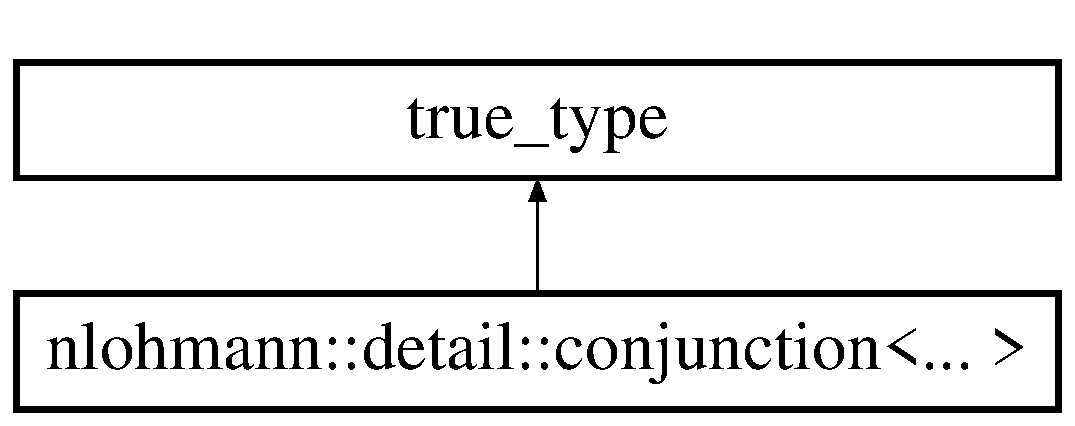
\includegraphics[height=2.000000cm]{dd/dde/structnlohmann_1_1detail_1_1conjunction}
\end{center}
\end{figure}


The documentation for this struct was generated from the following file\+:\begin{DoxyCompactItemize}
\item 
/home/mutzi/progs/linux\+\_\+workspace/alexa-\/avs-\/prototype/src/include/nlohmann\+\_\+json.\+h\end{DoxyCompactItemize}

\hypertarget{structnlohmann_1_1detail_1_1conjunction_3_01B1_01_4}{}\section{nlohmann\+:\+:detail\+:\+:conjunction$<$ B1 $>$ Struct Template Reference}
\label{structnlohmann_1_1detail_1_1conjunction_3_01B1_01_4}\index{nlohmann\+::detail\+::conjunction$<$ B1 $>$@{nlohmann\+::detail\+::conjunction$<$ B1 $>$}}
Inheritance diagram for nlohmann\+:\+:detail\+:\+:conjunction$<$ B1 $>$\+:\begin{figure}[H]
\begin{center}
\leavevmode
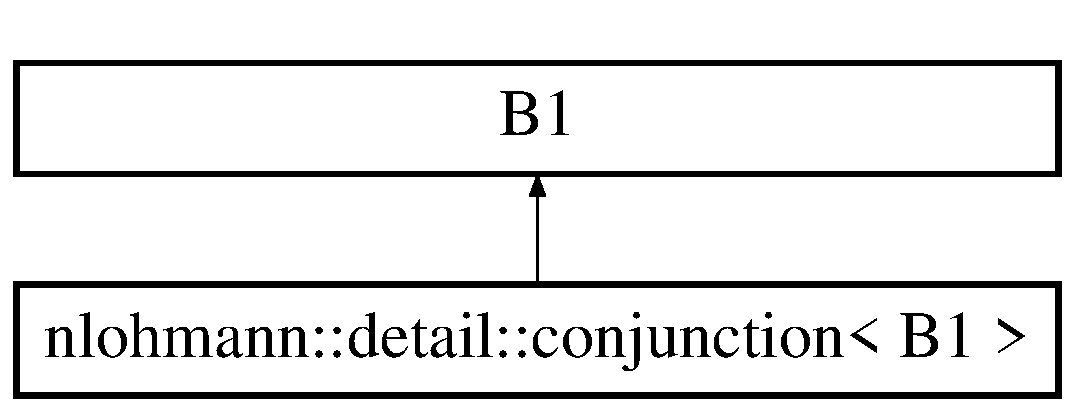
\includegraphics[height=2.000000cm]{d1/d96/structnlohmann_1_1detail_1_1conjunction_3_01B1_01_4}
\end{center}
\end{figure}


The documentation for this struct was generated from the following file\+:\begin{DoxyCompactItemize}
\item 
/home/mutzi/progs/linux\+\_\+workspace/alexa-\/avs-\/prototype/src/include/nlohmann\+\_\+json.\+h\end{DoxyCompactItemize}

\hypertarget{structnlohmann_1_1detail_1_1conjunction_3_01B1_00_01Bn_8_8_8_01_4}{}\section{nlohmann\+:\+:detail\+:\+:conjunction$<$ B1, Bn... $>$ Struct Template Reference}
\label{structnlohmann_1_1detail_1_1conjunction_3_01B1_00_01Bn_8_8_8_01_4}\index{nlohmann\+::detail\+::conjunction$<$ B1, Bn... $>$@{nlohmann\+::detail\+::conjunction$<$ B1, Bn... $>$}}
Inheritance diagram for nlohmann\+:\+:detail\+:\+:conjunction$<$ B1, Bn... $>$\+:\begin{figure}[H]
\begin{center}
\leavevmode
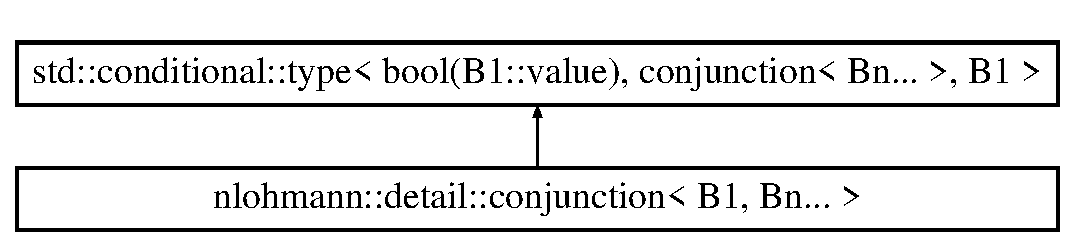
\includegraphics[height=2.000000cm]{d5/db0/structnlohmann_1_1detail_1_1conjunction_3_01B1_00_01Bn_8_8_8_01_4}
\end{center}
\end{figure}


The documentation for this struct was generated from the following file\+:\begin{DoxyCompactItemize}
\item 
/home/mutzi/progs/linux\+\_\+workspace/alexa-\/avs-\/prototype/src/include/nlohmann\+\_\+json.\+h\end{DoxyCompactItemize}

\hypertarget{structNetwork_1_1HTTP2_1_1DIRECTIVE__BYTES}{}\section{Network\+:\+:H\+T\+T\+P2\+:\+:D\+I\+R\+E\+C\+T\+I\+V\+E\+\_\+\+B\+Y\+T\+ES Struct Reference}
\label{structNetwork_1_1HTTP2_1_1DIRECTIVE__BYTES}\index{Network\+::\+H\+T\+T\+P2\+::\+D\+I\+R\+E\+C\+T\+I\+V\+E\+\_\+\+B\+Y\+T\+ES@{Network\+::\+H\+T\+T\+P2\+::\+D\+I\+R\+E\+C\+T\+I\+V\+E\+\_\+\+B\+Y\+T\+ES}}
\subsection*{Public Attributes}
\begin{DoxyCompactItemize}
\item 
\mbox{\Hypertarget{structNetwork_1_1HTTP2_1_1DIRECTIVE__BYTES_a28f7d91f0d3da806b49e2a501423cc92}\label{structNetwork_1_1HTTP2_1_1DIRECTIVE__BYTES_a28f7d91f0d3da806b49e2a501423cc92}} 
char $\ast$ {\bfseries bytes}
\item 
\mbox{\Hypertarget{structNetwork_1_1HTTP2_1_1DIRECTIVE__BYTES_a0074bf6ebab3ed9493ac7806c9dd2b8d}\label{structNetwork_1_1HTTP2_1_1DIRECTIVE__BYTES_a0074bf6ebab3ed9493ac7806c9dd2b8d}} 
size\+\_\+t {\bfseries size}
\end{DoxyCompactItemize}


The documentation for this struct was generated from the following file\+:\begin{DoxyCompactItemize}
\item 
/home/mutzi/progs/linux\+\_\+workspace/alexa-\/avs-\/prototype/src/include/http2multipartanalyse.\+h\end{DoxyCompactItemize}

\hypertarget{classNetwork_1_1HTTP_1_1DirectivenListener}{}\section{Network\+:\+:H\+T\+TP\+:\+:Directiven\+Listener Class Reference}
\label{classNetwork_1_1HTTP_1_1DirectivenListener}\index{Network\+::\+H\+T\+T\+P\+::\+Directiven\+Listener@{Network\+::\+H\+T\+T\+P\+::\+Directiven\+Listener}}
Inheritance diagram for Network\+:\+:H\+T\+TP\+:\+:Directiven\+Listener\+:\begin{figure}[H]
\begin{center}
\leavevmode
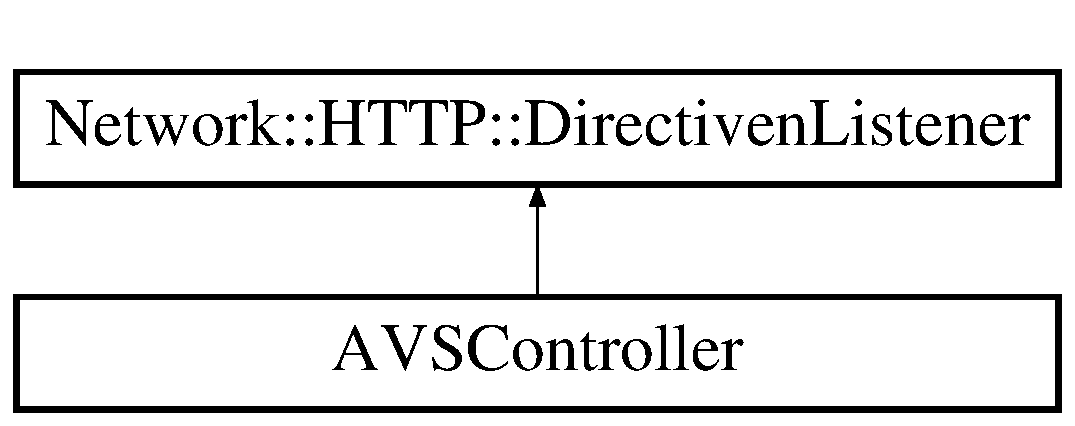
\includegraphics[height=2.000000cm]{dd/d01/classNetwork_1_1HTTP_1_1DirectivenListener}
\end{center}
\end{figure}
\subsection*{Public Member Functions}
\begin{DoxyCompactItemize}
\item 
\mbox{\Hypertarget{classNetwork_1_1HTTP_1_1DirectivenListener_a7bee132b3a6e4627a6f867af38df6a2a}\label{classNetwork_1_1HTTP_1_1DirectivenListener_a7bee132b3a6e4627a6f867af38df6a2a}} 
virtual void {\bfseries on\+Speech\+Synthesizer\+Speak\+Directive} (const \hyperlink{classNetwork_1_1HTTP_1_1HTTPClientDirectiveEvent}{H\+T\+T\+P\+Client\+Directive\+Event} $\ast$event)=0
\item 
\mbox{\Hypertarget{classNetwork_1_1HTTP_1_1DirectivenListener_a85b39ee362f07c68a066ce787c8d7430}\label{classNetwork_1_1HTTP_1_1DirectivenListener_a85b39ee362f07c68a066ce787c8d7430}} 
virtual void {\bfseries on\+Speech\+Recognize\+Stop\+Capture\+Directive} (const \hyperlink{classNetwork_1_1HTTP_1_1HTTPClientDirectiveEvent}{H\+T\+T\+P\+Client\+Directive\+Event} $\ast$event)=0
\item 
\mbox{\Hypertarget{classNetwork_1_1HTTP_1_1DirectivenListener_af0ad2595a831168a5a783ac857e3d3e2}\label{classNetwork_1_1HTTP_1_1DirectivenListener_af0ad2595a831168a5a783ac857e3d3e2}} 
virtual void {\bfseries on\+Speech\+Recognize\+Expect\+Speech\+Directive} (const \hyperlink{classNetwork_1_1HTTP_1_1HTTPClientDirectiveEvent}{H\+T\+T\+P\+Client\+Directive\+Event} $\ast$event)=0
\item 
\mbox{\Hypertarget{classNetwork_1_1HTTP_1_1DirectivenListener_a2dba0d0b3f2ccf34eed83f8f7bb8973f}\label{classNetwork_1_1HTTP_1_1DirectivenListener_a2dba0d0b3f2ccf34eed83f8f7bb8973f}} 
virtual void {\bfseries on\+Speeker\+Set\+Mute\+Directive} (const \hyperlink{classNetwork_1_1HTTP_1_1HTTPClientDirectiveEvent}{H\+T\+T\+P\+Client\+Directive\+Event} $\ast$event)=0
\end{DoxyCompactItemize}


The documentation for this class was generated from the following file\+:\begin{DoxyCompactItemize}
\item 
/home/mutzi/progs/linux\+\_\+workspace/alexa-\/avs-\/prototype/src/include/directivenlistener.\+h\end{DoxyCompactItemize}

\hypertarget{structErrorException}{}\section{Error\+Exception Struct Reference}
\label{structErrorException}\index{Error\+Exception@{Error\+Exception}}
Inheritance diagram for Error\+Exception\+:\begin{figure}[H]
\begin{center}
\leavevmode
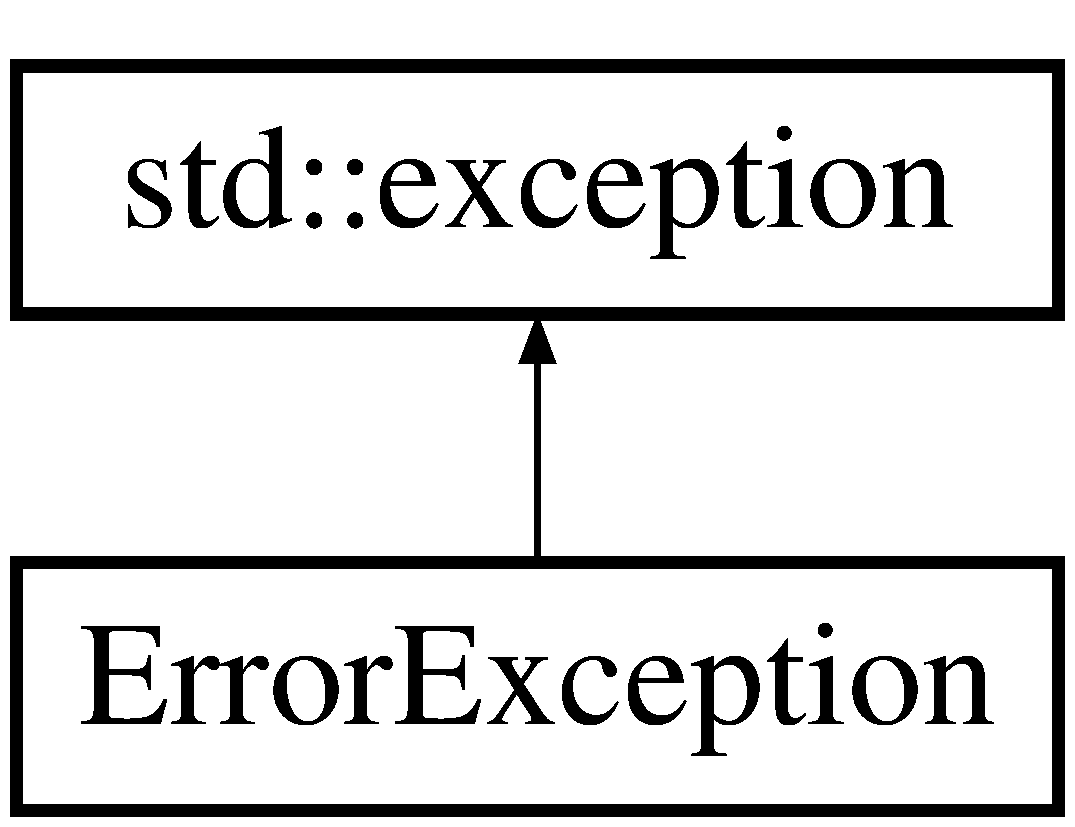
\includegraphics[height=2.000000cm]{df/d85/structErrorException}
\end{center}
\end{figure}
\subsection*{Public Member Functions}
\begin{DoxyCompactItemize}
\item 
\mbox{\Hypertarget{structErrorException_a6de4ce56ef8944558d91c6d3d229620e}\label{structErrorException_a6de4ce56ef8944558d91c6d3d229620e}} 
{\bfseries Error\+Exception} (std\+::string ss)
\item 
\mbox{\Hypertarget{structErrorException_a9cee101d4140d24592c243496110a1b2}\label{structErrorException_a9cee101d4140d24592c243496110a1b2}} 
{\bfseries Error\+Exception} (std\+::string ss, const char $\ast$c\+\_\+ss)
\item 
\mbox{\Hypertarget{structErrorException_a2f53b316b322c7a5b6361de7179f8a3b}\label{structErrorException_a2f53b316b322c7a5b6361de7179f8a3b}} 
const char $\ast$ {\bfseries what} () const  throw ()
\end{DoxyCompactItemize}
\subsection*{Public Attributes}
\begin{DoxyCompactItemize}
\item 
\mbox{\Hypertarget{structErrorException_ad24d7aec3e1e273c8c9e18e3d4ca0571}\label{structErrorException_ad24d7aec3e1e273c8c9e18e3d4ca0571}} 
std\+::string {\bfseries s}
\end{DoxyCompactItemize}


The documentation for this struct was generated from the following file\+:\begin{DoxyCompactItemize}
\item 
/home/mutzi/progs/linux\+\_\+workspace/alexa-\/avs-\/prototype/src/include/stdafx.\+h\end{DoxyCompactItemize}

\hypertarget{classnlohmann_1_1detail_1_1exception}{}\section{nlohmann\+:\+:detail\+:\+:exception Class Reference}
\label{classnlohmann_1_1detail_1_1exception}\index{nlohmann\+::detail\+::exception@{nlohmann\+::detail\+::exception}}


general exception of the \hyperlink{classnlohmann_1_1basic__json}{basic\+\_\+json} class  




{\ttfamily \#include $<$nlohmann\+\_\+json.\+h$>$}

Inheritance diagram for nlohmann\+:\+:detail\+:\+:exception\+:\begin{figure}[H]
\begin{center}
\leavevmode
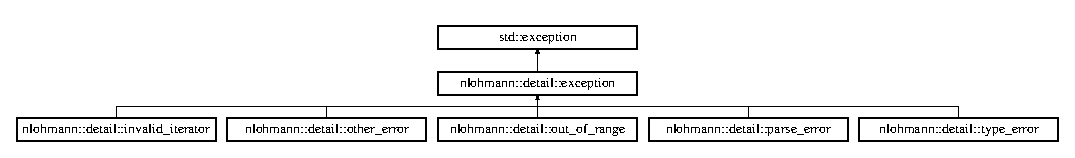
\includegraphics[height=1.680000cm]{de/df2/classnlohmann_1_1detail_1_1exception}
\end{center}
\end{figure}
\subsection*{Public Member Functions}
\begin{DoxyCompactItemize}
\item 
\mbox{\Hypertarget{classnlohmann_1_1detail_1_1exception_a86b7eaa74e0b2d645bf399be693237ac}\label{classnlohmann_1_1detail_1_1exception_a86b7eaa74e0b2d645bf399be693237ac}} 
virtual const char $\ast$ \hyperlink{classnlohmann_1_1detail_1_1exception_a86b7eaa74e0b2d645bf399be693237ac}{what} () const noexcept override
\begin{DoxyCompactList}\small\item\em returns the explanatory string \end{DoxyCompactList}\end{DoxyCompactItemize}
\subsection*{Public Attributes}
\begin{DoxyCompactItemize}
\item 
\mbox{\Hypertarget{classnlohmann_1_1detail_1_1exception_a0d4589a3fb54e81646d986c05efa3b9a}\label{classnlohmann_1_1detail_1_1exception_a0d4589a3fb54e81646d986c05efa3b9a}} 
const int \hyperlink{classnlohmann_1_1detail_1_1exception_a0d4589a3fb54e81646d986c05efa3b9a}{id}
\begin{DoxyCompactList}\small\item\em the id of the exception \end{DoxyCompactList}\end{DoxyCompactItemize}
\subsection*{Protected Member Functions}
\begin{DoxyCompactItemize}
\item 
\mbox{\Hypertarget{classnlohmann_1_1detail_1_1exception_ae323ad0d53bc724414c2233164e65657}\label{classnlohmann_1_1detail_1_1exception_ae323ad0d53bc724414c2233164e65657}} 
{\bfseries exception} (int id\+\_\+, const char $\ast$what\+\_\+arg)
\end{DoxyCompactItemize}
\subsection*{Static Protected Member Functions}
\begin{DoxyCompactItemize}
\item 
\mbox{\Hypertarget{classnlohmann_1_1detail_1_1exception_aac7455bbbaed7c01ecd5a2ead336b1ae}\label{classnlohmann_1_1detail_1_1exception_aac7455bbbaed7c01ecd5a2ead336b1ae}} 
static \hyperlink{namespacenlohmann_1_1detail_a90aa5ef615aa8305e9ea20d8a947980fab45cffe084dd3d20d928bee85e7b0f21}{std\+::string} {\bfseries name} (const \hyperlink{namespacenlohmann_1_1detail_a90aa5ef615aa8305e9ea20d8a947980fab45cffe084dd3d20d928bee85e7b0f21}{std\+::string} \&ename, int \hyperlink{classnlohmann_1_1detail_1_1exception_a0d4589a3fb54e81646d986c05efa3b9a}{id})
\end{DoxyCompactItemize}


\subsection{Detailed Description}
general exception of the \hyperlink{classnlohmann_1_1basic__json}{basic\+\_\+json} class 

Extension of std\+::exception objects with a member {\itshape id} for exception ids.

\begin{DoxyNote}{Note}
To have nothrow-\/copy-\/constructible exceptions, we internally use std\+::runtime\+\_\+error which can cope with arbitrary-\/length error messages. Intermediate strings are built with static functions and then passed to the actual constructor.
\end{DoxyNote}
\begin{DoxySince}{Since}
version 3.\+0.\+0 
\end{DoxySince}


The documentation for this class was generated from the following file\+:\begin{DoxyCompactItemize}
\item 
/home/mutzi/progs/linux\+\_\+workspace/alexa-\/avs-\/prototype/src/include/nlohmann\+\_\+json.\+h\end{DoxyCompactItemize}

\hypertarget{structnlohmann_1_1detail_1_1external__constructor}{}\section{nlohmann\+:\+:detail\+:\+:external\+\_\+constructor$<$ value\+\_\+t $>$ Struct Template Reference}
\label{structnlohmann_1_1detail_1_1external__constructor}\index{nlohmann\+::detail\+::external\+\_\+constructor$<$ value\+\_\+t $>$@{nlohmann\+::detail\+::external\+\_\+constructor$<$ value\+\_\+t $>$}}


The documentation for this struct was generated from the following file\+:\begin{DoxyCompactItemize}
\item 
/home/mutzi/progs/linux\+\_\+workspace/alexa-\/avs-\/prototype/src/include/nlohmann\+\_\+json.\+h\end{DoxyCompactItemize}

\hypertarget{structnlohmann_1_1detail_1_1external__constructor_3_01value__t_1_1array_01_4}{}\section{nlohmann\+:\+:detail\+:\+:external\+\_\+constructor$<$ value\+\_\+t\+:\+:array $>$ Struct Template Reference}
\label{structnlohmann_1_1detail_1_1external__constructor_3_01value__t_1_1array_01_4}\index{nlohmann\+::detail\+::external\+\_\+constructor$<$ value\+\_\+t\+::array $>$@{nlohmann\+::detail\+::external\+\_\+constructor$<$ value\+\_\+t\+::array $>$}}
\subsection*{Static Public Member Functions}
\begin{DoxyCompactItemize}
\item 
\mbox{\Hypertarget{structnlohmann_1_1detail_1_1external__constructor_3_01value__t_1_1array_01_4_abfb2a6eec0bc21e8a7438546aebc55d8}\label{structnlohmann_1_1detail_1_1external__constructor_3_01value__t_1_1array_01_4_abfb2a6eec0bc21e8a7438546aebc55d8}} 
{\footnotesize template$<$typename Basic\+Json\+Type $>$ }\\static void {\bfseries construct} (Basic\+Json\+Type \&j, const typename Basic\+Json\+Type\+::array\+\_\+t \&arr)
\item 
\mbox{\Hypertarget{structnlohmann_1_1detail_1_1external__constructor_3_01value__t_1_1array_01_4_a110f50fd5378da876d9a6d6a8d945e37}\label{structnlohmann_1_1detail_1_1external__constructor_3_01value__t_1_1array_01_4_a110f50fd5378da876d9a6d6a8d945e37}} 
{\footnotesize template$<$typename Basic\+Json\+Type , typename Compatible\+Array\+Type , enable\+\_\+if\+\_\+t$<$ not std\+::is\+\_\+same$<$ Compatible\+Array\+Type, typename Basic\+Json\+Type\+::array\+\_\+t $>$\+::value, int $>$  = 0$>$ }\\static void {\bfseries construct} (Basic\+Json\+Type \&j, const Compatible\+Array\+Type \&arr)
\item 
\mbox{\Hypertarget{structnlohmann_1_1detail_1_1external__constructor_3_01value__t_1_1array_01_4_a4ebb19b1cb84b4cb224a4c5322e16f14}\label{structnlohmann_1_1detail_1_1external__constructor_3_01value__t_1_1array_01_4_a4ebb19b1cb84b4cb224a4c5322e16f14}} 
{\footnotesize template$<$typename Basic\+Json\+Type $>$ }\\static void {\bfseries construct} (Basic\+Json\+Type \&j, const std\+::vector$<$ bool $>$ \&arr)
\end{DoxyCompactItemize}


The documentation for this struct was generated from the following file\+:\begin{DoxyCompactItemize}
\item 
/home/mutzi/progs/linux\+\_\+workspace/alexa-\/avs-\/prototype/src/include/nlohmann\+\_\+json.\+h\end{DoxyCompactItemize}

\hypertarget{structnlohmann_1_1detail_1_1external__constructor_3_01value__t_1_1boolean_01_4}{}\section{nlohmann\+:\+:detail\+:\+:external\+\_\+constructor$<$ value\+\_\+t\+:\+:boolean $>$ Struct Template Reference}
\label{structnlohmann_1_1detail_1_1external__constructor_3_01value__t_1_1boolean_01_4}\index{nlohmann\+::detail\+::external\+\_\+constructor$<$ value\+\_\+t\+::boolean $>$@{nlohmann\+::detail\+::external\+\_\+constructor$<$ value\+\_\+t\+::boolean $>$}}
\subsection*{Static Public Member Functions}
\begin{DoxyCompactItemize}
\item 
\mbox{\Hypertarget{structnlohmann_1_1detail_1_1external__constructor_3_01value__t_1_1boolean_01_4_a867122bcf0856c757bd6bcbfb8be74bc}\label{structnlohmann_1_1detail_1_1external__constructor_3_01value__t_1_1boolean_01_4_a867122bcf0856c757bd6bcbfb8be74bc}} 
{\footnotesize template$<$typename Basic\+Json\+Type $>$ }\\static void {\bfseries construct} (Basic\+Json\+Type \&j, typename Basic\+Json\+Type\+::boolean\+\_\+t b) noexcept
\end{DoxyCompactItemize}


The documentation for this struct was generated from the following file\+:\begin{DoxyCompactItemize}
\item 
/home/mutzi/progs/linux\+\_\+workspace/alexa-\/avs-\/prototype/src/include/nlohmann\+\_\+json.\+h\end{DoxyCompactItemize}

\hypertarget{structnlohmann_1_1detail_1_1external__constructor_3_01value__t_1_1number__float_01_4}{}\section{nlohmann\+:\+:detail\+:\+:external\+\_\+constructor$<$ value\+\_\+t\+:\+:number\+\_\+float $>$ Struct Template Reference}
\label{structnlohmann_1_1detail_1_1external__constructor_3_01value__t_1_1number__float_01_4}\index{nlohmann\+::detail\+::external\+\_\+constructor$<$ value\+\_\+t\+::number\+\_\+float $>$@{nlohmann\+::detail\+::external\+\_\+constructor$<$ value\+\_\+t\+::number\+\_\+float $>$}}
\subsection*{Static Public Member Functions}
\begin{DoxyCompactItemize}
\item 
\mbox{\Hypertarget{structnlohmann_1_1detail_1_1external__constructor_3_01value__t_1_1number__float_01_4_a669df5a4d258b588e67f747c6d656cdb}\label{structnlohmann_1_1detail_1_1external__constructor_3_01value__t_1_1number__float_01_4_a669df5a4d258b588e67f747c6d656cdb}} 
{\footnotesize template$<$typename Basic\+Json\+Type $>$ }\\static void {\bfseries construct} (Basic\+Json\+Type \&j, typename Basic\+Json\+Type\+::number\+\_\+float\+\_\+t val) noexcept
\end{DoxyCompactItemize}


The documentation for this struct was generated from the following file\+:\begin{DoxyCompactItemize}
\item 
/home/mutzi/progs/linux\+\_\+workspace/alexa-\/avs-\/prototype/src/include/nlohmann\+\_\+json.\+h\end{DoxyCompactItemize}

\hypertarget{structnlohmann_1_1detail_1_1external__constructor_3_01value__t_1_1number__integer_01_4}{}\section{nlohmann\+:\+:detail\+:\+:external\+\_\+constructor$<$ value\+\_\+t\+:\+:number\+\_\+integer $>$ Struct Template Reference}
\label{structnlohmann_1_1detail_1_1external__constructor_3_01value__t_1_1number__integer_01_4}\index{nlohmann\+::detail\+::external\+\_\+constructor$<$ value\+\_\+t\+::number\+\_\+integer $>$@{nlohmann\+::detail\+::external\+\_\+constructor$<$ value\+\_\+t\+::number\+\_\+integer $>$}}
\subsection*{Static Public Member Functions}
\begin{DoxyCompactItemize}
\item 
\mbox{\Hypertarget{structnlohmann_1_1detail_1_1external__constructor_3_01value__t_1_1number__integer_01_4_a7c3949672ddb45095cc2527635feef0b}\label{structnlohmann_1_1detail_1_1external__constructor_3_01value__t_1_1number__integer_01_4_a7c3949672ddb45095cc2527635feef0b}} 
{\footnotesize template$<$typename Basic\+Json\+Type $>$ }\\static void {\bfseries construct} (Basic\+Json\+Type \&j, typename Basic\+Json\+Type\+::number\+\_\+integer\+\_\+t val) noexcept
\end{DoxyCompactItemize}


The documentation for this struct was generated from the following file\+:\begin{DoxyCompactItemize}
\item 
/home/mutzi/progs/linux\+\_\+workspace/alexa-\/avs-\/prototype/src/include/nlohmann\+\_\+json.\+h\end{DoxyCompactItemize}

\hypertarget{structnlohmann_1_1detail_1_1external__constructor_3_01value__t_1_1number__unsigned_01_4}{}\section{nlohmann\+:\+:detail\+:\+:external\+\_\+constructor$<$ value\+\_\+t\+:\+:number\+\_\+unsigned $>$ Struct Template Reference}
\label{structnlohmann_1_1detail_1_1external__constructor_3_01value__t_1_1number__unsigned_01_4}\index{nlohmann\+::detail\+::external\+\_\+constructor$<$ value\+\_\+t\+::number\+\_\+unsigned $>$@{nlohmann\+::detail\+::external\+\_\+constructor$<$ value\+\_\+t\+::number\+\_\+unsigned $>$}}
\subsection*{Static Public Member Functions}
\begin{DoxyCompactItemize}
\item 
\mbox{\Hypertarget{structnlohmann_1_1detail_1_1external__constructor_3_01value__t_1_1number__unsigned_01_4_a17969b14852f43e04353858c87b0f539}\label{structnlohmann_1_1detail_1_1external__constructor_3_01value__t_1_1number__unsigned_01_4_a17969b14852f43e04353858c87b0f539}} 
{\footnotesize template$<$typename Basic\+Json\+Type $>$ }\\static void {\bfseries construct} (Basic\+Json\+Type \&j, typename Basic\+Json\+Type\+::number\+\_\+unsigned\+\_\+t val) noexcept
\end{DoxyCompactItemize}


The documentation for this struct was generated from the following file\+:\begin{DoxyCompactItemize}
\item 
/home/mutzi/progs/linux\+\_\+workspace/alexa-\/avs-\/prototype/src/include/nlohmann\+\_\+json.\+h\end{DoxyCompactItemize}

\hypertarget{structnlohmann_1_1detail_1_1external__constructor_3_01value__t_1_1object_01_4}{}\section{nlohmann\+:\+:detail\+:\+:external\+\_\+constructor$<$ value\+\_\+t\+:\+:object $>$ Struct Template Reference}
\label{structnlohmann_1_1detail_1_1external__constructor_3_01value__t_1_1object_01_4}\index{nlohmann\+::detail\+::external\+\_\+constructor$<$ value\+\_\+t\+::object $>$@{nlohmann\+::detail\+::external\+\_\+constructor$<$ value\+\_\+t\+::object $>$}}
\subsection*{Static Public Member Functions}
\begin{DoxyCompactItemize}
\item 
\mbox{\Hypertarget{structnlohmann_1_1detail_1_1external__constructor_3_01value__t_1_1object_01_4_a3a369c5d49596dd4411e368425f9ac7a}\label{structnlohmann_1_1detail_1_1external__constructor_3_01value__t_1_1object_01_4_a3a369c5d49596dd4411e368425f9ac7a}} 
{\footnotesize template$<$typename Basic\+Json\+Type $>$ }\\static void {\bfseries construct} (Basic\+Json\+Type \&j, const typename Basic\+Json\+Type\+::object\+\_\+t \&obj)
\item 
\mbox{\Hypertarget{structnlohmann_1_1detail_1_1external__constructor_3_01value__t_1_1object_01_4_a91f89abe0ec4dec59099b691682ff927}\label{structnlohmann_1_1detail_1_1external__constructor_3_01value__t_1_1object_01_4_a91f89abe0ec4dec59099b691682ff927}} 
{\footnotesize template$<$typename Basic\+Json\+Type , typename Compatible\+Object\+Type , enable\+\_\+if\+\_\+t$<$ not std\+::is\+\_\+same$<$ Compatible\+Object\+Type, typename Basic\+Json\+Type\+::object\+\_\+t $>$\+::value, int $>$  = 0$>$ }\\static void {\bfseries construct} (Basic\+Json\+Type \&j, const Compatible\+Object\+Type \&obj)
\end{DoxyCompactItemize}


The documentation for this struct was generated from the following file\+:\begin{DoxyCompactItemize}
\item 
/home/mutzi/progs/linux\+\_\+workspace/alexa-\/avs-\/prototype/src/include/nlohmann\+\_\+json.\+h\end{DoxyCompactItemize}

\hypertarget{structnlohmann_1_1detail_1_1external__constructor_3_01value__t_1_1string_01_4}{}\section{nlohmann\+:\+:detail\+:\+:external\+\_\+constructor$<$ value\+\_\+t\+:\+:string $>$ Struct Template Reference}
\label{structnlohmann_1_1detail_1_1external__constructor_3_01value__t_1_1string_01_4}\index{nlohmann\+::detail\+::external\+\_\+constructor$<$ value\+\_\+t\+::string $>$@{nlohmann\+::detail\+::external\+\_\+constructor$<$ value\+\_\+t\+::string $>$}}
\subsection*{Static Public Member Functions}
\begin{DoxyCompactItemize}
\item 
\mbox{\Hypertarget{structnlohmann_1_1detail_1_1external__constructor_3_01value__t_1_1string_01_4_ad88d0b4b7ea01ea20e12cc1b82fe0d92}\label{structnlohmann_1_1detail_1_1external__constructor_3_01value__t_1_1string_01_4_ad88d0b4b7ea01ea20e12cc1b82fe0d92}} 
{\footnotesize template$<$typename Basic\+Json\+Type $>$ }\\static void {\bfseries construct} (Basic\+Json\+Type \&j, const typename Basic\+Json\+Type\+::string\+\_\+t \&s)
\end{DoxyCompactItemize}


The documentation for this struct was generated from the following file\+:\begin{DoxyCompactItemize}
\item 
/home/mutzi/progs/linux\+\_\+workspace/alexa-\/avs-\/prototype/src/include/nlohmann\+\_\+json.\+h\end{DoxyCompactItemize}

\hypertarget{structFileBytes}{}\section{File\+Bytes Struct Reference}
\label{structFileBytes}\index{File\+Bytes@{File\+Bytes}}
\subsection*{Public Attributes}
\begin{DoxyCompactItemize}
\item 
\mbox{\Hypertarget{structFileBytes_a1a32b326061286eb4d7551efb950c2fb}\label{structFileBytes_a1a32b326061286eb4d7551efb950c2fb}} 
char $\ast$ {\bfseries bytes}
\item 
\mbox{\Hypertarget{structFileBytes_a604b8d5fde88eb710f085717627a3953}\label{structFileBytes_a604b8d5fde88eb710f085717627a3953}} 
size\+\_\+t {\bfseries size}
\end{DoxyCompactItemize}


The documentation for this struct was generated from the following file\+:\begin{DoxyCompactItemize}
\item 
/home/mutzi/progs/linux\+\_\+workspace/alexa-\/avs-\/prototype/src/include/bytefileloader.\+h\end{DoxyCompactItemize}

\hypertarget{classFileLoader}{}\section{File\+Loader Class Reference}
\label{classFileLoader}\index{File\+Loader@{File\+Loader}}
Inheritance diagram for File\+Loader\+:\begin{figure}[H]
\begin{center}
\leavevmode
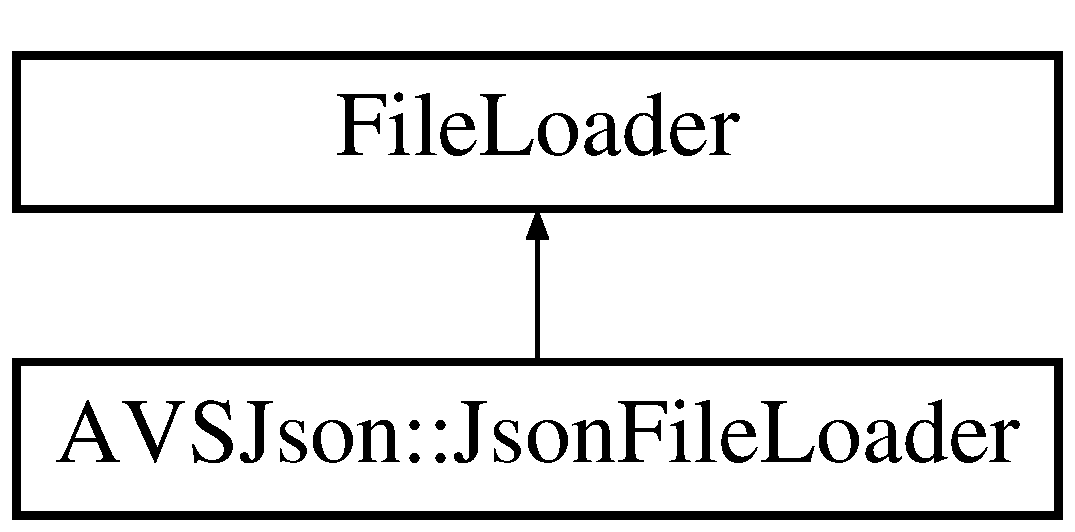
\includegraphics[height=2.000000cm]{d6/dc2/classFileLoader}
\end{center}
\end{figure}
\subsection*{Public Member Functions}
\begin{DoxyCompactItemize}
\item 
\mbox{\Hypertarget{classFileLoader_acf79b58743d2cbe7ff9cfb7dbd9d0f41}\label{classFileLoader_acf79b58743d2cbe7ff9cfb7dbd9d0f41}} 
{\bfseries File\+Loader} (const std\+::string file\+\_\+name)
\item 
\mbox{\Hypertarget{classFileLoader_aad27b1e65065793fe7329c7a4748c1ec}\label{classFileLoader_aad27b1e65065793fe7329c7a4748c1ec}} 
void {\bfseries set\+File\+Name} (const std\+::string file\+\_\+name)
\item 
\mbox{\Hypertarget{classFileLoader_aea473d22b9d3da6c60bd4da463cb29b6}\label{classFileLoader_aea473d22b9d3da6c60bd4da463cb29b6}} 
void {\bfseries load} ()
\item 
\mbox{\Hypertarget{classFileLoader_af70b4c26a019ca0b3aca1e62cf894a8a}\label{classFileLoader_af70b4c26a019ca0b3aca1e62cf894a8a}} 
virtual void {\bfseries on\+Line\+Event} (const std\+::string line)=0
\item 
\mbox{\Hypertarget{classFileLoader_aea70e4f31438f22dfb37b18793269299}\label{classFileLoader_aea70e4f31438f22dfb37b18793269299}} 
virtual void {\bfseries on\+End\+Of\+File\+Event} (void)=0
\item 
\mbox{\Hypertarget{classFileLoader_a7843d56d0d1c5238b886180a154c43e9}\label{classFileLoader_a7843d56d0d1c5238b886180a154c43e9}} 
void {\bfseries replace\+All} (std\+::string \&input, std\+::string search, std\+::string replace)
\item 
\mbox{\Hypertarget{classFileLoader_a587614f144fa4791a61a769a28644aca}\label{classFileLoader_a587614f144fa4791a61a769a28644aca}} 
std\+::string {\bfseries convert\+To} (long number)
\item 
\mbox{\Hypertarget{classFileLoader_a9f8050d7d81f4974c1e7e14c0a082b25}\label{classFileLoader_a9f8050d7d81f4974c1e7e14c0a082b25}} 
std\+::string {\bfseries convert\+To} (bool boolean)
\end{DoxyCompactItemize}


The documentation for this class was generated from the following files\+:\begin{DoxyCompactItemize}
\item 
/home/mutzi/progs/linux\+\_\+workspace/alexa-\/avs-\/prototype/src/include/fileloader.\+h\item 
/home/mutzi/progs/linux\+\_\+workspace/alexa-\/avs-\/prototype/src/fileloader.\+cpp\end{DoxyCompactItemize}

\hypertarget{structnlohmann_1_1detail_1_1from__json__fn}{}\section{nlohmann\+:\+:detail\+:\+:from\+\_\+json\+\_\+fn Struct Reference}
\label{structnlohmann_1_1detail_1_1from__json__fn}\index{nlohmann\+::detail\+::from\+\_\+json\+\_\+fn@{nlohmann\+::detail\+::from\+\_\+json\+\_\+fn}}
\subsection*{Public Member Functions}
\begin{DoxyCompactItemize}
\item 
\mbox{\Hypertarget{structnlohmann_1_1detail_1_1from__json__fn_a48e82ad9d244fdf249caa970a253e214}\label{structnlohmann_1_1detail_1_1from__json__fn_a48e82ad9d244fdf249caa970a253e214}} 
{\footnotesize template$<$typename Basic\+Json\+Type , typename T $>$ }\\void {\bfseries operator()} (const Basic\+Json\+Type \&j, T \&val) const noexcept(noexcept(std\+::declval$<$ \hyperlink{structnlohmann_1_1detail_1_1from__json__fn}{from\+\_\+json\+\_\+fn} $>$().call(j, val, \hyperlink{structnlohmann_1_1detail_1_1priority__tag}{priority\+\_\+tag}$<$ 1 $>$ \{\})))
\end{DoxyCompactItemize}


The documentation for this struct was generated from the following file\+:\begin{DoxyCompactItemize}
\item 
/home/mutzi/progs/linux\+\_\+workspace/alexa-\/avs-\/prototype/src/include/nlohmann\+\_\+json.\+h\end{DoxyCompactItemize}

\hypertarget{structnlohmann_1_1detail_1_1has__from__json}{}\section{nlohmann\+:\+:detail\+:\+:has\+\_\+from\+\_\+json$<$ Basic\+Json\+Type, T $>$ Struct Template Reference}
\label{structnlohmann_1_1detail_1_1has__from__json}\index{nlohmann\+::detail\+::has\+\_\+from\+\_\+json$<$ Basic\+Json\+Type, T $>$@{nlohmann\+::detail\+::has\+\_\+from\+\_\+json$<$ Basic\+Json\+Type, T $>$}}
\subsection*{Static Public Attributes}
\begin{DoxyCompactItemize}
\item 
static constexpr bool {\bfseries value}
\end{DoxyCompactItemize}


\subsection{Member Data Documentation}
\mbox{\Hypertarget{structnlohmann_1_1detail_1_1has__from__json_a16701d806343c58ae7e884024dd14955}\label{structnlohmann_1_1detail_1_1has__from__json_a16701d806343c58ae7e884024dd14955}} 
\index{nlohmann\+::detail\+::has\+\_\+from\+\_\+json@{nlohmann\+::detail\+::has\+\_\+from\+\_\+json}!value@{value}}
\index{value@{value}!nlohmann\+::detail\+::has\+\_\+from\+\_\+json@{nlohmann\+::detail\+::has\+\_\+from\+\_\+json}}
\subsubsection{\texorpdfstring{value}{value}}
{\footnotesize\ttfamily template$<$typename Basic\+Json\+Type , typename T $>$ \\
constexpr bool \hyperlink{structnlohmann_1_1detail_1_1has__from__json}{nlohmann\+::detail\+::has\+\_\+from\+\_\+json}$<$ Basic\+Json\+Type, T $>$\+::value\hspace{0.3cm}{\ttfamily [static]}}

{\bfseries Initial value\+:}
\begin{DoxyCode}
= std::is\_integral<decltype(
                                      detect(std::declval<\textcolor{keyword}{typename} BasicJsonType::template 
      json\_serializer<T, void>>()))>::value
\end{DoxyCode}


The documentation for this struct was generated from the following file\+:\begin{DoxyCompactItemize}
\item 
/home/mutzi/progs/linux\+\_\+workspace/alexa-\/avs-\/prototype/src/include/nlohmann\+\_\+json.\+h\end{DoxyCompactItemize}

\hypertarget{structnlohmann_1_1detail_1_1has__non__default__from__json}{}\section{nlohmann\+:\+:detail\+:\+:has\+\_\+non\+\_\+default\+\_\+from\+\_\+json$<$ Basic\+Json\+Type, T $>$ Struct Template Reference}
\label{structnlohmann_1_1detail_1_1has__non__default__from__json}\index{nlohmann\+::detail\+::has\+\_\+non\+\_\+default\+\_\+from\+\_\+json$<$ Basic\+Json\+Type, T $>$@{nlohmann\+::detail\+::has\+\_\+non\+\_\+default\+\_\+from\+\_\+json$<$ Basic\+Json\+Type, T $>$}}
\subsection*{Static Public Attributes}
\begin{DoxyCompactItemize}
\item 
static constexpr bool {\bfseries value}
\end{DoxyCompactItemize}


\subsection{Member Data Documentation}
\mbox{\Hypertarget{structnlohmann_1_1detail_1_1has__non__default__from__json_ad34bb7cd3961fcafc2c5047a9782e931}\label{structnlohmann_1_1detail_1_1has__non__default__from__json_ad34bb7cd3961fcafc2c5047a9782e931}} 
\index{nlohmann\+::detail\+::has\+\_\+non\+\_\+default\+\_\+from\+\_\+json@{nlohmann\+::detail\+::has\+\_\+non\+\_\+default\+\_\+from\+\_\+json}!value@{value}}
\index{value@{value}!nlohmann\+::detail\+::has\+\_\+non\+\_\+default\+\_\+from\+\_\+json@{nlohmann\+::detail\+::has\+\_\+non\+\_\+default\+\_\+from\+\_\+json}}
\subsubsection{\texorpdfstring{value}{value}}
{\footnotesize\ttfamily template$<$typename Basic\+Json\+Type , typename T $>$ \\
constexpr bool \hyperlink{structnlohmann_1_1detail_1_1has__non__default__from__json}{nlohmann\+::detail\+::has\+\_\+non\+\_\+default\+\_\+from\+\_\+json}$<$ Basic\+Json\+Type, T $>$\+::value\hspace{0.3cm}{\ttfamily [static]}}

{\bfseries Initial value\+:}
\begin{DoxyCode}
= std::is\_integral<decltype(detect(
                                      std::declval<\textcolor{keyword}{typename} BasicJsonType::template json\_serializer<T,
       void>>()))>::value
\end{DoxyCode}


The documentation for this struct was generated from the following file\+:\begin{DoxyCompactItemize}
\item 
/home/mutzi/progs/linux\+\_\+workspace/alexa-\/avs-\/prototype/src/include/nlohmann\+\_\+json.\+h\end{DoxyCompactItemize}

\hypertarget{structnlohmann_1_1detail_1_1has__to__json}{}\section{nlohmann\+:\+:detail\+:\+:has\+\_\+to\+\_\+json$<$ Basic\+Json\+Type, T $>$ Struct Template Reference}
\label{structnlohmann_1_1detail_1_1has__to__json}\index{nlohmann\+::detail\+::has\+\_\+to\+\_\+json$<$ Basic\+Json\+Type, T $>$@{nlohmann\+::detail\+::has\+\_\+to\+\_\+json$<$ Basic\+Json\+Type, T $>$}}
\subsection*{Static Public Attributes}
\begin{DoxyCompactItemize}
\item 
static constexpr bool {\bfseries value}
\end{DoxyCompactItemize}


\subsection{Member Data Documentation}
\mbox{\Hypertarget{structnlohmann_1_1detail_1_1has__to__json_a18e260c3c6f10328637c4427d3cb3a31}\label{structnlohmann_1_1detail_1_1has__to__json_a18e260c3c6f10328637c4427d3cb3a31}} 
\index{nlohmann\+::detail\+::has\+\_\+to\+\_\+json@{nlohmann\+::detail\+::has\+\_\+to\+\_\+json}!value@{value}}
\index{value@{value}!nlohmann\+::detail\+::has\+\_\+to\+\_\+json@{nlohmann\+::detail\+::has\+\_\+to\+\_\+json}}
\subsubsection{\texorpdfstring{value}{value}}
{\footnotesize\ttfamily template$<$typename Basic\+Json\+Type , typename T $>$ \\
constexpr bool \hyperlink{structnlohmann_1_1detail_1_1has__to__json}{nlohmann\+::detail\+::has\+\_\+to\+\_\+json}$<$ Basic\+Json\+Type, T $>$\+::value\hspace{0.3cm}{\ttfamily [static]}}

{\bfseries Initial value\+:}
\begin{DoxyCode}
= std::is\_integral<decltype(detect(
                                      std::declval<\textcolor{keyword}{typename} BasicJsonType::template json\_serializer<T,
       void>>()))>::value
\end{DoxyCode}


The documentation for this struct was generated from the following file\+:\begin{DoxyCompactItemize}
\item 
/home/mutzi/progs/linux\+\_\+workspace/alexa-\/avs-\/prototype/src/include/nlohmann\+\_\+json.\+h\end{DoxyCompactItemize}

\hypertarget{structstd_1_1hash_3_01nlohmann_1_1json_01_4}{}\section{std\+:\+:hash$<$ nlohmann\+:\+:json $>$ Struct Template Reference}
\label{structstd_1_1hash_3_01nlohmann_1_1json_01_4}\index{std\+::hash$<$ nlohmann\+::json $>$@{std\+::hash$<$ nlohmann\+::json $>$}}


hash value for J\+S\+ON objects  




{\ttfamily \#include $<$nlohmann\+\_\+json.\+h$>$}

\subsection*{Public Member Functions}
\begin{DoxyCompactItemize}
\item 
std\+::size\+\_\+t \hyperlink{structstd_1_1hash_3_01nlohmann_1_1json_01_4_aec1567d1fa47dbe5b77954dce3a55b64}{operator()} (const \hyperlink{namespacenlohmann_a2bfd99e845a2e5cd90aeaf1b1431f474}{nlohmann\+::json} \&j) const
\begin{DoxyCompactList}\small\item\em return a hash value for a J\+S\+ON object \end{DoxyCompactList}\end{DoxyCompactItemize}


\subsection{Detailed Description}
\subsubsection*{template$<$$>$\newline
struct std\+::hash$<$ nlohmann\+::json $>$}

hash value for J\+S\+ON objects 

\subsection{Member Function Documentation}
\mbox{\Hypertarget{structstd_1_1hash_3_01nlohmann_1_1json_01_4_aec1567d1fa47dbe5b77954dce3a55b64}\label{structstd_1_1hash_3_01nlohmann_1_1json_01_4_aec1567d1fa47dbe5b77954dce3a55b64}} 
\index{std\+::hash$<$ nlohmann\+::json $>$@{std\+::hash$<$ nlohmann\+::json $>$}!operator()@{operator()}}
\index{operator()@{operator()}!std\+::hash$<$ nlohmann\+::json $>$@{std\+::hash$<$ nlohmann\+::json $>$}}
\subsubsection{\texorpdfstring{operator()()}{operator()()}}
{\footnotesize\ttfamily std\+::size\+\_\+t std\+::hash$<$ \hyperlink{namespacenlohmann_a2bfd99e845a2e5cd90aeaf1b1431f474}{nlohmann\+::json} $>$\+::operator() (\begin{DoxyParamCaption}\item[{const \hyperlink{namespacenlohmann_a2bfd99e845a2e5cd90aeaf1b1431f474}{nlohmann\+::json} \&}]{j }\end{DoxyParamCaption}) const\hspace{0.3cm}{\ttfamily [inline]}}



return a hash value for a J\+S\+ON object 

\begin{DoxySince}{Since}
version 1.\+0.\+0 
\end{DoxySince}


The documentation for this struct was generated from the following file\+:\begin{DoxyCompactItemize}
\item 
/home/mutzi/progs/linux\+\_\+workspace/alexa-\/avs-\/prototype/src/include/nlohmann\+\_\+json.\+h\end{DoxyCompactItemize}

\hypertarget{structNetwork_1_1HTTP2_1_1http2__response__chunk__data}{}\section{Network\+:\+:H\+T\+T\+P2\+:\+:http2\+\_\+response\+\_\+chunk\+\_\+data Struct Reference}
\label{structNetwork_1_1HTTP2_1_1http2__response__chunk__data}\index{Network\+::\+H\+T\+T\+P2\+::http2\+\_\+response\+\_\+chunk\+\_\+data@{Network\+::\+H\+T\+T\+P2\+::http2\+\_\+response\+\_\+chunk\+\_\+data}}
\subsection*{Public Attributes}
\begin{DoxyCompactItemize}
\item 
\mbox{\Hypertarget{structNetwork_1_1HTTP2_1_1http2__response__chunk__data_a42cc6c761c0f16a0b164007dcd6a5362}\label{structNetwork_1_1HTTP2_1_1http2__response__chunk__data_a42cc6c761c0f16a0b164007dcd6a5362}} 
uint8\+\_\+t $\ast$ {\bfseries data}
\item 
\mbox{\Hypertarget{structNetwork_1_1HTTP2_1_1http2__response__chunk__data_a427697b6f58e3d8dd0072a81a148368f}\label{structNetwork_1_1HTTP2_1_1http2__response__chunk__data_a427697b6f58e3d8dd0072a81a148368f}} 
size\+\_\+t {\bfseries datalen}
\end{DoxyCompactItemize}


The documentation for this struct was generated from the following file\+:\begin{DoxyCompactItemize}
\item 
/home/mutzi/progs/linux\+\_\+workspace/alexa-\/avs-\/prototype/src/include/nghttp2api.\+h\end{DoxyCompactItemize}

\hypertarget{structNetwork_1_1HTTP2_1_1http2__session__data}{}\section{Network\+:\+:H\+T\+T\+P2\+:\+:http2\+\_\+session\+\_\+data Struct Reference}
\label{structNetwork_1_1HTTP2_1_1http2__session__data}\index{Network\+::\+H\+T\+T\+P2\+::http2\+\_\+session\+\_\+data@{Network\+::\+H\+T\+T\+P2\+::http2\+\_\+session\+\_\+data}}
\subsection*{Public Attributes}
\begin{DoxyCompactItemize}
\item 
\mbox{\Hypertarget{structNetwork_1_1HTTP2_1_1http2__session__data_a0bb107f90edb6f13656441011afce5d6}\label{structNetwork_1_1HTTP2_1_1http2__session__data_a0bb107f90edb6f13656441011afce5d6}} 
nghttp2\+\_\+session $\ast$ {\bfseries session}
\item 
\mbox{\Hypertarget{structNetwork_1_1HTTP2_1_1http2__session__data_ae2a28bc34a9277f395a17d859552fc3d}\label{structNetwork_1_1HTTP2_1_1http2__session__data_ae2a28bc34a9277f395a17d859552fc3d}} 
struct evdns\+\_\+base $\ast$ {\bfseries dnsbase}
\item 
\mbox{\Hypertarget{structNetwork_1_1HTTP2_1_1http2__session__data_ac659794419bb529c6aac3aaa761c8992}\label{structNetwork_1_1HTTP2_1_1http2__session__data_ac659794419bb529c6aac3aaa761c8992}} 
struct bufferevent $\ast$ {\bfseries bev}
\item 
\mbox{\Hypertarget{structNetwork_1_1HTTP2_1_1http2__session__data_a2732413c52f58545465a5b314eed0164}\label{structNetwork_1_1HTTP2_1_1http2__session__data_a2732413c52f58545465a5b314eed0164}} 
\hyperlink{structNetwork_1_1HTTP2_1_1http2__stream__data}{http2\+\_\+stream\+\_\+data} $\ast$ {\bfseries stream\+\_\+data}
\item 
\mbox{\Hypertarget{structNetwork_1_1HTTP2_1_1http2__session__data_a4830145cef049e67e3de78f00e409755}\label{structNetwork_1_1HTTP2_1_1http2__session__data_a4830145cef049e67e3de78f00e409755}} 
\hyperlink{classNetwork_1_1HTTP2_1_1NgHTTP2API}{Ng\+H\+T\+T\+P2\+A\+PI} $\ast$ {\bfseries api}
\end{DoxyCompactItemize}


The documentation for this struct was generated from the following file\+:\begin{DoxyCompactItemize}
\item 
/home/mutzi/progs/linux\+\_\+workspace/alexa-\/avs-\/prototype/src/include/nghttp2api.\+h\end{DoxyCompactItemize}

\hypertarget{structNetwork_1_1HTTP2_1_1http2__stream__data}{}\section{Network\+:\+:H\+T\+T\+P2\+:\+:http2\+\_\+stream\+\_\+data Struct Reference}
\label{structNetwork_1_1HTTP2_1_1http2__stream__data}\index{Network\+::\+H\+T\+T\+P2\+::http2\+\_\+stream\+\_\+data@{Network\+::\+H\+T\+T\+P2\+::http2\+\_\+stream\+\_\+data}}
\subsection*{Public Attributes}
\begin{DoxyCompactItemize}
\item 
\mbox{\Hypertarget{structNetwork_1_1HTTP2_1_1http2__stream__data_a6631efee322d9a8ad9b900cf219da1fc}\label{structNetwork_1_1HTTP2_1_1http2__stream__data_a6631efee322d9a8ad9b900cf219da1fc}} 
nghttp2\+\_\+data\+\_\+provider $\ast$ {\bfseries data\+\_\+provider}
\item 
\mbox{\Hypertarget{structNetwork_1_1HTTP2_1_1http2__stream__data_ae2751d4e18224a1fff8da1d63bc24381}\label{structNetwork_1_1HTTP2_1_1http2__stream__data_ae2751d4e18224a1fff8da1d63bc24381}} 
nghttp2\+\_\+nv $\ast$ {\bfseries data\+\_\+header}
\item 
\mbox{\Hypertarget{structNetwork_1_1HTTP2_1_1http2__stream__data_a325aa00a6a6d7518ce1c29d1cef59b3f}\label{structNetwork_1_1HTTP2_1_1http2__stream__data_a325aa00a6a6d7518ce1c29d1cef59b3f}} 
\hyperlink{structNetwork_1_1HTTP2_1_1http2__response__chunk__data}{http2\+\_\+response\+\_\+chunk\+\_\+data} $\ast$ {\bfseries response\+\_\+data}
\item 
\mbox{\Hypertarget{structNetwork_1_1HTTP2_1_1http2__stream__data_ade146566004494b23c0dcc7cbba6def7}\label{structNetwork_1_1HTTP2_1_1http2__stream__data_ade146566004494b23c0dcc7cbba6def7}} 
size\+\_\+t {\bfseries data\+\_\+source\+\_\+len}
\item 
\mbox{\Hypertarget{structNetwork_1_1HTTP2_1_1http2__stream__data_a3762540bdc2fb47ab7e64d5951f9b4ea}\label{structNetwork_1_1HTTP2_1_1http2__stream__data_a3762540bdc2fb47ab7e64d5951f9b4ea}} 
size\+\_\+t {\bfseries data\+\_\+source\+\_\+offset\+\_\+len}
\item 
\mbox{\Hypertarget{structNetwork_1_1HTTP2_1_1http2__stream__data_a273fea446302d2cf53967113c87a824a}\label{structNetwork_1_1HTTP2_1_1http2__stream__data_a273fea446302d2cf53967113c87a824a}} 
size\+\_\+t {\bfseries data\+\_\+header\+\_\+size}
\item 
\mbox{\Hypertarget{structNetwork_1_1HTTP2_1_1http2__stream__data_a4ab58c52bd33e1ceac44c4cc590420a8}\label{structNetwork_1_1HTTP2_1_1http2__stream__data_a4ab58c52bd33e1ceac44c4cc590420a8}} 
int32\+\_\+t {\bfseries stream\+\_\+id}
\item 
\mbox{\Hypertarget{structNetwork_1_1HTTP2_1_1http2__stream__data_a70eaa99698690a9d436dc1d79f580fbc}\label{structNetwork_1_1HTTP2_1_1http2__stream__data_a70eaa99698690a9d436dc1d79f580fbc}} 
off\+\_\+t {\bfseries data\+\_\+offset}
\end{DoxyCompactItemize}


The documentation for this struct was generated from the following file\+:\begin{DoxyCompactItemize}
\item 
/home/mutzi/progs/linux\+\_\+workspace/alexa-\/avs-\/prototype/src/include/nghttp2api.\+h\end{DoxyCompactItemize}

\hypertarget{classNetwork_1_1HTTP2_1_1HTTP2Client}{}\section{Network\+:\+:H\+T\+T\+P2\+:\+:H\+T\+T\+P2\+Client Class Reference}
\label{classNetwork_1_1HTTP2_1_1HTTP2Client}\index{Network\+::\+H\+T\+T\+P2\+::\+H\+T\+T\+P2\+Client@{Network\+::\+H\+T\+T\+P2\+::\+H\+T\+T\+P2\+Client}}
Inheritance diagram for Network\+:\+:H\+T\+T\+P2\+:\+:H\+T\+T\+P2\+Client\+:\begin{figure}[H]
\begin{center}
\leavevmode
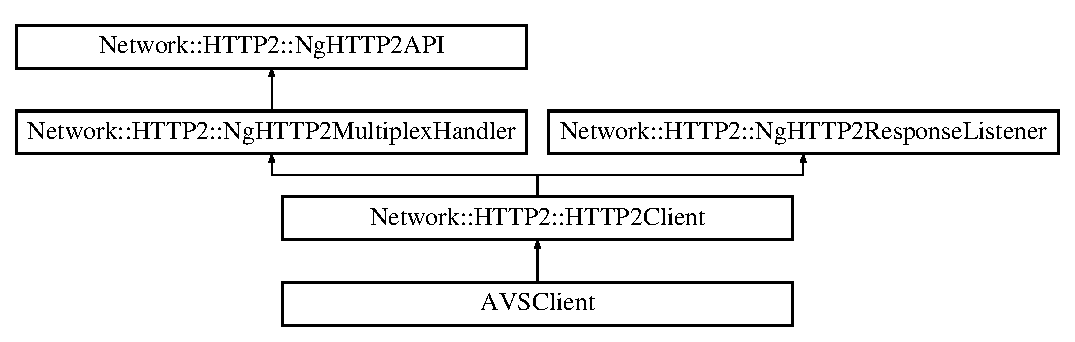
\includegraphics[height=4.000000cm]{de/d9b/classNetwork_1_1HTTP2_1_1HTTP2Client}
\end{center}
\end{figure}
\subsection*{Public Member Functions}
\begin{DoxyCompactItemize}
\item 
\mbox{\Hypertarget{classNetwork_1_1HTTP2_1_1HTTP2Client_a29102db8089b67719318850c187a9461}\label{classNetwork_1_1HTTP2_1_1HTTP2Client_a29102db8089b67719318850c187a9461}} 
{\bfseries H\+T\+T\+P2\+Client} (const string url)
\item 
\mbox{\Hypertarget{classNetwork_1_1HTTP2_1_1HTTP2Client_af1623f17ea95731422d9f1d3b30bacc3}\label{classNetwork_1_1HTTP2_1_1HTTP2Client_af1623f17ea95731422d9f1d3b30bacc3}} 
void {\bfseries init\+Connection} (nghttp2\+\_\+nv $\ast$header\+\_\+data, size\+\_\+t header\+\_\+len, int $\ast$stream\+\_\+status)
\item 
\mbox{\Hypertarget{classNetwork_1_1HTTP2_1_1HTTP2Client_a9c27847775264d7a22a3bfb521c6cb9e}\label{classNetwork_1_1HTTP2_1_1HTTP2Client_a9c27847775264d7a22a3bfb521c6cb9e}} 
void {\bfseries push\+Stream\+Request} (Stream\+Queue\+Event event)
\item 
\mbox{\Hypertarget{classNetwork_1_1HTTP2_1_1HTTP2Client_a3c7c129cb3df6bd54c08ece2cfa47a9e}\label{classNetwork_1_1HTTP2_1_1HTTP2Client_a3c7c129cb3df6bd54c08ece2cfa47a9e}} 
\hyperlink{classNetwork_1_1HTTP2_1_1HTTP2ClientEventManager}{H\+T\+T\+P2\+Client\+Event\+Manager} $\ast$ {\bfseries get\+Event\+Manager} (void)
\item 
\mbox{\Hypertarget{classNetwork_1_1HTTP2_1_1HTTP2Client_afa6dd0f850970813f0d4727ce89a68cc}\label{classNetwork_1_1HTTP2_1_1HTTP2Client_afa6dd0f850970813f0d4727ce89a68cc}} 
\hyperlink{classNetwork_1_1HTTP_1_1HTTPResponse}{H\+T\+T\+P\+Response} $\ast$ {\bfseries get\+Response} (void)
\item 
\mbox{\Hypertarget{classNetwork_1_1HTTP2_1_1HTTP2Client_a13d1a42037119b5cb0dfb34c47beb9ef}\label{classNetwork_1_1HTTP2_1_1HTTP2Client_a13d1a42037119b5cb0dfb34c47beb9ef}} 
void {\bfseries on\+Response\+Event} (\hyperlink{structNetwork_1_1HTTP2_1_1HTTP2HandlerResponse}{H\+T\+T\+P2\+Handler\+Response} $\ast$response)
\item 
\mbox{\Hypertarget{classNetwork_1_1HTTP2_1_1HTTP2Client_af3f0eae097815ff7c1c706dae9934382}\label{classNetwork_1_1HTTP2_1_1HTTP2Client_af3f0eae097815ff7c1c706dae9934382}} 
void {\bfseries on\+Response\+Header\+Status\+Event} (const char $\ast$status\+\_\+code)
\item 
void \hyperlink{classNetwork_1_1HTTP2_1_1HTTP2Client_a5c5cd10569102998104f2124a3c7a119}{stream\+\_\+loop} (struct event\+\_\+base $\ast$evbase)
\begin{DoxyCompactList}\small\item\em stream\+\_\+loop \end{DoxyCompactList}\item 
\mbox{\Hypertarget{classNetwork_1_1HTTP2_1_1HTTP2Client_a8b134b7cf7b96b2b1c7f6f65636b630e}\label{classNetwork_1_1HTTP2_1_1HTTP2Client_a8b134b7cf7b96b2b1c7f6f65636b630e}} 
virtual \hyperlink{structNetwork_1_1HTTP2_1_1StreamQueueData}{Stream\+Queue\+Data} $\ast$ {\bfseries on\+Process\+Stream\+Event} (Stream\+Queue\+Event event)=0
\item 
\mbox{\Hypertarget{classNetwork_1_1HTTP2_1_1HTTP2Client_aeecc6cec389077e163cee57bb1e626b0}\label{classNetwork_1_1HTTP2_1_1HTTP2Client_aeecc6cec389077e163cee57bb1e626b0}} 
virtual void {\bfseries on\+Stream\+Loop\+Start\+Event} (void)=0
\item 
\mbox{\Hypertarget{classNetwork_1_1HTTP2_1_1HTTP2Client_a286cbb2cb6406ddd6514aeee757f2aae}\label{classNetwork_1_1HTTP2_1_1HTTP2Client_a286cbb2cb6406ddd6514aeee757f2aae}} 
virtual void {\bfseries on\+Stream\+Loop\+Wait\+Event} (void)=0
\end{DoxyCompactItemize}
\subsection*{Protected Attributes}
\begin{DoxyCompactItemize}
\item 
\mbox{\Hypertarget{classNetwork_1_1HTTP2_1_1HTTP2Client_a0038606058e6f5dd9f77adfced2a7ffe}\label{classNetwork_1_1HTTP2_1_1HTTP2Client_a0038606058e6f5dd9f77adfced2a7ffe}} 
std\+::string {\bfseries m\+\_\+base\+\_\+url}
\item 
\mbox{\Hypertarget{classNetwork_1_1HTTP2_1_1HTTP2Client_afad154fd7ed41e5c7f0f8829952ff44f}\label{classNetwork_1_1HTTP2_1_1HTTP2Client_afad154fd7ed41e5c7f0f8829952ff44f}} 
\hyperlink{structNetwork_1_1HTTP2_1_1HTTP2HandlerResponse}{H\+T\+T\+P2\+Handler\+Response} $\ast$ {\bfseries m\+\_\+http2\+\_\+handler\+\_\+response}
\item 
\mbox{\Hypertarget{classNetwork_1_1HTTP2_1_1HTTP2Client_a83fe546902bc6be3fd2006c9517cb218}\label{classNetwork_1_1HTTP2_1_1HTTP2Client_a83fe546902bc6be3fd2006c9517cb218}} 
\hyperlink{classNetwork_1_1HTTP2_1_1NgHTTP2ResponseManager}{Ng\+H\+T\+T\+P2\+Response\+Manager} $\ast$ {\bfseries m\+\_\+http2\+\_\+response\+\_\+manager}
\item 
\mbox{\Hypertarget{classNetwork_1_1HTTP2_1_1HTTP2Client_a54262bf3e08d6ad8a6eca39fe8d6b02f}\label{classNetwork_1_1HTTP2_1_1HTTP2Client_a54262bf3e08d6ad8a6eca39fe8d6b02f}} 
\hyperlink{classNetwork_1_1HTTP2_1_1HTTP2ClientEventManager}{H\+T\+T\+P2\+Client\+Event\+Manager} $\ast$ {\bfseries m\+\_\+http2\+\_\+event\+\_\+manager}
\item 
\mbox{\Hypertarget{classNetwork_1_1HTTP2_1_1HTTP2Client_a82bad5a94c9004a1e586a53bd99c8b3b}\label{classNetwork_1_1HTTP2_1_1HTTP2Client_a82bad5a94c9004a1e586a53bd99c8b3b}} 
\hyperlink{classNetwork_1_1HTTP_1_1HTTPResponse}{H\+T\+T\+P\+Response} $\ast$ {\bfseries m\+\_\+http\+\_\+output\+\_\+response}
\end{DoxyCompactItemize}
\subsection*{Additional Inherited Members}


\subsection{Member Function Documentation}
\mbox{\Hypertarget{classNetwork_1_1HTTP2_1_1HTTP2Client_a5c5cd10569102998104f2124a3c7a119}\label{classNetwork_1_1HTTP2_1_1HTTP2Client_a5c5cd10569102998104f2124a3c7a119}} 
\index{Network\+::\+H\+T\+T\+P2\+::\+H\+T\+T\+P2\+Client@{Network\+::\+H\+T\+T\+P2\+::\+H\+T\+T\+P2\+Client}!stream\+\_\+loop@{stream\+\_\+loop}}
\index{stream\+\_\+loop@{stream\+\_\+loop}!Network\+::\+H\+T\+T\+P2\+::\+H\+T\+T\+P2\+Client@{Network\+::\+H\+T\+T\+P2\+::\+H\+T\+T\+P2\+Client}}
\subsubsection{\texorpdfstring{stream\+\_\+loop()}{stream\_loop()}}
{\footnotesize\ttfamily void H\+T\+T\+P2\+Client\+::stream\+\_\+loop (\begin{DoxyParamCaption}\item[{struct event\+\_\+base $\ast$}]{evbase }\end{DoxyParamCaption})\hspace{0.3cm}{\ttfamily [virtual]}}



stream\+\_\+loop 

override it ... 
\begin{DoxyParams}{Parameters}
{\em handler} & \\
\hline
\end{DoxyParams}


Implements \hyperlink{classNetwork_1_1HTTP2_1_1NgHTTP2MultiplexHandler_a95e9df9737af24d79894320e8cb343de}{Network\+::\+H\+T\+T\+P2\+::\+Ng\+H\+T\+T\+P2\+Multiplex\+Handler}.



The documentation for this class was generated from the following files\+:\begin{DoxyCompactItemize}
\item 
/home/mutzi/progs/linux\+\_\+workspace/alexa-\/avs-\/prototype/src/include/http2client.\+h\item 
/home/mutzi/progs/linux\+\_\+workspace/alexa-\/avs-\/prototype/src/http2client.\+cpp\end{DoxyCompactItemize}

\hypertarget{classNetwork_1_1HTTP2_1_1HTTP2ClientEventManager}{}\section{Network\+:\+:H\+T\+T\+P2\+:\+:H\+T\+T\+P2\+Client\+Event\+Manager Class Reference}
\label{classNetwork_1_1HTTP2_1_1HTTP2ClientEventManager}\index{Network\+::\+H\+T\+T\+P2\+::\+H\+T\+T\+P2\+Client\+Event\+Manager@{Network\+::\+H\+T\+T\+P2\+::\+H\+T\+T\+P2\+Client\+Event\+Manager}}
\subsection*{Public Member Functions}
\begin{DoxyCompactItemize}
\item 
\mbox{\Hypertarget{classNetwork_1_1HTTP2_1_1HTTP2ClientEventManager_a2fa38d058afbe4f01c86703df523e702}\label{classNetwork_1_1HTTP2_1_1HTTP2ClientEventManager_a2fa38d058afbe4f01c86703df523e702}} 
void {\bfseries register\+Directiven\+Listener} (\hyperlink{classNetwork_1_1HTTP_1_1DirectivenListener}{Directiven\+Listener} $\ast$listener)
\item 
\mbox{\Hypertarget{classNetwork_1_1HTTP2_1_1HTTP2ClientEventManager_a7c619296724ac41e95769239aa2cb50f}\label{classNetwork_1_1HTTP2_1_1HTTP2ClientEventManager_a7c619296724ac41e95769239aa2cb50f}} 
void {\bfseries unregister\+Directiven\+Listener} (\hyperlink{classNetwork_1_1HTTP_1_1DirectivenListener}{Directiven\+Listener} $\ast$listener)
\item 
\mbox{\Hypertarget{classNetwork_1_1HTTP2_1_1HTTP2ClientEventManager_afc79100de7cc9d8e4f5712b57b605f90}\label{classNetwork_1_1HTTP2_1_1HTTP2ClientEventManager_afc79100de7cc9d8e4f5712b57b605f90}} 
void {\bfseries register\+Audio\+Directiven\+Listener} (\hyperlink{classNetwork_1_1HTTP_1_1AudioPlayerDirectivenListener}{Audio\+Player\+Directiven\+Listener} $\ast$listener)
\item 
\mbox{\Hypertarget{classNetwork_1_1HTTP2_1_1HTTP2ClientEventManager_ab42d414c770b66f56b47abfcd5f5428c}\label{classNetwork_1_1HTTP2_1_1HTTP2ClientEventManager_ab42d414c770b66f56b47abfcd5f5428c}} 
void {\bfseries unregister\+Audio\+Directiven\+Listener} (\hyperlink{classNetwork_1_1HTTP_1_1AudioPlayerDirectivenListener}{Audio\+Player\+Directiven\+Listener} $\ast$listener)
\item 
\mbox{\Hypertarget{classNetwork_1_1HTTP2_1_1HTTP2ClientEventManager_ab0dcc078f1500f69903d9956ec50cf20}\label{classNetwork_1_1HTTP2_1_1HTTP2ClientEventManager_ab0dcc078f1500f69903d9956ec50cf20}} 
virtual void {\bfseries invoke\+All\+Events} (\hyperlink{classNetwork_1_1HTTP_1_1HTTPResponse}{H\+T\+T\+P\+Response} $\ast$response)
\item 
\mbox{\Hypertarget{classNetwork_1_1HTTP2_1_1HTTP2ClientEventManager_ab5bdbbcdd686b974a61e1ca0a045570f}\label{classNetwork_1_1HTTP2_1_1HTTP2ClientEventManager_ab5bdbbcdd686b974a61e1ca0a045570f}} 
void {\bfseries set\+Down\+Channel\+Status} (bool status)
\item 
\mbox{\Hypertarget{classNetwork_1_1HTTP2_1_1HTTP2ClientEventManager_ada68eb3ae12bb259540cad78ac455d1f}\label{classNetwork_1_1HTTP2_1_1HTTP2ClientEventManager_ada68eb3ae12bb259540cad78ac455d1f}} 
int $\ast$ {\bfseries get\+Stream\+Status} (void)
\item 
\mbox{\Hypertarget{classNetwork_1_1HTTP2_1_1HTTP2ClientEventManager_a30df0cab5c3fc8c0dbb090b51ef0afb8}\label{classNetwork_1_1HTTP2_1_1HTTP2ClientEventManager_a30df0cab5c3fc8c0dbb090b51ef0afb8}} 
void {\bfseries set\+Boundary} (std\+::string boundary)
\item 
bool \hyperlink{classNetwork_1_1HTTP2_1_1HTTP2ClientEventManager_ac7ae33977250bde85715967dc52ae1cf}{get\+Down\+Channel\+Status} (void)
\begin{DoxyCompactList}\small\item\em get\+Down\+Channel\+Status \end{DoxyCompactList}\end{DoxyCompactItemize}
\subsection*{Protected Member Functions}
\begin{DoxyCompactItemize}
\item 
\mbox{\Hypertarget{classNetwork_1_1HTTP2_1_1HTTP2ClientEventManager_ad9625a75a8e37ef43af1e22ac6d372bc}\label{classNetwork_1_1HTTP2_1_1HTTP2ClientEventManager_ad9625a75a8e37ef43af1e22ac6d372bc}} 
void {\bfseries invoke\+Recognize\+Event} (H\+T\+T\+P\+Client\+Recognize\+Directive $\ast$listener, \hyperlink{classNetwork_1_1HTTP_1_1HTTPClientDirectiveEvent}{H\+T\+T\+P\+Client\+Directive\+Event} $\ast$event)
\item 
\mbox{\Hypertarget{classNetwork_1_1HTTP2_1_1HTTP2ClientEventManager_a6becf5f240cc72e4df027badd4fa48bd}\label{classNetwork_1_1HTTP2_1_1HTTP2ClientEventManager_a6becf5f240cc72e4df027badd4fa48bd}} 
\hyperlink{classNetwork_1_1HTTP_1_1HTTPClientDirectiveEvent}{H\+T\+T\+P\+Client\+Directive\+Event} $\ast$ {\bfseries http\+\_\+response\+\_\+analyse} (\hyperlink{classNetwork_1_1HTTP_1_1HTTPResponse}{H\+T\+T\+P\+Response} $\ast$response)
\end{DoxyCompactItemize}
\subsection*{Protected Attributes}
\begin{DoxyCompactItemize}
\item 
\mbox{\Hypertarget{classNetwork_1_1HTTP2_1_1HTTP2ClientEventManager_a87be06424810bab439666bca577a1d95}\label{classNetwork_1_1HTTP2_1_1HTTP2ClientEventManager_a87be06424810bab439666bca577a1d95}} 
Directiven\+Listener\+List {\bfseries m\+\_\+directiven\+\_\+listener\+\_\+list}
\item 
\mbox{\Hypertarget{classNetwork_1_1HTTP2_1_1HTTP2ClientEventManager_ad8a290cb2755a2ab022eb44668f4a213}\label{classNetwork_1_1HTTP2_1_1HTTP2ClientEventManager_ad8a290cb2755a2ab022eb44668f4a213}} 
Audio\+Directiven\+List {\bfseries m\+\_\+audio\+\_\+directiven\+\_\+listener\+\_\+list}
\item 
\mbox{\Hypertarget{classNetwork_1_1HTTP2_1_1HTTP2ClientEventManager_a3c2106e0009d998c89f53e4ea2576927}\label{classNetwork_1_1HTTP2_1_1HTTP2ClientEventManager_a3c2106e0009d998c89f53e4ea2576927}} 
int $\ast$ {\bfseries m\+\_\+stream\+\_\+status}
\item 
\mbox{\Hypertarget{classNetwork_1_1HTTP2_1_1HTTP2ClientEventManager_af2b8875e7c125c0f0c1682aa6b733b32}\label{classNetwork_1_1HTTP2_1_1HTTP2ClientEventManager_af2b8875e7c125c0f0c1682aa6b733b32}} 
bool {\bfseries m\+\_\+downchannel\+\_\+status}
\item 
\mbox{\Hypertarget{classNetwork_1_1HTTP2_1_1HTTP2ClientEventManager_a9ede54148c4aa343e5cdfaef8f85991f}\label{classNetwork_1_1HTTP2_1_1HTTP2ClientEventManager_a9ede54148c4aa343e5cdfaef8f85991f}} 
std\+::string {\bfseries m\+\_\+boundary}
\end{DoxyCompactItemize}


\subsection{Member Function Documentation}
\mbox{\Hypertarget{classNetwork_1_1HTTP2_1_1HTTP2ClientEventManager_ac7ae33977250bde85715967dc52ae1cf}\label{classNetwork_1_1HTTP2_1_1HTTP2ClientEventManager_ac7ae33977250bde85715967dc52ae1cf}} 
\index{Network\+::\+H\+T\+T\+P2\+::\+H\+T\+T\+P2\+Client\+Event\+Manager@{Network\+::\+H\+T\+T\+P2\+::\+H\+T\+T\+P2\+Client\+Event\+Manager}!get\+Down\+Channel\+Status@{get\+Down\+Channel\+Status}}
\index{get\+Down\+Channel\+Status@{get\+Down\+Channel\+Status}!Network\+::\+H\+T\+T\+P2\+::\+H\+T\+T\+P2\+Client\+Event\+Manager@{Network\+::\+H\+T\+T\+P2\+::\+H\+T\+T\+P2\+Client\+Event\+Manager}}
\subsubsection{\texorpdfstring{get\+Down\+Channel\+Status()}{getDownChannelStatus()}}
{\footnotesize\ttfamily bool H\+T\+T\+P2\+Client\+Event\+Manager\+::get\+Down\+Channel\+Status (\begin{DoxyParamCaption}\item[{void}]{ }\end{DoxyParamCaption})}



get\+Down\+Channel\+Status 

\begin{DoxyReturn}{Returns}
if true downchannel is up if false downchannel is down 
\end{DoxyReturn}


The documentation for this class was generated from the following files\+:\begin{DoxyCompactItemize}
\item 
/home/mutzi/progs/linux\+\_\+workspace/alexa-\/avs-\/prototype/src/include/http2clienteventmanager.\+h\item 
/home/mutzi/progs/linux\+\_\+workspace/alexa-\/avs-\/prototype/src/http2clienteventmanager.\+cpp\end{DoxyCompactItemize}

\hypertarget{structNetwork_1_1HTTP2_1_1HTTP2HandlerResponse}{}\section{Network\+:\+:H\+T\+T\+P2\+:\+:H\+T\+T\+P2\+Handler\+Response Struct Reference}
\label{structNetwork_1_1HTTP2_1_1HTTP2HandlerResponse}\index{Network\+::\+H\+T\+T\+P2\+::\+H\+T\+T\+P2\+Handler\+Response@{Network\+::\+H\+T\+T\+P2\+::\+H\+T\+T\+P2\+Handler\+Response}}
\subsection*{Public Attributes}
\begin{DoxyCompactItemize}
\item 
\mbox{\Hypertarget{structNetwork_1_1HTTP2_1_1HTTP2HandlerResponse_a0ff9bf4cac8ddee31482c3b0ce788d85}\label{structNetwork_1_1HTTP2_1_1HTTP2HandlerResponse_a0ff9bf4cac8ddee31482c3b0ce788d85}} 
char $\ast$ {\bfseries memory}
\item 
\mbox{\Hypertarget{structNetwork_1_1HTTP2_1_1HTTP2HandlerResponse_a0a65650181e3502eec604fd7ec4f11f3}\label{structNetwork_1_1HTTP2_1_1HTTP2HandlerResponse_a0a65650181e3502eec604fd7ec4f11f3}} 
size\+\_\+t {\bfseries size}
\end{DoxyCompactItemize}


The documentation for this struct was generated from the following file\+:\begin{DoxyCompactItemize}
\item 
/home/mutzi/progs/linux\+\_\+workspace/alexa-\/avs-\/prototype/src/include/nghttp2handler.\+h\end{DoxyCompactItemize}

\hypertarget{structNetwork_1_1HTTP2_1_1HTTP2HandlerResponseManagement}{}\section{Network\+:\+:H\+T\+T\+P2\+:\+:H\+T\+T\+P2\+Handler\+Response\+Management Struct Reference}
\label{structNetwork_1_1HTTP2_1_1HTTP2HandlerResponseManagement}\index{Network\+::\+H\+T\+T\+P2\+::\+H\+T\+T\+P2\+Handler\+Response\+Management@{Network\+::\+H\+T\+T\+P2\+::\+H\+T\+T\+P2\+Handler\+Response\+Management}}
\subsection*{Public Attributes}
\begin{DoxyCompactItemize}
\item 
\mbox{\Hypertarget{structNetwork_1_1HTTP2_1_1HTTP2HandlerResponseManagement_a06e2de580e20b608db15f6d42a35666a}\label{structNetwork_1_1HTTP2_1_1HTTP2HandlerResponseManagement_a06e2de580e20b608db15f6d42a35666a}} 
\hyperlink{classNetwork_1_1HTTP2_1_1NgHTTP2ResponseManager}{Ng\+H\+T\+T\+P2\+Response\+Manager} $\ast$ {\bfseries manager}
\item 
\mbox{\Hypertarget{structNetwork_1_1HTTP2_1_1HTTP2HandlerResponseManagement_a198d98197519e981af7ef7cdc4811f1b}\label{structNetwork_1_1HTTP2_1_1HTTP2HandlerResponseManagement_a198d98197519e981af7ef7cdc4811f1b}} 
\hyperlink{structNetwork_1_1HTTP2_1_1HTTP2HandlerResponse}{H\+T\+T\+P2\+Handler\+Response} $\ast$ {\bfseries response\+\_\+memory}
\end{DoxyCompactItemize}


The documentation for this struct was generated from the following file\+:\begin{DoxyCompactItemize}
\item 
/home/mutzi/progs/linux\+\_\+workspace/alexa-\/avs-\/prototype/src/include/nghttp2handler.\+h\end{DoxyCompactItemize}

\hypertarget{structNetwork_1_1HTTP2_1_1HTTP2HandlerSession}{}\section{Network\+:\+:H\+T\+T\+P2\+:\+:H\+T\+T\+P2\+Handler\+Session Struct Reference}
\label{structNetwork_1_1HTTP2_1_1HTTP2HandlerSession}\index{Network\+::\+H\+T\+T\+P2\+::\+H\+T\+T\+P2\+Handler\+Session@{Network\+::\+H\+T\+T\+P2\+::\+H\+T\+T\+P2\+Handler\+Session}}
\subsection*{Public Attributes}
\begin{DoxyCompactItemize}
\item 
\mbox{\Hypertarget{structNetwork_1_1HTTP2_1_1HTTP2HandlerSession_a0a6fe64e74c8bd333711aa30adb962d3}\label{structNetwork_1_1HTTP2_1_1HTTP2HandlerSession_a0a6fe64e74c8bd333711aa30adb962d3}} 
struct event\+\_\+base $\ast$ {\bfseries evbase}
\item 
\mbox{\Hypertarget{structNetwork_1_1HTTP2_1_1HTTP2HandlerSession_ac67e4db1227721ac0026af3e9267bc2b}\label{structNetwork_1_1HTTP2_1_1HTTP2HandlerSession_ac67e4db1227721ac0026af3e9267bc2b}} 
S\+S\+L\+\_\+\+C\+TX $\ast$ {\bfseries ssl\+\_\+ctx}
\item 
\mbox{\Hypertarget{structNetwork_1_1HTTP2_1_1HTTP2HandlerSession_a72dfa7a89e3b0b7c6659527fa1fb20f4}\label{structNetwork_1_1HTTP2_1_1HTTP2HandlerSession_a72dfa7a89e3b0b7c6659527fa1fb20f4}} 
const char $\ast$ {\bfseries host}
\item 
\mbox{\Hypertarget{structNetwork_1_1HTTP2_1_1HTTP2HandlerSession_ad4b26b5c59e4f67612cfb9c129c361a2}\label{structNetwork_1_1HTTP2_1_1HTTP2HandlerSession_ad4b26b5c59e4f67612cfb9c129c361a2}} 
uint16\+\_\+t {\bfseries port}
\item 
\mbox{\Hypertarget{structNetwork_1_1HTTP2_1_1HTTP2HandlerSession_a660d8104cefc3d346dbe3ddfeac26a79}\label{structNetwork_1_1HTTP2_1_1HTTP2HandlerSession_a660d8104cefc3d346dbe3ddfeac26a79}} 
\hyperlink{structNetwork_1_1HTTP2_1_1http2__session__data}{http2\+\_\+session\+\_\+data} $\ast$ {\bfseries session\+\_\+data}
\end{DoxyCompactItemize}


The documentation for this struct was generated from the following file\+:\begin{DoxyCompactItemize}
\item 
/home/mutzi/progs/linux\+\_\+workspace/alexa-\/avs-\/prototype/src/include/nghttp2handler.\+h\end{DoxyCompactItemize}

\hypertarget{classNetwork_1_1HTTP_1_1HTTP2Header}{}\section{Network\+:\+:H\+T\+TP\+:\+:H\+T\+T\+P2\+Header Class Reference}
\label{classNetwork_1_1HTTP_1_1HTTP2Header}\index{Network\+::\+H\+T\+T\+P\+::\+H\+T\+T\+P2\+Header@{Network\+::\+H\+T\+T\+P\+::\+H\+T\+T\+P2\+Header}}


H\+T\+T\+P/2 Message Headers.  




{\ttfamily \#include $<$http2header.\+h$>$}

\subsection*{Public Member Functions}
\begin{DoxyCompactItemize}
\item 
\mbox{\Hypertarget{classNetwork_1_1HTTP_1_1HTTP2Header_ac4ae5574f403cbdb1ae28a5282a5abef}\label{classNetwork_1_1HTTP_1_1HTTP2Header_ac4ae5574f403cbdb1ae28a5282a5abef}} 
{\bfseries H\+T\+T\+P2\+Header} (const std\+::string access\+\_\+token, const std\+::string event\+\_\+path)
\item 
\mbox{\Hypertarget{classNetwork_1_1HTTP_1_1HTTP2Header_a006f5aa2b6ff4c9b20a31a0fb952bcac}\label{classNetwork_1_1HTTP_1_1HTTP2Header_a006f5aa2b6ff4c9b20a31a0fb952bcac}} 
void {\bfseries set\+Methode} (const std\+::string methode)
\item 
\mbox{\Hypertarget{classNetwork_1_1HTTP_1_1HTTP2Header_acc8d27de57212e61b37f7b452520f234}\label{classNetwork_1_1HTTP_1_1HTTP2Header_acc8d27de57212e61b37f7b452520f234}} 
void {\bfseries set\+Sheme} (const std\+::string scheme)
\item 
\mbox{\Hypertarget{classNetwork_1_1HTTP_1_1HTTP2Header_a7da3c09b66e3931d6d5f765ebf2b3a9c}\label{classNetwork_1_1HTTP_1_1HTTP2Header_a7da3c09b66e3931d6d5f765ebf2b3a9c}} 
void {\bfseries set\+Path} (const std\+::string path)
\item 
\mbox{\Hypertarget{classNetwork_1_1HTTP_1_1HTTP2Header_a8dc45f9e96c072939d8cecf647db1341}\label{classNetwork_1_1HTTP_1_1HTTP2Header_a8dc45f9e96c072939d8cecf647db1341}} 
void {\bfseries set\+Authorization} (const std\+::string access\+\_\+token)
\item 
\mbox{\Hypertarget{classNetwork_1_1HTTP_1_1HTTP2Header_afccfca69595527cdafe5a7fbcd1888f4}\label{classNetwork_1_1HTTP_1_1HTTP2Header_afccfca69595527cdafe5a7fbcd1888f4}} 
void {\bfseries set\+Content\+Type} (const std\+::string content\+\_\+type)
\item 
\mbox{\Hypertarget{classNetwork_1_1HTTP_1_1HTTP2Header_a80aa6e5ca52a7e31f3689aa03f478e82}\label{classNetwork_1_1HTTP_1_1HTTP2Header_a80aa6e5ca52a7e31f3689aa03f478e82}} 
void {\bfseries set\+Boundary} (const std\+::string boundary)
\item 
\mbox{\Hypertarget{classNetwork_1_1HTTP_1_1HTTP2Header_ac958f22ab7db1c81b01913f964fc1022}\label{classNetwork_1_1HTTP_1_1HTTP2Header_ac958f22ab7db1c81b01913f964fc1022}} 
const std\+::string \& {\bfseries get\+Methode} (void) const
\item 
\mbox{\Hypertarget{classNetwork_1_1HTTP_1_1HTTP2Header_a93e4ae0fc20208acf725909bed9ea117}\label{classNetwork_1_1HTTP_1_1HTTP2Header_a93e4ae0fc20208acf725909bed9ea117}} 
const std\+::string \& {\bfseries get\+Sheme} (void) const
\item 
\mbox{\Hypertarget{classNetwork_1_1HTTP_1_1HTTP2Header_aecc9ae184d85fdadf5178e6f6d9e5f22}\label{classNetwork_1_1HTTP_1_1HTTP2Header_aecc9ae184d85fdadf5178e6f6d9e5f22}} 
const std\+::string \& {\bfseries get\+Path} (void) const
\item 
\mbox{\Hypertarget{classNetwork_1_1HTTP_1_1HTTP2Header_a7ef55dc3fb74bd91f46d7e6c32b59e44}\label{classNetwork_1_1HTTP_1_1HTTP2Header_a7ef55dc3fb74bd91f46d7e6c32b59e44}} 
const std\+::string \& {\bfseries get\+Access\+Token} (void) const
\item 
\mbox{\Hypertarget{classNetwork_1_1HTTP_1_1HTTP2Header_ad7c90dbb1c8cee061007f144621282d8}\label{classNetwork_1_1HTTP_1_1HTTP2Header_ad7c90dbb1c8cee061007f144621282d8}} 
const std\+::string \& {\bfseries get\+Content\+Type} (void) const
\item 
\mbox{\Hypertarget{classNetwork_1_1HTTP_1_1HTTP2Header_acc229166a69a7a26d272ec387309edf7}\label{classNetwork_1_1HTTP_1_1HTTP2Header_acc229166a69a7a26d272ec387309edf7}} 
const std\+::string \& {\bfseries get\+Boundary} (void) const
\end{DoxyCompactItemize}
\subsection*{Static Public Attributes}
\begin{DoxyCompactItemize}
\item 
\mbox{\Hypertarget{classNetwork_1_1HTTP_1_1HTTP2Header_ab9032cab42b1a181f2fe3c36e27898af}\label{classNetwork_1_1HTTP_1_1HTTP2Header_ab9032cab42b1a181f2fe3c36e27898af}} 
static std\+::string {\bfseries H\+T\+T\+P2\+\_\+\+H\+E\+A\+D\+E\+R\+M\+S\+G\+\_\+\+M\+E\+T\+H\+OD} = \char`\"{}\+:method =\char`\"{}
\item 
\mbox{\Hypertarget{classNetwork_1_1HTTP_1_1HTTP2Header_a985dd761e9bf960ff543669d56b024a8}\label{classNetwork_1_1HTTP_1_1HTTP2Header_a985dd761e9bf960ff543669d56b024a8}} 
static std\+::string {\bfseries H\+T\+T\+P2\+\_\+\+H\+E\+A\+D\+E\+R\+M\+S\+G\+\_\+\+S\+H\+E\+ME} = \char`\"{}\+:scheme =\char`\"{}
\item 
\mbox{\Hypertarget{classNetwork_1_1HTTP_1_1HTTP2Header_ab086b8e43fc776f32c98cc4eb5a570a6}\label{classNetwork_1_1HTTP_1_1HTTP2Header_ab086b8e43fc776f32c98cc4eb5a570a6}} 
static std\+::string {\bfseries H\+T\+T\+P2\+\_\+\+H\+E\+A\+D\+E\+R\+M\+S\+G\+\_\+\+P\+A\+TH} = \char`\"{}\+:path =\char`\"{}
\item 
\mbox{\Hypertarget{classNetwork_1_1HTTP_1_1HTTP2Header_a42fc3732482636cf906fdd766ce08c4f}\label{classNetwork_1_1HTTP_1_1HTTP2Header_a42fc3732482636cf906fdd766ce08c4f}} 
static std\+::string {\bfseries H\+T\+T\+P2\+\_\+\+H\+E\+A\+D\+E\+R\+M\+S\+G\+\_\+\+A\+U\+T\+H\+O\+R\+I\+Z\+A\+T\+I\+ON} = \char`\"{}authorization = Bearer \char`\"{}
\item 
\mbox{\Hypertarget{classNetwork_1_1HTTP_1_1HTTP2Header_aa38e7c6b7e97a0fb8b03029a1f33d765}\label{classNetwork_1_1HTTP_1_1HTTP2Header_aa38e7c6b7e97a0fb8b03029a1f33d765}} 
static std\+::string {\bfseries H\+T\+T\+P2\+\_\+\+H\+E\+A\+D\+E\+R\+M\+S\+G\+\_\+\+C\+O\+N\+T\+E\+N\+T\+\_\+\+T\+Y\+PE} = \char`\"{}content-\/type =\char`\"{}
\item 
\mbox{\Hypertarget{classNetwork_1_1HTTP_1_1HTTP2Header_a0cb32888b64de0e444b427fe526a00f0}\label{classNetwork_1_1HTTP_1_1HTTP2Header_a0cb32888b64de0e444b427fe526a00f0}} 
static std\+::string {\bfseries H\+T\+T\+P2\+\_\+\+H\+E\+A\+D\+E\+R\+M\+S\+G\+\_\+\+B\+O\+U\+N\+D\+A\+RY} = \char`\"{}boundary=\char`\"{}
\item 
\mbox{\Hypertarget{classNetwork_1_1HTTP_1_1HTTP2Header_a10fa685cb3887279330d5bbb2adb3a3a}\label{classNetwork_1_1HTTP_1_1HTTP2Header_a10fa685cb3887279330d5bbb2adb3a3a}} 
static std\+::string {\bfseries H\+T\+T\+P2\+\_\+\+P\+I\+NG} = \char`\"{}/ping\char`\"{}
\item 
\mbox{\Hypertarget{classNetwork_1_1HTTP_1_1HTTP2Header_a3c8bbf85c2e90b27d281928c24aba2fe}\label{classNetwork_1_1HTTP_1_1HTTP2Header_a3c8bbf85c2e90b27d281928c24aba2fe}} 
static std\+::string {\bfseries H\+T\+T\+P2\+\_\+\+E\+V\+E\+N\+T\+S\+\_\+\+E\+N\+D\+P\+O\+I\+NT} = \char`\"{}/v20160207/events\char`\"{}
\item 
\mbox{\Hypertarget{classNetwork_1_1HTTP_1_1HTTP2Header_ad0374b2131663d3fa3c3329d62af0e93}\label{classNetwork_1_1HTTP_1_1HTTP2Header_ad0374b2131663d3fa3c3329d62af0e93}} 
static std\+::string {\bfseries H\+T\+T\+P2\+\_\+\+D\+I\+R\+E\+C\+T\+I\+V\+E\+\_\+\+E\+N\+D\+P\+O\+I\+NT} = \char`\"{}/v20160207/directives\char`\"{}
\end{DoxyCompactItemize}


\subsection{Detailed Description}
H\+T\+T\+P/2 Message Headers. 

\+:method = \{\{verb\}\} \+:scheme = https \+:path = /\{\{A\+PI version\}\}/\{\{events or directives\}\} authorization = Bearer \{\{access\+\_\+token\}\} content-\/type = multipart/form-\/data; boundary=\{\{boundary\+\_\+term\}\} 

The documentation for this class was generated from the following files\+:\begin{DoxyCompactItemize}
\item 
/home/mutzi/progs/linux\+\_\+workspace/alexa-\/avs-\/prototype/src/include/http2header.\+h\item 
/home/mutzi/progs/linux\+\_\+workspace/alexa-\/avs-\/prototype/src/http2header.\+cpp\end{DoxyCompactItemize}

\hypertarget{classNetwork_1_1HTTP2_1_1HTTP2MultipartAnalyse}{}\section{Network\+:\+:H\+T\+T\+P2\+:\+:H\+T\+T\+P2\+Multipart\+Analyse Class Reference}
\label{classNetwork_1_1HTTP2_1_1HTTP2MultipartAnalyse}\index{Network\+::\+H\+T\+T\+P2\+::\+H\+T\+T\+P2\+Multipart\+Analyse@{Network\+::\+H\+T\+T\+P2\+::\+H\+T\+T\+P2\+Multipart\+Analyse}}
\subsection*{Public Member Functions}
\begin{DoxyCompactItemize}
\item 
\mbox{\Hypertarget{classNetwork_1_1HTTP2_1_1HTTP2MultipartAnalyse_a8095baf78ba7751fa825ed3c7af7cdab}\label{classNetwork_1_1HTTP2_1_1HTTP2MultipartAnalyse_a8095baf78ba7751fa825ed3c7af7cdab}} 
void {\bfseries analyse} (char $\ast$content, size\+\_\+t content\+\_\+size)
\item 
\mbox{\Hypertarget{classNetwork_1_1HTTP2_1_1HTTP2MultipartAnalyse_a726ea0b002f20515e3088e9f75b5b97a}\label{classNetwork_1_1HTTP2_1_1HTTP2MultipartAnalyse_a726ea0b002f20515e3088e9f75b5b97a}} 
void {\bfseries update} (\hyperlink{classNetwork_1_1HTTP_1_1HTTPClientDirectiveEvent}{H\+T\+T\+P\+Client\+Directive\+Event} $\ast$event)
\end{DoxyCompactItemize}
\subsection*{Protected Member Functions}
\begin{DoxyCompactItemize}
\item 
\mbox{\Hypertarget{classNetwork_1_1HTTP2_1_1HTTP2MultipartAnalyse_a68e226bc76e8107d253cf4c5c7e8629a}\label{classNetwork_1_1HTTP2_1_1HTTP2MultipartAnalyse_a68e226bc76e8107d253cf4c5c7e8629a}} 
size\+\_\+t {\bfseries next\+Entry\+Point} (char $\ast$content, size\+\_\+t offset, char delim)
\item 
\mbox{\Hypertarget{classNetwork_1_1HTTP2_1_1HTTP2MultipartAnalyse_a6f3139365b1a13706db5394392d1a3e4}\label{classNetwork_1_1HTTP2_1_1HTTP2MultipartAnalyse_a6f3139365b1a13706db5394392d1a3e4}} 
std\+::vector$<$ size\+\_\+t $>$ {\bfseries get\+Entry\+Positions} (char $\ast$content, size\+\_\+t size, unsigned int amount, std\+::string needle, unsigned int $\ast$real\+\_\+amount)
\item 
\mbox{\Hypertarget{classNetwork_1_1HTTP2_1_1HTTP2MultipartAnalyse_aa8869c2b1e4cf58188ce570f08c4543a}\label{classNetwork_1_1HTTP2_1_1HTTP2MultipartAnalyse_aa8869c2b1e4cf58188ce570f08c4543a}} 
size\+\_\+t {\bfseries search} (char $\ast$content, size\+\_\+t offset, size\+\_\+t size, std\+::string needle)
\item 
\mbox{\Hypertarget{classNetwork_1_1HTTP2_1_1HTTP2MultipartAnalyse_a855bf74fd45edae96ed2a17f6a7dfaef}\label{classNetwork_1_1HTTP2_1_1HTTP2MultipartAnalyse_a855bf74fd45edae96ed2a17f6a7dfaef}} 
void {\bfseries debug\+\_\+write\+\_\+file} (const char $\ast$file, const char $\ast$content, size\+\_\+t content\+\_\+size)
\end{DoxyCompactItemize}


The documentation for this class was generated from the following files\+:\begin{DoxyCompactItemize}
\item 
/home/mutzi/progs/linux\+\_\+workspace/alexa-\/avs-\/prototype/src/include/http2multipartanalyse.\+h\item 
/home/mutzi/progs/linux\+\_\+workspace/alexa-\/avs-\/prototype/src/http2multipartanalyse.\+cpp\end{DoxyCompactItemize}

\hypertarget{classNetwork_1_1HTTP_1_1HTTPClientDirectiveEvent}{}\section{Network\+:\+:H\+T\+TP\+:\+:H\+T\+T\+P\+Client\+Directive\+Event Class Reference}
\label{classNetwork_1_1HTTP_1_1HTTPClientDirectiveEvent}\index{Network\+::\+H\+T\+T\+P\+::\+H\+T\+T\+P\+Client\+Directive\+Event@{Network\+::\+H\+T\+T\+P\+::\+H\+T\+T\+P\+Client\+Directive\+Event}}
\subsection*{Public Member Functions}
\begin{DoxyCompactItemize}
\item 
\mbox{\Hypertarget{classNetwork_1_1HTTP_1_1HTTPClientDirectiveEvent_acbc914fb3b9706b26ac3609fca49ab60}\label{classNetwork_1_1HTTP_1_1HTTPClientDirectiveEvent_acbc914fb3b9706b26ac3609fca49ab60}} 
void {\bfseries add\+Json\+Object} (char $\ast$data, size\+\_\+t size)
\item 
\mbox{\Hypertarget{classNetwork_1_1HTTP_1_1HTTPClientDirectiveEvent_a8f02fb695e3c9b2ebbf66d07d75e292c}\label{classNetwork_1_1HTTP_1_1HTTPClientDirectiveEvent_a8f02fb695e3c9b2ebbf66d07d75e292c}} 
void {\bfseries add\+Audio\+Object} (char $\ast$data, size\+\_\+t size)
\item 
\mbox{\Hypertarget{classNetwork_1_1HTTP_1_1HTTPClientDirectiveEvent_a4bf514613a24ced321780eefff18d864}\label{classNetwork_1_1HTTP_1_1HTTPClientDirectiveEvent_a4bf514613a24ced321780eefff18d864}} 
\hyperlink{structNetwork_1_1HTTP_1_1JsonObject}{Json\+Object} $\ast$ {\bfseries get\+Json\+Object} (unsigned int position) const
\item 
\mbox{\Hypertarget{classNetwork_1_1HTTP_1_1HTTPClientDirectiveEvent_a197a9dc3086a4a8a0df994cc7e32f880}\label{classNetwork_1_1HTTP_1_1HTTPClientDirectiveEvent_a197a9dc3086a4a8a0df994cc7e32f880}} 
\hyperlink{structNetwork_1_1HTTP_1_1AudioObject}{Audio\+Object} $\ast$ {\bfseries get\+Audio\+Object} (unsigned int position) const
\item 
\mbox{\Hypertarget{classNetwork_1_1HTTP_1_1HTTPClientDirectiveEvent_ae1290f307234c3b777d0f807ec20b2e9}\label{classNetwork_1_1HTTP_1_1HTTPClientDirectiveEvent_ae1290f307234c3b777d0f807ec20b2e9}} 
unsigned int {\bfseries get\+Json\+Object\+Count} (void)
\item 
\mbox{\Hypertarget{classNetwork_1_1HTTP_1_1HTTPClientDirectiveEvent_a16bd2171956e5e7562d9c33b5c702bfd}\label{classNetwork_1_1HTTP_1_1HTTPClientDirectiveEvent_a16bd2171956e5e7562d9c33b5c702bfd}} 
unsigned int {\bfseries get\+Audio\+Object\+Count} (void)
\end{DoxyCompactItemize}


The documentation for this class was generated from the following files\+:\begin{DoxyCompactItemize}
\item 
/home/mutzi/progs/linux\+\_\+workspace/alexa-\/avs-\/prototype/src/include/httpclientdirectiveevent.\+h\item 
/home/mutzi/progs/linux\+\_\+workspace/alexa-\/avs-\/prototype/src/httpclientdirectiveevent.\+cpp\end{DoxyCompactItemize}

\hypertarget{classNetwork_1_1HTTP_1_1HTTPContent}{}\section{Network\+:\+:H\+T\+TP\+:\+:H\+T\+T\+P\+Content Class Reference}
\label{classNetwork_1_1HTTP_1_1HTTPContent}\index{Network\+::\+H\+T\+T\+P\+::\+H\+T\+T\+P\+Content@{Network\+::\+H\+T\+T\+P\+::\+H\+T\+T\+P\+Content}}
\subsection*{Public Member Functions}
\begin{DoxyCompactItemize}
\item 
\mbox{\Hypertarget{classNetwork_1_1HTTP_1_1HTTPContent_abe506faf6f1dbe781606101434f0fe7f}\label{classNetwork_1_1HTTP_1_1HTTPContent_abe506faf6f1dbe781606101434f0fe7f}} 
{\bfseries H\+T\+T\+P\+Content} (std\+::string content, H\+T\+T\+P\+Content\+Type type)
\item 
\mbox{\Hypertarget{classNetwork_1_1HTTP_1_1HTTPContent_ab4cde0d1977561cb6eba454829f184c0}\label{classNetwork_1_1HTTP_1_1HTTPContent_ab4cde0d1977561cb6eba454829f184c0}} 
{\bfseries H\+T\+T\+P\+Content} (char $\ast$content, H\+T\+T\+P\+Content\+Type type)
\item 
\mbox{\Hypertarget{classNetwork_1_1HTTP_1_1HTTPContent_a84862338e35fc61282d818529b330966}\label{classNetwork_1_1HTTP_1_1HTTPContent_a84862338e35fc61282d818529b330966}} 
void {\bfseries set\+Content\+Type} (H\+T\+T\+P\+Content\+Type type)
\item 
\mbox{\Hypertarget{classNetwork_1_1HTTP_1_1HTTPContent_a1f9f0dfcbfd829edb897eb600db68f45}\label{classNetwork_1_1HTTP_1_1HTTPContent_a1f9f0dfcbfd829edb897eb600db68f45}} 
void {\bfseries set\+Content} (char $\ast$content)
\item 
\mbox{\Hypertarget{classNetwork_1_1HTTP_1_1HTTPContent_a0e1e4b55b8b5c69b9b1ca63d6459c90c}\label{classNetwork_1_1HTTP_1_1HTTPContent_a0e1e4b55b8b5c69b9b1ca63d6459c90c}} 
char $\ast$ {\bfseries get\+Content} (void) const
\item 
\mbox{\Hypertarget{classNetwork_1_1HTTP_1_1HTTPContent_ac107938b129049aacdc218aff1b61a42}\label{classNetwork_1_1HTTP_1_1HTTPContent_ac107938b129049aacdc218aff1b61a42}} 
H\+T\+T\+P\+Content\+Type {\bfseries get\+Content\+Type} (void) const
\end{DoxyCompactItemize}


The documentation for this class was generated from the following files\+:\begin{DoxyCompactItemize}
\item 
/home/mutzi/progs/linux\+\_\+workspace/alexa-\/avs-\/prototype/src/include/httpcontent.\+h\item 
/home/mutzi/progs/linux\+\_\+workspace/alexa-\/avs-\/prototype/src/httpcontent.\+cpp\end{DoxyCompactItemize}

\hypertarget{classNetwork_1_1HTTP_1_1HTTPContentFactory}{}\section{Network\+:\+:H\+T\+TP\+:\+:H\+T\+T\+P\+Content\+Factory Class Reference}
\label{classNetwork_1_1HTTP_1_1HTTPContentFactory}\index{Network\+::\+H\+T\+T\+P\+::\+H\+T\+T\+P\+Content\+Factory@{Network\+::\+H\+T\+T\+P\+::\+H\+T\+T\+P\+Content\+Factory}}
\subsection*{Public Member Functions}
\begin{DoxyCompactItemize}
\item 
\mbox{\Hypertarget{classNetwork_1_1HTTP_1_1HTTPContentFactory_a806650365553ff6ac7e2e29f3cd044fe}\label{classNetwork_1_1HTTP_1_1HTTPContentFactory_a806650365553ff6ac7e2e29f3cd044fe}} 
\hyperlink{classNetwork_1_1HTTP_1_1HTTPContent}{H\+T\+T\+P\+Content} {\bfseries create\+J\+S\+O\+N\+Content} (const std\+::string json\+\_\+obj)
\item 
\mbox{\Hypertarget{classNetwork_1_1HTTP_1_1HTTPContentFactory_ab81b39432fda0ac873a9adf0b4b562d3}\label{classNetwork_1_1HTTP_1_1HTTPContentFactory_ab81b39432fda0ac873a9adf0b4b562d3}} 
\hyperlink{classNetwork_1_1HTTP_1_1HTTPContent}{H\+T\+T\+P\+Content} {\bfseries create\+Audio\+Content} (const char $\ast$audio)
\end{DoxyCompactItemize}


The documentation for this class was generated from the following files\+:\begin{DoxyCompactItemize}
\item 
/home/mutzi/progs/linux\+\_\+workspace/alexa-\/avs-\/prototype/src/include/httpcontentfactory.\+h\item 
/home/mutzi/progs/linux\+\_\+workspace/alexa-\/avs-\/prototype/src/httpcontentfactory.\+cpp\end{DoxyCompactItemize}

\hypertarget{classNetwork_1_1HTTP_1_1HTTPCurlHandler}{}\section{Network\+:\+:H\+T\+TP\+:\+:H\+T\+T\+P\+Curl\+Handler Class Reference}
\label{classNetwork_1_1HTTP_1_1HTTPCurlHandler}\index{Network\+::\+H\+T\+T\+P\+::\+H\+T\+T\+P\+Curl\+Handler@{Network\+::\+H\+T\+T\+P\+::\+H\+T\+T\+P\+Curl\+Handler}}
Inheritance diagram for Network\+:\+:H\+T\+TP\+:\+:H\+T\+T\+P\+Curl\+Handler\+:\begin{figure}[H]
\begin{center}
\leavevmode
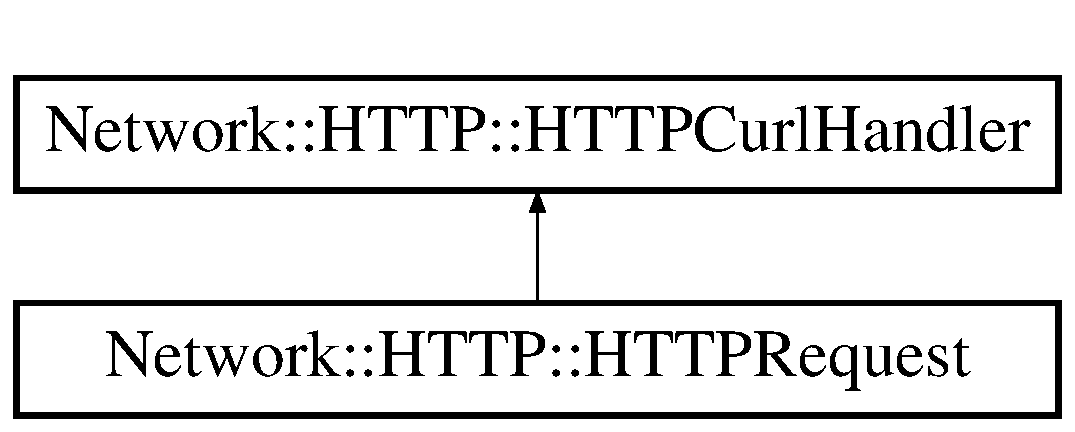
\includegraphics[height=2.000000cm]{dd/d92/classNetwork_1_1HTTP_1_1HTTPCurlHandler}
\end{center}
\end{figure}
\subsection*{Public Member Functions}
\begin{DoxyCompactItemize}
\item 
\mbox{\Hypertarget{classNetwork_1_1HTTP_1_1HTTPCurlHandler_a92de1090a6631a63369f956387d0627a}\label{classNetwork_1_1HTTP_1_1HTTPCurlHandler_a92de1090a6631a63369f956387d0627a}} 
virtual void {\bfseries init} ()
\item 
\mbox{\Hypertarget{classNetwork_1_1HTTP_1_1HTTPCurlHandler_a8a8acaf3560d2b0ecf5b2533a749e465}\label{classNetwork_1_1HTTP_1_1HTTPCurlHandler_a8a8acaf3560d2b0ecf5b2533a749e465}} 
void {\bfseries set\+Response\+Callback} (\hyperlink{structNetwork_1_1HTTP_1_1HTTPResponseMemory}{H\+T\+T\+P\+Response\+Memory} $\ast$chunk)  throw (std\+::exception )
\item 
\mbox{\Hypertarget{classNetwork_1_1HTTP_1_1HTTPCurlHandler_a09626294d8ba90d5d365200c44dda471}\label{classNetwork_1_1HTTP_1_1HTTPCurlHandler_a09626294d8ba90d5d365200c44dda471}} 
C\+U\+RL $\ast$ {\bfseries get\+Handle} (void)
\item 
\mbox{\Hypertarget{classNetwork_1_1HTTP_1_1HTTPCurlHandler_a4fcf7e210a14f48aca958e295a2055dd}\label{classNetwork_1_1HTTP_1_1HTTPCurlHandler_a4fcf7e210a14f48aca958e295a2055dd}} 
virtual void {\bfseries do\+It} (void)  throw ( std\+::exception )
\item 
\mbox{\Hypertarget{classNetwork_1_1HTTP_1_1HTTPCurlHandler_aa6ad1edac5930e5161d6154c8b812e3f}\label{classNetwork_1_1HTTP_1_1HTTPCurlHandler_aa6ad1edac5930e5161d6154c8b812e3f}} 
virtual void {\bfseries clean} ()
\end{DoxyCompactItemize}
\subsection*{Static Protected Member Functions}
\begin{DoxyCompactItemize}
\item 
\mbox{\Hypertarget{classNetwork_1_1HTTP_1_1HTTPCurlHandler_a1d4b5817614cf5e07e7da42cb9f6ab3e}\label{classNetwork_1_1HTTP_1_1HTTPCurlHandler_a1d4b5817614cf5e07e7da42cb9f6ab3e}} 
static size\+\_\+t {\bfseries Write\+Memory\+Callback} (void $\ast$contents, size\+\_\+t size, size\+\_\+t nmemb, void $\ast$userp)
\end{DoxyCompactItemize}
\subsection*{Protected Attributes}
\begin{DoxyCompactItemize}
\item 
\mbox{\Hypertarget{classNetwork_1_1HTTP_1_1HTTPCurlHandler_a87da1d90cd40c6ed90e97fd74698a6b4}\label{classNetwork_1_1HTTP_1_1HTTPCurlHandler_a87da1d90cd40c6ed90e97fd74698a6b4}} 
C\+U\+RL $\ast$ {\bfseries m\+\_\+curl\+\_\+handle}
\item 
\mbox{\Hypertarget{classNetwork_1_1HTTP_1_1HTTPCurlHandler_a338d584b47b509d09059ed64bb79b7af}\label{classNetwork_1_1HTTP_1_1HTTPCurlHandler_a338d584b47b509d09059ed64bb79b7af}} 
\hyperlink{structNetwork_1_1HTTP_1_1HTTPResponseMemory}{H\+T\+T\+P\+Response\+Memory} $\ast$ {\bfseries m\+\_\+response\+\_\+content}
\end{DoxyCompactItemize}


The documentation for this class was generated from the following files\+:\begin{DoxyCompactItemize}
\item 
/home/mutzi/progs/linux\+\_\+workspace/alexa-\/avs-\/prototype/src/include/httpcurlhandler.\+h\item 
/home/mutzi/progs/linux\+\_\+workspace/alexa-\/avs-\/prototype/src/httpcurlhandler.\+cpp\end{DoxyCompactItemize}

\hypertarget{classNetwork_1_1HTTP_1_1HTTPHeader}{}\section{Network\+:\+:H\+T\+TP\+:\+:H\+T\+T\+P\+Header Class Reference}
\label{classNetwork_1_1HTTP_1_1HTTPHeader}\index{Network\+::\+H\+T\+T\+P\+::\+H\+T\+T\+P\+Header@{Network\+::\+H\+T\+T\+P\+::\+H\+T\+T\+P\+Header}}


The \hyperlink{classNetwork_1_1HTTP_1_1HTTPHeader}{H\+T\+T\+P\+Header} class.  




{\ttfamily \#include $<$httpheader.\+h$>$}

\subsection*{Public Member Functions}
\begin{DoxyCompactItemize}
\item 
\mbox{\Hypertarget{classNetwork_1_1HTTP_1_1HTTPHeader_a56358fa12bd27707de8ad6cf947cd92d}\label{classNetwork_1_1HTTP_1_1HTTPHeader_a56358fa12bd27707de8ad6cf947cd92d}} 
{\bfseries H\+T\+T\+P\+Header} (const std\+::string boundary)
\item 
\mbox{\Hypertarget{classNetwork_1_1HTTP_1_1HTTPHeader_a6100fd84766656e8874479a75d494ba1}\label{classNetwork_1_1HTTP_1_1HTTPHeader_a6100fd84766656e8874479a75d494ba1}} 
{\bfseries H\+T\+T\+P\+Header} (const std\+::string content\+\_\+disposition, const std\+::string content\+\_\+tpye)
\item 
\mbox{\Hypertarget{classNetwork_1_1HTTP_1_1HTTPHeader_a1b488bbabdf4037e6dc58655f2f9dc91}\label{classNetwork_1_1HTTP_1_1HTTPHeader_a1b488bbabdf4037e6dc58655f2f9dc91}} 
void {\bfseries set\+Content\+Disposition} (const std\+::string content\+\_\+disposition)
\item 
\mbox{\Hypertarget{classNetwork_1_1HTTP_1_1HTTPHeader_a8d90949a97d4d019cbce3affabf2daf7}\label{classNetwork_1_1HTTP_1_1HTTPHeader_a8d90949a97d4d019cbce3affabf2daf7}} 
void {\bfseries set\+Content\+Type} (const std\+::string content\+\_\+type)
\item 
\mbox{\Hypertarget{classNetwork_1_1HTTP_1_1HTTPHeader_a056752befb5b801c1193b9e940d92e94}\label{classNetwork_1_1HTTP_1_1HTTPHeader_a056752befb5b801c1193b9e940d92e94}} 
void {\bfseries set\+Boundary} (const std\+::string boundary)
\item 
\mbox{\Hypertarget{classNetwork_1_1HTTP_1_1HTTPHeader_a0f05d5b3073374318284ea1b667dc183}\label{classNetwork_1_1HTTP_1_1HTTPHeader_a0f05d5b3073374318284ea1b667dc183}} 
const std\+::string \& {\bfseries get\+Content\+Disposition} (void) const
\item 
\mbox{\Hypertarget{classNetwork_1_1HTTP_1_1HTTPHeader_a2f4f982ef8eb3de60e75d3cee7cc21f1}\label{classNetwork_1_1HTTP_1_1HTTPHeader_a2f4f982ef8eb3de60e75d3cee7cc21f1}} 
const std\+::string \& {\bfseries get\+Content\+Type} (void) const
\item 
\mbox{\Hypertarget{classNetwork_1_1HTTP_1_1HTTPHeader_a869ed7b4658bcdb1aec32354a90e1f86}\label{classNetwork_1_1HTTP_1_1HTTPHeader_a869ed7b4658bcdb1aec32354a90e1f86}} 
const std\+::string \& {\bfseries get\+Boundary} (void) const
\end{DoxyCompactItemize}
\subsection*{Static Public Attributes}
\begin{DoxyCompactItemize}
\item 
\mbox{\Hypertarget{classNetwork_1_1HTTP_1_1HTTPHeader_a38ca07e5cbe32cfc51e22abad2fedae0}\label{classNetwork_1_1HTTP_1_1HTTPHeader_a38ca07e5cbe32cfc51e22abad2fedae0}} 
static std\+::string {\bfseries H\+T\+T\+P\+\_\+\+H\+E\+A\+D\+E\+R\+M\+S\+G\+\_\+\+C\+O\+N\+T\+E\+N\+T\+\_\+\+D\+I\+S\+P\+O\+S\+I\+T\+I\+ON} = \char`\"{}Content-\/Disposition\+: \char`\"{}
\item 
\mbox{\Hypertarget{classNetwork_1_1HTTP_1_1HTTPHeader_a22522701d469ddb20b5dd2d641f5e4f1}\label{classNetwork_1_1HTTP_1_1HTTPHeader_a22522701d469ddb20b5dd2d641f5e4f1}} 
static std\+::string {\bfseries H\+T\+T\+P\+\_\+\+H\+E\+A\+D\+E\+R\+M\+S\+G\+\_\+\+C\+O\+N\+T\+E\+N\+T\+\_\+\+T\+Y\+PE} = \char`\"{}Content-\/Type\+: \char`\"{}
\end{DoxyCompactItemize}


\subsection{Detailed Description}
The \hyperlink{classNetwork_1_1HTTP_1_1HTTPHeader}{H\+T\+T\+P\+Header} class. 

J\+S\+ON Header\+: Content-\/\+Disposition\+: form-\/data; name=\char`\"{}metadata\char`\"{} Content-\/\+Type\+: application/json; charset=U\+T\+F-\/8

Binary Audio Header\+: Content-\/\+Disposition\+: form-\/data; name=\char`\"{}audio\char`\"{} Content-\/\+Type\+: application/octet-\/stream 

The documentation for this class was generated from the following files\+:\begin{DoxyCompactItemize}
\item 
/home/mutzi/progs/linux\+\_\+workspace/alexa-\/avs-\/prototype/src/include/httpheader.\+h\item 
/home/mutzi/progs/linux\+\_\+workspace/alexa-\/avs-\/prototype/src/httpheader.\+cpp\end{DoxyCompactItemize}

\hypertarget{classNetwork_1_1HTTP_1_1HTTPHeaderFactory}{}\section{Network\+:\+:H\+T\+TP\+:\+:H\+T\+T\+P\+Header\+Factory Class Reference}
\label{classNetwork_1_1HTTP_1_1HTTPHeaderFactory}\index{Network\+::\+H\+T\+T\+P\+::\+H\+T\+T\+P\+Header\+Factory@{Network\+::\+H\+T\+T\+P\+::\+H\+T\+T\+P\+Header\+Factory}}


{\ttfamily \#include $<$httpheaderfactory.\+h$>$}

\subsection*{Public Member Functions}
\begin{DoxyCompactItemize}
\item 
\mbox{\Hypertarget{classNetwork_1_1HTTP_1_1HTTPHeaderFactory_a30385586c595933a3c52346c9e163c62}\label{classNetwork_1_1HTTP_1_1HTTPHeaderFactory_a30385586c595933a3c52346c9e163c62}} 
\hyperlink{classNetwork_1_1HTTP_1_1HTTP2Header}{H\+T\+T\+P2\+Header} {\bfseries create\+\_\+\+H\+T\+T\+P2\+\_\+\+P\+O\+ST} (const std\+::string access\+\_\+token, const std\+::string event\+\_\+or\+\_\+directive, const std\+::string boundary)
\item 
\mbox{\Hypertarget{classNetwork_1_1HTTP_1_1HTTPHeaderFactory_afd3427b234d82b0643bc08ccf5005154}\label{classNetwork_1_1HTTP_1_1HTTPHeaderFactory_afd3427b234d82b0643bc08ccf5005154}} 
\hyperlink{classNetwork_1_1HTTP_1_1HTTP2Header}{H\+T\+T\+P2\+Header} {\bfseries create\+\_\+\+H\+T\+T\+P2\+\_\+\+G\+ET} (const std\+::string access\+\_\+token, const std\+::string event\+\_\+or\+\_\+directive, const std\+::string boundary)
\item 
\mbox{\Hypertarget{classNetwork_1_1HTTP_1_1HTTPHeaderFactory_a821eedb7ff87430758fd564cbb583a97}\label{classNetwork_1_1HTTP_1_1HTTPHeaderFactory_a821eedb7ff87430758fd564cbb583a97}} 
\hyperlink{classNetwork_1_1HTTP_1_1HTTPHeader}{H\+T\+T\+P\+Header} {\bfseries create\+J\+S\+O\+N\+Header} (const std\+::string boundary)
\item 
\mbox{\Hypertarget{classNetwork_1_1HTTP_1_1HTTPHeaderFactory_a9954b144b199480ab53dfcb4c9a1c717}\label{classNetwork_1_1HTTP_1_1HTTPHeaderFactory_a9954b144b199480ab53dfcb4c9a1c717}} 
\hyperlink{classNetwork_1_1HTTP_1_1HTTPHeader}{H\+T\+T\+P\+Header} {\bfseries create\+Audio\+Header} (const std\+::string boundary)
\end{DoxyCompactItemize}
\subsection*{Static Public Attributes}
\begin{DoxyCompactItemize}
\item 
\mbox{\Hypertarget{classNetwork_1_1HTTP_1_1HTTPHeaderFactory_a9c2717b2b2a9e14f5bfaefe2f2942528}\label{classNetwork_1_1HTTP_1_1HTTPHeaderFactory_a9c2717b2b2a9e14f5bfaefe2f2942528}} 
static std\+::string {\bfseries E\+V\+E\+N\+T\+S\+\_\+\+E\+N\+D\+P\+O\+I\+NT} = \char`\"{}/v20160207/events\char`\"{}
\item 
\mbox{\Hypertarget{classNetwork_1_1HTTP_1_1HTTPHeaderFactory_afc245df4d2b4a8a9b3679d38eec1435f}\label{classNetwork_1_1HTTP_1_1HTTPHeaderFactory_afc245df4d2b4a8a9b3679d38eec1435f}} 
static std\+::string {\bfseries D\+I\+R\+E\+C\+T\+I\+V\+E\+S\+\_\+\+E\+N\+D\+P\+O\+I\+NT} = \char`\"{}/v20160207/directives\char`\"{}
\item 
\mbox{\Hypertarget{classNetwork_1_1HTTP_1_1HTTPHeaderFactory_ac2bd55cf0bd7880c321aa0bde414a7e1}\label{classNetwork_1_1HTTP_1_1HTTPHeaderFactory_ac2bd55cf0bd7880c321aa0bde414a7e1}} 
static std\+::string {\bfseries P\+I\+N\+G\+\_\+\+E\+N\+D\+P\+O\+I\+NT} = \char`\"{}/ping\char`\"{}
\end{DoxyCompactItemize}


\subsection{Detailed Description}
H\+T\+TP Request\+: Alexa Voice Service

Host\+: \href{https://avs-alexa-eu.amazon.com}{\tt https\+://avs-\/alexa-\/eu.\+amazon.\+com}

Request-\/\+Events\+: U\+RL\+: \href{https://avs-alexa-eu.amazon.com/v20160207/events}{\tt https\+://avs-\/alexa-\/eu.\+amazon.\+com/v20160207/events} Events\+\_\+\+Endpoint\+: /v20160207/events H\+T\+T\+P\+Method\+: P\+O\+ST Content\+: metadata audio

Directive\+: U\+RL\+: \href{https://avs-alexa-eu.amazon.com/v20160207/directives}{\tt https\+://avs-\/alexa-\/eu.\+amazon.\+com/v20160207/directives} Directives\+\_\+\+Endpoint\+: /v20160207/directives H\+T\+T\+P\+Method\+: G\+ET 

The documentation for this class was generated from the following files\+:\begin{DoxyCompactItemize}
\item 
/home/mutzi/progs/linux\+\_\+workspace/alexa-\/avs-\/prototype/src/include/httpheaderfactory.\+h\item 
/home/mutzi/progs/linux\+\_\+workspace/alexa-\/avs-\/prototype/src/httpheaderfactory.\+cpp\end{DoxyCompactItemize}

\hypertarget{classNetwork_1_1HTTP_1_1HTTPRequest}{}\section{Network\+:\+:H\+T\+TP\+:\+:H\+T\+T\+P\+Request Class Reference}
\label{classNetwork_1_1HTTP_1_1HTTPRequest}\index{Network\+::\+H\+T\+T\+P\+::\+H\+T\+T\+P\+Request@{Network\+::\+H\+T\+T\+P\+::\+H\+T\+T\+P\+Request}}
Inheritance diagram for Network\+:\+:H\+T\+TP\+:\+:H\+T\+T\+P\+Request\+:\begin{figure}[H]
\begin{center}
\leavevmode
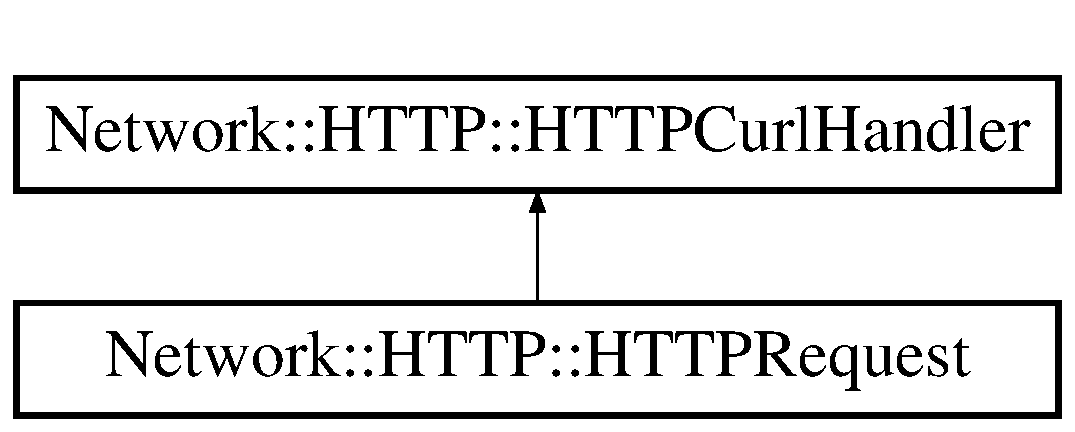
\includegraphics[height=2.000000cm]{d8/dd8/classNetwork_1_1HTTP_1_1HTTPRequest}
\end{center}
\end{figure}
\subsection*{Public Member Functions}
\begin{DoxyCompactItemize}
\item 
\mbox{\Hypertarget{classNetwork_1_1HTTP_1_1HTTPRequest_a171849a898d533a98d3f0c990da69f81}\label{classNetwork_1_1HTTP_1_1HTTPRequest_a171849a898d533a98d3f0c990da69f81}} 
{\bfseries H\+T\+T\+P\+Request} (const std\+::string \&url, \hyperlink{classNetwork_1_1HTTP_1_1HTTPResponse}{H\+T\+T\+P\+Response} $\ast$response)
\item 
\mbox{\Hypertarget{classNetwork_1_1HTTP_1_1HTTPRequest_a56baeab19cac0f566dc36fe3a2e54523}\label{classNetwork_1_1HTTP_1_1HTTPRequest_a56baeab19cac0f566dc36fe3a2e54523}} 
void {\bfseries add\+Header\+Data} (std\+::string header\+\_\+data)
\item 
\mbox{\Hypertarget{classNetwork_1_1HTTP_1_1HTTPRequest_a5bc18233f2aa7b6e2653f820469fb986}\label{classNetwork_1_1HTTP_1_1HTTPRequest_a5bc18233f2aa7b6e2653f820469fb986}} 
void {\bfseries write\+Header\+Data} ()
\item 
\mbox{\Hypertarget{classNetwork_1_1HTTP_1_1HTTPRequest_a6400e112a09b1f324d9ba118bbac7f6f}\label{classNetwork_1_1HTTP_1_1HTTPRequest_a6400e112a09b1f324d9ba118bbac7f6f}} 
void {\bfseries set\+Post\+Data} (std\+::string data)
\item 
\mbox{\Hypertarget{classNetwork_1_1HTTP_1_1HTTPRequest_a4a79ab13074db74c2b1e2f3991d4ac01}\label{classNetwork_1_1HTTP_1_1HTTPRequest_a4a79ab13074db74c2b1e2f3991d4ac01}} 
void {\bfseries clean} (void) final
\item 
\mbox{\Hypertarget{classNetwork_1_1HTTP_1_1HTTPRequest_a0aa1a681805c03a106d058ed9fdc7f20}\label{classNetwork_1_1HTTP_1_1HTTPRequest_a0aa1a681805c03a106d058ed9fdc7f20}} 
void {\bfseries do\+It} (void) final  throw (std\+::exception)
\end{DoxyCompactItemize}
\subsection*{Additional Inherited Members}


The documentation for this class was generated from the following files\+:\begin{DoxyCompactItemize}
\item 
/home/mutzi/progs/linux\+\_\+workspace/alexa-\/avs-\/prototype/src/include/httprequest.\+h\item 
/home/mutzi/progs/linux\+\_\+workspace/alexa-\/avs-\/prototype/src/httprequest.\+cpp\end{DoxyCompactItemize}

\hypertarget{structNetwork_1_1HTTP_1_1HTTPRequestMultipartContent}{}\section{Network\+:\+:H\+T\+TP\+:\+:H\+T\+T\+P\+Request\+Multipart\+Content Struct Reference}
\label{structNetwork_1_1HTTP_1_1HTTPRequestMultipartContent}\index{Network\+::\+H\+T\+T\+P\+::\+H\+T\+T\+P\+Request\+Multipart\+Content@{Network\+::\+H\+T\+T\+P\+::\+H\+T\+T\+P\+Request\+Multipart\+Content}}
\subsection*{Public Attributes}
\begin{DoxyCompactItemize}
\item 
\mbox{\Hypertarget{structNetwork_1_1HTTP_1_1HTTPRequestMultipartContent_adb6fbdfe9453fe958d52cdf2e1f6325c}\label{structNetwork_1_1HTTP_1_1HTTPRequestMultipartContent_adb6fbdfe9453fe958d52cdf2e1f6325c}} 
\hyperlink{classNetwork_1_1HTTP_1_1HTTPHeader}{H\+T\+T\+P\+Header} $\ast$ {\bfseries header\+\_\+one}
\item 
\mbox{\Hypertarget{structNetwork_1_1HTTP_1_1HTTPRequestMultipartContent_a1e8530fea42585b0eb8eb342ae0a8aa0}\label{structNetwork_1_1HTTP_1_1HTTPRequestMultipartContent_a1e8530fea42585b0eb8eb342ae0a8aa0}} 
\hyperlink{classNetwork_1_1HTTP_1_1HTTPHeader}{H\+T\+T\+P\+Header} $\ast$ {\bfseries header\+\_\+two}
\item 
\mbox{\Hypertarget{structNetwork_1_1HTTP_1_1HTTPRequestMultipartContent_af72994168bdf38244c1365a8ad6e8e9d}\label{structNetwork_1_1HTTP_1_1HTTPRequestMultipartContent_af72994168bdf38244c1365a8ad6e8e9d}} 
\hyperlink{classNetwork_1_1HTTP_1_1HTTPContent}{H\+T\+T\+P\+Content} $\ast$ {\bfseries content\+\_\+one}
\item 
\mbox{\Hypertarget{structNetwork_1_1HTTP_1_1HTTPRequestMultipartContent_a99e55c9a4e3f34832119be14674c93eb}\label{structNetwork_1_1HTTP_1_1HTTPRequestMultipartContent_a99e55c9a4e3f34832119be14674c93eb}} 
\hyperlink{classNetwork_1_1HTTP_1_1HTTPContent}{H\+T\+T\+P\+Content} $\ast$ {\bfseries content\+\_\+two}
\end{DoxyCompactItemize}


The documentation for this struct was generated from the following file\+:\begin{DoxyCompactItemize}
\item 
/home/mutzi/progs/linux\+\_\+workspace/alexa-\/avs-\/prototype/src/include/network.\+h\end{DoxyCompactItemize}

\hypertarget{classNetwork_1_1HTTP_1_1HTTPResponse}{}\section{Network\+:\+:H\+T\+TP\+:\+:H\+T\+T\+P\+Response Class Reference}
\label{classNetwork_1_1HTTP_1_1HTTPResponse}\index{Network\+::\+H\+T\+T\+P\+::\+H\+T\+T\+P\+Response@{Network\+::\+H\+T\+T\+P\+::\+H\+T\+T\+P\+Response}}
\subsection*{Public Member Functions}
\begin{DoxyCompactItemize}
\item 
\mbox{\Hypertarget{classNetwork_1_1HTTP_1_1HTTPResponse_a61b35ad0b64af2114b1fe41ccab3584c}\label{classNetwork_1_1HTTP_1_1HTTPResponse_a61b35ad0b64af2114b1fe41ccab3584c}} 
void {\bfseries set\+Content} (const char $\ast$content)
\item 
\mbox{\Hypertarget{classNetwork_1_1HTTP_1_1HTTPResponse_aa08f23a9aabb78996af2f409ee31a9a7}\label{classNetwork_1_1HTTP_1_1HTTPResponse_aa08f23a9aabb78996af2f409ee31a9a7}} 
void {\bfseries set\+Size} (size\+\_\+t size)
\item 
\mbox{\Hypertarget{classNetwork_1_1HTTP_1_1HTTPResponse_a8847fa066220168275002d7476a1be7c}\label{classNetwork_1_1HTTP_1_1HTTPResponse_a8847fa066220168275002d7476a1be7c}} 
const char $\ast$ {\bfseries get\+Content} (void) const
\item 
\mbox{\Hypertarget{classNetwork_1_1HTTP_1_1HTTPResponse_a062554f01c8b5aa22fc001cde532fd59}\label{classNetwork_1_1HTTP_1_1HTTPResponse_a062554f01c8b5aa22fc001cde532fd59}} 
size\+\_\+t {\bfseries get\+Size} (void) const
\end{DoxyCompactItemize}


The documentation for this class was generated from the following files\+:\begin{DoxyCompactItemize}
\item 
/home/mutzi/progs/linux\+\_\+workspace/alexa-\/avs-\/prototype/src/include/httpresponse.\+h\item 
/home/mutzi/progs/linux\+\_\+workspace/alexa-\/avs-\/prototype/src/httpresponse.\+cpp\end{DoxyCompactItemize}

\hypertarget{structNetwork_1_1HTTP_1_1HTTPResponseMemory}{}\section{Network\+:\+:H\+T\+TP\+:\+:H\+T\+T\+P\+Response\+Memory Struct Reference}
\label{structNetwork_1_1HTTP_1_1HTTPResponseMemory}\index{Network\+::\+H\+T\+T\+P\+::\+H\+T\+T\+P\+Response\+Memory@{Network\+::\+H\+T\+T\+P\+::\+H\+T\+T\+P\+Response\+Memory}}
\subsection*{Public Attributes}
\begin{DoxyCompactItemize}
\item 
\mbox{\Hypertarget{structNetwork_1_1HTTP_1_1HTTPResponseMemory_a251ce9ea73281ad889d5632ae24ee186}\label{structNetwork_1_1HTTP_1_1HTTPResponseMemory_a251ce9ea73281ad889d5632ae24ee186}} 
char $\ast$ {\bfseries memory}
\item 
\mbox{\Hypertarget{structNetwork_1_1HTTP_1_1HTTPResponseMemory_af3e7e51cb9581910665d7590fcee86b0}\label{structNetwork_1_1HTTP_1_1HTTPResponseMemory_af3e7e51cb9581910665d7590fcee86b0}} 
size\+\_\+t {\bfseries size}
\end{DoxyCompactItemize}


The documentation for this struct was generated from the following file\+:\begin{DoxyCompactItemize}
\item 
/home/mutzi/progs/linux\+\_\+workspace/alexa-\/avs-\/prototype/src/include/httpcurlhandler.\+h\end{DoxyCompactItemize}

\hypertarget{classnlohmann_1_1detail_1_1invalid__iterator}{}\section{nlohmann\+:\+:detail\+:\+:invalid\+\_\+iterator Class Reference}
\label{classnlohmann_1_1detail_1_1invalid__iterator}\index{nlohmann\+::detail\+::invalid\+\_\+iterator@{nlohmann\+::detail\+::invalid\+\_\+iterator}}


exception indicating errors with iterators  




{\ttfamily \#include $<$nlohmann\+\_\+json.\+h$>$}

Inheritance diagram for nlohmann\+:\+:detail\+:\+:invalid\+\_\+iterator\+:\begin{figure}[H]
\begin{center}
\leavevmode
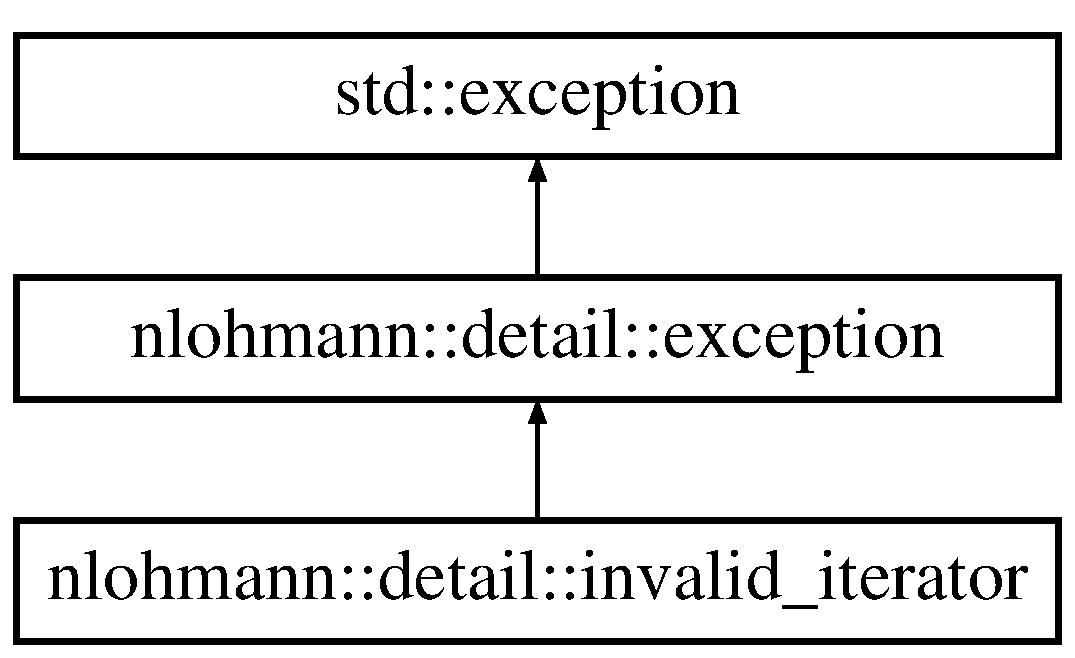
\includegraphics[height=3.000000cm]{d4/d5f/classnlohmann_1_1detail_1_1invalid__iterator}
\end{center}
\end{figure}
\subsection*{Static Public Member Functions}
\begin{DoxyCompactItemize}
\item 
\mbox{\Hypertarget{classnlohmann_1_1detail_1_1invalid__iterator_a48d724eccc74b550d695fc7575d9ce30}\label{classnlohmann_1_1detail_1_1invalid__iterator_a48d724eccc74b550d695fc7575d9ce30}} 
static \hyperlink{classnlohmann_1_1detail_1_1invalid__iterator}{invalid\+\_\+iterator} {\bfseries create} (int \hyperlink{classnlohmann_1_1detail_1_1exception_a0d4589a3fb54e81646d986c05efa3b9a}{id}, const \hyperlink{namespacenlohmann_1_1detail_a90aa5ef615aa8305e9ea20d8a947980fab45cffe084dd3d20d928bee85e7b0f21}{std\+::string} \&what\+\_\+arg)
\end{DoxyCompactItemize}
\subsection*{Additional Inherited Members}


\subsection{Detailed Description}
exception indicating errors with iterators 

Exceptions have ids 2xx.

\tabulinesep=1mm
\begin{longtabu} spread 0pt [c]{*{3}{|X[-1]}|}
\hline
\rowcolor{\tableheadbgcolor}\textbf{ name / id }&\textbf{ example massage }&\textbf{ description  }\\\cline{1-3}
\endfirsthead
\hline
\endfoot
\hline
\rowcolor{\tableheadbgcolor}\textbf{ name / id }&\textbf{ example massage }&\textbf{ description  }\\\cline{1-3}
\endhead
json.\+exception.\+invalid\+\_\+iterator.\+201 &iterators are not compatible &The iterators passed to constructor basic\+\_\+json(\+Input\+I\+T first, Input\+I\+T last) are not compatible, meaning they do not belong to the same container. Therefore, the range ({\itshape first}, {\itshape last}) is invalid. \\\cline{1-3}
json.\+exception.\+invalid\+\_\+iterator.\+202 &iterator does not fit current value &In an erase or insert function, the passed iterator {\itshape pos} does not belong to the J\+S\+ON value for which the function was called. It hence does not define a valid position for the deletion/insertion. \\\cline{1-3}
json.\+exception.\+invalid\+\_\+iterator.\+203 &iterators do not fit current value &Either iterator passed to function erase(\+Iterator\+Type first, Iterator\+Type last) does not belong to the J\+S\+ON value from which values shall be erased. It hence does not define a valid range to delete values from. \\\cline{1-3}
json.\+exception.\+invalid\+\_\+iterator.\+204 &iterators out of range &When an iterator range for a primitive type (number, boolean, or string) is passed to a constructor or an erase function, this range has to be exactly (begin(), end()), because this is the only way the single stored value is expressed. All other ranges are invalid. \\\cline{1-3}
json.\+exception.\+invalid\+\_\+iterator.\+205 &iterator out of range &When an iterator for a primitive type (number, boolean, or string) is passed to an erase function, the iterator has to be the begin() iterator, because it is the only way to address the stored value. All other iterators are invalid. \\\cline{1-3}
json.\+exception.\+invalid\+\_\+iterator.\+206 &cannot construct with iterators from null &The iterators passed to constructor basic\+\_\+json(\+Input\+I\+T first, Input\+I\+T last) belong to a J\+S\+ON null value and hence to not define a valid range. \\\cline{1-3}
json.\+exception.\+invalid\+\_\+iterator.\+207 &cannot use key() for non-\/object iterators &The key() member function can only be used on iterators belonging to a J\+S\+ON object, because other types do not have a concept of a key. \\\cline{1-3}
json.\+exception.\+invalid\+\_\+iterator.\+208 &cannot use operator\mbox{[}\mbox{]} for object iterators &The operator\mbox{[}\mbox{]} to specify a concrete offset cannot be used on iterators belonging to a J\+S\+ON object, because J\+S\+ON objects are unordered. \\\cline{1-3}
json.\+exception.\+invalid\+\_\+iterator.\+209 &cannot use offsets with object iterators &The offset operators (+, -\/, +=, -\/=) cannot be used on iterators belonging to a J\+S\+ON object, because J\+S\+ON objects are unordered. \\\cline{1-3}
json.\+exception.\+invalid\+\_\+iterator.\+210 &iterators do not fit &The iterator range passed to the insert function are not compatible, meaning they do not belong to the same container. Therefore, the range ({\itshape first}, {\itshape last}) is invalid. \\\cline{1-3}
json.\+exception.\+invalid\+\_\+iterator.\+211 &passed iterators may not belong to container &The iterator range passed to the insert function must not be a subrange of the container to insert to. \\\cline{1-3}
json.\+exception.\+invalid\+\_\+iterator.\+212 &cannot compare iterators of different containers &When two iterators are compared, they must belong to the same container. \\\cline{1-3}
json.\+exception.\+invalid\+\_\+iterator.\+213 &cannot compare order of object iterators &The order of object iterators cannot be compated, because J\+S\+ON objects are unordered. \\\cline{1-3}
json.\+exception.\+invalid\+\_\+iterator.\+214 &cannot get value &Cannot get value for iterator\+: Either the iterator belongs to a null value or it is an iterator to a primitive type (number, boolean, or string), but the iterator is different to begin(). \\\cline{1-3}
\end{longtabu}
\begin{DoxySince}{Since}
version 3.\+0.\+0 
\end{DoxySince}


The documentation for this class was generated from the following file\+:\begin{DoxyCompactItemize}
\item 
/home/mutzi/progs/linux\+\_\+workspace/alexa-\/avs-\/prototype/src/include/nlohmann\+\_\+json.\+h\end{DoxyCompactItemize}

\hypertarget{structnlohmann_1_1detail_1_1is__basic__json__nested__type}{}\section{nlohmann\+:\+:detail\+:\+:is\+\_\+basic\+\_\+json\+\_\+nested\+\_\+type$<$ Basic\+Json\+Type, T $>$ Struct Template Reference}
\label{structnlohmann_1_1detail_1_1is__basic__json__nested__type}\index{nlohmann\+::detail\+::is\+\_\+basic\+\_\+json\+\_\+nested\+\_\+type$<$ Basic\+Json\+Type, T $>$@{nlohmann\+::detail\+::is\+\_\+basic\+\_\+json\+\_\+nested\+\_\+type$<$ Basic\+Json\+Type, T $>$}}
\subsection*{Static Public Attributes}
\begin{DoxyCompactItemize}
\item 
static auto constexpr {\bfseries value}
\end{DoxyCompactItemize}


\subsection{Member Data Documentation}
\mbox{\Hypertarget{structnlohmann_1_1detail_1_1is__basic__json__nested__type_aee5fee744e5298a78d557f2ee5f090db}\label{structnlohmann_1_1detail_1_1is__basic__json__nested__type_aee5fee744e5298a78d557f2ee5f090db}} 
\index{nlohmann\+::detail\+::is\+\_\+basic\+\_\+json\+\_\+nested\+\_\+type@{nlohmann\+::detail\+::is\+\_\+basic\+\_\+json\+\_\+nested\+\_\+type}!value@{value}}
\index{value@{value}!nlohmann\+::detail\+::is\+\_\+basic\+\_\+json\+\_\+nested\+\_\+type@{nlohmann\+::detail\+::is\+\_\+basic\+\_\+json\+\_\+nested\+\_\+type}}
\subsubsection{\texorpdfstring{value}{value}}
{\footnotesize\ttfamily template$<$typename Basic\+Json\+Type , typename T $>$ \\
auto constexpr \hyperlink{structnlohmann_1_1detail_1_1is__basic__json__nested__type}{nlohmann\+::detail\+::is\+\_\+basic\+\_\+json\+\_\+nested\+\_\+type}$<$ Basic\+Json\+Type, T $>$\+::value\hspace{0.3cm}{\ttfamily [static]}}

{\bfseries Initial value\+:}
\begin{DoxyCode}
= std::is\_same<T, typename BasicJsonType::iterator>::value or
                                  std::is\_same<T, typename BasicJsonType::const\_iterator>::value or
                                  std::is\_same<T, typename BasicJsonType::reverse\_iterator>::value or
                                  std::is\_same<T, typename BasicJsonType::const\_reverse\_iterator>::value or
                                  std::is\_same<T, typename BasicJsonType::json\_pointer>::value
\end{DoxyCode}


The documentation for this struct was generated from the following file\+:\begin{DoxyCompactItemize}
\item 
/home/mutzi/progs/linux\+\_\+workspace/alexa-\/avs-\/prototype/src/include/nlohmann\+\_\+json.\+h\end{DoxyCompactItemize}

\hypertarget{structnlohmann_1_1detail_1_1is__compatible__array__type}{}\section{nlohmann\+:\+:detail\+:\+:is\+\_\+compatible\+\_\+array\+\_\+type$<$ Basic\+Json\+Type, Compatible\+Array\+Type $>$ Struct Template Reference}
\label{structnlohmann_1_1detail_1_1is__compatible__array__type}\index{nlohmann\+::detail\+::is\+\_\+compatible\+\_\+array\+\_\+type$<$ Basic\+Json\+Type, Compatible\+Array\+Type $>$@{nlohmann\+::detail\+::is\+\_\+compatible\+\_\+array\+\_\+type$<$ Basic\+Json\+Type, Compatible\+Array\+Type $>$}}
\subsection*{Static Public Attributes}
\begin{DoxyCompactItemize}
\item 
static auto constexpr {\bfseries value}
\end{DoxyCompactItemize}


\subsection{Member Data Documentation}
\mbox{\Hypertarget{structnlohmann_1_1detail_1_1is__compatible__array__type_a01bc2274c22746bbb2cefd2acee8b572}\label{structnlohmann_1_1detail_1_1is__compatible__array__type_a01bc2274c22746bbb2cefd2acee8b572}} 
\index{nlohmann\+::detail\+::is\+\_\+compatible\+\_\+array\+\_\+type@{nlohmann\+::detail\+::is\+\_\+compatible\+\_\+array\+\_\+type}!value@{value}}
\index{value@{value}!nlohmann\+::detail\+::is\+\_\+compatible\+\_\+array\+\_\+type@{nlohmann\+::detail\+::is\+\_\+compatible\+\_\+array\+\_\+type}}
\subsubsection{\texorpdfstring{value}{value}}
{\footnotesize\ttfamily template$<$class Basic\+Json\+Type , class Compatible\+Array\+Type $>$ \\
auto constexpr \hyperlink{structnlohmann_1_1detail_1_1is__compatible__array__type}{nlohmann\+::detail\+::is\+\_\+compatible\+\_\+array\+\_\+type}$<$ Basic\+Json\+Type, Compatible\+Array\+Type $>$\+::value\hspace{0.3cm}{\ttfamily [static]}}

{\bfseries Initial value\+:}
\begin{DoxyCode}
=
        conjunction<negation<std::is\_same<void, CompatibleArrayType>>,
        negation<is\_compatible\_object\_type<
        BasicJsonType, CompatibleArrayType>>,
        negation<std::is\_constructible<\textcolor{keyword}{typename} BasicJsonType::string\_t,
        CompatibleArrayType>>,
        negation<is\_basic\_json\_nested\_type<BasicJsonType, CompatibleArrayType>>,
        has\_value\_type<CompatibleArrayType>,
        has\_iterator<CompatibleArrayType>>::value
\end{DoxyCode}


The documentation for this struct was generated from the following file\+:\begin{DoxyCompactItemize}
\item 
/home/mutzi/progs/linux\+\_\+workspace/alexa-\/avs-\/prototype/src/include/nlohmann\+\_\+json.\+h\end{DoxyCompactItemize}

\hypertarget{structnlohmann_1_1detail_1_1is__compatible__integer__type}{}\section{nlohmann\+:\+:detail\+:\+:is\+\_\+compatible\+\_\+integer\+\_\+type$<$ Real\+Integer\+Type, Compatible\+Number\+Integer\+Type $>$ Struct Template Reference}
\label{structnlohmann_1_1detail_1_1is__compatible__integer__type}\index{nlohmann\+::detail\+::is\+\_\+compatible\+\_\+integer\+\_\+type$<$ Real\+Integer\+Type, Compatible\+Number\+Integer\+Type $>$@{nlohmann\+::detail\+::is\+\_\+compatible\+\_\+integer\+\_\+type$<$ Real\+Integer\+Type, Compatible\+Number\+Integer\+Type $>$}}
\subsection*{Static Public Attributes}
\begin{DoxyCompactItemize}
\item 
static constexpr auto {\bfseries value}
\end{DoxyCompactItemize}


\subsection{Member Data Documentation}
\mbox{\Hypertarget{structnlohmann_1_1detail_1_1is__compatible__integer__type_ac5e5bd39773676564c73d3dd2a9c6e0a}\label{structnlohmann_1_1detail_1_1is__compatible__integer__type_ac5e5bd39773676564c73d3dd2a9c6e0a}} 
\index{nlohmann\+::detail\+::is\+\_\+compatible\+\_\+integer\+\_\+type@{nlohmann\+::detail\+::is\+\_\+compatible\+\_\+integer\+\_\+type}!value@{value}}
\index{value@{value}!nlohmann\+::detail\+::is\+\_\+compatible\+\_\+integer\+\_\+type@{nlohmann\+::detail\+::is\+\_\+compatible\+\_\+integer\+\_\+type}}
\subsubsection{\texorpdfstring{value}{value}}
{\footnotesize\ttfamily template$<$typename Real\+Integer\+Type , typename Compatible\+Number\+Integer\+Type $>$ \\
constexpr auto \hyperlink{structnlohmann_1_1detail_1_1is__compatible__integer__type}{nlohmann\+::detail\+::is\+\_\+compatible\+\_\+integer\+\_\+type}$<$ Real\+Integer\+Type, Compatible\+Number\+Integer\+Type $>$\+::value\hspace{0.3cm}{\ttfamily [static]}}

{\bfseries Initial value\+:}
\begin{DoxyCode}
=
        is\_compatible\_integer\_type\_impl <
        std::is\_integral<CompatibleNumberIntegerType>::value and
        not std::is\_same<bool, CompatibleNumberIntegerType>::value,
        RealIntegerType, CompatibleNumberIntegerType > ::value
\end{DoxyCode}


The documentation for this struct was generated from the following file\+:\begin{DoxyCompactItemize}
\item 
/home/mutzi/progs/linux\+\_\+workspace/alexa-\/avs-\/prototype/src/include/nlohmann\+\_\+json.\+h\end{DoxyCompactItemize}

\hypertarget{structnlohmann_1_1detail_1_1is__compatible__integer__type__impl}{}\section{nlohmann\+:\+:detail\+:\+:is\+\_\+compatible\+\_\+integer\+\_\+type\+\_\+impl$<$ bool, typename, typename $>$ Struct Template Reference}
\label{structnlohmann_1_1detail_1_1is__compatible__integer__type__impl}\index{nlohmann\+::detail\+::is\+\_\+compatible\+\_\+integer\+\_\+type\+\_\+impl$<$ bool, typename, typename $>$@{nlohmann\+::detail\+::is\+\_\+compatible\+\_\+integer\+\_\+type\+\_\+impl$<$ bool, typename, typename $>$}}
Inheritance diagram for nlohmann\+:\+:detail\+:\+:is\+\_\+compatible\+\_\+integer\+\_\+type\+\_\+impl$<$ bool, typename, typename $>$\+:\begin{figure}[H]
\begin{center}
\leavevmode
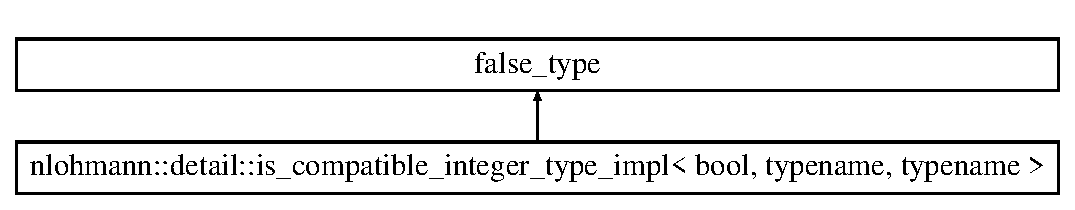
\includegraphics[height=2.000000cm]{dd/d13/structnlohmann_1_1detail_1_1is__compatible__integer__type__impl}
\end{center}
\end{figure}


The documentation for this struct was generated from the following file\+:\begin{DoxyCompactItemize}
\item 
/home/mutzi/progs/linux\+\_\+workspace/alexa-\/avs-\/prototype/src/include/nlohmann\+\_\+json.\+h\end{DoxyCompactItemize}

\hypertarget{structnlohmann_1_1detail_1_1is__compatible__integer__type__impl_3_01true_00_01RealIntegerType_0064332c4ada80cab3523aebd66ccc012a}{}\section{nlohmann\+:\+:detail\+:\+:is\+\_\+compatible\+\_\+integer\+\_\+type\+\_\+impl$<$ true, Real\+Integer\+Type, Compatible\+Number\+Integer\+Type $>$ Struct Template Reference}
\label{structnlohmann_1_1detail_1_1is__compatible__integer__type__impl_3_01true_00_01RealIntegerType_0064332c4ada80cab3523aebd66ccc012a}\index{nlohmann\+::detail\+::is\+\_\+compatible\+\_\+integer\+\_\+type\+\_\+impl$<$ true, Real\+Integer\+Type, Compatible\+Number\+Integer\+Type $>$@{nlohmann\+::detail\+::is\+\_\+compatible\+\_\+integer\+\_\+type\+\_\+impl$<$ true, Real\+Integer\+Type, Compatible\+Number\+Integer\+Type $>$}}
\subsection*{Public Types}
\begin{DoxyCompactItemize}
\item 
\mbox{\Hypertarget{structnlohmann_1_1detail_1_1is__compatible__integer__type__impl_3_01true_00_01RealIntegerType_0064332c4ada80cab3523aebd66ccc012a_a1bad172320cd124997a3d68990f50a75}\label{structnlohmann_1_1detail_1_1is__compatible__integer__type__impl_3_01true_00_01RealIntegerType_0064332c4ada80cab3523aebd66ccc012a_a1bad172320cd124997a3d68990f50a75}} 
using {\bfseries Real\+Limits} = std\+::numeric\+\_\+limits$<$ Real\+Integer\+Type $>$
\item 
\mbox{\Hypertarget{structnlohmann_1_1detail_1_1is__compatible__integer__type__impl_3_01true_00_01RealIntegerType_0064332c4ada80cab3523aebd66ccc012a_a3bf8ee2f76e74f997258c9ba40c64bc4}\label{structnlohmann_1_1detail_1_1is__compatible__integer__type__impl_3_01true_00_01RealIntegerType_0064332c4ada80cab3523aebd66ccc012a_a3bf8ee2f76e74f997258c9ba40c64bc4}} 
using {\bfseries Compatible\+Limits} = std\+::numeric\+\_\+limits$<$ Compatible\+Number\+Integer\+Type $>$
\end{DoxyCompactItemize}
\subsection*{Static Public Attributes}
\begin{DoxyCompactItemize}
\item 
static constexpr auto {\bfseries value}
\end{DoxyCompactItemize}


\subsection{Member Data Documentation}
\mbox{\Hypertarget{structnlohmann_1_1detail_1_1is__compatible__integer__type__impl_3_01true_00_01RealIntegerType_0064332c4ada80cab3523aebd66ccc012a_a4c27142452b43418b1d5c0aad01bff50}\label{structnlohmann_1_1detail_1_1is__compatible__integer__type__impl_3_01true_00_01RealIntegerType_0064332c4ada80cab3523aebd66ccc012a_a4c27142452b43418b1d5c0aad01bff50}} 
\index{nlohmann\+::detail\+::is\+\_\+compatible\+\_\+integer\+\_\+type\+\_\+impl$<$ true, Real\+Integer\+Type, Compatible\+Number\+Integer\+Type $>$@{nlohmann\+::detail\+::is\+\_\+compatible\+\_\+integer\+\_\+type\+\_\+impl$<$ true, Real\+Integer\+Type, Compatible\+Number\+Integer\+Type $>$}!value@{value}}
\index{value@{value}!nlohmann\+::detail\+::is\+\_\+compatible\+\_\+integer\+\_\+type\+\_\+impl$<$ true, Real\+Integer\+Type, Compatible\+Number\+Integer\+Type $>$@{nlohmann\+::detail\+::is\+\_\+compatible\+\_\+integer\+\_\+type\+\_\+impl$<$ true, Real\+Integer\+Type, Compatible\+Number\+Integer\+Type $>$}}
\subsubsection{\texorpdfstring{value}{value}}
{\footnotesize\ttfamily template$<$typename Real\+Integer\+Type , typename Compatible\+Number\+Integer\+Type $>$ \\
constexpr auto \hyperlink{structnlohmann_1_1detail_1_1is__compatible__integer__type__impl}{nlohmann\+::detail\+::is\+\_\+compatible\+\_\+integer\+\_\+type\+\_\+impl}$<$ true, Real\+Integer\+Type, Compatible\+Number\+Integer\+Type $>$\+::value\hspace{0.3cm}{\ttfamily [static]}}

{\bfseries Initial value\+:}
\begin{DoxyCode}
=
        std::is\_constructible<RealIntegerType,
        CompatibleNumberIntegerType>::value and
        CompatibleLimits::is\_integer and
        RealLimits::is\_signed == CompatibleLimits::is\_signed
\end{DoxyCode}


The documentation for this struct was generated from the following file\+:\begin{DoxyCompactItemize}
\item 
/home/mutzi/progs/linux\+\_\+workspace/alexa-\/avs-\/prototype/src/include/nlohmann\+\_\+json.\+h\end{DoxyCompactItemize}

\hypertarget{structnlohmann_1_1detail_1_1is__compatible__object__type}{}\section{nlohmann\+:\+:detail\+:\+:is\+\_\+compatible\+\_\+object\+\_\+type$<$ Basic\+Json\+Type, Compatible\+Object\+Type $>$ Struct Template Reference}
\label{structnlohmann_1_1detail_1_1is__compatible__object__type}\index{nlohmann\+::detail\+::is\+\_\+compatible\+\_\+object\+\_\+type$<$ Basic\+Json\+Type, Compatible\+Object\+Type $>$@{nlohmann\+::detail\+::is\+\_\+compatible\+\_\+object\+\_\+type$<$ Basic\+Json\+Type, Compatible\+Object\+Type $>$}}
\subsection*{Static Public Attributes}
\begin{DoxyCompactItemize}
\item 
static auto constexpr {\bfseries value}
\end{DoxyCompactItemize}


\subsection{Member Data Documentation}
\mbox{\Hypertarget{structnlohmann_1_1detail_1_1is__compatible__object__type_a87cce7bcdcd22cc8517f171705f6a7c7}\label{structnlohmann_1_1detail_1_1is__compatible__object__type_a87cce7bcdcd22cc8517f171705f6a7c7}} 
\index{nlohmann\+::detail\+::is\+\_\+compatible\+\_\+object\+\_\+type@{nlohmann\+::detail\+::is\+\_\+compatible\+\_\+object\+\_\+type}!value@{value}}
\index{value@{value}!nlohmann\+::detail\+::is\+\_\+compatible\+\_\+object\+\_\+type@{nlohmann\+::detail\+::is\+\_\+compatible\+\_\+object\+\_\+type}}
\subsubsection{\texorpdfstring{value}{value}}
{\footnotesize\ttfamily template$<$class Basic\+Json\+Type , class Compatible\+Object\+Type $>$ \\
auto constexpr \hyperlink{structnlohmann_1_1detail_1_1is__compatible__object__type}{nlohmann\+::detail\+::is\+\_\+compatible\+\_\+object\+\_\+type}$<$ Basic\+Json\+Type, Compatible\+Object\+Type $>$\+::value\hspace{0.3cm}{\ttfamily [static]}}

{\bfseries Initial value\+:}
\begin{DoxyCode}
= is\_compatible\_object\_type\_impl <
                                  conjunction<negation<std::is\_same<void, CompatibleObjectType>>,
                                  has\_mapped\_type<CompatibleObjectType>,
                                  has\_key\_type<CompatibleObjectType>>::value,
                                  \textcolor{keyword}{typename} BasicJsonType::object\_t, CompatibleObjectType >::value
\end{DoxyCode}


The documentation for this struct was generated from the following file\+:\begin{DoxyCompactItemize}
\item 
/home/mutzi/progs/linux\+\_\+workspace/alexa-\/avs-\/prototype/src/include/nlohmann\+\_\+json.\+h\end{DoxyCompactItemize}

\hypertarget{structnlohmann_1_1detail_1_1is__compatible__object__type__impl}{}\section{nlohmann\+:\+:detail\+:\+:is\+\_\+compatible\+\_\+object\+\_\+type\+\_\+impl$<$ B, Real\+Type, Compatible\+Object\+Type $>$ Struct Template Reference}
\label{structnlohmann_1_1detail_1_1is__compatible__object__type__impl}\index{nlohmann\+::detail\+::is\+\_\+compatible\+\_\+object\+\_\+type\+\_\+impl$<$ B, Real\+Type, Compatible\+Object\+Type $>$@{nlohmann\+::detail\+::is\+\_\+compatible\+\_\+object\+\_\+type\+\_\+impl$<$ B, Real\+Type, Compatible\+Object\+Type $>$}}
Inheritance diagram for nlohmann\+:\+:detail\+:\+:is\+\_\+compatible\+\_\+object\+\_\+type\+\_\+impl$<$ B, Real\+Type, Compatible\+Object\+Type $>$\+:\begin{figure}[H]
\begin{center}
\leavevmode
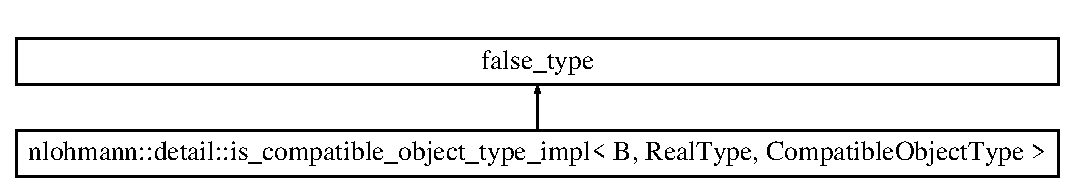
\includegraphics[height=2.000000cm]{dc/da5/structnlohmann_1_1detail_1_1is__compatible__object__type__impl}
\end{center}
\end{figure}


The documentation for this struct was generated from the following file\+:\begin{DoxyCompactItemize}
\item 
/home/mutzi/progs/linux\+\_\+workspace/alexa-\/avs-\/prototype/src/include/nlohmann\+\_\+json.\+h\end{DoxyCompactItemize}

\hypertarget{structnlohmann_1_1detail_1_1is__compatible__object__type__impl_3_01true_00_01RealType_00_01CompatibleObjectType_01_4}{}\section{nlohmann\+:\+:detail\+:\+:is\+\_\+compatible\+\_\+object\+\_\+type\+\_\+impl$<$ true, Real\+Type, Compatible\+Object\+Type $>$ Struct Template Reference}
\label{structnlohmann_1_1detail_1_1is__compatible__object__type__impl_3_01true_00_01RealType_00_01CompatibleObjectType_01_4}\index{nlohmann\+::detail\+::is\+\_\+compatible\+\_\+object\+\_\+type\+\_\+impl$<$ true, Real\+Type, Compatible\+Object\+Type $>$@{nlohmann\+::detail\+::is\+\_\+compatible\+\_\+object\+\_\+type\+\_\+impl$<$ true, Real\+Type, Compatible\+Object\+Type $>$}}
\subsection*{Static Public Attributes}
\begin{DoxyCompactItemize}
\item 
static constexpr auto {\bfseries value}
\end{DoxyCompactItemize}


\subsection{Member Data Documentation}
\mbox{\Hypertarget{structnlohmann_1_1detail_1_1is__compatible__object__type__impl_3_01true_00_01RealType_00_01CompatibleObjectType_01_4_afa131fcd3a4fc1881dd350a04589e6cf}\label{structnlohmann_1_1detail_1_1is__compatible__object__type__impl_3_01true_00_01RealType_00_01CompatibleObjectType_01_4_afa131fcd3a4fc1881dd350a04589e6cf}} 
\index{nlohmann\+::detail\+::is\+\_\+compatible\+\_\+object\+\_\+type\+\_\+impl$<$ true, Real\+Type, Compatible\+Object\+Type $>$@{nlohmann\+::detail\+::is\+\_\+compatible\+\_\+object\+\_\+type\+\_\+impl$<$ true, Real\+Type, Compatible\+Object\+Type $>$}!value@{value}}
\index{value@{value}!nlohmann\+::detail\+::is\+\_\+compatible\+\_\+object\+\_\+type\+\_\+impl$<$ true, Real\+Type, Compatible\+Object\+Type $>$@{nlohmann\+::detail\+::is\+\_\+compatible\+\_\+object\+\_\+type\+\_\+impl$<$ true, Real\+Type, Compatible\+Object\+Type $>$}}
\subsubsection{\texorpdfstring{value}{value}}
{\footnotesize\ttfamily template$<$class Real\+Type , class Compatible\+Object\+Type $>$ \\
constexpr auto \hyperlink{structnlohmann_1_1detail_1_1is__compatible__object__type__impl}{nlohmann\+::detail\+::is\+\_\+compatible\+\_\+object\+\_\+type\+\_\+impl}$<$ true, Real\+Type, Compatible\+Object\+Type $>$\+::value\hspace{0.3cm}{\ttfamily [static]}}

{\bfseries Initial value\+:}
\begin{DoxyCode}
=
        std::is\_constructible<\textcolor{keyword}{typename} RealType::key\_type,
        \textcolor{keyword}{typename} CompatibleObjectType::key\_type>::value and
        std::is\_constructible<\textcolor{keyword}{typename} RealType::mapped\_type,
        \textcolor{keyword}{typename} CompatibleObjectType::mapped\_type>::value
\end{DoxyCode}


The documentation for this struct was generated from the following file\+:\begin{DoxyCompactItemize}
\item 
/home/mutzi/progs/linux\+\_\+workspace/alexa-\/avs-\/prototype/src/include/nlohmann\+\_\+json.\+h\end{DoxyCompactItemize}

\hypertarget{classnlohmann_1_1basic__json_1_1iter__impl}{}\section{nlohmann\+:\+:basic\+\_\+json$<$ Object\+Type, Array\+Type, String\+Type, Boolean\+Type, Number\+Integer\+Type, Number\+Unsigned\+Type, Number\+Float\+Type, Allocator\+Type, J\+S\+O\+N\+Serializer $>$\+:\+:iter\+\_\+impl$<$ U $>$ Class Template Reference}
\label{classnlohmann_1_1basic__json_1_1iter__impl}\index{nlohmann\+::basic\+\_\+json$<$ Object\+Type, Array\+Type, String\+Type, Boolean\+Type, Number\+Integer\+Type, Number\+Unsigned\+Type, Number\+Float\+Type, Allocator\+Type, J\+S\+O\+N\+Serializer $>$\+::iter\+\_\+impl$<$ U $>$@{nlohmann\+::basic\+\_\+json$<$ Object\+Type, Array\+Type, String\+Type, Boolean\+Type, Number\+Integer\+Type, Number\+Unsigned\+Type, Number\+Float\+Type, Allocator\+Type, J\+S\+O\+N\+Serializer $>$\+::iter\+\_\+impl$<$ U $>$}}


a template for a random access iterator for the \hyperlink{classnlohmann_1_1basic__json}{basic\+\_\+json} class  




{\ttfamily \#include $<$nlohmann\+\_\+json.\+h$>$}

Inheritance diagram for nlohmann\+:\+:basic\+\_\+json$<$ Object\+Type, Array\+Type, String\+Type, Boolean\+Type, Number\+Integer\+Type, Number\+Unsigned\+Type, Number\+Float\+Type, Allocator\+Type, J\+S\+O\+N\+Serializer $>$\+:\+:iter\+\_\+impl$<$ U $>$\+:\begin{figure}[H]
\begin{center}
\leavevmode
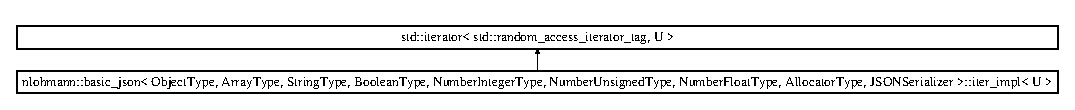
\includegraphics[height=1.033210cm]{de/d32/classnlohmann_1_1basic__json_1_1iter__impl}
\end{center}
\end{figure}
\subsection*{Public Types}
\begin{DoxyCompactItemize}
\item 
\mbox{\Hypertarget{classnlohmann_1_1basic__json_1_1iter__impl_a4d0518f3f2edae9dbaf7ef02f4f20add}\label{classnlohmann_1_1basic__json_1_1iter__impl_a4d0518f3f2edae9dbaf7ef02f4f20add}} 
using \hyperlink{classnlohmann_1_1basic__json_1_1iter__impl_a4d0518f3f2edae9dbaf7ef02f4f20add}{value\+\_\+type} = typename \hyperlink{classnlohmann_1_1basic__json_a2b3297873b70c080837e8eedc4fec32f}{basic\+\_\+json\+::value\+\_\+type}
\begin{DoxyCompactList}\small\item\em the type of the values when the iterator is dereferenced \end{DoxyCompactList}\item 
\mbox{\Hypertarget{classnlohmann_1_1basic__json_1_1iter__impl_aa3d908ee643e5938d32e5f6d261d7715}\label{classnlohmann_1_1basic__json_1_1iter__impl_aa3d908ee643e5938d32e5f6d261d7715}} 
using \hyperlink{classnlohmann_1_1basic__json_1_1iter__impl_aa3d908ee643e5938d32e5f6d261d7715}{difference\+\_\+type} = typename \hyperlink{classnlohmann_1_1basic__json_afe7c1303357e19cea9527af4e9a31d8f}{basic\+\_\+json\+::difference\+\_\+type}
\begin{DoxyCompactList}\small\item\em a type to represent differences between iterators \end{DoxyCompactList}\item 
\mbox{\Hypertarget{classnlohmann_1_1basic__json_1_1iter__impl_a3dddd7fa38b36e2531700ceb4a1ce9a8}\label{classnlohmann_1_1basic__json_1_1iter__impl_a3dddd7fa38b36e2531700ceb4a1ce9a8}} 
using \hyperlink{classnlohmann_1_1basic__json_1_1iter__impl_a3dddd7fa38b36e2531700ceb4a1ce9a8}{pointer} = typename std\+::conditional$<$ std\+::is\+\_\+const$<$ U $>$\+::\hyperlink{classnlohmann_1_1basic__json_1_1iter__impl_a92e849ca687355935c02f492be936b68}{value}, typename \hyperlink{classnlohmann_1_1basic__json_aff3d5cd2a75612364b888d8693231b58}{basic\+\_\+json\+::const\+\_\+pointer}, typename \hyperlink{classnlohmann_1_1basic__json_aefee1f777198c68724bd127e0c8abbe4}{basic\+\_\+json\+::pointer} $>$\+::\hyperlink{classnlohmann_1_1basic__json_a2b2d781d7f2a4ee41bc0016e931cadf7}{type}
\begin{DoxyCompactList}\small\item\em defines a pointer to the type iterated over (value\+\_\+type) \end{DoxyCompactList}\item 
\mbox{\Hypertarget{classnlohmann_1_1basic__json_1_1iter__impl_ae09599e9cb4a947020a0265c0c4f3d5e}\label{classnlohmann_1_1basic__json_1_1iter__impl_ae09599e9cb4a947020a0265c0c4f3d5e}} 
using \hyperlink{classnlohmann_1_1basic__json_1_1iter__impl_ae09599e9cb4a947020a0265c0c4f3d5e}{reference} = typename std\+::conditional$<$ std\+::is\+\_\+const$<$ U $>$\+::\hyperlink{classnlohmann_1_1basic__json_1_1iter__impl_a92e849ca687355935c02f492be936b68}{value}, typename \hyperlink{classnlohmann_1_1basic__json_a4057c5425f4faacfe39a8046871786ca}{basic\+\_\+json\+::const\+\_\+reference}, typename \hyperlink{classnlohmann_1_1basic__json_ac6a5eddd156c776ac75ff54cfe54a5bc}{basic\+\_\+json\+::reference} $>$\+::\hyperlink{classnlohmann_1_1basic__json_a2b2d781d7f2a4ee41bc0016e931cadf7}{type}
\begin{DoxyCompactList}\small\item\em defines a reference to the type iterated over (value\+\_\+type) \end{DoxyCompactList}\item 
\mbox{\Hypertarget{classnlohmann_1_1basic__json_1_1iter__impl_adbe1b700b9cdc38f6991fc68683a9c2c}\label{classnlohmann_1_1basic__json_1_1iter__impl_adbe1b700b9cdc38f6991fc68683a9c2c}} 
using \hyperlink{classnlohmann_1_1basic__json_1_1iter__impl_adbe1b700b9cdc38f6991fc68683a9c2c}{iterator\+\_\+category} = std\+::bidirectional\+\_\+iterator\+\_\+tag
\begin{DoxyCompactList}\small\item\em the category of the iterator \end{DoxyCompactList}\end{DoxyCompactItemize}
\subsection*{Public Member Functions}
\begin{DoxyCompactItemize}
\item 
\mbox{\Hypertarget{classnlohmann_1_1basic__json_1_1iter__impl_a3e45be67e4384b3eacb72bd6147a6a91}\label{classnlohmann_1_1basic__json_1_1iter__impl_a3e45be67e4384b3eacb72bd6147a6a91}} 
\hyperlink{classnlohmann_1_1basic__json_1_1iter__impl_a3e45be67e4384b3eacb72bd6147a6a91}{iter\+\_\+impl} ()=default
\begin{DoxyCompactList}\small\item\em default constructor \end{DoxyCompactList}\item 
\hyperlink{classnlohmann_1_1basic__json_1_1iter__impl_aa496f5348569e75d65592f25e1664770}{iter\+\_\+impl} (\hyperlink{classnlohmann_1_1basic__json_1_1iter__impl_a3dddd7fa38b36e2531700ceb4a1ce9a8}{pointer} \hyperlink{classnlohmann_1_1basic__json_a9f42ee7d10eee2d5a73fd94ca7f767ca}{object}) noexcept
\begin{DoxyCompactList}\small\item\em constructor for a given J\+S\+ON instance \end{DoxyCompactList}\item 
\mbox{\Hypertarget{classnlohmann_1_1basic__json_1_1iter__impl_af1963645f99993ac5d0d2f8516e07212}\label{classnlohmann_1_1basic__json_1_1iter__impl_af1963645f99993ac5d0d2f8516e07212}} 
{\bfseries operator const\+\_\+iterator} () const
\item 
\hyperlink{classnlohmann_1_1basic__json_1_1iter__impl_a94c010c069b5aed9e064e0579eac9a64}{iter\+\_\+impl} (const \hyperlink{classnlohmann_1_1basic__json_1_1iter__impl}{iter\+\_\+impl} \&other) noexcept
\begin{DoxyCompactList}\small\item\em copy constructor \end{DoxyCompactList}\item 
\hyperlink{classnlohmann_1_1basic__json_1_1iter__impl}{iter\+\_\+impl} \& \hyperlink{classnlohmann_1_1basic__json_1_1iter__impl_a083d9d5465de7ddfb6108f404ce54be3}{operator=} (\hyperlink{classnlohmann_1_1basic__json_1_1iter__impl}{iter\+\_\+impl} other) noexcept(std\+::is\+\_\+nothrow\+\_\+move\+\_\+constructible$<$ \hyperlink{classnlohmann_1_1basic__json_1_1iter__impl_a3dddd7fa38b36e2531700ceb4a1ce9a8}{pointer} $>$\+::\hyperlink{classnlohmann_1_1basic__json_1_1iter__impl_a92e849ca687355935c02f492be936b68}{value} and std\+::is\+\_\+nothrow\+\_\+move\+\_\+assignable$<$ \hyperlink{classnlohmann_1_1basic__json_1_1iter__impl_a3dddd7fa38b36e2531700ceb4a1ce9a8}{pointer} $>$\+::\hyperlink{classnlohmann_1_1basic__json_1_1iter__impl_a92e849ca687355935c02f492be936b68}{value} and std\+::is\+\_\+nothrow\+\_\+move\+\_\+constructible$<$ internal\+\_\+iterator $>$\+::\hyperlink{classnlohmann_1_1basic__json_1_1iter__impl_a92e849ca687355935c02f492be936b68}{value} and std\+::is\+\_\+nothrow\+\_\+move\+\_\+assignable$<$ internal\+\_\+iterator $>$\+::\hyperlink{classnlohmann_1_1basic__json_1_1iter__impl_a92e849ca687355935c02f492be936b68}{value})
\begin{DoxyCompactList}\small\item\em copy assignment \end{DoxyCompactList}\item 
\hyperlink{classnlohmann_1_1basic__json_1_1iter__impl_ae09599e9cb4a947020a0265c0c4f3d5e}{reference} \hyperlink{classnlohmann_1_1basic__json_1_1iter__impl_ae0a628811b09b9adea6d68c3a5c4ca2a}{operator$\ast$} () const
\begin{DoxyCompactList}\small\item\em return a reference to the value pointed to by the iterator \end{DoxyCompactList}\item 
\hyperlink{classnlohmann_1_1basic__json_1_1iter__impl_a3dddd7fa38b36e2531700ceb4a1ce9a8}{pointer} \hyperlink{classnlohmann_1_1basic__json_1_1iter__impl_afd0d209ef3a07a8aa3ee46e03538ffa6}{operator-\/$>$} () const
\begin{DoxyCompactList}\small\item\em dereference the iterator \end{DoxyCompactList}\item 
\hyperlink{classnlohmann_1_1basic__json_1_1iter__impl}{iter\+\_\+impl} \hyperlink{classnlohmann_1_1basic__json_1_1iter__impl_a74e26f187519bc7181b825b8f38a4e93}{operator++} (int)
\begin{DoxyCompactList}\small\item\em post-\/increment (it++) \end{DoxyCompactList}\item 
\hyperlink{classnlohmann_1_1basic__json_1_1iter__impl}{iter\+\_\+impl} \& \hyperlink{classnlohmann_1_1basic__json_1_1iter__impl_a60e2723dae1c6d537fc914c664f1a81c}{operator++} ()
\begin{DoxyCompactList}\small\item\em pre-\/increment (++it) \end{DoxyCompactList}\item 
\hyperlink{classnlohmann_1_1basic__json_1_1iter__impl}{iter\+\_\+impl} \hyperlink{classnlohmann_1_1basic__json_1_1iter__impl_a0c3a102ac61d4c6f869fe9a5d065e91e}{operator-\/-\/} (int)
\begin{DoxyCompactList}\small\item\em post-\/decrement (it--) \end{DoxyCompactList}\item 
\hyperlink{classnlohmann_1_1basic__json_1_1iter__impl}{iter\+\_\+impl} \& \hyperlink{classnlohmann_1_1basic__json_1_1iter__impl_a50c5d20f733bfe2b13d67366102ba3fe}{operator-\/-\/} ()
\begin{DoxyCompactList}\small\item\em pre-\/decrement (--it) \end{DoxyCompactList}\item 
bool \hyperlink{classnlohmann_1_1basic__json_1_1iter__impl_af3beb0d08550188082ea64d8becd12fb}{operator==} (const \hyperlink{classnlohmann_1_1basic__json_1_1iter__impl}{iter\+\_\+impl} \&other) const
\begin{DoxyCompactList}\small\item\em comparison\+: equal \end{DoxyCompactList}\item 
bool \hyperlink{classnlohmann_1_1basic__json_1_1iter__impl_af6f10c91f59565b6c6e7205ab6969a89}{operator!=} (const \hyperlink{classnlohmann_1_1basic__json_1_1iter__impl}{iter\+\_\+impl} \&other) const
\begin{DoxyCompactList}\small\item\em comparison\+: not equal \end{DoxyCompactList}\item 
bool \hyperlink{classnlohmann_1_1basic__json_1_1iter__impl_a63c655881b0b7b7499a333ba77a7e4d1}{operator$<$} (const \hyperlink{classnlohmann_1_1basic__json_1_1iter__impl}{iter\+\_\+impl} \&other) const
\begin{DoxyCompactList}\small\item\em comparison\+: smaller \end{DoxyCompactList}\item 
bool \hyperlink{classnlohmann_1_1basic__json_1_1iter__impl_a5ed57d38f57f669f5788cea881772403}{operator$<$=} (const \hyperlink{classnlohmann_1_1basic__json_1_1iter__impl}{iter\+\_\+impl} \&other) const
\begin{DoxyCompactList}\small\item\em comparison\+: less than or equal \end{DoxyCompactList}\item 
bool \hyperlink{classnlohmann_1_1basic__json_1_1iter__impl_ae6c8e672ff064e0b92073b4dd939ada6}{operator$>$} (const \hyperlink{classnlohmann_1_1basic__json_1_1iter__impl}{iter\+\_\+impl} \&other) const
\begin{DoxyCompactList}\small\item\em comparison\+: greater than \end{DoxyCompactList}\item 
bool \hyperlink{classnlohmann_1_1basic__json_1_1iter__impl_a53a239bddcbd557f335d275c806535c1}{operator$>$=} (const \hyperlink{classnlohmann_1_1basic__json_1_1iter__impl}{iter\+\_\+impl} \&other) const
\begin{DoxyCompactList}\small\item\em comparison\+: greater than or equal \end{DoxyCompactList}\item 
\hyperlink{classnlohmann_1_1basic__json_1_1iter__impl}{iter\+\_\+impl} \& \hyperlink{classnlohmann_1_1basic__json_1_1iter__impl_a170970e99b7a6d124da0fffa4cb76dba}{operator+=} (\hyperlink{classnlohmann_1_1basic__json_1_1iter__impl_aa3d908ee643e5938d32e5f6d261d7715}{difference\+\_\+type} i)
\begin{DoxyCompactList}\small\item\em add to iterator \end{DoxyCompactList}\item 
\hyperlink{classnlohmann_1_1basic__json_1_1iter__impl}{iter\+\_\+impl} \& \hyperlink{classnlohmann_1_1basic__json_1_1iter__impl_a9fd84e884e8474c000dc966d331a4854}{operator-\/=} (\hyperlink{classnlohmann_1_1basic__json_1_1iter__impl_aa3d908ee643e5938d32e5f6d261d7715}{difference\+\_\+type} i)
\begin{DoxyCompactList}\small\item\em subtract from iterator \end{DoxyCompactList}\item 
\hyperlink{classnlohmann_1_1basic__json_1_1iter__impl}{iter\+\_\+impl} \hyperlink{classnlohmann_1_1basic__json_1_1iter__impl_a3b4cd7db9a93609f8e05f1759d38d633}{operator+} (\hyperlink{classnlohmann_1_1basic__json_1_1iter__impl_aa3d908ee643e5938d32e5f6d261d7715}{difference\+\_\+type} i)
\begin{DoxyCompactList}\small\item\em add to iterator \end{DoxyCompactList}\item 
\hyperlink{classnlohmann_1_1basic__json_1_1iter__impl}{iter\+\_\+impl} \hyperlink{classnlohmann_1_1basic__json_1_1iter__impl_a926f2f9189403e72e4f694a06d4d021a}{operator-\/} (\hyperlink{classnlohmann_1_1basic__json_1_1iter__impl_aa3d908ee643e5938d32e5f6d261d7715}{difference\+\_\+type} i)
\begin{DoxyCompactList}\small\item\em subtract from iterator \end{DoxyCompactList}\item 
\hyperlink{classnlohmann_1_1basic__json_1_1iter__impl_aa3d908ee643e5938d32e5f6d261d7715}{difference\+\_\+type} \hyperlink{classnlohmann_1_1basic__json_1_1iter__impl_a3bedce4ada748251e86c7924be54e210}{operator-\/} (const \hyperlink{classnlohmann_1_1basic__json_1_1iter__impl}{iter\+\_\+impl} \&other) const
\begin{DoxyCompactList}\small\item\em return difference \end{DoxyCompactList}\item 
\hyperlink{classnlohmann_1_1basic__json_1_1iter__impl_ae09599e9cb4a947020a0265c0c4f3d5e}{reference} \hyperlink{classnlohmann_1_1basic__json_1_1iter__impl_ab58eb87c2362183da21c70be74c2b38c}{operator\mbox{[}$\,$\mbox{]}} (\hyperlink{classnlohmann_1_1basic__json_1_1iter__impl_aa3d908ee643e5938d32e5f6d261d7715}{difference\+\_\+type} n) const
\begin{DoxyCompactList}\small\item\em access to successor \end{DoxyCompactList}\item 
object\+\_\+t\+::key\+\_\+type \hyperlink{classnlohmann_1_1basic__json_1_1iter__impl_a030a45b63b70e12b18ad4f6c1c4f1239}{key} () const
\begin{DoxyCompactList}\small\item\em return the key of an object iterator \end{DoxyCompactList}\item 
\hyperlink{classnlohmann_1_1basic__json_1_1iter__impl_ae09599e9cb4a947020a0265c0c4f3d5e}{reference} \hyperlink{classnlohmann_1_1basic__json_1_1iter__impl_a92e849ca687355935c02f492be936b68}{value} () const
\begin{DoxyCompactList}\small\item\em return the value of an iterator \end{DoxyCompactList}\end{DoxyCompactItemize}
\subsection*{Friends}
\begin{DoxyCompactItemize}
\item 
\mbox{\Hypertarget{classnlohmann_1_1basic__json_1_1iter__impl_ada3100cdb8700566051828f1355fa745}\label{classnlohmann_1_1basic__json_1_1iter__impl_ada3100cdb8700566051828f1355fa745}} 
class \hyperlink{classnlohmann_1_1basic__json_1_1iter__impl_ada3100cdb8700566051828f1355fa745}{basic\+\_\+json}
\begin{DoxyCompactList}\small\item\em allow \hyperlink{classnlohmann_1_1basic__json}{basic\+\_\+json} to access private members \end{DoxyCompactList}\end{DoxyCompactItemize}


\subsection{Detailed Description}
\subsubsection*{template$<$template$<$ typename U, typename V, typename... Args $>$ class Object\+Type = std\+::map, template$<$ typename U, typename... Args $>$ class Array\+Type = std\+::vector, class String\+Type = std\+::string, class Boolean\+Type = bool, class Number\+Integer\+Type = std\+::int64\+\_\+t, class Number\+Unsigned\+Type = std\+::uint64\+\_\+t, class Number\+Float\+Type = double, template$<$ typename U $>$ class Allocator\+Type = std\+::allocator, template$<$ typename T, typename S\+F\+I\+N\+A\+E=void $>$ class J\+S\+O\+N\+Serializer = adl\+\_\+serializer$>$\newline
template$<$typename U$>$\newline
class nlohmann\+::basic\+\_\+json$<$ Object\+Type, Array\+Type, String\+Type, Boolean\+Type, Number\+Integer\+Type, Number\+Unsigned\+Type, Number\+Float\+Type, Allocator\+Type, J\+S\+O\+N\+Serializer $>$\+::iter\+\_\+impl$<$ U $>$}

a template for a random access iterator for the \hyperlink{classnlohmann_1_1basic__json}{basic\+\_\+json} class 

This class implements a both iterators (iterator and const\+\_\+iterator) for the \hyperlink{classnlohmann_1_1basic__json}{basic\+\_\+json} class.

\begin{DoxyNote}{Note}
An iterator is called {\itshape initialized} when a pointer to a J\+S\+ON value has been set (e.\+g., by a constructor or a copy assignment). If the iterator is default-\/constructed, it is {\itshape uninitialized} and most methods are undefined. {\bfseries The library uses assertions to detect calls on uninitialized iterators.}
\end{DoxyNote}
The class satisfies the following concept requirements\+:
\begin{DoxyItemize}
\item \href{http://en.cppreference.com/w/cpp/concept/RandomAccessIterator}{\tt Random\+Access\+Iterator}\+: The iterator that can be moved to point (forward and backward) to any element in constant time.
\end{DoxyItemize}

\begin{DoxySince}{Since}
version 1.\+0.\+0, simplified in version 2.\+0.\+9 
\end{DoxySince}


\subsection{Constructor \& Destructor Documentation}
\mbox{\Hypertarget{classnlohmann_1_1basic__json_1_1iter__impl_aa496f5348569e75d65592f25e1664770}\label{classnlohmann_1_1basic__json_1_1iter__impl_aa496f5348569e75d65592f25e1664770}} 
\index{nlohmann\+::basic\+\_\+json\+::iter\+\_\+impl@{nlohmann\+::basic\+\_\+json\+::iter\+\_\+impl}!iter\+\_\+impl@{iter\+\_\+impl}}
\index{iter\+\_\+impl@{iter\+\_\+impl}!nlohmann\+::basic\+\_\+json\+::iter\+\_\+impl@{nlohmann\+::basic\+\_\+json\+::iter\+\_\+impl}}
\subsubsection{\texorpdfstring{iter\+\_\+impl()}{iter\_impl()}\hspace{0.1cm}{\footnotesize\ttfamily [1/2]}}
{\footnotesize\ttfamily template$<$template$<$ typename U, typename V, typename... Args $>$ class Object\+Type = std\+::map, template$<$ typename U, typename... Args $>$ class Array\+Type = std\+::vector, class String\+Type  = std\+::string, class Boolean\+Type  = bool, class Number\+Integer\+Type  = std\+::int64\+\_\+t, class Number\+Unsigned\+Type  = std\+::uint64\+\_\+t, class Number\+Float\+Type  = double, template$<$ typename U $>$ class Allocator\+Type = std\+::allocator, template$<$ typename T, typename S\+F\+I\+N\+A\+E=void $>$ class J\+S\+O\+N\+Serializer = adl\+\_\+serializer$>$ \\
template$<$typename U $>$ \\
\hyperlink{classnlohmann_1_1basic__json}{nlohmann\+::basic\+\_\+json}$<$ Object\+Type, Array\+Type, String\+Type, Boolean\+Type, Number\+Integer\+Type, Number\+Unsigned\+Type, Number\+Float\+Type, Allocator\+Type, J\+S\+O\+N\+Serializer $>$\+::\hyperlink{classnlohmann_1_1basic__json_1_1iter__impl}{iter\+\_\+impl}$<$ U $>$\+::\hyperlink{classnlohmann_1_1basic__json_1_1iter__impl}{iter\+\_\+impl} (\begin{DoxyParamCaption}\item[{\hyperlink{classnlohmann_1_1basic__json_1_1iter__impl_a3dddd7fa38b36e2531700ceb4a1ce9a8}{pointer}}]{object }\end{DoxyParamCaption})\hspace{0.3cm}{\ttfamily [inline]}, {\ttfamily [explicit]}, {\ttfamily [noexcept]}}



constructor for a given J\+S\+ON instance 


\begin{DoxyParams}[1]{Parameters}
\mbox{\tt in}  & {\em object} & pointer to a J\+S\+ON object for this iterator \\
\hline
\end{DoxyParams}
\begin{DoxyPrecond}{Precondition}
object != nullptr 
\end{DoxyPrecond}
\begin{DoxyPostcond}{Postcondition}
The iterator is initialized; i.\+e. {\ttfamily m\+\_\+object != nullptr}. 
\end{DoxyPostcond}
\mbox{\Hypertarget{classnlohmann_1_1basic__json_1_1iter__impl_a94c010c069b5aed9e064e0579eac9a64}\label{classnlohmann_1_1basic__json_1_1iter__impl_a94c010c069b5aed9e064e0579eac9a64}} 
\index{nlohmann\+::basic\+\_\+json\+::iter\+\_\+impl@{nlohmann\+::basic\+\_\+json\+::iter\+\_\+impl}!iter\+\_\+impl@{iter\+\_\+impl}}
\index{iter\+\_\+impl@{iter\+\_\+impl}!nlohmann\+::basic\+\_\+json\+::iter\+\_\+impl@{nlohmann\+::basic\+\_\+json\+::iter\+\_\+impl}}
\subsubsection{\texorpdfstring{iter\+\_\+impl()}{iter\_impl()}\hspace{0.1cm}{\footnotesize\ttfamily [2/2]}}
{\footnotesize\ttfamily template$<$template$<$ typename U, typename V, typename... Args $>$ class Object\+Type = std\+::map, template$<$ typename U, typename... Args $>$ class Array\+Type = std\+::vector, class String\+Type  = std\+::string, class Boolean\+Type  = bool, class Number\+Integer\+Type  = std\+::int64\+\_\+t, class Number\+Unsigned\+Type  = std\+::uint64\+\_\+t, class Number\+Float\+Type  = double, template$<$ typename U $>$ class Allocator\+Type = std\+::allocator, template$<$ typename T, typename S\+F\+I\+N\+A\+E=void $>$ class J\+S\+O\+N\+Serializer = adl\+\_\+serializer$>$ \\
template$<$typename U $>$ \\
\hyperlink{classnlohmann_1_1basic__json}{nlohmann\+::basic\+\_\+json}$<$ Object\+Type, Array\+Type, String\+Type, Boolean\+Type, Number\+Integer\+Type, Number\+Unsigned\+Type, Number\+Float\+Type, Allocator\+Type, J\+S\+O\+N\+Serializer $>$\+::\hyperlink{classnlohmann_1_1basic__json_1_1iter__impl}{iter\+\_\+impl}$<$ U $>$\+::\hyperlink{classnlohmann_1_1basic__json_1_1iter__impl}{iter\+\_\+impl} (\begin{DoxyParamCaption}\item[{const \hyperlink{classnlohmann_1_1basic__json_1_1iter__impl}{iter\+\_\+impl}$<$ U $>$ \&}]{other }\end{DoxyParamCaption})\hspace{0.3cm}{\ttfamily [inline]}, {\ttfamily [noexcept]}}



copy constructor 


\begin{DoxyParams}[1]{Parameters}
\mbox{\tt in}  & {\em other} & iterator to copy from \\
\hline
\end{DoxyParams}
\begin{DoxyNote}{Note}
It is not checked whether {\itshape other} is initialized. 
\end{DoxyNote}


\subsection{Member Function Documentation}
\mbox{\Hypertarget{classnlohmann_1_1basic__json_1_1iter__impl_a030a45b63b70e12b18ad4f6c1c4f1239}\label{classnlohmann_1_1basic__json_1_1iter__impl_a030a45b63b70e12b18ad4f6c1c4f1239}} 
\index{nlohmann\+::basic\+\_\+json\+::iter\+\_\+impl@{nlohmann\+::basic\+\_\+json\+::iter\+\_\+impl}!key@{key}}
\index{key@{key}!nlohmann\+::basic\+\_\+json\+::iter\+\_\+impl@{nlohmann\+::basic\+\_\+json\+::iter\+\_\+impl}}
\subsubsection{\texorpdfstring{key()}{key()}}
{\footnotesize\ttfamily template$<$template$<$ typename U, typename V, typename... Args $>$ class Object\+Type = std\+::map, template$<$ typename U, typename... Args $>$ class Array\+Type = std\+::vector, class String\+Type  = std\+::string, class Boolean\+Type  = bool, class Number\+Integer\+Type  = std\+::int64\+\_\+t, class Number\+Unsigned\+Type  = std\+::uint64\+\_\+t, class Number\+Float\+Type  = double, template$<$ typename U $>$ class Allocator\+Type = std\+::allocator, template$<$ typename T, typename S\+F\+I\+N\+A\+E=void $>$ class J\+S\+O\+N\+Serializer = adl\+\_\+serializer$>$ \\
template$<$typename U $>$ \\
object\+\_\+t\+::key\+\_\+type \hyperlink{classnlohmann_1_1basic__json}{nlohmann\+::basic\+\_\+json}$<$ Object\+Type, Array\+Type, String\+Type, Boolean\+Type, Number\+Integer\+Type, Number\+Unsigned\+Type, Number\+Float\+Type, Allocator\+Type, J\+S\+O\+N\+Serializer $>$\+::\hyperlink{classnlohmann_1_1basic__json_1_1iter__impl}{iter\+\_\+impl}$<$ U $>$\+::key (\begin{DoxyParamCaption}{ }\end{DoxyParamCaption}) const\hspace{0.3cm}{\ttfamily [inline]}}



return the key of an object iterator 

\begin{DoxyPrecond}{Precondition}
The iterator is initialized; i.\+e. {\ttfamily m\+\_\+object != nullptr}. 
\end{DoxyPrecond}
\mbox{\Hypertarget{classnlohmann_1_1basic__json_1_1iter__impl_af6f10c91f59565b6c6e7205ab6969a89}\label{classnlohmann_1_1basic__json_1_1iter__impl_af6f10c91f59565b6c6e7205ab6969a89}} 
\index{nlohmann\+::basic\+\_\+json\+::iter\+\_\+impl@{nlohmann\+::basic\+\_\+json\+::iter\+\_\+impl}!operator"!=@{operator"!=}}
\index{operator"!=@{operator"!=}!nlohmann\+::basic\+\_\+json\+::iter\+\_\+impl@{nlohmann\+::basic\+\_\+json\+::iter\+\_\+impl}}
\subsubsection{\texorpdfstring{operator"!=()}{operator!=()}}
{\footnotesize\ttfamily template$<$template$<$ typename U, typename V, typename... Args $>$ class Object\+Type = std\+::map, template$<$ typename U, typename... Args $>$ class Array\+Type = std\+::vector, class String\+Type  = std\+::string, class Boolean\+Type  = bool, class Number\+Integer\+Type  = std\+::int64\+\_\+t, class Number\+Unsigned\+Type  = std\+::uint64\+\_\+t, class Number\+Float\+Type  = double, template$<$ typename U $>$ class Allocator\+Type = std\+::allocator, template$<$ typename T, typename S\+F\+I\+N\+A\+E=void $>$ class J\+S\+O\+N\+Serializer = adl\+\_\+serializer$>$ \\
template$<$typename U $>$ \\
bool \hyperlink{classnlohmann_1_1basic__json}{nlohmann\+::basic\+\_\+json}$<$ Object\+Type, Array\+Type, String\+Type, Boolean\+Type, Number\+Integer\+Type, Number\+Unsigned\+Type, Number\+Float\+Type, Allocator\+Type, J\+S\+O\+N\+Serializer $>$\+::\hyperlink{classnlohmann_1_1basic__json_1_1iter__impl}{iter\+\_\+impl}$<$ U $>$\+::operator!= (\begin{DoxyParamCaption}\item[{const \hyperlink{classnlohmann_1_1basic__json_1_1iter__impl}{iter\+\_\+impl}$<$ U $>$ \&}]{other }\end{DoxyParamCaption}) const\hspace{0.3cm}{\ttfamily [inline]}}



comparison\+: not equal 

\begin{DoxyPrecond}{Precondition}
The iterator is initialized; i.\+e. {\ttfamily m\+\_\+object != nullptr}. 
\end{DoxyPrecond}
\mbox{\Hypertarget{classnlohmann_1_1basic__json_1_1iter__impl_ae0a628811b09b9adea6d68c3a5c4ca2a}\label{classnlohmann_1_1basic__json_1_1iter__impl_ae0a628811b09b9adea6d68c3a5c4ca2a}} 
\index{nlohmann\+::basic\+\_\+json\+::iter\+\_\+impl@{nlohmann\+::basic\+\_\+json\+::iter\+\_\+impl}!operator$\ast$@{operator$\ast$}}
\index{operator$\ast$@{operator$\ast$}!nlohmann\+::basic\+\_\+json\+::iter\+\_\+impl@{nlohmann\+::basic\+\_\+json\+::iter\+\_\+impl}}
\subsubsection{\texorpdfstring{operator$\ast$()}{operator*()}}
{\footnotesize\ttfamily template$<$template$<$ typename U, typename V, typename... Args $>$ class Object\+Type = std\+::map, template$<$ typename U, typename... Args $>$ class Array\+Type = std\+::vector, class String\+Type  = std\+::string, class Boolean\+Type  = bool, class Number\+Integer\+Type  = std\+::int64\+\_\+t, class Number\+Unsigned\+Type  = std\+::uint64\+\_\+t, class Number\+Float\+Type  = double, template$<$ typename U $>$ class Allocator\+Type = std\+::allocator, template$<$ typename T, typename S\+F\+I\+N\+A\+E=void $>$ class J\+S\+O\+N\+Serializer = adl\+\_\+serializer$>$ \\
template$<$typename U $>$ \\
\hyperlink{classnlohmann_1_1basic__json_1_1iter__impl_ae09599e9cb4a947020a0265c0c4f3d5e}{reference} \hyperlink{classnlohmann_1_1basic__json}{nlohmann\+::basic\+\_\+json}$<$ Object\+Type, Array\+Type, String\+Type, Boolean\+Type, Number\+Integer\+Type, Number\+Unsigned\+Type, Number\+Float\+Type, Allocator\+Type, J\+S\+O\+N\+Serializer $>$\+::\hyperlink{classnlohmann_1_1basic__json_1_1iter__impl}{iter\+\_\+impl}$<$ U $>$\+::operator$\ast$ (\begin{DoxyParamCaption}{ }\end{DoxyParamCaption}) const\hspace{0.3cm}{\ttfamily [inline]}}



return a reference to the value pointed to by the iterator 

\begin{DoxyPrecond}{Precondition}
The iterator is initialized; i.\+e. {\ttfamily m\+\_\+object != nullptr}. 
\end{DoxyPrecond}
\mbox{\Hypertarget{classnlohmann_1_1basic__json_1_1iter__impl_a3b4cd7db9a93609f8e05f1759d38d633}\label{classnlohmann_1_1basic__json_1_1iter__impl_a3b4cd7db9a93609f8e05f1759d38d633}} 
\index{nlohmann\+::basic\+\_\+json\+::iter\+\_\+impl@{nlohmann\+::basic\+\_\+json\+::iter\+\_\+impl}!operator+@{operator+}}
\index{operator+@{operator+}!nlohmann\+::basic\+\_\+json\+::iter\+\_\+impl@{nlohmann\+::basic\+\_\+json\+::iter\+\_\+impl}}
\subsubsection{\texorpdfstring{operator+()}{operator+()}}
{\footnotesize\ttfamily template$<$template$<$ typename U, typename V, typename... Args $>$ class Object\+Type = std\+::map, template$<$ typename U, typename... Args $>$ class Array\+Type = std\+::vector, class String\+Type  = std\+::string, class Boolean\+Type  = bool, class Number\+Integer\+Type  = std\+::int64\+\_\+t, class Number\+Unsigned\+Type  = std\+::uint64\+\_\+t, class Number\+Float\+Type  = double, template$<$ typename U $>$ class Allocator\+Type = std\+::allocator, template$<$ typename T, typename S\+F\+I\+N\+A\+E=void $>$ class J\+S\+O\+N\+Serializer = adl\+\_\+serializer$>$ \\
template$<$typename U $>$ \\
\hyperlink{classnlohmann_1_1basic__json_1_1iter__impl}{iter\+\_\+impl} \hyperlink{classnlohmann_1_1basic__json}{nlohmann\+::basic\+\_\+json}$<$ Object\+Type, Array\+Type, String\+Type, Boolean\+Type, Number\+Integer\+Type, Number\+Unsigned\+Type, Number\+Float\+Type, Allocator\+Type, J\+S\+O\+N\+Serializer $>$\+::\hyperlink{classnlohmann_1_1basic__json_1_1iter__impl}{iter\+\_\+impl}$<$ U $>$\+::operator+ (\begin{DoxyParamCaption}\item[{\hyperlink{classnlohmann_1_1basic__json_1_1iter__impl_aa3d908ee643e5938d32e5f6d261d7715}{difference\+\_\+type}}]{i }\end{DoxyParamCaption})\hspace{0.3cm}{\ttfamily [inline]}}



add to iterator 

\begin{DoxyPrecond}{Precondition}
The iterator is initialized; i.\+e. {\ttfamily m\+\_\+object != nullptr}. 
\end{DoxyPrecond}
\mbox{\Hypertarget{classnlohmann_1_1basic__json_1_1iter__impl_a74e26f187519bc7181b825b8f38a4e93}\label{classnlohmann_1_1basic__json_1_1iter__impl_a74e26f187519bc7181b825b8f38a4e93}} 
\index{nlohmann\+::basic\+\_\+json\+::iter\+\_\+impl@{nlohmann\+::basic\+\_\+json\+::iter\+\_\+impl}!operator++@{operator++}}
\index{operator++@{operator++}!nlohmann\+::basic\+\_\+json\+::iter\+\_\+impl@{nlohmann\+::basic\+\_\+json\+::iter\+\_\+impl}}
\subsubsection{\texorpdfstring{operator++()}{operator++()}\hspace{0.1cm}{\footnotesize\ttfamily [1/2]}}
{\footnotesize\ttfamily template$<$template$<$ typename U, typename V, typename... Args $>$ class Object\+Type = std\+::map, template$<$ typename U, typename... Args $>$ class Array\+Type = std\+::vector, class String\+Type  = std\+::string, class Boolean\+Type  = bool, class Number\+Integer\+Type  = std\+::int64\+\_\+t, class Number\+Unsigned\+Type  = std\+::uint64\+\_\+t, class Number\+Float\+Type  = double, template$<$ typename U $>$ class Allocator\+Type = std\+::allocator, template$<$ typename T, typename S\+F\+I\+N\+A\+E=void $>$ class J\+S\+O\+N\+Serializer = adl\+\_\+serializer$>$ \\
template$<$typename U $>$ \\
\hyperlink{classnlohmann_1_1basic__json_1_1iter__impl}{iter\+\_\+impl} \hyperlink{classnlohmann_1_1basic__json}{nlohmann\+::basic\+\_\+json}$<$ Object\+Type, Array\+Type, String\+Type, Boolean\+Type, Number\+Integer\+Type, Number\+Unsigned\+Type, Number\+Float\+Type, Allocator\+Type, J\+S\+O\+N\+Serializer $>$\+::\hyperlink{classnlohmann_1_1basic__json_1_1iter__impl}{iter\+\_\+impl}$<$ U $>$\+::operator++ (\begin{DoxyParamCaption}\item[{int}]{ }\end{DoxyParamCaption})\hspace{0.3cm}{\ttfamily [inline]}}



post-\/increment (it++) 

\begin{DoxyPrecond}{Precondition}
The iterator is initialized; i.\+e. {\ttfamily m\+\_\+object != nullptr}. 
\end{DoxyPrecond}
\mbox{\Hypertarget{classnlohmann_1_1basic__json_1_1iter__impl_a60e2723dae1c6d537fc914c664f1a81c}\label{classnlohmann_1_1basic__json_1_1iter__impl_a60e2723dae1c6d537fc914c664f1a81c}} 
\index{nlohmann\+::basic\+\_\+json\+::iter\+\_\+impl@{nlohmann\+::basic\+\_\+json\+::iter\+\_\+impl}!operator++@{operator++}}
\index{operator++@{operator++}!nlohmann\+::basic\+\_\+json\+::iter\+\_\+impl@{nlohmann\+::basic\+\_\+json\+::iter\+\_\+impl}}
\subsubsection{\texorpdfstring{operator++()}{operator++()}\hspace{0.1cm}{\footnotesize\ttfamily [2/2]}}
{\footnotesize\ttfamily template$<$template$<$ typename U, typename V, typename... Args $>$ class Object\+Type = std\+::map, template$<$ typename U, typename... Args $>$ class Array\+Type = std\+::vector, class String\+Type  = std\+::string, class Boolean\+Type  = bool, class Number\+Integer\+Type  = std\+::int64\+\_\+t, class Number\+Unsigned\+Type  = std\+::uint64\+\_\+t, class Number\+Float\+Type  = double, template$<$ typename U $>$ class Allocator\+Type = std\+::allocator, template$<$ typename T, typename S\+F\+I\+N\+A\+E=void $>$ class J\+S\+O\+N\+Serializer = adl\+\_\+serializer$>$ \\
template$<$typename U $>$ \\
\hyperlink{classnlohmann_1_1basic__json_1_1iter__impl}{iter\+\_\+impl}\& \hyperlink{classnlohmann_1_1basic__json}{nlohmann\+::basic\+\_\+json}$<$ Object\+Type, Array\+Type, String\+Type, Boolean\+Type, Number\+Integer\+Type, Number\+Unsigned\+Type, Number\+Float\+Type, Allocator\+Type, J\+S\+O\+N\+Serializer $>$\+::\hyperlink{classnlohmann_1_1basic__json_1_1iter__impl}{iter\+\_\+impl}$<$ U $>$\+::operator++ (\begin{DoxyParamCaption}{ }\end{DoxyParamCaption})\hspace{0.3cm}{\ttfamily [inline]}}



pre-\/increment (++it) 

\begin{DoxyPrecond}{Precondition}
The iterator is initialized; i.\+e. {\ttfamily m\+\_\+object != nullptr}. 
\end{DoxyPrecond}
\mbox{\Hypertarget{classnlohmann_1_1basic__json_1_1iter__impl_a170970e99b7a6d124da0fffa4cb76dba}\label{classnlohmann_1_1basic__json_1_1iter__impl_a170970e99b7a6d124da0fffa4cb76dba}} 
\index{nlohmann\+::basic\+\_\+json\+::iter\+\_\+impl@{nlohmann\+::basic\+\_\+json\+::iter\+\_\+impl}!operator+=@{operator+=}}
\index{operator+=@{operator+=}!nlohmann\+::basic\+\_\+json\+::iter\+\_\+impl@{nlohmann\+::basic\+\_\+json\+::iter\+\_\+impl}}
\subsubsection{\texorpdfstring{operator+=()}{operator+=()}}
{\footnotesize\ttfamily template$<$template$<$ typename U, typename V, typename... Args $>$ class Object\+Type = std\+::map, template$<$ typename U, typename... Args $>$ class Array\+Type = std\+::vector, class String\+Type  = std\+::string, class Boolean\+Type  = bool, class Number\+Integer\+Type  = std\+::int64\+\_\+t, class Number\+Unsigned\+Type  = std\+::uint64\+\_\+t, class Number\+Float\+Type  = double, template$<$ typename U $>$ class Allocator\+Type = std\+::allocator, template$<$ typename T, typename S\+F\+I\+N\+A\+E=void $>$ class J\+S\+O\+N\+Serializer = adl\+\_\+serializer$>$ \\
template$<$typename U $>$ \\
\hyperlink{classnlohmann_1_1basic__json_1_1iter__impl}{iter\+\_\+impl}\& \hyperlink{classnlohmann_1_1basic__json}{nlohmann\+::basic\+\_\+json}$<$ Object\+Type, Array\+Type, String\+Type, Boolean\+Type, Number\+Integer\+Type, Number\+Unsigned\+Type, Number\+Float\+Type, Allocator\+Type, J\+S\+O\+N\+Serializer $>$\+::\hyperlink{classnlohmann_1_1basic__json_1_1iter__impl}{iter\+\_\+impl}$<$ U $>$\+::operator+= (\begin{DoxyParamCaption}\item[{\hyperlink{classnlohmann_1_1basic__json_1_1iter__impl_aa3d908ee643e5938d32e5f6d261d7715}{difference\+\_\+type}}]{i }\end{DoxyParamCaption})\hspace{0.3cm}{\ttfamily [inline]}}



add to iterator 

\begin{DoxyPrecond}{Precondition}
The iterator is initialized; i.\+e. {\ttfamily m\+\_\+object != nullptr}. 
\end{DoxyPrecond}
\mbox{\Hypertarget{classnlohmann_1_1basic__json_1_1iter__impl_a926f2f9189403e72e4f694a06d4d021a}\label{classnlohmann_1_1basic__json_1_1iter__impl_a926f2f9189403e72e4f694a06d4d021a}} 
\index{nlohmann\+::basic\+\_\+json\+::iter\+\_\+impl@{nlohmann\+::basic\+\_\+json\+::iter\+\_\+impl}!operator-\/@{operator-\/}}
\index{operator-\/@{operator-\/}!nlohmann\+::basic\+\_\+json\+::iter\+\_\+impl@{nlohmann\+::basic\+\_\+json\+::iter\+\_\+impl}}
\subsubsection{\texorpdfstring{operator-\/()}{operator-()}\hspace{0.1cm}{\footnotesize\ttfamily [1/2]}}
{\footnotesize\ttfamily template$<$template$<$ typename U, typename V, typename... Args $>$ class Object\+Type = std\+::map, template$<$ typename U, typename... Args $>$ class Array\+Type = std\+::vector, class String\+Type  = std\+::string, class Boolean\+Type  = bool, class Number\+Integer\+Type  = std\+::int64\+\_\+t, class Number\+Unsigned\+Type  = std\+::uint64\+\_\+t, class Number\+Float\+Type  = double, template$<$ typename U $>$ class Allocator\+Type = std\+::allocator, template$<$ typename T, typename S\+F\+I\+N\+A\+E=void $>$ class J\+S\+O\+N\+Serializer = adl\+\_\+serializer$>$ \\
template$<$typename U $>$ \\
\hyperlink{classnlohmann_1_1basic__json_1_1iter__impl}{iter\+\_\+impl} \hyperlink{classnlohmann_1_1basic__json}{nlohmann\+::basic\+\_\+json}$<$ Object\+Type, Array\+Type, String\+Type, Boolean\+Type, Number\+Integer\+Type, Number\+Unsigned\+Type, Number\+Float\+Type, Allocator\+Type, J\+S\+O\+N\+Serializer $>$\+::\hyperlink{classnlohmann_1_1basic__json_1_1iter__impl}{iter\+\_\+impl}$<$ U $>$\+::operator-\/ (\begin{DoxyParamCaption}\item[{\hyperlink{classnlohmann_1_1basic__json_1_1iter__impl_aa3d908ee643e5938d32e5f6d261d7715}{difference\+\_\+type}}]{i }\end{DoxyParamCaption})\hspace{0.3cm}{\ttfamily [inline]}}



subtract from iterator 

\begin{DoxyPrecond}{Precondition}
The iterator is initialized; i.\+e. {\ttfamily m\+\_\+object != nullptr}. 
\end{DoxyPrecond}
\mbox{\Hypertarget{classnlohmann_1_1basic__json_1_1iter__impl_a3bedce4ada748251e86c7924be54e210}\label{classnlohmann_1_1basic__json_1_1iter__impl_a3bedce4ada748251e86c7924be54e210}} 
\index{nlohmann\+::basic\+\_\+json\+::iter\+\_\+impl@{nlohmann\+::basic\+\_\+json\+::iter\+\_\+impl}!operator-\/@{operator-\/}}
\index{operator-\/@{operator-\/}!nlohmann\+::basic\+\_\+json\+::iter\+\_\+impl@{nlohmann\+::basic\+\_\+json\+::iter\+\_\+impl}}
\subsubsection{\texorpdfstring{operator-\/()}{operator-()}\hspace{0.1cm}{\footnotesize\ttfamily [2/2]}}
{\footnotesize\ttfamily template$<$template$<$ typename U, typename V, typename... Args $>$ class Object\+Type = std\+::map, template$<$ typename U, typename... Args $>$ class Array\+Type = std\+::vector, class String\+Type  = std\+::string, class Boolean\+Type  = bool, class Number\+Integer\+Type  = std\+::int64\+\_\+t, class Number\+Unsigned\+Type  = std\+::uint64\+\_\+t, class Number\+Float\+Type  = double, template$<$ typename U $>$ class Allocator\+Type = std\+::allocator, template$<$ typename T, typename S\+F\+I\+N\+A\+E=void $>$ class J\+S\+O\+N\+Serializer = adl\+\_\+serializer$>$ \\
template$<$typename U $>$ \\
\hyperlink{classnlohmann_1_1basic__json_1_1iter__impl_aa3d908ee643e5938d32e5f6d261d7715}{difference\+\_\+type} \hyperlink{classnlohmann_1_1basic__json}{nlohmann\+::basic\+\_\+json}$<$ Object\+Type, Array\+Type, String\+Type, Boolean\+Type, Number\+Integer\+Type, Number\+Unsigned\+Type, Number\+Float\+Type, Allocator\+Type, J\+S\+O\+N\+Serializer $>$\+::\hyperlink{classnlohmann_1_1basic__json_1_1iter__impl}{iter\+\_\+impl}$<$ U $>$\+::operator-\/ (\begin{DoxyParamCaption}\item[{const \hyperlink{classnlohmann_1_1basic__json_1_1iter__impl}{iter\+\_\+impl}$<$ U $>$ \&}]{other }\end{DoxyParamCaption}) const\hspace{0.3cm}{\ttfamily [inline]}}



return difference 

\begin{DoxyPrecond}{Precondition}
The iterator is initialized; i.\+e. {\ttfamily m\+\_\+object != nullptr}. 
\end{DoxyPrecond}
\mbox{\Hypertarget{classnlohmann_1_1basic__json_1_1iter__impl_a0c3a102ac61d4c6f869fe9a5d065e91e}\label{classnlohmann_1_1basic__json_1_1iter__impl_a0c3a102ac61d4c6f869fe9a5d065e91e}} 
\index{nlohmann\+::basic\+\_\+json\+::iter\+\_\+impl@{nlohmann\+::basic\+\_\+json\+::iter\+\_\+impl}!operator-\/-\/@{operator-\/-\/}}
\index{operator-\/-\/@{operator-\/-\/}!nlohmann\+::basic\+\_\+json\+::iter\+\_\+impl@{nlohmann\+::basic\+\_\+json\+::iter\+\_\+impl}}
\subsubsection{\texorpdfstring{operator-\/-\/()}{operator--()}\hspace{0.1cm}{\footnotesize\ttfamily [1/2]}}
{\footnotesize\ttfamily template$<$template$<$ typename U, typename V, typename... Args $>$ class Object\+Type = std\+::map, template$<$ typename U, typename... Args $>$ class Array\+Type = std\+::vector, class String\+Type  = std\+::string, class Boolean\+Type  = bool, class Number\+Integer\+Type  = std\+::int64\+\_\+t, class Number\+Unsigned\+Type  = std\+::uint64\+\_\+t, class Number\+Float\+Type  = double, template$<$ typename U $>$ class Allocator\+Type = std\+::allocator, template$<$ typename T, typename S\+F\+I\+N\+A\+E=void $>$ class J\+S\+O\+N\+Serializer = adl\+\_\+serializer$>$ \\
template$<$typename U $>$ \\
\hyperlink{classnlohmann_1_1basic__json_1_1iter__impl}{iter\+\_\+impl} \hyperlink{classnlohmann_1_1basic__json}{nlohmann\+::basic\+\_\+json}$<$ Object\+Type, Array\+Type, String\+Type, Boolean\+Type, Number\+Integer\+Type, Number\+Unsigned\+Type, Number\+Float\+Type, Allocator\+Type, J\+S\+O\+N\+Serializer $>$\+::\hyperlink{classnlohmann_1_1basic__json_1_1iter__impl}{iter\+\_\+impl}$<$ U $>$\+::operator-\/-\/ (\begin{DoxyParamCaption}\item[{int}]{ }\end{DoxyParamCaption})\hspace{0.3cm}{\ttfamily [inline]}}



post-\/decrement (it--) 

\begin{DoxyPrecond}{Precondition}
The iterator is initialized; i.\+e. {\ttfamily m\+\_\+object != nullptr}. 
\end{DoxyPrecond}
\mbox{\Hypertarget{classnlohmann_1_1basic__json_1_1iter__impl_a50c5d20f733bfe2b13d67366102ba3fe}\label{classnlohmann_1_1basic__json_1_1iter__impl_a50c5d20f733bfe2b13d67366102ba3fe}} 
\index{nlohmann\+::basic\+\_\+json\+::iter\+\_\+impl@{nlohmann\+::basic\+\_\+json\+::iter\+\_\+impl}!operator-\/-\/@{operator-\/-\/}}
\index{operator-\/-\/@{operator-\/-\/}!nlohmann\+::basic\+\_\+json\+::iter\+\_\+impl@{nlohmann\+::basic\+\_\+json\+::iter\+\_\+impl}}
\subsubsection{\texorpdfstring{operator-\/-\/()}{operator--()}\hspace{0.1cm}{\footnotesize\ttfamily [2/2]}}
{\footnotesize\ttfamily template$<$template$<$ typename U, typename V, typename... Args $>$ class Object\+Type = std\+::map, template$<$ typename U, typename... Args $>$ class Array\+Type = std\+::vector, class String\+Type  = std\+::string, class Boolean\+Type  = bool, class Number\+Integer\+Type  = std\+::int64\+\_\+t, class Number\+Unsigned\+Type  = std\+::uint64\+\_\+t, class Number\+Float\+Type  = double, template$<$ typename U $>$ class Allocator\+Type = std\+::allocator, template$<$ typename T, typename S\+F\+I\+N\+A\+E=void $>$ class J\+S\+O\+N\+Serializer = adl\+\_\+serializer$>$ \\
template$<$typename U $>$ \\
\hyperlink{classnlohmann_1_1basic__json_1_1iter__impl}{iter\+\_\+impl}\& \hyperlink{classnlohmann_1_1basic__json}{nlohmann\+::basic\+\_\+json}$<$ Object\+Type, Array\+Type, String\+Type, Boolean\+Type, Number\+Integer\+Type, Number\+Unsigned\+Type, Number\+Float\+Type, Allocator\+Type, J\+S\+O\+N\+Serializer $>$\+::\hyperlink{classnlohmann_1_1basic__json_1_1iter__impl}{iter\+\_\+impl}$<$ U $>$\+::operator-\/-\/ (\begin{DoxyParamCaption}{ }\end{DoxyParamCaption})\hspace{0.3cm}{\ttfamily [inline]}}



pre-\/decrement (--it) 

\begin{DoxyPrecond}{Precondition}
The iterator is initialized; i.\+e. {\ttfamily m\+\_\+object != nullptr}. 
\end{DoxyPrecond}
\mbox{\Hypertarget{classnlohmann_1_1basic__json_1_1iter__impl_a9fd84e884e8474c000dc966d331a4854}\label{classnlohmann_1_1basic__json_1_1iter__impl_a9fd84e884e8474c000dc966d331a4854}} 
\index{nlohmann\+::basic\+\_\+json\+::iter\+\_\+impl@{nlohmann\+::basic\+\_\+json\+::iter\+\_\+impl}!operator-\/=@{operator-\/=}}
\index{operator-\/=@{operator-\/=}!nlohmann\+::basic\+\_\+json\+::iter\+\_\+impl@{nlohmann\+::basic\+\_\+json\+::iter\+\_\+impl}}
\subsubsection{\texorpdfstring{operator-\/=()}{operator-=()}}
{\footnotesize\ttfamily template$<$template$<$ typename U, typename V, typename... Args $>$ class Object\+Type = std\+::map, template$<$ typename U, typename... Args $>$ class Array\+Type = std\+::vector, class String\+Type  = std\+::string, class Boolean\+Type  = bool, class Number\+Integer\+Type  = std\+::int64\+\_\+t, class Number\+Unsigned\+Type  = std\+::uint64\+\_\+t, class Number\+Float\+Type  = double, template$<$ typename U $>$ class Allocator\+Type = std\+::allocator, template$<$ typename T, typename S\+F\+I\+N\+A\+E=void $>$ class J\+S\+O\+N\+Serializer = adl\+\_\+serializer$>$ \\
template$<$typename U $>$ \\
\hyperlink{classnlohmann_1_1basic__json_1_1iter__impl}{iter\+\_\+impl}\& \hyperlink{classnlohmann_1_1basic__json}{nlohmann\+::basic\+\_\+json}$<$ Object\+Type, Array\+Type, String\+Type, Boolean\+Type, Number\+Integer\+Type, Number\+Unsigned\+Type, Number\+Float\+Type, Allocator\+Type, J\+S\+O\+N\+Serializer $>$\+::\hyperlink{classnlohmann_1_1basic__json_1_1iter__impl}{iter\+\_\+impl}$<$ U $>$\+::operator-\/= (\begin{DoxyParamCaption}\item[{\hyperlink{classnlohmann_1_1basic__json_1_1iter__impl_aa3d908ee643e5938d32e5f6d261d7715}{difference\+\_\+type}}]{i }\end{DoxyParamCaption})\hspace{0.3cm}{\ttfamily [inline]}}



subtract from iterator 

\begin{DoxyPrecond}{Precondition}
The iterator is initialized; i.\+e. {\ttfamily m\+\_\+object != nullptr}. 
\end{DoxyPrecond}
\mbox{\Hypertarget{classnlohmann_1_1basic__json_1_1iter__impl_afd0d209ef3a07a8aa3ee46e03538ffa6}\label{classnlohmann_1_1basic__json_1_1iter__impl_afd0d209ef3a07a8aa3ee46e03538ffa6}} 
\index{nlohmann\+::basic\+\_\+json\+::iter\+\_\+impl@{nlohmann\+::basic\+\_\+json\+::iter\+\_\+impl}!operator-\/$>$@{operator-\/$>$}}
\index{operator-\/$>$@{operator-\/$>$}!nlohmann\+::basic\+\_\+json\+::iter\+\_\+impl@{nlohmann\+::basic\+\_\+json\+::iter\+\_\+impl}}
\subsubsection{\texorpdfstring{operator-\/$>$()}{operator->()}}
{\footnotesize\ttfamily template$<$template$<$ typename U, typename V, typename... Args $>$ class Object\+Type = std\+::map, template$<$ typename U, typename... Args $>$ class Array\+Type = std\+::vector, class String\+Type  = std\+::string, class Boolean\+Type  = bool, class Number\+Integer\+Type  = std\+::int64\+\_\+t, class Number\+Unsigned\+Type  = std\+::uint64\+\_\+t, class Number\+Float\+Type  = double, template$<$ typename U $>$ class Allocator\+Type = std\+::allocator, template$<$ typename T, typename S\+F\+I\+N\+A\+E=void $>$ class J\+S\+O\+N\+Serializer = adl\+\_\+serializer$>$ \\
template$<$typename U $>$ \\
\hyperlink{classnlohmann_1_1basic__json_1_1iter__impl_a3dddd7fa38b36e2531700ceb4a1ce9a8}{pointer} \hyperlink{classnlohmann_1_1basic__json}{nlohmann\+::basic\+\_\+json}$<$ Object\+Type, Array\+Type, String\+Type, Boolean\+Type, Number\+Integer\+Type, Number\+Unsigned\+Type, Number\+Float\+Type, Allocator\+Type, J\+S\+O\+N\+Serializer $>$\+::\hyperlink{classnlohmann_1_1basic__json_1_1iter__impl}{iter\+\_\+impl}$<$ U $>$\+::operator-\/$>$ (\begin{DoxyParamCaption}{ }\end{DoxyParamCaption}) const\hspace{0.3cm}{\ttfamily [inline]}}



dereference the iterator 

\begin{DoxyPrecond}{Precondition}
The iterator is initialized; i.\+e. {\ttfamily m\+\_\+object != nullptr}. 
\end{DoxyPrecond}
\mbox{\Hypertarget{classnlohmann_1_1basic__json_1_1iter__impl_a63c655881b0b7b7499a333ba77a7e4d1}\label{classnlohmann_1_1basic__json_1_1iter__impl_a63c655881b0b7b7499a333ba77a7e4d1}} 
\index{nlohmann\+::basic\+\_\+json\+::iter\+\_\+impl@{nlohmann\+::basic\+\_\+json\+::iter\+\_\+impl}!operator$<$@{operator$<$}}
\index{operator$<$@{operator$<$}!nlohmann\+::basic\+\_\+json\+::iter\+\_\+impl@{nlohmann\+::basic\+\_\+json\+::iter\+\_\+impl}}
\subsubsection{\texorpdfstring{operator$<$()}{operator<()}}
{\footnotesize\ttfamily template$<$template$<$ typename U, typename V, typename... Args $>$ class Object\+Type = std\+::map, template$<$ typename U, typename... Args $>$ class Array\+Type = std\+::vector, class String\+Type  = std\+::string, class Boolean\+Type  = bool, class Number\+Integer\+Type  = std\+::int64\+\_\+t, class Number\+Unsigned\+Type  = std\+::uint64\+\_\+t, class Number\+Float\+Type  = double, template$<$ typename U $>$ class Allocator\+Type = std\+::allocator, template$<$ typename T, typename S\+F\+I\+N\+A\+E=void $>$ class J\+S\+O\+N\+Serializer = adl\+\_\+serializer$>$ \\
template$<$typename U $>$ \\
bool \hyperlink{classnlohmann_1_1basic__json}{nlohmann\+::basic\+\_\+json}$<$ Object\+Type, Array\+Type, String\+Type, Boolean\+Type, Number\+Integer\+Type, Number\+Unsigned\+Type, Number\+Float\+Type, Allocator\+Type, J\+S\+O\+N\+Serializer $>$\+::\hyperlink{classnlohmann_1_1basic__json_1_1iter__impl}{iter\+\_\+impl}$<$ U $>$\+::operator$<$ (\begin{DoxyParamCaption}\item[{const \hyperlink{classnlohmann_1_1basic__json_1_1iter__impl}{iter\+\_\+impl}$<$ U $>$ \&}]{other }\end{DoxyParamCaption}) const\hspace{0.3cm}{\ttfamily [inline]}}



comparison\+: smaller 

\begin{DoxyPrecond}{Precondition}
The iterator is initialized; i.\+e. {\ttfamily m\+\_\+object != nullptr}. 
\end{DoxyPrecond}
\mbox{\Hypertarget{classnlohmann_1_1basic__json_1_1iter__impl_a5ed57d38f57f669f5788cea881772403}\label{classnlohmann_1_1basic__json_1_1iter__impl_a5ed57d38f57f669f5788cea881772403}} 
\index{nlohmann\+::basic\+\_\+json\+::iter\+\_\+impl@{nlohmann\+::basic\+\_\+json\+::iter\+\_\+impl}!operator$<$=@{operator$<$=}}
\index{operator$<$=@{operator$<$=}!nlohmann\+::basic\+\_\+json\+::iter\+\_\+impl@{nlohmann\+::basic\+\_\+json\+::iter\+\_\+impl}}
\subsubsection{\texorpdfstring{operator$<$=()}{operator<=()}}
{\footnotesize\ttfamily template$<$template$<$ typename U, typename V, typename... Args $>$ class Object\+Type = std\+::map, template$<$ typename U, typename... Args $>$ class Array\+Type = std\+::vector, class String\+Type  = std\+::string, class Boolean\+Type  = bool, class Number\+Integer\+Type  = std\+::int64\+\_\+t, class Number\+Unsigned\+Type  = std\+::uint64\+\_\+t, class Number\+Float\+Type  = double, template$<$ typename U $>$ class Allocator\+Type = std\+::allocator, template$<$ typename T, typename S\+F\+I\+N\+A\+E=void $>$ class J\+S\+O\+N\+Serializer = adl\+\_\+serializer$>$ \\
template$<$typename U $>$ \\
bool \hyperlink{classnlohmann_1_1basic__json}{nlohmann\+::basic\+\_\+json}$<$ Object\+Type, Array\+Type, String\+Type, Boolean\+Type, Number\+Integer\+Type, Number\+Unsigned\+Type, Number\+Float\+Type, Allocator\+Type, J\+S\+O\+N\+Serializer $>$\+::\hyperlink{classnlohmann_1_1basic__json_1_1iter__impl}{iter\+\_\+impl}$<$ U $>$\+::operator$<$= (\begin{DoxyParamCaption}\item[{const \hyperlink{classnlohmann_1_1basic__json_1_1iter__impl}{iter\+\_\+impl}$<$ U $>$ \&}]{other }\end{DoxyParamCaption}) const\hspace{0.3cm}{\ttfamily [inline]}}



comparison\+: less than or equal 

\begin{DoxyPrecond}{Precondition}
The iterator is initialized; i.\+e. {\ttfamily m\+\_\+object != nullptr}. 
\end{DoxyPrecond}
\mbox{\Hypertarget{classnlohmann_1_1basic__json_1_1iter__impl_a083d9d5465de7ddfb6108f404ce54be3}\label{classnlohmann_1_1basic__json_1_1iter__impl_a083d9d5465de7ddfb6108f404ce54be3}} 
\index{nlohmann\+::basic\+\_\+json\+::iter\+\_\+impl@{nlohmann\+::basic\+\_\+json\+::iter\+\_\+impl}!operator=@{operator=}}
\index{operator=@{operator=}!nlohmann\+::basic\+\_\+json\+::iter\+\_\+impl@{nlohmann\+::basic\+\_\+json\+::iter\+\_\+impl}}
\subsubsection{\texorpdfstring{operator=()}{operator=()}}
{\footnotesize\ttfamily template$<$template$<$ typename U, typename V, typename... Args $>$ class Object\+Type = std\+::map, template$<$ typename U, typename... Args $>$ class Array\+Type = std\+::vector, class String\+Type  = std\+::string, class Boolean\+Type  = bool, class Number\+Integer\+Type  = std\+::int64\+\_\+t, class Number\+Unsigned\+Type  = std\+::uint64\+\_\+t, class Number\+Float\+Type  = double, template$<$ typename U $>$ class Allocator\+Type = std\+::allocator, template$<$ typename T, typename S\+F\+I\+N\+A\+E=void $>$ class J\+S\+O\+N\+Serializer = adl\+\_\+serializer$>$ \\
template$<$typename U $>$ \\
\hyperlink{classnlohmann_1_1basic__json_1_1iter__impl}{iter\+\_\+impl}\& \hyperlink{classnlohmann_1_1basic__json}{nlohmann\+::basic\+\_\+json}$<$ Object\+Type, Array\+Type, String\+Type, Boolean\+Type, Number\+Integer\+Type, Number\+Unsigned\+Type, Number\+Float\+Type, Allocator\+Type, J\+S\+O\+N\+Serializer $>$\+::\hyperlink{classnlohmann_1_1basic__json_1_1iter__impl}{iter\+\_\+impl}$<$ U $>$\+::operator= (\begin{DoxyParamCaption}\item[{\hyperlink{classnlohmann_1_1basic__json_1_1iter__impl}{iter\+\_\+impl}$<$ U $>$}]{other }\end{DoxyParamCaption})\hspace{0.3cm}{\ttfamily [inline]}, {\ttfamily [noexcept]}}



copy assignment 


\begin{DoxyParams}[1]{Parameters}
\mbox{\tt in,out}  & {\em other} & iterator to copy from \\
\hline
\end{DoxyParams}
\begin{DoxyNote}{Note}
It is not checked whether {\itshape other} is initialized. 
\end{DoxyNote}
\mbox{\Hypertarget{classnlohmann_1_1basic__json_1_1iter__impl_af3beb0d08550188082ea64d8becd12fb}\label{classnlohmann_1_1basic__json_1_1iter__impl_af3beb0d08550188082ea64d8becd12fb}} 
\index{nlohmann\+::basic\+\_\+json\+::iter\+\_\+impl@{nlohmann\+::basic\+\_\+json\+::iter\+\_\+impl}!operator==@{operator==}}
\index{operator==@{operator==}!nlohmann\+::basic\+\_\+json\+::iter\+\_\+impl@{nlohmann\+::basic\+\_\+json\+::iter\+\_\+impl}}
\subsubsection{\texorpdfstring{operator==()}{operator==()}}
{\footnotesize\ttfamily template$<$template$<$ typename U, typename V, typename... Args $>$ class Object\+Type = std\+::map, template$<$ typename U, typename... Args $>$ class Array\+Type = std\+::vector, class String\+Type  = std\+::string, class Boolean\+Type  = bool, class Number\+Integer\+Type  = std\+::int64\+\_\+t, class Number\+Unsigned\+Type  = std\+::uint64\+\_\+t, class Number\+Float\+Type  = double, template$<$ typename U $>$ class Allocator\+Type = std\+::allocator, template$<$ typename T, typename S\+F\+I\+N\+A\+E=void $>$ class J\+S\+O\+N\+Serializer = adl\+\_\+serializer$>$ \\
template$<$typename U $>$ \\
bool \hyperlink{classnlohmann_1_1basic__json}{nlohmann\+::basic\+\_\+json}$<$ Object\+Type, Array\+Type, String\+Type, Boolean\+Type, Number\+Integer\+Type, Number\+Unsigned\+Type, Number\+Float\+Type, Allocator\+Type, J\+S\+O\+N\+Serializer $>$\+::\hyperlink{classnlohmann_1_1basic__json_1_1iter__impl}{iter\+\_\+impl}$<$ U $>$\+::operator== (\begin{DoxyParamCaption}\item[{const \hyperlink{classnlohmann_1_1basic__json_1_1iter__impl}{iter\+\_\+impl}$<$ U $>$ \&}]{other }\end{DoxyParamCaption}) const\hspace{0.3cm}{\ttfamily [inline]}}



comparison\+: equal 

\begin{DoxyPrecond}{Precondition}
The iterator is initialized; i.\+e. {\ttfamily m\+\_\+object != nullptr}. 
\end{DoxyPrecond}
\mbox{\Hypertarget{classnlohmann_1_1basic__json_1_1iter__impl_ae6c8e672ff064e0b92073b4dd939ada6}\label{classnlohmann_1_1basic__json_1_1iter__impl_ae6c8e672ff064e0b92073b4dd939ada6}} 
\index{nlohmann\+::basic\+\_\+json\+::iter\+\_\+impl@{nlohmann\+::basic\+\_\+json\+::iter\+\_\+impl}!operator$>$@{operator$>$}}
\index{operator$>$@{operator$>$}!nlohmann\+::basic\+\_\+json\+::iter\+\_\+impl@{nlohmann\+::basic\+\_\+json\+::iter\+\_\+impl}}
\subsubsection{\texorpdfstring{operator$>$()}{operator>()}}
{\footnotesize\ttfamily template$<$template$<$ typename U, typename V, typename... Args $>$ class Object\+Type = std\+::map, template$<$ typename U, typename... Args $>$ class Array\+Type = std\+::vector, class String\+Type  = std\+::string, class Boolean\+Type  = bool, class Number\+Integer\+Type  = std\+::int64\+\_\+t, class Number\+Unsigned\+Type  = std\+::uint64\+\_\+t, class Number\+Float\+Type  = double, template$<$ typename U $>$ class Allocator\+Type = std\+::allocator, template$<$ typename T, typename S\+F\+I\+N\+A\+E=void $>$ class J\+S\+O\+N\+Serializer = adl\+\_\+serializer$>$ \\
template$<$typename U $>$ \\
bool \hyperlink{classnlohmann_1_1basic__json}{nlohmann\+::basic\+\_\+json}$<$ Object\+Type, Array\+Type, String\+Type, Boolean\+Type, Number\+Integer\+Type, Number\+Unsigned\+Type, Number\+Float\+Type, Allocator\+Type, J\+S\+O\+N\+Serializer $>$\+::\hyperlink{classnlohmann_1_1basic__json_1_1iter__impl}{iter\+\_\+impl}$<$ U $>$\+::operator$>$ (\begin{DoxyParamCaption}\item[{const \hyperlink{classnlohmann_1_1basic__json_1_1iter__impl}{iter\+\_\+impl}$<$ U $>$ \&}]{other }\end{DoxyParamCaption}) const\hspace{0.3cm}{\ttfamily [inline]}}



comparison\+: greater than 

\begin{DoxyPrecond}{Precondition}
The iterator is initialized; i.\+e. {\ttfamily m\+\_\+object != nullptr}. 
\end{DoxyPrecond}
\mbox{\Hypertarget{classnlohmann_1_1basic__json_1_1iter__impl_a53a239bddcbd557f335d275c806535c1}\label{classnlohmann_1_1basic__json_1_1iter__impl_a53a239bddcbd557f335d275c806535c1}} 
\index{nlohmann\+::basic\+\_\+json\+::iter\+\_\+impl@{nlohmann\+::basic\+\_\+json\+::iter\+\_\+impl}!operator$>$=@{operator$>$=}}
\index{operator$>$=@{operator$>$=}!nlohmann\+::basic\+\_\+json\+::iter\+\_\+impl@{nlohmann\+::basic\+\_\+json\+::iter\+\_\+impl}}
\subsubsection{\texorpdfstring{operator$>$=()}{operator>=()}}
{\footnotesize\ttfamily template$<$template$<$ typename U, typename V, typename... Args $>$ class Object\+Type = std\+::map, template$<$ typename U, typename... Args $>$ class Array\+Type = std\+::vector, class String\+Type  = std\+::string, class Boolean\+Type  = bool, class Number\+Integer\+Type  = std\+::int64\+\_\+t, class Number\+Unsigned\+Type  = std\+::uint64\+\_\+t, class Number\+Float\+Type  = double, template$<$ typename U $>$ class Allocator\+Type = std\+::allocator, template$<$ typename T, typename S\+F\+I\+N\+A\+E=void $>$ class J\+S\+O\+N\+Serializer = adl\+\_\+serializer$>$ \\
template$<$typename U $>$ \\
bool \hyperlink{classnlohmann_1_1basic__json}{nlohmann\+::basic\+\_\+json}$<$ Object\+Type, Array\+Type, String\+Type, Boolean\+Type, Number\+Integer\+Type, Number\+Unsigned\+Type, Number\+Float\+Type, Allocator\+Type, J\+S\+O\+N\+Serializer $>$\+::\hyperlink{classnlohmann_1_1basic__json_1_1iter__impl}{iter\+\_\+impl}$<$ U $>$\+::operator$>$= (\begin{DoxyParamCaption}\item[{const \hyperlink{classnlohmann_1_1basic__json_1_1iter__impl}{iter\+\_\+impl}$<$ U $>$ \&}]{other }\end{DoxyParamCaption}) const\hspace{0.3cm}{\ttfamily [inline]}}



comparison\+: greater than or equal 

\begin{DoxyPrecond}{Precondition}
The iterator is initialized; i.\+e. {\ttfamily m\+\_\+object != nullptr}. 
\end{DoxyPrecond}
\mbox{\Hypertarget{classnlohmann_1_1basic__json_1_1iter__impl_ab58eb87c2362183da21c70be74c2b38c}\label{classnlohmann_1_1basic__json_1_1iter__impl_ab58eb87c2362183da21c70be74c2b38c}} 
\index{nlohmann\+::basic\+\_\+json\+::iter\+\_\+impl@{nlohmann\+::basic\+\_\+json\+::iter\+\_\+impl}!operator\mbox{[}\mbox{]}@{operator[]}}
\index{operator\mbox{[}\mbox{]}@{operator[]}!nlohmann\+::basic\+\_\+json\+::iter\+\_\+impl@{nlohmann\+::basic\+\_\+json\+::iter\+\_\+impl}}
\subsubsection{\texorpdfstring{operator[]()}{operator[]()}}
{\footnotesize\ttfamily template$<$template$<$ typename U, typename V, typename... Args $>$ class Object\+Type = std\+::map, template$<$ typename U, typename... Args $>$ class Array\+Type = std\+::vector, class String\+Type  = std\+::string, class Boolean\+Type  = bool, class Number\+Integer\+Type  = std\+::int64\+\_\+t, class Number\+Unsigned\+Type  = std\+::uint64\+\_\+t, class Number\+Float\+Type  = double, template$<$ typename U $>$ class Allocator\+Type = std\+::allocator, template$<$ typename T, typename S\+F\+I\+N\+A\+E=void $>$ class J\+S\+O\+N\+Serializer = adl\+\_\+serializer$>$ \\
template$<$typename U $>$ \\
\hyperlink{classnlohmann_1_1basic__json_1_1iter__impl_ae09599e9cb4a947020a0265c0c4f3d5e}{reference} \hyperlink{classnlohmann_1_1basic__json}{nlohmann\+::basic\+\_\+json}$<$ Object\+Type, Array\+Type, String\+Type, Boolean\+Type, Number\+Integer\+Type, Number\+Unsigned\+Type, Number\+Float\+Type, Allocator\+Type, J\+S\+O\+N\+Serializer $>$\+::\hyperlink{classnlohmann_1_1basic__json_1_1iter__impl}{iter\+\_\+impl}$<$ U $>$\+::operator\mbox{[}$\,$\mbox{]} (\begin{DoxyParamCaption}\item[{\hyperlink{classnlohmann_1_1basic__json_1_1iter__impl_aa3d908ee643e5938d32e5f6d261d7715}{difference\+\_\+type}}]{n }\end{DoxyParamCaption}) const\hspace{0.3cm}{\ttfamily [inline]}}



access to successor 

\begin{DoxyPrecond}{Precondition}
The iterator is initialized; i.\+e. {\ttfamily m\+\_\+object != nullptr}. 
\end{DoxyPrecond}
\mbox{\Hypertarget{classnlohmann_1_1basic__json_1_1iter__impl_a92e849ca687355935c02f492be936b68}\label{classnlohmann_1_1basic__json_1_1iter__impl_a92e849ca687355935c02f492be936b68}} 
\index{nlohmann\+::basic\+\_\+json\+::iter\+\_\+impl@{nlohmann\+::basic\+\_\+json\+::iter\+\_\+impl}!value@{value}}
\index{value@{value}!nlohmann\+::basic\+\_\+json\+::iter\+\_\+impl@{nlohmann\+::basic\+\_\+json\+::iter\+\_\+impl}}
\subsubsection{\texorpdfstring{value()}{value()}}
{\footnotesize\ttfamily template$<$template$<$ typename U, typename V, typename... Args $>$ class Object\+Type = std\+::map, template$<$ typename U, typename... Args $>$ class Array\+Type = std\+::vector, class String\+Type  = std\+::string, class Boolean\+Type  = bool, class Number\+Integer\+Type  = std\+::int64\+\_\+t, class Number\+Unsigned\+Type  = std\+::uint64\+\_\+t, class Number\+Float\+Type  = double, template$<$ typename U $>$ class Allocator\+Type = std\+::allocator, template$<$ typename T, typename S\+F\+I\+N\+A\+E=void $>$ class J\+S\+O\+N\+Serializer = adl\+\_\+serializer$>$ \\
template$<$typename U $>$ \\
\hyperlink{classnlohmann_1_1basic__json_1_1iter__impl_ae09599e9cb4a947020a0265c0c4f3d5e}{reference} \hyperlink{classnlohmann_1_1basic__json}{nlohmann\+::basic\+\_\+json}$<$ Object\+Type, Array\+Type, String\+Type, Boolean\+Type, Number\+Integer\+Type, Number\+Unsigned\+Type, Number\+Float\+Type, Allocator\+Type, J\+S\+O\+N\+Serializer $>$\+::\hyperlink{classnlohmann_1_1basic__json_1_1iter__impl}{iter\+\_\+impl}$<$ U $>$\+::value (\begin{DoxyParamCaption}{ }\end{DoxyParamCaption}) const\hspace{0.3cm}{\ttfamily [inline]}}



return the value of an iterator 

\begin{DoxyPrecond}{Precondition}
The iterator is initialized; i.\+e. {\ttfamily m\+\_\+object != nullptr}. 
\end{DoxyPrecond}


The documentation for this class was generated from the following file\+:\begin{DoxyCompactItemize}
\item 
/home/mutzi/progs/linux\+\_\+workspace/alexa-\/avs-\/prototype/src/include/nlohmann\+\_\+json.\+h\end{DoxyCompactItemize}

\hypertarget{classnlohmann_1_1basic__json_1_1json__pointer}{}\section{nlohmann\+:\+:basic\+\_\+json$<$ Object\+Type, Array\+Type, String\+Type, Boolean\+Type, Number\+Integer\+Type, Number\+Unsigned\+Type, Number\+Float\+Type, Allocator\+Type, J\+S\+O\+N\+Serializer $>$\+:\+:json\+\_\+pointer Class Reference}
\label{classnlohmann_1_1basic__json_1_1json__pointer}\index{nlohmann\+::basic\+\_\+json$<$ Object\+Type, Array\+Type, String\+Type, Boolean\+Type, Number\+Integer\+Type, Number\+Unsigned\+Type, Number\+Float\+Type, Allocator\+Type, J\+S\+O\+N\+Serializer $>$\+::json\+\_\+pointer@{nlohmann\+::basic\+\_\+json$<$ Object\+Type, Array\+Type, String\+Type, Boolean\+Type, Number\+Integer\+Type, Number\+Unsigned\+Type, Number\+Float\+Type, Allocator\+Type, J\+S\+O\+N\+Serializer $>$\+::json\+\_\+pointer}}


J\+S\+ON Pointer.  




{\ttfamily \#include $<$nlohmann\+\_\+json.\+h$>$}

\subsection*{Public Member Functions}
\begin{DoxyCompactItemize}
\item 
\hyperlink{classnlohmann_1_1basic__json_1_1json__pointer_abaa66b0d30811b8a8670a673c686b75a}{json\+\_\+pointer} (const std\+::string \&s=\char`\"{}\char`\"{})
\begin{DoxyCompactList}\small\item\em create J\+S\+ON pointer \end{DoxyCompactList}\item 
std\+::string \hyperlink{classnlohmann_1_1basic__json_1_1json__pointer_adf63cdde9493796d8aa61bd948984b6d}{to\+\_\+string} () const noexcept
\begin{DoxyCompactList}\small\item\em return a string representation of the J\+S\+ON pointer \end{DoxyCompactList}\item 
\hyperlink{classnlohmann_1_1basic__json_1_1json__pointer_aa2583b66886218c1a035e3e507a5f931}{operator std\+::string} () const
\begin{DoxyCompactList}\small\item\em return a string representation of the J\+S\+ON pointer \end{DoxyCompactList}\end{DoxyCompactItemize}
\subsection*{Friends}
\begin{DoxyCompactItemize}
\item 
\mbox{\Hypertarget{classnlohmann_1_1basic__json_1_1json__pointer_ada3100cdb8700566051828f1355fa745}\label{classnlohmann_1_1basic__json_1_1json__pointer_ada3100cdb8700566051828f1355fa745}} 
class \hyperlink{classnlohmann_1_1basic__json_1_1json__pointer_ada3100cdb8700566051828f1355fa745}{basic\+\_\+json}
\begin{DoxyCompactList}\small\item\em allow \hyperlink{classnlohmann_1_1basic__json}{basic\+\_\+json} to access private members \end{DoxyCompactList}\item 
\mbox{\Hypertarget{classnlohmann_1_1basic__json_1_1json__pointer_a4667ef558c8c3f8a646bfda0c6654653}\label{classnlohmann_1_1basic__json_1_1json__pointer_a4667ef558c8c3f8a646bfda0c6654653}} 
bool {\bfseries operator==} (\hyperlink{classnlohmann_1_1basic__json_1_1json__pointer}{json\+\_\+pointer} const \&lhs, \hyperlink{classnlohmann_1_1basic__json_1_1json__pointer}{json\+\_\+pointer} const \&rhs) noexcept
\item 
\mbox{\Hypertarget{classnlohmann_1_1basic__json_1_1json__pointer_a6779edcf28e6f018a3bbb29c0b4b5e1e}\label{classnlohmann_1_1basic__json_1_1json__pointer_a6779edcf28e6f018a3bbb29c0b4b5e1e}} 
bool {\bfseries operator!=} (\hyperlink{classnlohmann_1_1basic__json_1_1json__pointer}{json\+\_\+pointer} const \&lhs, \hyperlink{classnlohmann_1_1basic__json_1_1json__pointer}{json\+\_\+pointer} const \&rhs) noexcept
\end{DoxyCompactItemize}


\subsection{Detailed Description}
\subsubsection*{template$<$template$<$ typename U, typename V, typename... Args $>$ class Object\+Type = std\+::map, template$<$ typename U, typename... Args $>$ class Array\+Type = std\+::vector, class String\+Type = std\+::string, class Boolean\+Type = bool, class Number\+Integer\+Type = std\+::int64\+\_\+t, class Number\+Unsigned\+Type = std\+::uint64\+\_\+t, class Number\+Float\+Type = double, template$<$ typename U $>$ class Allocator\+Type = std\+::allocator, template$<$ typename T, typename S\+F\+I\+N\+A\+E=void $>$ class J\+S\+O\+N\+Serializer = adl\+\_\+serializer$>$\newline
class nlohmann\+::basic\+\_\+json$<$ Object\+Type, Array\+Type, String\+Type, Boolean\+Type, Number\+Integer\+Type, Number\+Unsigned\+Type, Number\+Float\+Type, Allocator\+Type, J\+S\+O\+N\+Serializer $>$\+::json\+\_\+pointer}

J\+S\+ON Pointer. 

A J\+S\+ON pointer defines a string syntax for identifying a specific value within a J\+S\+ON document. It can be used with functions {\ttfamily at} and {\ttfamily operator\mbox{[}\mbox{]}}. Furthermore, J\+S\+ON pointers are the base for J\+S\+ON patches.

\begin{DoxySeeAlso}{See also}
\href{https://tools.ietf.org/html/rfc6901}{\tt R\+FC 6901}
\end{DoxySeeAlso}
\begin{DoxySince}{Since}
version 2.\+0.\+0 
\end{DoxySince}


\subsection{Constructor \& Destructor Documentation}
\mbox{\Hypertarget{classnlohmann_1_1basic__json_1_1json__pointer_abaa66b0d30811b8a8670a673c686b75a}\label{classnlohmann_1_1basic__json_1_1json__pointer_abaa66b0d30811b8a8670a673c686b75a}} 
\index{nlohmann\+::basic\+\_\+json\+::json\+\_\+pointer@{nlohmann\+::basic\+\_\+json\+::json\+\_\+pointer}!json\+\_\+pointer@{json\+\_\+pointer}}
\index{json\+\_\+pointer@{json\+\_\+pointer}!nlohmann\+::basic\+\_\+json\+::json\+\_\+pointer@{nlohmann\+::basic\+\_\+json\+::json\+\_\+pointer}}
\subsubsection{\texorpdfstring{json\+\_\+pointer()}{json\_pointer()}}
{\footnotesize\ttfamily template$<$template$<$ typename U, typename V, typename... Args $>$ class Object\+Type = std\+::map, template$<$ typename U, typename... Args $>$ class Array\+Type = std\+::vector, class String\+Type  = std\+::string, class Boolean\+Type  = bool, class Number\+Integer\+Type  = std\+::int64\+\_\+t, class Number\+Unsigned\+Type  = std\+::uint64\+\_\+t, class Number\+Float\+Type  = double, template$<$ typename U $>$ class Allocator\+Type = std\+::allocator, template$<$ typename T, typename S\+F\+I\+N\+A\+E=void $>$ class J\+S\+O\+N\+Serializer = adl\+\_\+serializer$>$ \\
\hyperlink{classnlohmann_1_1basic__json}{nlohmann\+::basic\+\_\+json}$<$ Object\+Type, Array\+Type, String\+Type, Boolean\+Type, Number\+Integer\+Type, Number\+Unsigned\+Type, Number\+Float\+Type, Allocator\+Type, J\+S\+O\+N\+Serializer $>$\+::json\+\_\+pointer\+::json\+\_\+pointer (\begin{DoxyParamCaption}\item[{const std\+::string \&}]{s = {\ttfamily \char`\"{}\char`\"{}} }\end{DoxyParamCaption})\hspace{0.3cm}{\ttfamily [inline]}, {\ttfamily [explicit]}}



create J\+S\+ON pointer 

Create a J\+S\+ON pointer according to the syntax described in \href{https://tools.ietf.org/html/rfc6901#section-3}{\tt Section 3 of R\+F\+C6901}.


\begin{DoxyParams}[1]{Parameters}
\mbox{\tt in}  & {\em s} & string representing the J\+S\+ON pointer; if omitted, the empty string is assumed which references the whole J\+S\+ON value\\
\hline
\end{DoxyParams}

\begin{DoxyExceptions}{Exceptions}
{\em parse\+\_\+error.\+107} & if the given J\+S\+ON pointer {\itshape s} is nonempty and does not begin with a slash ({\ttfamily /}); see example below\\
\hline
{\em parse\+\_\+error.\+108} & if a tilde ({\ttfamily $\sim$}) in the given J\+S\+ON pointer {\itshape s} is not followed by {\ttfamily 0} (representing {\ttfamily $\sim$}) or {\ttfamily 1} (representing {\ttfamily /}); see example below\\
\hline
\end{DoxyExceptions}
\{The example shows the construction several valid J\+S\+ON pointers as well as the exceptional behavior.,\hyperlink{classnlohmann_1_1basic__json_1_1json__pointer}{json\+\_\+pointer}\}

\begin{DoxySince}{Since}
version 2.\+0.\+0 
\end{DoxySince}


\subsection{Member Function Documentation}
\mbox{\Hypertarget{classnlohmann_1_1basic__json_1_1json__pointer_aa2583b66886218c1a035e3e507a5f931}\label{classnlohmann_1_1basic__json_1_1json__pointer_aa2583b66886218c1a035e3e507a5f931}} 
\index{nlohmann\+::basic\+\_\+json\+::json\+\_\+pointer@{nlohmann\+::basic\+\_\+json\+::json\+\_\+pointer}!operator std\+::string@{operator std\+::string}}
\index{operator std\+::string@{operator std\+::string}!nlohmann\+::basic\+\_\+json\+::json\+\_\+pointer@{nlohmann\+::basic\+\_\+json\+::json\+\_\+pointer}}
\subsubsection{\texorpdfstring{operator std\+::string()}{operator std::string()}}
{\footnotesize\ttfamily template$<$template$<$ typename U, typename V, typename... Args $>$ class Object\+Type = std\+::map, template$<$ typename U, typename... Args $>$ class Array\+Type = std\+::vector, class String\+Type  = std\+::string, class Boolean\+Type  = bool, class Number\+Integer\+Type  = std\+::int64\+\_\+t, class Number\+Unsigned\+Type  = std\+::uint64\+\_\+t, class Number\+Float\+Type  = double, template$<$ typename U $>$ class Allocator\+Type = std\+::allocator, template$<$ typename T, typename S\+F\+I\+N\+A\+E=void $>$ class J\+S\+O\+N\+Serializer = adl\+\_\+serializer$>$ \\
\hyperlink{classnlohmann_1_1basic__json}{nlohmann\+::basic\+\_\+json}$<$ Object\+Type, Array\+Type, String\+Type, Boolean\+Type, Number\+Integer\+Type, Number\+Unsigned\+Type, Number\+Float\+Type, Allocator\+Type, J\+S\+O\+N\+Serializer $>$\+::json\+\_\+pointer\+::operator std\+::string (\begin{DoxyParamCaption}{ }\end{DoxyParamCaption}) const\hspace{0.3cm}{\ttfamily [inline]}}



return a string representation of the J\+S\+ON pointer 

\begin{DoxyInvariant}{Invariant}
For each J\+S\+ON pointer {\ttfamily ptr}, it holds\+: 
\begin{DoxyCode}
ptr == \hyperlink{classnlohmann_1_1basic__json_1_1json__pointer_abaa66b0d30811b8a8670a673c686b75a}{json\_pointer}(ptr.to\_string());
\end{DoxyCode}

\end{DoxyInvariant}
\begin{DoxyReturn}{Returns}
a string representation of the J\+S\+ON pointer
\end{DoxyReturn}
\{The example shows the result of {\ttfamily to\+\_\+string}., json\+\_\+pointer\+\_\+\+\_\+to\+\_\+string\}

\begin{DoxySince}{Since}
version 2.\+0.\+0 
\end{DoxySince}
\mbox{\Hypertarget{classnlohmann_1_1basic__json_1_1json__pointer_adf63cdde9493796d8aa61bd948984b6d}\label{classnlohmann_1_1basic__json_1_1json__pointer_adf63cdde9493796d8aa61bd948984b6d}} 
\index{nlohmann\+::basic\+\_\+json\+::json\+\_\+pointer@{nlohmann\+::basic\+\_\+json\+::json\+\_\+pointer}!to\+\_\+string@{to\+\_\+string}}
\index{to\+\_\+string@{to\+\_\+string}!nlohmann\+::basic\+\_\+json\+::json\+\_\+pointer@{nlohmann\+::basic\+\_\+json\+::json\+\_\+pointer}}
\subsubsection{\texorpdfstring{to\+\_\+string()}{to\_string()}}
{\footnotesize\ttfamily template$<$template$<$ typename U, typename V, typename... Args $>$ class Object\+Type = std\+::map, template$<$ typename U, typename... Args $>$ class Array\+Type = std\+::vector, class String\+Type  = std\+::string, class Boolean\+Type  = bool, class Number\+Integer\+Type  = std\+::int64\+\_\+t, class Number\+Unsigned\+Type  = std\+::uint64\+\_\+t, class Number\+Float\+Type  = double, template$<$ typename U $>$ class Allocator\+Type = std\+::allocator, template$<$ typename T, typename S\+F\+I\+N\+A\+E=void $>$ class J\+S\+O\+N\+Serializer = adl\+\_\+serializer$>$ \\
std\+::string \hyperlink{classnlohmann_1_1basic__json}{nlohmann\+::basic\+\_\+json}$<$ Object\+Type, Array\+Type, String\+Type, Boolean\+Type, Number\+Integer\+Type, Number\+Unsigned\+Type, Number\+Float\+Type, Allocator\+Type, J\+S\+O\+N\+Serializer $>$\+::json\+\_\+pointer\+::to\+\_\+string (\begin{DoxyParamCaption}{ }\end{DoxyParamCaption}) const\hspace{0.3cm}{\ttfamily [inline]}, {\ttfamily [noexcept]}}



return a string representation of the J\+S\+ON pointer 

\begin{DoxyInvariant}{Invariant}
For each J\+S\+ON pointer {\ttfamily ptr}, it holds\+: 
\begin{DoxyCode}
ptr == \hyperlink{classnlohmann_1_1basic__json_1_1json__pointer_abaa66b0d30811b8a8670a673c686b75a}{json\_pointer}(ptr.to\_string());
\end{DoxyCode}

\end{DoxyInvariant}
\begin{DoxyReturn}{Returns}
a string representation of the J\+S\+ON pointer
\end{DoxyReturn}
\{The example shows the result of {\ttfamily to\+\_\+string}., json\+\_\+pointer\+\_\+\+\_\+to\+\_\+string\}

\begin{DoxySince}{Since}
version 2.\+0.\+0 
\end{DoxySince}


The documentation for this class was generated from the following file\+:\begin{DoxyCompactItemize}
\item 
/home/mutzi/progs/linux\+\_\+workspace/alexa-\/avs-\/prototype/src/include/nlohmann\+\_\+json.\+h\end{DoxyCompactItemize}

\hypertarget{classnlohmann_1_1basic__json_1_1json__reverse__iterator}{}\section{nlohmann\+:\+:basic\+\_\+json$<$ Object\+Type, Array\+Type, String\+Type, Boolean\+Type, Number\+Integer\+Type, Number\+Unsigned\+Type, Number\+Float\+Type, Allocator\+Type, J\+S\+O\+N\+Serializer $>$\+:\+:json\+\_\+reverse\+\_\+iterator$<$ Base $>$ Class Template Reference}
\label{classnlohmann_1_1basic__json_1_1json__reverse__iterator}\index{nlohmann\+::basic\+\_\+json$<$ Object\+Type, Array\+Type, String\+Type, Boolean\+Type, Number\+Integer\+Type, Number\+Unsigned\+Type, Number\+Float\+Type, Allocator\+Type, J\+S\+O\+N\+Serializer $>$\+::json\+\_\+reverse\+\_\+iterator$<$ Base $>$@{nlohmann\+::basic\+\_\+json$<$ Object\+Type, Array\+Type, String\+Type, Boolean\+Type, Number\+Integer\+Type, Number\+Unsigned\+Type, Number\+Float\+Type, Allocator\+Type, J\+S\+O\+N\+Serializer $>$\+::json\+\_\+reverse\+\_\+iterator$<$ Base $>$}}


a template for a reverse iterator class  




{\ttfamily \#include $<$nlohmann\+\_\+json.\+h$>$}

Inheritance diagram for nlohmann\+:\+:basic\+\_\+json$<$ Object\+Type, Array\+Type, String\+Type, Boolean\+Type, Number\+Integer\+Type, Number\+Unsigned\+Type, Number\+Float\+Type, Allocator\+Type, J\+S\+O\+N\+Serializer $>$\+:\+:json\+\_\+reverse\+\_\+iterator$<$ Base $>$\+:\begin{figure}[H]
\begin{center}
\leavevmode
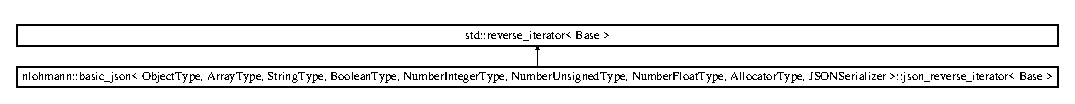
\includegraphics[height=0.950764cm]{d1/d8e/classnlohmann_1_1basic__json_1_1json__reverse__iterator}
\end{center}
\end{figure}
\subsection*{Public Types}
\begin{DoxyCompactItemize}
\item 
\mbox{\Hypertarget{classnlohmann_1_1basic__json_1_1json__reverse__iterator_a5b7f3c5d86fe89a65d9552c1cac37261}\label{classnlohmann_1_1basic__json_1_1json__reverse__iterator_a5b7f3c5d86fe89a65d9552c1cac37261}} 
using \hyperlink{classnlohmann_1_1basic__json_1_1json__reverse__iterator_a5b7f3c5d86fe89a65d9552c1cac37261}{base\+\_\+iterator} = std\+::reverse\+\_\+iterator$<$ Base $>$
\begin{DoxyCompactList}\small\item\em shortcut to the reverse iterator adaptor \end{DoxyCompactList}\item 
\mbox{\Hypertarget{classnlohmann_1_1basic__json_1_1json__reverse__iterator_ab0021ef2007fd338615360af404dcd4e}\label{classnlohmann_1_1basic__json_1_1json__reverse__iterator_ab0021ef2007fd338615360af404dcd4e}} 
using \hyperlink{classnlohmann_1_1basic__json_1_1json__reverse__iterator_ab0021ef2007fd338615360af404dcd4e}{reference} = typename Base\+::reference
\begin{DoxyCompactList}\small\item\em the reference type for the pointed-\/to element \end{DoxyCompactList}\end{DoxyCompactItemize}
\subsection*{Public Member Functions}
\begin{DoxyCompactItemize}
\item 
\mbox{\Hypertarget{classnlohmann_1_1basic__json_1_1json__reverse__iterator_a1270fe04d4801caf51e7464273305ba8}\label{classnlohmann_1_1basic__json_1_1json__reverse__iterator_a1270fe04d4801caf51e7464273305ba8}} 
\hyperlink{classnlohmann_1_1basic__json_1_1json__reverse__iterator_a1270fe04d4801caf51e7464273305ba8}{json\+\_\+reverse\+\_\+iterator} (const typename base\+\_\+iterator\+::iterator\+\_\+type \&it) noexcept
\begin{DoxyCompactList}\small\item\em create reverse iterator from iterator \end{DoxyCompactList}\item 
\mbox{\Hypertarget{classnlohmann_1_1basic__json_1_1json__reverse__iterator_af04099cd32946ab37cfa6004ad5a7863}\label{classnlohmann_1_1basic__json_1_1json__reverse__iterator_af04099cd32946ab37cfa6004ad5a7863}} 
\hyperlink{classnlohmann_1_1basic__json_1_1json__reverse__iterator_af04099cd32946ab37cfa6004ad5a7863}{json\+\_\+reverse\+\_\+iterator} (const \hyperlink{classnlohmann_1_1basic__json_1_1json__reverse__iterator_a5b7f3c5d86fe89a65d9552c1cac37261}{base\+\_\+iterator} \&it) noexcept
\begin{DoxyCompactList}\small\item\em create reverse iterator from base class \end{DoxyCompactList}\item 
\mbox{\Hypertarget{classnlohmann_1_1basic__json_1_1json__reverse__iterator_a060bdfaef94d3ca21dd6e7034980ea9c}\label{classnlohmann_1_1basic__json_1_1json__reverse__iterator_a060bdfaef94d3ca21dd6e7034980ea9c}} 
\hyperlink{classnlohmann_1_1basic__json_1_1json__reverse__iterator}{json\+\_\+reverse\+\_\+iterator} \hyperlink{classnlohmann_1_1basic__json_1_1json__reverse__iterator_a060bdfaef94d3ca21dd6e7034980ea9c}{operator++} (int)
\begin{DoxyCompactList}\small\item\em post-\/increment (it++) \end{DoxyCompactList}\item 
\mbox{\Hypertarget{classnlohmann_1_1basic__json_1_1json__reverse__iterator_aa10b55b0c57a849cfe0cba15e7818e97}\label{classnlohmann_1_1basic__json_1_1json__reverse__iterator_aa10b55b0c57a849cfe0cba15e7818e97}} 
\hyperlink{classnlohmann_1_1basic__json_1_1json__reverse__iterator}{json\+\_\+reverse\+\_\+iterator} \& \hyperlink{classnlohmann_1_1basic__json_1_1json__reverse__iterator_aa10b55b0c57a849cfe0cba15e7818e97}{operator++} ()
\begin{DoxyCompactList}\small\item\em pre-\/increment (++it) \end{DoxyCompactList}\item 
\mbox{\Hypertarget{classnlohmann_1_1basic__json_1_1json__reverse__iterator_abc37aca3fee5d832f254c94e1cd2f216}\label{classnlohmann_1_1basic__json_1_1json__reverse__iterator_abc37aca3fee5d832f254c94e1cd2f216}} 
\hyperlink{classnlohmann_1_1basic__json_1_1json__reverse__iterator}{json\+\_\+reverse\+\_\+iterator} \hyperlink{classnlohmann_1_1basic__json_1_1json__reverse__iterator_abc37aca3fee5d832f254c94e1cd2f216}{operator-\/-\/} (int)
\begin{DoxyCompactList}\small\item\em post-\/decrement (it--) \end{DoxyCompactList}\item 
\mbox{\Hypertarget{classnlohmann_1_1basic__json_1_1json__reverse__iterator_ae446e535faf6bf4a20d75ffc8525d20d}\label{classnlohmann_1_1basic__json_1_1json__reverse__iterator_ae446e535faf6bf4a20d75ffc8525d20d}} 
\hyperlink{classnlohmann_1_1basic__json_1_1json__reverse__iterator}{json\+\_\+reverse\+\_\+iterator} \& \hyperlink{classnlohmann_1_1basic__json_1_1json__reverse__iterator_ae446e535faf6bf4a20d75ffc8525d20d}{operator-\/-\/} ()
\begin{DoxyCompactList}\small\item\em pre-\/decrement (--it) \end{DoxyCompactList}\item 
\mbox{\Hypertarget{classnlohmann_1_1basic__json_1_1json__reverse__iterator_a3b884d9fc5de7013be144b304df9c068}\label{classnlohmann_1_1basic__json_1_1json__reverse__iterator_a3b884d9fc5de7013be144b304df9c068}} 
\hyperlink{classnlohmann_1_1basic__json_1_1json__reverse__iterator}{json\+\_\+reverse\+\_\+iterator} \& \hyperlink{classnlohmann_1_1basic__json_1_1json__reverse__iterator_a3b884d9fc5de7013be144b304df9c068}{operator+=} (\hyperlink{classnlohmann_1_1basic__json_afe7c1303357e19cea9527af4e9a31d8f}{difference\+\_\+type} i)
\begin{DoxyCompactList}\small\item\em add to iterator \end{DoxyCompactList}\item 
\mbox{\Hypertarget{classnlohmann_1_1basic__json_1_1json__reverse__iterator_a87a33e1b5bf42674ebe9c43ac41f8660}\label{classnlohmann_1_1basic__json_1_1json__reverse__iterator_a87a33e1b5bf42674ebe9c43ac41f8660}} 
\hyperlink{classnlohmann_1_1basic__json_1_1json__reverse__iterator}{json\+\_\+reverse\+\_\+iterator} \hyperlink{classnlohmann_1_1basic__json_1_1json__reverse__iterator_a87a33e1b5bf42674ebe9c43ac41f8660}{operator+} (\hyperlink{classnlohmann_1_1basic__json_afe7c1303357e19cea9527af4e9a31d8f}{difference\+\_\+type} i) const
\begin{DoxyCompactList}\small\item\em add to iterator \end{DoxyCompactList}\item 
\mbox{\Hypertarget{classnlohmann_1_1basic__json_1_1json__reverse__iterator_a99b0f5e39f0edc9311e28d06e4f28db8}\label{classnlohmann_1_1basic__json_1_1json__reverse__iterator_a99b0f5e39f0edc9311e28d06e4f28db8}} 
\hyperlink{classnlohmann_1_1basic__json_1_1json__reverse__iterator}{json\+\_\+reverse\+\_\+iterator} \hyperlink{classnlohmann_1_1basic__json_1_1json__reverse__iterator_a99b0f5e39f0edc9311e28d06e4f28db8}{operator-\/} (\hyperlink{classnlohmann_1_1basic__json_afe7c1303357e19cea9527af4e9a31d8f}{difference\+\_\+type} i) const
\begin{DoxyCompactList}\small\item\em subtract from iterator \end{DoxyCompactList}\item 
\mbox{\Hypertarget{classnlohmann_1_1basic__json_1_1json__reverse__iterator_a344164ae696f1c5e672d1e7d3ac20fd9}\label{classnlohmann_1_1basic__json_1_1json__reverse__iterator_a344164ae696f1c5e672d1e7d3ac20fd9}} 
\hyperlink{classnlohmann_1_1basic__json_afe7c1303357e19cea9527af4e9a31d8f}{difference\+\_\+type} \hyperlink{classnlohmann_1_1basic__json_1_1json__reverse__iterator_a344164ae696f1c5e672d1e7d3ac20fd9}{operator-\/} (const \hyperlink{classnlohmann_1_1basic__json_1_1json__reverse__iterator}{json\+\_\+reverse\+\_\+iterator} \&other) const
\begin{DoxyCompactList}\small\item\em return difference \end{DoxyCompactList}\item 
\mbox{\Hypertarget{classnlohmann_1_1basic__json_1_1json__reverse__iterator_af4879af64a0f24bd308b13b859808f84}\label{classnlohmann_1_1basic__json_1_1json__reverse__iterator_af4879af64a0f24bd308b13b859808f84}} 
\hyperlink{classnlohmann_1_1basic__json_1_1json__reverse__iterator_ab0021ef2007fd338615360af404dcd4e}{reference} \hyperlink{classnlohmann_1_1basic__json_1_1json__reverse__iterator_af4879af64a0f24bd308b13b859808f84}{operator\mbox{[}$\,$\mbox{]}} (\hyperlink{classnlohmann_1_1basic__json_afe7c1303357e19cea9527af4e9a31d8f}{difference\+\_\+type} n) const
\begin{DoxyCompactList}\small\item\em access to successor \end{DoxyCompactList}\item 
\mbox{\Hypertarget{classnlohmann_1_1basic__json_1_1json__reverse__iterator_a26c551e1cee90ee52be00b5165804598}\label{classnlohmann_1_1basic__json_1_1json__reverse__iterator_a26c551e1cee90ee52be00b5165804598}} 
object\+\_\+t\+::key\+\_\+type \hyperlink{classnlohmann_1_1basic__json_1_1json__reverse__iterator_a26c551e1cee90ee52be00b5165804598}{key} () const
\begin{DoxyCompactList}\small\item\em return the key of an object iterator \end{DoxyCompactList}\item 
\mbox{\Hypertarget{classnlohmann_1_1basic__json_1_1json__reverse__iterator_af51506d91ecf911c97521e10a047c841}\label{classnlohmann_1_1basic__json_1_1json__reverse__iterator_af51506d91ecf911c97521e10a047c841}} 
\hyperlink{classnlohmann_1_1basic__json_1_1json__reverse__iterator_ab0021ef2007fd338615360af404dcd4e}{reference} \hyperlink{classnlohmann_1_1basic__json_1_1json__reverse__iterator_af51506d91ecf911c97521e10a047c841}{value} () const
\begin{DoxyCompactList}\small\item\em return the value of an iterator \end{DoxyCompactList}\end{DoxyCompactItemize}


\subsection{Detailed Description}
\subsubsection*{template$<$template$<$ typename U, typename V, typename... Args $>$ class Object\+Type = std\+::map, template$<$ typename U, typename... Args $>$ class Array\+Type = std\+::vector, class String\+Type = std\+::string, class Boolean\+Type = bool, class Number\+Integer\+Type = std\+::int64\+\_\+t, class Number\+Unsigned\+Type = std\+::uint64\+\_\+t, class Number\+Float\+Type = double, template$<$ typename U $>$ class Allocator\+Type = std\+::allocator, template$<$ typename T, typename S\+F\+I\+N\+A\+E=void $>$ class J\+S\+O\+N\+Serializer = adl\+\_\+serializer$>$\newline
template$<$typename Base$>$\newline
class nlohmann\+::basic\+\_\+json$<$ Object\+Type, Array\+Type, String\+Type, Boolean\+Type, Number\+Integer\+Type, Number\+Unsigned\+Type, Number\+Float\+Type, Allocator\+Type, J\+S\+O\+N\+Serializer $>$\+::json\+\_\+reverse\+\_\+iterator$<$ Base $>$}

a template for a reverse iterator class 


\begin{DoxyTemplParams}{Template Parameters}
{\em Base} & the base iterator type to reverse. Valid types are \hyperlink{classnlohmann_1_1basic__json_a099316232c76c034030a38faa6e34dca}{iterator} (to create \hyperlink{classnlohmann_1_1basic__json_ac223d5560c2b05a208c88de67376c5f2}{reverse\+\_\+iterator}) and \hyperlink{classnlohmann_1_1basic__json_a41a70cf9993951836d129bb1c2b3126a}{const\+\_\+iterator} (to create \hyperlink{classnlohmann_1_1basic__json_a72be3c24bfa24f0993d6c11af03e7404}{const\+\_\+reverse\+\_\+iterator}).\\
\hline
\end{DoxyTemplParams}
The class satisfies the following concept requirements\+:
\begin{DoxyItemize}
\item \href{http://en.cppreference.com/w/cpp/concept/RandomAccessIterator}{\tt Random\+Access\+Iterator}\+: The iterator that can be moved to point (forward and backward) to any element in constant time.
\item \href{http://en.cppreference.com/w/cpp/concept/OutputIterator}{\tt Output\+Iterator}\+: It is possible to write to the pointed-\/to element (only if {\itshape Base} is \hyperlink{classnlohmann_1_1basic__json_a099316232c76c034030a38faa6e34dca}{iterator}).
\end{DoxyItemize}

\begin{DoxySince}{Since}
version 1.\+0.\+0 
\end{DoxySince}


The documentation for this class was generated from the following file\+:\begin{DoxyCompactItemize}
\item 
/home/mutzi/progs/linux\+\_\+workspace/alexa-\/avs-\/prototype/src/include/nlohmann\+\_\+json.\+h\end{DoxyCompactItemize}

\hypertarget{classAVSJson_1_1JsonFactory}{}\section{A\+V\+S\+Json\+:\+:Json\+Factory Class Reference}
\label{classAVSJson_1_1JsonFactory}\index{A\+V\+S\+Json\+::\+Json\+Factory@{A\+V\+S\+Json\+::\+Json\+Factory}}
\subsection*{Public Member Functions}
\begin{DoxyCompactItemize}
\item 
const std\+::string \hyperlink{classAVSJson_1_1JsonFactory_a81f6e5126ee5a0fe06adfb7a2de3bde6}{create\+System\+Synchronize\+Event} (const \hyperlink{structAVSJson_1_1SynchronizeStateEvent}{Synchronize\+State\+Event} $\ast$event)
\begin{DoxyCompactList}\small\item\em Json\+Factory\+::create\+H\+T\+T\+P\+Json\+Syncstate\+Obj. \end{DoxyCompactList}\item 
const std\+::string \hyperlink{classAVSJson_1_1JsonFactory_ac87cea12e6e85b725c62a35a89816458}{create\+Speech\+Recognizer\+Event} (const \hyperlink{structAVSJson_1_1SynchronizeStateEvent}{Synchronize\+State\+Event} $\ast$event, const std\+::string \&dialog\+\_\+request\+\_\+id)
\begin{DoxyCompactList}\small\item\em Json\+Factory\+::create\+H\+T\+T\+P\+Json\+Audio\+Obj. \end{DoxyCompactList}\item 
const std\+::string \hyperlink{classAVSJson_1_1JsonFactory_a74054bd58dc43cf48d10e4e2b7dd36b8}{create\+Speech\+Synthesizer\+Start\+Event} (const std\+::string \&message\+Id, const std\+::string \&token)
\begin{DoxyCompactList}\small\item\em \hyperlink{classAVSJson_1_1JsonFactory_a74054bd58dc43cf48d10e4e2b7dd36b8}{Json\+Factory\+::create\+Speech\+Synthesizer\+Start\+Event}. \end{DoxyCompactList}\item 
const std\+::string \hyperlink{classAVSJson_1_1JsonFactory_a7eaa5203dd954ce2f2d60e3a7f3b0fb5}{create\+Speech\+Synthesizer\+Finish\+Event} (const std\+::string \&message\+Id, const std\+::string \&token)
\begin{DoxyCompactList}\small\item\em \hyperlink{classAVSJson_1_1JsonFactory_a7eaa5203dd954ce2f2d60e3a7f3b0fb5}{Json\+Factory\+::create\+Speech\+Synthesizer\+Finish\+Event}. \end{DoxyCompactList}\item 
const std\+::string \hyperlink{classAVSJson_1_1JsonFactory_a2ec0b23941d61705c3680d6017c1eb27}{create\+Set\+Alert\+Succeeded\+Event} (const std\+::string \&message\+Id, const std\+::string \&token)
\begin{DoxyCompactList}\small\item\em create\+Set\+Alert\+Succeeded\+Event \end{DoxyCompactList}\item 
const std\+::string \hyperlink{classAVSJson_1_1JsonFactory_a12b8a89030081dbfb9df43279c5fa1f0}{create\+Set\+Alert\+Failed\+Event} (const std\+::string \&message\+Id, const std\+::string \&token)
\begin{DoxyCompactList}\small\item\em create\+Set\+Alert\+Failed\+Event \end{DoxyCompactList}\item 
const std\+::string \hyperlink{classAVSJson_1_1JsonFactory_a6c03efa846b5d1cd410405d794ea292f}{create\+Delete\+Alert\+Failed\+Event} (const std\+::string \&message\+Id, const std\+::string \&token)
\begin{DoxyCompactList}\small\item\em create\+Delete\+Alert\+Failed\+Event \end{DoxyCompactList}\item 
const std\+::string \hyperlink{classAVSJson_1_1JsonFactory_af4b4bccd89a168a3ee57e73a346d5554}{create\+Alert\+Started\+Event} (const std\+::string \&message\+Id, const std\+::string \&token)
\begin{DoxyCompactList}\small\item\em create\+Alert\+Started\+Event \end{DoxyCompactList}\item 
const std\+::string \hyperlink{classAVSJson_1_1JsonFactory_a86e0cf9125314d467eda43686b5916f6}{create\+Alert\+Stopped\+Event} (const std\+::string \&message\+Id, const std\+::string \&token)
\begin{DoxyCompactList}\small\item\em create\+Alert\+Stopped\+Event \end{DoxyCompactList}\item 
const std\+::string \hyperlink{classAVSJson_1_1JsonFactory_afa1846a4bb4a30124c9bf9852c5618d7}{create\+Alert\+Entered\+Foreground\+Event} (const std\+::string \&message\+Id, const std\+::string \&token)
\begin{DoxyCompactList}\small\item\em create\+Alert\+Entered\+Foreground\+Event \end{DoxyCompactList}\item 
const std\+::string \hyperlink{classAVSJson_1_1JsonFactory_a650bd9287a8cc3975ec510f7c816c1d8}{create\+Alert\+Entered\+Background\+Event} (const std\+::string \&message\+Id, const std\+::string \&token)
\begin{DoxyCompactList}\small\item\em create\+Alert\+Entered\+Background\+Event \end{DoxyCompactList}\item 
const std\+::string \hyperlink{classAVSJson_1_1JsonFactory_a6ad69e447a84fe222b0b318cf5e1f74d}{create\+Playback\+Started\+Event} (const std\+::string \&message\+Id, const std\+::string \&token, long offset)
\begin{DoxyCompactList}\small\item\em create\+Playback\+Started\+Event \end{DoxyCompactList}\item 
\mbox{\Hypertarget{classAVSJson_1_1JsonFactory_a939227104c9aeb3bd490a7a6a3822469}\label{classAVSJson_1_1JsonFactory_a939227104c9aeb3bd490a7a6a3822469}} 
const std\+::string {\bfseries create\+Playback\+Nearly\+Finished\+Event} (const std\+::string \&message\+Id, const std\+::string \&token, long offset)
\item 
\mbox{\Hypertarget{classAVSJson_1_1JsonFactory_a32ef237f77b9065dcb711e95810522e3}\label{classAVSJson_1_1JsonFactory_a32ef237f77b9065dcb711e95810522e3}} 
const std\+::string {\bfseries create\+Progress\+Report\+Delay\+Elapsed\+Event} (const std\+::string \&message\+Id, const std\+::string \&token, long offset)
\item 
\mbox{\Hypertarget{classAVSJson_1_1JsonFactory_ad57a9016772ea36d9782544bc6e3aead}\label{classAVSJson_1_1JsonFactory_ad57a9016772ea36d9782544bc6e3aead}} 
const std\+::string {\bfseries create\+Progress\+Report\+Interval\+Elapsed\+Event} (const std\+::string \&message\+Id, const std\+::string \&token, long offset)
\item 
\mbox{\Hypertarget{classAVSJson_1_1JsonFactory_a83e17b2b8c7ff1b81118b38078339818}\label{classAVSJson_1_1JsonFactory_a83e17b2b8c7ff1b81118b38078339818}} 
const std\+::string {\bfseries create\+Playback\+Stutter\+Started\+Event} (const std\+::string \&message\+Id, const std\+::string \&token, long offset)
\item 
\mbox{\Hypertarget{classAVSJson_1_1JsonFactory_a62362b2b370767469345b9aef0ee60d3}\label{classAVSJson_1_1JsonFactory_a62362b2b370767469345b9aef0ee60d3}} 
const std\+::string {\bfseries create\+Playback\+Stutter\+Finished\+Event} (const std\+::string \&message\+Id, const std\+::string \&token, long offset)
\item 
\mbox{\Hypertarget{classAVSJson_1_1JsonFactory_a1dd6693e5aedaa6f861e940199cd7253}\label{classAVSJson_1_1JsonFactory_a1dd6693e5aedaa6f861e940199cd7253}} 
const std\+::string {\bfseries create\+Playback\+Finished\+Event} (const std\+::string \&message\+Id, const std\+::string \&token, long offset)
\item 
\mbox{\Hypertarget{classAVSJson_1_1JsonFactory_ad0bf175be488881f5c212348df49102d}\label{classAVSJson_1_1JsonFactory_ad0bf175be488881f5c212348df49102d}} 
const std\+::string {\bfseries create\+Playback\+Failed\+Event} (const std\+::string \&message\+Id, const \hyperlink{structAVSJson_1_1PayloadPlaybackFailedParam}{Payload\+Playback\+Failed\+Param} $\ast$param)
\item 
\mbox{\Hypertarget{classAVSJson_1_1JsonFactory_a47d87687e09ec597f6d59453aa5db33d}\label{classAVSJson_1_1JsonFactory_a47d87687e09ec597f6d59453aa5db33d}} 
const std\+::string {\bfseries create\+Playback\+Stopped\+Event} (const std\+::string \&message\+Id, const std\+::string \&token, long offset)
\item 
\mbox{\Hypertarget{classAVSJson_1_1JsonFactory_abbb51408dd99f7d422d5bc1fc6bae8df}\label{classAVSJson_1_1JsonFactory_abbb51408dd99f7d422d5bc1fc6bae8df}} 
const std\+::string {\bfseries create\+Playback\+Paused\+Event} (const std\+::string \&message\+Id, const std\+::string \&token, long offset)
\item 
\mbox{\Hypertarget{classAVSJson_1_1JsonFactory_a081dec302444567e76a78dba3e8a6a8a}\label{classAVSJson_1_1JsonFactory_a081dec302444567e76a78dba3e8a6a8a}} 
const std\+::string {\bfseries create\+Playback\+Resumed\+Event} (const std\+::string \&message\+Id, const std\+::string \&token, long offset)
\item 
\mbox{\Hypertarget{classAVSJson_1_1JsonFactory_a016050b46ab274d271917efb1377c509}\label{classAVSJson_1_1JsonFactory_a016050b46ab274d271917efb1377c509}} 
const std\+::string {\bfseries create\+Playback\+Queue\+Cleared\+Event} (const std\+::string \&message\+Id)
\item 
\mbox{\Hypertarget{classAVSJson_1_1JsonFactory_a90f1f7963109b1f311bd6b77ea3152b2}\label{classAVSJson_1_1JsonFactory_a90f1f7963109b1f311bd6b77ea3152b2}} 
const std\+::string {\bfseries create\+Play\+Command\+Issued\+Event} (const \hyperlink{structAVSJson_1_1SynchronizeStateEvent}{Synchronize\+State\+Event} $\ast$event, const std\+::string \&message\+Id)
\item 
\mbox{\Hypertarget{classAVSJson_1_1JsonFactory_a63aef66441b23a9a16c4302dc6bffa01}\label{classAVSJson_1_1JsonFactory_a63aef66441b23a9a16c4302dc6bffa01}} 
const std\+::string {\bfseries create\+Pause\+Command\+Issued\+Event} (const \hyperlink{structAVSJson_1_1SynchronizeStateEvent}{Synchronize\+State\+Event} $\ast$event, const std\+::string \&message\+Id)
\item 
\mbox{\Hypertarget{classAVSJson_1_1JsonFactory_a3214dad9adda71a102d1ca43ec15bbe0}\label{classAVSJson_1_1JsonFactory_a3214dad9adda71a102d1ca43ec15bbe0}} 
const std\+::string {\bfseries create\+Next\+Command\+Issued\+Event} (const \hyperlink{structAVSJson_1_1SynchronizeStateEvent}{Synchronize\+State\+Event} $\ast$event, const std\+::string \&message\+Id)
\item 
\mbox{\Hypertarget{classAVSJson_1_1JsonFactory_abaa76707ececb7ca6ae18d1011e81c70}\label{classAVSJson_1_1JsonFactory_abaa76707ececb7ca6ae18d1011e81c70}} 
const std\+::string {\bfseries create\+Previous\+Command\+Issued\+Event} (const \hyperlink{structAVSJson_1_1SynchronizeStateEvent}{Synchronize\+State\+Event} $\ast$event, const std\+::string \&message\+Id)
\item 
\mbox{\Hypertarget{classAVSJson_1_1JsonFactory_af2cf888f2e24f07cc5a4ee164db9f635}\label{classAVSJson_1_1JsonFactory_af2cf888f2e24f07cc5a4ee164db9f635}} 
const std\+::string {\bfseries create\+Volume\+Changed\+Event} (const std\+::string \&message\+Id, long volume, bool muted)
\item 
\mbox{\Hypertarget{classAVSJson_1_1JsonFactory_a7e344f50688f685c7a3401fc3af96bc8}\label{classAVSJson_1_1JsonFactory_a7e344f50688f685c7a3401fc3af96bc8}} 
const std\+::string {\bfseries create\+Mute\+Changed\+Event} (const std\+::string \&message\+Id, long volume, bool muted)
\item 
const std\+::string \hyperlink{classAVSJson_1_1JsonFactory_a0a75dcab64c23b6d7512b548eaad967f}{create\+Settings\+Update\+Event} (const std\+::string \&message\+Id, const std\+::string \&key, const std\+::string \&value)
\begin{DoxyCompactList}\small\item\em create\+Settings\+Update\+Event \end{DoxyCompactList}\end{DoxyCompactItemize}
\subsection*{Protected Member Functions}
\begin{DoxyCompactItemize}
\item 
const std\+::string \hyperlink{classAVSJson_1_1JsonFactory_aa6aab87bcc8fcb68add7dc86fac36bf0}{create\+Alerts\+Context} (const \hyperlink{structAVSJson_1_1AlertsState}{Alerts\+State} $\ast$state)
\begin{DoxyCompactList}\small\item\em \hyperlink{classAVSJson_1_1JsonFactory_aa6aab87bcc8fcb68add7dc86fac36bf0}{Json\+Factory\+::create\+Alerts\+Context}. \end{DoxyCompactList}\item 
const std\+::string \hyperlink{classAVSJson_1_1JsonFactory_afa83d7cfe2079159f3f8923d0ad82cf2}{create\+Playback\+Context} (const \hyperlink{structAVSJson_1_1PlaybackState}{Playback\+State} $\ast$state)
\begin{DoxyCompactList}\small\item\em \hyperlink{classAVSJson_1_1JsonFactory_afa83d7cfe2079159f3f8923d0ad82cf2}{Json\+Factory\+::create\+Playback\+Context}. \end{DoxyCompactList}\item 
const std\+::string \hyperlink{classAVSJson_1_1JsonFactory_af36d05a150eaccfe398f5c128298eab5}{create\+Speaker\+Context} (const \hyperlink{structAVSJson_1_1VolumeState}{Volume\+State} $\ast$state)
\begin{DoxyCompactList}\small\item\em \hyperlink{classAVSJson_1_1JsonFactory_af36d05a150eaccfe398f5c128298eab5}{Json\+Factory\+::create\+Speaker\+Context}. \end{DoxyCompactList}\item 
const std\+::string \hyperlink{classAVSJson_1_1JsonFactory_ab83af75c1e25cf954843b823c9eefa93}{create\+Speech\+Synthesizer\+Context} (const \hyperlink{structAVSJson_1_1SpeechState}{Speech\+State} $\ast$state)
\begin{DoxyCompactList}\small\item\em \hyperlink{classAVSJson_1_1JsonFactory_ab83af75c1e25cf954843b823c9eefa93}{Json\+Factory\+::create\+Speech\+Synthesizer\+Context}. \end{DoxyCompactList}\item 
\mbox{\Hypertarget{classAVSJson_1_1JsonFactory_a79face8e4a5a7a21cf9ed6bbcecf7685}\label{classAVSJson_1_1JsonFactory_a79face8e4a5a7a21cf9ed6bbcecf7685}} 
const std\+::string {\bfseries create\+Speech\+Recognizer\+Context} (const \hyperlink{structAVSJson_1_1RecognizeState}{Recognize\+State} $\ast$state)
\item 
\mbox{\Hypertarget{classAVSJson_1_1JsonFactory_aec94584a476c033fd5e0be46175a01a2}\label{classAVSJson_1_1JsonFactory_aec94584a476c033fd5e0be46175a01a2}} 
const std\+::string {\bfseries create\+Alert\+Custom\+Event} (const std\+::string \&event, const std\+::string \&message\+Id, const std\+::string \&token)
\item 
\mbox{\Hypertarget{classAVSJson_1_1JsonFactory_a62b85fb06f0c29bdd3a61d2d42e55c97}\label{classAVSJson_1_1JsonFactory_a62b85fb06f0c29bdd3a61d2d42e55c97}} 
const std\+::string {\bfseries create\+Playback\+Custom\+Event} (const std\+::string \&event, const std\+::string \&message\+Id, const std\+::string \&token, long offset)
\item 
\mbox{\Hypertarget{classAVSJson_1_1JsonFactory_a6ab1ee5689207152f2c77357b66240c2}\label{classAVSJson_1_1JsonFactory_a6ab1ee5689207152f2c77357b66240c2}} 
const std\+::string {\bfseries create\+Command\+Custom\+Event} (const \hyperlink{structAVSJson_1_1SynchronizeStateEvent}{Synchronize\+State\+Event} $\ast$event, const std\+::string \&event\+\_\+name, const std\+::string \&message\+Id)
\item 
\mbox{\Hypertarget{classAVSJson_1_1JsonFactory_a5d9ba26245a2a4dd1439f04da14c3abd}\label{classAVSJson_1_1JsonFactory_a5d9ba26245a2a4dd1439f04da14c3abd}} 
const std\+::string {\bfseries create\+Speaker\+Custom\+Event} (const std\+::string \&event, const std\+::string \&message\+Id, long volume, bool muted)
\end{DoxyCompactItemize}


\subsection{Member Function Documentation}
\mbox{\Hypertarget{classAVSJson_1_1JsonFactory_a650bd9287a8cc3975ec510f7c816c1d8}\label{classAVSJson_1_1JsonFactory_a650bd9287a8cc3975ec510f7c816c1d8}} 
\index{A\+V\+S\+Json\+::\+Json\+Factory@{A\+V\+S\+Json\+::\+Json\+Factory}!create\+Alert\+Entered\+Background\+Event@{create\+Alert\+Entered\+Background\+Event}}
\index{create\+Alert\+Entered\+Background\+Event@{create\+Alert\+Entered\+Background\+Event}!A\+V\+S\+Json\+::\+Json\+Factory@{A\+V\+S\+Json\+::\+Json\+Factory}}
\subsubsection{\texorpdfstring{create\+Alert\+Entered\+Background\+Event()}{createAlertEnteredBackgroundEvent()}}
{\footnotesize\ttfamily const std\+::string Json\+Factory\+::create\+Alert\+Entered\+Background\+Event (\begin{DoxyParamCaption}\item[{const std\+::string \&}]{message\+Id,  }\item[{const std\+::string \&}]{token }\end{DoxyParamCaption})}



create\+Alert\+Entered\+Background\+Event 

A\+VS Alert\+Entered\+Background\+Event \href{https://developer.amazon.com/public/solutions/alexa/alexa-voice-service/reference/alerts}{\tt https\+://developer.\+amazon.\+com/public/solutions/alexa/alexa-\/voice-\/service/reference/alerts} 
\begin{DoxyParams}{Parameters}
{\em message\+Id} & \\
\hline
{\em token} & \\
\hline
\end{DoxyParams}
\begin{DoxyReturn}{Returns}

\end{DoxyReturn}
\{ \char`\"{}event\char`\"{}\+: \{ \char`\"{}header\char`\"{}\+: \{ \char`\"{}namespace\char`\"{}\+: \char`\"{}\+Alerts\char`\"{}, \char`\"{}name\char`\"{}\+: \char`\"{}\+Alert\+Entered\+Background\char`\"{}, \char`\"{}message\+Id\char`\"{}\+: \char`\"{}\{\{\+S\+T\+R\+I\+N\+G\}\}\char`\"{} \}, \char`\"{}payload\char`\"{}\+: \{ \char`\"{}token\char`\"{}\+: \char`\"{}\{\{\+S\+T\+R\+I\+N\+G\}\}\char`\"{} \} \} \} \mbox{\Hypertarget{classAVSJson_1_1JsonFactory_afa1846a4bb4a30124c9bf9852c5618d7}\label{classAVSJson_1_1JsonFactory_afa1846a4bb4a30124c9bf9852c5618d7}} 
\index{A\+V\+S\+Json\+::\+Json\+Factory@{A\+V\+S\+Json\+::\+Json\+Factory}!create\+Alert\+Entered\+Foreground\+Event@{create\+Alert\+Entered\+Foreground\+Event}}
\index{create\+Alert\+Entered\+Foreground\+Event@{create\+Alert\+Entered\+Foreground\+Event}!A\+V\+S\+Json\+::\+Json\+Factory@{A\+V\+S\+Json\+::\+Json\+Factory}}
\subsubsection{\texorpdfstring{create\+Alert\+Entered\+Foreground\+Event()}{createAlertEnteredForegroundEvent()}}
{\footnotesize\ttfamily const std\+::string Json\+Factory\+::create\+Alert\+Entered\+Foreground\+Event (\begin{DoxyParamCaption}\item[{const std\+::string \&}]{message\+Id,  }\item[{const std\+::string \&}]{token }\end{DoxyParamCaption})}



create\+Alert\+Entered\+Foreground\+Event 

A\+VS Alert\+Entered\+Foreground Event \href{https://developer.amazon.com/public/solutions/alexa/alexa-voice-service/reference/alerts}{\tt https\+://developer.\+amazon.\+com/public/solutions/alexa/alexa-\/voice-\/service/reference/alerts} 
\begin{DoxyParams}{Parameters}
{\em message\+Id} & \\
\hline
{\em token} & \\
\hline
\end{DoxyParams}
\begin{DoxyReturn}{Returns}

\end{DoxyReturn}
\{ \char`\"{}event\char`\"{}\+: \{ \char`\"{}header\char`\"{}\+: \{ \char`\"{}namespace\char`\"{}\+: \char`\"{}\+Alerts\char`\"{}, \char`\"{}name\char`\"{}\+: \char`\"{}\+Alert\+Entered\+Foreground\char`\"{}, \char`\"{}message\+Id\char`\"{}\+: \char`\"{}\{\{\+S\+T\+R\+I\+N\+G\}\}\char`\"{} \}, \char`\"{}payload\char`\"{}\+: \{ \char`\"{}token\char`\"{}\+: \char`\"{}\{\{\+S\+T\+R\+I\+N\+G\}\}\char`\"{} \} \} \} \mbox{\Hypertarget{classAVSJson_1_1JsonFactory_aa6aab87bcc8fcb68add7dc86fac36bf0}\label{classAVSJson_1_1JsonFactory_aa6aab87bcc8fcb68add7dc86fac36bf0}} 
\index{A\+V\+S\+Json\+::\+Json\+Factory@{A\+V\+S\+Json\+::\+Json\+Factory}!create\+Alerts\+Context@{create\+Alerts\+Context}}
\index{create\+Alerts\+Context@{create\+Alerts\+Context}!A\+V\+S\+Json\+::\+Json\+Factory@{A\+V\+S\+Json\+::\+Json\+Factory}}
\subsubsection{\texorpdfstring{create\+Alerts\+Context()}{createAlertsContext()}}
{\footnotesize\ttfamily const std\+::string Json\+Factory\+::create\+Alerts\+Context (\begin{DoxyParamCaption}\item[{const \hyperlink{structAVSJson_1_1AlertsState}{Alerts\+State} $\ast$}]{state }\end{DoxyParamCaption})\hspace{0.3cm}{\ttfamily [protected]}}



\hyperlink{classAVSJson_1_1JsonFactory_aa6aab87bcc8fcb68add7dc86fac36bf0}{Json\+Factory\+::create\+Alerts\+Context}. 

A\+VS Alerts.\+Alerts\+State 
\begin{DoxyParams}{Parameters}
{\em state} & \\
\hline
\end{DoxyParams}
\begin{DoxyReturn}{Returns}

\end{DoxyReturn}
\{ \char`\"{}header\char`\"{}\+: \{ \char`\"{}namespace\char`\"{}\+: \char`\"{}\+Alerts\char`\"{}, \char`\"{}name\char`\"{}\+: \char`\"{}\+Alerts\+State\char`\"{} \}, \char`\"{}payload\char`\"{}\+: \{ \char`\"{}all\+Alerts\char`\"{}\+: \mbox{[} \{ \char`\"{}token\char`\"{}\+: \char`\"{}\{\{\+S\+T\+R\+I\+N\+G\}\}\char`\"{}, \char`\"{}type\char`\"{}\+: \char`\"{}\{\{\+S\+T\+R\+I\+N\+G\}\}\char`\"{}, \char`\"{}scheduled\+Time\char`\"{}\+: \char`\"{}\{\{\+S\+T\+R\+I\+N\+G\}\}\char`\"{} \} \mbox{]}, \char`\"{}active\+Alerts\char`\"{}\+: \mbox{[} \{ \char`\"{}token\char`\"{}\+: \char`\"{}\{\{\+S\+T\+R\+I\+N\+G\}\}\char`\"{}, \char`\"{}type\char`\"{}\+: \char`\"{}\{\{\+S\+T\+R\+I\+N\+G\}\}\char`\"{}, \char`\"{}scheduled\+Time\char`\"{}\+: \char`\"{}\{\{\+S\+T\+R\+I\+N\+G\}\}\char`\"{} \} \mbox{]} \} \} \mbox{\Hypertarget{classAVSJson_1_1JsonFactory_af4b4bccd89a168a3ee57e73a346d5554}\label{classAVSJson_1_1JsonFactory_af4b4bccd89a168a3ee57e73a346d5554}} 
\index{A\+V\+S\+Json\+::\+Json\+Factory@{A\+V\+S\+Json\+::\+Json\+Factory}!create\+Alert\+Started\+Event@{create\+Alert\+Started\+Event}}
\index{create\+Alert\+Started\+Event@{create\+Alert\+Started\+Event}!A\+V\+S\+Json\+::\+Json\+Factory@{A\+V\+S\+Json\+::\+Json\+Factory}}
\subsubsection{\texorpdfstring{create\+Alert\+Started\+Event()}{createAlertStartedEvent()}}
{\footnotesize\ttfamily const std\+::string Json\+Factory\+::create\+Alert\+Started\+Event (\begin{DoxyParamCaption}\item[{const std\+::string \&}]{message\+Id,  }\item[{const std\+::string \&}]{token }\end{DoxyParamCaption})}



create\+Alert\+Started\+Event 

A\+VS Alert\+Started Event The Alert\+Started event must be sent to A\+VS when an alert is triggered at its scheduled time 
\begin{DoxyParams}{Parameters}
{\em message\+Id} & \\
\hline
{\em token} & \\
\hline
\end{DoxyParams}
\begin{DoxyReturn}{Returns}

\end{DoxyReturn}
\{ \char`\"{}event\char`\"{}\+: \{ \char`\"{}header\char`\"{}\+: \{ \char`\"{}namespace\char`\"{}\+: \char`\"{}\+Alerts\char`\"{}, \char`\"{}name\char`\"{}\+: \char`\"{}\+Alert\+Started\char`\"{}, \char`\"{}message\+Id\char`\"{}\+: \char`\"{}\{\{\+S\+T\+R\+I\+N\+G\}\}\char`\"{} \}, \char`\"{}payload\char`\"{}\+: \{ \char`\"{}token\char`\"{}\+: \char`\"{}\{\{\+S\+T\+R\+I\+N\+G\}\}\char`\"{} \} \} \mbox{\Hypertarget{classAVSJson_1_1JsonFactory_a86e0cf9125314d467eda43686b5916f6}\label{classAVSJson_1_1JsonFactory_a86e0cf9125314d467eda43686b5916f6}} 
\index{A\+V\+S\+Json\+::\+Json\+Factory@{A\+V\+S\+Json\+::\+Json\+Factory}!create\+Alert\+Stopped\+Event@{create\+Alert\+Stopped\+Event}}
\index{create\+Alert\+Stopped\+Event@{create\+Alert\+Stopped\+Event}!A\+V\+S\+Json\+::\+Json\+Factory@{A\+V\+S\+Json\+::\+Json\+Factory}}
\subsubsection{\texorpdfstring{create\+Alert\+Stopped\+Event()}{createAlertStoppedEvent()}}
{\footnotesize\ttfamily const std\+::string Json\+Factory\+::create\+Alert\+Stopped\+Event (\begin{DoxyParamCaption}\item[{const std\+::string \&}]{message\+Id,  }\item[{const std\+::string \&}]{token }\end{DoxyParamCaption})}



create\+Alert\+Stopped\+Event 

A\+VS Alert\+Stopped Event \href{https://developer.amazon.com/public/solutions/alexa/alexa-voice-service/reference/alerts}{\tt https\+://developer.\+amazon.\+com/public/solutions/alexa/alexa-\/voice-\/service/reference/alerts} 
\begin{DoxyParams}{Parameters}
{\em message\+Id} & \\
\hline
{\em token} & \\
\hline
\end{DoxyParams}
\begin{DoxyReturn}{Returns}

\end{DoxyReturn}
\{ \char`\"{}event\char`\"{}\+: \{ \char`\"{}header\char`\"{}\+: \{ \char`\"{}namespace\char`\"{}\+: \char`\"{}\+Alerts\char`\"{}, \char`\"{}name\char`\"{}\+: \char`\"{}\+Alert\+Stopped\char`\"{}, \char`\"{}message\+Id\char`\"{}\+: \char`\"{}\{\+S\+T\+R\+I\+N\+G\}\char`\"{} \}, \char`\"{}payload\char`\"{}\+: \{ \char`\"{}token\char`\"{}\+: \char`\"{}\{\{\+S\+T\+R\+I\+N\+G\}\}\char`\"{} \} \} \} \mbox{\Hypertarget{classAVSJson_1_1JsonFactory_a6c03efa846b5d1cd410405d794ea292f}\label{classAVSJson_1_1JsonFactory_a6c03efa846b5d1cd410405d794ea292f}} 
\index{A\+V\+S\+Json\+::\+Json\+Factory@{A\+V\+S\+Json\+::\+Json\+Factory}!create\+Delete\+Alert\+Failed\+Event@{create\+Delete\+Alert\+Failed\+Event}}
\index{create\+Delete\+Alert\+Failed\+Event@{create\+Delete\+Alert\+Failed\+Event}!A\+V\+S\+Json\+::\+Json\+Factory@{A\+V\+S\+Json\+::\+Json\+Factory}}
\subsubsection{\texorpdfstring{create\+Delete\+Alert\+Failed\+Event()}{createDeleteAlertFailedEvent()}}
{\footnotesize\ttfamily const std\+::string Json\+Factory\+::create\+Delete\+Alert\+Failed\+Event (\begin{DoxyParamCaption}\item[{const std\+::string \&}]{message\+Id,  }\item[{const std\+::string \&}]{token }\end{DoxyParamCaption})}



create\+Delete\+Alert\+Failed\+Event 

A\+VS Delete\+Alert\+Failed Event The Delete\+Alert\+Failed event must be sent to A\+VS after receiving a Delete\+Alert directive, when the client failes to delete or cancel an existing alert. 
\begin{DoxyParams}{Parameters}
{\em message\+Id} & \\
\hline
{\em token} & \\
\hline
\end{DoxyParams}
\begin{DoxyReturn}{Returns}
\begin{DoxyVerb} {
     "event": {
         "header": {
             "namespace": "Alerts",
             "name": "DeleteAlertFailed",
             "messageId": "{{STRING}}"
         },
         "payload": {
             "token": "{{STRING}}"
         }
      }
  }\end{DoxyVerb}
 
\end{DoxyReturn}
\mbox{\Hypertarget{classAVSJson_1_1JsonFactory_afa83d7cfe2079159f3f8923d0ad82cf2}\label{classAVSJson_1_1JsonFactory_afa83d7cfe2079159f3f8923d0ad82cf2}} 
\index{A\+V\+S\+Json\+::\+Json\+Factory@{A\+V\+S\+Json\+::\+Json\+Factory}!create\+Playback\+Context@{create\+Playback\+Context}}
\index{create\+Playback\+Context@{create\+Playback\+Context}!A\+V\+S\+Json\+::\+Json\+Factory@{A\+V\+S\+Json\+::\+Json\+Factory}}
\subsubsection{\texorpdfstring{create\+Playback\+Context()}{createPlaybackContext()}}
{\footnotesize\ttfamily const std\+::string Json\+Factory\+::create\+Playback\+Context (\begin{DoxyParamCaption}\item[{const \hyperlink{structAVSJson_1_1PlaybackState}{Playback\+State} $\ast$}]{state }\end{DoxyParamCaption})\hspace{0.3cm}{\ttfamily [protected]}}



\hyperlink{classAVSJson_1_1JsonFactory_afa83d7cfe2079159f3f8923d0ad82cf2}{Json\+Factory\+::create\+Playback\+Context}. 

A\+VS Audio\+Player.\+Playback\+State 
\begin{DoxyParams}{Parameters}
{\em state} & \\
\hline
\end{DoxyParams}
\begin{DoxyReturn}{Returns}

\end{DoxyReturn}
\{ \char`\"{}header\char`\"{}\+: \{ \char`\"{}namespace\char`\"{}\+: \char`\"{}\+Audio\+Player\char`\"{}, \char`\"{}name\char`\"{}\+: \char`\"{}\+Playback\+State\char`\"{} \}, \char`\"{}payload\char`\"{}\+: \{ \char`\"{}token\char`\"{}\+: \char`\"{}\{\{\+S\+T\+R\+I\+N\+G\}\}\char`\"{}, \char`\"{}offset\+In\+Milliseconds\char`\"{}\+: \{\{L\+O\+NG\}\}, \char`\"{}player\+Activity\char`\"{}\+: \char`\"{}\{\{\+S\+T\+R\+I\+N\+G\}\}\char`\"{} \} \} \mbox{\Hypertarget{classAVSJson_1_1JsonFactory_a6ad69e447a84fe222b0b318cf5e1f74d}\label{classAVSJson_1_1JsonFactory_a6ad69e447a84fe222b0b318cf5e1f74d}} 
\index{A\+V\+S\+Json\+::\+Json\+Factory@{A\+V\+S\+Json\+::\+Json\+Factory}!create\+Playback\+Started\+Event@{create\+Playback\+Started\+Event}}
\index{create\+Playback\+Started\+Event@{create\+Playback\+Started\+Event}!A\+V\+S\+Json\+::\+Json\+Factory@{A\+V\+S\+Json\+::\+Json\+Factory}}
\subsubsection{\texorpdfstring{create\+Playback\+Started\+Event()}{createPlaybackStartedEvent()}}
{\footnotesize\ttfamily const std\+::string Json\+Factory\+::create\+Playback\+Started\+Event (\begin{DoxyParamCaption}\item[{const std\+::string \&}]{message\+Id,  }\item[{const std\+::string \&}]{token,  }\item[{long}]{offset }\end{DoxyParamCaption})}



create\+Playback\+Started\+Event 


\begin{DoxyParams}{Parameters}
{\em message\+Id} & \\
\hline
{\em token} & \\
\hline
{\em offset} & \\
\hline
\end{DoxyParams}
\begin{DoxyReturn}{Returns}

\end{DoxyReturn}
\mbox{\Hypertarget{classAVSJson_1_1JsonFactory_a12b8a89030081dbfb9df43279c5fa1f0}\label{classAVSJson_1_1JsonFactory_a12b8a89030081dbfb9df43279c5fa1f0}} 
\index{A\+V\+S\+Json\+::\+Json\+Factory@{A\+V\+S\+Json\+::\+Json\+Factory}!create\+Set\+Alert\+Failed\+Event@{create\+Set\+Alert\+Failed\+Event}}
\index{create\+Set\+Alert\+Failed\+Event@{create\+Set\+Alert\+Failed\+Event}!A\+V\+S\+Json\+::\+Json\+Factory@{A\+V\+S\+Json\+::\+Json\+Factory}}
\subsubsection{\texorpdfstring{create\+Set\+Alert\+Failed\+Event()}{createSetAlertFailedEvent()}}
{\footnotesize\ttfamily const std\+::string Json\+Factory\+::create\+Set\+Alert\+Failed\+Event (\begin{DoxyParamCaption}\item[{const std\+::string \&}]{message\+Id,  }\item[{const std\+::string \&}]{token }\end{DoxyParamCaption})}



create\+Set\+Alert\+Failed\+Event 

A\+VS Set\+Alert\+Failed Event The Set\+Alert\+Failed event must be send to A\+VS after receiving a Set\+Alert directive, when the client fails to sets an alert. 
\begin{DoxyParams}{Parameters}
{\em message\+Id} & \\
\hline
{\em token} & \\
\hline
\end{DoxyParams}
\begin{DoxyReturn}{Returns}

\end{DoxyReturn}
\{ \char`\"{}event\char`\"{}\+: \{ \char`\"{}header\char`\"{}\+: \{ \char`\"{}namespace\char`\"{}\+: \char`\"{}\+Alerts\char`\"{}, \char`\"{}name\char`\"{}\+: \char`\"{}\+Set\+Alert\+Failed\char`\"{}, \char`\"{}message\+Id\char`\"{}\+: \char`\"{}\{\{\+S\+T\+R\+I\+N\+G\}\}\char`\"{} \}, \char`\"{}payload\char`\"{}\+: \{ \char`\"{}token\char`\"{}\+: \char`\"{}\{\{\+S\+T\+R\+I\+N\+G\}\}\char`\"{} \} \} \} \mbox{\Hypertarget{classAVSJson_1_1JsonFactory_a2ec0b23941d61705c3680d6017c1eb27}\label{classAVSJson_1_1JsonFactory_a2ec0b23941d61705c3680d6017c1eb27}} 
\index{A\+V\+S\+Json\+::\+Json\+Factory@{A\+V\+S\+Json\+::\+Json\+Factory}!create\+Set\+Alert\+Succeeded\+Event@{create\+Set\+Alert\+Succeeded\+Event}}
\index{create\+Set\+Alert\+Succeeded\+Event@{create\+Set\+Alert\+Succeeded\+Event}!A\+V\+S\+Json\+::\+Json\+Factory@{A\+V\+S\+Json\+::\+Json\+Factory}}
\subsubsection{\texorpdfstring{create\+Set\+Alert\+Succeeded\+Event()}{createSetAlertSucceededEvent()}}
{\footnotesize\ttfamily const std\+::string Json\+Factory\+::create\+Set\+Alert\+Succeeded\+Event (\begin{DoxyParamCaption}\item[{const std\+::string \&}]{message\+Id,  }\item[{const std\+::string \&}]{token }\end{DoxyParamCaption})}



create\+Set\+Alert\+Succeeded\+Event 

A\+VS Set\+Alert\+Succeeded Event The Set\+Alert\+Succeeded event must be sent to A\+VS after receiving a Set\+Alert directive, when the client successfully sets the alert 
\begin{DoxyParams}{Parameters}
{\em message\+Id} & \\
\hline
{\em token} & \\
\hline
\end{DoxyParams}
\begin{DoxyReturn}{Returns}

\end{DoxyReturn}
\{ \char`\"{}event\char`\"{}\+: \{ \char`\"{}header\char`\"{}\+: \{ \char`\"{}namespace\char`\"{}\+: \char`\"{}\+Alerts\char`\"{}, \char`\"{}name\char`\"{}\+: \char`\"{}\+Set\+Alert\+Succeeded\char`\"{}, \char`\"{}message\+Id\char`\"{}\+: \char`\"{}\{\{\+S\+T\+R\+I\+N\+G\}\}\char`\"{} \}, \char`\"{}payload\char`\"{}\+: \{ \char`\"{}token\char`\"{}\+: \char`\"{}\{\{\+S\+T\+R\+I\+N\+G\}\}\char`\"{} \} \} \} \mbox{\Hypertarget{classAVSJson_1_1JsonFactory_a0a75dcab64c23b6d7512b548eaad967f}\label{classAVSJson_1_1JsonFactory_a0a75dcab64c23b6d7512b548eaad967f}} 
\index{A\+V\+S\+Json\+::\+Json\+Factory@{A\+V\+S\+Json\+::\+Json\+Factory}!create\+Settings\+Update\+Event@{create\+Settings\+Update\+Event}}
\index{create\+Settings\+Update\+Event@{create\+Settings\+Update\+Event}!A\+V\+S\+Json\+::\+Json\+Factory@{A\+V\+S\+Json\+::\+Json\+Factory}}
\subsubsection{\texorpdfstring{create\+Settings\+Update\+Event()}{createSettingsUpdateEvent()}}
{\footnotesize\ttfamily const std\+::string Json\+Factory\+::create\+Settings\+Update\+Event (\begin{DoxyParamCaption}\item[{const std\+::string \&}]{message\+Id,  }\item[{const std\+::string \&}]{key,  }\item[{const std\+::string \&}]{value }\end{DoxyParamCaption})}



create\+Settings\+Update\+Event 


\begin{DoxyParams}{Parameters}
{\em message\+Id} & \\
\hline
{\em key} & locale \\
\hline
{\em value} & en-\/\+US, en-\/\+GB , de-\/\+DE \\
\hline
\end{DoxyParams}
\begin{DoxyReturn}{Returns}

\end{DoxyReturn}
\mbox{\Hypertarget{classAVSJson_1_1JsonFactory_af36d05a150eaccfe398f5c128298eab5}\label{classAVSJson_1_1JsonFactory_af36d05a150eaccfe398f5c128298eab5}} 
\index{A\+V\+S\+Json\+::\+Json\+Factory@{A\+V\+S\+Json\+::\+Json\+Factory}!create\+Speaker\+Context@{create\+Speaker\+Context}}
\index{create\+Speaker\+Context@{create\+Speaker\+Context}!A\+V\+S\+Json\+::\+Json\+Factory@{A\+V\+S\+Json\+::\+Json\+Factory}}
\subsubsection{\texorpdfstring{create\+Speaker\+Context()}{createSpeakerContext()}}
{\footnotesize\ttfamily const std\+::string Json\+Factory\+::create\+Speaker\+Context (\begin{DoxyParamCaption}\item[{const \hyperlink{structAVSJson_1_1VolumeState}{Volume\+State} $\ast$}]{state }\end{DoxyParamCaption})\hspace{0.3cm}{\ttfamily [protected]}}



\hyperlink{classAVSJson_1_1JsonFactory_af36d05a150eaccfe398f5c128298eab5}{Json\+Factory\+::create\+Speaker\+Context}. 

A\+VS Speaker.\+Volume\+State 
\begin{DoxyParams}{Parameters}
{\em state} & \\
\hline
\end{DoxyParams}
\begin{DoxyReturn}{Returns}

\end{DoxyReturn}
\{ \char`\"{}header\char`\"{}\+: \{ \char`\"{}namespace\char`\"{}\+: \char`\"{}\+Speaker\char`\"{}, \char`\"{}name\char`\"{}\+: \char`\"{}\+Volume\+State\char`\"{} \}, \char`\"{}payload\char`\"{}\+: \{ \char`\"{}volume\char`\"{}\+: \{\{L\+O\+NG\}\}, \char`\"{}muted\char`\"{}\+: \{\{B\+O\+O\+L\+E\+AN\}\} \} \} \mbox{\Hypertarget{classAVSJson_1_1JsonFactory_ac87cea12e6e85b725c62a35a89816458}\label{classAVSJson_1_1JsonFactory_ac87cea12e6e85b725c62a35a89816458}} 
\index{A\+V\+S\+Json\+::\+Json\+Factory@{A\+V\+S\+Json\+::\+Json\+Factory}!create\+Speech\+Recognizer\+Event@{create\+Speech\+Recognizer\+Event}}
\index{create\+Speech\+Recognizer\+Event@{create\+Speech\+Recognizer\+Event}!A\+V\+S\+Json\+::\+Json\+Factory@{A\+V\+S\+Json\+::\+Json\+Factory}}
\subsubsection{\texorpdfstring{create\+Speech\+Recognizer\+Event()}{createSpeechRecognizerEvent()}}
{\footnotesize\ttfamily const std\+::string Json\+Factory\+::create\+Speech\+Recognizer\+Event (\begin{DoxyParamCaption}\item[{const \hyperlink{structAVSJson_1_1SynchronizeStateEvent}{Synchronize\+State\+Event} $\ast$}]{event,  }\item[{const std\+::string \&}]{dialog\+\_\+request\+\_\+id }\end{DoxyParamCaption})}



Json\+Factory\+::create\+H\+T\+T\+P\+Json\+Audio\+Obj. 

A\+VS Speech\+Recognizer.\+Recognize Event 
\begin{DoxyParams}{Parameters}
{\em event} & \\
\hline
{\em dialog\+\_\+request\+\_\+id} & \\
\hline
\end{DoxyParams}
\begin{DoxyReturn}{Returns}

\end{DoxyReturn}
\{ \char`\"{}context\char`\"{}\+: \mbox{[} \{\{Alerts.\+Alerts\+State\}\}, \{\{Audio\+Player.\+Playback\+State\}\}, \{\{Speaker.\+Volume\+State\}\}, \{\{Speech\+Synthesizer.\+Speech\+State\}\} \mbox{]}, \char`\"{}event\char`\"{}\+: \{ \char`\"{}header\char`\"{}\+: \{ \char`\"{}namespace\char`\"{}\+: \char`\"{}\+Speech\+Recognizer\char`\"{}, \char`\"{}name\char`\"{}\+: \char`\"{}\+Recognize\char`\"{}, \char`\"{}message\+Id\char`\"{}\+: \char`\"{}\{\{\+S\+T\+R\+I\+N\+G\}\}\char`\"{}, \char`\"{}dialog\+Request\+Id\char`\"{}\+: \char`\"{}\{\{\+S\+T\+R\+I\+N\+G\}\}\char`\"{} \}, \char`\"{}payload\char`\"{}\+: \{ \char`\"{}profile\char`\"{}\+: \char`\"{}\{\{\+S\+T\+R\+I\+N\+G\}\}\char`\"{}, \char`\"{}format\char`\"{}\+: \char`\"{}\{\{\+S\+T\+R\+I\+N\+G\}\}\char`\"{} \} \} \} \mbox{\Hypertarget{classAVSJson_1_1JsonFactory_ab83af75c1e25cf954843b823c9eefa93}\label{classAVSJson_1_1JsonFactory_ab83af75c1e25cf954843b823c9eefa93}} 
\index{A\+V\+S\+Json\+::\+Json\+Factory@{A\+V\+S\+Json\+::\+Json\+Factory}!create\+Speech\+Synthesizer\+Context@{create\+Speech\+Synthesizer\+Context}}
\index{create\+Speech\+Synthesizer\+Context@{create\+Speech\+Synthesizer\+Context}!A\+V\+S\+Json\+::\+Json\+Factory@{A\+V\+S\+Json\+::\+Json\+Factory}}
\subsubsection{\texorpdfstring{create\+Speech\+Synthesizer\+Context()}{createSpeechSynthesizerContext()}}
{\footnotesize\ttfamily const std\+::string Json\+Factory\+::create\+Speech\+Synthesizer\+Context (\begin{DoxyParamCaption}\item[{const \hyperlink{structAVSJson_1_1SpeechState}{Speech\+State} $\ast$}]{state }\end{DoxyParamCaption})\hspace{0.3cm}{\ttfamily [protected]}}



\hyperlink{classAVSJson_1_1JsonFactory_ab83af75c1e25cf954843b823c9eefa93}{Json\+Factory\+::create\+Speech\+Synthesizer\+Context}. 

A\+VS Speech\+Synthesizer.\+Speech\+State 
\begin{DoxyParams}{Parameters}
{\em state} & \\
\hline
\end{DoxyParams}
\begin{DoxyReturn}{Returns}

\end{DoxyReturn}
\{ \char`\"{}header\char`\"{}\+: \{ \char`\"{}namespace\char`\"{}\+: \char`\"{}\+Speech\+Synthesizer\char`\"{}, \char`\"{}name\char`\"{}\+: \char`\"{}\+Speech\+State\char`\"{} \}, \char`\"{}payload\char`\"{}\+: \{ \char`\"{}token\char`\"{}\+: \char`\"{}\{\{\+S\+T\+R\+I\+N\+G\}\}\char`\"{}, \char`\"{}offset\+In\+Milliseconds\char`\"{}\+: \{\{L\+O\+NG\}\}, \char`\"{}player\+Activity\char`\"{}\+: \char`\"{}\{\{\+S\+T\+R\+I\+N\+G\}\}\char`\"{} \} \} \mbox{\Hypertarget{classAVSJson_1_1JsonFactory_a7eaa5203dd954ce2f2d60e3a7f3b0fb5}\label{classAVSJson_1_1JsonFactory_a7eaa5203dd954ce2f2d60e3a7f3b0fb5}} 
\index{A\+V\+S\+Json\+::\+Json\+Factory@{A\+V\+S\+Json\+::\+Json\+Factory}!create\+Speech\+Synthesizer\+Finish\+Event@{create\+Speech\+Synthesizer\+Finish\+Event}}
\index{create\+Speech\+Synthesizer\+Finish\+Event@{create\+Speech\+Synthesizer\+Finish\+Event}!A\+V\+S\+Json\+::\+Json\+Factory@{A\+V\+S\+Json\+::\+Json\+Factory}}
\subsubsection{\texorpdfstring{create\+Speech\+Synthesizer\+Finish\+Event()}{createSpeechSynthesizerFinishEvent()}}
{\footnotesize\ttfamily const std\+::string Json\+Factory\+::create\+Speech\+Synthesizer\+Finish\+Event (\begin{DoxyParamCaption}\item[{const std\+::string \&}]{message\+Id,  }\item[{const std\+::string \&}]{token }\end{DoxyParamCaption})}



\hyperlink{classAVSJson_1_1JsonFactory_a7eaa5203dd954ce2f2d60e3a7f3b0fb5}{Json\+Factory\+::create\+Speech\+Synthesizer\+Finish\+Event}. 

A\+VS Speech\+Finished Event 
\begin{DoxyParams}{Parameters}
{\em message\+Id} & \\
\hline
{\em token} & \\
\hline
\end{DoxyParams}
\begin{DoxyReturn}{Returns}

\end{DoxyReturn}
\{ \char`\"{}event\char`\"{}\+: \{ \char`\"{}header\char`\"{}\+: \{ \char`\"{}namespace\char`\"{}\+: \char`\"{}\+Speech\+Synthesizer\char`\"{}, \char`\"{}name\char`\"{}\+: \char`\"{}\+Speech\+Finished\char`\"{}, \char`\"{}message\+Id\char`\"{}\+: \char`\"{}\{\{\+S\+T\+R\+I\+N\+G\}\}\char`\"{} \}, \char`\"{}payload\char`\"{}\+: \{ \char`\"{}token\char`\"{}\+: \char`\"{}\{\{\+S\+T\+R\+I\+N\+G\}\}\char`\"{} \} \} \} \mbox{\Hypertarget{classAVSJson_1_1JsonFactory_a74054bd58dc43cf48d10e4e2b7dd36b8}\label{classAVSJson_1_1JsonFactory_a74054bd58dc43cf48d10e4e2b7dd36b8}} 
\index{A\+V\+S\+Json\+::\+Json\+Factory@{A\+V\+S\+Json\+::\+Json\+Factory}!create\+Speech\+Synthesizer\+Start\+Event@{create\+Speech\+Synthesizer\+Start\+Event}}
\index{create\+Speech\+Synthesizer\+Start\+Event@{create\+Speech\+Synthesizer\+Start\+Event}!A\+V\+S\+Json\+::\+Json\+Factory@{A\+V\+S\+Json\+::\+Json\+Factory}}
\subsubsection{\texorpdfstring{create\+Speech\+Synthesizer\+Start\+Event()}{createSpeechSynthesizerStartEvent()}}
{\footnotesize\ttfamily const std\+::string Json\+Factory\+::create\+Speech\+Synthesizer\+Start\+Event (\begin{DoxyParamCaption}\item[{const std\+::string \&}]{message\+Id,  }\item[{const std\+::string \&}]{token }\end{DoxyParamCaption})}



\hyperlink{classAVSJson_1_1JsonFactory_a74054bd58dc43cf48d10e4e2b7dd36b8}{Json\+Factory\+::create\+Speech\+Synthesizer\+Start\+Event}. 

A\+VS Speech\+Started Event 
\begin{DoxyParams}{Parameters}
{\em message\+Id} & \\
\hline
{\em token} & \\
\hline
\end{DoxyParams}
\begin{DoxyReturn}{Returns}

\end{DoxyReturn}
\{ \char`\"{}event\char`\"{}\+: \{ \char`\"{}header\char`\"{}\+: \{ \char`\"{}namespace\char`\"{}\+: \char`\"{}\+Speech\+Synthesizer\char`\"{}, \char`\"{}name\char`\"{}\+: \char`\"{}\+Speech\+Started\char`\"{}, \char`\"{}message\+Id\char`\"{}\+: \char`\"{}\{\{\+S\+T\+R\+I\+N\+G\}\}\char`\"{} \}, \char`\"{}payload\char`\"{}\+: \{ \char`\"{}token\char`\"{}\+: \char`\"{}\{\{\+S\+T\+R\+I\+N\+G\}\}\char`\"{} \} \} \} \mbox{\Hypertarget{classAVSJson_1_1JsonFactory_a81f6e5126ee5a0fe06adfb7a2de3bde6}\label{classAVSJson_1_1JsonFactory_a81f6e5126ee5a0fe06adfb7a2de3bde6}} 
\index{A\+V\+S\+Json\+::\+Json\+Factory@{A\+V\+S\+Json\+::\+Json\+Factory}!create\+System\+Synchronize\+Event@{create\+System\+Synchronize\+Event}}
\index{create\+System\+Synchronize\+Event@{create\+System\+Synchronize\+Event}!A\+V\+S\+Json\+::\+Json\+Factory@{A\+V\+S\+Json\+::\+Json\+Factory}}
\subsubsection{\texorpdfstring{create\+System\+Synchronize\+Event()}{createSystemSynchronizeEvent()}}
{\footnotesize\ttfamily const std\+::string Json\+Factory\+::create\+System\+Synchronize\+Event (\begin{DoxyParamCaption}\item[{const \hyperlink{structAVSJson_1_1SynchronizeStateEvent}{Synchronize\+State\+Event} $\ast$}]{event }\end{DoxyParamCaption})}



Json\+Factory\+::create\+H\+T\+T\+P\+Json\+Syncstate\+Obj. 

A\+VS System.\+Synchronize\+State Event 
\begin{DoxyParams}{Parameters}
{\em event} & \\
\hline
\end{DoxyParams}
\begin{DoxyReturn}{Returns}

\end{DoxyReturn}
\{ \char`\"{}context\char`\"{}\+: \mbox{[} \{\{Alerts.\+Alerts\+State\}\}, \{\{Audio\+Player.\+Playback\+State\}\}, \{\{Speaker.\+Volume\+State\}\}, \{\{Speech\+Synthesizer.\+Speech\+State\}\} \mbox{]}, \char`\"{}event\char`\"{}\+: \{ \char`\"{}header\char`\"{}\+: \{ \char`\"{}namespace\char`\"{}\+: \char`\"{}\+System\char`\"{}, \char`\"{}name\char`\"{}\+: \char`\"{}\+Synchronize\+State\char`\"{}, \char`\"{}message\+Id\char`\"{}\+: \char`\"{}\{\{\+S\+T\+R\+I\+N\+G\}\}\char`\"{} \}, \char`\"{}payload\char`\"{}\+: \{ \} \} \} 

The documentation for this class was generated from the following files\+:\begin{DoxyCompactItemize}
\item 
/home/mutzi/progs/linux\+\_\+workspace/alexa-\/avs-\/prototype/src/include/jsonfactory.\+h\item 
/home/mutzi/progs/linux\+\_\+workspace/alexa-\/avs-\/prototype/src/jsonfactory.\+cpp\end{DoxyCompactItemize}

\hypertarget{classAVSJson_1_1JsonFileLoader}{}\section{A\+V\+S\+Json\+:\+:Json\+File\+Loader Class Reference}
\label{classAVSJson_1_1JsonFileLoader}\index{A\+V\+S\+Json\+::\+Json\+File\+Loader@{A\+V\+S\+Json\+::\+Json\+File\+Loader}}
Inheritance diagram for A\+V\+S\+Json\+:\+:Json\+File\+Loader\+:\begin{figure}[H]
\begin{center}
\leavevmode
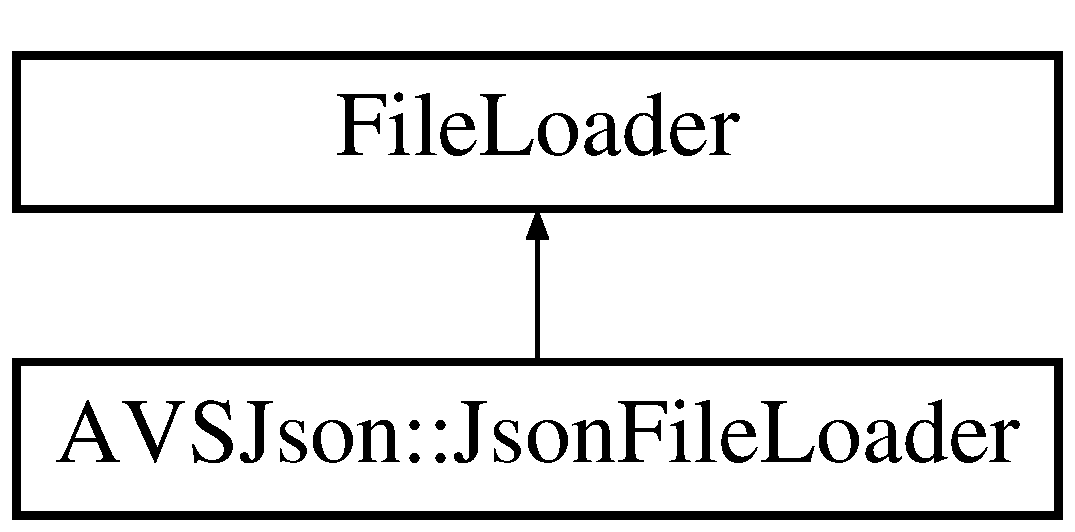
\includegraphics[height=2.000000cm]{d4/dbe/classAVSJson_1_1JsonFileLoader}
\end{center}
\end{figure}
\subsection*{Public Member Functions}
\begin{DoxyCompactItemize}
\item 
\mbox{\Hypertarget{classAVSJson_1_1JsonFileLoader_a7edbb0f861213e85bc835ee4bbd9e2df}\label{classAVSJson_1_1JsonFileLoader_a7edbb0f861213e85bc835ee4bbd9e2df}} 
{\bfseries Json\+File\+Loader} (const std\+::string json\+\_\+file\+\_\+name)
\item 
\mbox{\Hypertarget{classAVSJson_1_1JsonFileLoader_a864a274a345d6f1a16973e6abfedad76}\label{classAVSJson_1_1JsonFileLoader_a864a274a345d6f1a16973e6abfedad76}} 
void {\bfseries set\+Hashmap} (Json\+Hash\+Map map)
\item 
\mbox{\Hypertarget{classAVSJson_1_1JsonFileLoader_a05e6ad6b705addf961268179811f8976}\label{classAVSJson_1_1JsonFileLoader_a05e6ad6b705addf961268179811f8976}} 
void {\bfseries add\+Replace\+Data} (std\+::string search, std\+::string replace)
\item 
\mbox{\Hypertarget{classAVSJson_1_1JsonFileLoader_aa97f567ba6e9c358cc361109b5d23e72}\label{classAVSJson_1_1JsonFileLoader_aa97f567ba6e9c358cc361109b5d23e72}} 
const std\+::string {\bfseries get\+Json\+Object} (void)
\end{DoxyCompactItemize}
\subsection*{Protected Member Functions}
\begin{DoxyCompactItemize}
\item 
\mbox{\Hypertarget{classAVSJson_1_1JsonFileLoader_a39ca49e1e9168bc54564a90ff81cb562}\label{classAVSJson_1_1JsonFileLoader_a39ca49e1e9168bc54564a90ff81cb562}} 
void {\bfseries on\+Line\+Event} (const string line)
\item 
\mbox{\Hypertarget{classAVSJson_1_1JsonFileLoader_a7562ccc54984ea688e13b5fce560126c}\label{classAVSJson_1_1JsonFileLoader_a7562ccc54984ea688e13b5fce560126c}} 
void {\bfseries on\+End\+Of\+File\+Event} ()
\end{DoxyCompactItemize}


The documentation for this class was generated from the following files\+:\begin{DoxyCompactItemize}
\item 
/home/mutzi/progs/linux\+\_\+workspace/alexa-\/avs-\/prototype/src/include/jsonfileloader.\+h\item 
/home/mutzi/progs/linux\+\_\+workspace/alexa-\/avs-\/prototype/src/jsonfileloader.\+cpp\end{DoxyCompactItemize}

\hypertarget{structNetwork_1_1HTTP_1_1JsonObject}{}\section{Network\+:\+:H\+T\+TP\+:\+:Json\+Object Struct Reference}
\label{structNetwork_1_1HTTP_1_1JsonObject}\index{Network\+::\+H\+T\+T\+P\+::\+Json\+Object@{Network\+::\+H\+T\+T\+P\+::\+Json\+Object}}
\subsection*{Public Attributes}
\begin{DoxyCompactItemize}
\item 
\mbox{\Hypertarget{structNetwork_1_1HTTP_1_1JsonObject_ac377a85a255b170a019a49dc268a2934}\label{structNetwork_1_1HTTP_1_1JsonObject_ac377a85a255b170a019a49dc268a2934}} 
char $\ast$ {\bfseries json\+\_\+string}
\item 
\mbox{\Hypertarget{structNetwork_1_1HTTP_1_1JsonObject_a6c2fc1e835e83477ea06ae78dd1d83c9}\label{structNetwork_1_1HTTP_1_1JsonObject_a6c2fc1e835e83477ea06ae78dd1d83c9}} 
size\+\_\+t {\bfseries size}
\end{DoxyCompactItemize}


The documentation for this struct was generated from the following file\+:\begin{DoxyCompactItemize}
\item 
/home/mutzi/progs/linux\+\_\+workspace/alexa-\/avs-\/prototype/src/include/httpclientdirectiveevent.\+h\end{DoxyCompactItemize}

\hypertarget{classAVSJson_1_1JsonReaderDirective}{}\section{A\+V\+S\+Json\+:\+:Json\+Reader\+Directive Class Reference}
\label{classAVSJson_1_1JsonReaderDirective}\index{A\+V\+S\+Json\+::\+Json\+Reader\+Directive@{A\+V\+S\+Json\+::\+Json\+Reader\+Directive}}
\subsection*{Public Member Functions}
\begin{DoxyCompactItemize}
\item 
\mbox{\Hypertarget{classAVSJson_1_1JsonReaderDirective_ab6c68ee0fc053c88d3dfaa14c2244aee}\label{classAVSJson_1_1JsonReaderDirective_ab6c68ee0fc053c88d3dfaa14c2244aee}} 
{\bfseries Json\+Reader\+Directive} (const char $\ast$content)
\item 
\mbox{\Hypertarget{classAVSJson_1_1JsonReaderDirective_ad511f1ba5d09b960ef3f7dbc1fea675a}\label{classAVSJson_1_1JsonReaderDirective_ad511f1ba5d09b960ef3f7dbc1fea675a}} 
{\bfseries Json\+Reader\+Directive} (const std\+::string json\+\_\+content)
\item 
\mbox{\Hypertarget{classAVSJson_1_1JsonReaderDirective_a9b54950c28c51b173cbe089b64132ed2}\label{classAVSJson_1_1JsonReaderDirective_a9b54950c28c51b173cbe089b64132ed2}} 
void {\bfseries set\+Json\+Content} (const std\+::string json\+\_\+content)
\item 
\mbox{\Hypertarget{classAVSJson_1_1JsonReaderDirective_a6b11c4fde5d9317cd08921d533f3bf23}\label{classAVSJson_1_1JsonReaderDirective_a6b11c4fde5d9317cd08921d533f3bf23}} 
const std\+::string {\bfseries get\+Header\+Name\+Space} (void) const  throw ( std\+::exception )
\item 
\mbox{\Hypertarget{classAVSJson_1_1JsonReaderDirective_a62db5edd8cbefbafa5baefd0b1a8c42c}\label{classAVSJson_1_1JsonReaderDirective_a62db5edd8cbefbafa5baefd0b1a8c42c}} 
const std\+::string {\bfseries get\+Header\+Name} (void) const  throw ( std\+::exception )
\item 
\mbox{\Hypertarget{classAVSJson_1_1JsonReaderDirective_abf9ccee441e6bc2e76717a24ed93b5be}\label{classAVSJson_1_1JsonReaderDirective_abf9ccee441e6bc2e76717a24ed93b5be}} 
const std\+::string {\bfseries get\+Header\+Message\+Id} (void) const  throw ( std\+::exception )
\item 
\mbox{\Hypertarget{classAVSJson_1_1JsonReaderDirective_a5b591a4d16a05976e81f945752b3987b}\label{classAVSJson_1_1JsonReaderDirective_a5b591a4d16a05976e81f945752b3987b}} 
const std\+::string {\bfseries get\+Header\+Dialog\+Request\+Id} (void) const  throw ( std\+::exception )
\item 
\mbox{\Hypertarget{classAVSJson_1_1JsonReaderDirective_a3a39f22e2e80accfd1e556e3ce1083ee}\label{classAVSJson_1_1JsonReaderDirective_a3a39f22e2e80accfd1e556e3ce1083ee}} 
const std\+::string {\bfseries get\+Payload\+Url} (void) const  throw ( std\+::exception )
\item 
\mbox{\Hypertarget{classAVSJson_1_1JsonReaderDirective_a1ce0bd1b138273a93ebf40a549f99ed8}\label{classAVSJson_1_1JsonReaderDirective_a1ce0bd1b138273a93ebf40a549f99ed8}} 
const std\+::string {\bfseries get\+Payload\+Format} (void) const  throw ( std\+::exception )
\item 
\mbox{\Hypertarget{classAVSJson_1_1JsonReaderDirective_a6e79b09ca1bb989162d1129b83e29df5}\label{classAVSJson_1_1JsonReaderDirective_a6e79b09ca1bb989162d1129b83e29df5}} 
const std\+::string {\bfseries get\+Payload\+Token} (void) const  throw ( std\+::exception )
\item 
\mbox{\Hypertarget{classAVSJson_1_1JsonReaderDirective_a2b4054afd8feba7b1c6be7011f72a9ce}\label{classAVSJson_1_1JsonReaderDirective_a2b4054afd8feba7b1c6be7011f72a9ce}} 
const std\+::string {\bfseries get\+Payload\+Mute} (void) const  throw ( std\+::exception )
\end{DoxyCompactItemize}


The documentation for this class was generated from the following files\+:\begin{DoxyCompactItemize}
\item 
/home/mutzi/progs/linux\+\_\+workspace/alexa-\/avs-\/prototype/src/include/jsonreaderdirective.\+h\item 
/home/mutzi/progs/linux\+\_\+workspace/alexa-\/avs-\/prototype/src/jsonreader.\+cpp\end{DoxyCompactItemize}

\hypertarget{structstd_1_1less_3_1_1nlohmann_1_1detail_1_1value__t_01_4}{}\section{std\+:\+:less$<$\+:\+:nlohmann\+:\+:detail\+:\+:value\+\_\+t $>$ Struct Template Reference}
\label{structstd_1_1less_3_1_1nlohmann_1_1detail_1_1value__t_01_4}\index{std\+::less$<$\+::nlohmann\+::detail\+::value\+\_\+t $>$@{std\+::less$<$\+::nlohmann\+::detail\+::value\+\_\+t $>$}}


specialization for std\+::less$<$value\+\_\+t$>$  




{\ttfamily \#include $<$nlohmann\+\_\+json.\+h$>$}

\subsection*{Public Member Functions}
\begin{DoxyCompactItemize}
\item 
bool \hyperlink{structstd_1_1less_3_1_1nlohmann_1_1detail_1_1value__t_01_4_a10d3fea50edf7b15ead8f4ceeb006000}{operator()} (\hyperlink{namespacenlohmann_1_1detail_a90aa5ef615aa8305e9ea20d8a947980f}{nlohmann\+::detail\+::value\+\_\+t} lhs, \hyperlink{namespacenlohmann_1_1detail_a90aa5ef615aa8305e9ea20d8a947980f}{nlohmann\+::detail\+::value\+\_\+t} rhs) const noexcept
\begin{DoxyCompactList}\small\item\em compare two value\+\_\+t enum values \end{DoxyCompactList}\end{DoxyCompactItemize}


\subsection{Detailed Description}
\subsubsection*{template$<$$>$\newline
struct std\+::less$<$\+::nlohmann\+::detail\+::value\+\_\+t $>$}

specialization for std\+::less$<$value\+\_\+t$>$ 

\subsection{Member Function Documentation}
\mbox{\Hypertarget{structstd_1_1less_3_1_1nlohmann_1_1detail_1_1value__t_01_4_a10d3fea50edf7b15ead8f4ceeb006000}\label{structstd_1_1less_3_1_1nlohmann_1_1detail_1_1value__t_01_4_a10d3fea50edf7b15ead8f4ceeb006000}} 
\index{std\+::less$<$\+::nlohmann\+::detail\+::value\+\_\+t $>$@{std\+::less$<$\+::nlohmann\+::detail\+::value\+\_\+t $>$}!operator()@{operator()}}
\index{operator()@{operator()}!std\+::less$<$\+::nlohmann\+::detail\+::value\+\_\+t $>$@{std\+::less$<$\+::nlohmann\+::detail\+::value\+\_\+t $>$}}
\subsubsection{\texorpdfstring{operator()()}{operator()()}}
{\footnotesize\ttfamily bool std\+::less$<$\+::\hyperlink{namespacenlohmann_1_1detail_a90aa5ef615aa8305e9ea20d8a947980f}{nlohmann\+::detail\+::value\+\_\+t} $>$\+::operator() (\begin{DoxyParamCaption}\item[{\hyperlink{namespacenlohmann_1_1detail_a90aa5ef615aa8305e9ea20d8a947980f}{nlohmann\+::detail\+::value\+\_\+t}}]{lhs,  }\item[{\hyperlink{namespacenlohmann_1_1detail_a90aa5ef615aa8305e9ea20d8a947980f}{nlohmann\+::detail\+::value\+\_\+t}}]{rhs }\end{DoxyParamCaption}) const\hspace{0.3cm}{\ttfamily [inline]}, {\ttfamily [noexcept]}}



compare two value\+\_\+t enum values 

\begin{DoxySince}{Since}
version 3.\+0.\+0 
\end{DoxySince}


The documentation for this struct was generated from the following file\+:\begin{DoxyCompactItemize}
\item 
/home/mutzi/progs/linux\+\_\+workspace/alexa-\/avs-\/prototype/src/include/nlohmann\+\_\+json.\+h\end{DoxyCompactItemize}

\hypertarget{classLogger}{}\section{Logger Class Reference}
\label{classLogger}\index{Logger@{Logger}}
\subsection*{Classes}
\begin{DoxyCompactItemize}
\item 
class \hyperlink{classLogger_1_1Cleanup}{Cleanup}
\end{DoxyCompactItemize}
\subsection*{Public Member Functions}
\begin{DoxyCompactItemize}
\item 
\mbox{\Hypertarget{classLogger_a2e4b4c867ecfe260bc1f4d218806810c}\label{classLogger_a2e4b4c867ecfe260bc1f4d218806810c}} 
void {\bfseries log} (const std\+::string \&in\+Log\+Level, const std\+::string \&in\+Message)
\item 
\mbox{\Hypertarget{classLogger_a5cde5c21cb6934b132eaf8261b53e402}\label{classLogger_a5cde5c21cb6934b132eaf8261b53e402}} 
void {\bfseries info} (const std\+::string \&in\+Message)
\item 
\mbox{\Hypertarget{classLogger_a7cc462a7598d311aa4f2ec4fe518b93f}\label{classLogger_a7cc462a7598d311aa4f2ec4fe518b93f}} 
void {\bfseries info} (const std\+::string \&in\+Message, const std\+::string \&extend\+Message)
\item 
\mbox{\Hypertarget{classLogger_ac4e95734a63d169fcef24210f559693a}\label{classLogger_ac4e95734a63d169fcef24210f559693a}} 
void {\bfseries info} (const std\+::string \&in\+Message, int integer)
\item 
\mbox{\Hypertarget{classLogger_ad1933a0621041f405973dded2410cbc0}\label{classLogger_ad1933a0621041f405973dded2410cbc0}} 
void {\bfseries warn} (const std\+::string \&in\+Message)
\item 
\mbox{\Hypertarget{classLogger_ae533d83005cf0a3d7f51a16840fc018a}\label{classLogger_ae533d83005cf0a3d7f51a16840fc018a}} 
void {\bfseries warn} (\hyperlink{structErrorException}{Error\+Exception} e)
\item 
\mbox{\Hypertarget{classLogger_aeb984c2ca90a8aca582e647b249733e7}\label{classLogger_aeb984c2ca90a8aca582e647b249733e7}} 
void {\bfseries warn} (const std\+::string \&in\+Message, \hyperlink{structErrorException}{Error\+Exception} e)
\item 
\mbox{\Hypertarget{classLogger_a32a06234fc70ea5fb75f32b26cea4483}\label{classLogger_a32a06234fc70ea5fb75f32b26cea4483}} 
void {\bfseries debug} (const std\+::string \&in\+Message)
\item 
\mbox{\Hypertarget{classLogger_a0cd03a1667644704c93c30c52176a87c}\label{classLogger_a0cd03a1667644704c93c30c52176a87c}} 
void {\bfseries error} (const std\+::string \&in\+Message)
\item 
\mbox{\Hypertarget{classLogger_a0e554d398ab4ed57a651dceca352ddd3}\label{classLogger_a0e554d398ab4ed57a651dceca352ddd3}} 
void {\bfseries error} (\hyperlink{structErrorException}{Error\+Exception} e)
\item 
\mbox{\Hypertarget{classLogger_a6f80f9061863ffe36007bc661e6d9f45}\label{classLogger_a6f80f9061863ffe36007bc661e6d9f45}} 
void {\bfseries error} (const std\+::string \&in\+Message, \hyperlink{structErrorException}{Error\+Exception} e)
\end{DoxyCompactItemize}
\subsection*{Static Public Member Functions}
\begin{DoxyCompactItemize}
\item 
\mbox{\Hypertarget{classLogger_a4aa4d7c3b98f6e12e7ea8253da5ea0cd}\label{classLogger_a4aa4d7c3b98f6e12e7ea8253da5ea0cd}} 
static \hyperlink{classLogger}{Logger} \& {\bfseries instance} ()
\item 
\mbox{\Hypertarget{classLogger_a192b4230e191b7f6d38c50d8d20d3c9d}\label{classLogger_a192b4230e191b7f6d38c50d8d20d3c9d}} 
static \hyperlink{classLogger}{Logger} \& {\bfseries instance} (const std\+::string \&class\+\_\+name)
\end{DoxyCompactItemize}
\subsection*{Static Public Attributes}
\begin{DoxyCompactItemize}
\item 
\mbox{\Hypertarget{classLogger_a13508ec720a1c2f885793ea84befc58e}\label{classLogger_a13508ec720a1c2f885793ea84befc58e}} 
static const std\+::string {\bfseries k\+Log\+Level\+Debug} = \char`\"{}D\+E\+B\+UG\char`\"{}
\item 
\mbox{\Hypertarget{classLogger_a8e72302e1254e7f840cfc1cbd9cbd615}\label{classLogger_a8e72302e1254e7f840cfc1cbd9cbd615}} 
static const std\+::string {\bfseries k\+Log\+Level\+Info} = \char`\"{}I\+N\+FO\char`\"{}
\item 
\mbox{\Hypertarget{classLogger_a8e4174e48cfc36ad766e26d0a16cd5cd}\label{classLogger_a8e4174e48cfc36ad766e26d0a16cd5cd}} 
static const std\+::string {\bfseries k\+Log\+Level\+Warning} = \char`\"{}W\+A\+R\+N\+I\+NG\char`\"{}
\item 
\mbox{\Hypertarget{classLogger_a848ce96cde882ab0709ee26bbd22a5cf}\label{classLogger_a848ce96cde882ab0709ee26bbd22a5cf}} 
static const std\+::string {\bfseries k\+Log\+Level\+Error} = \char`\"{}E\+R\+R\+OR\char`\"{}
\end{DoxyCompactItemize}
\subsection*{Protected Member Functions}
\begin{DoxyCompactItemize}
\item 
\mbox{\Hypertarget{classLogger_a95312ad188bc0ffaae6e81e7232fea56}\label{classLogger_a95312ad188bc0ffaae6e81e7232fea56}} 
void {\bfseries log\+Helper} (const std\+::string \&in\+Log\+Level, const std\+::string \&in\+Message)
\end{DoxyCompactItemize}
\subsection*{Protected Attributes}
\begin{DoxyCompactItemize}
\item 
\mbox{\Hypertarget{classLogger_a9cba5476c807435980221f095ba336ad}\label{classLogger_a9cba5476c807435980221f095ba336ad}} 
std\+::ofstream {\bfseries m\+\_\+output\+\_\+stream}
\end{DoxyCompactItemize}
\subsection*{Static Protected Attributes}
\begin{DoxyCompactItemize}
\item 
\mbox{\Hypertarget{classLogger_aa2b461b4d0dc897500899b57cc446ead}\label{classLogger_aa2b461b4d0dc897500899b57cc446ead}} 
static \hyperlink{classLogger}{Logger} $\ast$ {\bfseries p\+Instance} = nullptr
\item 
\mbox{\Hypertarget{classLogger_a5d70bcbb122d00ecc958df45439b96f3}\label{classLogger_a5d70bcbb122d00ecc958df45439b96f3}} 
static const char $\ast$const {\bfseries k\+Log\+File\+Name} = \char`\"{}application.\+log\char`\"{}
\end{DoxyCompactItemize}
\subsection*{Friends}
\begin{DoxyCompactItemize}
\item 
\mbox{\Hypertarget{classLogger_ac3dfceef1470d020a70636b08149121a}\label{classLogger_ac3dfceef1470d020a70636b08149121a}} 
class {\bfseries Cleanup}
\end{DoxyCompactItemize}


The documentation for this class was generated from the following files\+:\begin{DoxyCompactItemize}
\item 
/home/mutzi/progs/linux\+\_\+workspace/alexa-\/avs-\/prototype/src/include/logger.\+h\item 
/home/mutzi/progs/linux\+\_\+workspace/alexa-\/avs-\/prototype/src/logger.\+cpp\end{DoxyCompactItemize}

\hypertarget{structnlohmann_1_1detail_1_1negation}{}\section{nlohmann\+:\+:detail\+:\+:negation$<$ B $>$ Struct Template Reference}
\label{structnlohmann_1_1detail_1_1negation}\index{nlohmann\+::detail\+::negation$<$ B $>$@{nlohmann\+::detail\+::negation$<$ B $>$}}
Inheritance diagram for nlohmann\+:\+:detail\+:\+:negation$<$ B $>$\+:\begin{figure}[H]
\begin{center}
\leavevmode
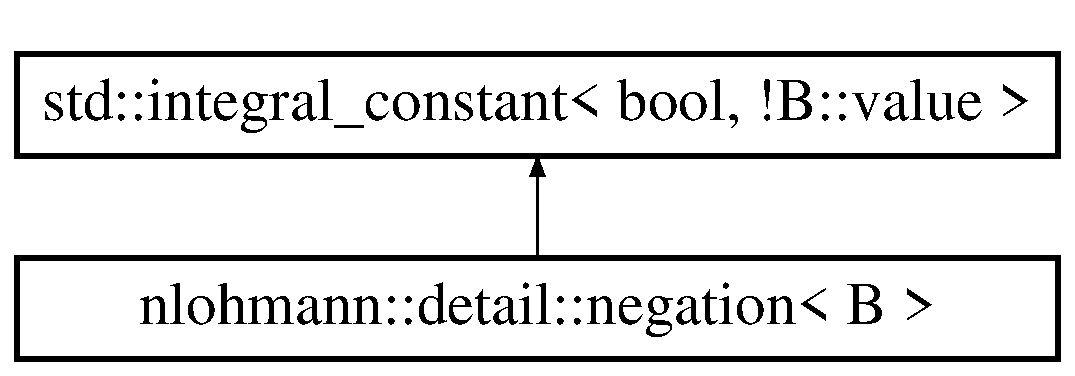
\includegraphics[height=2.000000cm]{d1/d91/structnlohmann_1_1detail_1_1negation}
\end{center}
\end{figure}


The documentation for this struct was generated from the following file\+:\begin{DoxyCompactItemize}
\item 
/home/mutzi/progs/linux\+\_\+workspace/alexa-\/avs-\/prototype/src/include/nlohmann\+\_\+json.\+h\end{DoxyCompactItemize}

\hypertarget{classNetwork_1_1HTTP2_1_1NgHTTP2API}{}\section{Network\+:\+:H\+T\+T\+P2\+:\+:Ng\+H\+T\+T\+P2\+A\+PI Class Reference}
\label{classNetwork_1_1HTTP2_1_1NgHTTP2API}\index{Network\+::\+H\+T\+T\+P2\+::\+Ng\+H\+T\+T\+P2\+A\+PI@{Network\+::\+H\+T\+T\+P2\+::\+Ng\+H\+T\+T\+P2\+A\+PI}}
Inheritance diagram for Network\+:\+:H\+T\+T\+P2\+:\+:Ng\+H\+T\+T\+P2\+A\+PI\+:\begin{figure}[H]
\begin{center}
\leavevmode
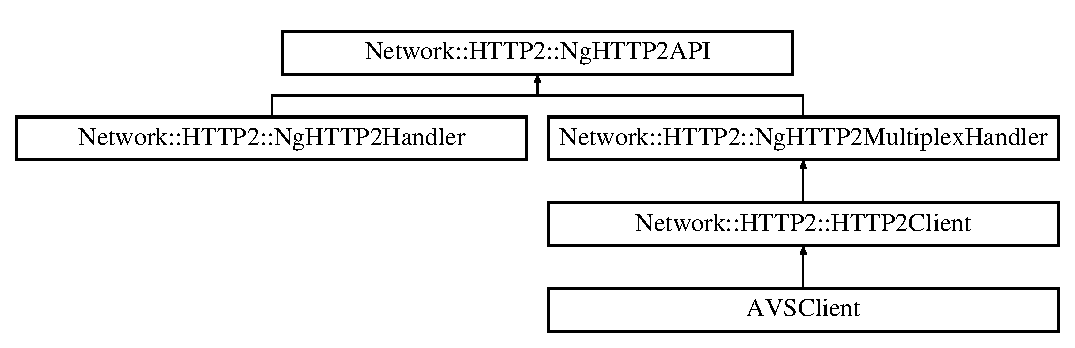
\includegraphics[height=4.000000cm]{dc/db7/classNetwork_1_1HTTP2_1_1NgHTTP2API}
\end{center}
\end{figure}
\subsection*{Public Member Functions}
\begin{DoxyCompactItemize}
\item 
void \hyperlink{classNetwork_1_1HTTP2_1_1NgHTTP2API_a83048a73d75bda59e9f6b1c97039468e}{set\+Read\+Callback} (H\+T\+T\+P2\+Response\+Header\+Callback header, H\+T\+T\+P2\+Response\+Body\+Callback body, void $\ast$user\+\_\+data)
\begin{DoxyCompactList}\small\item\em set\+Read\+Callback \end{DoxyCompactList}\item 
S\+S\+L\+\_\+\+C\+TX $\ast$ \hyperlink{classNetwork_1_1HTTP2_1_1NgHTTP2API_ac6e30f8c88ca773da99ce34724a7dfd0}{create\+\_\+ssl\+\_\+ctx} (void)
\begin{DoxyCompactList}\small\item\em create\+\_\+ssl\+\_\+ctx \end{DoxyCompactList}\item 
void \hyperlink{classNetwork_1_1HTTP2_1_1NgHTTP2API_aaff2b630490f8d10c845996f927fd4d8}{initiate\+\_\+connection} (struct event\+\_\+base $\ast$evbase, S\+S\+L\+\_\+\+C\+TX $\ast$ssl\+\_\+ctx, const char $\ast$host, uint16\+\_\+t port, \hyperlink{structNetwork_1_1HTTP2_1_1http2__session__data}{http2\+\_\+session\+\_\+data} $\ast$session\+\_\+data)
\begin{DoxyCompactList}\small\item\em initiate\+\_\+connection \end{DoxyCompactList}\item 
\hyperlink{structNetwork_1_1HTTP2_1_1http2__session__data}{http2\+\_\+session\+\_\+data} $\ast$ \hyperlink{classNetwork_1_1HTTP2_1_1NgHTTP2API_a83fa51a83722d8aeab16465c937cc41f}{create\+\_\+http2\+\_\+session\+\_\+data} (struct evdns\+\_\+base $\ast$dnsbase, \hyperlink{classNetwork_1_1HTTP2_1_1NgHTTP2API}{Ng\+H\+T\+T\+P2\+A\+PI} $\ast$api)
\begin{DoxyCompactList}\small\item\em create\+\_\+http2\+\_\+session\+\_\+data \end{DoxyCompactList}\item 
\mbox{\Hypertarget{classNetwork_1_1HTTP2_1_1NgHTTP2API_a1ba3edf107165568b6a0b4138b285ed9}\label{classNetwork_1_1HTTP2_1_1NgHTTP2API_a1ba3edf107165568b6a0b4138b285ed9}} 
\hyperlink{structNetwork_1_1HTTP2_1_1http2__session__data}{http2\+\_\+session\+\_\+data} $\ast$ {\bfseries create\+\_\+http2\+\_\+connection\+\_\+session\+\_\+data} (struct event\+\_\+base $\ast$evbase, \hyperlink{classNetwork_1_1HTTP2_1_1NgHTTP2API}{Ng\+H\+T\+T\+P2\+A\+PI} $\ast$api)
\end{DoxyCompactItemize}
\subsection*{Static Protected Member Functions}
\begin{DoxyCompactItemize}
\item 
static int \hyperlink{classNetwork_1_1HTTP2_1_1NgHTTP2API_af03f36272bba30d171567765cde46c86}{select\+\_\+next\+\_\+proto\+\_\+cb} (S\+SL $\ast$ssl, unsigned char $\ast$$\ast$out, unsigned char $\ast$outlen, const unsigned char $\ast$in, unsigned int inlen, void $\ast$arg)
\begin{DoxyCompactList}\small\item\em select\+\_\+next\+\_\+proto\+\_\+cb \+: callback function \end{DoxyCompactList}\item 
static S\+SL $\ast$ \hyperlink{classNetwork_1_1HTTP2_1_1NgHTTP2API_a3dba39aa33a1c629359d76a66d92ec0d}{create\+\_\+ssl} (S\+S\+L\+\_\+\+C\+TX $\ast$ssl\+\_\+ctx)
\begin{DoxyCompactList}\small\item\em create\+\_\+ssl \end{DoxyCompactList}\item 
static void \hyperlink{classNetwork_1_1HTTP2_1_1NgHTTP2API_a0356d7de7d3df4fa59b91610dcbaf5ef}{eventcb} (struct bufferevent $\ast$bev, short events, void $\ast$ptr)
\begin{DoxyCompactList}\small\item\em eventcb \+: callback function \end{DoxyCompactList}\item 
static void \hyperlink{classNetwork_1_1HTTP2_1_1NgHTTP2API_a9f3146f288f2fb033296b6e43564cc7b}{readcb} (struct bufferevent $\ast$bev, void $\ast$ptr)
\begin{DoxyCompactList}\small\item\em readcb \+: callback function \end{DoxyCompactList}\item 
static void \hyperlink{classNetwork_1_1HTTP2_1_1NgHTTP2API_a5d047441518239869e1c699323ee3c92}{writecb} (struct bufferevent $\ast$bev, void $\ast$ptr)
\begin{DoxyCompactList}\small\item\em writecb \+: callback function \end{DoxyCompactList}\item 
static void \hyperlink{classNetwork_1_1HTTP2_1_1NgHTTP2API_ac54322656bb0db60581bbcae17a18e1a}{initialize\+\_\+nghttp2\+\_\+session} (\hyperlink{structNetwork_1_1HTTP2_1_1http2__session__data}{http2\+\_\+session\+\_\+data} $\ast$session\+\_\+data)
\begin{DoxyCompactList}\small\item\em initialize\+\_\+nghttp2\+\_\+session \end{DoxyCompactList}\item 
static void \hyperlink{classNetwork_1_1HTTP2_1_1NgHTTP2API_aaf79d1a5a4e907ba727c8a5b8520c7ae}{send\+\_\+client\+\_\+connection\+\_\+header} (\hyperlink{structNetwork_1_1HTTP2_1_1http2__session__data}{http2\+\_\+session\+\_\+data} $\ast$session\+\_\+data)
\begin{DoxyCompactList}\small\item\em send\+\_\+client\+\_\+connection\+\_\+header \end{DoxyCompactList}\item 
static void \hyperlink{classNetwork_1_1HTTP2_1_1NgHTTP2API_a27e408f85d4199cd26250c59ba13553f}{submit\+\_\+request} (\hyperlink{structNetwork_1_1HTTP2_1_1http2__session__data}{http2\+\_\+session\+\_\+data} $\ast$session\+\_\+data)
\item 
static void \hyperlink{classNetwork_1_1HTTP2_1_1NgHTTP2API_a6ed7953f91c559adef118fbfa7e96d46}{submit\+\_\+data} (\hyperlink{structNetwork_1_1HTTP2_1_1http2__session__data}{http2\+\_\+session\+\_\+data} $\ast$session\+\_\+data)
\begin{DoxyCompactList}\small\item\em submit\+\_\+data \end{DoxyCompactList}\item 
static int \hyperlink{classNetwork_1_1HTTP2_1_1NgHTTP2API_a98fcbd6599625a1fdaec14f49095bc7a}{session\+\_\+send} (\hyperlink{structNetwork_1_1HTTP2_1_1http2__session__data}{http2\+\_\+session\+\_\+data} $\ast$session\+\_\+data)
\begin{DoxyCompactList}\small\item\em session\+\_\+send \end{DoxyCompactList}\item 
static ssize\+\_\+t \hyperlink{classNetwork_1_1HTTP2_1_1NgHTTP2API_a419c427d7059d6d1858136f6913a1ae6}{data\+\_\+source\+\_\+read\+\_\+callback} (nghttp2\+\_\+session $\ast$session, int32\+\_\+t stream\+\_\+id, uint8\+\_\+t $\ast$buf, size\+\_\+t length, uint32\+\_\+t $\ast$data\+\_\+flags, nghttp2\+\_\+data\+\_\+source $\ast$source, void $\ast$user\+\_\+data)
\begin{DoxyCompactList}\small\item\em data\+\_\+source\+\_\+read\+\_\+callback \+: callback function \end{DoxyCompactList}\item 
static ssize\+\_\+t \hyperlink{classNetwork_1_1HTTP2_1_1NgHTTP2API_aef0ee4f04992e02b2aa2916e89e03114}{send\+\_\+callback} (nghttp2\+\_\+session $\ast$session, const uint8\+\_\+t $\ast$data, size\+\_\+t length, int flags, void $\ast$user\+\_\+data)
\begin{DoxyCompactList}\small\item\em send\+\_\+callback \+: callback function \end{DoxyCompactList}\item 
static int \hyperlink{classNetwork_1_1HTTP2_1_1NgHTTP2API_a64f69e8e4726d3baec216cfeb786e6fe}{on\+\_\+header\+\_\+callback} (nghttp2\+\_\+session $\ast$session, const nghttp2\+\_\+frame $\ast$frame, const uint8\+\_\+t $\ast$name, size\+\_\+t namelen, const uint8\+\_\+t $\ast$value, size\+\_\+t valuelen, uint8\+\_\+t flags, void $\ast$user\+\_\+data)
\begin{DoxyCompactList}\small\item\em on\+\_\+header\+\_\+callback \+: callback function \end{DoxyCompactList}\item 
static int \hyperlink{classNetwork_1_1HTTP2_1_1NgHTTP2API_adc5ac253870d245cee1ce1c890b7b4e6}{on\+\_\+frame\+\_\+recv\+\_\+callback} (nghttp2\+\_\+session $\ast$session, const nghttp2\+\_\+frame $\ast$frame, void $\ast$user\+\_\+data)
\begin{DoxyCompactList}\small\item\em on\+\_\+frame\+\_\+recv\+\_\+callback \+: callback function \end{DoxyCompactList}\item 
\mbox{\Hypertarget{classNetwork_1_1HTTP2_1_1NgHTTP2API_ae5528b49178920157febd62a8f1b8179}\label{classNetwork_1_1HTTP2_1_1NgHTTP2API_ae5528b49178920157febd62a8f1b8179}} 
static int {\bfseries on\+\_\+frame\+\_\+send\+\_\+callback} (nghttp2\+\_\+session $\ast$session, const nghttp2\+\_\+frame $\ast$fame, void $\ast$user\+\_\+data)
\item 
static int \hyperlink{classNetwork_1_1HTTP2_1_1NgHTTP2API_a479aebf9b74b978712a20a1db27ab164}{on\+\_\+data\+\_\+chunk\+\_\+recv\+\_\+callback} (nghttp2\+\_\+session $\ast$session, uint8\+\_\+t flags, int32\+\_\+t stream\+\_\+id, const uint8\+\_\+t $\ast$data, size\+\_\+t len, void $\ast$user\+\_\+data)
\begin{DoxyCompactList}\small\item\em on\+\_\+data\+\_\+chunk\+\_\+recv\+\_\+callback \+: callback function \end{DoxyCompactList}\item 
static int \hyperlink{classNetwork_1_1HTTP2_1_1NgHTTP2API_ad3e61d93b5d2381d4efccf96ac950ad1}{on\+\_\+stream\+\_\+close\+\_\+callback} (nghttp2\+\_\+session $\ast$session, int32\+\_\+t stream\+\_\+id, uint32\+\_\+t error\+\_\+code, void $\ast$user\+\_\+data)
\begin{DoxyCompactList}\small\item\em on\+\_\+stream\+\_\+close\+\_\+callback \end{DoxyCompactList}\item 
static int \hyperlink{classNetwork_1_1HTTP2_1_1NgHTTP2API_a5798eb1a4f55819d0a276be86fe706e9}{on\+\_\+begin\+\_\+headers\+\_\+callback} (nghttp2\+\_\+session $\ast$session, const nghttp2\+\_\+frame $\ast$frame, void $\ast$user\+\_\+data)
\begin{DoxyCompactList}\small\item\em on\+\_\+begin\+\_\+headers\+\_\+callback \+: callback function \end{DoxyCompactList}\item 
\mbox{\Hypertarget{classNetwork_1_1HTTP2_1_1NgHTTP2API_ab48a1a1b46569fb6ab3e2ecd948ff431}\label{classNetwork_1_1HTTP2_1_1NgHTTP2API_ab48a1a1b46569fb6ab3e2ecd948ff431}} 
static void {\bfseries delete\+\_\+http2\+\_\+session\+\_\+data} (\hyperlink{structNetwork_1_1HTTP2_1_1http2__session__data}{http2\+\_\+session\+\_\+data} $\ast$session\+\_\+data)
\item 
\mbox{\Hypertarget{classNetwork_1_1HTTP2_1_1NgHTTP2API_a8685e090e286b9a4168299a7d89ab2d4}\label{classNetwork_1_1HTTP2_1_1NgHTTP2API_a8685e090e286b9a4168299a7d89ab2d4}} 
static void {\bfseries print\+\_\+header} (F\+I\+LE $\ast$f, const uint8\+\_\+t $\ast$name, size\+\_\+t namelen, const uint8\+\_\+t $\ast$value, size\+\_\+t valuelen)
\item 
\mbox{\Hypertarget{classNetwork_1_1HTTP2_1_1NgHTTP2API_a291da48b0e209ed27c47f950b36b088a}\label{classNetwork_1_1HTTP2_1_1NgHTTP2API_a291da48b0e209ed27c47f950b36b088a}} 
static void {\bfseries print\+\_\+headers} (F\+I\+LE $\ast$f, nghttp2\+\_\+nv $\ast$nva, size\+\_\+t nvlen)
\end{DoxyCompactItemize}
\subsection*{Protected Attributes}
\begin{DoxyCompactItemize}
\item 
\mbox{\Hypertarget{classNetwork_1_1HTTP2_1_1NgHTTP2API_aafbb434466a988c7b364fd2359d5a273}\label{classNetwork_1_1HTTP2_1_1NgHTTP2API_aafbb434466a988c7b364fd2359d5a273}} 
H\+T\+T\+P2\+Response\+Header\+Callback {\bfseries m\+\_\+response\+\_\+header\+\_\+callback}
\item 
\mbox{\Hypertarget{classNetwork_1_1HTTP2_1_1NgHTTP2API_aff09e9e26af77859c94dcdd3d76f8472}\label{classNetwork_1_1HTTP2_1_1NgHTTP2API_aff09e9e26af77859c94dcdd3d76f8472}} 
H\+T\+T\+P2\+Response\+Body\+Callback {\bfseries m\+\_\+response\+\_\+body\+\_\+callback}
\item 
\mbox{\Hypertarget{classNetwork_1_1HTTP2_1_1NgHTTP2API_ad8c875a52bbdc2e93707698787998d8d}\label{classNetwork_1_1HTTP2_1_1NgHTTP2API_ad8c875a52bbdc2e93707698787998d8d}} 
void $\ast$ {\bfseries m\+\_\+response\+\_\+user\+\_\+data}
\end{DoxyCompactItemize}


\subsection{Member Function Documentation}
\mbox{\Hypertarget{classNetwork_1_1HTTP2_1_1NgHTTP2API_a83fa51a83722d8aeab16465c937cc41f}\label{classNetwork_1_1HTTP2_1_1NgHTTP2API_a83fa51a83722d8aeab16465c937cc41f}} 
\index{Network\+::\+H\+T\+T\+P2\+::\+Ng\+H\+T\+T\+P2\+A\+PI@{Network\+::\+H\+T\+T\+P2\+::\+Ng\+H\+T\+T\+P2\+A\+PI}!create\+\_\+http2\+\_\+session\+\_\+data@{create\+\_\+http2\+\_\+session\+\_\+data}}
\index{create\+\_\+http2\+\_\+session\+\_\+data@{create\+\_\+http2\+\_\+session\+\_\+data}!Network\+::\+H\+T\+T\+P2\+::\+Ng\+H\+T\+T\+P2\+A\+PI@{Network\+::\+H\+T\+T\+P2\+::\+Ng\+H\+T\+T\+P2\+A\+PI}}
\subsubsection{\texorpdfstring{create\+\_\+http2\+\_\+session\+\_\+data()}{create\_http2\_session\_data()}}
{\footnotesize\ttfamily \hyperlink{structNetwork_1_1HTTP2_1_1http2__session__data}{http2\+\_\+session\+\_\+data} $\ast$ Ng\+H\+T\+T\+P2\+A\+P\+I\+::create\+\_\+http2\+\_\+session\+\_\+data (\begin{DoxyParamCaption}\item[{struct evdns\+\_\+base $\ast$}]{dnsbase,  }\item[{\hyperlink{classNetwork_1_1HTTP2_1_1NgHTTP2API}{Ng\+H\+T\+T\+P2\+A\+PI} $\ast$}]{api }\end{DoxyParamCaption})}



create\+\_\+http2\+\_\+session\+\_\+data 

Create H\+T\+T\+P2 Session 
\begin{DoxyParams}{Parameters}
{\em evbase} & \\
\hline
\end{DoxyParams}
\begin{DoxyReturn}{Returns}

\end{DoxyReturn}
\mbox{\Hypertarget{classNetwork_1_1HTTP2_1_1NgHTTP2API_a3dba39aa33a1c629359d76a66d92ec0d}\label{classNetwork_1_1HTTP2_1_1NgHTTP2API_a3dba39aa33a1c629359d76a66d92ec0d}} 
\index{Network\+::\+H\+T\+T\+P2\+::\+Ng\+H\+T\+T\+P2\+A\+PI@{Network\+::\+H\+T\+T\+P2\+::\+Ng\+H\+T\+T\+P2\+A\+PI}!create\+\_\+ssl@{create\+\_\+ssl}}
\index{create\+\_\+ssl@{create\+\_\+ssl}!Network\+::\+H\+T\+T\+P2\+::\+Ng\+H\+T\+T\+P2\+A\+PI@{Network\+::\+H\+T\+T\+P2\+::\+Ng\+H\+T\+T\+P2\+A\+PI}}
\subsubsection{\texorpdfstring{create\+\_\+ssl()}{create\_ssl()}}
{\footnotesize\ttfamily S\+SL $\ast$ Ng\+H\+T\+T\+P2\+A\+P\+I\+::create\+\_\+ssl (\begin{DoxyParamCaption}\item[{S\+S\+L\+\_\+\+C\+TX $\ast$}]{ssl\+\_\+ctx }\end{DoxyParamCaption})\hspace{0.3cm}{\ttfamily [static]}, {\ttfamily [protected]}}



create\+\_\+ssl 

Create S\+SL function Invoke from \+: \hyperlink{classNetwork_1_1HTTP2_1_1NgHTTP2API_aaff2b630490f8d10c845996f927fd4d8}{Ng\+H\+T\+T\+P2\+A\+P\+I\+::initiate\+\_\+connection} 
\begin{DoxyParams}{Parameters}
{\em ssl\+\_\+ctx} & \\
\hline
\end{DoxyParams}
\begin{DoxyReturn}{Returns}

\end{DoxyReturn}
\mbox{\Hypertarget{classNetwork_1_1HTTP2_1_1NgHTTP2API_ac6e30f8c88ca773da99ce34724a7dfd0}\label{classNetwork_1_1HTTP2_1_1NgHTTP2API_ac6e30f8c88ca773da99ce34724a7dfd0}} 
\index{Network\+::\+H\+T\+T\+P2\+::\+Ng\+H\+T\+T\+P2\+A\+PI@{Network\+::\+H\+T\+T\+P2\+::\+Ng\+H\+T\+T\+P2\+A\+PI}!create\+\_\+ssl\+\_\+ctx@{create\+\_\+ssl\+\_\+ctx}}
\index{create\+\_\+ssl\+\_\+ctx@{create\+\_\+ssl\+\_\+ctx}!Network\+::\+H\+T\+T\+P2\+::\+Ng\+H\+T\+T\+P2\+A\+PI@{Network\+::\+H\+T\+T\+P2\+::\+Ng\+H\+T\+T\+P2\+A\+PI}}
\subsubsection{\texorpdfstring{create\+\_\+ssl\+\_\+ctx()}{create\_ssl\_ctx()}}
{\footnotesize\ttfamily S\+S\+L\+\_\+\+C\+TX $\ast$ Ng\+H\+T\+T\+P2\+A\+P\+I\+::create\+\_\+ssl\+\_\+ctx (\begin{DoxyParamCaption}\item[{void}]{ }\end{DoxyParamCaption})}



create\+\_\+ssl\+\_\+ctx 

Create S\+SL C\+TX \begin{DoxyReturn}{Returns}

\end{DoxyReturn}
\mbox{\Hypertarget{classNetwork_1_1HTTP2_1_1NgHTTP2API_a419c427d7059d6d1858136f6913a1ae6}\label{classNetwork_1_1HTTP2_1_1NgHTTP2API_a419c427d7059d6d1858136f6913a1ae6}} 
\index{Network\+::\+H\+T\+T\+P2\+::\+Ng\+H\+T\+T\+P2\+A\+PI@{Network\+::\+H\+T\+T\+P2\+::\+Ng\+H\+T\+T\+P2\+A\+PI}!data\+\_\+source\+\_\+read\+\_\+callback@{data\+\_\+source\+\_\+read\+\_\+callback}}
\index{data\+\_\+source\+\_\+read\+\_\+callback@{data\+\_\+source\+\_\+read\+\_\+callback}!Network\+::\+H\+T\+T\+P2\+::\+Ng\+H\+T\+T\+P2\+A\+PI@{Network\+::\+H\+T\+T\+P2\+::\+Ng\+H\+T\+T\+P2\+A\+PI}}
\subsubsection{\texorpdfstring{data\+\_\+source\+\_\+read\+\_\+callback()}{data\_source\_read\_callback()}}
{\footnotesize\ttfamily ssize\+\_\+t Ng\+H\+T\+T\+P2\+A\+P\+I\+::data\+\_\+source\+\_\+read\+\_\+callback (\begin{DoxyParamCaption}\item[{nghttp2\+\_\+session $\ast$}]{session,  }\item[{int32\+\_\+t}]{stream\+\_\+id,  }\item[{uint8\+\_\+t $\ast$}]{buf,  }\item[{size\+\_\+t}]{length,  }\item[{uint32\+\_\+t $\ast$}]{data\+\_\+flags,  }\item[{nghttp2\+\_\+data\+\_\+source $\ast$}]{source,  }\item[{void $\ast$}]{user\+\_\+data }\end{DoxyParamCaption})\hspace{0.3cm}{\ttfamily [static]}, {\ttfamily [protected]}}



data\+\_\+source\+\_\+read\+\_\+callback \+: callback function 

Read Data Source ( Body Request )


\begin{DoxyParams}{Parameters}
{\em session} & \\
\hline
{\em stream\+\_\+id} & \\
\hline
{\em buf} & \\
\hline
{\em length} & \\
\hline
{\em data\+\_\+flags} & \\
\hline
{\em source} & \\
\hline
{\em user\+\_\+data} & \+: \hyperlink{structNetwork_1_1HTTP2_1_1http2__session__data}{http2\+\_\+session\+\_\+data} \\
\hline
\end{DoxyParams}
\begin{DoxyReturn}{Returns}

\end{DoxyReturn}
\mbox{\Hypertarget{classNetwork_1_1HTTP2_1_1NgHTTP2API_a0356d7de7d3df4fa59b91610dcbaf5ef}\label{classNetwork_1_1HTTP2_1_1NgHTTP2API_a0356d7de7d3df4fa59b91610dcbaf5ef}} 
\index{Network\+::\+H\+T\+T\+P2\+::\+Ng\+H\+T\+T\+P2\+A\+PI@{Network\+::\+H\+T\+T\+P2\+::\+Ng\+H\+T\+T\+P2\+A\+PI}!eventcb@{eventcb}}
\index{eventcb@{eventcb}!Network\+::\+H\+T\+T\+P2\+::\+Ng\+H\+T\+T\+P2\+A\+PI@{Network\+::\+H\+T\+T\+P2\+::\+Ng\+H\+T\+T\+P2\+A\+PI}}
\subsubsection{\texorpdfstring{eventcb()}{eventcb()}}
{\footnotesize\ttfamily void Ng\+H\+T\+T\+P2\+A\+P\+I\+::eventcb (\begin{DoxyParamCaption}\item[{struct bufferevent $\ast$}]{bev,  }\item[{short}]{events,  }\item[{void $\ast$}]{ptr }\end{DoxyParamCaption})\hspace{0.3cm}{\ttfamily [static]}, {\ttfamily [protected]}}



eventcb \+: callback function 

Buffer\+Event -\/ Managed Events

B\+E\+V\+\_\+\+E\+V\+E\+N\+T\+\_\+\+C\+O\+N\+N\+E\+C\+T\+ED B\+E\+V\+\_\+\+E\+V\+E\+N\+T\+\_\+\+E\+OF B\+E\+V\+\_\+\+E\+V\+E\+N\+T\+\_\+\+E\+R\+R\+OR B\+E\+V\+\_\+\+E\+V\+E\+N\+T\+\_\+\+T\+I\+M\+E\+O\+UT


\begin{DoxyParams}{Parameters}
{\em bev} & \\
\hline
{\em events} & \\
\hline
{\em ptr} & \+: http\+\_\+session\+\_\+data \\
\hline
\end{DoxyParams}
\mbox{\Hypertarget{classNetwork_1_1HTTP2_1_1NgHTTP2API_ac54322656bb0db60581bbcae17a18e1a}\label{classNetwork_1_1HTTP2_1_1NgHTTP2API_ac54322656bb0db60581bbcae17a18e1a}} 
\index{Network\+::\+H\+T\+T\+P2\+::\+Ng\+H\+T\+T\+P2\+A\+PI@{Network\+::\+H\+T\+T\+P2\+::\+Ng\+H\+T\+T\+P2\+A\+PI}!initialize\+\_\+nghttp2\+\_\+session@{initialize\+\_\+nghttp2\+\_\+session}}
\index{initialize\+\_\+nghttp2\+\_\+session@{initialize\+\_\+nghttp2\+\_\+session}!Network\+::\+H\+T\+T\+P2\+::\+Ng\+H\+T\+T\+P2\+A\+PI@{Network\+::\+H\+T\+T\+P2\+::\+Ng\+H\+T\+T\+P2\+A\+PI}}
\subsubsection{\texorpdfstring{initialize\+\_\+nghttp2\+\_\+session()}{initialize\_nghttp2\_session()}}
{\footnotesize\ttfamily void Ng\+H\+T\+T\+P2\+A\+P\+I\+::initialize\+\_\+nghttp2\+\_\+session (\begin{DoxyParamCaption}\item[{\hyperlink{structNetwork_1_1HTTP2_1_1http2__session__data}{http2\+\_\+session\+\_\+data} $\ast$}]{session\+\_\+data }\end{DoxyParamCaption})\hspace{0.3cm}{\ttfamily [static]}, {\ttfamily [protected]}}



initialize\+\_\+nghttp2\+\_\+session 

Create nghttp2\+\_\+session

and setup callbacks 
\begin{DoxyParams}{Parameters}
{\em session\+\_\+data} & \\
\hline
\end{DoxyParams}
\mbox{\Hypertarget{classNetwork_1_1HTTP2_1_1NgHTTP2API_aaff2b630490f8d10c845996f927fd4d8}\label{classNetwork_1_1HTTP2_1_1NgHTTP2API_aaff2b630490f8d10c845996f927fd4d8}} 
\index{Network\+::\+H\+T\+T\+P2\+::\+Ng\+H\+T\+T\+P2\+A\+PI@{Network\+::\+H\+T\+T\+P2\+::\+Ng\+H\+T\+T\+P2\+A\+PI}!initiate\+\_\+connection@{initiate\+\_\+connection}}
\index{initiate\+\_\+connection@{initiate\+\_\+connection}!Network\+::\+H\+T\+T\+P2\+::\+Ng\+H\+T\+T\+P2\+A\+PI@{Network\+::\+H\+T\+T\+P2\+::\+Ng\+H\+T\+T\+P2\+A\+PI}}
\subsubsection{\texorpdfstring{initiate\+\_\+connection()}{initiate\_connection()}}
{\footnotesize\ttfamily void Ng\+H\+T\+T\+P2\+A\+P\+I\+::initiate\+\_\+connection (\begin{DoxyParamCaption}\item[{struct event\+\_\+base $\ast$}]{evbase,  }\item[{S\+S\+L\+\_\+\+C\+TX $\ast$}]{ssl\+\_\+ctx,  }\item[{const char $\ast$}]{host,  }\item[{uint16\+\_\+t}]{port,  }\item[{\hyperlink{structNetwork_1_1HTTP2_1_1http2__session__data}{http2\+\_\+session\+\_\+data} $\ast$}]{session\+\_\+data }\end{DoxyParamCaption})}



initiate\+\_\+connection 

Initiate Connection to the remote peer 
\begin{DoxyParams}{Parameters}
{\em evbase} & \\
\hline
{\em ssl\+\_\+ctx} & \\
\hline
{\em host} & \\
\hline
{\em port} & \\
\hline
{\em session\+\_\+data} & \\
\hline
\end{DoxyParams}
\mbox{\Hypertarget{classNetwork_1_1HTTP2_1_1NgHTTP2API_a5798eb1a4f55819d0a276be86fe706e9}\label{classNetwork_1_1HTTP2_1_1NgHTTP2API_a5798eb1a4f55819d0a276be86fe706e9}} 
\index{Network\+::\+H\+T\+T\+P2\+::\+Ng\+H\+T\+T\+P2\+A\+PI@{Network\+::\+H\+T\+T\+P2\+::\+Ng\+H\+T\+T\+P2\+A\+PI}!on\+\_\+begin\+\_\+headers\+\_\+callback@{on\+\_\+begin\+\_\+headers\+\_\+callback}}
\index{on\+\_\+begin\+\_\+headers\+\_\+callback@{on\+\_\+begin\+\_\+headers\+\_\+callback}!Network\+::\+H\+T\+T\+P2\+::\+Ng\+H\+T\+T\+P2\+A\+PI@{Network\+::\+H\+T\+T\+P2\+::\+Ng\+H\+T\+T\+P2\+A\+PI}}
\subsubsection{\texorpdfstring{on\+\_\+begin\+\_\+headers\+\_\+callback()}{on\_begin\_headers\_callback()}}
{\footnotesize\ttfamily int Ng\+H\+T\+T\+P2\+A\+P\+I\+::on\+\_\+begin\+\_\+headers\+\_\+callback (\begin{DoxyParamCaption}\item[{nghttp2\+\_\+session $\ast$}]{session,  }\item[{const nghttp2\+\_\+frame $\ast$}]{frame,  }\item[{void $\ast$}]{user\+\_\+data }\end{DoxyParamCaption})\hspace{0.3cm}{\ttfamily [static]}, {\ttfamily [protected]}}



on\+\_\+begin\+\_\+headers\+\_\+callback \+: callback function 

Callback function invoked when the reception of header block in H\+E\+A\+D\+E\+RS or P\+U\+S\+H\+\_\+\+P\+R\+O\+M\+I\+SE is started. Each header name/value pair will be emitted by nghttp2\+\_\+on\+\_\+header\+\_\+callback.


\begin{DoxyParams}{Parameters}
{\em session} & \\
\hline
{\em frame} & \\
\hline
{\em user\+\_\+data} & \+: \hyperlink{structNetwork_1_1HTTP2_1_1http2__session__data}{http2\+\_\+session\+\_\+data} \\
\hline
\end{DoxyParams}
\begin{DoxyReturn}{Returns}

\end{DoxyReturn}
\mbox{\Hypertarget{classNetwork_1_1HTTP2_1_1NgHTTP2API_a479aebf9b74b978712a20a1db27ab164}\label{classNetwork_1_1HTTP2_1_1NgHTTP2API_a479aebf9b74b978712a20a1db27ab164}} 
\index{Network\+::\+H\+T\+T\+P2\+::\+Ng\+H\+T\+T\+P2\+A\+PI@{Network\+::\+H\+T\+T\+P2\+::\+Ng\+H\+T\+T\+P2\+A\+PI}!on\+\_\+data\+\_\+chunk\+\_\+recv\+\_\+callback@{on\+\_\+data\+\_\+chunk\+\_\+recv\+\_\+callback}}
\index{on\+\_\+data\+\_\+chunk\+\_\+recv\+\_\+callback@{on\+\_\+data\+\_\+chunk\+\_\+recv\+\_\+callback}!Network\+::\+H\+T\+T\+P2\+::\+Ng\+H\+T\+T\+P2\+A\+PI@{Network\+::\+H\+T\+T\+P2\+::\+Ng\+H\+T\+T\+P2\+A\+PI}}
\subsubsection{\texorpdfstring{on\+\_\+data\+\_\+chunk\+\_\+recv\+\_\+callback()}{on\_data\_chunk\_recv\_callback()}}
{\footnotesize\ttfamily int Ng\+H\+T\+T\+P2\+A\+P\+I\+::on\+\_\+data\+\_\+chunk\+\_\+recv\+\_\+callback (\begin{DoxyParamCaption}\item[{nghttp2\+\_\+session $\ast$}]{session,  }\item[{uint8\+\_\+t}]{flags,  }\item[{int32\+\_\+t}]{stream\+\_\+id,  }\item[{const uint8\+\_\+t $\ast$}]{data,  }\item[{size\+\_\+t}]{len,  }\item[{void $\ast$}]{user\+\_\+data }\end{DoxyParamCaption})\hspace{0.3cm}{\ttfamily [static]}, {\ttfamily [protected]}}



on\+\_\+data\+\_\+chunk\+\_\+recv\+\_\+callback \+: callback function 

Callback function invoked when a chunk of data in D\+A\+TA frame is received.


\begin{DoxyParams}{Parameters}
{\em session} & \\
\hline
{\em flags} & \\
\hline
{\em stream\+\_\+id} & \\
\hline
{\em data} & \\
\hline
{\em len} & \\
\hline
{\em user\+\_\+data} & \+: \hyperlink{structNetwork_1_1HTTP2_1_1http2__session__data}{http2\+\_\+session\+\_\+data} \\
\hline
\end{DoxyParams}
\begin{DoxyReturn}{Returns}

\end{DoxyReturn}
\mbox{\Hypertarget{classNetwork_1_1HTTP2_1_1NgHTTP2API_adc5ac253870d245cee1ce1c890b7b4e6}\label{classNetwork_1_1HTTP2_1_1NgHTTP2API_adc5ac253870d245cee1ce1c890b7b4e6}} 
\index{Network\+::\+H\+T\+T\+P2\+::\+Ng\+H\+T\+T\+P2\+A\+PI@{Network\+::\+H\+T\+T\+P2\+::\+Ng\+H\+T\+T\+P2\+A\+PI}!on\+\_\+frame\+\_\+recv\+\_\+callback@{on\+\_\+frame\+\_\+recv\+\_\+callback}}
\index{on\+\_\+frame\+\_\+recv\+\_\+callback@{on\+\_\+frame\+\_\+recv\+\_\+callback}!Network\+::\+H\+T\+T\+P2\+::\+Ng\+H\+T\+T\+P2\+A\+PI@{Network\+::\+H\+T\+T\+P2\+::\+Ng\+H\+T\+T\+P2\+A\+PI}}
\subsubsection{\texorpdfstring{on\+\_\+frame\+\_\+recv\+\_\+callback()}{on\_frame\_recv\_callback()}}
{\footnotesize\ttfamily int Ng\+H\+T\+T\+P2\+A\+P\+I\+::on\+\_\+frame\+\_\+recv\+\_\+callback (\begin{DoxyParamCaption}\item[{nghttp2\+\_\+session $\ast$}]{session,  }\item[{const nghttp2\+\_\+frame $\ast$}]{frame,  }\item[{void $\ast$}]{user\+\_\+data }\end{DoxyParamCaption})\hspace{0.3cm}{\ttfamily [static]}, {\ttfamily [protected]}}



on\+\_\+frame\+\_\+recv\+\_\+callback \+: callback function 

Callback function invoked by nghttp2\+\_\+session\+\_\+recv() and nghttp2\+\_\+session\+\_\+mem\+\_\+recv() when a frame is received.


\begin{DoxyParams}{Parameters}
{\em session} & \\
\hline
{\em frame} & \\
\hline
{\em user\+\_\+data} & \+: \hyperlink{structNetwork_1_1HTTP2_1_1http2__session__data}{http2\+\_\+session\+\_\+data} \\
\hline
\end{DoxyParams}
\begin{DoxyReturn}{Returns}

\end{DoxyReturn}
\mbox{\Hypertarget{classNetwork_1_1HTTP2_1_1NgHTTP2API_a64f69e8e4726d3baec216cfeb786e6fe}\label{classNetwork_1_1HTTP2_1_1NgHTTP2API_a64f69e8e4726d3baec216cfeb786e6fe}} 
\index{Network\+::\+H\+T\+T\+P2\+::\+Ng\+H\+T\+T\+P2\+A\+PI@{Network\+::\+H\+T\+T\+P2\+::\+Ng\+H\+T\+T\+P2\+A\+PI}!on\+\_\+header\+\_\+callback@{on\+\_\+header\+\_\+callback}}
\index{on\+\_\+header\+\_\+callback@{on\+\_\+header\+\_\+callback}!Network\+::\+H\+T\+T\+P2\+::\+Ng\+H\+T\+T\+P2\+A\+PI@{Network\+::\+H\+T\+T\+P2\+::\+Ng\+H\+T\+T\+P2\+A\+PI}}
\subsubsection{\texorpdfstring{on\+\_\+header\+\_\+callback()}{on\_header\_callback()}}
{\footnotesize\ttfamily int Ng\+H\+T\+T\+P2\+A\+P\+I\+::on\+\_\+header\+\_\+callback (\begin{DoxyParamCaption}\item[{nghttp2\+\_\+session $\ast$}]{session,  }\item[{const nghttp2\+\_\+frame $\ast$}]{frame,  }\item[{const uint8\+\_\+t $\ast$}]{name,  }\item[{size\+\_\+t}]{namelen,  }\item[{const uint8\+\_\+t $\ast$}]{value,  }\item[{size\+\_\+t}]{valuelen,  }\item[{uint8\+\_\+t}]{flags,  }\item[{void $\ast$}]{user\+\_\+data }\end{DoxyParamCaption})\hspace{0.3cm}{\ttfamily [static]}, {\ttfamily [protected]}}



on\+\_\+header\+\_\+callback \+: callback function 

Callback function invoked when a header name/value pair is received for the frame.


\begin{DoxyParams}{Parameters}
{\em session} & \\
\hline
{\em frame} & \\
\hline
{\em name} & \\
\hline
{\em namelen} & \\
\hline
{\em value} & \\
\hline
{\em valuelen} & \\
\hline
{\em flags} & \\
\hline
{\em user\+\_\+data} & \+: \hyperlink{structNetwork_1_1HTTP2_1_1http2__session__data}{http2\+\_\+session\+\_\+data} \\
\hline
\end{DoxyParams}
\begin{DoxyReturn}{Returns}

\end{DoxyReturn}
\mbox{\Hypertarget{classNetwork_1_1HTTP2_1_1NgHTTP2API_ad3e61d93b5d2381d4efccf96ac950ad1}\label{classNetwork_1_1HTTP2_1_1NgHTTP2API_ad3e61d93b5d2381d4efccf96ac950ad1}} 
\index{Network\+::\+H\+T\+T\+P2\+::\+Ng\+H\+T\+T\+P2\+A\+PI@{Network\+::\+H\+T\+T\+P2\+::\+Ng\+H\+T\+T\+P2\+A\+PI}!on\+\_\+stream\+\_\+close\+\_\+callback@{on\+\_\+stream\+\_\+close\+\_\+callback}}
\index{on\+\_\+stream\+\_\+close\+\_\+callback@{on\+\_\+stream\+\_\+close\+\_\+callback}!Network\+::\+H\+T\+T\+P2\+::\+Ng\+H\+T\+T\+P2\+A\+PI@{Network\+::\+H\+T\+T\+P2\+::\+Ng\+H\+T\+T\+P2\+A\+PI}}
\subsubsection{\texorpdfstring{on\+\_\+stream\+\_\+close\+\_\+callback()}{on\_stream\_close\_callback()}}
{\footnotesize\ttfamily int Ng\+H\+T\+T\+P2\+A\+P\+I\+::on\+\_\+stream\+\_\+close\+\_\+callback (\begin{DoxyParamCaption}\item[{nghttp2\+\_\+session $\ast$}]{session,  }\item[{int32\+\_\+t}]{stream\+\_\+id,  }\item[{uint32\+\_\+t}]{error\+\_\+code,  }\item[{void $\ast$}]{user\+\_\+data }\end{DoxyParamCaption})\hspace{0.3cm}{\ttfamily [static]}, {\ttfamily [protected]}}



on\+\_\+stream\+\_\+close\+\_\+callback 

Callback function invoked when the stream stream\+\_\+id is closed


\begin{DoxyParams}{Parameters}
{\em session} & \\
\hline
{\em stream\+\_\+id} & \\
\hline
{\em error\+\_\+code} & \\
\hline
{\em user\+\_\+data} & \+: \hyperlink{structNetwork_1_1HTTP2_1_1http2__session__data}{http2\+\_\+session\+\_\+data} \\
\hline
\end{DoxyParams}
\begin{DoxyReturn}{Returns}

\end{DoxyReturn}
\mbox{\Hypertarget{classNetwork_1_1HTTP2_1_1NgHTTP2API_a9f3146f288f2fb033296b6e43564cc7b}\label{classNetwork_1_1HTTP2_1_1NgHTTP2API_a9f3146f288f2fb033296b6e43564cc7b}} 
\index{Network\+::\+H\+T\+T\+P2\+::\+Ng\+H\+T\+T\+P2\+A\+PI@{Network\+::\+H\+T\+T\+P2\+::\+Ng\+H\+T\+T\+P2\+A\+PI}!readcb@{readcb}}
\index{readcb@{readcb}!Network\+::\+H\+T\+T\+P2\+::\+Ng\+H\+T\+T\+P2\+A\+PI@{Network\+::\+H\+T\+T\+P2\+::\+Ng\+H\+T\+T\+P2\+A\+PI}}
\subsubsection{\texorpdfstring{readcb()}{readcb()}}
{\footnotesize\ttfamily void Ng\+H\+T\+T\+P2\+A\+P\+I\+::readcb (\begin{DoxyParamCaption}\item[{struct bufferevent $\ast$}]{bev,  }\item[{void $\ast$}]{ptr }\end{DoxyParamCaption})\hspace{0.3cm}{\ttfamily [static]}, {\ttfamily [protected]}}



readcb \+: callback function 

incoming data from the remote peer 
\begin{DoxyParams}{Parameters}
{\em bev} & \\
\hline
{\em ptr} & \+: http\+\_\+session\+\_\+data \\
\hline
\end{DoxyParams}
\mbox{\Hypertarget{classNetwork_1_1HTTP2_1_1NgHTTP2API_af03f36272bba30d171567765cde46c86}\label{classNetwork_1_1HTTP2_1_1NgHTTP2API_af03f36272bba30d171567765cde46c86}} 
\index{Network\+::\+H\+T\+T\+P2\+::\+Ng\+H\+T\+T\+P2\+A\+PI@{Network\+::\+H\+T\+T\+P2\+::\+Ng\+H\+T\+T\+P2\+A\+PI}!select\+\_\+next\+\_\+proto\+\_\+cb@{select\+\_\+next\+\_\+proto\+\_\+cb}}
\index{select\+\_\+next\+\_\+proto\+\_\+cb@{select\+\_\+next\+\_\+proto\+\_\+cb}!Network\+::\+H\+T\+T\+P2\+::\+Ng\+H\+T\+T\+P2\+A\+PI@{Network\+::\+H\+T\+T\+P2\+::\+Ng\+H\+T\+T\+P2\+A\+PI}}
\subsubsection{\texorpdfstring{select\+\_\+next\+\_\+proto\+\_\+cb()}{select\_next\_proto\_cb()}}
{\footnotesize\ttfamily int Ng\+H\+T\+T\+P2\+A\+P\+I\+::select\+\_\+next\+\_\+proto\+\_\+cb (\begin{DoxyParamCaption}\item[{S\+SL $\ast$}]{ssl,  }\item[{unsigned char $\ast$$\ast$}]{out,  }\item[{unsigned char $\ast$}]{outlen,  }\item[{const unsigned char $\ast$}]{in,  }\item[{unsigned int}]{inlen,  }\item[{void $\ast$}]{arg }\end{DoxyParamCaption})\hspace{0.3cm}{\ttfamily [static]}, {\ttfamily [protected]}}



select\+\_\+next\+\_\+proto\+\_\+cb \+: callback function 

Callback function for create\+\_\+ssl\+\_\+ctx 
\begin{DoxyParams}{Parameters}
{\em ssl} & \\
\hline
{\em out} & \\
\hline
{\em outlen} & \\
\hline
{\em in} & \\
\hline
{\em inlen} & \\
\hline
{\em arg} & \\
\hline
\end{DoxyParams}
\begin{DoxyReturn}{Returns}

\end{DoxyReturn}
\mbox{\Hypertarget{classNetwork_1_1HTTP2_1_1NgHTTP2API_aef0ee4f04992e02b2aa2916e89e03114}\label{classNetwork_1_1HTTP2_1_1NgHTTP2API_aef0ee4f04992e02b2aa2916e89e03114}} 
\index{Network\+::\+H\+T\+T\+P2\+::\+Ng\+H\+T\+T\+P2\+A\+PI@{Network\+::\+H\+T\+T\+P2\+::\+Ng\+H\+T\+T\+P2\+A\+PI}!send\+\_\+callback@{send\+\_\+callback}}
\index{send\+\_\+callback@{send\+\_\+callback}!Network\+::\+H\+T\+T\+P2\+::\+Ng\+H\+T\+T\+P2\+A\+PI@{Network\+::\+H\+T\+T\+P2\+::\+Ng\+H\+T\+T\+P2\+A\+PI}}
\subsubsection{\texorpdfstring{send\+\_\+callback()}{send\_callback()}}
{\footnotesize\ttfamily ssize\+\_\+t Ng\+H\+T\+T\+P2\+A\+P\+I\+::send\+\_\+callback (\begin{DoxyParamCaption}\item[{nghttp2\+\_\+session $\ast$}]{session,  }\item[{const uint8\+\_\+t $\ast$}]{data,  }\item[{size\+\_\+t}]{length,  }\item[{int}]{flags,  }\item[{void $\ast$}]{user\+\_\+data }\end{DoxyParamCaption})\hspace{0.3cm}{\ttfamily [static]}, {\ttfamily [protected]}}



send\+\_\+callback \+: callback function 

send all data to the remote peer invoke\+: bufferevent\+\_\+write


\begin{DoxyParams}{Parameters}
{\em session} & \\
\hline
{\em data} & \\
\hline
{\em length} & \\
\hline
{\em flags} & \\
\hline
{\em user\+\_\+data} & \+: \hyperlink{structNetwork_1_1HTTP2_1_1http2__session__data}{http2\+\_\+session\+\_\+data} \\
\hline
\end{DoxyParams}
\begin{DoxyReturn}{Returns}

\end{DoxyReturn}
\mbox{\Hypertarget{classNetwork_1_1HTTP2_1_1NgHTTP2API_aaf79d1a5a4e907ba727c8a5b8520c7ae}\label{classNetwork_1_1HTTP2_1_1NgHTTP2API_aaf79d1a5a4e907ba727c8a5b8520c7ae}} 
\index{Network\+::\+H\+T\+T\+P2\+::\+Ng\+H\+T\+T\+P2\+A\+PI@{Network\+::\+H\+T\+T\+P2\+::\+Ng\+H\+T\+T\+P2\+A\+PI}!send\+\_\+client\+\_\+connection\+\_\+header@{send\+\_\+client\+\_\+connection\+\_\+header}}
\index{send\+\_\+client\+\_\+connection\+\_\+header@{send\+\_\+client\+\_\+connection\+\_\+header}!Network\+::\+H\+T\+T\+P2\+::\+Ng\+H\+T\+T\+P2\+A\+PI@{Network\+::\+H\+T\+T\+P2\+::\+Ng\+H\+T\+T\+P2\+A\+PI}}
\subsubsection{\texorpdfstring{send\+\_\+client\+\_\+connection\+\_\+header()}{send\_client\_connection\_header()}}
{\footnotesize\ttfamily void Ng\+H\+T\+T\+P2\+A\+P\+I\+::send\+\_\+client\+\_\+connection\+\_\+header (\begin{DoxyParamCaption}\item[{\hyperlink{structNetwork_1_1HTTP2_1_1http2__session__data}{http2\+\_\+session\+\_\+data} $\ast$}]{session\+\_\+data }\end{DoxyParamCaption})\hspace{0.3cm}{\ttfamily [static]}, {\ttfamily [protected]}}



send\+\_\+client\+\_\+connection\+\_\+header 


\begin{DoxyParams}{Parameters}
{\em session\+\_\+data} & \\
\hline
\end{DoxyParams}
\mbox{\Hypertarget{classNetwork_1_1HTTP2_1_1NgHTTP2API_a98fcbd6599625a1fdaec14f49095bc7a}\label{classNetwork_1_1HTTP2_1_1NgHTTP2API_a98fcbd6599625a1fdaec14f49095bc7a}} 
\index{Network\+::\+H\+T\+T\+P2\+::\+Ng\+H\+T\+T\+P2\+A\+PI@{Network\+::\+H\+T\+T\+P2\+::\+Ng\+H\+T\+T\+P2\+A\+PI}!session\+\_\+send@{session\+\_\+send}}
\index{session\+\_\+send@{session\+\_\+send}!Network\+::\+H\+T\+T\+P2\+::\+Ng\+H\+T\+T\+P2\+A\+PI@{Network\+::\+H\+T\+T\+P2\+::\+Ng\+H\+T\+T\+P2\+A\+PI}}
\subsubsection{\texorpdfstring{session\+\_\+send()}{session\_send()}}
{\footnotesize\ttfamily int Ng\+H\+T\+T\+P2\+A\+P\+I\+::session\+\_\+send (\begin{DoxyParamCaption}\item[{\hyperlink{structNetwork_1_1HTTP2_1_1http2__session__data}{http2\+\_\+session\+\_\+data} $\ast$}]{session\+\_\+data }\end{DoxyParamCaption})\hspace{0.3cm}{\ttfamily [static]}, {\ttfamily [protected]}}



session\+\_\+send 

send all data to the remote peer invoke\+: send\+\_\+callback


\begin{DoxyParams}{Parameters}
{\em session\+\_\+data} & \\
\hline
\end{DoxyParams}
\begin{DoxyReturn}{Returns}

\end{DoxyReturn}
\mbox{\Hypertarget{classNetwork_1_1HTTP2_1_1NgHTTP2API_a83048a73d75bda59e9f6b1c97039468e}\label{classNetwork_1_1HTTP2_1_1NgHTTP2API_a83048a73d75bda59e9f6b1c97039468e}} 
\index{Network\+::\+H\+T\+T\+P2\+::\+Ng\+H\+T\+T\+P2\+A\+PI@{Network\+::\+H\+T\+T\+P2\+::\+Ng\+H\+T\+T\+P2\+A\+PI}!set\+Read\+Callback@{set\+Read\+Callback}}
\index{set\+Read\+Callback@{set\+Read\+Callback}!Network\+::\+H\+T\+T\+P2\+::\+Ng\+H\+T\+T\+P2\+A\+PI@{Network\+::\+H\+T\+T\+P2\+::\+Ng\+H\+T\+T\+P2\+A\+PI}}
\subsubsection{\texorpdfstring{set\+Read\+Callback()}{setReadCallback()}}
{\footnotesize\ttfamily void Ng\+H\+T\+T\+P2\+A\+P\+I\+::set\+Read\+Callback (\begin{DoxyParamCaption}\item[{H\+T\+T\+P2\+Response\+Header\+Callback}]{header,  }\item[{H\+T\+T\+P2\+Response\+Body\+Callback}]{body,  }\item[{void $\ast$}]{user\+\_\+data }\end{DoxyParamCaption})}



set\+Read\+Callback 

Set Response Callbacks 
\begin{DoxyParams}{Parameters}
{\em header} & \+: Header\+Callback \\
\hline
{\em body} & \+: Body\+Callback \\
\hline
{\em user\+\_\+data} & \+: custom ptr to save / copy response data \\
\hline
\end{DoxyParams}
\mbox{\Hypertarget{classNetwork_1_1HTTP2_1_1NgHTTP2API_a6ed7953f91c559adef118fbfa7e96d46}\label{classNetwork_1_1HTTP2_1_1NgHTTP2API_a6ed7953f91c559adef118fbfa7e96d46}} 
\index{Network\+::\+H\+T\+T\+P2\+::\+Ng\+H\+T\+T\+P2\+A\+PI@{Network\+::\+H\+T\+T\+P2\+::\+Ng\+H\+T\+T\+P2\+A\+PI}!submit\+\_\+data@{submit\+\_\+data}}
\index{submit\+\_\+data@{submit\+\_\+data}!Network\+::\+H\+T\+T\+P2\+::\+Ng\+H\+T\+T\+P2\+A\+PI@{Network\+::\+H\+T\+T\+P2\+::\+Ng\+H\+T\+T\+P2\+A\+PI}}
\subsubsection{\texorpdfstring{submit\+\_\+data()}{submit\_data()}}
{\footnotesize\ttfamily void Ng\+H\+T\+T\+P2\+A\+P\+I\+::submit\+\_\+data (\begin{DoxyParamCaption}\item[{\hyperlink{structNetwork_1_1HTTP2_1_1http2__session__data}{http2\+\_\+session\+\_\+data} $\ast$}]{session\+\_\+data }\end{DoxyParamCaption})\hspace{0.3cm}{\ttfamily [static]}, {\ttfamily [protected]}}



submit\+\_\+data 

set Source data for new stream id 
\begin{DoxyParams}{Parameters}
{\em session\+\_\+data} & \\
\hline
\end{DoxyParams}
\mbox{\Hypertarget{classNetwork_1_1HTTP2_1_1NgHTTP2API_a27e408f85d4199cd26250c59ba13553f}\label{classNetwork_1_1HTTP2_1_1NgHTTP2API_a27e408f85d4199cd26250c59ba13553f}} 
\index{Network\+::\+H\+T\+T\+P2\+::\+Ng\+H\+T\+T\+P2\+A\+PI@{Network\+::\+H\+T\+T\+P2\+::\+Ng\+H\+T\+T\+P2\+A\+PI}!submit\+\_\+request@{submit\+\_\+request}}
\index{submit\+\_\+request@{submit\+\_\+request}!Network\+::\+H\+T\+T\+P2\+::\+Ng\+H\+T\+T\+P2\+A\+PI@{Network\+::\+H\+T\+T\+P2\+::\+Ng\+H\+T\+T\+P2\+A\+PI}}
\subsubsection{\texorpdfstring{submit\+\_\+request()}{submit\_request()}}
{\footnotesize\ttfamily void Ng\+H\+T\+T\+P2\+A\+P\+I\+::submit\+\_\+request (\begin{DoxyParamCaption}\item[{\hyperlink{structNetwork_1_1HTTP2_1_1http2__session__data}{http2\+\_\+session\+\_\+data} $\ast$}]{session\+\_\+data }\end{DoxyParamCaption})\hspace{0.3cm}{\ttfamily [static]}, {\ttfamily [protected]}}

make stream id \mbox{\Hypertarget{classNetwork_1_1HTTP2_1_1NgHTTP2API_a5d047441518239869e1c699323ee3c92}\label{classNetwork_1_1HTTP2_1_1NgHTTP2API_a5d047441518239869e1c699323ee3c92}} 
\index{Network\+::\+H\+T\+T\+P2\+::\+Ng\+H\+T\+T\+P2\+A\+PI@{Network\+::\+H\+T\+T\+P2\+::\+Ng\+H\+T\+T\+P2\+A\+PI}!writecb@{writecb}}
\index{writecb@{writecb}!Network\+::\+H\+T\+T\+P2\+::\+Ng\+H\+T\+T\+P2\+A\+PI@{Network\+::\+H\+T\+T\+P2\+::\+Ng\+H\+T\+T\+P2\+A\+PI}}
\subsubsection{\texorpdfstring{writecb()}{writecb()}}
{\footnotesize\ttfamily void Ng\+H\+T\+T\+P2\+A\+P\+I\+::writecb (\begin{DoxyParamCaption}\item[{struct bufferevent $\ast$}]{bev,  }\item[{void $\ast$}]{ptr }\end{DoxyParamCaption})\hspace{0.3cm}{\ttfamily [static]}, {\ttfamily [protected]}}



writecb \+: callback function 

send data to the remote peer 
\begin{DoxyParams}{Parameters}
{\em bev} & \\
\hline
{\em ptr} & \+: http\+\_\+session\+\_\+data \\
\hline
\end{DoxyParams}


The documentation for this class was generated from the following files\+:\begin{DoxyCompactItemize}
\item 
/home/mutzi/progs/linux\+\_\+workspace/alexa-\/avs-\/prototype/src/include/nghttp2api.\+h\item 
/home/mutzi/progs/linux\+\_\+workspace/alexa-\/avs-\/prototype/src/nghttp2api.\+cpp\end{DoxyCompactItemize}

\hypertarget{classNetwork_1_1HTTP2_1_1NgHTTP2Handler}{}\section{Network\+:\+:H\+T\+T\+P2\+:\+:Ng\+H\+T\+T\+P2\+Handler Class Reference}
\label{classNetwork_1_1HTTP2_1_1NgHTTP2Handler}\index{Network\+::\+H\+T\+T\+P2\+::\+Ng\+H\+T\+T\+P2\+Handler@{Network\+::\+H\+T\+T\+P2\+::\+Ng\+H\+T\+T\+P2\+Handler}}
Inheritance diagram for Network\+:\+:H\+T\+T\+P2\+:\+:Ng\+H\+T\+T\+P2\+Handler\+:\begin{figure}[H]
\begin{center}
\leavevmode
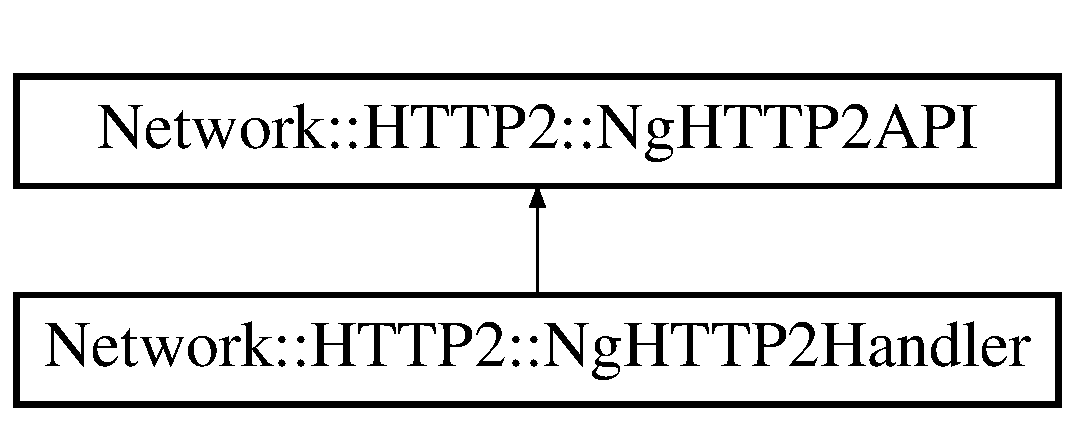
\includegraphics[height=2.000000cm]{d4/d0d/classNetwork_1_1HTTP2_1_1NgHTTP2Handler}
\end{center}
\end{figure}
\subsection*{Public Member Functions}
\begin{DoxyCompactItemize}
\item 
void \hyperlink{classNetwork_1_1HTTP2_1_1NgHTTP2Handler_a8fda32f531a6a3946dc861b06c519c95}{initialize} (\hyperlink{structNetwork_1_1HTTP2_1_1HTTP2HandlerResponse}{H\+T\+T\+P2\+Handler\+Response} $\ast$response, \hyperlink{classNetwork_1_1HTTP2_1_1NgHTTP2ResponseManager}{Ng\+H\+T\+T\+P2\+Response\+Manager} $\ast$manager)  throw (std\+::exception)
\begin{DoxyCompactList}\small\item\em Initialize. \end{DoxyCompactList}\item 
void \hyperlink{classNetwork_1_1HTTP2_1_1NgHTTP2Handler_a2384e4c12557cd181915dd33775b8a1a}{set\+Uri} (const char $\ast$uri)  throw ( std\+::exception )
\begin{DoxyCompactList}\small\item\em set\+Uri \end{DoxyCompactList}\item 
void \hyperlink{classNetwork_1_1HTTP2_1_1NgHTTP2Handler_af86bb397ae186757cd84d74954471e43}{set\+Port} (uint16\+\_\+t port)  throw ( std\+::exception )
\begin{DoxyCompactList}\small\item\em set\+Port \end{DoxyCompactList}\item 
void \hyperlink{classNetwork_1_1HTTP2_1_1NgHTTP2Handler_add84d25ff765f24e971b1c3177ef17a8}{set\+Response\+Manager} (\hyperlink{classNetwork_1_1HTTP2_1_1NgHTTP2ResponseManager}{Ng\+H\+T\+T\+P2\+Response\+Manager} $\ast$response\+\_\+manager)
\begin{DoxyCompactList}\small\item\em set\+Response\+Manager \end{DoxyCompactList}\item 
void \hyperlink{classNetwork_1_1HTTP2_1_1NgHTTP2Handler_a71d2ba66b9296604b81c440d1c54f670}{set\+Request\+Header} (nghttp2\+\_\+nv $\ast$ptr, size\+\_\+t size)  throw ( std\+::exception )
\begin{DoxyCompactList}\small\item\em set\+Header \end{DoxyCompactList}\item 
void \hyperlink{classNetwork_1_1HTTP2_1_1NgHTTP2Handler_acfa6474084f1a11dd9026ea8078d6b96}{set\+Request\+Source} (const std\+::string source)  throw ( std\+::exception )
\begin{DoxyCompactList}\small\item\em set\+Request\+Multipart \end{DoxyCompactList}\item 
void \hyperlink{classNetwork_1_1HTTP2_1_1NgHTTP2Handler_a0ffcd7addf3ea2dc9467312e3a45efff}{perform} (void)  throw ( std\+::exception )
\begin{DoxyCompactList}\small\item\em perform \end{DoxyCompactList}\item 
void \hyperlink{classNetwork_1_1HTTP2_1_1NgHTTP2Handler_a9ab6663ad62320d8588733aa9f467ace}{clean\+Up} (void)  throw (std\+::exception )
\begin{DoxyCompactList}\small\item\em Clean\+Up. \end{DoxyCompactList}\end{DoxyCompactItemize}
\subsection*{Static Protected Member Functions}
\begin{DoxyCompactItemize}
\item 
\mbox{\Hypertarget{classNetwork_1_1HTTP2_1_1NgHTTP2Handler_ae42b5d3aca9bc746770bb73af2a0f727}\label{classNetwork_1_1HTTP2_1_1NgHTTP2Handler_ae42b5d3aca9bc746770bb73af2a0f727}} 
static void {\bfseries on\+Response\+Header\+Event} (const void $\ast$name, size\+\_\+t name\+\_\+size, const void $\ast$value, size\+\_\+t value\+\_\+size, void $\ast$userdata)
\item 
\mbox{\Hypertarget{classNetwork_1_1HTTP2_1_1NgHTTP2Handler_acbed6056981ee0302bd24c86d1985319}\label{classNetwork_1_1HTTP2_1_1NgHTTP2Handler_acbed6056981ee0302bd24c86d1985319}} 
static void {\bfseries on\+Response\+Body\+Event} (void $\ast$content, size\+\_\+t size, void $\ast$userdata)
\end{DoxyCompactItemize}
\subsection*{Protected Attributes}
\begin{DoxyCompactItemize}
\item 
\mbox{\Hypertarget{classNetwork_1_1HTTP2_1_1NgHTTP2Handler_a9029be1f977fe05fa61e6c594682bf87}\label{classNetwork_1_1HTTP2_1_1NgHTTP2Handler_a9029be1f977fe05fa61e6c594682bf87}} 
\hyperlink{structNetwork_1_1HTTP2_1_1HTTP2HandlerSession}{H\+T\+T\+P2\+Handler\+Session} $\ast$ {\bfseries m\+\_\+session}
\item 
\mbox{\Hypertarget{classNetwork_1_1HTTP2_1_1NgHTTP2Handler_ab7de10d19b7ea978b7e55ecc6a0edc32}\label{classNetwork_1_1HTTP2_1_1NgHTTP2Handler_ab7de10d19b7ea978b7e55ecc6a0edc32}} 
\hyperlink{structNetwork_1_1HTTP2_1_1HTTP2HandlerResponse}{H\+T\+T\+P2\+Handler\+Response} $\ast$ {\bfseries m\+\_\+session\+\_\+response}
\item 
\mbox{\Hypertarget{classNetwork_1_1HTTP2_1_1NgHTTP2Handler_a2cf599837cab36282fe43974cbc0083a}\label{classNetwork_1_1HTTP2_1_1NgHTTP2Handler_a2cf599837cab36282fe43974cbc0083a}} 
\hyperlink{structNetwork_1_1HTTP2_1_1HTTP2HandlerResponseManagement}{H\+T\+T\+P2\+Handler\+Response\+Management} $\ast$ {\bfseries m\+\_\+session\+\_\+response\+\_\+management}
\item 
\mbox{\Hypertarget{classNetwork_1_1HTTP2_1_1NgHTTP2Handler_addf66405fdf0ed01d607bf43e559d31e}\label{classNetwork_1_1HTTP2_1_1NgHTTP2Handler_addf66405fdf0ed01d607bf43e559d31e}} 
\hyperlink{classNetwork_1_1HTTP2_1_1NgHTTP2ResponseManager}{Ng\+H\+T\+T\+P2\+Response\+Manager} $\ast$ {\bfseries m\+\_\+response\+\_\+manager}
\item 
\mbox{\Hypertarget{classNetwork_1_1HTTP2_1_1NgHTTP2Handler_a4b5d20e7eb960eb4e277cd1a07e2e9a3}\label{classNetwork_1_1HTTP2_1_1NgHTTP2Handler_a4b5d20e7eb960eb4e277cd1a07e2e9a3}} 
nghttp2\+\_\+nv $\ast$ {\bfseries m\+\_\+header\+\_\+copy}
\end{DoxyCompactItemize}


\subsection{Member Function Documentation}
\mbox{\Hypertarget{classNetwork_1_1HTTP2_1_1NgHTTP2Handler_a9ab6663ad62320d8588733aa9f467ace}\label{classNetwork_1_1HTTP2_1_1NgHTTP2Handler_a9ab6663ad62320d8588733aa9f467ace}} 
\index{Network\+::\+H\+T\+T\+P2\+::\+Ng\+H\+T\+T\+P2\+Handler@{Network\+::\+H\+T\+T\+P2\+::\+Ng\+H\+T\+T\+P2\+Handler}!clean\+Up@{clean\+Up}}
\index{clean\+Up@{clean\+Up}!Network\+::\+H\+T\+T\+P2\+::\+Ng\+H\+T\+T\+P2\+Handler@{Network\+::\+H\+T\+T\+P2\+::\+Ng\+H\+T\+T\+P2\+Handler}}
\subsubsection{\texorpdfstring{clean\+Up()}{cleanUp()}}
{\footnotesize\ttfamily void Ng\+H\+T\+T\+P2\+Handler\+::clean\+Up (\begin{DoxyParamCaption}\item[{void}]{ }\end{DoxyParamCaption}) throw  std\+::exception) }



Clean\+Up. 

destroy http2 session \mbox{\Hypertarget{classNetwork_1_1HTTP2_1_1NgHTTP2Handler_a8fda32f531a6a3946dc861b06c519c95}\label{classNetwork_1_1HTTP2_1_1NgHTTP2Handler_a8fda32f531a6a3946dc861b06c519c95}} 
\index{Network\+::\+H\+T\+T\+P2\+::\+Ng\+H\+T\+T\+P2\+Handler@{Network\+::\+H\+T\+T\+P2\+::\+Ng\+H\+T\+T\+P2\+Handler}!initialize@{initialize}}
\index{initialize@{initialize}!Network\+::\+H\+T\+T\+P2\+::\+Ng\+H\+T\+T\+P2\+Handler@{Network\+::\+H\+T\+T\+P2\+::\+Ng\+H\+T\+T\+P2\+Handler}}
\subsubsection{\texorpdfstring{initialize()}{initialize()}}
{\footnotesize\ttfamily void Ng\+H\+T\+T\+P2\+Handler\+::initialize (\begin{DoxyParamCaption}\item[{\hyperlink{structNetwork_1_1HTTP2_1_1HTTP2HandlerResponse}{H\+T\+T\+P2\+Handler\+Response} $\ast$}]{response,  }\item[{\hyperlink{classNetwork_1_1HTTP2_1_1NgHTTP2ResponseManager}{Ng\+H\+T\+T\+P2\+Response\+Manager} $\ast$}]{manager }\end{DoxyParamCaption}) throw  std\+::exception) }



Initialize. 

init http2 session \mbox{\Hypertarget{classNetwork_1_1HTTP2_1_1NgHTTP2Handler_a0ffcd7addf3ea2dc9467312e3a45efff}\label{classNetwork_1_1HTTP2_1_1NgHTTP2Handler_a0ffcd7addf3ea2dc9467312e3a45efff}} 
\index{Network\+::\+H\+T\+T\+P2\+::\+Ng\+H\+T\+T\+P2\+Handler@{Network\+::\+H\+T\+T\+P2\+::\+Ng\+H\+T\+T\+P2\+Handler}!perform@{perform}}
\index{perform@{perform}!Network\+::\+H\+T\+T\+P2\+::\+Ng\+H\+T\+T\+P2\+Handler@{Network\+::\+H\+T\+T\+P2\+::\+Ng\+H\+T\+T\+P2\+Handler}}
\subsubsection{\texorpdfstring{perform()}{perform()}}
{\footnotesize\ttfamily void Ng\+H\+T\+T\+P2\+Handler\+::perform (\begin{DoxyParamCaption}\item[{void}]{ }\end{DoxyParamCaption}) throw  std\+::exception) }



perform 

send data to server \begin{DoxyReturn}{Returns}

\end{DoxyReturn}
\mbox{\Hypertarget{classNetwork_1_1HTTP2_1_1NgHTTP2Handler_af86bb397ae186757cd84d74954471e43}\label{classNetwork_1_1HTTP2_1_1NgHTTP2Handler_af86bb397ae186757cd84d74954471e43}} 
\index{Network\+::\+H\+T\+T\+P2\+::\+Ng\+H\+T\+T\+P2\+Handler@{Network\+::\+H\+T\+T\+P2\+::\+Ng\+H\+T\+T\+P2\+Handler}!set\+Port@{set\+Port}}
\index{set\+Port@{set\+Port}!Network\+::\+H\+T\+T\+P2\+::\+Ng\+H\+T\+T\+P2\+Handler@{Network\+::\+H\+T\+T\+P2\+::\+Ng\+H\+T\+T\+P2\+Handler}}
\subsubsection{\texorpdfstring{set\+Port()}{setPort()}}
{\footnotesize\ttfamily void Ng\+H\+T\+T\+P2\+Handler\+::set\+Port (\begin{DoxyParamCaption}\item[{uint16\+\_\+t}]{port }\end{DoxyParamCaption}) throw  std\+::exception) }



set\+Port 

Set Server Port 
\begin{DoxyParams}{Parameters}
{\em port} & Default\+: 443 \\
\hline
\end{DoxyParams}
\mbox{\Hypertarget{classNetwork_1_1HTTP2_1_1NgHTTP2Handler_a71d2ba66b9296604b81c440d1c54f670}\label{classNetwork_1_1HTTP2_1_1NgHTTP2Handler_a71d2ba66b9296604b81c440d1c54f670}} 
\index{Network\+::\+H\+T\+T\+P2\+::\+Ng\+H\+T\+T\+P2\+Handler@{Network\+::\+H\+T\+T\+P2\+::\+Ng\+H\+T\+T\+P2\+Handler}!set\+Request\+Header@{set\+Request\+Header}}
\index{set\+Request\+Header@{set\+Request\+Header}!Network\+::\+H\+T\+T\+P2\+::\+Ng\+H\+T\+T\+P2\+Handler@{Network\+::\+H\+T\+T\+P2\+::\+Ng\+H\+T\+T\+P2\+Handler}}
\subsubsection{\texorpdfstring{set\+Request\+Header()}{setRequestHeader()}}
{\footnotesize\ttfamily void Ng\+H\+T\+T\+P2\+Handler\+::set\+Request\+Header (\begin{DoxyParamCaption}\item[{nghttp2\+\_\+nv $\ast$}]{ptr,  }\item[{size\+\_\+t}]{size }\end{DoxyParamCaption}) throw  std\+::exception) }



set\+Header 

Set H\+T\+T\+P2 Request Header \mbox{\Hypertarget{classNetwork_1_1HTTP2_1_1NgHTTP2Handler_acfa6474084f1a11dd9026ea8078d6b96}\label{classNetwork_1_1HTTP2_1_1NgHTTP2Handler_acfa6474084f1a11dd9026ea8078d6b96}} 
\index{Network\+::\+H\+T\+T\+P2\+::\+Ng\+H\+T\+T\+P2\+Handler@{Network\+::\+H\+T\+T\+P2\+::\+Ng\+H\+T\+T\+P2\+Handler}!set\+Request\+Source@{set\+Request\+Source}}
\index{set\+Request\+Source@{set\+Request\+Source}!Network\+::\+H\+T\+T\+P2\+::\+Ng\+H\+T\+T\+P2\+Handler@{Network\+::\+H\+T\+T\+P2\+::\+Ng\+H\+T\+T\+P2\+Handler}}
\subsubsection{\texorpdfstring{set\+Request\+Source()}{setRequestSource()}}
{\footnotesize\ttfamily void Ng\+H\+T\+T\+P2\+Handler\+::set\+Request\+Source (\begin{DoxyParamCaption}\item[{const std\+::string}]{source }\end{DoxyParamCaption}) throw  std\+::exception) }



set\+Request\+Multipart 

Set H\+T\+T\+P2 Request Body Content 
\begin{DoxyParams}{Parameters}
{\em fd} & \+: File\+Descriptor \\
\hline
\end{DoxyParams}
\mbox{\Hypertarget{classNetwork_1_1HTTP2_1_1NgHTTP2Handler_add84d25ff765f24e971b1c3177ef17a8}\label{classNetwork_1_1HTTP2_1_1NgHTTP2Handler_add84d25ff765f24e971b1c3177ef17a8}} 
\index{Network\+::\+H\+T\+T\+P2\+::\+Ng\+H\+T\+T\+P2\+Handler@{Network\+::\+H\+T\+T\+P2\+::\+Ng\+H\+T\+T\+P2\+Handler}!set\+Response\+Manager@{set\+Response\+Manager}}
\index{set\+Response\+Manager@{set\+Response\+Manager}!Network\+::\+H\+T\+T\+P2\+::\+Ng\+H\+T\+T\+P2\+Handler@{Network\+::\+H\+T\+T\+P2\+::\+Ng\+H\+T\+T\+P2\+Handler}}
\subsubsection{\texorpdfstring{set\+Response\+Manager()}{setResponseManager()}}
{\footnotesize\ttfamily void Ng\+H\+T\+T\+P2\+Handler\+::set\+Response\+Manager (\begin{DoxyParamCaption}\item[{\hyperlink{classNetwork_1_1HTTP2_1_1NgHTTP2ResponseManager}{Ng\+H\+T\+T\+P2\+Response\+Manager} $\ast$}]{response\+\_\+manager }\end{DoxyParamCaption})}



set\+Response\+Manager 


\begin{DoxyParams}{Parameters}
{\em response\+\_\+manager} & \\
\hline
\end{DoxyParams}
\mbox{\Hypertarget{classNetwork_1_1HTTP2_1_1NgHTTP2Handler_a2384e4c12557cd181915dd33775b8a1a}\label{classNetwork_1_1HTTP2_1_1NgHTTP2Handler_a2384e4c12557cd181915dd33775b8a1a}} 
\index{Network\+::\+H\+T\+T\+P2\+::\+Ng\+H\+T\+T\+P2\+Handler@{Network\+::\+H\+T\+T\+P2\+::\+Ng\+H\+T\+T\+P2\+Handler}!set\+Uri@{set\+Uri}}
\index{set\+Uri@{set\+Uri}!Network\+::\+H\+T\+T\+P2\+::\+Ng\+H\+T\+T\+P2\+Handler@{Network\+::\+H\+T\+T\+P2\+::\+Ng\+H\+T\+T\+P2\+Handler}}
\subsubsection{\texorpdfstring{set\+Uri()}{setUri()}}
{\footnotesize\ttfamily void Ng\+H\+T\+T\+P2\+Handler\+::set\+Uri (\begin{DoxyParamCaption}\item[{const char $\ast$}]{uri }\end{DoxyParamCaption}) throw  std\+::exception) }



set\+Uri 

Set U\+RI \+: \href{https://example.de}{\tt https\+://example.\+de} without https only example.\+de 
\begin{DoxyParams}{Parameters}
{\em uri} & \\
\hline
\end{DoxyParams}


The documentation for this class was generated from the following files\+:\begin{DoxyCompactItemize}
\item 
/home/mutzi/progs/linux\+\_\+workspace/alexa-\/avs-\/prototype/src/include/nghttp2handler.\+h\item 
/home/mutzi/progs/linux\+\_\+workspace/alexa-\/avs-\/prototype/src/nghttp2handler.\+cpp\end{DoxyCompactItemize}

\hypertarget{classNetwork_1_1HTTP2_1_1NgHTTP2MultiplexHandler}{}\section{Network\+:\+:H\+T\+T\+P2\+:\+:Ng\+H\+T\+T\+P2\+Multiplex\+Handler Class Reference}
\label{classNetwork_1_1HTTP2_1_1NgHTTP2MultiplexHandler}\index{Network\+::\+H\+T\+T\+P2\+::\+Ng\+H\+T\+T\+P2\+Multiplex\+Handler@{Network\+::\+H\+T\+T\+P2\+::\+Ng\+H\+T\+T\+P2\+Multiplex\+Handler}}
Inheritance diagram for Network\+:\+:H\+T\+T\+P2\+:\+:Ng\+H\+T\+T\+P2\+Multiplex\+Handler\+:\begin{figure}[H]
\begin{center}
\leavevmode
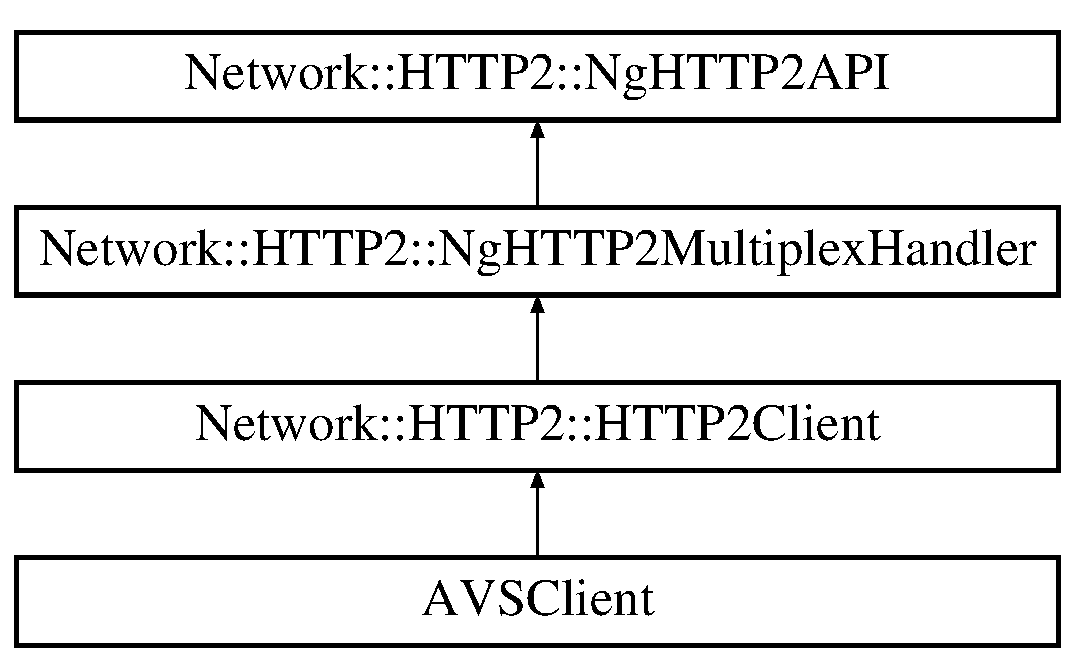
\includegraphics[height=4.000000cm]{d0/dab/classNetwork_1_1HTTP2_1_1NgHTTP2MultiplexHandler}
\end{center}
\end{figure}
\subsection*{Public Member Functions}
\begin{DoxyCompactItemize}
\item 
void \hyperlink{classNetwork_1_1HTTP2_1_1NgHTTP2MultiplexHandler_a430b5ddd0dd77ebde81d201277216aa4}{initialize} (\hyperlink{structNetwork_1_1HTTP2_1_1HTTP2HandlerResponse}{H\+T\+T\+P2\+Handler\+Response} $\ast$response, \hyperlink{classNetwork_1_1HTTP2_1_1NgHTTP2ResponseManager}{Ng\+H\+T\+T\+P2\+Response\+Manager} $\ast$manager)  throw (std\+::exception)
\begin{DoxyCompactList}\small\item\em Initialize. \end{DoxyCompactList}\item 
\mbox{\Hypertarget{classNetwork_1_1HTTP2_1_1NgHTTP2MultiplexHandler_a502967cc6e72b0cab674e9b02d4c91a2}\label{classNetwork_1_1HTTP2_1_1NgHTTP2MultiplexHandler_a502967cc6e72b0cab674e9b02d4c91a2}} 
void {\bfseries initiate\+Stream} (const char $\ast$uri, nghttp2\+\_\+nv $\ast$header\+\_\+data, size\+\_\+t arr\+\_\+len, int $\ast$status)
\item 
\mbox{\Hypertarget{classNetwork_1_1HTTP2_1_1NgHTTP2MultiplexHandler_a24522d32d46883373a1602fb4f9188c2}\label{classNetwork_1_1HTTP2_1_1NgHTTP2MultiplexHandler_a24522d32d46883373a1602fb4f9188c2}} 
void {\bfseries create\+New\+Stream} (\hyperlink{structNetwork_1_1HTTP2_1_1StreamQueueData}{Stream\+Queue\+Data} $\ast$data, struct event\+\_\+base $\ast$evbase)
\item 
void \hyperlink{classNetwork_1_1HTTP2_1_1NgHTTP2MultiplexHandler_a5c052bed83cde53d1c6c0a18bc9f1e33}{set\+Uri} (const char $\ast$uri)  throw ( std\+::exception )
\begin{DoxyCompactList}\small\item\em set\+Uri \end{DoxyCompactList}\item 
void \hyperlink{classNetwork_1_1HTTP2_1_1NgHTTP2MultiplexHandler_a9f804c1d683748a166042c834fd55203}{set\+Port} (uint16\+\_\+t port)  throw ( std\+::exception )
\begin{DoxyCompactList}\small\item\em set\+Port \end{DoxyCompactList}\item 
void \hyperlink{classNetwork_1_1HTTP2_1_1NgHTTP2MultiplexHandler_a084530d95344321d1d1a3765e18d2eff}{clean\+Up} (void)  throw (std\+::exception )
\begin{DoxyCompactList}\small\item\em Clean\+Up. \end{DoxyCompactList}\item 
virtual void \hyperlink{classNetwork_1_1HTTP2_1_1NgHTTP2MultiplexHandler_a95e9df9737af24d79894320e8cb343de}{stream\+\_\+loop} (struct event\+\_\+base $\ast$evbase)=0
\begin{DoxyCompactList}\small\item\em stream\+\_\+loop \end{DoxyCompactList}\end{DoxyCompactItemize}
\subsection*{Static Protected Member Functions}
\begin{DoxyCompactItemize}
\item 
\mbox{\Hypertarget{classNetwork_1_1HTTP2_1_1NgHTTP2MultiplexHandler_a7b285c14acbc9d1afdc3b6fa39d2ba66}\label{classNetwork_1_1HTTP2_1_1NgHTTP2MultiplexHandler_a7b285c14acbc9d1afdc3b6fa39d2ba66}} 
static void {\bfseries on\+Response\+Header\+Event} (const void $\ast$name, size\+\_\+t name\+\_\+size, const void $\ast$value, size\+\_\+t value\+\_\+size, void $\ast$userdata)
\item 
\mbox{\Hypertarget{classNetwork_1_1HTTP2_1_1NgHTTP2MultiplexHandler_a4c1e15026f66931b58db5edaa299981c}\label{classNetwork_1_1HTTP2_1_1NgHTTP2MultiplexHandler_a4c1e15026f66931b58db5edaa299981c}} 
static void {\bfseries on\+Response\+Body\+Event} (void $\ast$content, size\+\_\+t size, void $\ast$userdata)
\end{DoxyCompactItemize}
\subsection*{Protected Attributes}
\begin{DoxyCompactItemize}
\item 
\mbox{\Hypertarget{classNetwork_1_1HTTP2_1_1NgHTTP2MultiplexHandler_acf4274648cd3c85bbd4fe65e1dffa01f}\label{classNetwork_1_1HTTP2_1_1NgHTTP2MultiplexHandler_acf4274648cd3c85bbd4fe65e1dffa01f}} 
\hyperlink{structNetwork_1_1HTTP2_1_1HTTP2HandlerSession}{H\+T\+T\+P2\+Handler\+Session} $\ast$ {\bfseries m\+\_\+session}
\item 
\mbox{\Hypertarget{classNetwork_1_1HTTP2_1_1NgHTTP2MultiplexHandler_a8aae36038830c947075fb97d29895b2f}\label{classNetwork_1_1HTTP2_1_1NgHTTP2MultiplexHandler_a8aae36038830c947075fb97d29895b2f}} 
\hyperlink{structNetwork_1_1HTTP2_1_1HTTP2HandlerResponseManagement}{H\+T\+T\+P2\+Handler\+Response\+Management} $\ast$ {\bfseries m\+\_\+session\+\_\+response\+\_\+management}
\end{DoxyCompactItemize}


\subsection{Member Function Documentation}
\mbox{\Hypertarget{classNetwork_1_1HTTP2_1_1NgHTTP2MultiplexHandler_a084530d95344321d1d1a3765e18d2eff}\label{classNetwork_1_1HTTP2_1_1NgHTTP2MultiplexHandler_a084530d95344321d1d1a3765e18d2eff}} 
\index{Network\+::\+H\+T\+T\+P2\+::\+Ng\+H\+T\+T\+P2\+Multiplex\+Handler@{Network\+::\+H\+T\+T\+P2\+::\+Ng\+H\+T\+T\+P2\+Multiplex\+Handler}!clean\+Up@{clean\+Up}}
\index{clean\+Up@{clean\+Up}!Network\+::\+H\+T\+T\+P2\+::\+Ng\+H\+T\+T\+P2\+Multiplex\+Handler@{Network\+::\+H\+T\+T\+P2\+::\+Ng\+H\+T\+T\+P2\+Multiplex\+Handler}}
\subsubsection{\texorpdfstring{clean\+Up()}{cleanUp()}}
{\footnotesize\ttfamily void Ng\+H\+T\+T\+P2\+Multiplex\+Handler\+::clean\+Up (\begin{DoxyParamCaption}\item[{void}]{ }\end{DoxyParamCaption}) throw  std\+::exception) }



Clean\+Up. 

destroy http2 session \mbox{\Hypertarget{classNetwork_1_1HTTP2_1_1NgHTTP2MultiplexHandler_a430b5ddd0dd77ebde81d201277216aa4}\label{classNetwork_1_1HTTP2_1_1NgHTTP2MultiplexHandler_a430b5ddd0dd77ebde81d201277216aa4}} 
\index{Network\+::\+H\+T\+T\+P2\+::\+Ng\+H\+T\+T\+P2\+Multiplex\+Handler@{Network\+::\+H\+T\+T\+P2\+::\+Ng\+H\+T\+T\+P2\+Multiplex\+Handler}!initialize@{initialize}}
\index{initialize@{initialize}!Network\+::\+H\+T\+T\+P2\+::\+Ng\+H\+T\+T\+P2\+Multiplex\+Handler@{Network\+::\+H\+T\+T\+P2\+::\+Ng\+H\+T\+T\+P2\+Multiplex\+Handler}}
\subsubsection{\texorpdfstring{initialize()}{initialize()}}
{\footnotesize\ttfamily void Ng\+H\+T\+T\+P2\+Multiplex\+Handler\+::initialize (\begin{DoxyParamCaption}\item[{\hyperlink{structNetwork_1_1HTTP2_1_1HTTP2HandlerResponse}{H\+T\+T\+P2\+Handler\+Response} $\ast$}]{response,  }\item[{\hyperlink{classNetwork_1_1HTTP2_1_1NgHTTP2ResponseManager}{Ng\+H\+T\+T\+P2\+Response\+Manager} $\ast$}]{manager }\end{DoxyParamCaption}) throw  std\+::exception) }



Initialize. 

init http2 session \mbox{\Hypertarget{classNetwork_1_1HTTP2_1_1NgHTTP2MultiplexHandler_a9f804c1d683748a166042c834fd55203}\label{classNetwork_1_1HTTP2_1_1NgHTTP2MultiplexHandler_a9f804c1d683748a166042c834fd55203}} 
\index{Network\+::\+H\+T\+T\+P2\+::\+Ng\+H\+T\+T\+P2\+Multiplex\+Handler@{Network\+::\+H\+T\+T\+P2\+::\+Ng\+H\+T\+T\+P2\+Multiplex\+Handler}!set\+Port@{set\+Port}}
\index{set\+Port@{set\+Port}!Network\+::\+H\+T\+T\+P2\+::\+Ng\+H\+T\+T\+P2\+Multiplex\+Handler@{Network\+::\+H\+T\+T\+P2\+::\+Ng\+H\+T\+T\+P2\+Multiplex\+Handler}}
\subsubsection{\texorpdfstring{set\+Port()}{setPort()}}
{\footnotesize\ttfamily void Ng\+H\+T\+T\+P2\+Multiplex\+Handler\+::set\+Port (\begin{DoxyParamCaption}\item[{uint16\+\_\+t}]{port }\end{DoxyParamCaption}) throw  std\+::exception) }



set\+Port 

Set Server Port 
\begin{DoxyParams}{Parameters}
{\em port} & Default\+: 443 \\
\hline
\end{DoxyParams}
\mbox{\Hypertarget{classNetwork_1_1HTTP2_1_1NgHTTP2MultiplexHandler_a5c052bed83cde53d1c6c0a18bc9f1e33}\label{classNetwork_1_1HTTP2_1_1NgHTTP2MultiplexHandler_a5c052bed83cde53d1c6c0a18bc9f1e33}} 
\index{Network\+::\+H\+T\+T\+P2\+::\+Ng\+H\+T\+T\+P2\+Multiplex\+Handler@{Network\+::\+H\+T\+T\+P2\+::\+Ng\+H\+T\+T\+P2\+Multiplex\+Handler}!set\+Uri@{set\+Uri}}
\index{set\+Uri@{set\+Uri}!Network\+::\+H\+T\+T\+P2\+::\+Ng\+H\+T\+T\+P2\+Multiplex\+Handler@{Network\+::\+H\+T\+T\+P2\+::\+Ng\+H\+T\+T\+P2\+Multiplex\+Handler}}
\subsubsection{\texorpdfstring{set\+Uri()}{setUri()}}
{\footnotesize\ttfamily void Ng\+H\+T\+T\+P2\+Multiplex\+Handler\+::set\+Uri (\begin{DoxyParamCaption}\item[{const char $\ast$}]{uri }\end{DoxyParamCaption}) throw  std\+::exception) }



set\+Uri 

Set U\+RI \+: \href{https://example.de}{\tt https\+://example.\+de} without https only example.\+de 
\begin{DoxyParams}{Parameters}
{\em uri} & \\
\hline
\end{DoxyParams}
\mbox{\Hypertarget{classNetwork_1_1HTTP2_1_1NgHTTP2MultiplexHandler_a95e9df9737af24d79894320e8cb343de}\label{classNetwork_1_1HTTP2_1_1NgHTTP2MultiplexHandler_a95e9df9737af24d79894320e8cb343de}} 
\index{Network\+::\+H\+T\+T\+P2\+::\+Ng\+H\+T\+T\+P2\+Multiplex\+Handler@{Network\+::\+H\+T\+T\+P2\+::\+Ng\+H\+T\+T\+P2\+Multiplex\+Handler}!stream\+\_\+loop@{stream\+\_\+loop}}
\index{stream\+\_\+loop@{stream\+\_\+loop}!Network\+::\+H\+T\+T\+P2\+::\+Ng\+H\+T\+T\+P2\+Multiplex\+Handler@{Network\+::\+H\+T\+T\+P2\+::\+Ng\+H\+T\+T\+P2\+Multiplex\+Handler}}
\subsubsection{\texorpdfstring{stream\+\_\+loop()}{stream\_loop()}}
{\footnotesize\ttfamily virtual void Network\+::\+H\+T\+T\+P2\+::\+Ng\+H\+T\+T\+P2\+Multiplex\+Handler\+::stream\+\_\+loop (\begin{DoxyParamCaption}\item[{struct event\+\_\+base $\ast$}]{evbase }\end{DoxyParamCaption})\hspace{0.3cm}{\ttfamily [pure virtual]}}



stream\+\_\+loop 

override it ... 
\begin{DoxyParams}{Parameters}
{\em handler} & \\
\hline
\end{DoxyParams}


Implemented in \hyperlink{classNetwork_1_1HTTP2_1_1HTTP2Client_a5c5cd10569102998104f2124a3c7a119}{Network\+::\+H\+T\+T\+P2\+::\+H\+T\+T\+P2\+Client}.



The documentation for this class was generated from the following files\+:\begin{DoxyCompactItemize}
\item 
/home/mutzi/progs/linux\+\_\+workspace/alexa-\/avs-\/prototype/src/include/nghttp2multiplexhandler.\+h\item 
/home/mutzi/progs/linux\+\_\+workspace/alexa-\/avs-\/prototype/src/nghttp2multiplexhandler.\+cpp\end{DoxyCompactItemize}

\hypertarget{classNetwork_1_1HTTP2_1_1NgHTTP2ResponseListener}{}\section{Network\+:\+:H\+T\+T\+P2\+:\+:Ng\+H\+T\+T\+P2\+Response\+Listener Class Reference}
\label{classNetwork_1_1HTTP2_1_1NgHTTP2ResponseListener}\index{Network\+::\+H\+T\+T\+P2\+::\+Ng\+H\+T\+T\+P2\+Response\+Listener@{Network\+::\+H\+T\+T\+P2\+::\+Ng\+H\+T\+T\+P2\+Response\+Listener}}
Inheritance diagram for Network\+:\+:H\+T\+T\+P2\+:\+:Ng\+H\+T\+T\+P2\+Response\+Listener\+:\begin{figure}[H]
\begin{center}
\leavevmode
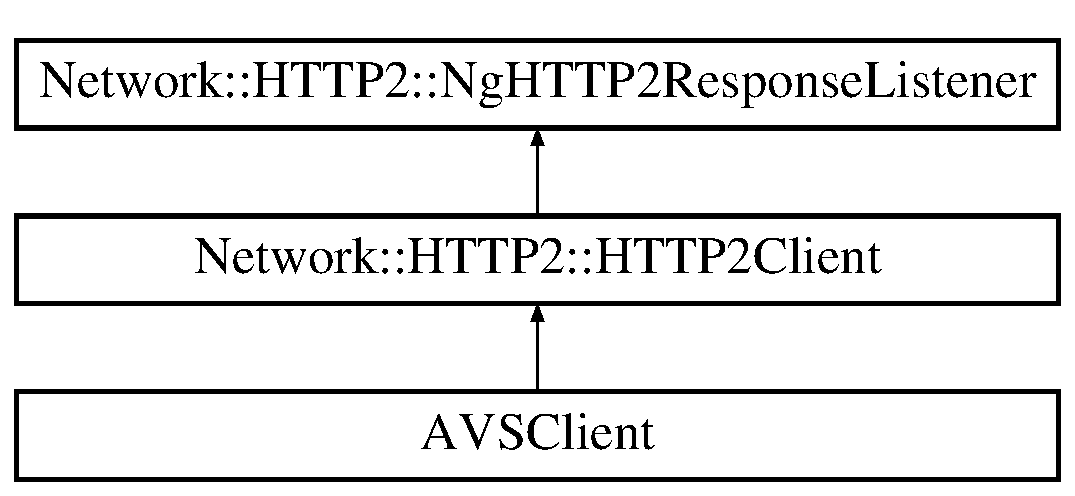
\includegraphics[height=3.000000cm]{d0/d27/classNetwork_1_1HTTP2_1_1NgHTTP2ResponseListener}
\end{center}
\end{figure}
\subsection*{Public Member Functions}
\begin{DoxyCompactItemize}
\item 
\mbox{\Hypertarget{classNetwork_1_1HTTP2_1_1NgHTTP2ResponseListener_a063ae0ea63ee29845b589cd23e97495a}\label{classNetwork_1_1HTTP2_1_1NgHTTP2ResponseListener_a063ae0ea63ee29845b589cd23e97495a}} 
virtual void {\bfseries on\+Response\+Event} (struct \hyperlink{structNetwork_1_1HTTP2_1_1HTTP2HandlerResponse}{H\+T\+T\+P2\+Handler\+Response} $\ast$response)=0
\item 
\mbox{\Hypertarget{classNetwork_1_1HTTP2_1_1NgHTTP2ResponseListener_a69e9cb5d6ffb457d8e41ed29e675ad46}\label{classNetwork_1_1HTTP2_1_1NgHTTP2ResponseListener_a69e9cb5d6ffb457d8e41ed29e675ad46}} 
virtual void {\bfseries on\+Response\+Header\+Status\+Event} (const char $\ast$status\+\_\+code)=0
\end{DoxyCompactItemize}


The documentation for this class was generated from the following file\+:\begin{DoxyCompactItemize}
\item 
/home/mutzi/progs/linux\+\_\+workspace/alexa-\/avs-\/prototype/src/include/nghttp2handler.\+h\end{DoxyCompactItemize}

\hypertarget{classNetwork_1_1HTTP2_1_1NgHTTP2ResponseManager}{}\section{Network\+:\+:H\+T\+T\+P2\+:\+:Ng\+H\+T\+T\+P2\+Response\+Manager Class Reference}
\label{classNetwork_1_1HTTP2_1_1NgHTTP2ResponseManager}\index{Network\+::\+H\+T\+T\+P2\+::\+Ng\+H\+T\+T\+P2\+Response\+Manager@{Network\+::\+H\+T\+T\+P2\+::\+Ng\+H\+T\+T\+P2\+Response\+Manager}}
\subsection*{Public Member Functions}
\begin{DoxyCompactItemize}
\item 
\mbox{\Hypertarget{classNetwork_1_1HTTP2_1_1NgHTTP2ResponseManager_a82a0ae30e4af2a82cdd5f27e863bc4a2}\label{classNetwork_1_1HTTP2_1_1NgHTTP2ResponseManager_a82a0ae30e4af2a82cdd5f27e863bc4a2}} 
void {\bfseries register\+Response\+Listener} (\hyperlink{classNetwork_1_1HTTP2_1_1NgHTTP2ResponseListener}{Ng\+H\+T\+T\+P2\+Response\+Listener} $\ast$listener)
\item 
\mbox{\Hypertarget{classNetwork_1_1HTTP2_1_1NgHTTP2ResponseManager_a655ae86a9ac8e0761bd2baf93ed64d6c}\label{classNetwork_1_1HTTP2_1_1NgHTTP2ResponseManager_a655ae86a9ac8e0761bd2baf93ed64d6c}} 
void {\bfseries create\+Response\+Event} (struct \hyperlink{structNetwork_1_1HTTP2_1_1HTTP2HandlerResponse}{H\+T\+T\+P2\+Handler\+Response} $\ast$response)
\item 
\mbox{\Hypertarget{classNetwork_1_1HTTP2_1_1NgHTTP2ResponseManager_ab7f32d52cc08a5ce69978c64dff33144}\label{classNetwork_1_1HTTP2_1_1NgHTTP2ResponseManager_ab7f32d52cc08a5ce69978c64dff33144}} 
void {\bfseries create\+Response\+Header\+Status\+Event} (const char $\ast$status\+\_\+code)
\end{DoxyCompactItemize}


The documentation for this class was generated from the following files\+:\begin{DoxyCompactItemize}
\item 
/home/mutzi/progs/linux\+\_\+workspace/alexa-\/avs-\/prototype/src/include/nghttp2responsemanager.\+h\item 
/home/mutzi/progs/linux\+\_\+workspace/alexa-\/avs-\/prototype/src/nghttp2responsemanager.\+cpp\end{DoxyCompactItemize}

\hypertarget{classnlohmann_1_1detail_1_1other__error}{}\section{nlohmann\+:\+:detail\+:\+:other\+\_\+error Class Reference}
\label{classnlohmann_1_1detail_1_1other__error}\index{nlohmann\+::detail\+::other\+\_\+error@{nlohmann\+::detail\+::other\+\_\+error}}


exception indicating other errors  




{\ttfamily \#include $<$nlohmann\+\_\+json.\+h$>$}

Inheritance diagram for nlohmann\+:\+:detail\+:\+:other\+\_\+error\+:\begin{figure}[H]
\begin{center}
\leavevmode
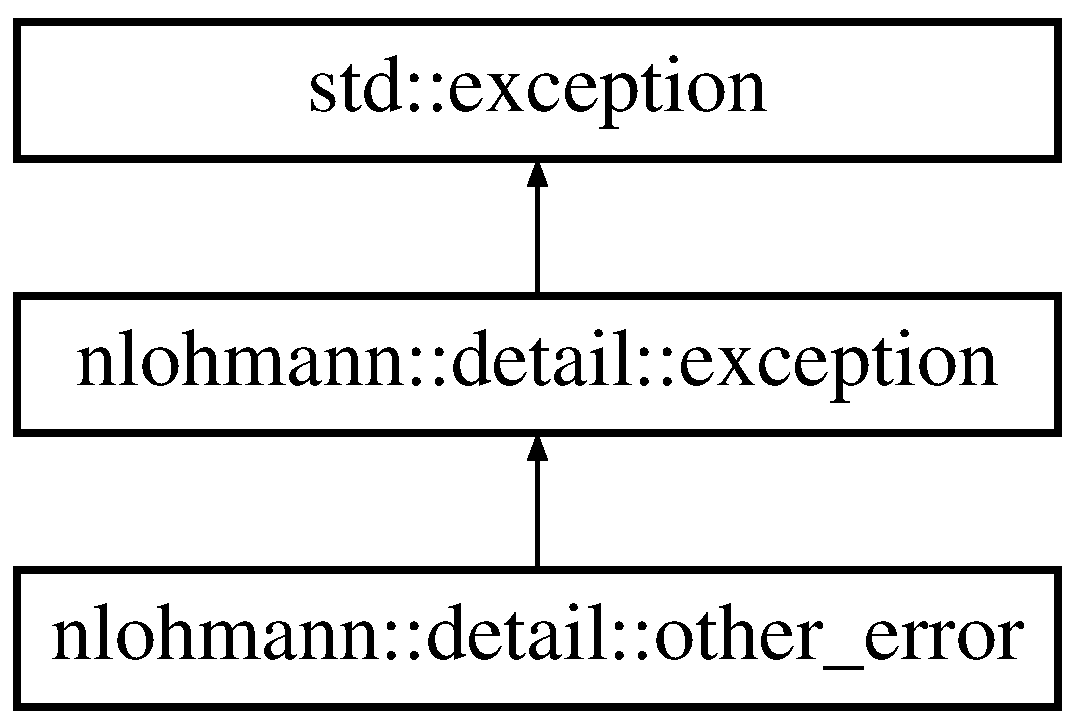
\includegraphics[height=3.000000cm]{d5/d1b/classnlohmann_1_1detail_1_1other__error}
\end{center}
\end{figure}
\subsection*{Static Public Member Functions}
\begin{DoxyCompactItemize}
\item 
\mbox{\Hypertarget{classnlohmann_1_1detail_1_1other__error_a1443f7682e7dd05144a577f0d3765c63}\label{classnlohmann_1_1detail_1_1other__error_a1443f7682e7dd05144a577f0d3765c63}} 
static \hyperlink{classnlohmann_1_1detail_1_1other__error}{other\+\_\+error} {\bfseries create} (int \hyperlink{classnlohmann_1_1detail_1_1exception_a0d4589a3fb54e81646d986c05efa3b9a}{id}, const \hyperlink{namespacenlohmann_1_1detail_a90aa5ef615aa8305e9ea20d8a947980fab45cffe084dd3d20d928bee85e7b0f21}{std\+::string} \&what\+\_\+arg)
\end{DoxyCompactItemize}
\subsection*{Additional Inherited Members}


\subsection{Detailed Description}
exception indicating other errors 

Exceptions have ids 5xx.

\tabulinesep=1mm
\begin{longtabu} spread 0pt [c]{*{3}{|X[-1]}|}
\hline
\rowcolor{\tableheadbgcolor}\textbf{ name / id }&\textbf{ example massage }&\textbf{ description  }\\\cline{1-3}
\endfirsthead
\hline
\endfoot
\hline
\rowcolor{\tableheadbgcolor}\textbf{ name / id }&\textbf{ example massage }&\textbf{ description  }\\\cline{1-3}
\endhead
json.\+exception.\+other\+\_\+error.\+501 &unsuccessful\+: \{\char`\"{}op\char`\"{}\+:\char`\"{}test\char`\"{},\char`\"{}path\char`\"{}\+:\char`\"{}/baz\char`\"{}, \char`\"{}value\char`\"{}\+:\char`\"{}bar\char`\"{}\} &A J\+S\+ON Patch operation \textquotesingle{}test\textquotesingle{} failed. The unsuccessful operation is also printed. \\\cline{1-3}
\end{longtabu}
\begin{DoxySince}{Since}
version 3.\+0.\+0 
\end{DoxySince}


The documentation for this class was generated from the following file\+:\begin{DoxyCompactItemize}
\item 
/home/mutzi/progs/linux\+\_\+workspace/alexa-\/avs-\/prototype/src/include/nlohmann\+\_\+json.\+h\end{DoxyCompactItemize}

\hypertarget{classnlohmann_1_1detail_1_1out__of__range}{}\section{nlohmann\+:\+:detail\+:\+:out\+\_\+of\+\_\+range Class Reference}
\label{classnlohmann_1_1detail_1_1out__of__range}\index{nlohmann\+::detail\+::out\+\_\+of\+\_\+range@{nlohmann\+::detail\+::out\+\_\+of\+\_\+range}}


exception indicating access out of the defined range  




{\ttfamily \#include $<$nlohmann\+\_\+json.\+h$>$}

Inheritance diagram for nlohmann\+:\+:detail\+:\+:out\+\_\+of\+\_\+range\+:\begin{figure}[H]
\begin{center}
\leavevmode
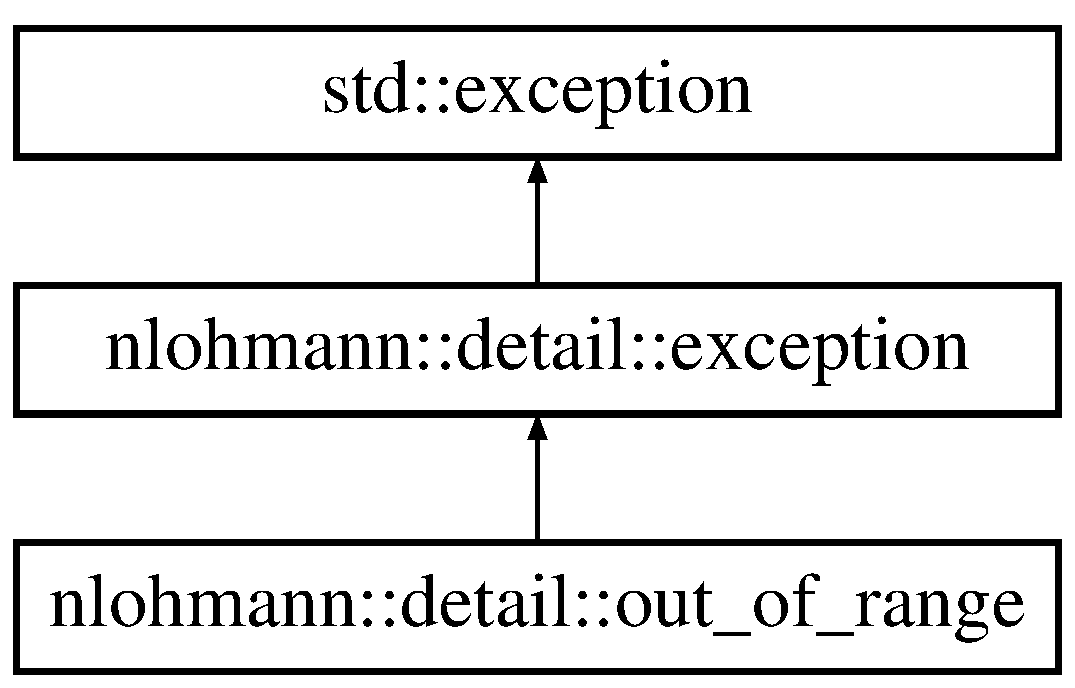
\includegraphics[height=3.000000cm]{d2/d67/classnlohmann_1_1detail_1_1out__of__range}
\end{center}
\end{figure}
\subsection*{Static Public Member Functions}
\begin{DoxyCompactItemize}
\item 
\mbox{\Hypertarget{classnlohmann_1_1detail_1_1out__of__range_a661c8a3af0caeb2621bfb7ae3a02c66b}\label{classnlohmann_1_1detail_1_1out__of__range_a661c8a3af0caeb2621bfb7ae3a02c66b}} 
static \hyperlink{classnlohmann_1_1detail_1_1out__of__range}{out\+\_\+of\+\_\+range} {\bfseries create} (int \hyperlink{classnlohmann_1_1detail_1_1exception_a0d4589a3fb54e81646d986c05efa3b9a}{id}, const \hyperlink{namespacenlohmann_1_1detail_a90aa5ef615aa8305e9ea20d8a947980fab45cffe084dd3d20d928bee85e7b0f21}{std\+::string} \&what\+\_\+arg)
\end{DoxyCompactItemize}
\subsection*{Additional Inherited Members}


\subsection{Detailed Description}
exception indicating access out of the defined range 

Exceptions have ids 4xx.

\tabulinesep=1mm
\begin{longtabu} spread 0pt [c]{*{3}{|X[-1]}|}
\hline
\rowcolor{\tableheadbgcolor}\textbf{ name / id }&\textbf{ example massage }&\textbf{ description  }\\\cline{1-3}
\endfirsthead
\hline
\endfoot
\hline
\rowcolor{\tableheadbgcolor}\textbf{ name / id }&\textbf{ example massage }&\textbf{ description  }\\\cline{1-3}
\endhead
json.\+exception.\+out\+\_\+of\+\_\+range.\+401 &array index 3 is out of range &The provided array index {\itshape i} is larger than {\itshape size-\/1}. \\\cline{1-3}
json.\+exception.\+out\+\_\+of\+\_\+range.\+402 &array index \textquotesingle{}-\/\textquotesingle{} (3) is out of range &The special array index {\ttfamily -\/} in a J\+S\+ON Pointer never describes a valid element of the array, but the index past the end. That is, it can only be used to add elements at this position, but not to read it. \\\cline{1-3}
json.\+exception.\+out\+\_\+of\+\_\+range.\+403 &key \textquotesingle{}foo\textquotesingle{} not found &The provided key was not found in the J\+S\+ON object. \\\cline{1-3}
json.\+exception.\+out\+\_\+of\+\_\+range.\+404 &unresolved reference token \textquotesingle{}foo\textquotesingle{} &A reference token in a J\+S\+ON Pointer could not be resolved. \\\cline{1-3}
json.\+exception.\+out\+\_\+of\+\_\+range.\+405 &J\+S\+ON pointer has no parent &The J\+S\+ON Patch operations \textquotesingle{}remove\textquotesingle{} and \textquotesingle{}add\textquotesingle{} can not be applied to the root element of the J\+S\+ON value. \\\cline{1-3}
json.\+exception.\+out\+\_\+of\+\_\+range.\+406 &number overflow parsing \textquotesingle{}10\+E1000\textquotesingle{} &A parsed number could not be stored as without changing it to NaN or I\+NF. \\\cline{1-3}
\end{longtabu}
\begin{DoxySince}{Since}
version 3.\+0.\+0 
\end{DoxySince}


The documentation for this class was generated from the following file\+:\begin{DoxyCompactItemize}
\item 
/home/mutzi/progs/linux\+\_\+workspace/alexa-\/avs-\/prototype/src/include/nlohmann\+\_\+json.\+h\end{DoxyCompactItemize}

\hypertarget{classnlohmann_1_1detail_1_1parse__error}{}\section{nlohmann\+:\+:detail\+:\+:parse\+\_\+error Class Reference}
\label{classnlohmann_1_1detail_1_1parse__error}\index{nlohmann\+::detail\+::parse\+\_\+error@{nlohmann\+::detail\+::parse\+\_\+error}}


exception indicating a parse error  




{\ttfamily \#include $<$nlohmann\+\_\+json.\+h$>$}

Inheritance diagram for nlohmann\+:\+:detail\+:\+:parse\+\_\+error\+:\begin{figure}[H]
\begin{center}
\leavevmode
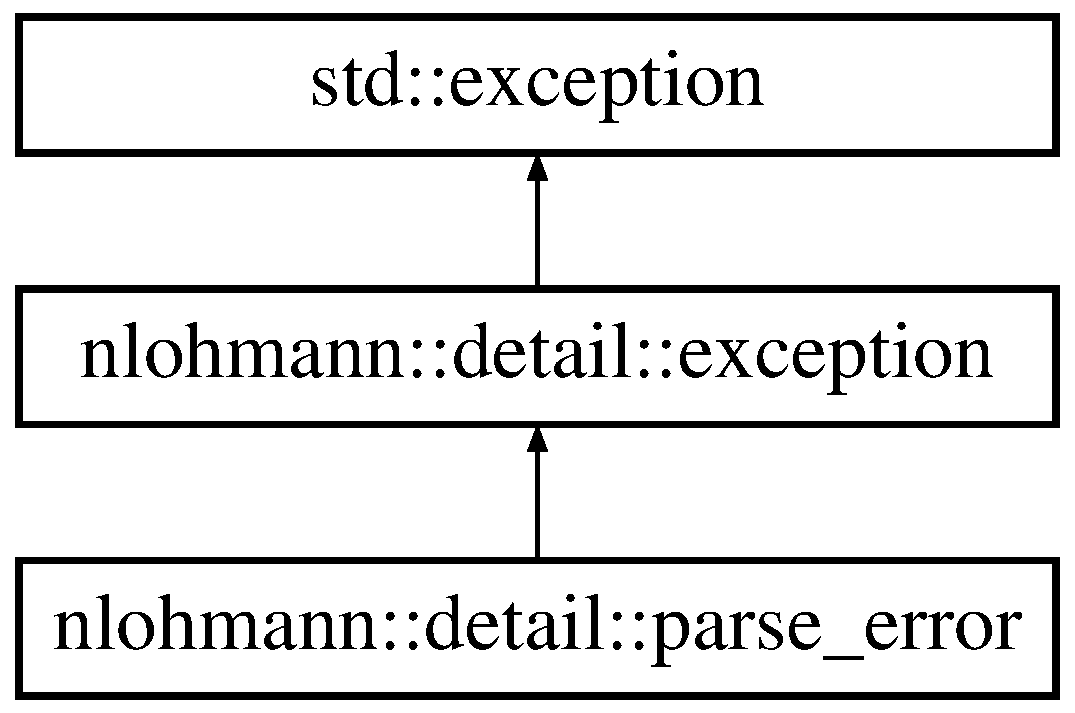
\includegraphics[height=3.000000cm]{d5/d1a/classnlohmann_1_1detail_1_1parse__error}
\end{center}
\end{figure}
\subsection*{Static Public Member Functions}
\begin{DoxyCompactItemize}
\item 
static \hyperlink{classnlohmann_1_1detail_1_1parse__error}{parse\+\_\+error} \hyperlink{classnlohmann_1_1detail_1_1parse__error_a53dd6b47379f42dbf3fe12500614adcb}{create} (int \hyperlink{classnlohmann_1_1detail_1_1exception_a0d4589a3fb54e81646d986c05efa3b9a}{id}, size\+\_\+t byte\+\_\+, const \hyperlink{namespacenlohmann_1_1detail_a90aa5ef615aa8305e9ea20d8a947980fab45cffe084dd3d20d928bee85e7b0f21}{std\+::string} \&what\+\_\+arg)
\begin{DoxyCompactList}\small\item\em create a parse error exception \end{DoxyCompactList}\end{DoxyCompactItemize}
\subsection*{Public Attributes}
\begin{DoxyCompactItemize}
\item 
const size\+\_\+t \hyperlink{classnlohmann_1_1detail_1_1parse__error_aa03a5254e185a08cc01502344f8b92fe}{byte}
\begin{DoxyCompactList}\small\item\em byte index of the parse error \end{DoxyCompactList}\end{DoxyCompactItemize}
\subsection*{Additional Inherited Members}


\subsection{Detailed Description}
exception indicating a parse error 

This excpetion is thrown by the library when a parse error occurs. Parse errors can occur during the deserialization of J\+S\+ON text as well as when using J\+S\+ON Patch.

Member {\itshape byte} holds the byte index of the last read character in the input file.

\begin{DoxyNote}{Note}
For an input with n bytes, 1 is the index of the first character and n+1 is the index of the terminating null byte or the end of file. This also holds true when reading a byte vector (C\+B\+OR or Message\+Pack).
\end{DoxyNote}
Exceptions have ids 1xx.

\tabulinesep=1mm
\begin{longtabu} spread 0pt [c]{*{3}{|X[-1]}|}
\hline
\rowcolor{\tableheadbgcolor}\textbf{ name / id }&\textbf{ example massage }&\textbf{ description  }\\\cline{1-3}
\endfirsthead
\hline
\endfoot
\hline
\rowcolor{\tableheadbgcolor}\textbf{ name / id }&\textbf{ example massage }&\textbf{ description  }\\\cline{1-3}
\endhead
json.\+exception.\+parse\+\_\+error.\+101 &parse error at 2\+: unexpected end of input; expected string literal &This error indicates a syntax error while deserializing a J\+S\+ON text. The error message describes that an unexpected token (character) was encountered, and the member {\itshape byte} indicates the error position. \\\cline{1-3}
json.\+exception.\+parse\+\_\+error.\+102 &parse error at 14\+: missing or wrong low surrogate &J\+S\+ON uses the {\ttfamily \textbackslash{}uxxxx} format to describe Unicode characters. Code points above above 0x\+F\+F\+FF are split into two {\ttfamily \textbackslash{}uxxxx} entries (\char`\"{}surrogate pairs\char`\"{}). This error indicates that the surrogate pair is incomplete or contains an invalid code point. \\\cline{1-3}
json.\+exception.\+parse\+\_\+error.\+103 &parse error\+: code points above 0x10\+F\+F\+FF are invalid &Unicode supports code points up to 0x10\+F\+F\+FF. Code points above 0x10\+F\+F\+FF are invalid. \\\cline{1-3}
json.\+exception.\+parse\+\_\+error.\+104 &parse error\+: J\+S\+ON patch must be an array of objects &\href{https://tools.ietf.org/html/rfc6902}{\tt R\+FC 6902} requires a J\+S\+ON Patch document to be a J\+S\+ON document that represents an array of objects. \\\cline{1-3}
json.\+exception.\+parse\+\_\+error.\+105 &parse error\+: operation must have string member \textquotesingle{}op\textquotesingle{} &An operation of a J\+S\+ON Patch document must contain exactly one \char`\"{}op\char`\"{} member, whose value indicates the operation to perform. Its value must be one of \char`\"{}add\char`\"{}, \char`\"{}remove\char`\"{}, \char`\"{}replace\char`\"{}, \char`\"{}move\char`\"{}, \char`\"{}copy\char`\"{}, or \char`\"{}test\char`\"{}; other values are errors. \\\cline{1-3}
json.\+exception.\+parse\+\_\+error.\+106 &parse error\+: array index \textquotesingle{}01\textquotesingle{} must not begin with \textquotesingle{}0\textquotesingle{} &An array index in a J\+S\+ON Pointer (\href{https://tools.ietf.org/html/rfc6901}{\tt R\+FC 6901}) may be {\ttfamily 0} or any number wihtout a leading {\ttfamily 0}. \\\cline{1-3}
json.\+exception.\+parse\+\_\+error.\+107 &parse error\+: J\+S\+ON pointer must be empty or begin with \textquotesingle{}/\textquotesingle{} -\/ was\+: \textquotesingle{}foo\textquotesingle{} &A J\+S\+ON Pointer must be a Unicode string containing a sequence of zero or more reference tokens, each prefixed by a {\ttfamily /} character. \\\cline{1-3}
json.\+exception.\+parse\+\_\+error.\+108 &parse error\+: escape character \textquotesingle{}$\sim$\textquotesingle{} must be followed with \textquotesingle{}0\textquotesingle{} or \textquotesingle{}1\textquotesingle{} &In a J\+S\+ON Pointer, only {\ttfamily $\sim$0} and {\ttfamily $\sim$1} are valid escape sequences. \\\cline{1-3}
json.\+exception.\+parse\+\_\+error.\+109 &parse error\+: array index \textquotesingle{}one\textquotesingle{} is not a number &A J\+S\+ON Pointer array index must be a number. \\\cline{1-3}
json.\+exception.\+parse\+\_\+error.\+110 &parse error at 1\+: cannot read 2 bytes from vector &When parsing C\+B\+OR or Message\+Pack, the byte vector ends before the complete value has been read. \\\cline{1-3}
json.\+exception.\+parse\+\_\+error.\+111 &parse error\+: bad input stream &Parsing C\+B\+OR or Message\+Pack from an input stream where the \href{http://en.cppreference.com/w/cpp/io/ios_base/iostate}{\tt {\ttfamily badbit} or {\ttfamily failbit}} is set. \\\cline{1-3}
json.\+exception.\+parse\+\_\+error.\+112 &parse error at 1\+: error reading C\+B\+OR; last byte\+: 0xf8 &Not all types of C\+B\+OR or Message\+Pack are supported. This exception occurs if an unsupported byte was read. \\\cline{1-3}
json.\+exception.\+parse\+\_\+error.\+113 &parse error at 2\+: expected a C\+B\+OR string; last byte\+: 0x98 &While parsing a map key, a value that is not a string has been read. \\\cline{1-3}
\end{longtabu}
\begin{DoxySince}{Since}
version 3.\+0.\+0 
\end{DoxySince}


\subsection{Member Function Documentation}
\mbox{\Hypertarget{classnlohmann_1_1detail_1_1parse__error_a53dd6b47379f42dbf3fe12500614adcb}\label{classnlohmann_1_1detail_1_1parse__error_a53dd6b47379f42dbf3fe12500614adcb}} 
\index{nlohmann\+::detail\+::parse\+\_\+error@{nlohmann\+::detail\+::parse\+\_\+error}!create@{create}}
\index{create@{create}!nlohmann\+::detail\+::parse\+\_\+error@{nlohmann\+::detail\+::parse\+\_\+error}}
\subsubsection{\texorpdfstring{create()}{create()}}
{\footnotesize\ttfamily static \hyperlink{classnlohmann_1_1detail_1_1parse__error}{parse\+\_\+error} nlohmann\+::detail\+::parse\+\_\+error\+::create (\begin{DoxyParamCaption}\item[{int}]{id,  }\item[{size\+\_\+t}]{byte\+\_\+,  }\item[{const \hyperlink{namespacenlohmann_1_1detail_a90aa5ef615aa8305e9ea20d8a947980fab45cffe084dd3d20d928bee85e7b0f21}{std\+::string} \&}]{what\+\_\+arg }\end{DoxyParamCaption})\hspace{0.3cm}{\ttfamily [inline]}, {\ttfamily [static]}}



create a parse error exception 


\begin{DoxyParams}[1]{Parameters}
\mbox{\tt in}  & {\em id} & the id of the exception \\
\hline
\mbox{\tt in}  & {\em byte\+\_\+} & the byte index where the error occured (or 0 if the position cannot be determined) \\
\hline
\mbox{\tt in}  & {\em what\+\_\+arg} & the explanatory string \\
\hline
\end{DoxyParams}
\begin{DoxyReturn}{Returns}
\hyperlink{classnlohmann_1_1detail_1_1parse__error}{parse\+\_\+error} object 
\end{DoxyReturn}


\subsection{Member Data Documentation}
\mbox{\Hypertarget{classnlohmann_1_1detail_1_1parse__error_aa03a5254e185a08cc01502344f8b92fe}\label{classnlohmann_1_1detail_1_1parse__error_aa03a5254e185a08cc01502344f8b92fe}} 
\index{nlohmann\+::detail\+::parse\+\_\+error@{nlohmann\+::detail\+::parse\+\_\+error}!byte@{byte}}
\index{byte@{byte}!nlohmann\+::detail\+::parse\+\_\+error@{nlohmann\+::detail\+::parse\+\_\+error}}
\subsubsection{\texorpdfstring{byte}{byte}}
{\footnotesize\ttfamily const size\+\_\+t nlohmann\+::detail\+::parse\+\_\+error\+::byte}



byte index of the parse error 

The byte index of the last read character in the input file.

\begin{DoxyNote}{Note}
For an input with n bytes, 1 is the index of the first character and n+1 is the index of the terminating null byte or the end of file. This also holds true when reading a byte vector (C\+B\+OR or Message\+Pack). 
\end{DoxyNote}


The documentation for this class was generated from the following file\+:\begin{DoxyCompactItemize}
\item 
/home/mutzi/progs/linux\+\_\+workspace/alexa-\/avs-\/prototype/src/include/nlohmann\+\_\+json.\+h\end{DoxyCompactItemize}

\hypertarget{structAVSJson_1_1PayloadPlaybackFailedParam}{}\section{A\+V\+S\+Json\+:\+:Payload\+Playback\+Failed\+Param Struct Reference}
\label{structAVSJson_1_1PayloadPlaybackFailedParam}\index{A\+V\+S\+Json\+::\+Payload\+Playback\+Failed\+Param@{A\+V\+S\+Json\+::\+Payload\+Playback\+Failed\+Param}}
\subsection*{Public Attributes}
\begin{DoxyCompactItemize}
\item 
\mbox{\Hypertarget{structAVSJson_1_1PayloadPlaybackFailedParam_a3f603f32f98f057205411db2cf56ded9}\label{structAVSJson_1_1PayloadPlaybackFailedParam_a3f603f32f98f057205411db2cf56ded9}} 
std\+::string {\bfseries token}
\item 
\mbox{\Hypertarget{structAVSJson_1_1PayloadPlaybackFailedParam_a7303b1ac14d549ca2fd7399b32a5a847}\label{structAVSJson_1_1PayloadPlaybackFailedParam_a7303b1ac14d549ca2fd7399b32a5a847}} 
std\+::string {\bfseries playback\+State\+\_\+token}
\item 
\mbox{\Hypertarget{structAVSJson_1_1PayloadPlaybackFailedParam_ac0ec827453cece0c09acb19570582ad1}\label{structAVSJson_1_1PayloadPlaybackFailedParam_ac0ec827453cece0c09acb19570582ad1}} 
std\+::string {\bfseries playback\+State\+\_\+offset}
\item 
\mbox{\Hypertarget{structAVSJson_1_1PayloadPlaybackFailedParam_aa0d01b525dd88b6e346c5e794283399a}\label{structAVSJson_1_1PayloadPlaybackFailedParam_aa0d01b525dd88b6e346c5e794283399a}} 
std\+::string {\bfseries playback\+State\+\_\+activity}
\item 
\mbox{\Hypertarget{structAVSJson_1_1PayloadPlaybackFailedParam_a33c6b6474d7219fa6e3ec0aae2877396}\label{structAVSJson_1_1PayloadPlaybackFailedParam_a33c6b6474d7219fa6e3ec0aae2877396}} 
std\+::string {\bfseries error\+\_\+type}
\item 
\mbox{\Hypertarget{structAVSJson_1_1PayloadPlaybackFailedParam_aeb11c1f814e512755adf89a169ebec6b}\label{structAVSJson_1_1PayloadPlaybackFailedParam_aeb11c1f814e512755adf89a169ebec6b}} 
std\+::string {\bfseries error\+\_\+message}
\end{DoxyCompactItemize}


The documentation for this struct was generated from the following file\+:\begin{DoxyCompactItemize}
\item 
/home/mutzi/progs/linux\+\_\+workspace/alexa-\/avs-\/prototype/src/include/jsonfactory.\+h\end{DoxyCompactItemize}

\hypertarget{structPlaybackQueue}{}\section{Playback\+Queue Struct Reference}
\label{structPlaybackQueue}\index{Playback\+Queue@{Playback\+Queue}}
\subsection*{Public Attributes}
\begin{DoxyCompactItemize}
\item 
\mbox{\Hypertarget{structPlaybackQueue_a5d5095ae9e62e6c38430841bf040dac7}\label{structPlaybackQueue_a5d5095ae9e62e6c38430841bf040dac7}} 
char $\ast$ {\bfseries mp3\+\_\+data}
\item 
\mbox{\Hypertarget{structPlaybackQueue_a1c65f5c767229a130f59f6e1bca5dee3}\label{structPlaybackQueue_a1c65f5c767229a130f59f6e1bca5dee3}} 
size\+\_\+t {\bfseries mp3\+\_\+size}
\item 
\mbox{\Hypertarget{structPlaybackQueue_a9b9438f6c78ce5cf5a9f2841a944e2f1}\label{structPlaybackQueue_a9b9438f6c78ce5cf5a9f2841a944e2f1}} 
std\+::string {\bfseries token}
\item 
\mbox{\Hypertarget{structPlaybackQueue_a169c296ea0dabce41d1e8f8a7afd0835}\label{structPlaybackQueue_a169c296ea0dabce41d1e8f8a7afd0835}} 
long {\bfseries offset\+In\+Milliseconds}
\end{DoxyCompactItemize}


The documentation for this struct was generated from the following file\+:\begin{DoxyCompactItemize}
\item 
/home/mutzi/progs/linux\+\_\+workspace/alexa-\/avs-\/prototype/src/include/avsplaybackcontroller.\+h\end{DoxyCompactItemize}

\hypertarget{structAVSJson_1_1PlaybackState}{}\section{A\+V\+S\+Json\+:\+:Playback\+State Struct Reference}
\label{structAVSJson_1_1PlaybackState}\index{A\+V\+S\+Json\+::\+Playback\+State@{A\+V\+S\+Json\+::\+Playback\+State}}
\subsection*{Public Attributes}
\begin{DoxyCompactItemize}
\item 
\mbox{\Hypertarget{structAVSJson_1_1PlaybackState_ac1305454c79dad90ab57c1e9a7ce9a58}\label{structAVSJson_1_1PlaybackState_ac1305454c79dad90ab57c1e9a7ce9a58}} 
std\+::string {\bfseries token}
\item 
\mbox{\Hypertarget{structAVSJson_1_1PlaybackState_a55fc2d8f8658eb25e8747efd24ed3de1}\label{structAVSJson_1_1PlaybackState_a55fc2d8f8658eb25e8747efd24ed3de1}} 
long {\bfseries offset\+In\+Milliseconds}
\item 
\mbox{\Hypertarget{structAVSJson_1_1PlaybackState_a5ded107980d738b144d6233c67a03e5c}\label{structAVSJson_1_1PlaybackState_a5ded107980d738b144d6233c67a03e5c}} 
std\+::string {\bfseries player\+Activity}
\end{DoxyCompactItemize}


The documentation for this struct was generated from the following file\+:\begin{DoxyCompactItemize}
\item 
/home/mutzi/progs/linux\+\_\+workspace/alexa-\/avs-\/prototype/src/include/jsonfactory.\+h\end{DoxyCompactItemize}

\hypertarget{structnlohmann_1_1detail_1_1priority__tag}{}\section{nlohmann\+:\+:detail\+:\+:priority\+\_\+tag$<$ N $>$ Struct Template Reference}
\label{structnlohmann_1_1detail_1_1priority__tag}\index{nlohmann\+::detail\+::priority\+\_\+tag$<$ N $>$@{nlohmann\+::detail\+::priority\+\_\+tag$<$ N $>$}}


The documentation for this struct was generated from the following file\+:\begin{DoxyCompactItemize}
\item 
/home/mutzi/progs/linux\+\_\+workspace/alexa-\/avs-\/prototype/src/include/nlohmann\+\_\+json.\+h\end{DoxyCompactItemize}

\hypertarget{structnlohmann_1_1detail_1_1priority__tag_3_010_01_4}{}\section{nlohmann\+:\+:detail\+:\+:priority\+\_\+tag$<$ 0 $>$ Struct Template Reference}
\label{structnlohmann_1_1detail_1_1priority__tag_3_010_01_4}\index{nlohmann\+::detail\+::priority\+\_\+tag$<$ 0 $>$@{nlohmann\+::detail\+::priority\+\_\+tag$<$ 0 $>$}}


The documentation for this struct was generated from the following file\+:\begin{DoxyCompactItemize}
\item 
/home/mutzi/progs/linux\+\_\+workspace/alexa-\/avs-\/prototype/src/include/nlohmann\+\_\+json.\+h\end{DoxyCompactItemize}

\hypertarget{structAVSJson_1_1RecognizeState}{}\section{A\+V\+S\+Json\+:\+:Recognize\+State Struct Reference}
\label{structAVSJson_1_1RecognizeState}\index{A\+V\+S\+Json\+::\+Recognize\+State@{A\+V\+S\+Json\+::\+Recognize\+State}}
\subsection*{Public Attributes}
\begin{DoxyCompactItemize}
\item 
\mbox{\Hypertarget{structAVSJson_1_1RecognizeState_ad9a2cf658755a87fb9cf64e697a34a0d}\label{structAVSJson_1_1RecognizeState_ad9a2cf658755a87fb9cf64e697a34a0d}} 
std\+::string {\bfseries wakeword}
\end{DoxyCompactItemize}


The documentation for this struct was generated from the following file\+:\begin{DoxyCompactItemize}
\item 
/home/mutzi/progs/linux\+\_\+workspace/alexa-\/avs-\/prototype/src/include/jsonfactory.\+h\end{DoxyCompactItemize}

\hypertarget{classThread_1_1Runnable}{}\section{Thread\+:\+:Runnable Class Reference}
\label{classThread_1_1Runnable}\index{Thread\+::\+Runnable@{Thread\+::\+Runnable}}
Inheritance diagram for Thread\+:\+:Runnable\+:\begin{figure}[H]
\begin{center}
\leavevmode
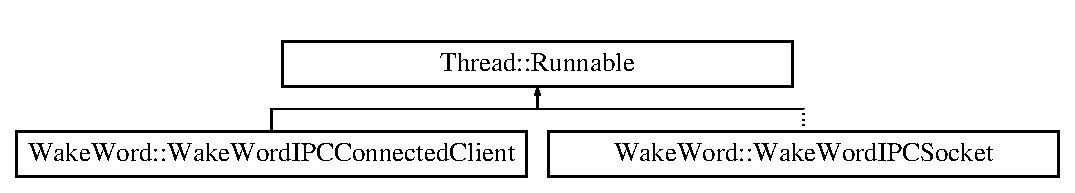
\includegraphics[height=2.000000cm]{df/d39/classThread_1_1Runnable}
\end{center}
\end{figure}
\subsection*{Public Member Functions}
\begin{DoxyCompactItemize}
\item 
\mbox{\Hypertarget{classThread_1_1Runnable_a334fde08ab60a6f468f587751370b5a7}\label{classThread_1_1Runnable_a334fde08ab60a6f468f587751370b5a7}} 
virtual void {\bfseries run} ()=0
\end{DoxyCompactItemize}


The documentation for this class was generated from the following file\+:\begin{DoxyCompactItemize}
\item 
/home/mutzi/progs/linux\+\_\+workspace/alexa-\/avs-\/prototype/src/include/Runnable.\+h\end{DoxyCompactItemize}

\hypertarget{classNetwork_1_1NetSocket_1_1ServerSocket}{}\section{Network\+:\+:Net\+Socket\+:\+:Server\+Socket Class Reference}
\label{classNetwork_1_1NetSocket_1_1ServerSocket}\index{Network\+::\+Net\+Socket\+::\+Server\+Socket@{Network\+::\+Net\+Socket\+::\+Server\+Socket}}
\subsection*{Public Member Functions}
\begin{DoxyCompactItemize}
\item 
\mbox{\Hypertarget{classNetwork_1_1NetSocket_1_1ServerSocket_a50d9085b678fcd32f0ebfbcbcd4198cc}\label{classNetwork_1_1NetSocket_1_1ServerSocket_a50d9085b678fcd32f0ebfbcbcd4198cc}} 
{\bfseries Server\+Socket} (int port\+Number)
\item 
\mbox{\Hypertarget{classNetwork_1_1NetSocket_1_1ServerSocket_a4d2a3ecda6b18f9eeadf4d21f3f8bc06}\label{classNetwork_1_1NetSocket_1_1ServerSocket_a4d2a3ecda6b18f9eeadf4d21f3f8bc06}} 
int {\bfseries socket\+Accept} ()  throw ( std\+::exception )
\item 
\mbox{\Hypertarget{classNetwork_1_1NetSocket_1_1ServerSocket_a2b80f507eeee6c22889e63eb164429e5}\label{classNetwork_1_1NetSocket_1_1ServerSocket_a2b80f507eeee6c22889e63eb164429e5}} 
void {\bfseries destroy\+\_\+socket} (int client\+\_\+socket)
\item 
\mbox{\Hypertarget{classNetwork_1_1NetSocket_1_1ServerSocket_a98ab276ee61212119614f789d167ef7b}\label{classNetwork_1_1NetSocket_1_1ServerSocket_a98ab276ee61212119614f789d167ef7b}} 
void {\bfseries destroy\+\_\+server} ()
\end{DoxyCompactItemize}


The documentation for this class was generated from the following files\+:\begin{DoxyCompactItemize}
\item 
/home/mutzi/progs/linux\+\_\+workspace/alexa-\/avs-\/prototype/src/include/serversocket.\+h\item 
/home/mutzi/progs/linux\+\_\+workspace/alexa-\/avs-\/prototype/src/serversocket.\+cpp\end{DoxyCompactItemize}

\hypertarget{structAVSJson_1_1SpeechState}{}\section{A\+V\+S\+Json\+:\+:Speech\+State Struct Reference}
\label{structAVSJson_1_1SpeechState}\index{A\+V\+S\+Json\+::\+Speech\+State@{A\+V\+S\+Json\+::\+Speech\+State}}
\subsection*{Public Attributes}
\begin{DoxyCompactItemize}
\item 
\mbox{\Hypertarget{structAVSJson_1_1SpeechState_ad7804b99a11d58480642eb6771a77e94}\label{structAVSJson_1_1SpeechState_ad7804b99a11d58480642eb6771a77e94}} 
std\+::string {\bfseries token}
\item 
\mbox{\Hypertarget{structAVSJson_1_1SpeechState_a343954dfa5bdb1af1f9939b279709afe}\label{structAVSJson_1_1SpeechState_a343954dfa5bdb1af1f9939b279709afe}} 
long {\bfseries offset\+In\+Milliseconds}
\item 
\mbox{\Hypertarget{structAVSJson_1_1SpeechState_a6f0cbc9d555e97028f9bfbd0c12f8041}\label{structAVSJson_1_1SpeechState_a6f0cbc9d555e97028f9bfbd0c12f8041}} 
std\+::string {\bfseries player\+Activity}
\end{DoxyCompactItemize}


The documentation for this struct was generated from the following file\+:\begin{DoxyCompactItemize}
\item 
/home/mutzi/progs/linux\+\_\+workspace/alexa-\/avs-\/prototype/src/include/jsonfactory.\+h\end{DoxyCompactItemize}

\hypertarget{structnlohmann_1_1detail_1_1static__const}{}\section{nlohmann\+:\+:detail\+:\+:static\+\_\+const$<$ T $>$ Struct Template Reference}
\label{structnlohmann_1_1detail_1_1static__const}\index{nlohmann\+::detail\+::static\+\_\+const$<$ T $>$@{nlohmann\+::detail\+::static\+\_\+const$<$ T $>$}}
\subsection*{Static Public Attributes}
\begin{DoxyCompactItemize}
\item 
\mbox{\Hypertarget{structnlohmann_1_1detail_1_1static__const_a6bb7ab2ddd6abc41fb4ffb7c6dfa237e}\label{structnlohmann_1_1detail_1_1static__const_a6bb7ab2ddd6abc41fb4ffb7c6dfa237e}} 
static constexpr T {\bfseries value} \{\}
\end{DoxyCompactItemize}


The documentation for this struct was generated from the following file\+:\begin{DoxyCompactItemize}
\item 
/home/mutzi/progs/linux\+\_\+workspace/alexa-\/avs-\/prototype/src/include/nlohmann\+\_\+json.\+h\end{DoxyCompactItemize}

\hypertarget{structNetwork_1_1HTTP2_1_1StreamQueueData}{}\section{Network\+:\+:H\+T\+T\+P2\+:\+:Stream\+Queue\+Data Struct Reference}
\label{structNetwork_1_1HTTP2_1_1StreamQueueData}\index{Network\+::\+H\+T\+T\+P2\+::\+Stream\+Queue\+Data@{Network\+::\+H\+T\+T\+P2\+::\+Stream\+Queue\+Data}}
\subsection*{Public Attributes}
\begin{DoxyCompactItemize}
\item 
\mbox{\Hypertarget{structNetwork_1_1HTTP2_1_1StreamQueueData_a1c68711a4f22b732630accd4f574efc0}\label{structNetwork_1_1HTTP2_1_1StreamQueueData_a1c68711a4f22b732630accd4f574efc0}} 
nghttp2\+\_\+nv $\ast$ {\bfseries header\+\_\+data}
\item 
\mbox{\Hypertarget{structNetwork_1_1HTTP2_1_1StreamQueueData_a7c3e7909a7c09c3ff37664a5f0d8c74a}\label{structNetwork_1_1HTTP2_1_1StreamQueueData_a7c3e7909a7c09c3ff37664a5f0d8c74a}} 
char $\ast$ {\bfseries source\+\_\+data}
\item 
\mbox{\Hypertarget{structNetwork_1_1HTTP2_1_1StreamQueueData_acc80b01bfd60041e2e70d25fb32261b0}\label{structNetwork_1_1HTTP2_1_1StreamQueueData_acc80b01bfd60041e2e70d25fb32261b0}} 
size\+\_\+t {\bfseries header\+\_\+len}
\item 
\mbox{\Hypertarget{structNetwork_1_1HTTP2_1_1StreamQueueData_a9ee58c0936ac2bb080c6aab2362f2541}\label{structNetwork_1_1HTTP2_1_1StreamQueueData_a9ee58c0936ac2bb080c6aab2362f2541}} 
size\+\_\+t {\bfseries source\+\_\+len}
\end{DoxyCompactItemize}


The documentation for this struct was generated from the following file\+:\begin{DoxyCompactItemize}
\item 
/home/mutzi/progs/linux\+\_\+workspace/alexa-\/avs-\/prototype/src/include/nghttp2multiplexhandler.\+h\end{DoxyCompactItemize}

\hypertarget{structnlohmann_1_1basic__json_1_1lexer_1_1strtonum}{}\section{nlohmann\+:\+:basic\+\_\+json$<$ Object\+Type, Array\+Type, String\+Type, Boolean\+Type, Number\+Integer\+Type, Number\+Unsigned\+Type, Number\+Float\+Type, Allocator\+Type, J\+S\+O\+N\+Serializer $>$\+:\+:lexer\+:\+:strtonum Struct Reference}
\label{structnlohmann_1_1basic__json_1_1lexer_1_1strtonum}\index{nlohmann\+::basic\+\_\+json$<$ Object\+Type, Array\+Type, String\+Type, Boolean\+Type, Number\+Integer\+Type, Number\+Unsigned\+Type, Number\+Float\+Type, Allocator\+Type, J\+S\+O\+N\+Serializer $>$\+::lexer\+::strtonum@{nlohmann\+::basic\+\_\+json$<$ Object\+Type, Array\+Type, String\+Type, Boolean\+Type, Number\+Integer\+Type, Number\+Unsigned\+Type, Number\+Float\+Type, Allocator\+Type, J\+S\+O\+N\+Serializer $>$\+::lexer\+::strtonum}}


parse string into a built-\/in arithmetic type as if the current locale is P\+O\+S\+IX.  




{\ttfamily \#include $<$nlohmann\+\_\+json.\+h$>$}

\subsection*{Public Member Functions}
\begin{DoxyCompactItemize}
\item 
\mbox{\Hypertarget{structnlohmann_1_1basic__json_1_1lexer_1_1strtonum_ae065098e24b08ea79a359950190006d8}\label{structnlohmann_1_1basic__json_1_1lexer_1_1strtonum_ae065098e24b08ea79a359950190006d8}} 
{\bfseries strtonum} (const char $\ast$start, const char $\ast$\hyperlink{classnlohmann_1_1basic__json_a13e032a02a7fd8a93fdddc2fcbc4763c}{end})
\item 
{\footnotesize template$<$typename T , typename  = typename std\+::enable\+\_\+if$<$std\+::is\+\_\+arithmetic$<$\+T$>$\+::value$>$\+::type$>$ }\\bool \hyperlink{structnlohmann_1_1basic__json_1_1lexer_1_1strtonum_af1b3dc99a67a854750437a60a22f4989}{to} (T \&val) const
\end{DoxyCompactItemize}


\subsection{Detailed Description}
\subsubsection*{template$<$template$<$ typename U, typename V, typename... Args $>$ class Object\+Type = std\+::map, template$<$ typename U, typename... Args $>$ class Array\+Type = std\+::vector, class String\+Type = std\+::string, class Boolean\+Type = bool, class Number\+Integer\+Type = std\+::int64\+\_\+t, class Number\+Unsigned\+Type = std\+::uint64\+\_\+t, class Number\+Float\+Type = double, template$<$ typename U $>$ class Allocator\+Type = std\+::allocator, template$<$ typename T, typename S\+F\+I\+N\+A\+E=void $>$ class J\+S\+O\+N\+Serializer = adl\+\_\+serializer$>$\newline
struct nlohmann\+::basic\+\_\+json$<$ Object\+Type, Array\+Type, String\+Type, Boolean\+Type, Number\+Integer\+Type, Number\+Unsigned\+Type, Number\+Float\+Type, Allocator\+Type, J\+S\+O\+N\+Serializer $>$\+::lexer\+::strtonum}

parse string into a built-\/in arithmetic type as if the current locale is P\+O\+S\+IX. 

\begin{DoxyNote}{Note}
in floating-\/point case strtod may parse past the token\textquotesingle{}s end -\/ this is not an error

any leading blanks are not handled 
\end{DoxyNote}


\subsection{Member Function Documentation}
\mbox{\Hypertarget{structnlohmann_1_1basic__json_1_1lexer_1_1strtonum_af1b3dc99a67a854750437a60a22f4989}\label{structnlohmann_1_1basic__json_1_1lexer_1_1strtonum_af1b3dc99a67a854750437a60a22f4989}} 
\index{nlohmann\+::basic\+\_\+json\+::lexer\+::strtonum@{nlohmann\+::basic\+\_\+json\+::lexer\+::strtonum}!to@{to}}
\index{to@{to}!nlohmann\+::basic\+\_\+json\+::lexer\+::strtonum@{nlohmann\+::basic\+\_\+json\+::lexer\+::strtonum}}
\subsubsection{\texorpdfstring{to()}{to()}}
{\footnotesize\ttfamily template$<$template$<$ typename U, typename V, typename... Args $>$ class Object\+Type = std\+::map, template$<$ typename U, typename... Args $>$ class Array\+Type = std\+::vector, class String\+Type  = std\+::string, class Boolean\+Type  = bool, class Number\+Integer\+Type  = std\+::int64\+\_\+t, class Number\+Unsigned\+Type  = std\+::uint64\+\_\+t, class Number\+Float\+Type  = double, template$<$ typename U $>$ class Allocator\+Type = std\+::allocator, template$<$ typename T, typename S\+F\+I\+N\+A\+E=void $>$ class J\+S\+O\+N\+Serializer = adl\+\_\+serializer$>$ \\
template$<$typename T , typename  = typename std\+::enable\+\_\+if$<$std\+::is\+\_\+arithmetic$<$\+T$>$\+::value$>$\+::type$>$ \\
bool \hyperlink{classnlohmann_1_1basic__json}{nlohmann\+::basic\+\_\+json}$<$ Object\+Type, Array\+Type, String\+Type, Boolean\+Type, Number\+Integer\+Type, Number\+Unsigned\+Type, Number\+Float\+Type, Allocator\+Type, J\+S\+O\+N\+Serializer $>$\+::lexer\+::strtonum\+::to (\begin{DoxyParamCaption}\item[{T \&}]{val }\end{DoxyParamCaption}) const\hspace{0.3cm}{\ttfamily [inline]}}

\begin{DoxyReturn}{Returns}
true iff parsed successfully as number of type T
\end{DoxyReturn}

\begin{DoxyParams}[1]{Parameters}
\mbox{\tt in,out}  & {\em val} & shall contain parsed value, or undefined value if could not parse \\
\hline
\end{DoxyParams}


The documentation for this struct was generated from the following file\+:\begin{DoxyCompactItemize}
\item 
/home/mutzi/progs/linux\+\_\+workspace/alexa-\/avs-\/prototype/src/include/nlohmann\+\_\+json.\+h\end{DoxyCompactItemize}

\hypertarget{structAVSJson_1_1SynchronizeStateEvent}{}\section{A\+V\+S\+Json\+:\+:Synchronize\+State\+Event Struct Reference}
\label{structAVSJson_1_1SynchronizeStateEvent}\index{A\+V\+S\+Json\+::\+Synchronize\+State\+Event@{A\+V\+S\+Json\+::\+Synchronize\+State\+Event}}
\subsection*{Public Attributes}
\begin{DoxyCompactItemize}
\item 
\mbox{\Hypertarget{structAVSJson_1_1SynchronizeStateEvent_affbc0de5b8ca8702b6ebae6b5c28dd64}\label{structAVSJson_1_1SynchronizeStateEvent_affbc0de5b8ca8702b6ebae6b5c28dd64}} 
\hyperlink{structAVSJson_1_1AlertsState}{Alerts\+State} $\ast$ {\bfseries alerts\+State}
\item 
\mbox{\Hypertarget{structAVSJson_1_1SynchronizeStateEvent_ace9dfc7c6158e171d1320b1a925dbfb3}\label{structAVSJson_1_1SynchronizeStateEvent_ace9dfc7c6158e171d1320b1a925dbfb3}} 
\hyperlink{structAVSJson_1_1PlaybackState}{Playback\+State} $\ast$ {\bfseries playback\+State}
\item 
\mbox{\Hypertarget{structAVSJson_1_1SynchronizeStateEvent_a9e6f85d95986947ea7d17fc3d99f0313}\label{structAVSJson_1_1SynchronizeStateEvent_a9e6f85d95986947ea7d17fc3d99f0313}} 
\hyperlink{structAVSJson_1_1VolumeState}{Volume\+State} $\ast$ {\bfseries volume\+State}
\item 
\mbox{\Hypertarget{structAVSJson_1_1SynchronizeStateEvent_a4a0391a93040e74c668307f402d70946}\label{structAVSJson_1_1SynchronizeStateEvent_a4a0391a93040e74c668307f402d70946}} 
\hyperlink{structAVSJson_1_1SpeechState}{Speech\+State} $\ast$ {\bfseries speech\+State}
\item 
\mbox{\Hypertarget{structAVSJson_1_1SynchronizeStateEvent_a375c547e70480e11becfb7b8165bfd7a}\label{structAVSJson_1_1SynchronizeStateEvent_a375c547e70480e11becfb7b8165bfd7a}} 
\hyperlink{structAVSJson_1_1RecognizeState}{Recognize\+State} $\ast$ {\bfseries recognize\+State}
\item 
\mbox{\Hypertarget{structAVSJson_1_1SynchronizeStateEvent_a48a80e6b79202e9be6e4e8ce87073566}\label{structAVSJson_1_1SynchronizeStateEvent_a48a80e6b79202e9be6e4e8ce87073566}} 
std\+::string {\bfseries message\+Id}
\end{DoxyCompactItemize}


The documentation for this struct was generated from the following file\+:\begin{DoxyCompactItemize}
\item 
/home/mutzi/progs/linux\+\_\+workspace/alexa-\/avs-\/prototype/src/include/jsonfactory.\+h\end{DoxyCompactItemize}

\hypertarget{structnlohmann_1_1detail_1_1to__json__fn}{}\section{nlohmann\+:\+:detail\+:\+:to\+\_\+json\+\_\+fn Struct Reference}
\label{structnlohmann_1_1detail_1_1to__json__fn}\index{nlohmann\+::detail\+::to\+\_\+json\+\_\+fn@{nlohmann\+::detail\+::to\+\_\+json\+\_\+fn}}
\subsection*{Public Member Functions}
\begin{DoxyCompactItemize}
\item 
\mbox{\Hypertarget{structnlohmann_1_1detail_1_1to__json__fn_ac63f82d3eed085522f1cbe99a521a4d4}\label{structnlohmann_1_1detail_1_1to__json__fn_ac63f82d3eed085522f1cbe99a521a4d4}} 
{\footnotesize template$<$typename Basic\+Json\+Type , typename T $>$ }\\void {\bfseries operator()} (Basic\+Json\+Type \&j, T \&\&val) const noexcept(noexcept(std\+::declval$<$ \hyperlink{structnlohmann_1_1detail_1_1to__json__fn}{to\+\_\+json\+\_\+fn} $>$().call(j, std\+::forward$<$ T $>$(val), \hyperlink{structnlohmann_1_1detail_1_1priority__tag}{priority\+\_\+tag}$<$ 1 $>$ \{\})))
\end{DoxyCompactItemize}


The documentation for this struct was generated from the following file\+:\begin{DoxyCompactItemize}
\item 
/home/mutzi/progs/linux\+\_\+workspace/alexa-\/avs-\/prototype/src/include/nlohmann\+\_\+json.\+h\end{DoxyCompactItemize}

\hypertarget{classnlohmann_1_1detail_1_1type__error}{}\section{nlohmann\+:\+:detail\+:\+:type\+\_\+error Class Reference}
\label{classnlohmann_1_1detail_1_1type__error}\index{nlohmann\+::detail\+::type\+\_\+error@{nlohmann\+::detail\+::type\+\_\+error}}


exception indicating executing a member function with a wrong type  




{\ttfamily \#include $<$nlohmann\+\_\+json.\+h$>$}

Inheritance diagram for nlohmann\+:\+:detail\+:\+:type\+\_\+error\+:\begin{figure}[H]
\begin{center}
\leavevmode
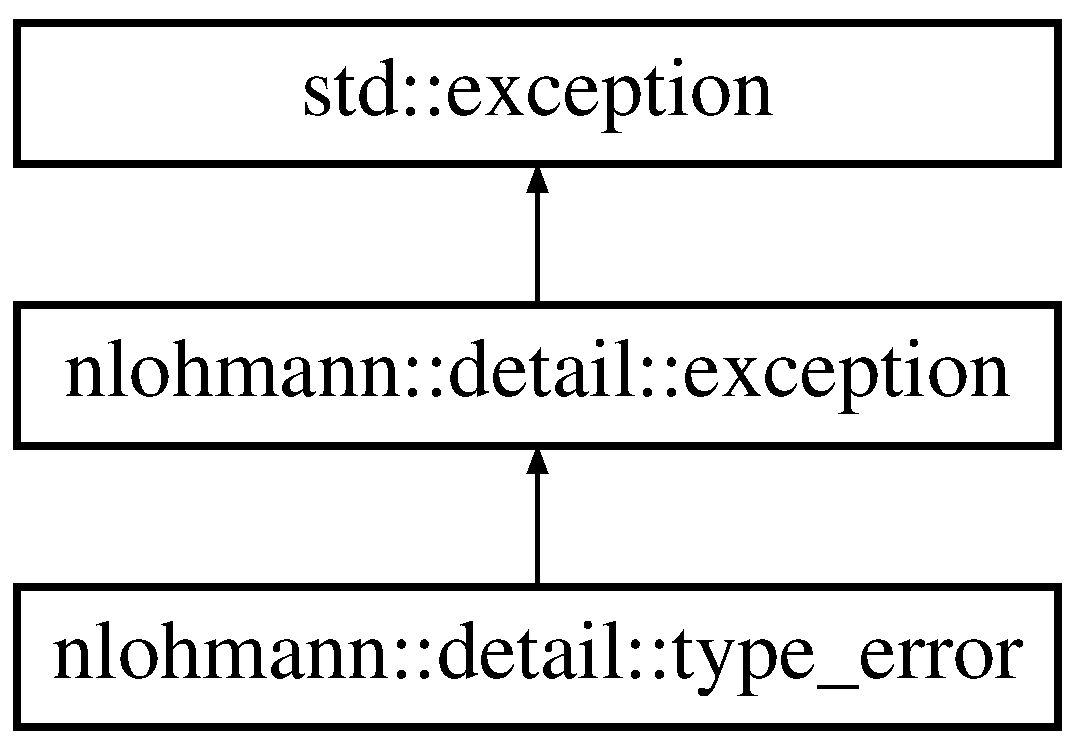
\includegraphics[height=3.000000cm]{da/d1c/classnlohmann_1_1detail_1_1type__error}
\end{center}
\end{figure}
\subsection*{Static Public Member Functions}
\begin{DoxyCompactItemize}
\item 
\mbox{\Hypertarget{classnlohmann_1_1detail_1_1type__error_a7f0db33eea838b258ee08c488a74b9ed}\label{classnlohmann_1_1detail_1_1type__error_a7f0db33eea838b258ee08c488a74b9ed}} 
static \hyperlink{classnlohmann_1_1detail_1_1type__error}{type\+\_\+error} {\bfseries create} (int \hyperlink{classnlohmann_1_1detail_1_1exception_a0d4589a3fb54e81646d986c05efa3b9a}{id}, const \hyperlink{namespacenlohmann_1_1detail_a90aa5ef615aa8305e9ea20d8a947980fab45cffe084dd3d20d928bee85e7b0f21}{std\+::string} \&what\+\_\+arg)
\end{DoxyCompactItemize}
\subsection*{Additional Inherited Members}


\subsection{Detailed Description}
exception indicating executing a member function with a wrong type 

Exceptions have ids 3xx.

\tabulinesep=1mm
\begin{longtabu} spread 0pt [c]{*{3}{|X[-1]}|}
\hline
\rowcolor{\tableheadbgcolor}\textbf{ name / id }&\textbf{ example massage }&\textbf{ description  }\\\cline{1-3}
\endfirsthead
\hline
\endfoot
\hline
\rowcolor{\tableheadbgcolor}\textbf{ name / id }&\textbf{ example massage }&\textbf{ description  }\\\cline{1-3}
\endhead
json.\+exception.\+type\+\_\+error.\+301 &cannot create object from initializer list &To create an object from an initializer list, the initializer list must consist only of a list of pairs whose first element is a string. When this constraint is violated, an array is created instead. \\\cline{1-3}
json.\+exception.\+type\+\_\+error.\+302 &type must be object, but is array &During implicit or explicit value conversion, the J\+S\+ON type must be compatible to the target type. For instance, a J\+S\+ON string can only be converted into string types, but not into numbers or boolean types. \\\cline{1-3}
json.\+exception.\+type\+\_\+error.\+303 &incompatible Reference\+Type for get\+\_\+ref, actual type is object &To retrieve a reference to a value stored in a \hyperlink{classnlohmann_1_1basic__json}{basic\+\_\+json} object with get\+\_\+ref, the type of the reference must match the value type. For instance, for a J\+S\+ON array, the {\itshape Reference\+Type} must be array\+\_\+t\&. \\\cline{1-3}
json.\+exception.\+type\+\_\+error.\+304 &cannot use at() with string &The at() member functions can only be executed for certain J\+S\+ON types. \\\cline{1-3}
json.\+exception.\+type\+\_\+error.\+305 &cannot use operator\mbox{[}\mbox{]} with string &The operator\mbox{[}\mbox{]} member functions can only be executed for certain J\+S\+ON types. \\\cline{1-3}
json.\+exception.\+type\+\_\+error.\+306 &cannot use value() with string &The value() member functions can only be executed for certain J\+S\+ON types. \\\cline{1-3}
json.\+exception.\+type\+\_\+error.\+307 &cannot use erase() with string &The erase() member functions can only be executed for certain J\+S\+ON types. \\\cline{1-3}
json.\+exception.\+type\+\_\+error.\+308 &cannot use push\+\_\+back() with string &The push\+\_\+back() and operator+= member functions can only be executed for certain J\+S\+ON types. \\\cline{1-3}
json.\+exception.\+type\+\_\+error.\+309 &cannot use insert() with &The insert() member functions can only be executed for certain J\+S\+ON types. \\\cline{1-3}
json.\+exception.\+type\+\_\+error.\+310 &cannot use swap() with number &The swap() member functions can only be executed for certain J\+S\+ON types. \\\cline{1-3}
json.\+exception.\+type\+\_\+error.\+311 &cannot use emplace\+\_\+back() with string &The emplace\+\_\+back() member function can only be executed for certain J\+S\+ON types. \\\cline{1-3}
json.\+exception.\+type\+\_\+error.\+313 &invalid value to unflatten &The unflatten function converts an object whose keys are J\+S\+ON Pointers back into an arbitrary nested J\+S\+ON value. The J\+S\+ON Pointers must not overlap, because then the resulting value would not be well defined. \\\cline{1-3}
json.\+exception.\+type\+\_\+error.\+314 &only objects can be unflattened &The unflatten function only works for an object whose keys are J\+S\+ON Pointers. \\\cline{1-3}
json.\+exception.\+type\+\_\+error.\+315 &values in object must be primitive &The unflatten function only works for an object whose keys are J\+S\+ON Pointers and whose values are primitive. \\\cline{1-3}
\end{longtabu}
\begin{DoxySince}{Since}
version 3.\+0.\+0 
\end{DoxySince}


The documentation for this class was generated from the following file\+:\begin{DoxyCompactItemize}
\item 
/home/mutzi/progs/linux\+\_\+workspace/alexa-\/avs-\/prototype/src/include/nlohmann\+\_\+json.\+h\end{DoxyCompactItemize}

\hypertarget{structAVSJson_1_1VolumeState}{}\section{A\+V\+S\+Json\+:\+:Volume\+State Struct Reference}
\label{structAVSJson_1_1VolumeState}\index{A\+V\+S\+Json\+::\+Volume\+State@{A\+V\+S\+Json\+::\+Volume\+State}}
\subsection*{Public Attributes}
\begin{DoxyCompactItemize}
\item 
\mbox{\Hypertarget{structAVSJson_1_1VolumeState_a9848bea24376afa8cd22606e1bd6407f}\label{structAVSJson_1_1VolumeState_a9848bea24376afa8cd22606e1bd6407f}} 
long {\bfseries volume}
\item 
\mbox{\Hypertarget{structAVSJson_1_1VolumeState_aaa620eb455be6074119fde9244d73dd1}\label{structAVSJson_1_1VolumeState_aaa620eb455be6074119fde9244d73dd1}} 
std\+::string {\bfseries muted}
\end{DoxyCompactItemize}


The documentation for this struct was generated from the following file\+:\begin{DoxyCompactItemize}
\item 
/home/mutzi/progs/linux\+\_\+workspace/alexa-\/avs-\/prototype/src/include/jsonfactory.\+h\end{DoxyCompactItemize}

\hypertarget{classWakeWord_1_1WakeWordDetectedHandler}{}\section{Wake\+Word\+:\+:Wake\+Word\+Detected\+Handler Class Reference}
\label{classWakeWord_1_1WakeWordDetectedHandler}\index{Wake\+Word\+::\+Wake\+Word\+Detected\+Handler@{Wake\+Word\+::\+Wake\+Word\+Detected\+Handler}}
Inheritance diagram for Wake\+Word\+:\+:Wake\+Word\+Detected\+Handler\+:\begin{figure}[H]
\begin{center}
\leavevmode
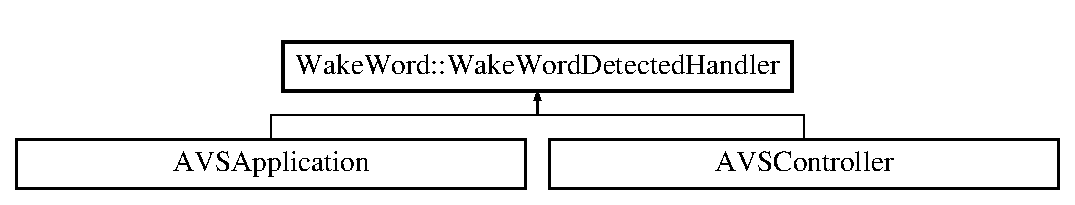
\includegraphics[height=2.000000cm]{d2/d12/classWakeWord_1_1WakeWordDetectedHandler}
\end{center}
\end{figure}
\subsection*{Public Member Functions}
\begin{DoxyCompactItemize}
\item 
\mbox{\Hypertarget{classWakeWord_1_1WakeWordDetectedHandler_a85d0040609d8e47367dd1fdac15fa462}\label{classWakeWord_1_1WakeWordDetectedHandler_a85d0040609d8e47367dd1fdac15fa462}} 
virtual void {\bfseries on\+Wake\+Word\+Detected} ()=0
\end{DoxyCompactItemize}


The documentation for this class was generated from the following file\+:\begin{DoxyCompactItemize}
\item 
/home/mutzi/progs/linux\+\_\+workspace/alexa-\/avs-\/prototype/src/include/wakeworddetectedhandler.\+h\end{DoxyCompactItemize}

\hypertarget{classWakeWord_1_1WakeWordIPC}{}\section{Wake\+Word\+:\+:Wake\+Word\+I\+PC Class Reference}
\label{classWakeWord_1_1WakeWordIPC}\index{Wake\+Word\+::\+Wake\+Word\+I\+PC@{Wake\+Word\+::\+Wake\+Word\+I\+PC}}
Inheritance diagram for Wake\+Word\+:\+:Wake\+Word\+I\+PC\+:\begin{figure}[H]
\begin{center}
\leavevmode
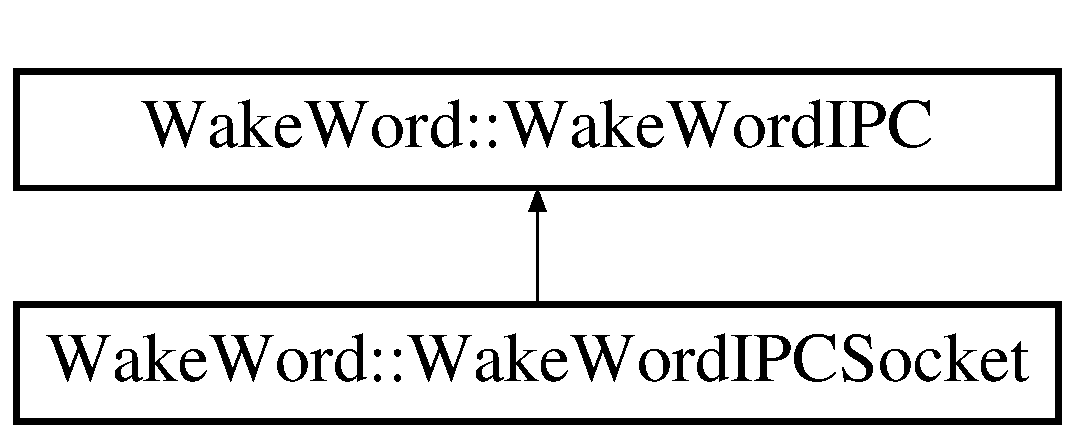
\includegraphics[height=2.000000cm]{df/d0a/classWakeWord_1_1WakeWordIPC}
\end{center}
\end{figure}
\subsection*{Public Types}
\begin{DoxyCompactItemize}
\item 
\mbox{\Hypertarget{classWakeWord_1_1WakeWordIPC_ab11612d88ce76a24d25dcc3c9def7bec}\label{classWakeWord_1_1WakeWordIPC_ab11612d88ce76a24d25dcc3c9def7bec}} 
enum {\bfseries I\+P\+C\+Command} \+: unsigned int \{ \newline
{\bfseries I\+P\+C\+\_\+\+D\+I\+S\+C\+O\+N\+N\+E\+CT} = 1, 
{\bfseries I\+P\+C\+\_\+\+W\+A\+K\+E\+\_\+\+W\+O\+R\+D\+\_\+\+D\+E\+T\+E\+C\+T\+ED} = 2, 
{\bfseries I\+P\+C\+\_\+\+P\+A\+U\+S\+E\+\_\+\+W\+A\+K\+E\+\_\+\+W\+O\+R\+D\+\_\+\+E\+N\+G\+I\+NE} = 3, 
{\bfseries I\+P\+C\+\_\+\+R\+E\+S\+U\+M\+E\+\_\+\+W\+A\+K\+E\+\_\+\+W\+O\+R\+D\+\_\+\+E\+N\+G\+I\+NE} = 4, 
\newline
{\bfseries I\+P\+C\+\_\+\+C\+O\+N\+F\+I\+RM} = 5, 
{\bfseries U\+N\+K\+N\+O\+WN} = 6
 \}
\end{DoxyCompactItemize}
\subsection*{Public Member Functions}
\begin{DoxyCompactItemize}
\item 
\mbox{\Hypertarget{classWakeWord_1_1WakeWordIPC_a7ed1b605b26a0b1428eec707eccda117}\label{classWakeWord_1_1WakeWordIPC_a7ed1b605b26a0b1428eec707eccda117}} 
{\bfseries Wake\+Word\+I\+PC} (\hyperlink{classWakeWord_1_1WakeWordDetectedHandler}{Wake\+Word\+Detected\+Handler} $\ast$handler)
\item 
\mbox{\Hypertarget{classWakeWord_1_1WakeWordIPC_af304616b24f8d23b8716c3c31457c2a4}\label{classWakeWord_1_1WakeWordIPC_af304616b24f8d23b8716c3c31457c2a4}} 
virtual void {\bfseries send\+Command} (I\+P\+C\+Command)=0  throw ( std\+::exception )
\item 
\mbox{\Hypertarget{classWakeWord_1_1WakeWordIPC_ae3b0dccdf463d27141cb942853c9a008}\label{classWakeWord_1_1WakeWordIPC_ae3b0dccdf463d27141cb942853c9a008}} 
virtual void {\bfseries init} ()=0
\end{DoxyCompactItemize}
\subsection*{Static Public Attributes}
\begin{DoxyCompactItemize}
\item 
\mbox{\Hypertarget{classWakeWord_1_1WakeWordIPC_a1cfa16e30c0ce47fbe759b0f31656a19}\label{classWakeWord_1_1WakeWordIPC_a1cfa16e30c0ce47fbe759b0f31656a19}} 
static const char $\ast$ {\bfseries I\+P\+C\+Command\+Names} \mbox{[}$\,$\mbox{]} = \{ \char`\"{}N\+O\+NE\char`\"{} ,\char`\"{}I\+P\+C\+\_\+\+D\+I\+S\+C\+O\+N\+N\+E\+CT\char`\"{} , \char`\"{}I\+P\+C\+\_\+\+W\+A\+K\+E\+\_\+\+W\+O\+R\+D\+\_\+\+D\+E\+T\+E\+C\+T\+ED\char`\"{} , \char`\"{}I\+P\+C\+\_\+\+P\+A\+U\+S\+E\+\_\+\+W\+A\+K\+E\+\_\+\+W\+O\+R\+D\+\_\+\+E\+N\+G\+I\+NE\char`\"{} , \char`\"{}I\+P\+C\+\_\+\+R\+E\+S\+U\+M\+E\+\_\+\+W\+A\+K\+E\+\_\+\+W\+O\+R\+D\+\_\+\+E\+N\+G\+I\+NE\char`\"{} , \char`\"{}I\+P\+C\+\_\+\+C\+O\+N\+F\+I\+RM\char`\"{} \}
\end{DoxyCompactItemize}
\subsection*{Protected Member Functions}
\begin{DoxyCompactItemize}
\item 
\mbox{\Hypertarget{classWakeWord_1_1WakeWordIPC_a4a2607bfe5d6baf62fc210b17822e7c5}\label{classWakeWord_1_1WakeWordIPC_a4a2607bfe5d6baf62fc210b17822e7c5}} 
void {\bfseries wake\+Word\+Detected} ()
\end{DoxyCompactItemize}


The documentation for this class was generated from the following files\+:\begin{DoxyCompactItemize}
\item 
/home/mutzi/progs/linux\+\_\+workspace/alexa-\/avs-\/prototype/src/include/wakewordipc.\+h\item 
/home/mutzi/progs/linux\+\_\+workspace/alexa-\/avs-\/prototype/src/wakewordipc.\+cpp\end{DoxyCompactItemize}

\hypertarget{classWakeWord_1_1WakeWordIPCConnectedClient}{}\section{Wake\+Word\+:\+:Wake\+Word\+I\+P\+C\+Connected\+Client Class Reference}
\label{classWakeWord_1_1WakeWordIPCConnectedClient}\index{Wake\+Word\+::\+Wake\+Word\+I\+P\+C\+Connected\+Client@{Wake\+Word\+::\+Wake\+Word\+I\+P\+C\+Connected\+Client}}
Inheritance diagram for Wake\+Word\+:\+:Wake\+Word\+I\+P\+C\+Connected\+Client\+:\begin{figure}[H]
\begin{center}
\leavevmode
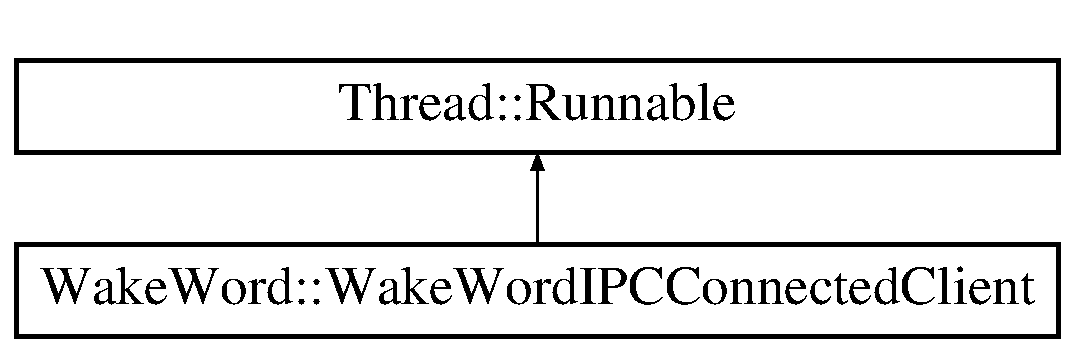
\includegraphics[height=2.000000cm]{d6/d58/classWakeWord_1_1WakeWordIPCConnectedClient}
\end{center}
\end{figure}
\subsection*{Public Member Functions}
\begin{DoxyCompactItemize}
\item 
\mbox{\Hypertarget{classWakeWord_1_1WakeWordIPCConnectedClient_abd6340aa510d15efe94068c304093502}\label{classWakeWord_1_1WakeWordIPCConnectedClient_abd6340aa510d15efe94068c304093502}} 
{\bfseries Wake\+Word\+I\+P\+C\+Connected\+Client} (int client\+\_\+socket, \hyperlink{classWakeWord_1_1WakeWordIPCSocket}{Wake\+Word\+I\+P\+C\+Socket} $\ast$ipc\+\_\+socket)
\item 
\mbox{\Hypertarget{classWakeWord_1_1WakeWordIPCConnectedClient_a253f377db5f5f2ec45ffb73f9ec77a69}\label{classWakeWord_1_1WakeWordIPCConnectedClient_a253f377db5f5f2ec45ffb73f9ec77a69}} 
void {\bfseries init} ()
\item 
\mbox{\Hypertarget{classWakeWord_1_1WakeWordIPCConnectedClient_a0804762a56a4e913d52b90f52fe18c6c}\label{classWakeWord_1_1WakeWordIPCConnectedClient_a0804762a56a4e913d52b90f52fe18c6c}} 
void {\bfseries run} ()
\item 
\mbox{\Hypertarget{classWakeWord_1_1WakeWordIPCConnectedClient_a417514d38af199fc4d3cbc1e4576da5b}\label{classWakeWord_1_1WakeWordIPCConnectedClient_a417514d38af199fc4d3cbc1e4576da5b}} 
void {\bfseries terminate} ()
\item 
\mbox{\Hypertarget{classWakeWord_1_1WakeWordIPCConnectedClient_a4d41fbc28103f82cd9a1ca3569084193}\label{classWakeWord_1_1WakeWordIPCConnectedClient_a4d41fbc28103f82cd9a1ca3569084193}} 
void {\bfseries send\+Command} (I\+P\+C\+Command command)  throw ( std\+::exception )
\end{DoxyCompactItemize}


The documentation for this class was generated from the following files\+:\begin{DoxyCompactItemize}
\item 
/home/mutzi/progs/linux\+\_\+workspace/alexa-\/avs-\/prototype/src/include/wakewordipcconnectedclient.\+h\item 
/home/mutzi/progs/linux\+\_\+workspace/alexa-\/avs-\/prototype/src/wakewordipcconnectedclient.\+cpp\end{DoxyCompactItemize}

\hypertarget{classWakeWord_1_1WakeWordIPCFactory}{}\section{Wake\+Word\+:\+:Wake\+Word\+I\+P\+C\+Factory Class Reference}
\label{classWakeWord_1_1WakeWordIPCFactory}\index{Wake\+Word\+::\+Wake\+Word\+I\+P\+C\+Factory@{Wake\+Word\+::\+Wake\+Word\+I\+P\+C\+Factory}}
\subsection*{Public Member Functions}
\begin{DoxyCompactItemize}
\item 
\mbox{\Hypertarget{classWakeWord_1_1WakeWordIPCFactory_a6e0d90802615e58d1001b3d18cdfcc5a}\label{classWakeWord_1_1WakeWordIPCFactory_a6e0d90802615e58d1001b3d18cdfcc5a}} 
\hyperlink{classWakeWord_1_1WakeWordIPC}{Wake\+Word\+I\+PC} $\ast$ {\bfseries create\+Wake\+Word\+I\+PC} (\hyperlink{classWakeWord_1_1WakeWordDetectedHandler}{Wake\+Word\+Detected\+Handler} $\ast$handler, int port\+Number)  throw ( std\+::exception )
\end{DoxyCompactItemize}


The documentation for this class was generated from the following files\+:\begin{DoxyCompactItemize}
\item 
/home/mutzi/progs/linux\+\_\+workspace/alexa-\/avs-\/prototype/src/include/wakewordipcfactory.\+h\item 
/home/mutzi/progs/linux\+\_\+workspace/alexa-\/avs-\/prototype/src/wakewordipcfactory.\+cpp\end{DoxyCompactItemize}

\hypertarget{classWakeWord_1_1WakeWordIPCSocket}{}\section{Wake\+Word\+:\+:Wake\+Word\+I\+P\+C\+Socket Class Reference}
\label{classWakeWord_1_1WakeWordIPCSocket}\index{Wake\+Word\+::\+Wake\+Word\+I\+P\+C\+Socket@{Wake\+Word\+::\+Wake\+Word\+I\+P\+C\+Socket}}
Inheritance diagram for Wake\+Word\+:\+:Wake\+Word\+I\+P\+C\+Socket\+:\begin{figure}[H]
\begin{center}
\leavevmode
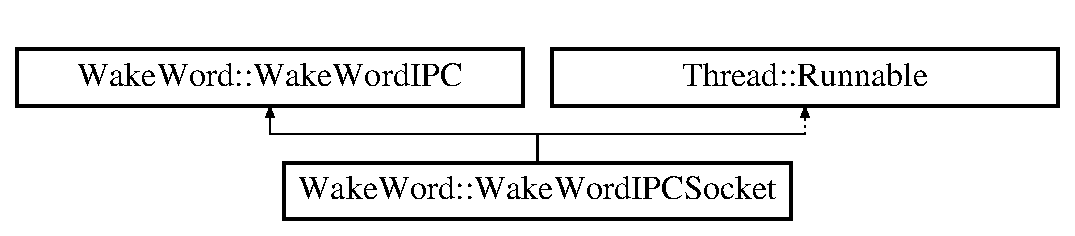
\includegraphics[height=2.000000cm]{d5/d6e/classWakeWord_1_1WakeWordIPCSocket}
\end{center}
\end{figure}
\subsection*{Public Member Functions}
\begin{DoxyCompactItemize}
\item 
\mbox{\Hypertarget{classWakeWord_1_1WakeWordIPCSocket_a92fe280290e8b39513659a7a7e09fe91}\label{classWakeWord_1_1WakeWordIPCSocket_a92fe280290e8b39513659a7a7e09fe91}} 
{\bfseries Wake\+Word\+I\+P\+C\+Socket} (\hyperlink{classWakeWord_1_1WakeWordDetectedHandler}{Wake\+Word\+Detected\+Handler} $\ast$handler, int port\+Number)  throw ( std\+::exception )
\item 
\mbox{\Hypertarget{classWakeWord_1_1WakeWordIPCSocket_afbbb6a3f366cd82d89c2c707033c61ca}\label{classWakeWord_1_1WakeWordIPCSocket_afbbb6a3f366cd82d89c2c707033c61ca}} 
void {\bfseries init} ()
\item 
\mbox{\Hypertarget{classWakeWord_1_1WakeWordIPCSocket_a2dccabdfee1391b187e2e684afd7f50a}\label{classWakeWord_1_1WakeWordIPCSocket_a2dccabdfee1391b187e2e684afd7f50a}} 
void {\bfseries send\+Command} (I\+P\+C\+Command)  throw ( std\+::exception )
\item 
\mbox{\Hypertarget{classWakeWord_1_1WakeWordIPCSocket_a7f5da344af20a9fc26823e9c574a11bf}\label{classWakeWord_1_1WakeWordIPCSocket_a7f5da344af20a9fc26823e9c574a11bf}} 
void {\bfseries run} ()
\item 
\mbox{\Hypertarget{classWakeWord_1_1WakeWordIPCSocket_ab783448eb6eb876fa3d1cc2a1d1ba04a}\label{classWakeWord_1_1WakeWordIPCSocket_ab783448eb6eb876fa3d1cc2a1d1ba04a}} 
void {\bfseries register\+Client} (\hyperlink{classWakeWord_1_1WakeWordIPCConnectedClient}{Wake\+Word\+I\+P\+C\+Connected\+Client} $\ast$new\+\_\+client)
\item 
\mbox{\Hypertarget{classWakeWord_1_1WakeWordIPCSocket_aaf95161a4a1956a886af9cee9f872aee}\label{classWakeWord_1_1WakeWordIPCSocket_aaf95161a4a1956a886af9cee9f872aee}} 
void {\bfseries unregister\+Client} (\hyperlink{classWakeWord_1_1WakeWordIPCConnectedClient}{Wake\+Word\+I\+P\+C\+Connected\+Client} $\ast$old\+\_\+client)
\item 
\mbox{\Hypertarget{classWakeWord_1_1WakeWordIPCSocket_aa536d8b204fdfa6f2ffd38e8c23c2e77}\label{classWakeWord_1_1WakeWordIPCSocket_aa536d8b204fdfa6f2ffd38e8c23c2e77}} 
void {\bfseries process\+Wake\+Word\+Detected} ()
\end{DoxyCompactItemize}
\subsection*{Static Public Attributes}
\begin{DoxyCompactItemize}
\item 
\mbox{\Hypertarget{classWakeWord_1_1WakeWordIPCSocket_a3fb9ddc9d8457219f09b923a9ed21f7b}\label{classWakeWord_1_1WakeWordIPCSocket_a3fb9ddc9d8457219f09b923a9ed21f7b}} 
static \hyperlink{classLogger}{Logger} \& {\bfseries log} = Logger\+::instance()
\end{DoxyCompactItemize}
\subsection*{Additional Inherited Members}


The documentation for this class was generated from the following files\+:\begin{DoxyCompactItemize}
\item 
/home/mutzi/progs/linux\+\_\+workspace/alexa-\/avs-\/prototype/src/include/wakewordipcsocket.\+h\item 
/home/mutzi/progs/linux\+\_\+workspace/alexa-\/avs-\/prototype/src/wakewordipcsocket.\+cpp\end{DoxyCompactItemize}

\hypertarget{classWakeWord_1_1WakeWordReadyInterface}{}\section{Wake\+Word\+:\+:Wake\+Word\+Ready\+Interface Class Reference}
\label{classWakeWord_1_1WakeWordReadyInterface}\index{Wake\+Word\+::\+Wake\+Word\+Ready\+Interface@{Wake\+Word\+::\+Wake\+Word\+Ready\+Interface}}
\subsection*{Public Member Functions}
\begin{DoxyCompactItemize}
\item 
\mbox{\Hypertarget{classWakeWord_1_1WakeWordReadyInterface_a19e66fc2d8fc807d1d8bdf636a0565ef}\label{classWakeWord_1_1WakeWordReadyInterface_a19e66fc2d8fc807d1d8bdf636a0565ef}} 
virtual void {\bfseries on\+Wake\+Word\+Ready} ()=0
\item 
\mbox{\Hypertarget{classWakeWord_1_1WakeWordReadyInterface_ae98bf3af62b41e28f491f623f0748488}\label{classWakeWord_1_1WakeWordReadyInterface_ae98bf3af62b41e28f491f623f0748488}} 
virtual void {\bfseries on\+Wake\+Word\+Not\+Ready} ()=0
\end{DoxyCompactItemize}


The documentation for this class was generated from the following file\+:\begin{DoxyCompactItemize}
\item 
/home/mutzi/progs/linux\+\_\+workspace/alexa-\/avs-\/prototype/src/include/wakewordreadyinterface.\+h\end{DoxyCompactItemize}

%--- End generated contents ---

% Index
\backmatter
\newpage
\phantomsection
\clearemptydoublepage
\addcontentsline{toc}{chapter}{Index}
\printindex

\end{document}
